% Options for packages loaded elsewhere
\PassOptionsToPackage{unicode}{hyperref}
\PassOptionsToPackage{hyphens}{url}
\PassOptionsToPackage{dvipsnames,svgnames,x11names}{xcolor}
%
\documentclass[
  letterpaper,
  krantz2]{krantz}

\usepackage{amsmath,amssymb}
\usepackage{iftex}
\ifPDFTeX
  \usepackage[T1]{fontenc}
  \usepackage[utf8]{inputenc}
  \usepackage{textcomp} % provide euro and other symbols
\else % if luatex or xetex
  \usepackage{unicode-math}
  \defaultfontfeatures{Scale=MatchLowercase}
  \defaultfontfeatures[\rmfamily]{Ligatures=TeX,Scale=1}
\fi
\usepackage{lmodern}
\ifPDFTeX\else  
    % xetex/luatex font selection
\fi
% Use upquote if available, for straight quotes in verbatim environments
\IfFileExists{upquote.sty}{\usepackage{upquote}}{}
\IfFileExists{microtype.sty}{% use microtype if available
  \usepackage[]{microtype}
  \UseMicrotypeSet[protrusion]{basicmath} % disable protrusion for tt fonts
}{}
\makeatletter
\@ifundefined{KOMAClassName}{% if non-KOMA class
  \IfFileExists{parskip.sty}{%
    \usepackage{parskip}
  }{% else
    \setlength{\parindent}{0pt}
    \setlength{\parskip}{6pt plus 2pt minus 1pt}}
}{% if KOMA class
  \KOMAoptions{parskip=half}}
\makeatother
\usepackage{xcolor}
\setlength{\emergencystretch}{3em} % prevent overfull lines
\setcounter{secnumdepth}{5}
% Make \paragraph and \subparagraph free-standing
\ifx\paragraph\undefined\else
  \let\oldparagraph\paragraph
  \renewcommand{\paragraph}[1]{\oldparagraph{#1}\mbox{}}
\fi
\ifx\subparagraph\undefined\else
  \let\oldsubparagraph\subparagraph
  \renewcommand{\subparagraph}[1]{\oldsubparagraph{#1}\mbox{}}
\fi

%\usepackage{color}
\usepackage{fancyvrb}
\newcommand{\VerbBar}{|}
\newcommand{\VERB}{\Verb[commandchars=\\\{\}]}
\DefineVerbatimEnvironment{Highlighting}{Verbatim}{commandchars=\\\{\}}
% Add ',fontsize=\small' for more characters per line
\usepackage{framed}
\definecolor{shadecolor}{RGB}{241,243,245}
\newenvironment{Shaded}{\begin{snugshade}}{\end{snugshade}}
\newcommand{\AlertTok}[1]{\textcolor[rgb]{0.68,0.00,0.00}{#1}}
\newcommand{\AnnotationTok}[1]{\textcolor[rgb]{0.37,0.37,0.37}{#1}}
\newcommand{\AttributeTok}[1]{\textcolor[rgb]{0.40,0.45,0.13}{#1}}
\newcommand{\BaseNTok}[1]{\textcolor[rgb]{0.68,0.00,0.00}{#1}}
\newcommand{\BuiltInTok}[1]{\textcolor[rgb]{0.00,0.23,0.31}{#1}}
\newcommand{\CharTok}[1]{\textcolor[rgb]{0.13,0.47,0.30}{#1}}
\newcommand{\CommentTok}[1]{\textcolor[rgb]{0.37,0.37,0.37}{#1}}
\newcommand{\CommentVarTok}[1]{\textcolor[rgb]{0.37,0.37,0.37}{\textit{#1}}}
\newcommand{\ConstantTok}[1]{\textcolor[rgb]{0.56,0.35,0.01}{#1}}
\newcommand{\ControlFlowTok}[1]{\textcolor[rgb]{0.00,0.23,0.31}{#1}}
\newcommand{\DataTypeTok}[1]{\textcolor[rgb]{0.68,0.00,0.00}{#1}}
\newcommand{\DecValTok}[1]{\textcolor[rgb]{0.68,0.00,0.00}{#1}}
\newcommand{\DocumentationTok}[1]{\textcolor[rgb]{0.37,0.37,0.37}{\textit{#1}}}
\newcommand{\ErrorTok}[1]{\textcolor[rgb]{0.68,0.00,0.00}{#1}}
\newcommand{\ExtensionTok}[1]{\textcolor[rgb]{0.00,0.23,0.31}{#1}}
\newcommand{\FloatTok}[1]{\textcolor[rgb]{0.68,0.00,0.00}{#1}}
\newcommand{\FunctionTok}[1]{\textcolor[rgb]{0.28,0.35,0.67}{#1}}
\newcommand{\ImportTok}[1]{\textcolor[rgb]{0.00,0.46,0.62}{#1}}
\newcommand{\InformationTok}[1]{\textcolor[rgb]{0.37,0.37,0.37}{#1}}
\newcommand{\KeywordTok}[1]{\textcolor[rgb]{0.00,0.23,0.31}{#1}}
\newcommand{\NormalTok}[1]{\textcolor[rgb]{0.00,0.23,0.31}{#1}}
\newcommand{\OperatorTok}[1]{\textcolor[rgb]{0.37,0.37,0.37}{#1}}
\newcommand{\OtherTok}[1]{\textcolor[rgb]{0.00,0.23,0.31}{#1}}
\newcommand{\PreprocessorTok}[1]{\textcolor[rgb]{0.68,0.00,0.00}{#1}}
\newcommand{\RegionMarkerTok}[1]{\textcolor[rgb]{0.00,0.23,0.31}{#1}}
\newcommand{\SpecialCharTok}[1]{\textcolor[rgb]{0.37,0.37,0.37}{#1}}
\newcommand{\SpecialStringTok}[1]{\textcolor[rgb]{0.13,0.47,0.30}{#1}}
\newcommand{\StringTok}[1]{\textcolor[rgb]{0.13,0.47,0.30}{#1}}
\newcommand{\VariableTok}[1]{\textcolor[rgb]{0.07,0.07,0.07}{#1}}
\newcommand{\VerbatimStringTok}[1]{\textcolor[rgb]{0.13,0.47,0.30}{#1}}
\newcommand{\WarningTok}[1]{\textcolor[rgb]{0.37,0.37,0.37}{\textit{#1}}}

\providecommand{\tightlist}{%
  \setlength{\itemsep}{0pt}\setlength{\parskip}{0pt}}\usepackage{longtable,booktabs,array}
\usepackage{calc} % for calculating minipage widths
% Correct order of tables after \paragraph or \subparagraph
\usepackage{etoolbox}
\makeatletter
\patchcmd\longtable{\par}{\if@noskipsec\mbox{}\fi\par}{}{}
\makeatother
% Allow footnotes in longtable head/foot
\IfFileExists{footnotehyper.sty}{\usepackage{footnotehyper}}{\usepackage{footnote}}
\makesavenoteenv{longtable}
\usepackage{graphicx}
\makeatletter
\def\maxwidth{\ifdim\Gin@nat@width>\linewidth\linewidth\else\Gin@nat@width\fi}
\def\maxheight{\ifdim\Gin@nat@height>\textheight\textheight\else\Gin@nat@height\fi}
\makeatother
% Scale images if necessary, so that they will not overflow the page
% margins by default, and it is still possible to overwrite the defaults
% using explicit options in \includegraphics[width, height, ...]{}
\setkeys{Gin}{width=\maxwidth,height=\maxheight,keepaspectratio}
% Set default figure placement to htbp
\makeatletter
\def\fps@figure{htbp}
\makeatother
\newlength{\cslhangindent}
\setlength{\cslhangindent}{1.5em}
\newlength{\csllabelwidth}
\setlength{\csllabelwidth}{3em}
\newlength{\cslentryspacingunit} % times entry-spacing
\setlength{\cslentryspacingunit}{\parskip}
\newenvironment{CSLReferences}[2] % #1 hanging-ident, #2 entry spacing
 {% don't indent paragraphs
  \setlength{\parindent}{0pt}
  % turn on hanging indent if param 1 is 1
  \ifodd #1
  \let\oldpar\par
  \def\par{\hangindent=\cslhangindent\oldpar}
  \fi
  % set entry spacing
  \setlength{\parskip}{#2\cslentryspacingunit}
 }%
 {}
\usepackage{calc}
\newcommand{\CSLBlock}[1]{#1\hfill\break}
\newcommand{\CSLLeftMargin}[1]{\parbox[t]{\csllabelwidth}{#1}}
\newcommand{\CSLRightInline}[1]{\parbox[t]{\linewidth - \csllabelwidth}{#1}\break}
\newcommand{\CSLIndent}[1]{\hspace{\cslhangindent}#1}

\usepackage{makeidx}
\makeindex
\makeatletter
\@ifpackageloaded{tcolorbox}{}{\usepackage[skins,breakable]{tcolorbox}}
\@ifpackageloaded{fontawesome5}{}{\usepackage{fontawesome5}}
\definecolor{quarto-callout-color}{HTML}{909090}
\definecolor{quarto-callout-note-color}{HTML}{0758E5}
\definecolor{quarto-callout-important-color}{HTML}{CC1914}
\definecolor{quarto-callout-warning-color}{HTML}{EB9113}
\definecolor{quarto-callout-tip-color}{HTML}{00A047}
\definecolor{quarto-callout-caution-color}{HTML}{FC5300}
\definecolor{quarto-callout-color-frame}{HTML}{acacac}
\definecolor{quarto-callout-note-color-frame}{HTML}{4582ec}
\definecolor{quarto-callout-important-color-frame}{HTML}{d9534f}
\definecolor{quarto-callout-warning-color-frame}{HTML}{f0ad4e}
\definecolor{quarto-callout-tip-color-frame}{HTML}{02b875}
\definecolor{quarto-callout-caution-color-frame}{HTML}{fd7e14}
\makeatother
\makeatletter
\makeatother
\makeatletter
\@ifpackageloaded{bookmark}{}{\usepackage{bookmark}}
\makeatother
\makeatletter
\@ifpackageloaded{caption}{}{\usepackage{caption}}
\AtBeginDocument{%
\ifdefined\contentsname
  \renewcommand*\contentsname{Table of contents}
\else
  \newcommand\contentsname{Table of contents}
\fi
\ifdefined\listfigurename
  \renewcommand*\listfigurename{List of Figures}
\else
  \newcommand\listfigurename{List of Figures}
\fi
\ifdefined\listtablename
  \renewcommand*\listtablename{List of Tables}
\else
  \newcommand\listtablename{List of Tables}
\fi
\ifdefined\figurename
  \renewcommand*\figurename{Figure}
\else
  \newcommand\figurename{Figure}
\fi
\ifdefined\tablename
  \renewcommand*\tablename{Table}
\else
  \newcommand\tablename{Table}
\fi
}
\@ifpackageloaded{float}{}{\usepackage{float}}
\floatstyle{ruled}
\@ifundefined{c@chapter}{\newfloat{codelisting}{h}{lop}}{\newfloat{codelisting}{h}{lop}[chapter]}
\floatname{codelisting}{Listing}
\newcommand*\listoflistings{\listof{codelisting}{List of Listings}}
\makeatother
\makeatletter
\@ifpackageloaded{caption}{}{\usepackage{caption}}
\@ifpackageloaded{subcaption}{}{\usepackage{subcaption}}
\makeatother
\makeatletter
\@ifpackageloaded{tcolorbox}{}{\usepackage[skins,breakable]{tcolorbox}}
\makeatother
\makeatletter
\@ifundefined{shadecolor}{\definecolor{shadecolor}{HTML}{f2f2f2}}
\makeatother
\makeatletter
\@ifundefined{codebgcolor}{\definecolor{codebgcolor}{HTML}{f2f2f2}}
\makeatother
\makeatletter
\@ifpackageloaded{sidenotes}{}{\usepackage{sidenotes}}
\@ifpackageloaded{marginnote}{}{\usepackage{marginnote}}
\makeatother
\makeatletter
\makeatother
\ifLuaTeX
  \usepackage{selnolig}  % disable illegal ligatures
\fi
\IfFileExists{bookmark.sty}{\usepackage{bookmark}}{\usepackage{hyperref}}
\IfFileExists{xurl.sty}{\usepackage{xurl}}{} % add URL line breaks if available
\urlstyle{same} % disable monospaced font for URLs
\hypersetup{
  pdftitle={Applied Machine Learning Using mlr3 in R},
  colorlinks=true,
  linkcolor={black},
  filecolor={Maroon},
  citecolor={Blue},
  urlcolor={blue},
  pdfcreator={LaTeX via pandoc}}

\title{Applied Machine Learning Using mlr3 in R}
\author{}
\date{}

\begin{document}
\maketitle
\ifdefined\Shaded\renewenvironment{Shaded}{\begin{tcolorbox}[boxrule=0pt, sharp corners, breakable, borderline west={3pt}{0pt}{shadecolor}, frame hidden, enhanced, colback={codebgcolor}]}{\end{tcolorbox}}\fi

\bookmarksetup{startatroot}

\frontmatter

\halftitle{Main Title}{Standard blurb goes here}\%\%Placeholder for Half
title

\seriespg{Series page goes here (if applicable); otherwise blank}

\title{Applied Machine Learning Using mlr3 in R}

\edition{First Edition}

\editor{Bernd Bischl, Raphael Sonabend, Lars Kotthoff, Michel Lang}

\locpage

\cleardoublepage
\setcounter{page}{7}

\tableofcontents

\chapter*{Preface}

The \href{https://cran.r-project.org/package=mlr}{\texttt{mlr}}\index{\texttt{mlr}}
package (Bischl et al. 2016) was first released on CRAN in 2013, with
the core design and architecture dating back further. Over time, the
addition of many features led to a complex design that made it too
difficult for us to extend further. In hindsight, we saw that some
design and architecture choices in
\href{https://cran.r-project.org/package=mlr}{\texttt{mlr}} made it
difficult to support new features, in particular with respect to ML
pipelines. So in 2018, we set about working on a reimplementation, which
resulted in the first release of
\href{https://mlr3.mlr-org.com}{\texttt{mlr3}}\index{\texttt{mlr3}} on
CRAN in July 2019.

\subsection*{Overview}

The \texttt{mlr3} ecosystem is the result of many years of
methodological and applied research. This book describes the resulting
features and discusses best practices for ML, technical implementation
details, and in-depth considerations for model optimization. This book
may be helpful for both practitioners who want to quickly apply machine
learning (ML) algorithms and researchers who want to implement,
benchmark, and compare their new methods in a structured environment.
While we hope this book is accessible to a wide range of readers and
levels of ML expertise, we do assume that readers have taken at least an
introductory ML course or have the equivalent expertise and some basic
experience with R. A background in computer science or statistics is
beneficial for understanding the advanced functionality described in the
later chapters of this book, but not required. A comprehensive ML
introduction for those new to the field can be found in James et al.
(2014). Wickham and Grolemund (2017) provides a comprehensive
introduction to data science in R.

The book is split into the following four parts:

\textbf{Part I: Fundamentals} In this part of the book we will teach you
the fundamentals of \texttt{mlr3}. This will give you a flavor of the
building blocks of the \texttt{mlr3} universe and the basic tools you
will need to tackle most machine learning problems. We recommend that
all readers study these chapters to become familiar with \texttt{mlr3}
terminology, syntax, and style. In Chapter~\ref{sec-basics} we will
cover the basic classes in
\href{https://mlr3.mlr-org.com}{\texttt{mlr3}}\index{\texttt{mlr3}},
including \texttt{Learner} (machine learning implementations),
\texttt{Measure} (performance metrics), and \texttt{Task} (machine
learning task definitions). Chapter~\ref{sec-performance} will take
evaluation a step further to include discussions about resampling --
robust strategies for measuring model performance -- and benchmarking --
experiments for comparing multiple models.

\textbf{Part II: Tuning and Feature Selection} In this part of the book,
we will look at more advanced methodology that is essential to
developing powerful ML models with good predictive ability.
Chapter~\ref{sec-optimization} introduces hyperparameter optimization,
which is the process of tuning model hyperparameters to obtain better
model performance. Tuning is implemented via the
\href{https://mlr3tuning.mlr-org.com}{\texttt{mlr3tuning}}\index{\texttt{mlr3tuning}}
package, which also includes methods for automating complex tuning
processes, including nested resampling. The performance of ML models can
be improved by tuning hyperparameters but also by carefully selecting
features. Chapter~\ref{sec-feature-selection} introduces feature
selection with filters and wrappers implemented in
\href{https://mlr3filters.mlr-org.com}{\texttt{mlr3filters}}\index{\texttt{mlr3filters}}
and
\href{https://mlr3fselect.mlr-org.com}{\texttt{mlr3fselect}}\index{\texttt{mlr3fselect}}.
For readers interested in taking a deep dive into tuning,
Chapter~\ref{sec-optimization-advanced} discusses advanced tuning
methods including error handling, multi-objective tuning, and tuning
with Hyperband and Bayesian optimization methods.

\textbf{Part III: Pipelines and Preprocessing} In Part III we introduce
\href{https://mlr3pipelines.mlr-org.com}{\texttt{mlr3pipelines}}\index{\texttt{mlr3pipelines}},
which allows users to implement complex ML workflows easily. In
Chapter~\ref{sec-pipelines} we will show you how to build a pipeline out
of discrete configurable operations and how to treat complex pipelines
as if they were any other machine learning model. In
Chapter~\ref{sec-pipelines-nonseq} we will build on the previous chapter
by introducing non-sequential pipelines, which can have multiple
branches that carry out operations concurrently. We will also
demonstrate how to tune pipelines, including how to tune which
operations should be included in the pipeline. Finally, in
Chapter~\ref{sec-preprocessing} we will put pipelines into practice by
demonstrating how to solve common problems that occur when fitting ML
models to messy data.

\textbf{Part IV: Advanced Topics} In the final part of the book, we will
look at advanced methodology and technical details. This part of the
book is more theory-heavy in some sections to help ground the design and
implementation decisions. We will begin by looking at advanced technical
details in Chapter~\ref{sec-technical} that are essential reading for
advanced users who require parallelization, custom error handling, or
large databases. Chapter~\ref{sec-large-benchmarking} will build on all
preceding chapters to introduce large-scale benchmarking experiments
that compare many models, tasks, and measures; including how to make use
of \texttt{mlr3} extension packages for loading data, using
high-performance computing clusters, and formal statistical analysis of
benchmark experiments. Chapter~\ref{sec-interpretation} will discuss
different packages that are compatible with \texttt{mlr3} to provide
model-agnostic interpretability for feature importance and local
explainability of individual predictions. Chapter~\ref{sec-special} will
then delve into detail on domain-specific methods that are implemented
in our extension packages including survival analysis, density
estimation, spatio-temporal analysis, and more. Readers may choose to
selectively read sections in this chapter depending on your use case
(i.e., if you have domain-specific problems to tackle), or to use these
as introductions to new domains to explore. Finally,
Chapter~\ref{sec-fairness} will introduce algorithmic fairness, which
includes specialized measures and methods to identify and reduce
algorithmic biases.

\subsection*{Citing this book}

This book is the culmination of many years worth of software design,
coding, writing, and editing. It is very important to us that all our
contributors are credited appropriately.

Citation details of packages in the \texttt{mlr3} ecosystem can be found
in their respective GitHub repositories.

When you are citing this book please cite chapters directly; citations
can be found at the end of each chapter. If you need to reference the
full book please use:

\begin{verbatim}
Bischl, B., Sonabend, R., Kotthoff, L., & Lang, M. (Eds.). (2024).
"Applied Machine Learning Using mlr3 in R". CRC Press. https://mlr3book.mlr-org.com

@book{Bischl2024
    title = Applied Machine Learning Using mlr3 in R
    editor = {Bernd Bischl, Raphael Sonabend, Lars Kotthoff, Michel Lang},
    url = {https://mlr3book.mlr-org.com},
    year = {2024},
    isbn = {9781032507545},
    publisher = {CRC Press}
}
\end{verbatim}

Please see the front page of the book website
(\url{https://mlr3book.mlr-org.com}) for full licensing details.

\vspace{10mm}

We hope you enjoy reading this book.

\vspace{5mm}

Bernd, Raphael, Lars, Michel

\chapter*{Editors}

Bernd Bischl is a professor of Statistical Learning and Data Science in
LMU Munich and co-director of the Munich Center for Machine Learning. He
studied Computer Science, Artificial Intelligence and Data Science and
holds a PhD in Statistics. His research interests include AutoML, model
selection, interpretable ML and the development of statistical software.
He wrote the initial version of \texttt{mlr} in 2012 and 2013 and still
leads the team of developers of \texttt{mlr3}, now largely focusing on
design, code review and strategic development.

Raphael Sonabend is a Visiting Researcher at Imperial College London and
an Open Source Manager at Genomics England. They hold a PhD in
statistics, specializing in machine learning applications for survival
analysis. They wrote the \texttt{mlr3} packages \texttt{mlr3proba} and
\texttt{mlr3benchmark}.

Lars Kotthoff is an associate professor of Computer Science at the
University of Wyoming, US. He has studied and held academic appointments
in Germany, UK, Ireland, and Canada. Lars has been contributing to
\texttt{mlr} for about a decade. His research aims to automate machine
learning and other areas of AI.

Michel Lang is the scientific coordinator of the Research Center
Trustworthy Data Science and Security. He has a PhD in Statistics and
has been developing statistical software for over a decade. He joined
the \texttt{mlr} team in 2014 and wrote the initial version of
\texttt{mlr3}.

\begin{contributorlist}

\contau{Marc Becker}
\contaff{Ludwig-Maximilians-Universität München}

\contau{Przemysław Biecek}
\contaff{MI2.AI, Warsaw University of Technology}
\contaff{University of Warsaw}

\contau{Martin Binder}
\contaff{Ludwig-Maximilians-Universität München}
\contaff{Munich Center for Machine Learning (MCML)}

\contau{Bernd Bischl}
\contaff{Ludwig-Maximilians-Universität München}
\contaff{Munich Center for Machine Learning (MCML)}

\contau{Lukas Burk}
\contaff{Ludwig-Maximilians-Universität München}
\contaff{Leibniz Institute for Prevention Research and Epidemiology - BIPS}
\contaff{Munich Center for Machine Learning (MCML)}

\contau{Giuseppe Casalicchio}
\contaff{Ludwig-Maximilians-Universität München}
\contaff{Munich Center for Machine Learning (MCML)}
\contaff{Essential Data Science Training GmbH}

\contau{Susanne Dandl}
\contaff{Ludwig-Maximilians-Universität München}
\contaff{Munich Center for Machine Learning (MCML)}

\contau{Sebastian Fischer}
\contaff{Ludwig-Maximilians-Universität München}

\contau{Natalie Foss}
\contaff{University of Wyoming}

\contau{Lars Kotthoff}
\contaff{University of Wyoming}

\contau{Michel Lang}
\contaff{Research Center Trustworthy Data Science and Security}
\contaff{TU Dortmund University}

\contau{Florian Pfisterer}
\contaff{Ludwig-Maximilians-Universität München}

\contau{Damir Pulatov}
\contaff{University of Wyoming}

\contau{Lennart Schneider}
\contaff{Ludwig-Maximilians-Universität München}
\contaff{Munich Center for Machine Learning (MCML)}

\contau{Patrick Schratz}
\contaff{Friedrich Schiller University Jena}

\contau{Raphael Sonabend}
\contaff{Imperial College London}

\contau{Janek Thomas}
\contaff{Ludwig-Maximilians-Universität München}
\contaff{Munich Center for Machine Learning (MCML)}
\contaff{Essential Data Science Training GmbH}

\contau{Marvin N. Wright}
\contaff{Leibniz Institute for Prevention Research and Epidemiology – BIPS}
\contaff{University of Bremen}
\contaff{University of Copenhagen}

\end{contributorlist}

\mainmatter

\bookmarksetup{startatroot}

\hypertarget{sec-introduction}{%
\chapter{Introduction and Overview}\label{sec-introduction}}

\vspace{-15mm}\addtocontents{toc}{\textit{Lars Kotthoff, Raphael Sonabend, Natalie Foss and Bernd Bischl}}

\textbf{Lars Kotthoff} \newline  \emph{University of Wyoming}

\textbf{Raphael Sonabend} \newline  \emph{Imperial College London}

\textbf{Natalie Foss} \newline  \emph{University of Wyoming}

\textbf{Bernd Bischl} \newline  \emph{Ludwig-Maximilians-Universität
München, and Munich Center for Machine Learning (MCML)}
\newline \newline 

Welcome to the \textbf{M}achine \textbf{L}earning in \textbf{R}
universe. In this book, we will guide you through the functionality
offered by \texttt{mlr3} step by step. If you want to contribute to our
universe, ask any questions, read documentation, or just chat with the
team, head to \url{https://github.com/mlr-org/mlr3} which has several
useful links in the README.

The \href{https://mlr3.mlr-org.com}{\texttt{mlr3}}\index{\texttt{mlr3}}
(Lang et al. 2019) package and the wider \texttt{mlr3} ecosystem provide
a generic, object-oriented\index{object-oriented programming}, and
extensible framework for regression\index{regression}
(Section~\ref{sec-tasks}), classification\index{classification}
(Section~\ref{sec-classif}), and other machine learning
tasks\index{tasks} (Chapter~\ref{sec-special}) for the R language (R
Core Team 2019). On the most basic level, the unified interface provides
functionality to train, test, and evaluate many machine learning
algorithms. You can also take this a step further with hyperparameter
optimization, computational pipelines, model interpretation, and much
more. \texttt{mlr3} has similar overall aims to \texttt{caret} and
\texttt{tidymodels} for R, \texttt{scikit-learn} for Python, and
\texttt{MLJ} for Julia. In general,
\href{https://mlr3.mlr-org.com}{\texttt{mlr3}}\index{\texttt{mlr3}} is
designed to provide more flexibility than other ML frameworks while
still offering easy ways to use advanced functionality. While
\texttt{tidymodels} in particular makes it very easy to perform simple
ML tasks,
\href{https://mlr3.mlr-org.com}{\texttt{mlr3}}\index{\texttt{mlr3}} is
more geared towards advanced ML.

Before we can show you the full power of \texttt{mlr3}, we recommend
installing the
\href{https://mlr3verse.mlr-org.com}{\texttt{mlr3verse}}\index{\texttt{mlr3verse}}
package, which will install several, important packages in the
\texttt{mlr3} ecosystem.

\begin{Shaded}
\begin{Highlighting}[]
\FunctionTok{install.packages}\NormalTok{(}\StringTok{"mlr3verse"}\NormalTok{)}
\end{Highlighting}
\end{Shaded}

\hypertarget{installguide}{%
\section{Installation Guidelines}\label{installguide}}

There are many packages in the \texttt{mlr3} ecosystem that you may want
to use as you work through this book. All our packages can be installed
from GitHub and R-universe\footnote{R-universe is an alternative package
  repository to CRAN. The bit of code below tells R to look at both
  R-universe and CRAN when trying to install packages. R will always
  install the latest version of a package.}; the majority (but not all)
packages can also be installed from CRAN. We recommend adding the
mlr-org R-universe to your R options so you can install all packages
with \texttt{install.packages()}, without having to worry which package
repository it comes from. To do this, install
\href{https://cran.r-project.org/package=usethis}{\texttt{usethis}} and
run the following:

\begin{Shaded}
\begin{Highlighting}[]
\NormalTok{usethis}\SpecialCharTok{::}\FunctionTok{edit\_r\_profile}\NormalTok{()}
\end{Highlighting}
\end{Shaded}

In the file that opens add or change the \texttt{repos} argument in
\texttt{options} so it looks something like the code below (you might
need to add the full code block below or just edit the existing
\texttt{options} function).

\begin{Shaded}
\begin{Highlighting}[]
\FunctionTok{options}\NormalTok{(}\AttributeTok{repos =} \FunctionTok{c}\NormalTok{(}
  \AttributeTok{mlrorg =} \StringTok{"https://mlr{-}org.r{-}universe.dev"}\NormalTok{,}
  \AttributeTok{CRAN =} \StringTok{"https://cloud.r{-}project.org/"}
\NormalTok{))}
\end{Highlighting}
\end{Shaded}

Save the file, restart your R session, and you are ready to go!

If you want the latest development version of any of our packages, run

\begin{Shaded}
\begin{Highlighting}[]
\NormalTok{remotes}\SpecialCharTok{::}\FunctionTok{install\_github}\NormalTok{(}\StringTok{"mlr{-}org/\{pkg\}"}\NormalTok{)}
\end{Highlighting}
\end{Shaded}

with \texttt{\{pkg\}} replaced with the name of the package you want to
install. You can see an up-to-date list of all our extension packages at
\url{https://github.com/mlr-org/mlr3/wiki/Extension-Packages}.

\hypertarget{howtouse}{%
\section{How to Use This Book}\label{howtouse}}

The \texttt{mlr3} ecosystem is the result of many years of
methodological and applied research. This book describes the resulting
features and discusses best practices for ML, technical implementation
details, and in-depth considerations for model optimization. This book
may be helpful for both practitioners who want to quickly apply machine
learning (ML) algorithms and researchers who want to implement,
benchmark, and compare their new methods in a structured environment.
While we hope this book is accessible to a wide range of readers and
levels of ML expertise, we do assume that readers have taken at least an
introductory ML course or have the equivalent expertise and some basic
experience with R. A background in computer science or statistics is
beneficial for understanding the advanced functionality described in the
later chapters of this book, but not required. A comprehensive ML
introduction for those new to the field can be found in James et al.
(2014). Wickham and Grolemund (2017) provides a comprehensive
introduction to data science in R.

The book is split into the following four parts:

\textbf{Part I: Fundamentals} In this part of the book we will teach you
the fundamentals of \texttt{mlr3}. This will give you a flavor of the
building blocks of the \texttt{mlr3} universe and the basic tools you
will need to tackle most machine learning problems. We recommend that
all readers study these chapters to become familiar with \texttt{mlr3}
terminology, syntax, and style. In Chapter~\ref{sec-basics} we will
cover the basic classes in
\href{https://mlr3.mlr-org.com}{\texttt{mlr3}}\index{\texttt{mlr3}},
including \texttt{Learner} (machine learning implementations),
\texttt{Measure} (performance metrics), and \texttt{Task} (machine
learning task definitions). Chapter~\ref{sec-performance} will take
evaluation a step further to include discussions about resampling --
robust strategies for measuring model performance -- and benchmarking --
experiments for comparing multiple models.

\textbf{Part II: Tuning and Feature Selection} In this part of the book,
we will look at more advanced methodology that is essential to
developing powerful ML models with good predictive ability.
Chapter~\ref{sec-optimization} introduces hyperparameter optimization,
which is the process of tuning model hyperparameters to obtain better
model performance. Tuning is implemented via the
\href{https://mlr3tuning.mlr-org.com}{\texttt{mlr3tuning}}\index{\texttt{mlr3tuning}}
package, which also includes methods for automating complex tuning
processes, including nested resampling. The performance of ML models can
be improved by tuning hyperparameters but also by carefully selecting
features. Chapter~\ref{sec-feature-selection} introduces feature
selection with filters and wrappers implemented in
\href{https://mlr3filters.mlr-org.com}{\texttt{mlr3filters}}\index{\texttt{mlr3filters}}
and
\href{https://mlr3fselect.mlr-org.com}{\texttt{mlr3fselect}}\index{\texttt{mlr3fselect}}.
For readers interested in taking a deep dive into tuning,
Chapter~\ref{sec-optimization-advanced} discusses advanced tuning
methods including error handling, multi-objective tuning, and tuning
with Hyperband and Bayesian optimization methods.

\textbf{Part III: Pipelines and Preprocessing} In Part III we introduce
\href{https://mlr3pipelines.mlr-org.com}{\texttt{mlr3pipelines}}\index{\texttt{mlr3pipelines}},
which allows users to implement complex ML workflows easily. In
Chapter~\ref{sec-pipelines} we will show you how to build a pipeline out
of discrete configurable operations and how to treat complex pipelines
as if they were any other machine learning model. In
Chapter~\ref{sec-pipelines-nonseq} we will build on the previous chapter
by introducing non-sequential pipelines, which can have multiple
branches that carry out operations concurrently. We will also
demonstrate how to tune pipelines, including how to tune which
operations should be included in the pipeline. Finally, in
Chapter~\ref{sec-preprocessing} we will put pipelines into practice by
demonstrating how to solve common problems that occur when fitting ML
models to messy data.

\textbf{Part IV: Advanced Topics} In the final part of the book, we will
look at advanced methodology and technical details. This part of the
book is more theory-heavy in some sections to help ground the design and
implementation decisions. We will begin by looking at advanced technical
details in Chapter~\ref{sec-technical} that are essential reading for
advanced users who require parallelization, custom error handling, or
large databases. Chapter~\ref{sec-large-benchmarking} will build on all
preceding chapters to introduce large-scale benchmarking experiments
that compare many models, tasks, and measures; including how to make use
of \texttt{mlr3} extension packages for loading data, using
high-performance computing clusters, and formal statistical analysis of
benchmark experiments. Chapter~\ref{sec-interpretation} will discuss
different packages that are compatible with \texttt{mlr3} to provide
model-agnostic interpretability for feature importance and local
explainability of individual predictions. Chapter~\ref{sec-special} will
then delve into detail on domain-specific methods that are implemented
in our extension packages including survival analysis, density
estimation, spatio-temporal analysis, and more. Readers may choose to
selectively read sections in this chapter depending on your use case
(i.e., if you have domain-specific problems to tackle), or to use these
as introductions to new domains to explore. Finally,
Chapter~\ref{sec-fairness} will introduce algorithmic fairness, which
includes specialized measures and methods to identify and reduce
algorithmic biases.

We have marked sections that are particularly complex with respect to
either technical or methodological detail and could be skipped on a
first read with the following information box:

\begin{tcolorbox}[enhanced jigsaw, colframe=quarto-callout-note-color-frame, rightrule=.15mm, bottomrule=.15mm, toprule=.15mm, opacityback=0, colback=white, left=2mm, arc=.35mm, breakable, leftrule=.75mm]
\begin{minipage}[t]{5.5mm}
\textcolor{quarto-callout-note-color}{\faInfo}
\end{minipage}%
\begin{minipage}[t]{\textwidth - 5.5mm}

\textbf{This section covers advanced ML or technical
details.}\vspace{2mm}

\end{minipage}%
\end{tcolorbox}

Each chapter includes examples, API references, and explanations of
methodologies. At the end of each part of the book we have included
exercises for you to test yourself on what you have learned; you can
find the solutions to these exercises at
\url{https://mlr3book.mlr-org.com/solutions.html}. We have marked more
challenging (and possibly time-consuming) exercises with an asterisk,
'*'.

If you want more detail about any of the tasks used in this book or
links to all the \texttt{mlr3} dictionaries, please see the appendices
in the online version of the book at
\url{https://mlr3book.mlr-org.com/}.

\hypertarget{reproducibility}{%
\subsubsection*{Reproducibility}\label{reproducibility}}

At the start of each chapter we run \texttt{set.seed(123)} and use
\href{https://cran.r-project.org/package=renv}{\texttt{renv}} to manage package versions, you can find our
lockfile at
\url{https://github.com/mlr-org/mlr3book/blob/main/book/renv.lock}.

\hypertarget{styleguide}{%
\section{mlr3book Code Style}\label{styleguide}}

Throughout this book we will use the following code style:

\begin{enumerate}
\def\labelenumi{\arabic{enumi}.}
\item
  We always use \texttt{=} instead of \texttt{\textless{}-} for
  assignment.
\item
  Class names are in \texttt{UpperCamelCase}
\item
  Function and method names are in \texttt{lower\_snake\_case}
\item
  When referencing functions, we will only include the package prefix
  (e.g., \texttt{pkg::function}) for functions outside the \texttt{mlr3}
  universe or when there may be ambiguity about in which package the
  function lives. Note you can use \texttt{environment(function)} to see
  which namespace a function is loaded from.
\item
  We denote packages, fields, methods, and functions as follows:

  \begin{itemize}
  \tightlist
  \item
    \texttt{package} (highlighted in the first instance)
  \item
    \texttt{package::function()} or \texttt{function()} (see point 4)
  \item
    \texttt{\$field} for fields (data encapsulated in an R6 class)
  \item
    \texttt{\$method()} for methods (functions encapsulated in an R6
    class)
  \item
    \texttt{Class} (for R6 classes primarily, these can be distinguished
    from packages by context)
  \end{itemize}
\end{enumerate}

Now let us see this in practice with our first example.

\hypertarget{mlr3-by-example}{%
\section{mlr3 by Example}\label{mlr3-by-example}}

The \texttt{mlr3} universe includes a wide range of tools taking you
from basic ML to complex experiments. To get started, here is an example
of the simplest functionality -- training a model and making
predictions.

\begin{Shaded}
\begin{Highlighting}[]
\FunctionTok{library}\NormalTok{(mlr3)}
\NormalTok{task }\OtherTok{=} \FunctionTok{tsk}\NormalTok{(}\StringTok{"penguins"}\NormalTok{)}
\NormalTok{split }\OtherTok{=} \FunctionTok{partition}\NormalTok{(task)}
\NormalTok{learner }\OtherTok{=} \FunctionTok{lrn}\NormalTok{(}\StringTok{"classif.rpart"}\NormalTok{)}

\NormalTok{learner}\SpecialCharTok{$}\FunctionTok{train}\NormalTok{(task, }\AttributeTok{row\_ids =}\NormalTok{ split}\SpecialCharTok{$}\NormalTok{train)}
\NormalTok{learner}\SpecialCharTok{$}\NormalTok{model}
\end{Highlighting}
\end{Shaded}

\begin{verbatim}
n= 231 

node), split, n, loss, yval, (yprob)
      * denotes terminal node

1) root 231 129 Adelie (0.441558 0.199134 0.359307)  
  2) flipper_length< 206.5 144  44 Adelie (0.694444 0.298611 0.006944)  
    4) bill_length< 43.05 98   3 Adelie (0.969388 0.030612 0.000000) *
    5) bill_length>=43.05 46   6 Chinstrap (0.108696 0.869565 0.021739) *
  3) flipper_length>=206.5 87   5 Gentoo (0.022989 0.034483 0.942529) *
\end{verbatim}

\begin{Shaded}
\begin{Highlighting}[]
\NormalTok{prediction }\OtherTok{=}\NormalTok{ learner}\SpecialCharTok{$}\FunctionTok{predict}\NormalTok{(task, }\AttributeTok{row\_ids =}\NormalTok{ split}\SpecialCharTok{$}\NormalTok{test)}
\NormalTok{prediction}
\end{Highlighting}
\end{Shaded}

\begin{verbatim}
<PredictionClassif> for 113 observations:
    row_ids     truth  response
          1    Adelie    Adelie
          2    Adelie    Adelie
          3    Adelie    Adelie
---                            
        328 Chinstrap Chinstrap
        331 Chinstrap    Adelie
        339 Chinstrap Chinstrap
\end{verbatim}

\begin{Shaded}
\begin{Highlighting}[]
\NormalTok{prediction}\SpecialCharTok{$}\FunctionTok{score}\NormalTok{(}\FunctionTok{msr}\NormalTok{(}\StringTok{"classif.acc"}\NormalTok{))}
\end{Highlighting}
\end{Shaded}

\begin{verbatim}
classif.acc 
     0.9558 
\end{verbatim}

In this example, we trained a decision tree on a subset of the
\href{https://www.rdocumentation.org/packages/palmerpenguins/topics/penguins}{\texttt{penguins}}
dataset, made predictions on the rest of the data and then evaluated
these with the accuracy measure. In Chapter~\ref{sec-basics} we will
break this down in more detail.

The \texttt{mlr3} interface also lets you run more complicated
experiments in just a few lines of code:

\begin{Shaded}
\begin{Highlighting}[]
\FunctionTok{library}\NormalTok{(mlr3verse)}

\NormalTok{tasks }\OtherTok{=} \FunctionTok{tsks}\NormalTok{(}\FunctionTok{c}\NormalTok{(}\StringTok{"breast\_cancer"}\NormalTok{, }\StringTok{"sonar"}\NormalTok{))}

\NormalTok{glrn\_rf\_tuned }\OtherTok{=} \FunctionTok{as\_learner}\NormalTok{(}\FunctionTok{ppl}\NormalTok{(}\StringTok{"robustify"}\NormalTok{) }\SpecialCharTok{\%\textgreater{}\%} \FunctionTok{auto\_tuner}\NormalTok{(}
    \FunctionTok{tnr}\NormalTok{(}\StringTok{"grid\_search"}\NormalTok{, }\AttributeTok{resolution =} \DecValTok{5}\NormalTok{),}
    \FunctionTok{lrn}\NormalTok{(}\StringTok{"classif.ranger"}\NormalTok{, }\AttributeTok{num.trees =} \FunctionTok{to\_tune}\NormalTok{(}\DecValTok{200}\NormalTok{, }\DecValTok{500}\NormalTok{)),}
    \FunctionTok{rsmp}\NormalTok{(}\StringTok{"holdout"}\NormalTok{)}
\NormalTok{))}
\NormalTok{glrn\_rf\_tuned}\SpecialCharTok{$}\NormalTok{id }\OtherTok{=} \StringTok{"RF"}

\NormalTok{glrn\_stack }\OtherTok{=} \FunctionTok{as\_learner}\NormalTok{(}\FunctionTok{ppl}\NormalTok{(}\StringTok{"robustify"}\NormalTok{) }\SpecialCharTok{\%\textgreater{}\%} \FunctionTok{ppl}\NormalTok{(}\StringTok{"stacking"}\NormalTok{,}
    \FunctionTok{lrns}\NormalTok{(}\FunctionTok{c}\NormalTok{(}\StringTok{"classif.rpart"}\NormalTok{, }\StringTok{"classif.kknn"}\NormalTok{)),}
    \FunctionTok{lrn}\NormalTok{(}\StringTok{"classif.log\_reg"}\NormalTok{)}
\NormalTok{))}
\NormalTok{glrn\_stack}\SpecialCharTok{$}\NormalTok{id }\OtherTok{=} \StringTok{"Stack"}

\NormalTok{learners }\OtherTok{=} \FunctionTok{c}\NormalTok{(glrn\_rf\_tuned, glrn\_stack)}
\NormalTok{bmr }\OtherTok{=} \FunctionTok{benchmark}\NormalTok{(}\FunctionTok{benchmark\_grid}\NormalTok{(tasks, learners, }\FunctionTok{rsmp}\NormalTok{(}\StringTok{"cv"}\NormalTok{, }\AttributeTok{folds =} \DecValTok{3}\NormalTok{)))}

\NormalTok{bmr}\SpecialCharTok{$}\FunctionTok{aggregate}\NormalTok{(}\FunctionTok{msr}\NormalTok{(}\StringTok{"classif.acc"}\NormalTok{))}
\end{Highlighting}
\end{Shaded}

\begin{verbatim}
         task_id learner_id classif.acc
1: breast_cancer         RF      0.9737
2: breast_cancer      Stack      0.9386
3:         sonar         RF      0.8406
4:         sonar      Stack      0.7246
\end{verbatim}

In this (much more complex!) example we chose two tasks and two learners
and used automated tuning to optimize the number of trees in the random
forest learner (Chapter~\ref{sec-optimization}), and a machine learning
pipeline that imputes missing data, collapses factor levels, and stacks
models (Chapter~\ref{sec-pipelines} and
Chapter~\ref{sec-pipelines-nonseq}). We also showed basic features like
loading learners (Chapter~\ref{sec-basics}) and choosing resampling
strategies for benchmarking (Chapter~\ref{sec-performance}). Finally, we
compared the performance of the models using the mean accuracy with
three-fold cross-validation.

You will learn how to do all this and more in this book.

\hypertarget{the-mlr3-ecosystem}{%
\section{\texorpdfstring{The \texttt{mlr3}
Ecosystem}{The mlr3 Ecosystem}}\label{the-mlr3-ecosystem}}

Throughout this book, we often refer to \texttt{mlr3}, which may refer
to the single
\href{https://mlr3.mlr-org.com}{\texttt{mlr3}}\index{\texttt{mlr3}} base
package but usually refers to all packages in our ecosystem, this should
be clear from context. The
\href{https://mlr3.mlr-org.com}{\texttt{mlr3}}\index{\texttt{mlr3}}
\emph{package} provides the base functionality that the rest of the
ecosystem depends on for building more advanced machine learning tools.
Figure~\ref{fig-mlr3verse} shows the packages in our ecosystem that
extend
\href{https://mlr3.mlr-org.com}{\texttt{mlr3}}\index{\texttt{mlr3}} with
capabilities for preprocessing, pipelining, visualizations, additional
learners, additional task types, and much more.

\begin{figure}

{\centering 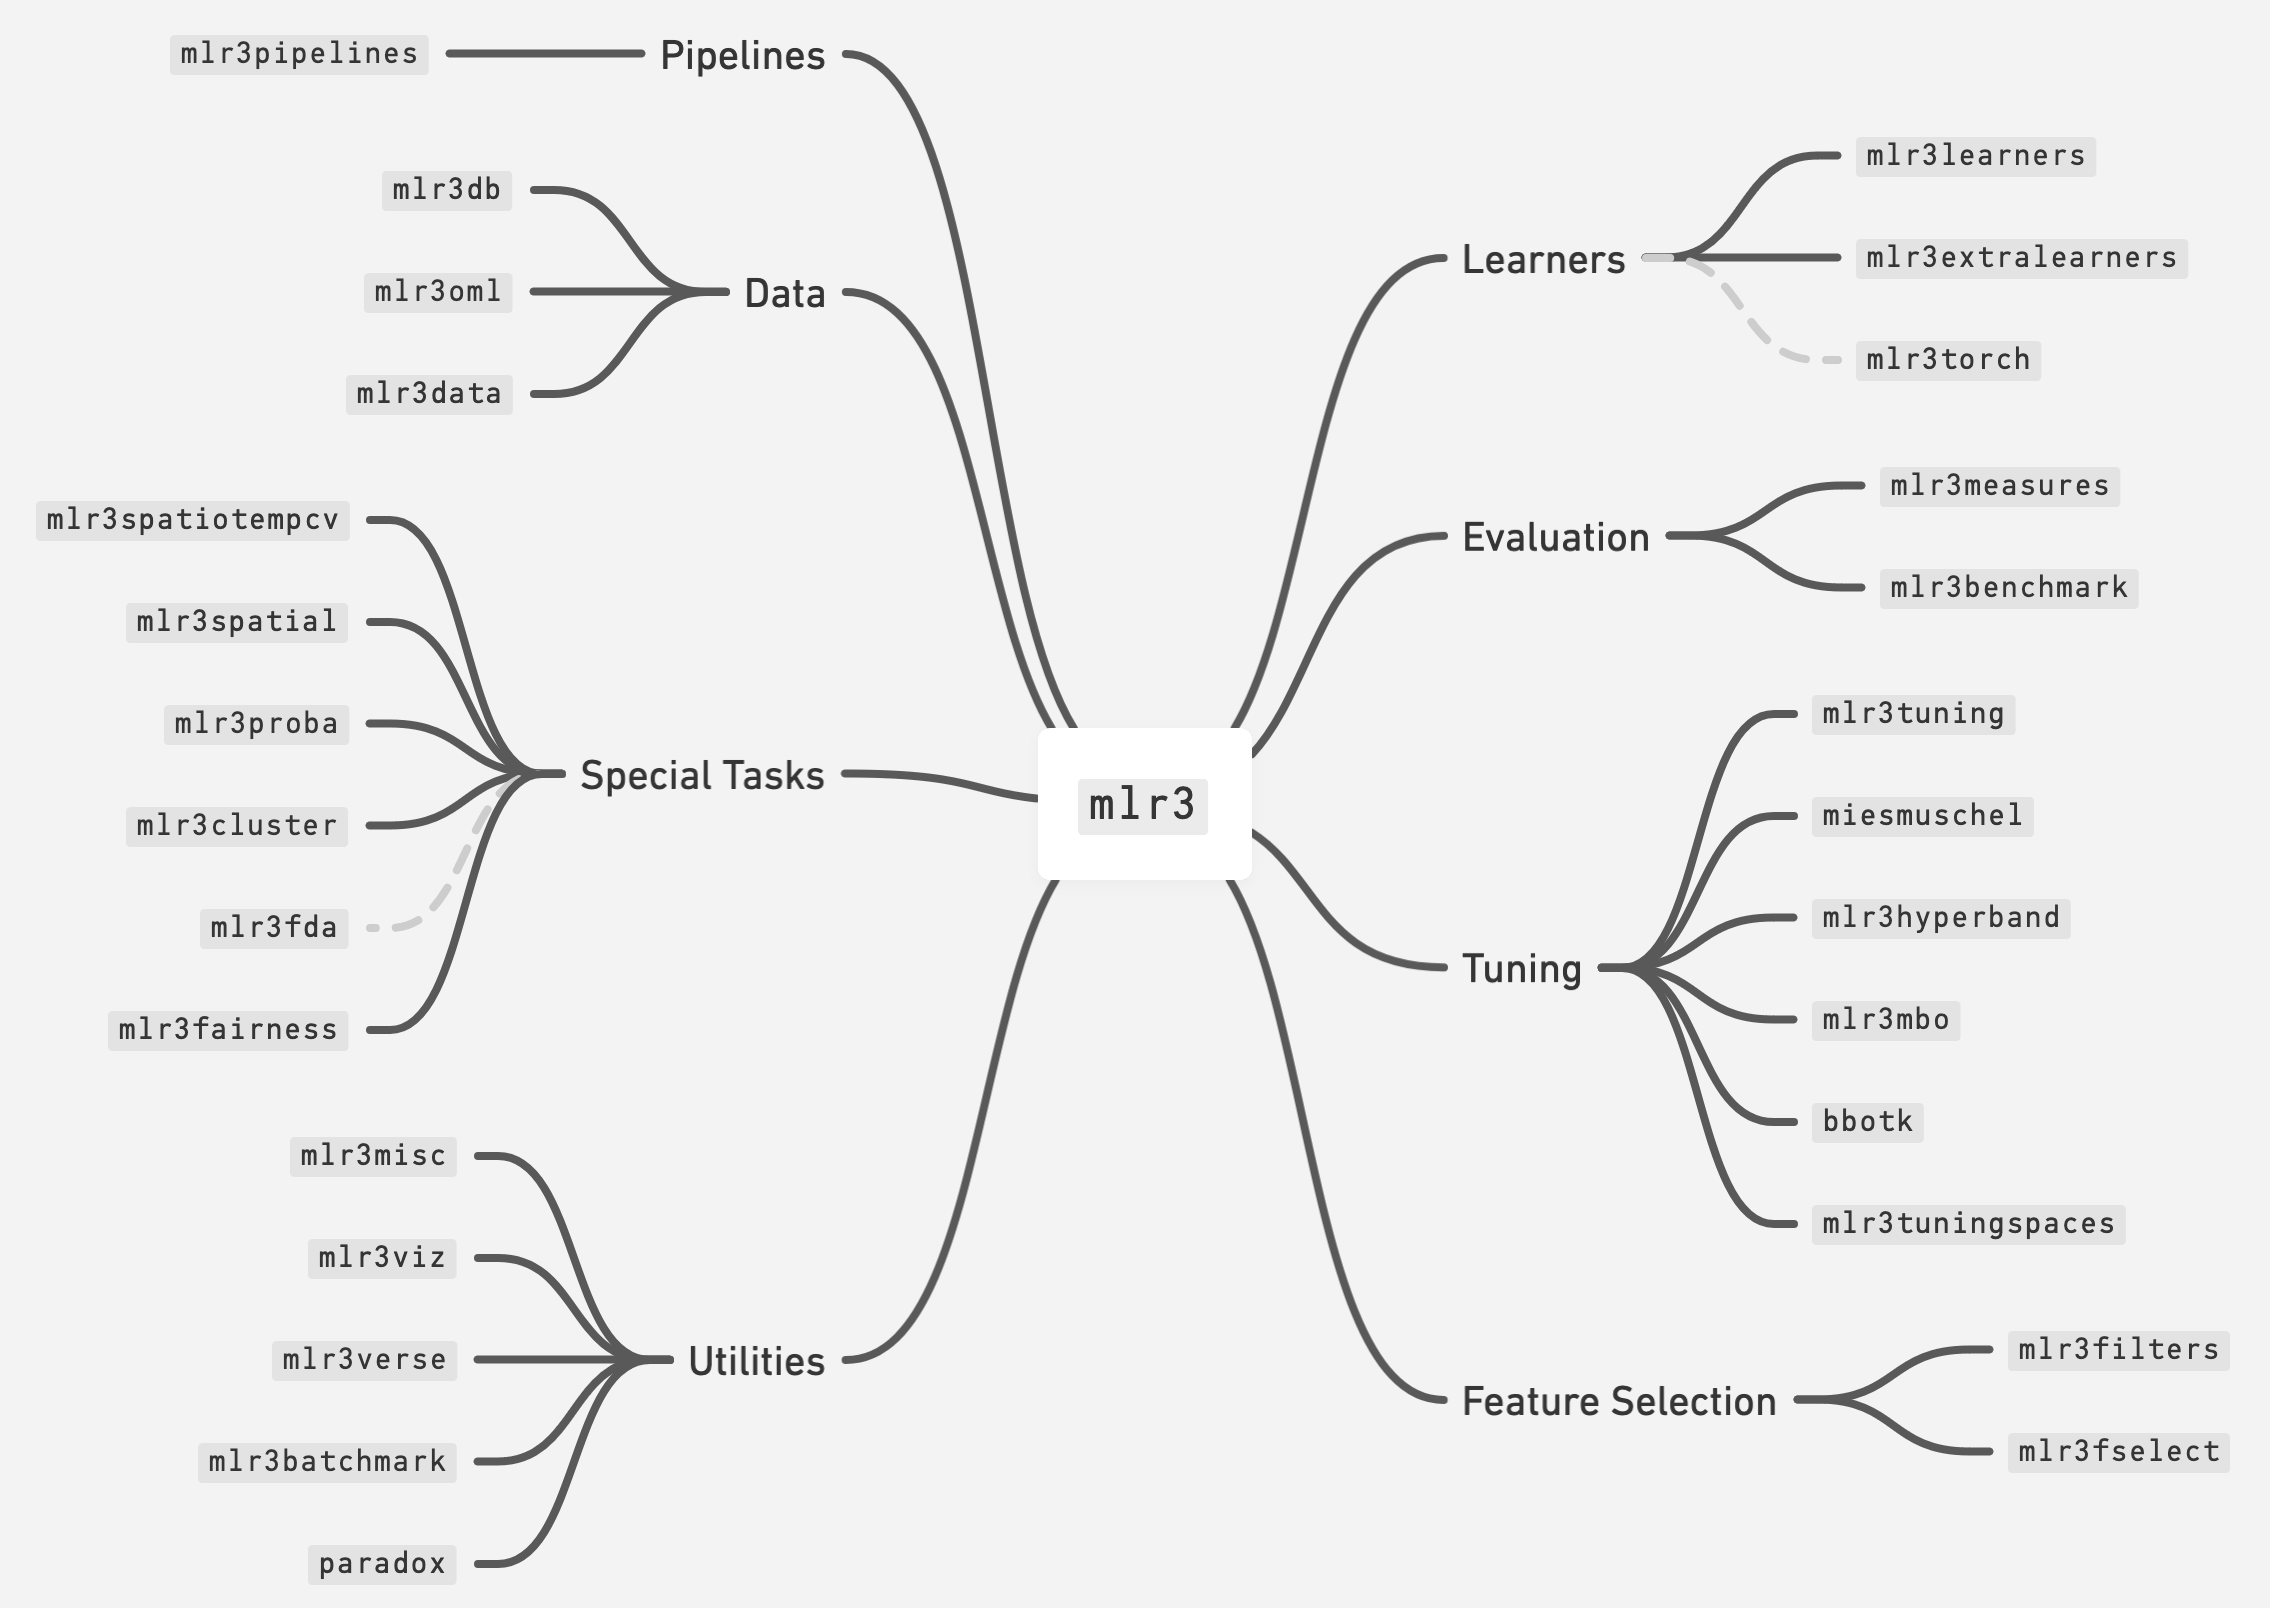
\includegraphics[width=0.8\textwidth,height=\textheight]{chapters/chapter1/Figures/mlr3_ecosystem.png}

}

\caption{\label{fig-mlr3verse}Overview of the \texttt{mlr3} ecosystem,
the packages with gray dashed lines are still in development, all others
have a stable interface.}

\end{figure}

A complete and up-to-date list of extension packages can be found at
\url{https://mlr-org.com/ecosystem.html}.

As well as packages within the \texttt{mlr3} ecosystem, software in the
\texttt{mlr3verse} also depends on the following popular and
well-established packages:

\begin{itemize}
\tightlist
\item
  \href{https://cran.r-project.org/package=R6}{\texttt{R6}}: The class
  system predominantly used in \texttt{mlr3}.
\item
  \href{https://cran.r-project.org/package=data.table}{\texttt{data.table}}:
  High-performance extension of R's \texttt{data.frame}.
\item
  \href{https://cran.r-project.org/package=digest}{\texttt{digest}}:
  Cryptographic hash functions.
\item
  \href{https://cran.r-project.org/package=uuid}{\texttt{uuid}}:
  Generation of universally unique identifiers.
\item
  \href{https://cran.r-project.org/package=lgr}{\texttt{lgr}}:
  Configurable logging library.
\item
  \href{https://cran.r-project.org/package=mlbench}{\texttt{mlbench}}
  and
  \href{https://cran.r-project.org/package=palmerpenguins}{\texttt{palmerpenguins}}:
  Machine learning datasets.
\item
  \href{https://cran.r-project.org/package=future}{\texttt{future}} /
  \href{https://cran.r-project.org/package=future.apply}{\texttt{future.apply}}
  /
  \href{https://cran.r-project.org/package=parallelly}{\texttt{parallelly}}:
  For parallelization (Section~\ref{sec-parallelization}).
\item
  \href{https://cran.r-project.org/package=evaluate}{\texttt{evaluate}}:
  For capturing output, warnings, and exceptions
  (Section~\ref{sec-error-handling}).
\end{itemize}

We build on \href{https://cran.r-project.org/package=R6}{\texttt{R6}}
for object orientation and
\href{https://cran.r-project.org/package=data.table}{\texttt{data.table}}
to store and operate on tabular data. As both are core to \texttt{mlr3}
we \emph{briefly} introduce both packages for beginners; in-depth
expertise with these packages is not necessary to work with
\texttt{mlr3}.

\hypertarget{sec-r6}{%
\subsection{R6 for Beginners}\label{sec-r6}}

\href{https://cran.r-project.org/package=R6}{\texttt{R6}} is one of R's
more recent paradigms for object-oriented
programming\index{object-oriented programming}. If you have experience
with any (class) object-oriented programming then R6 should feel
familiar. We focus on the parts of R6 that you need to know to use
\texttt{mlr3}.

\emph{Objects} are created by constructing an instance of an
\href{https://www.rdocumentation.org/packages/R6/topics/R6Class}{\texttt{R6Class}}
variable using the \texttt{\$new()} initialization method. For example,
say we have implemented a class called \texttt{Foo}, then
\texttt{foo\ =\ Foo\$new(bar\ =\ 1)} would create a new object of class
\texttt{Foo} and set the \texttt{bar} argument of the constructor to the
value \texttt{1}. In practice, we implement a lot of sugar functionality
(Section~\ref{sec-mlr3-utilities}) in \texttt{mlr3} that make
construction and access a bit more convenient.

Some \texttt{R6} objects may have mutable states that are encapsulated
in their \emph{fields}, which can be accessed through the dollar,
\texttt{\$}, operator. Continuing the previous example, we can access
the \texttt{bar} value in the \texttt{foo} object by using
\texttt{foo\$bar} or we could give it a new value,
e.g.~\texttt{foo\$bar\ =\ 2}. These fields can also be `active
bindings', which perform additional computations when referenced or
modified.

In addition to fields, \emph{methods} allow users to inspect the
object's state, retrieve information, or perform an action that changes
the internal state of the object. For example, in \texttt{mlr3}, the
\texttt{\$train()} method of a learner changes the internal state of the
learner by building and storing a model. Methods that modify the
internal state of an object often return the object itself. Other
methods may return a new R6 object. In both cases, it is possible to
`chain' methods by calling one immediately after the other using the
\texttt{\$}-operator; this is similar to the
\texttt{\%\textgreater{}\%}-operator used in \texttt{tidyverse}
packages. For example, \texttt{Foo\$bar()\$hello\_world()} would run the
\texttt{\$bar()} method of the object \texttt{Foo} and then the
\texttt{\$hello\_world()} method of the object returned by
\texttt{\$bar()} (which may be \texttt{Foo} itself).

Fields and methods can be public or private. The public fields and
methods define the API to interact with the object. In \texttt{mlr3},
you can safely ignore private methods unless you are looking to extend
our universe by adding a new class (Chapter~\ref{sec-technical}).

Finally, \texttt{R6} objects are \texttt{environments}, and as such have
reference semantics. This means that, for example, \texttt{foo2\ =\ foo}
does not create a new variable called \texttt{foo2} that is a copy of
\texttt{foo}. Instead, it creates a variable called \texttt{foo2} that
references \texttt{foo}, and so setting \texttt{foo\$bar\ =\ 3} will
also change \texttt{foo2\$bar} to \texttt{3} and vice versa. To copy an
object, use the \texttt{\$clone(deep\ =\ TRUE)} method, so to copy
\texttt{foo}:
\texttt{foo2\ =\ foo\$clone(deep\ =\ TRUE)}{\marginnote{\begin{footnotesize}\texttt{\$clone()}\end{footnotesize}}}.

For a longer introduction, we recommend the \texttt{R6} vignettes found
at \url{https://r6.r-lib.org/}; more detail can be found in
\url{https://adv-r.hadley.nz/r6.html}.

\hypertarget{sec-data.table}{%
\subsection{data.table for Beginners}\label{sec-data.table}}

The package
\href{https://cran.r-project.org/package=data.table}{\texttt{data.table}}
implements
\href{https://www.rdocumentation.org/packages/data.table/topics/data.table-package}{\texttt{data.table()}},
which is a popular alternative to R's \texttt{data.frame()}. We use
\href{https://cran.r-project.org/package=data.table}{\texttt{data.table}}
because it is blazingly fast and scales well to bigger data.

As with \texttt{data.frame}, \texttt{data.table}s can be constructed
with
\href{https://www.rdocumentation.org/packages/data.table/topics/data.table-package}{\texttt{data.table()}}
or
\href{https://www.rdocumentation.org/packages/data.table/topics/as.data.table}{\texttt{as.data.table()}}:

\begin{Shaded}
\begin{Highlighting}[]
\FunctionTok{library}\NormalTok{(data.table)}
\CommentTok{\# converting a matrix with as.data.table}
\FunctionTok{as.data.table}\NormalTok{(}\FunctionTok{matrix}\NormalTok{(}\FunctionTok{runif}\NormalTok{(}\DecValTok{4}\NormalTok{), }\DecValTok{2}\NormalTok{, }\DecValTok{2}\NormalTok{))}
\end{Highlighting}
\end{Shaded}

\begin{verbatim}
       V1     V2
1: 0.8586 0.4891
2: 0.8874 0.7181
\end{verbatim}

\begin{Shaded}
\begin{Highlighting}[]
\CommentTok{\# using data.table}
\NormalTok{dt }\OtherTok{=} \FunctionTok{data.table}\NormalTok{(}\AttributeTok{x =} \DecValTok{1}\SpecialCharTok{:}\DecValTok{6}\NormalTok{, }\AttributeTok{y =} \FunctionTok{rep}\NormalTok{(letters[}\DecValTok{1}\SpecialCharTok{:}\DecValTok{3}\NormalTok{], }\AttributeTok{each =} \DecValTok{2}\NormalTok{))}
\NormalTok{dt}
\end{Highlighting}
\end{Shaded}

\begin{verbatim}
   x y
1: 1 a
2: 2 a
3: 3 b
4: 4 b
5: 5 c
6: 6 c
\end{verbatim}

\texttt{data.table}s can be used much like \texttt{data.frame}s, but
they provide additional functionality that makes complex operations
easier. For example, data can be summarized by groups with a \texttt{by}
argument in the \texttt{{[}} operator and they can be modified in-place
with the \texttt{:=} operator.

\begin{Shaded}
\begin{Highlighting}[]
\CommentTok{\# mean of x column in groups given by y}
\NormalTok{dt[, }\FunctionTok{mean}\NormalTok{(x), by }\OtherTok{=} \StringTok{"y"}\NormalTok{]}
\end{Highlighting}
\end{Shaded}

\begin{verbatim}
   y  V1
1: a 1.5
2: b 3.5
3: c 5.5
\end{verbatim}

\begin{Shaded}
\begin{Highlighting}[]
\CommentTok{\# adding a new column with :=}
\NormalTok{dt[, z }\SpecialCharTok{:}\ErrorTok{=}\NormalTok{ x }\SpecialCharTok{*} \DecValTok{3}\NormalTok{]}
\NormalTok{dt}
\end{Highlighting}
\end{Shaded}

\begin{verbatim}
   x y  z
1: 1 a  3
2: 2 a  6
3: 3 b  9
4: 4 b 12
5: 5 c 15
6: 6 c 18
\end{verbatim}

Finally \texttt{data.table} also uses reference semantics so you will
need to use
\href{https://www.rdocumentation.org/packages/data.table/topics/copy}{\texttt{copy()}}
to clone a \texttt{data.table}. For an in-depth introduction, we
recommend the vignette {``Introduction to Data.table''} (2023).

\hypertarget{sec-mlr3-utilities}{%
\section{Essential mlr3 Utilities}\label{sec-mlr3-utilities}}

\texttt{mlr3} includes a few important utilities that are essential to
simplifying code in our ecosystem.

\hypertarget{sugar-functions}{%
\subsection*{Sugar Functions}\label{sugar-functions}}

Most objects in \texttt{mlr3} can be created through convenience
functions called helper functions or sugar
functions\index{sugar functions}. They provide shortcuts for common code
idioms, reducing the amount of code a user has to write. For example
\texttt{lrn("regr.rpart")} returns the learner without having to
explicitly create a new R6 object. We heavily use sugar functions
throughout this book and provide the equivalent ``full form'' for
complete detail at the end of each chapter. The sugar functions are
designed to cover the majority of use cases for most users, knowledge
about the full \texttt{R6} backend is only required if you want to build
custom objects or extensions.

Many object names in \texttt{mlr3} are standardized according to the
convention:
\texttt{mlr\_\textless{}type\textgreater{}\_\textless{}key\textgreater{}},
where \texttt{\textless{}type\textgreater{}} will be \texttt{tasks},
\texttt{learners}, \texttt{measures}, and other classes that will be
covered in the book, and \texttt{\textless{}key\textgreater{}} refers to
the ID of the object. To simplify the process of constructing objects,
you only need to know the object key and the sugar function for
constructing the type. For example: \texttt{mlr\_tasks\_mtcars} becomes
\texttt{tsk("mtcars")};\texttt{mlr\_learners\_regr.rpart} becomes
\texttt{lrn("regr.rpart")}; and \texttt{mlr\_measures\_regr.mse} becomes
\texttt{msr("regr.mse")}. Throughout this book, we will refer to all
objects using this abbreviated form.

\hypertarget{dictionaries}{%
\subsection*{Dictionaries}\label{dictionaries}}

\texttt{mlr3} uses dictionaries\index{dictionaries} to store R6 classes,
which associate keys (unique identifiers) with objects (R6 objects).
Values in dictionaries are often accessed through sugar functions that
retrieve objects from the relevant dictionary, for example
\texttt{lrn("regr.rpart")} is a wrapper around
\texttt{mlr\_learners\$get("regr.rpart")} and is thus a simpler way to
load a decision tree learner from
\href{https://mlr3.mlr-org.com/reference/mlr_learners.html}{\texttt{mlr\_learners}}.
We use dictionaries to group large collections of relevant objects so
they can be listed and retrieved easily. For example, you can see an
overview of available learners (that are in loaded packages) and their
properties with \texttt{as.data.table(mlr\_learners)} or by calling the
sugar function without any arguments, e.g.~\texttt{lrn()}.

\hypertarget{mlr3viz}{%
\subsection*{mlr3viz}\label{mlr3viz}}

\href{https://mlr3viz.mlr-org.com}{\texttt{mlr3viz}}\index{\texttt{mlr3viz}}
includes all plotting functionality in \texttt{mlr3} and uses
\href{https://cran.r-project.org/package=ggplot2}{\texttt{ggplot2}}
under the hood. We use
\href{https://www.rdocumentation.org/packages/ggplot2/topics/theme_minimal}{\texttt{theme\_minimal()}}
in all our plots to unify our aesthetic, but as with all \texttt{ggplot}
outputs, users can fully customize this.
\href{https://mlr3viz.mlr-org.com}{\texttt{mlr3viz}}\index{\texttt{mlr3viz}}
extends \texttt{fortify} and \texttt{autoplot} for use with common
\href{https://mlr3.mlr-org.com}{\texttt{mlr3}}\index{\texttt{mlr3}}
outputs including
\href{https://mlr3.mlr-org.com/reference/Prediction.html}{\texttt{Prediction}},
\href{https://mlr3.mlr-org.com/reference/Learner.html}{\texttt{Learner}},
and
\href{https://mlr3.mlr-org.com/reference/BenchmarkResult.html}{\texttt{BenchmarkResult}}
objects (which we will introduce and cover in the next chapters). We
will cover major plot types throughout the book. The best way to learn
about
\href{https://mlr3viz.mlr-org.com}{\texttt{mlr3viz}}\index{\texttt{mlr3viz}}
is through experimentation; load the package and see what happens when
you run \texttt{autoplot} on an \texttt{mlr3} object. Plot types are
documented in the respective manual page that can be accessed through
\texttt{?autoplot.\textless{}class\textgreater{}}, for example, you can
find different types of plots for regression tasks by running
\texttt{?autoplot.TaskRegr}.

\hypertarget{design-principles}{%
\section{Design Principles}\label{design-principles}}

\begin{tcolorbox}[enhanced jigsaw, colframe=quarto-callout-note-color-frame, rightrule=.15mm, bottomrule=.15mm, toprule=.15mm, opacityback=0, colback=white, left=2mm, arc=.35mm, breakable, leftrule=.75mm]
\begin{minipage}[t]{5.5mm}
\textcolor{quarto-callout-note-color}{\faInfo}
\end{minipage}%
\begin{minipage}[t]{\textwidth - 5.5mm}

\textbf{This section covers advanced ML or technical
details.}\vspace{2mm}

\end{minipage}%
\end{tcolorbox}

The
\href{https://cran.r-project.org/package=mlr}{\texttt{mlr}}\index{\texttt{mlr}}
package (Bischl et al. 2016) was first released on CRAN in 2013, with
the core design and architecture dating back further. Over time, the
addition of many features led to a complex design that made it too
difficult for us to extend further. In hindsight, we saw that some
design and architecture choices in
\href{https://cran.r-project.org/package=mlr}{\texttt{mlr}} made it
difficult to support new features, in particular with respect to ML
pipelines. So in 2018, we set about working on a reimplementation, which
resulted in the first release of
\href{https://mlr3.mlr-org.com}{\texttt{mlr3}}\index{\texttt{mlr3}} on
CRAN in July 2019.

Learning from our history, we now follow these design principles in the
\texttt{mlr3} ecosystem:

\begin{itemize}
\tightlist
\item
  \textbf{Object-oriented programming}. We embrace
  \href{https://cran.r-project.org/package=R6}{\texttt{R6}} for a clean,
  object-oriented design, object state changes, and reference semantics.
  This means that the state of common objects (e.g.~tasks
  (Section~\ref{sec-tasks}) and learners (Section~\ref{sec-learners}))
  is encapsulated within the object, for example, to keep track of
  whether a model has been trained, without the user having to worry
  about this. We also use inheritance to specialize objects, e.g.~all
  learners are derived from a common base class that provides basic
  functionality.
\item
  \textbf{Tabular data}. Embrace
  \href{https://cran.r-project.org/package=data.table}{\texttt{data.table}}
  for its top-notch computational performance as well as tabular data as
  a structure that can be easily processed further.
\item
  \textbf{Unified tabular input and output data formats.} This
  considerably simplifies the API and allows easy selection and
  ``split-apply-combine'' (aggregation) operations. We combine
  \texttt{data.table} and \texttt{R6} to place references to non-atomic
  and compound objects in tables and make heavy use of list columns.
\item
  \textbf{Defensive programming and type safety}. All user input is
  checked with
  \href{https://cran.r-project.org/package=checkmate}{\texttt{checkmate}}
  (Lang 2017). We use \texttt{data.table}, which has behavior that is
  more consistent than several base R methods (e.g., indexing
  \texttt{data.frame}s simplifies the result when the \texttt{drop}
  argument is omitted). And we have extensive unit tests!
\item
  \textbf{Light on dependencies}. One of the main maintenance burdens
  for \href{https://cran.r-project.org/package=mlr}{\texttt{mlr}} was to
  keep up with changing learner interfaces and behavior of the many
  packages it depended on. We require far fewer packages in
  \href{https://mlr3.mlr-org.com}{\texttt{mlr3}}\index{\texttt{mlr3}},
  which makes installation and maintenance easier. We still provide the
  same functionality, but it is split into more packages that have fewer
  dependencies individually.
\item
  \textbf{Separation of computation and presentation}. Most packages of
  the
  \href{https://mlr3.mlr-org.com}{\texttt{mlr3}}\index{\texttt{mlr3}}
  ecosystem focus on processing and transforming data, applying ML
  algorithms, and computing results. Our core packages do not provide
  visualizations because their dependencies would make installation
  unnecessarily complex, especially on headless servers (i.e., computers
  without a monitor where graphical libraries are not installed). Hence,
  visualizations of data and results are provided in
  \href{https://mlr3viz.mlr-org.com}{\texttt{mlr3viz}}\index{\texttt{mlr3viz}}.
\end{itemize}



\part{Fundamentals}

\hypertarget{sec-basics}{%
\chapter{Data and Basic Modeling}\label{sec-basics}}

\vspace{-15mm}\addtocontents{toc}{\textit{Natalie Foss and Lars Kotthoff}}

\textbf{Natalie Foss} \newline  \emph{University of Wyoming}

\textbf{Lars Kotthoff} \newline  \emph{University of Wyoming}
\newline \newline 

In this chapter, we will introduce the
\href{https://mlr3.mlr-org.com}{\texttt{mlr3}}\index{\texttt{mlr3}}
objects and corresponding
\href{https://cran.r-project.org/package=R6}{\texttt{R6}} classes that
implement the essential building blocks of machine learning. These
building blocks include the data (and the methods for creating training
and test sets), the machine learning algorithm\index{algorithm} (and its
training and prediction process), the configuration of a machine
learning algorithm through its hyperparameters\index{hyperparameters},
and evaluation measures to assess the quality of predictions.

In the simplest definition, machine learning\index{machine learning}
(ML) is the process of learning models of relationships from
data.{\marginnote{\begin{footnotesize}Machine Learning/Supervised
Learning\end{footnotesize}}} Supervised
learning\index{supervised learning} is a subfield of ML in which
datasets consist of labeled observations, which means that each data
point consists of features\index{features}, which are variables to make
predictions from, and a target\index{target}, which is the quantity that
we are trying to predict. For example, predicting a car's miles per
gallon (target) based on the car's properties (features) such as
horsepower and the number of gears is a supervised learning problem,
which we will return to several times in this book. In \texttt{mlr3}, we
refer to datasets, and their associated metadata as tasks\index{tasks}
(Section~\ref{sec-tasks}). The term `task' is used to refer to the
prediction problem that we are trying to solve. Tasks are defined by the
features used for prediction and the targets to predict, so there can be
multiple tasks associated with any given dataset. For example,
predicting miles per gallon (mpg) from horsepower is one task,
predicting horsepower from mpg is another task, and predicting the
number of gears from the car's model is yet another task.

Supervised learning can be further divided into
regression\index{regression}{\marginnote{\begin{footnotesize}Regression\end{footnotesize}}}
-- which is the prediction of numeric target values, e.g.~predicting a
car's mpg -- and
classification\index{classification}{\marginnote{\begin{footnotesize}Classification\end{footnotesize}}}
-- which is the prediction of categorical values/labels, e.g.,
predicting a car's model. Chapter~\ref{sec-special} also discusses other
tasks, including cost-sensitive
classification\index{classification!cost-sensitive} and unsupervised
learning\index{unsupervised learning}. For any supervised learning task,
the goal is to build a model\index{model} that captures the relationship
between the features and target, often with the goal of
training\index{model training} the model to learn relationships about
the data so it can make predictions for new and previously unseen data.
A
model\index{model}{\marginnote{\begin{footnotesize}Model\end{footnotesize}}}
is formally a mapping from a feature vector to a prediction. A
prediction can take many forms depending on the task; for example, in
classification this can be a predicted label, or a set of predicted
probabilities or scores. Models are induced by passing training
data\index{training data} to machine learning algorithms, such as
decision trees\index{decision tree}, support vector
machines\index{support vector machine}, neural
networks\index{neural network}, and many more. Machine learning
algorithms are called
learners{\marginnote{\begin{footnotesize}Learners\end{footnotesize}}} in
\texttt{mlr3} (Section~\ref{sec-learners}) as, given data, they learn
models. Each learner has a parameterized space that potential models are
drawn from and during the training process, these parameters are fitted
to best match the data. For example, the parameters could be the
coefficients used for individual features when training a linear
regression model. During training, most machine learning algorithms are
`fitted'/`trained'\index{model training}\index{fitting|see{model training}}
by optimizing a loss-function that quantifies the mismatch between
ground truth target values in the training data and the predictions of
the model.

For a model to be most useful, it should generalize beyond the training
data to make `good' predictions (Section~\ref{sec-predicting}) on new
and previously `unseen' (by the model) data. The simplest way to test
this, is to split data into training data\index{training data} and test
data\index{test data}{\marginnote{\begin{footnotesize}Train/Test
Data\end{footnotesize}}} -- where the model is trained on the training
data and then the separate test data is used to evaluate models in an
unbiased way by assessing to what extent the model has learned the true
relationships that underlie the data (Chapter~\ref{sec-performance}).
This evaluation procedure estimates a model's generalization
error\index{generalization error}{\marginnote{\begin{footnotesize}Generalization
Error\end{footnotesize}}}, i.e., how well we expect the model to perform
in general. There are many ways to evaluate models and to split data for
estimating generalization error (Section~\ref{sec-resampling}).

This brief overview of ML provides the basic knowledge required to use
\texttt{mlr3} and is summarized in
Figure~\ref{fig-ml-abstraction-basics}. In the rest of this book, we
will provide introductions to methodology when relevant. For texts about
ML, including detailed methodology and underpinnings of different
algorithms, we recommend Hastie, Friedman, and Tibshirani (2001), James
et al. (2014), and Bishop (2006).

In the next few sections we will look at the building blocks of
\texttt{mlr3} using regression as an example, we will then consider how
to extend this to classification in Section~\ref{sec-classif}.

\begin{figure}

{\centering 
\includegraphics[width=1\textwidth,height=\textheight]{chapters/chapter2/Figures/mlr3book_figures-1.png}

}

\caption{\label{fig-ml-abstraction-basics}General overview of the
machine learning process.}

\end{figure}

\hypertarget{sec-tasks}{%
\section{Tasks}\label{sec-tasks}}

Tasks\index{tasks} are objects that contain the (usually tabular) data
and additional metadata that define a machine learning problem. The
metadata\index{metadata} contain, for example, the name of the target
feature for supervised machine learning problems. This information is
extracted automatically when required, so the user does not have to
specify the prediction target every time a model is trained.

\hypertarget{sec-tasks-built-in}{%
\subsection{Constructing Tasks}\label{sec-tasks-built-in}}

\texttt{mlr3} includes a few predefined machine learning tasks in the
\href{https://mlr3.mlr-org.com/reference/mlr_tasks.html}{\texttt{mlr\_tasks}}\index{\texttt{mlr\_tasks}}{\marginnote{\begin{footnotesize}\texttt{mlr\_tasks}\end{footnotesize}}}
\texttt{Dictionary}.

\begin{Shaded}
\begin{Highlighting}[]
\NormalTok{mlr\_tasks}
\end{Highlighting}
\end{Shaded}

\begin{verbatim}
<DictionaryTask> with 21 stored values
Keys: ames_housing, bike_sharing, boston_housing, breast_cancer,
  german_credit, ilpd, iris, kc_housing, moneyball, mtcars,
  optdigits, penguins, penguins_simple, pima, ruspini, sonar,
  spam, titanic, usarrests, wine, zoo
\end{verbatim}

To get a task from the dictionary, use the
\href{https://mlr3.mlr-org.com/reference/mlr_sugar.html}{\texttt{tsk()}}\index{\texttt{tsk()}}{\marginnote{\begin{footnotesize}\texttt{tsk()}\end{footnotesize}}}
function and assign the return value to a new variable. Below we
retrieve \texttt{tsk("mtcars")}, which uses the
\href{https://www.rdocumentation.org/packages/datasets/topics/mtcars}{\texttt{mtcars}}
dataset:

\begin{Shaded}
\begin{Highlighting}[]
\NormalTok{tsk\_mtcars }\OtherTok{=} \FunctionTok{tsk}\NormalTok{(}\StringTok{"mtcars"}\NormalTok{)}
\NormalTok{tsk\_mtcars}
\end{Highlighting}
\end{Shaded}

\begin{verbatim}
<TaskRegr:mtcars> (32 x 11): Motor Trends
* Target: mpg
* Properties: -
* Features (10):
  - dbl (10): am, carb, cyl, disp, drat, gear, hp, qsec, vs, wt
\end{verbatim}

Running \texttt{tsk()} without any arguments will list all the tasks in
the dictionary, this also works for all other sugar constructors that
you will encounter throughout the book.

\begin{tcolorbox}[enhanced jigsaw, opacitybacktitle=0.6, rightrule=.15mm, opacityback=0, arc=.35mm, breakable, titlerule=0mm, colframe=quarto-callout-tip-color-frame, coltitle=black, bottomrule=.15mm, toprule=.15mm, colback=white, colbacktitle=quarto-callout-tip-color!10!white, bottomtitle=1mm, toptitle=1mm, title=\textcolor{quarto-callout-tip-color}{\faLightbulb}\hspace{0.5em}{Help Pages}, leftrule=.75mm, left=2mm]

Usually in R, the help pages of functions can be queried with
\texttt{?}. The same is true of R6 classes, so if you want to find the
help page of the \texttt{mtcars} task you could use
\texttt{?mlr\_tasks\_mtcars}. We have also added a \texttt{\$help()}
method to many of our classes, which allows you to access the help page
from any instance of that class, for example:
\texttt{tsk("mtcars")\$help()}.

\end{tcolorbox}

To create your own regression task, you will need to construct a new
instance of
\href{https://mlr3.mlr-org.com/reference/TaskRegr.html}{\texttt{TaskRegr}}\index{\texttt{TaskRegr}}{\marginnote{\begin{footnotesize}\texttt{TaskRegr}\end{footnotesize}}}.
The simplest way to do this is with the function
\href{https://mlr3.mlr-org.com/reference/as_task_regr.html}{\texttt{as\_task\_regr()}}\index{\texttt{as\_task\_regr()}}{\marginnote{\begin{footnotesize}\texttt{as\_task\_regr()}\end{footnotesize}}}
to convert a \texttt{data.frame} type object to a regression task,
specifying the target feature by passing this to the \texttt{target}
argument. By example, we will ignore that \texttt{mtcars} is already
available as a predefined task in \texttt{mlr3}. In the code below we
load the \texttt{datasets::mtcars} dataset, subset the data to only
include columns \texttt{"mpg"}, \texttt{"cyl"}, \texttt{"disp"}, print
the modified data's properties, and then set up a regression task called
\texttt{"cars"} (\texttt{id\ =\ "cars"}) in which we will try to predict
miles per gallon (\texttt{target\ =\ "mpg"}) from the number of
cylinders (\texttt{"cyl"}) and displacement (\texttt{"disp"}):

\begin{Shaded}
\begin{Highlighting}[]
\FunctionTok{data}\NormalTok{(}\StringTok{"mtcars"}\NormalTok{, }\AttributeTok{package =} \StringTok{"datasets"}\NormalTok{)}
\NormalTok{mtcars\_subset }\OtherTok{=} \FunctionTok{subset}\NormalTok{(mtcars, }\AttributeTok{select =} \FunctionTok{c}\NormalTok{(}\StringTok{"mpg"}\NormalTok{, }\StringTok{"cyl"}\NormalTok{, }\StringTok{"disp"}\NormalTok{))}
\FunctionTok{str}\NormalTok{(mtcars\_subset)}
\end{Highlighting}
\end{Shaded}

\begin{verbatim}
'data.frame':   32 obs. of  3 variables:
 $ mpg : num  21 21 22.8 21.4 18.7 18.1 14.3 24.4 22.8 19.2 ...
 $ cyl : num  6 6 4 6 8 6 8 4 4 6 ...
 $ disp: num  160 160 108 258 360 ...
\end{verbatim}

\begin{Shaded}
\begin{Highlighting}[]
\NormalTok{tsk\_mtcars }\OtherTok{=} \FunctionTok{as\_task\_regr}\NormalTok{(mtcars\_subset, }\AttributeTok{target =} \StringTok{"mpg"}\NormalTok{, }\AttributeTok{id =} \StringTok{"cars"}\NormalTok{)}
\end{Highlighting}
\end{Shaded}

The data can be in any tabular format, e.g.~a \texttt{data.frame()},
\texttt{data.table()}, or \texttt{tibble()}. The \texttt{target}
argument specifies the prediction target column. The \texttt{id}
argument is optional and specifies an identifier for the task that is
used in plots and summaries; if omitted the variable name of the data
will be used as the \texttt{id}.

\begin{tcolorbox}[enhanced jigsaw, opacitybacktitle=0.6, rightrule=.15mm, opacityback=0, arc=.35mm, breakable, titlerule=0mm, colframe=quarto-callout-tip-color-frame, coltitle=black, bottomrule=.15mm, toprule=.15mm, colback=white, colbacktitle=quarto-callout-tip-color!10!white, bottomtitle=1mm, toptitle=1mm, title=\textcolor{quarto-callout-tip-color}{\faLightbulb}\hspace{0.5em}{UTF8 Column Names}, leftrule=.75mm, left=2mm]

As many machine learning models do not work properly with arbitrary UTF8
names, \texttt{mlr3} defaults to throwing an error if any of the column
names passed to
\href{https://mlr3.mlr-org.com/reference/as_task_regr.html}{\texttt{as\_task\_regr()}}
(and other task constructors) contain a non-ASCII character or do not
comply with R's variable naming scheme. Therefore, we recommend
converting names with
\href{https://www.rdocumentation.org/packages/base/topics/make.names}{\texttt{make.names()}}
if possible. You can bypass this check by setting
\texttt{options(mlr3.allow\_utf8\_names\ =\ TRUE)} (but do not be
surprised if errors occur later, especially when passing objects to
other packages).

\end{tcolorbox}

Printing a task provides a summary and in this case, we can see the task
has 32 observations and 3 columns (32 x 3), of which \texttt{mpg} is the
target, there are no special properties (\texttt{Properties:\ -}), and
there are 2 features stored in double-precision floating point format.

\begin{Shaded}
\begin{Highlighting}[]
\NormalTok{tsk\_mtcars}
\end{Highlighting}
\end{Shaded}

\begin{verbatim}
<TaskRegr:cars> (32 x 3)
* Target: mpg
* Properties: -
* Features (2):
  - dbl (2): cyl, disp
\end{verbatim}

We can plot the task using the
\href{https://mlr3viz.mlr-org.com}{\texttt{mlr3viz}}\index{\texttt{mlr3viz}}
package, which gives a graphical summary of the distribution of the
target and feature values:

\begin{Shaded}
\begin{Highlighting}[]
\FunctionTok{library}\NormalTok{(mlr3viz)}
\FunctionTok{autoplot}\NormalTok{(tsk\_mtcars, }\AttributeTok{type =} \StringTok{"pairs"}\NormalTok{)}
\end{Highlighting}
\end{Shaded}

\hypertarget{sec-retrieve-data}{%
\subsection{Retrieving Data}\label{sec-retrieve-data}}

We have looked at how to create tasks to store data and metadata, now we
will look at how to retrieve the stored data.

Various fields can be used to retrieve metadata about a task. The
dimensions, for example, can be retrieved using \texttt{\$nrow} and
\texttt{\$ncol}:

\begin{Shaded}
\begin{Highlighting}[]
\FunctionTok{c}\NormalTok{(tsk\_mtcars}\SpecialCharTok{$}\NormalTok{nrow, tsk\_mtcars}\SpecialCharTok{$}\NormalTok{ncol)}
\end{Highlighting}
\end{Shaded}

\begin{verbatim}
[1] 32  3
\end{verbatim}

The names of the feature and target columns are stored in the
\texttt{\$feature\_names} and \texttt{\$target\_names} slots,
respectively.

\begin{Shaded}
\begin{Highlighting}[]
\FunctionTok{c}\NormalTok{(}\AttributeTok{Features =}\NormalTok{ tsk\_mtcars}\SpecialCharTok{$}\NormalTok{feature\_names,}
  \AttributeTok{Target =}\NormalTok{ tsk\_mtcars}\SpecialCharTok{$}\NormalTok{target\_names)}
\end{Highlighting}
\end{Shaded}

\begin{verbatim}
Features1 Features2    Target 
    "cyl"    "disp"     "mpg" 
\end{verbatim}

The columns of a task have unique \texttt{character}-valued names and
the rows are identified by unique natural numbers, called row IDs. They
can be accessed through the \texttt{\$row\_ids} field:

\begin{Shaded}
\begin{Highlighting}[]
\FunctionTok{head}\NormalTok{(tsk\_mtcars}\SpecialCharTok{$}\NormalTok{row\_ids)}
\end{Highlighting}
\end{Shaded}

\begin{verbatim}
[1] 1 2 3 4 5 6
\end{verbatim}

Row IDs are not used as features when training or predicting but are
metadata that allow access to individual observations. Note that row IDs
are not the same as row numbers. This is best demonstrated by example,
below we create a regression task from random data, print the original
row IDs, which correspond to row numbers 1-5, then we filter three rows
(we will return to this method just below) and print the new row IDs,
which no longer correspond to the row numbers.

\begin{Shaded}
\begin{Highlighting}[]
\NormalTok{task }\OtherTok{=} \FunctionTok{as\_task\_regr}\NormalTok{(}\FunctionTok{data.frame}\NormalTok{(}\AttributeTok{x =} \FunctionTok{runif}\NormalTok{(}\DecValTok{5}\NormalTok{), }\AttributeTok{y =} \FunctionTok{runif}\NormalTok{(}\DecValTok{5}\NormalTok{)),}
  \AttributeTok{target =} \StringTok{"y"}\NormalTok{)}
\NormalTok{task}\SpecialCharTok{$}\NormalTok{row\_ids}
\end{Highlighting}
\end{Shaded}

\begin{verbatim}
[1] 1 2 3 4 5
\end{verbatim}

\begin{Shaded}
\begin{Highlighting}[]
\NormalTok{task}\SpecialCharTok{$}\FunctionTok{filter}\NormalTok{(}\FunctionTok{c}\NormalTok{(}\DecValTok{4}\NormalTok{, }\DecValTok{1}\NormalTok{, }\DecValTok{3}\NormalTok{))}
\NormalTok{task}\SpecialCharTok{$}\NormalTok{row\_ids}
\end{Highlighting}
\end{Shaded}

\begin{verbatim}
[1] 1 3 4
\end{verbatim}

This design decision allows tasks and learners to transparently operate
on real database management systems, where primary keys are required to
be unique, but not necessarily consecutive. See
Section~\ref{sec-backends} for more information on using databases as
data backends for tasks

The data contained in a task can be accessed through \texttt{\$data()},
which returns a
\href{https://www.rdocumentation.org/packages/data.table/topics/data.table-package}{\texttt{data.table}}
object. This method has optional \texttt{rows} and \texttt{cols}
arguments to specify subsets of the data to retrieve.

\begin{Shaded}
\begin{Highlighting}[]
\CommentTok{\# retrieve all data}
\NormalTok{tsk\_mtcars}\SpecialCharTok{$}\FunctionTok{data}\NormalTok{()}
\end{Highlighting}
\end{Shaded}

\begin{verbatim}
     mpg cyl  disp
 1: 21.0   6 160.0
 2: 21.0   6 160.0
 3: 22.8   4 108.0
 4: 21.4   6 258.0
 5: 18.7   8 360.0
---               
28: 30.4   4  95.1
29: 15.8   8 351.0
30: 19.7   6 145.0
31: 15.0   8 301.0
32: 21.4   4 121.0
\end{verbatim}

\begin{Shaded}
\begin{Highlighting}[]
\CommentTok{\# retrieve data for rows with IDs 1, 5, and 10 and all feature columns}
\NormalTok{tsk\_mtcars}\SpecialCharTok{$}\FunctionTok{data}\NormalTok{(}\AttributeTok{rows =} \FunctionTok{c}\NormalTok{(}\DecValTok{1}\NormalTok{, }\DecValTok{5}\NormalTok{, }\DecValTok{10}\NormalTok{), }\AttributeTok{cols =}\NormalTok{ tsk\_mtcars}\SpecialCharTok{$}\NormalTok{feature\_names)}
\end{Highlighting}
\end{Shaded}

\begin{verbatim}
   cyl  disp
1:   6 160.0
2:   8 360.0
3:   6 167.6
\end{verbatim}

\begin{tcolorbox}[enhanced jigsaw, opacitybacktitle=0.6, rightrule=.15mm, opacityback=0, arc=.35mm, breakable, titlerule=0mm, colframe=quarto-callout-tip-color-frame, coltitle=black, bottomrule=.15mm, toprule=.15mm, colback=white, colbacktitle=quarto-callout-tip-color!10!white, bottomtitle=1mm, toptitle=1mm, title=\textcolor{quarto-callout-tip-color}{\faLightbulb}\hspace{0.5em}{Accessing Rows by Number}, leftrule=.75mm, left=2mm]

You can work with row numbers instead of row IDs by using the
\texttt{\$row\_ids} field to extract the row ID corresponding to a given
row number:

\begin{Shaded}
\begin{Highlighting}[]
\CommentTok{\# select the 2nd row of the task by extracting the second row\_id:}
\NormalTok{tsk\_mtcars}\SpecialCharTok{$}\FunctionTok{data}\NormalTok{(}\AttributeTok{rows =}\NormalTok{ task}\SpecialCharTok{$}\NormalTok{row\_ids[}\DecValTok{2}\NormalTok{])}
\end{Highlighting}
\end{Shaded}

\end{tcolorbox}

You can always use `standard' R methods to extract summary data from a
task, for example, to summarize the underlying data:

\begin{Shaded}
\begin{Highlighting}[]
\FunctionTok{summary}\NormalTok{(}\FunctionTok{as.data.table}\NormalTok{(tsk\_mtcars))}
\end{Highlighting}
\end{Shaded}

\begin{verbatim}
      mpg            cyl            disp      
 Min.   :10.4   Min.   :4.00   Min.   : 71.1  
 1st Qu.:15.4   1st Qu.:4.00   1st Qu.:120.8  
 Median :19.2   Median :6.00   Median :196.3  
 Mean   :20.1   Mean   :6.19   Mean   :230.7  
 3rd Qu.:22.8   3rd Qu.:8.00   3rd Qu.:326.0  
 Max.   :33.9   Max.   :8.00   Max.   :472.0  
\end{verbatim}

\hypertarget{sec-tasks-mutators}{%
\subsection{Task Mutators}\label{sec-tasks-mutators}}

After a task has been created, you may want to perform operations on the
task such as filtering down to subsets of rows and columns, which is
often useful for manually creating train and test splits or to fit
models on a subset of given features. Above we saw how to access subsets
of the underlying dataset using \texttt{\$data()}, however, this will
not change the underlying task. Therefore, we provide
mutators\index{mutators}{\marginnote{\begin{footnotesize}Mutators\end{footnotesize}}},
which modify the given \texttt{Task} in place, which can be seen in the
examples below.

Subsetting by features (columns) is possible with \texttt{\$select()}
with the desired feature names passed as a character vector and
subsetting by observations (rows) is performed with \texttt{\$filter()}
by passing the row IDs as a numeric vector.
\index{\texttt{Task}!\texttt{\$select()}}
\index{\texttt{Task}!\texttt{\$filter()}}

\begin{Shaded}
\begin{Highlighting}[]
\NormalTok{tsk\_mtcars\_small }\OtherTok{=} \FunctionTok{tsk}\NormalTok{(}\StringTok{"mtcars"}\NormalTok{) }\CommentTok{\# initialize with the full task}
\NormalTok{tsk\_mtcars\_small}\SpecialCharTok{$}\FunctionTok{select}\NormalTok{(}\StringTok{"cyl"}\NormalTok{) }\CommentTok{\# keep only one feature}
\NormalTok{tsk\_mtcars\_small}\SpecialCharTok{$}\FunctionTok{filter}\NormalTok{(}\DecValTok{2}\SpecialCharTok{:}\DecValTok{3}\NormalTok{) }\CommentTok{\# keep only these rows}
\NormalTok{tsk\_mtcars\_small}\SpecialCharTok{$}\FunctionTok{data}\NormalTok{()}
\end{Highlighting}
\end{Shaded}

\begin{verbatim}
    mpg cyl
1: 21.0   6
2: 22.8   4
\end{verbatim}

As \texttt{R6} uses reference semantics (Section~\ref{sec-r6}), you need
to use \texttt{\$clone()} if you want to modify a task while keeping the
original object intact.

\begin{Shaded}
\begin{Highlighting}[]
\CommentTok{\# the wrong way}
\NormalTok{tsk\_mtcars }\OtherTok{=} \FunctionTok{tsk}\NormalTok{(}\StringTok{"mtcars"}\NormalTok{)}
\NormalTok{tsk\_mtcars\_wrong }\OtherTok{=}\NormalTok{ tsk\_mtcars}
\NormalTok{tsk\_mtcars\_wrong}\SpecialCharTok{$}\FunctionTok{filter}\NormalTok{(}\DecValTok{1}\SpecialCharTok{:}\DecValTok{2}\NormalTok{)}
\CommentTok{\# original data affected}
\NormalTok{tsk\_mtcars}\SpecialCharTok{$}\FunctionTok{head}\NormalTok{()}
\end{Highlighting}
\end{Shaded}

\begin{verbatim}
   mpg am carb cyl disp drat gear  hp  qsec vs    wt
1:  21  1    4   6  160  3.9    4 110 16.46  0 2.620
2:  21  1    4   6  160  3.9    4 110 17.02  0 2.875
\end{verbatim}

\begin{Shaded}
\begin{Highlighting}[]
\CommentTok{\# the right way}
\NormalTok{tsk\_mtcars }\OtherTok{=} \FunctionTok{tsk}\NormalTok{(}\StringTok{"mtcars"}\NormalTok{)}
\NormalTok{tsk\_mtcars\_right }\OtherTok{=}\NormalTok{ tsk\_mtcars}\SpecialCharTok{$}\FunctionTok{clone}\NormalTok{()}
\NormalTok{tsk\_mtcars\_right}\SpecialCharTok{$}\FunctionTok{filter}\NormalTok{(}\DecValTok{1}\SpecialCharTok{:}\DecValTok{2}\NormalTok{)}
\CommentTok{\# original data unaffected}
\NormalTok{tsk\_mtcars}\SpecialCharTok{$}\FunctionTok{head}\NormalTok{()}
\end{Highlighting}
\end{Shaded}

\begin{verbatim}
    mpg am carb cyl disp drat gear  hp  qsec vs    wt
1: 21.0  1    4   6  160 3.90    4 110 16.46  0 2.620
2: 21.0  1    4   6  160 3.90    4 110 17.02  0 2.875
3: 22.8  1    1   4  108 3.85    4  93 18.61  1 2.320
4: 21.4  0    1   6  258 3.08    3 110 19.44  1 3.215
5: 18.7  0    2   8  360 3.15    3 175 17.02  0 3.440
6: 18.1  0    1   6  225 2.76    3 105 20.22  1 3.460
\end{verbatim}

To add extra rows and columns to a task, you can use \texttt{\$rbind()}
and \texttt{\$cbind()} respectively:
\index{\texttt{Task}!\texttt{\$cbind()}}
\index{\texttt{Task}!\texttt{\$rbind()}}

\begin{Shaded}
\begin{Highlighting}[]
\NormalTok{tsk\_mtcars\_small}\SpecialCharTok{$}\FunctionTok{cbind}\NormalTok{( }\CommentTok{\# add another column}
  \FunctionTok{data.frame}\NormalTok{(}\AttributeTok{disp =} \FunctionTok{c}\NormalTok{(}\DecValTok{150}\NormalTok{, }\DecValTok{160}\NormalTok{))}
\NormalTok{)}
\NormalTok{tsk\_mtcars\_small}\SpecialCharTok{$}\FunctionTok{rbind}\NormalTok{( }\CommentTok{\# add another row}
  \FunctionTok{data.frame}\NormalTok{(}\AttributeTok{mpg =} \DecValTok{23}\NormalTok{, }\AttributeTok{cyl =} \DecValTok{5}\NormalTok{, }\AttributeTok{disp =} \DecValTok{170}\NormalTok{)}
\NormalTok{)}
\NormalTok{tsk\_mtcars\_small}\SpecialCharTok{$}\FunctionTok{data}\NormalTok{()}
\end{Highlighting}
\end{Shaded}

\begin{verbatim}
    mpg cyl disp
1: 21.0   6  150
2: 22.8   4  160
3: 23.0   5  170
\end{verbatim}

\hypertarget{sec-learners}{%
\section{Learners}\label{sec-learners}}

Objects of class
\href{https://mlr3.mlr-org.com/reference/Learner.html}{\texttt{Learner}}\index{\texttt{Learner}}{\marginnote{\begin{footnotesize}\texttt{Learner}\end{footnotesize}}}
provide a unified interface to many popular machine learning algorithms
in R. The
\href{https://mlr3.mlr-org.com/reference/mlr_learners.html}{\texttt{mlr\_learners}}\index{\texttt{mlr\_learners}}{\marginnote{\begin{footnotesize}\texttt{mlr\_learners}\end{footnotesize}}}
dictionary contains all the learners available in \texttt{mlr3}. We will
discuss the available learners in Section~\ref{sec-lrns-add}; for now,
we will just use a regression tree learner as an example to discuss the
\texttt{Learner} interface. As with tasks, you can access learners from
the dictionary with a single sugar function, in this case,
\href{https://mlr3.mlr-org.com/reference/mlr_sugar.html}{\texttt{lrn()}}\index{\texttt{lrn()}}{\marginnote{\begin{footnotesize}\texttt{lrn()}\end{footnotesize}}}.

\begin{Shaded}
\begin{Highlighting}[]
\FunctionTok{lrn}\NormalTok{(}\StringTok{"regr.rpart"}\NormalTok{)}
\end{Highlighting}
\end{Shaded}

\begin{verbatim}
<LearnerRegrRpart:regr.rpart>: Regression Tree
* Model: -
* Parameters: xval=0
* Packages: mlr3, rpart
* Predict Types:  [response]
* Feature Types: logical, integer, numeric, factor, ordered
* Properties: importance, missings, selected_features, weights
\end{verbatim}

All \texttt{Learner} objects include the following metadata, which can
be seen in the output above:

\begin{itemize}
\tightlist
\item
  \texttt{\$feature\_types}: the type of features the learner can
  handle.
\item
  \texttt{\$packages}: the packages required to be installed to use the
  learner.
\item
  \texttt{\$properties}: the properties of the learner. For example, the
  ``missings'' properties means a model can handle missing data, and
  ``importance'' means it can compute the relative importance of each
  feature.
\item
  \texttt{\$predict\_types}: the types of prediction that the model can
  make (Section~\ref{sec-predicting}).
\item
  \texttt{\$param\_set}: the set of available hyperparameters
  (Section~\ref{sec-param-set}).
\end{itemize}

To run a machine learning experiment, learners pass through two stages
(Figure~\ref{fig-basics-learner}):

\begin{itemize}
\tightlist
\item
  Training\index{model training}{\marginnote{\begin{footnotesize}Training\end{footnotesize}}}:
  A training \texttt{Task} is passed to the learner's
  \texttt{\$train()}\index{\texttt{Learner}!\texttt{\$train()}} function
  which trains and stores a model\index{model}, i.e., the learned
  relationship of the features to the target.
\item
  Predicting\index{model predicting}{\marginnote{\begin{footnotesize}Predicting\end{footnotesize}}}:
  New data, potentially a different partition of the original dataset,
  is passed to the
  \texttt{\$predict()}\index{\texttt{Learner}!\texttt{\$predict()}}
  method of the trained learner to predict the target values.
\end{itemize}

\begin{figure}

{\centering 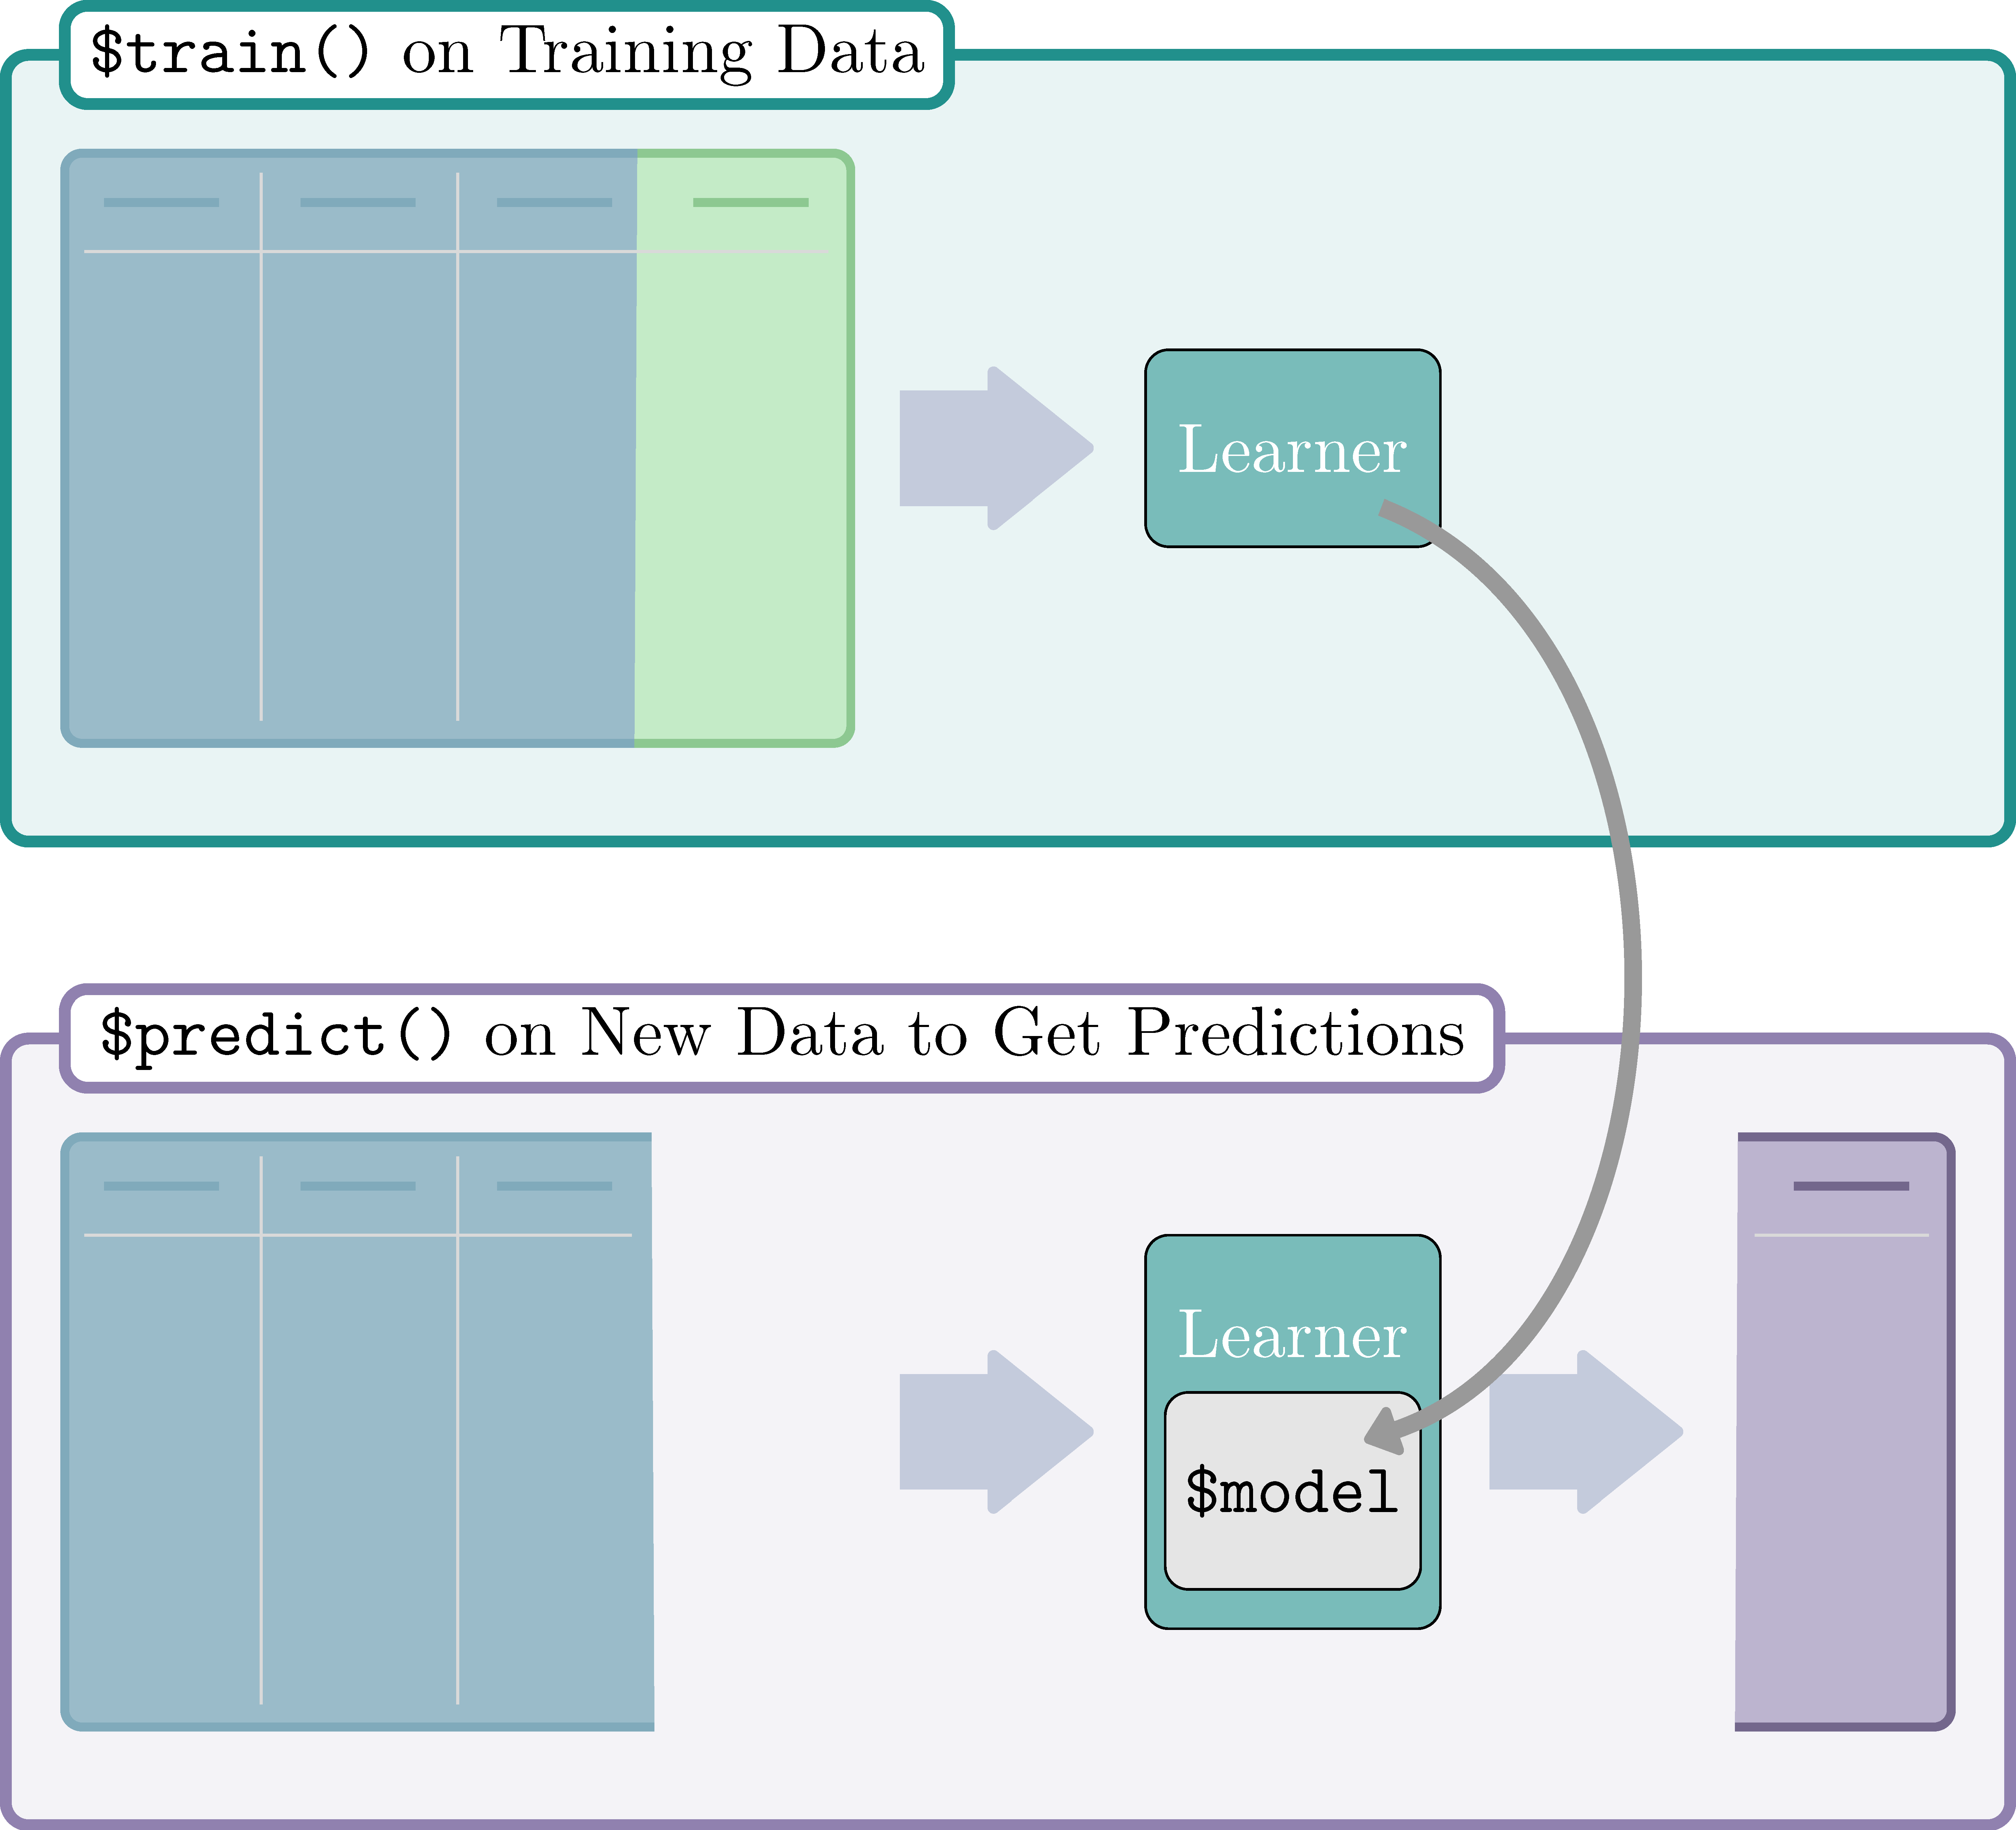
\includegraphics[width=0.7\textwidth,height=\textheight]{chapters/chapter2/Figures/mlr3book_figures-2.png}

}

\caption{\label{fig-basics-learner}Overview of the different stages of a
learner. Top -- data (features and a target) are passed to an
(untrained) learner. Bottom -- new data are passed to the trained model
which makes predictions for the `missing' target column.}

\end{figure}

\hypertarget{sec-training}{%
\subsection{Training}\label{sec-training}}

In the simplest use case, models are trained by passing a task to a
learner with the
\texttt{\$train()}\index{\texttt{Learner}!\texttt{\$train()}}{\marginnote{\begin{footnotesize}\$train()\end{footnotesize}}}
method:

\begin{Shaded}
\begin{Highlighting}[]
\CommentTok{\# load mtcars task}
\NormalTok{tsk\_mtcars }\OtherTok{=} \FunctionTok{tsk}\NormalTok{(}\StringTok{"mtcars"}\NormalTok{)}
\CommentTok{\# load a regression tree}
\NormalTok{lrn\_rpart }\OtherTok{=} \FunctionTok{lrn}\NormalTok{(}\StringTok{"regr.rpart"}\NormalTok{)}
\CommentTok{\# pass the task to the learner via $train()}
\NormalTok{lrn\_rpart}\SpecialCharTok{$}\FunctionTok{train}\NormalTok{(tsk\_mtcars)}
\end{Highlighting}
\end{Shaded}

After training, the fitted model is stored in the
\texttt{\$model}\index{\texttt{Learner}!\texttt{\$model}}{\marginnote{\begin{footnotesize}\$model\end{footnotesize}}}
field for future inspection and prediction:

\begin{Shaded}
\begin{Highlighting}[]
\CommentTok{\# inspect the trained model}
\NormalTok{lrn\_rpart}\SpecialCharTok{$}\NormalTok{model}
\end{Highlighting}
\end{Shaded}

\begin{verbatim}
n= 32 

node), split, n, deviance, yval
      * denotes terminal node

1) root 32 1126.00 20.09  
  2) cyl>=5 21  198.50 16.65  
    4) hp>=192.5 7   28.83 13.41 *
    5) hp< 192.5 14   59.87 18.26 *
  3) cyl< 5 11  203.40 26.66 *
\end{verbatim}

We see that the regression tree has identified features in the task that
are predictive of the target (\texttt{mpg}) and used them to partition
observations. The textual representation of the model depends on the
type of learner. For more information on any model see the learner help
page, which can be accessed in the same way as tasks with the
\texttt{help()} field, e.g., \texttt{lrn\_rpart\$help()}.

\hypertarget{sec-basics-partition}{%
\subsubsection{Partitioning Data}\label{sec-basics-partition}}

When assessing the quality of a model's predictions, you will likely
want to partition your dataset to get a fair and unbiased estimate of a
model's generalization error. In Chapter~\ref{sec-performance} we will
look at resampling and benchmark experiments, which will go into more
detail about performance estimation but for now, we will just discuss
the simplest method of splitting data using the
\href{https://mlr3.mlr-org.com/reference/partition.html}{\texttt{partition()}}\index{\texttt{partition()}}{\marginnote{\begin{footnotesize}\texttt{partition()}\end{footnotesize}}}
function. This function creates index sets that randomly split the given
task into two disjoint sets: a training set\index{training data} (67\%
of the total data by default) and a test set\index{test data} (the
remaining 33\% of the total data not in the training set).

\begin{Shaded}
\begin{Highlighting}[]
\NormalTok{splits }\OtherTok{=} \FunctionTok{partition}\NormalTok{(tsk\_mtcars)}
\NormalTok{splits}
\end{Highlighting}
\end{Shaded}

\begin{verbatim}
$train
 [1]  1  3  4  5  8 10 21 25 32  6  7 11 14 15 16 17 22 31 19 20 26

$test
 [1]  2  9 27 30 12 13 23 24 29 18 28
\end{verbatim}

When training we will tell the model to only use the training data by
passing the row IDs from \texttt{partition} to the \texttt{row\_ids}
argument of \texttt{\$train()}:

\begin{Shaded}
\begin{Highlighting}[]
\NormalTok{lrn\_rpart}\SpecialCharTok{$}\FunctionTok{train}\NormalTok{(tsk\_mtcars, }\AttributeTok{row\_ids =}\NormalTok{ splits}\SpecialCharTok{$}\NormalTok{train)}
\end{Highlighting}
\end{Shaded}

Now we can use our trained learner to make predictions on new data.

\hypertarget{sec-predicting}{%
\subsection{Predicting}\label{sec-predicting}}

Predicting from trained models is as simple as passing your data as a
\texttt{Task} to the
\texttt{\$predict()}\index{\texttt{Learner}!\texttt{\$predict()}}{\marginnote{\begin{footnotesize}\$predict()\end{footnotesize}}}
method of the trained \texttt{Learner}.

Carrying straight on from our last example, we will call the
\texttt{\$predict()} method of our trained learner and again will use
the \texttt{row\_ids} argument, but this time to pass the IDs of our
test set\index{test data}:

\begin{Shaded}
\begin{Highlighting}[]
\NormalTok{prediction }\OtherTok{=}\NormalTok{ lrn\_rpart}\SpecialCharTok{$}\FunctionTok{predict}\NormalTok{(tsk\_mtcars, }\AttributeTok{row\_ids =}\NormalTok{ splits}\SpecialCharTok{$}\NormalTok{test)}
\end{Highlighting}
\end{Shaded}

The \texttt{\$predict()} method returns an object inheriting from
\href{https://mlr3.mlr-org.com/reference/Prediction.html}{\texttt{Prediction}}\index{\texttt{Prediction}}{\marginnote{\begin{footnotesize}\texttt{Prediction}\end{footnotesize}}},
in this case
\href{https://mlr3.mlr-org.com/reference/PredictionRegr.html}{\texttt{PredictionRegr}}\index{\texttt{PredictionRegr}}{\marginnote{\begin{footnotesize}\texttt{PredictionRegr}\end{footnotesize}}}
as this is a regression task.

\begin{Shaded}
\begin{Highlighting}[]
\NormalTok{prediction}
\end{Highlighting}
\end{Shaded}

\begin{verbatim}
<PredictionRegr> for 11 observations:
    row_ids truth response
          2  21.0     24.9
          9  22.8     24.9
         27  26.0     24.9
---                       
         29  15.8     24.9
         18  32.4     24.9
         28  30.4     24.9
\end{verbatim}

The \texttt{row\_ids} column corresponds to the row IDs of the predicted
observations. The \texttt{truth} column contains the ground truth data
if available, which the object extracts from the task, in this case:
\texttt{tsk\_mtcars\$truth(splits\$test)}. Finally, the
\texttt{response} column contains the values predicted by the model. The
\texttt{Prediction} object can easily be converted into a
\texttt{data.table} or \texttt{data.frame} using
\texttt{as.data.table()}/\texttt{as.data.frame()} respectively.

All data in the above columns can be accessed directly, for example, to
get the first two predicted responses:

\begin{Shaded}
\begin{Highlighting}[]
\NormalTok{prediction}\SpecialCharTok{$}\NormalTok{response[}\DecValTok{1}\SpecialCharTok{:}\DecValTok{2}\NormalTok{]}
\end{Highlighting}
\end{Shaded}

\begin{verbatim}
[1] 24.9 24.9
\end{verbatim}

Similarly to plotting \texttt{Task}s,
\href{https://mlr3viz.mlr-org.com}{\texttt{mlr3viz}}\index{\texttt{mlr3viz}}
provides an
\href{https://www.rdocumentation.org/packages/ggplot2/topics/autoplot}{\texttt{autoplot()}}
method for \texttt{Prediction} objects.

\begin{Shaded}
\begin{Highlighting}[]
\FunctionTok{library}\NormalTok{(mlr3viz)}
\NormalTok{prediction }\OtherTok{=}\NormalTok{ lrn\_rpart}\SpecialCharTok{$}\FunctionTok{predict}\NormalTok{(tsk\_mtcars, splits}\SpecialCharTok{$}\NormalTok{test)}
\FunctionTok{autoplot}\NormalTok{(prediction)}
\end{Highlighting}
\end{Shaded}

\begin{figure}[H]

{\centering 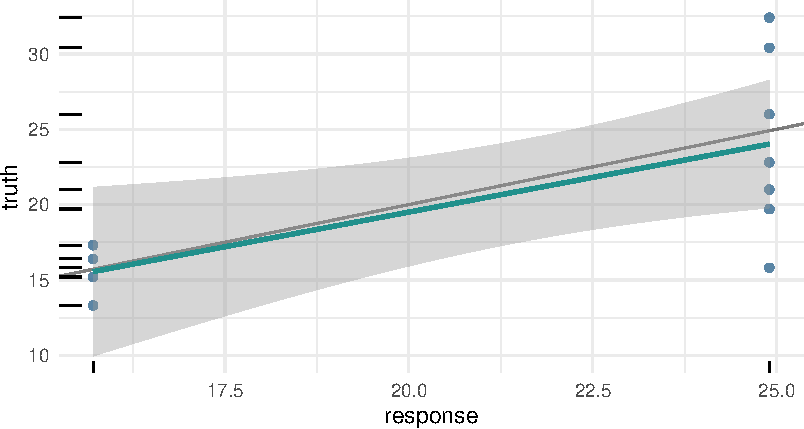
\includegraphics[width=0.7\textwidth,height=\textheight]{chapters/chapter2/data_and_basic_modeling_files/figure-pdf/fig-basics-truthresponse-1.pdf}

}

\caption{\label{fig-basics-truthresponse}Comparing predicted and ground
truth values for the mtcars dataset.}

\end{figure}

In the examples above we made predictions by passing a task to
\texttt{\$predict()}. However, if you would rather pass a
\texttt{data.frame} type object directly, then you can use
\texttt{\$predict\_newdata()}\index{\texttt{Learner}!\texttt{\$predict\_newdata()}}.
Note, the \texttt{truth} column values are all \texttt{NA}, as we did
not include a target column in the generated data.

\begin{Shaded}
\begin{Highlighting}[]
\NormalTok{mtcars\_new }\OtherTok{=} \FunctionTok{data.table}\NormalTok{(}\AttributeTok{cyl =} \FunctionTok{c}\NormalTok{(}\DecValTok{5}\NormalTok{, }\DecValTok{6}\NormalTok{), }\AttributeTok{disp =} \FunctionTok{c}\NormalTok{(}\DecValTok{100}\NormalTok{, }\DecValTok{120}\NormalTok{),}
  \AttributeTok{hp =} \FunctionTok{c}\NormalTok{(}\DecValTok{100}\NormalTok{, }\DecValTok{150}\NormalTok{), }\AttributeTok{drat =} \FunctionTok{c}\NormalTok{(}\DecValTok{4}\NormalTok{, }\FloatTok{3.9}\NormalTok{), }\AttributeTok{wt =} \FunctionTok{c}\NormalTok{(}\FloatTok{3.8}\NormalTok{, }\FloatTok{4.1}\NormalTok{),}
  \AttributeTok{qsec =} \FunctionTok{c}\NormalTok{(}\DecValTok{18}\NormalTok{, }\FloatTok{19.5}\NormalTok{), }\AttributeTok{vs =} \FunctionTok{c}\NormalTok{(}\DecValTok{1}\NormalTok{, }\DecValTok{0}\NormalTok{), }\AttributeTok{am =} \FunctionTok{c}\NormalTok{(}\DecValTok{1}\NormalTok{, }\DecValTok{1}\NormalTok{),}
  \AttributeTok{gear =} \FunctionTok{c}\NormalTok{(}\DecValTok{6}\NormalTok{, }\DecValTok{4}\NormalTok{), }\AttributeTok{carb =} \FunctionTok{c}\NormalTok{(}\DecValTok{3}\NormalTok{, }\DecValTok{5}\NormalTok{))}
\NormalTok{prediction }\OtherTok{=}\NormalTok{ lrn\_rpart}\SpecialCharTok{$}\FunctionTok{predict\_newdata}\NormalTok{(mtcars\_new)}
\NormalTok{prediction}
\end{Highlighting}
\end{Shaded}

\begin{verbatim}
<PredictionRegr> for 2 observations:
 row_ids truth response
       1    NA    15.71
       2    NA    15.71
\end{verbatim}

\hypertarget{changing-the-prediction-type}{%
\subsubsection*{Changing the Prediction
Type}\label{changing-the-prediction-type}}

While predicting a single numeric quantity is the most common prediction
type in regression, it is not the only prediction type. Several
regression models can also predict standard errors. To predict this, the
\texttt{\$predict\_type}\index{\texttt{Learner}!\texttt{\$predict\_type}}
field of a
\href{https://mlr3.mlr-org.com/reference/LearnerRegr.html}{\texttt{LearnerRegr}}
must be changed from ``response'' (the default) to \texttt{"se"} before
training. The \texttt{"rpart"} learner we used above does not support
predicting standard errors, so in the example below we will use a linear
regression model (\texttt{lrn("regr.lm")}).

\begin{Shaded}
\begin{Highlighting}[]
\FunctionTok{library}\NormalTok{(mlr3learners)}
\NormalTok{lrn\_lm }\OtherTok{=} \FunctionTok{lrn}\NormalTok{(}\StringTok{"regr.lm"}\NormalTok{, }\AttributeTok{predict\_type =} \StringTok{"se"}\NormalTok{)}
\NormalTok{lrn\_lm}\SpecialCharTok{$}\FunctionTok{train}\NormalTok{(tsk\_mtcars, splits}\SpecialCharTok{$}\NormalTok{train)}
\NormalTok{lrn\_lm}\SpecialCharTok{$}\FunctionTok{predict}\NormalTok{(tsk\_mtcars, splits}\SpecialCharTok{$}\NormalTok{test)}
\end{Highlighting}
\end{Shaded}

\begin{verbatim}
<PredictionRegr> for 11 observations:
    row_ids truth response    se
          2  21.0    20.20 1.817
          9  22.8    33.32 4.246
         27  26.0    32.22 4.121
---                             
         29  15.8    28.26 4.182
         18  32.4    27.77 1.114
         28  30.4    27.57 2.735
\end{verbatim}

Now the output includes an \texttt{se} column as desired. In
Section~\ref{sec-basics-classif-learner} we will see prediction types
playing an even bigger role in the context of classification.

Having covered the unified train/predict interface, we can now look at
how to use hyperparameters to configure these methods for individual
algorithms.

\hypertarget{sec-param-set}{%
\subsection{Hyperparameters}\label{sec-param-set}}

\texttt{Learner}s encapsulate a machine learning algorithm and its
hyperparameters\index{hyperparameters}, which affect \emph{how} the
algorithm is run and can be set by the user. Hyperparameters may affect
how a model is trained or how it makes predictions and deciding how to
set hyperparameters can require expert knowledge. Hyperparameters can be
optimized automatically (Chapter~\ref{sec-optimization}), but in this
chapter we will focus on how to set them manually.

\hypertarget{paradox-and-parameter-sets}{%
\subsubsection{Paradox and Parameter
Sets}\label{paradox-and-parameter-sets}}

We will continue our running example with a regression tree learner. To
access the hyperparameters in the decision tree, we use
\texttt{\$param\_set}\index{\texttt{Learner}!\texttt{\$param\_set}}{\marginnote{\begin{footnotesize}\$param\_set\end{footnotesize}}}:

\begin{Shaded}
\begin{Highlighting}[]
\NormalTok{lrn\_rpart}\SpecialCharTok{$}\NormalTok{param\_set}
\end{Highlighting}
\end{Shaded}

\begin{verbatim}
<ParamSet>
                id    class lower upper nlevels        default value
 1:             cp ParamDbl     0     1     Inf           0.01      
 2:     keep_model ParamLgl    NA    NA       2          FALSE      
 3:     maxcompete ParamInt     0   Inf     Inf              4      
 4:       maxdepth ParamInt     1    30      30             30      
 5:   maxsurrogate ParamInt     0   Inf     Inf              5      
 6:      minbucket ParamInt     1   Inf     Inf <NoDefault[3]>      
 7:       minsplit ParamInt     1   Inf     Inf             20      
 8: surrogatestyle ParamInt     0     1       2              0      
 9:   usesurrogate ParamInt     0     2       3              2      
10:           xval ParamInt     0   Inf     Inf             10     0
\end{verbatim}

The output above is a
\href{https://paradox.mlr-org.com/reference/ParamSet.html}{\texttt{ParamSet}}\index{\texttt{ParamSet}}{\marginnote{\begin{footnotesize}\texttt{ParamSet}\end{footnotesize}}}
object, supplied by the
\href{https://paradox.mlr-org.com}{\texttt{paradox}} package. These
objects provide information on hyperparameters including their name
(\texttt{id}), data type (\texttt{class}), technically valid ranges for
hyperparameter values (\texttt{lower}, \texttt{upper}), the number of
levels possible if the data type is categorical (\texttt{nlevels}), the
default value from the underlying package (\texttt{default}), and
finally the set value (\texttt{value}). The second column references
classes defined in \href{https://paradox.mlr-org.com}{\texttt{paradox}}
that determine the class of the parameter and the possible values it can
take. Table~\ref{tbl-parameters-classes} lists the possible
hyperparameter types, all of which inherit from
\href{https://paradox.mlr-org.com/reference/Param.html}{\texttt{Param}}.

\hypertarget{tbl-parameters-classes}{}
\begin{longtable}[]{@{}
  >{\raggedright\arraybackslash}p{(\columnwidth - 2\tabcolsep) * \real{0.3333}}
  >{\raggedright\arraybackslash}p{(\columnwidth - 2\tabcolsep) * \real{0.6667}}@{}}
\caption{\label{tbl-parameters-classes}Hyperparameter classes and the
type of hyperparameter they represent.}\tabularnewline
\toprule\noalign{}
\begin{minipage}[b]{\linewidth}\raggedright
Hyperparameter Class
\end{minipage} & \begin{minipage}[b]{\linewidth}\raggedright
Hyperparameter Type
\end{minipage} \\
\midrule\noalign{}
\endfirsthead
\toprule\noalign{}
\begin{minipage}[b]{\linewidth}\raggedright
Hyperparameter Class
\end{minipage} & \begin{minipage}[b]{\linewidth}\raggedright
Hyperparameter Type
\end{minipage} \\
\midrule\noalign{}
\endhead
\bottomrule\noalign{}
\endlastfoot
\href{https://paradox.mlr-org.com/reference/ParamDbl.html}{\texttt{ParamDbl}}\index{\texttt{ParamDbl}}
& Real-valued (numeric) \\
\href{https://paradox.mlr-org.com/reference/ParamInt.html}{\texttt{ParamInt}}\index{\texttt{ParamInt}}
& Integer \\
\href{https://paradox.mlr-org.com/reference/ParamFct.html}{\texttt{ParamFct}}\index{\texttt{ParamFct}}
& Categorical (factor) \\
\href{https://paradox.mlr-org.com/reference/ParamLgl.html}{\texttt{ParamLgl}}\index{\texttt{ParamLgl}}
& Logical / Boolean \\
\href{https://paradox.mlr-org.com/reference/ParamUty.html}{\texttt{ParamUty}}\index{\texttt{ParamUty}}
& Untyped \\
\end{longtable}

In our decision tree example, we can infer from the \texttt{ParamSet}
output that:

\begin{itemize}
\tightlist
\item
  \texttt{cp} must be a ``double'' (\texttt{ParamDbl}) taking values
  between \texttt{0} (\texttt{lower}) and \texttt{1} (\texttt{upper})
  with a default of 0.01 (\texttt{default}).
\item
  \texttt{keep\_model} must be a ``logical'' (\texttt{ParamLgl}) taking
  values \texttt{TRUE} or \texttt{FALSE} with default \texttt{FALSE}
\item
  \texttt{xval} must be an ``integer'' (\texttt{ParamInt}) taking values
  between \texttt{0} and \texttt{Inf} with a default of \texttt{10} and
  has a set value of \texttt{0}.
\end{itemize}

In rare cases (we try to minimize it as much as possible),
hyperparameters are initialized to values which deviate from the default
in the underlying package. When this happens, the reason will always be
given in the learner help page. In the case of
\texttt{lrn("regr.rpart")}, the \texttt{xval} hyperparameter is
initialized to \texttt{0} because \texttt{xval} controls internal
cross-validations and if a user accidentally leaves this at the default
\texttt{10}, model training can take an unnecessarily long time.

\hypertarget{getting-and-setting-hyperparameter-values}{%
\subsubsection{Getting and Setting Hyperparameter
Values}\label{getting-and-setting-hyperparameter-values}}

Now we have looked at how hyperparameter sets are stored, we can think
about getting and setting them. Returning to our decision tree, say we
are interested in growing a tree with depth \texttt{1}, also known as a
``decision stump'', where data is split only once into two terminal
nodes. From the parameter set output, we know that the \texttt{maxdepth}
parameter has a default of \texttt{30} and that it takes integer values.

There are a few different ways we could change this hyperparameter. The
simplest way is during construction of the learner by passing the
hyperparameter name and new value to \texttt{lrn()}:

\begin{Shaded}
\begin{Highlighting}[]
\NormalTok{lrn\_rpart }\OtherTok{=} \FunctionTok{lrn}\NormalTok{(}\StringTok{"regr.rpart"}\NormalTok{, }\AttributeTok{maxdepth =} \DecValTok{1}\NormalTok{)}
\end{Highlighting}
\end{Shaded}

We can get a list of non-default hyperparameters (i.e., those that have
been set) by using \texttt{\$param\_set\$values}:

\begin{Shaded}
\begin{Highlighting}[]
\NormalTok{lrn\_rpart}\SpecialCharTok{$}\NormalTok{param\_set}\SpecialCharTok{$}\NormalTok{values}
\end{Highlighting}
\end{Shaded}

\begin{verbatim}
$xval
[1] 0

$maxdepth
[1] 1
\end{verbatim}

Now we can see that \texttt{maxdepth\ =\ 1} (as we discussed above
\texttt{xval\ =\ 0} is changed during construction) and the learned
regression tree reflects this:

\begin{Shaded}
\begin{Highlighting}[]
\NormalTok{lrn\_rpart}\SpecialCharTok{$}\FunctionTok{train}\NormalTok{(}\FunctionTok{tsk}\NormalTok{(}\StringTok{"mtcars"}\NormalTok{))}\SpecialCharTok{$}\NormalTok{model}
\end{Highlighting}
\end{Shaded}

\begin{verbatim}
n= 32 

node), split, n, deviance, yval
      * denotes terminal node

1) root 32 1126.0 20.09  
  2) cyl>=5 21  198.5 16.65 *
  3) cyl< 5 11  203.4 26.66 *
\end{verbatim}

The \texttt{\$values} field simply returns a \texttt{list} of set
hyperparameters, so another way to update hyperparameters is by updating
an element in the list:

\begin{Shaded}
\begin{Highlighting}[]
\NormalTok{lrn\_rpart}\SpecialCharTok{$}\NormalTok{param\_set}\SpecialCharTok{$}\NormalTok{values}\SpecialCharTok{$}\NormalTok{maxdepth }\OtherTok{=} \DecValTok{2}
\NormalTok{lrn\_rpart}\SpecialCharTok{$}\NormalTok{param\_set}\SpecialCharTok{$}\NormalTok{values}
\end{Highlighting}
\end{Shaded}

\begin{verbatim}
$xval
[1] 0

$maxdepth
[1] 2
\end{verbatim}

\begin{Shaded}
\begin{Highlighting}[]
\CommentTok{\# now with depth 2}
\NormalTok{lrn\_rpart}\SpecialCharTok{$}\FunctionTok{train}\NormalTok{(}\FunctionTok{tsk}\NormalTok{(}\StringTok{"mtcars"}\NormalTok{))}\SpecialCharTok{$}\NormalTok{model}
\end{Highlighting}
\end{Shaded}

\begin{verbatim}
n= 32 

node), split, n, deviance, yval
      * denotes terminal node

1) root 32 1126.00 20.09  
  2) cyl>=5 21  198.50 16.65  
    4) hp>=192.5 7   28.83 13.41 *
    5) hp< 192.5 14   59.87 18.26 *
  3) cyl< 5 11  203.40 26.66 *
\end{verbatim}

To set multiple values at once we recommend either setting these during
construction or using
\texttt{\$set\_values()}\index{\texttt{Learner}!\texttt{\$set\_values()}}{\marginnote{\begin{footnotesize}\$set\_values()\end{footnotesize}}},
which updates the given hyperparameters (argument names) with the
respective values.

\begin{Shaded}
\begin{Highlighting}[]
\NormalTok{lrn\_rpart }\OtherTok{=} \FunctionTok{lrn}\NormalTok{(}\StringTok{"regr.rpart"}\NormalTok{, }\AttributeTok{maxdepth =} \DecValTok{3}\NormalTok{, }\AttributeTok{xval =} \DecValTok{1}\NormalTok{)}
\NormalTok{lrn\_rpart}\SpecialCharTok{$}\NormalTok{param\_set}\SpecialCharTok{$}\NormalTok{values}
\end{Highlighting}
\end{Shaded}

\begin{verbatim}
$xval
[1] 1

$maxdepth
[1] 3
\end{verbatim}

\begin{Shaded}
\begin{Highlighting}[]
\CommentTok{\# or with set\_values}
\NormalTok{lrn\_rpart}\SpecialCharTok{$}\NormalTok{param\_set}\SpecialCharTok{$}\FunctionTok{set\_values}\NormalTok{(}\AttributeTok{xval =} \DecValTok{2}\NormalTok{, }\AttributeTok{cp =} \FloatTok{0.5}\NormalTok{)}
\NormalTok{lrn\_rpart}\SpecialCharTok{$}\NormalTok{param\_set}\SpecialCharTok{$}\NormalTok{values}
\end{Highlighting}
\end{Shaded}

\begin{verbatim}
$xval
[1] 2

$maxdepth
[1] 3

$cp
[1] 0.5
\end{verbatim}

\begin{tcolorbox}[enhanced jigsaw, opacitybacktitle=0.6, rightrule=.15mm, opacityback=0, arc=.35mm, breakable, titlerule=0mm, colframe=quarto-callout-warning-color-frame, coltitle=black, bottomrule=.15mm, toprule=.15mm, colback=white, colbacktitle=quarto-callout-warning-color!10!white, bottomtitle=1mm, toptitle=1mm, title=\textcolor{quarto-callout-warning-color}{\faExclamationTriangle}\hspace{0.5em}{Setting Hyperparameters Using a \texttt{list}}, leftrule=.75mm, left=2mm]

As \texttt{lrn\_rpart\$param\_set\$values} returns a \texttt{list}, some
users may be tempted to set hyperparameters by passing a new
\texttt{list} to \texttt{\$values} -- this would work but \textbf{we do
not recommend it}. This is because passing a \texttt{list} will wipe any
existing hyperparameter values if they are not included in the list. For
example:

\begin{Shaded}
\begin{Highlighting}[]
\CommentTok{\# set xval and cp}
\NormalTok{lrn\_rpart\_params }\OtherTok{=} \FunctionTok{lrn}\NormalTok{(}\StringTok{"regr.rpart"}\NormalTok{, }\AttributeTok{xval =} \DecValTok{0}\NormalTok{, }\AttributeTok{cp =} \DecValTok{1}\NormalTok{)}
\CommentTok{\# passing maxdepth through a list, removing all other values}
\NormalTok{lrn\_rpart\_params}\SpecialCharTok{$}\NormalTok{param\_set}\SpecialCharTok{$}\NormalTok{values }\OtherTok{=} \FunctionTok{list}\NormalTok{(}\AttributeTok{maxdepth =} \DecValTok{1}\NormalTok{)}
\CommentTok{\# we have removed xval and cp by mistake}
\NormalTok{lrn\_rpart\_params}\SpecialCharTok{$}\NormalTok{param\_set}\SpecialCharTok{$}\NormalTok{values}
\end{Highlighting}
\end{Shaded}

\begin{verbatim}
$maxdepth
[1] 1
\end{verbatim}

\begin{Shaded}
\begin{Highlighting}[]
\CommentTok{\# now with set\_values}
\NormalTok{lrn\_rpart\_params }\OtherTok{=} \FunctionTok{lrn}\NormalTok{(}\StringTok{"regr.rpart"}\NormalTok{, }\AttributeTok{xval =} \DecValTok{0}\NormalTok{, }\AttributeTok{cp =} \DecValTok{1}\NormalTok{)}
\NormalTok{lrn\_rpart\_params}\SpecialCharTok{$}\NormalTok{param\_set}\SpecialCharTok{$}\FunctionTok{set\_values}\NormalTok{(}\AttributeTok{maxdepth =} \DecValTok{1}\NormalTok{)}
\NormalTok{lrn\_rpart\_params}\SpecialCharTok{$}\NormalTok{param\_set}\SpecialCharTok{$}\NormalTok{values}
\end{Highlighting}
\end{Shaded}

\begin{verbatim}
$xval
[1] 0

$cp
[1] 1

$maxdepth
[1] 1
\end{verbatim}

\end{tcolorbox}

Whichever method you choose, all have safety checks to ensure your new
values fall within the allowed parameter range:

\begin{Shaded}
\begin{Highlighting}[]
\FunctionTok{lrn}\NormalTok{(}\StringTok{"regr.rpart"}\NormalTok{, }\AttributeTok{cp =} \DecValTok{2}\NormalTok{, }\AttributeTok{maxdepth =} \DecValTok{2}\NormalTok{)}
\end{Highlighting}
\end{Shaded}

\begin{verbatim}
Error in self$assert(xs): Assertion on 'xs' failed: cp:
	Element 1 is not <= 1.
\end{verbatim}

\hypertarget{hyperparameter-dependencies}{%
\subsubsection{Hyperparameter
Dependencies}\label{hyperparameter-dependencies}}

\begin{tcolorbox}[enhanced jigsaw, colframe=quarto-callout-note-color-frame, rightrule=.15mm, bottomrule=.15mm, toprule=.15mm, opacityback=0, colback=white, left=2mm, arc=.35mm, breakable, leftrule=.75mm]
\begin{minipage}[t]{5.5mm}
\textcolor{quarto-callout-note-color}{\faInfo}
\end{minipage}%
\begin{minipage}[t]{\textwidth - 5.5mm}

\textbf{This section covers advanced ML or technical
details.}\vspace{2mm}

\end{minipage}%
\end{tcolorbox}

More complex hyperparameter spaces may include dependencies, which occur
when setting a hyperparameter is conditional on the value of another
hyperparameter; this is most important in the context of model tuning
(Chapter~\ref{sec-optimization}). One such example is a support vector
machine\index{support vector machine} (\texttt{lrn("regr.svm")}). The
field \texttt{\$deps}\index{\texttt{ParamSet}!\texttt{\$deps}} returns a
\texttt{data.table}, which lists the hyperparameter dependencies in the
\texttt{Learner}. For example we can see that the \texttt{cost}
(\texttt{id}-column) parameter is dependent on the \texttt{type}
(\texttt{on}-column) parameter.

\begin{Shaded}
\begin{Highlighting}[]
\FunctionTok{lrn}\NormalTok{(}\StringTok{"regr.svm"}\NormalTok{)}\SpecialCharTok{$}\NormalTok{param\_set}\SpecialCharTok{$}\NormalTok{deps}
\end{Highlighting}
\end{Shaded}

\begin{verbatim}
        id     on           cond
1:    cost   type <CondAnyOf[9]>
2:      nu   type <CondEqual[9]>
3:  degree kernel <CondEqual[9]>
4:   coef0 kernel <CondAnyOf[9]>
5:   gamma kernel <CondAnyOf[9]>
6: epsilon   type <CondEqual[9]>
\end{verbatim}

The \texttt{cond} column tells us what the condition is, which will
either mean that \texttt{id} can be set if \texttt{on} equals a single
value
(\href{https://paradox.mlr-org.com/reference/Condition.html}{\texttt{CondEqual}})
or any value in the listed set
(\href{https://paradox.mlr-org.com/reference/Condition.html}{\texttt{CondAnyOf}}).

\begin{Shaded}
\begin{Highlighting}[]
\FunctionTok{lrn}\NormalTok{(}\StringTok{"regr.svm"}\NormalTok{)}\SpecialCharTok{$}\NormalTok{param\_set}\SpecialCharTok{$}\NormalTok{deps[[}\DecValTok{1}\NormalTok{, }\StringTok{"cond"}\NormalTok{]]}
\end{Highlighting}
\end{Shaded}

\begin{verbatim}
CondAnyOf: x ∈ {eps-regression, nu-regression}
\end{verbatim}

\begin{Shaded}
\begin{Highlighting}[]
\FunctionTok{lrn}\NormalTok{(}\StringTok{"regr.svm"}\NormalTok{)}\SpecialCharTok{$}\NormalTok{param\_set}\SpecialCharTok{$}\NormalTok{deps[[}\DecValTok{3}\NormalTok{, }\StringTok{"cond"}\NormalTok{]]}
\end{Highlighting}
\end{Shaded}

\begin{verbatim}
CondEqual: x = polynomial
\end{verbatim}

This tells us that the parameter \texttt{cost} should only be set if the
\texttt{type} parameter is one of \texttt{"eps-regression"} or
\texttt{"nu-regression"}, and \texttt{degree} should only be set if
\texttt{kernel} is equal to \texttt{"polynomial"}.

The \texttt{Learner} will error if dependent hyperparameters are set
when their conditions are not met:

\begin{Shaded}
\begin{Highlighting}[]
\CommentTok{\# error as kernel is not polynomial}
\FunctionTok{lrn}\NormalTok{(}\StringTok{"regr.svm"}\NormalTok{, }\AttributeTok{kernel =} \StringTok{"linear"}\NormalTok{, }\AttributeTok{degree =} \DecValTok{1}\NormalTok{)}
\end{Highlighting}
\end{Shaded}

\begin{verbatim}
Error in self$assert(xs): Assertion on 'xs' failed: The parameter 'degree'
	can only be set if the following condition is met 'kernel = polynomial'.
	Instead the current parameter value is: kernel=linear.
\end{verbatim}

\begin{Shaded}
\begin{Highlighting}[]
\CommentTok{\# works because kernel is polynomial}
\FunctionTok{lrn}\NormalTok{(}\StringTok{"regr.svm"}\NormalTok{, }\AttributeTok{kernel =} \StringTok{"polynomial"}\NormalTok{, }\AttributeTok{degree =} \DecValTok{1}\NormalTok{)}
\end{Highlighting}
\end{Shaded}

\begin{verbatim}
<LearnerRegrSVM:regr.svm>
* Model: -
* Parameters: kernel=polynomial, degree=1
* Packages: mlr3, mlr3learners, e1071
* Predict Types:  [response]
* Feature Types: logical, integer, numeric
* Properties: -
\end{verbatim}

\hypertarget{sec-basics-featureless}{%
\subsection{Baseline Learners}\label{sec-basics-featureless}}

Before we move on to learner evaluation, we will highlight an important
class of learners. These are extremely simple or `weak' learners known
as
baselines\index{baselines}{\marginnote{\begin{footnotesize}Baselines\end{footnotesize}}}.
Baselines are useful in model comparison (Chapter~\ref{sec-performance})
and as fallback learners (Section~\ref{sec-encapsulation-fallback},
Section~\ref{sec-fallback}). For regression, we have implemented the
baseline \texttt{lrn("regr.featureless")}, which always predicts new
values to be the mean (or median, if the \texttt{robust} hyperparameter
is set to \texttt{TRUE}) of the target in the training data:

\begin{Shaded}
\begin{Highlighting}[]
\CommentTok{\# generate data}
\NormalTok{df }\OtherTok{=} \FunctionTok{as\_task\_regr}\NormalTok{(}\FunctionTok{data.frame}\NormalTok{(}\AttributeTok{x =} \FunctionTok{runif}\NormalTok{(}\DecValTok{1000}\NormalTok{), }\AttributeTok{y =} \FunctionTok{rnorm}\NormalTok{(}\DecValTok{1000}\NormalTok{, }\DecValTok{2}\NormalTok{, }\DecValTok{1}\NormalTok{)),}
  \AttributeTok{target =} \StringTok{"y"}\NormalTok{)}
\FunctionTok{lrn}\NormalTok{(}\StringTok{"regr.featureless"}\NormalTok{)}\SpecialCharTok{$}\FunctionTok{train}\NormalTok{(df, }\DecValTok{1}\SpecialCharTok{:}\DecValTok{995}\NormalTok{)}\SpecialCharTok{$}\FunctionTok{predict}\NormalTok{(df, }\DecValTok{996}\SpecialCharTok{:}\DecValTok{1000}\NormalTok{)}
\end{Highlighting}
\end{Shaded}

\begin{verbatim}
<PredictionRegr> for 5 observations:
 row_ids truth response
     996 2.996    1.976
     997 3.675    1.976
     998 3.651    1.976
     999 1.803    1.976
    1000 1.196    1.976
\end{verbatim}

It is good practice to test all new models against a baseline, and also
to include baselines in experiments with multiple other models. In
general, a model that does not outperform a baseline is a `bad' model,
on the other hand, a model is not necessarily `good' if it outperforms
the baseline.

\hypertarget{sec-eval}{%
\section{Evaluation}\label{sec-eval}}

Perhaps \emph{the most} important step of the applied machine learning
workflow is evaluating model performance. Without this, we would have no
way to know if our trained model makes very accurate predictions, is
worse than randomly guessing, or somewhere in between. We will continue
with our decision tree example to establish if the quality of our
predictions is `good', first we will rerun the above code so it is
easier to follow along.

\begin{Shaded}
\begin{Highlighting}[]
\NormalTok{lrn\_rpart }\OtherTok{=} \FunctionTok{lrn}\NormalTok{(}\StringTok{"regr.rpart"}\NormalTok{)}
\NormalTok{tsk\_mtcars }\OtherTok{=} \FunctionTok{tsk}\NormalTok{(}\StringTok{"mtcars"}\NormalTok{)}
\NormalTok{splits }\OtherTok{=} \FunctionTok{partition}\NormalTok{(tsk\_mtcars)}
\NormalTok{lrn\_rpart}\SpecialCharTok{$}\FunctionTok{train}\NormalTok{(tsk\_mtcars, splits}\SpecialCharTok{$}\NormalTok{train)}
\NormalTok{prediction }\OtherTok{=}\NormalTok{ lrn\_rpart}\SpecialCharTok{$}\FunctionTok{predict}\NormalTok{(tsk\_mtcars, splits}\SpecialCharTok{$}\NormalTok{test)}
\end{Highlighting}
\end{Shaded}

\hypertarget{measures}{%
\subsection{Measures}\label{measures}}

The quality of predictions is evaluated using measures that compare them
to the ground truth data for supervised learning tasks. Similarly to
\texttt{Task}s and \texttt{Learner}s, the available measures in
\texttt{mlr3} are stored in a dictionary called
\href{https://mlr3.mlr-org.com/reference/mlr_measures.html}{\texttt{mlr\_measures}}\index{\texttt{mlr\_measures}}
and can be accessed with
\texttt{msr()}\index{\texttt{msr()/msrs()}}{\marginnote{\begin{footnotesize}msr()\end{footnotesize}}}:

\begin{Shaded}
\begin{Highlighting}[]
\FunctionTok{as.data.table}\NormalTok{(}\FunctionTok{msr}\NormalTok{())}
\end{Highlighting}
\end{Shaded}

\begin{verbatim}
             key                          label task_type
 1:          aic   Akaike Information Criterion      <NA>
 2:          bic Bayesian Information Criterion      <NA>
 3:  classif.acc        Classification Accuracy   classif
 4:  classif.auc       Area Under the ROC Curve   classif
 5: classif.bacc              Balanced Accuracy   classif
---                                                      
62:  sim.jaccard       Jaccard Similarity Index      <NA>
63:      sim.phi     Phi Coefficient Similarity      <NA>
64:    time_both                   Elapsed Time      <NA>
65: time_predict                   Elapsed Time      <NA>
66:   time_train                   Elapsed Time      <NA>
3 variables not shown: [packages, predict_type, task_properties]
\end{verbatim}

All measures implemented in \texttt{mlr3} are defined primarily by three
components: 1) the function that defines the measure; 2) whether a lower
or higher value is considered `good'; and 3) the range of possible
values the measure can take. As well as these defining elements, other
metadata are important to consider when selecting and using a
\texttt{Measure}, including if the measure has any special properties
(e.g., requires training data), the type of predictions the measure can
evaluate, and whether the measure has any `control parameters'. All this
information is encapsulated in the
\href{https://mlr3.mlr-org.com/reference/Measure.html}{\texttt{Measure}}\index{\texttt{Measure}}{\marginnote{\begin{footnotesize}\texttt{Measure}\end{footnotesize}}}
object. By example, let us consider the mean absolute
error\index{mean absolute error} (MAE):

\begin{Shaded}
\begin{Highlighting}[]
\NormalTok{measure }\OtherTok{=} \FunctionTok{msr}\NormalTok{(}\StringTok{"regr.mae"}\NormalTok{)}
\NormalTok{measure}
\end{Highlighting}
\end{Shaded}

\begin{verbatim}
<MeasureRegrSimple:regr.mae>: Mean Absolute Error
* Packages: mlr3, mlr3measures
* Range: [0, Inf]
* Minimize: TRUE
* Average: macro
* Parameters: list()
* Properties: -
* Predict type: response
\end{verbatim}

This measure compares the absolute difference (`error') between true and
predicted values: \(f(y, \hat{y}) = | y - \hat{y} |\). Lower values are
considered better (\texttt{Minimize:\ TRUE}), which is intuitive as we
would like the true values, \(y\), to be identical (or as close as
possible) in value to the predicted values, \(\hat{y}\). We can see that
the range of possible values the learner can take is from \(0\) to
\(\infty\) (\texttt{Range:\ {[}0,\ Inf{]}}), it has no special
properties (\texttt{Properties:\ -}), it evaluates \texttt{response}
type predictions for regression models
(\texttt{Predict\ type:\ response}), and it has no control parameters
(\texttt{Parameters:\ list()}).

Now let us see how to use this measure for scoring our predictions.

\hypertarget{scoring-predictions}{%
\subsection{Scoring Predictions}\label{scoring-predictions}}

Usually, supervised learning measures compare the difference between
predicted values and the ground truth. \texttt{mlr3} simplifies the
process of bringing these quantities together by storing the predictions
and true outcomes in the
\href{https://mlr3.mlr-org.com/reference/Prediction.html}{\texttt{Prediction}}\index{\texttt{Prediction}}
object as we have already seen.

\begin{Shaded}
\begin{Highlighting}[]
\NormalTok{prediction}
\end{Highlighting}
\end{Shaded}

\begin{verbatim}
<PredictionRegr> for 11 observations:
    row_ids truth response
          2  21.0    16.70
          8  24.4    26.81
         21  21.5    26.81
---                       
         31  15.0    16.70
         18  32.4    26.81
         26  27.3    26.81
\end{verbatim}

To calculate model performance, we simply call the
\texttt{\$score()}\index{\texttt{Prediction}!\texttt{\$score()}}{\marginnote{\begin{footnotesize}\$score()\end{footnotesize}}}
method of a \texttt{Prediction} object and pass as a single argument the
measure that we want to compute:

\begin{Shaded}
\begin{Highlighting}[]
\NormalTok{prediction}\SpecialCharTok{$}\FunctionTok{score}\NormalTok{(measure)}
\end{Highlighting}
\end{Shaded}

\begin{verbatim}
regr.mae 
   2.591 
\end{verbatim}

Note that all task types have default measures that are used if the
argument to \texttt{\$score()} is omitted, for regression this is the
mean squared error (\texttt{msr("regr.mse")}), which is the squared
difference between true and predicted values:
\(f(y, \hat{y}) = (y - \hat{y})^2\), averaged over the test set.

It is possible to calculate multiple measures at the same time by
passing multiple measures to \texttt{\$score()}. For example, below we
compute performance for mean squared error (\texttt{"regr.mse"}) and
mean absolute error (\texttt{"regr.mae"}) -- note we use
\texttt{msrs()}\index{\texttt{msr()/msrs()}}{\marginnote{\begin{footnotesize}msrs()\end{footnotesize}}}
to load multiple measures at once.

\begin{Shaded}
\begin{Highlighting}[]
\NormalTok{measures }\OtherTok{=} \FunctionTok{msrs}\NormalTok{(}\FunctionTok{c}\NormalTok{(}\StringTok{"regr.mse"}\NormalTok{, }\StringTok{"regr.mae"}\NormalTok{))}
\NormalTok{prediction}\SpecialCharTok{$}\FunctionTok{score}\NormalTok{(measures)}
\end{Highlighting}
\end{Shaded}

\begin{verbatim}
regr.mse regr.mae 
   9.567    2.591 
\end{verbatim}

\hypertarget{sec-basics-measures-tech}{%
\subsection{Technical Measures}\label{sec-basics-measures-tech}}

\begin{tcolorbox}[enhanced jigsaw, colframe=quarto-callout-note-color-frame, rightrule=.15mm, bottomrule=.15mm, toprule=.15mm, opacityback=0, colback=white, left=2mm, arc=.35mm, breakable, leftrule=.75mm]
\begin{minipage}[t]{5.5mm}
\textcolor{quarto-callout-note-color}{\faInfo}
\end{minipage}%
\begin{minipage}[t]{\textwidth - 5.5mm}

\textbf{This section covers advanced ML or technical
details.}\vspace{2mm}

\end{minipage}%
\end{tcolorbox}

\texttt{mlr3} also provides measures that do not quantify the quality of
the predictions of a model, but instead provide `meta'-information about
the model. These include:

\begin{itemize}
\tightlist
\item
  \texttt{msr("time\_train")} -- The time taken to train a model.
\item
  \texttt{msr("time\_predict")} -- The time taken for the model to make
  predictions.
\item
  \texttt{msr("time\_both")} -- The total time taken to train the model
  and then make predictions.
\item
  \texttt{msr("selected\_features")} -- The number of features selected
  by a model, which can only be used if the model has the
  ``selected\_features'' property.
\end{itemize}

For example, we could score our decision tree to see how many seconds it
took to train the model and make predictions:

\begin{Shaded}
\begin{Highlighting}[]
\NormalTok{measures }\OtherTok{=} \FunctionTok{msrs}\NormalTok{(}\FunctionTok{c}\NormalTok{(}\StringTok{"time\_train"}\NormalTok{, }\StringTok{"time\_predict"}\NormalTok{, }\StringTok{"time\_both"}\NormalTok{))}
\NormalTok{prediction}\SpecialCharTok{$}\FunctionTok{score}\NormalTok{(measures, }\AttributeTok{learner =}\NormalTok{ lrn\_rpart)}
\end{Highlighting}
\end{Shaded}

\begin{verbatim}
  time_train time_predict    time_both 
       0.002        0.001        0.003 
\end{verbatim}

Notice a few key properties of these measures:

\begin{enumerate}
\def\labelenumi{\arabic{enumi})}
\tightlist
\item
  \texttt{time\_both} is simply the sum of \texttt{time\_train} and
  \texttt{time\_predict}.
\item
  We had to pass \texttt{learner\ =\ lrn\_rpart} to \texttt{\$score()}
  as these measures have the \texttt{requires\_learner} property:
\end{enumerate}

\begin{Shaded}
\begin{Highlighting}[]
\FunctionTok{msr}\NormalTok{(}\StringTok{"time\_train"}\NormalTok{)}\SpecialCharTok{$}\NormalTok{properties}
\end{Highlighting}
\end{Shaded}

\begin{verbatim}
[1] "requires_learner"
\end{verbatim}

\begin{enumerate}
\def\labelenumi{\arabic{enumi})}
\setcounter{enumi}{2}
\tightlist
\item
  These can be used after model training and predicting because we
  automatically store model run times whenever \texttt{\$train()} and
  \texttt{\$predict()} are called, so the measures above are equivalent
  to:
\end{enumerate}

\begin{Shaded}
\begin{Highlighting}[]
\FunctionTok{c}\NormalTok{(lrn\_rpart}\SpecialCharTok{$}\NormalTok{timings, }\AttributeTok{both =} \FunctionTok{sum}\NormalTok{(lrn\_rpart}\SpecialCharTok{$}\NormalTok{timings))}
\end{Highlighting}
\end{Shaded}

\begin{verbatim}
  train predict    both 
  0.002   0.001   0.003 
\end{verbatim}

The \texttt{selected\_features} measure calculates how many features
were used in the fitted model.

\begin{Shaded}
\begin{Highlighting}[]
\NormalTok{msr\_sf }\OtherTok{=} \FunctionTok{msr}\NormalTok{(}\StringTok{"selected\_features"}\NormalTok{)}
\NormalTok{msr\_sf}
\end{Highlighting}
\end{Shaded}

\begin{verbatim}
<MeasureSelectedFeatures:selected_features>: Absolute or Relative Frequency
	of Selected Features
* Packages: mlr3
* Range: [0, Inf]
* Minimize: TRUE
* Average: macro
* Parameters: normalize=FALSE
* Properties: requires_task, requires_learner, requires_model
* Predict type: NA
\end{verbatim}

We can see that this measure contains control
parameters\index{control parameters}{\marginnote{\begin{footnotesize}Control
Parameters\end{footnotesize}}} (\texttt{Parameters:\ normalize=FALSE}),
which control how the measure is computed. As with hyperparameters these
can be accessed with
\texttt{\$param\_set}\index{\texttt{Measure}!\texttt{\$param\_set}}:

\begin{Shaded}
\begin{Highlighting}[]
\NormalTok{msr\_sf }\OtherTok{=} \FunctionTok{msr}\NormalTok{(}\StringTok{"selected\_features"}\NormalTok{)}
\NormalTok{msr\_sf}\SpecialCharTok{$}\NormalTok{param\_set}
\end{Highlighting}
\end{Shaded}

\begin{verbatim}
<ParamSet>
          id    class lower upper nlevels default value
1: normalize ParamLgl    NA    NA       2   FALSE FALSE
\end{verbatim}

The \texttt{normalize} hyperparameter specifies whether the returned
number of selected features should be normalized by the total number of
features, this is useful if you are comparing this value across tasks
with differing numbers of features. We would change this parameter in
the exact same way as we did with the learner above:

\begin{Shaded}
\begin{Highlighting}[]
\NormalTok{msr\_sf}\SpecialCharTok{$}\NormalTok{param\_set}\SpecialCharTok{$}\NormalTok{values}\SpecialCharTok{$}\NormalTok{normalize }\OtherTok{=} \ConstantTok{TRUE}
\NormalTok{prediction}\SpecialCharTok{$}\FunctionTok{score}\NormalTok{(msr\_sf, }\AttributeTok{task =}\NormalTok{ tsk\_mtcars, }\AttributeTok{learner =}\NormalTok{ lrn\_rpart)}
\end{Highlighting}
\end{Shaded}

\begin{verbatim}
selected_features 
              0.1 
\end{verbatim}

Note that we passed the task and learner as the measure has the
\texttt{requires\_task} and \texttt{requires\_learner} properties.

\hypertarget{sec-basics-regr-experiment}{%
\section{Our First Regression
Experiment}\label{sec-basics-regr-experiment}}

We have now seen how to train a model, make predictions and score them.
What we have not yet attempted is to ascertain if our predictions are
any `good'. So before look at how the building blocks of \texttt{mlr3}
extend to classification, we will take a brief pause to put together
everything above in a short experiment to assess the quality of our
predictions. We will do this by comparing the performance of a
featureless regression learner to a decision tree with changed
hyperparameters.

\begin{Shaded}
\begin{Highlighting}[]
\FunctionTok{library}\NormalTok{(mlr3)}
\FunctionTok{set.seed}\NormalTok{(}\DecValTok{349}\NormalTok{)}
\CommentTok{\# load and partition our task}
\NormalTok{tsk\_mtcars }\OtherTok{=} \FunctionTok{tsk}\NormalTok{(}\StringTok{"mtcars"}\NormalTok{)}
\NormalTok{splits }\OtherTok{=} \FunctionTok{partition}\NormalTok{(tsk\_mtcars)}
\CommentTok{\# load featureless learner}
\NormalTok{lrn\_featureless }\OtherTok{=} \FunctionTok{lrn}\NormalTok{(}\StringTok{"regr.featureless"}\NormalTok{)}
\CommentTok{\# load decision tree and set hyperparameters}
\NormalTok{lrn\_rpart }\OtherTok{=} \FunctionTok{lrn}\NormalTok{(}\StringTok{"regr.rpart"}\NormalTok{, }\AttributeTok{cp =} \FloatTok{0.2}\NormalTok{, }\AttributeTok{maxdepth =} \DecValTok{5}\NormalTok{)}
\CommentTok{\# load MSE and MAE measures}
\NormalTok{measures }\OtherTok{=} \FunctionTok{msrs}\NormalTok{(}\FunctionTok{c}\NormalTok{(}\StringTok{"regr.mse"}\NormalTok{, }\StringTok{"regr.mae"}\NormalTok{))}
\CommentTok{\# train learners}
\NormalTok{lrn\_featureless}\SpecialCharTok{$}\FunctionTok{train}\NormalTok{(tsk\_mtcars, splits}\SpecialCharTok{$}\NormalTok{train)}
\NormalTok{lrn\_rpart}\SpecialCharTok{$}\FunctionTok{train}\NormalTok{(tsk\_mtcars, splits}\SpecialCharTok{$}\NormalTok{train)}
\CommentTok{\# make and score predictions}
\NormalTok{lrn\_featureless}\SpecialCharTok{$}\FunctionTok{predict}\NormalTok{(tsk\_mtcars, splits}\SpecialCharTok{$}\NormalTok{test)}\SpecialCharTok{$}\FunctionTok{score}\NormalTok{(measures)}
\end{Highlighting}
\end{Shaded}

\begin{verbatim}
regr.mse regr.mae 
  26.727    4.513 
\end{verbatim}

\begin{Shaded}
\begin{Highlighting}[]
\NormalTok{lrn\_rpart}\SpecialCharTok{$}\FunctionTok{predict}\NormalTok{(tsk\_mtcars, splits}\SpecialCharTok{$}\NormalTok{test)}\SpecialCharTok{$}\FunctionTok{score}\NormalTok{(measures)}
\end{Highlighting}
\end{Shaded}

\begin{verbatim}
regr.mse regr.mae 
   6.933    2.206 
\end{verbatim}

Before starting the experiment we load the \texttt{mlr3} library and set
a seed. We loaded the \texttt{mtcars} task using \texttt{tsk()} and then
split this using \texttt{partition} with the default 2/3 split. Next, we
loaded a featureless baseline learner (\texttt{"regr.featureless"}) with
the \texttt{lrn()} function. Then loaded a decision tree
(\texttt{lrn("regr.rpart")}) but changed the complexity parameter and
max tree depth from their defaults. We then used \texttt{msrs()} to load
multiple measures at once, the mean squared error (MSE:
\texttt{regr.mse}) and the mean absolute error (MAE: \texttt{regr.mae}).
With all objects loaded, we trained our models, ensuring we passed the
same training data to both. Finally, we made predictions from our
trained models and scored these. For both MSE and MAE, lower values are
`better' (\texttt{Minimize:\ TRUE}) and we can therefore conclude that
our decision tree performs better than the featureless baseline. In
Section~\ref{sec-benchmarking} we will see how to formalize comparison
between models in a more efficient way using
\href{https://mlr3.mlr-org.com/reference/benchmark.html}{\texttt{benchmark()}}\index{\texttt{benchmark()}}.

Now we have put everything together you may notice that our learners and
measures both have the \texttt{"regr."} prefix, which is a handy way of
reminding us that we are working with a regression task and therefore
must make use of learners and measures built for regression. In the next
section, we will extend the building blocks of \texttt{mlr3} to consider
classification tasks, which make use of learners and measures with the
\texttt{"classif."} prefix.

\hypertarget{sec-classif}{%
\section{Classification}\label{sec-classif}}

Classification\index{classification} problems are ones in which a model
predicts a discrete, categorical target, as opposed to a continuous,
numeric quantity. For example, predicting the species of penguin from
its physical characteristics would be a classification problem as there
is a defined set of species. \texttt{mlr3} ensures that the interface
for all tasks is as similar as possible (if not identical) and therefore
we will not repeat any content from the previous section but will just
focus on differences that make classification a unique machine learning
problem. We will first demonstrate the similarities between regression
and classification by performing an experiment very similar to the one
in Section~\ref{sec-basics-regr-experiment}, using code that will now be
familiar to you. We will then move to differences in tasks, learners and
predictions, before looking at thresholding\index{thresholding}, which
is a method specific to classification.

\hypertarget{sec-basics-classif-experiment}{%
\subsection{Our First Classification
Experiment}\label{sec-basics-classif-experiment}}

The interface for classification tasks, learners, and measures, is
identical to the regression setting, except the underlying objects
inherit from
\href{https://mlr3.mlr-org.com/reference/TaskClassif.html}{\texttt{TaskClassif}}\index{\texttt{TaskClassif}},
\href{https://mlr3.mlr-org.com/reference/LearnerClassif.html}{\texttt{LearnerClassif}}\index{\texttt{LearnerClassif}},
and
\href{https://mlr3.mlr-org.com/reference/MeasureClassif.html}{\texttt{MeasureClassif}}\index{\texttt{MeasureClassif}},
respectively. We can therefore run a very similar experiment to the one
above.

\begin{Shaded}
\begin{Highlighting}[]
\FunctionTok{library}\NormalTok{(mlr3)}
\FunctionTok{set.seed}\NormalTok{(}\DecValTok{349}\NormalTok{)}
\CommentTok{\# load and partition our task}
\NormalTok{tsk\_penguins }\OtherTok{=} \FunctionTok{tsk}\NormalTok{(}\StringTok{"penguins"}\NormalTok{)}
\NormalTok{splits }\OtherTok{=} \FunctionTok{partition}\NormalTok{(tsk\_penguins)}
\CommentTok{\# load featureless learner}
\NormalTok{lrn\_featureless }\OtherTok{=} \FunctionTok{lrn}\NormalTok{(}\StringTok{"classif.featureless"}\NormalTok{)}
\CommentTok{\# load decision tree and set hyperparameters}
\NormalTok{lrn\_rpart }\OtherTok{=} \FunctionTok{lrn}\NormalTok{(}\StringTok{"classif.rpart"}\NormalTok{, }\AttributeTok{cp =} \FloatTok{0.2}\NormalTok{, }\AttributeTok{maxdepth =} \DecValTok{5}\NormalTok{)}
\CommentTok{\# load accuracy measure}
\NormalTok{measure }\OtherTok{=} \FunctionTok{msr}\NormalTok{(}\StringTok{"classif.acc"}\NormalTok{)}
\CommentTok{\# train learners}
\NormalTok{lrn\_featureless}\SpecialCharTok{$}\FunctionTok{train}\NormalTok{(tsk\_penguins, splits}\SpecialCharTok{$}\NormalTok{train)}
\NormalTok{lrn\_rpart}\SpecialCharTok{$}\FunctionTok{train}\NormalTok{(tsk\_penguins, splits}\SpecialCharTok{$}\NormalTok{train)}
\CommentTok{\# make and score predictions}
\NormalTok{lrn\_featureless}\SpecialCharTok{$}\FunctionTok{predict}\NormalTok{(tsk\_penguins, splits}\SpecialCharTok{$}\NormalTok{test)}\SpecialCharTok{$}\FunctionTok{score}\NormalTok{(measure)}
\end{Highlighting}
\end{Shaded}

\begin{verbatim}
classif.acc 
     0.4425 
\end{verbatim}

\begin{Shaded}
\begin{Highlighting}[]
\NormalTok{lrn\_rpart}\SpecialCharTok{$}\FunctionTok{predict}\NormalTok{(tsk\_penguins, splits}\SpecialCharTok{$}\NormalTok{test)}\SpecialCharTok{$}\FunctionTok{score}\NormalTok{(measure)}
\end{Highlighting}
\end{Shaded}

\begin{verbatim}
classif.acc 
     0.9469 
\end{verbatim}

In this experiment, we loaded the predefined task \texttt{penguins},
which is based on the
\href{https://www.rdocumentation.org/packages/palmerpenguins/topics/penguins}{\texttt{penguins}}
dataset, then partitioned the data into training and test splits. We
loaded the featureless classification baseline (using the default which
always predicts the most common class in the training data, but which
also has the option of predicting (uniformly or weighted) random
response values) and a classification decision tree, then the accuracy
measure (number of correct predictions divided by total number of
predictions), trained our models and finally made and scored
predictions. Once again we can be happy with our predictions, which are
vastly more accurate than the baseline.

Now that we have seen the similarities between classification and
regression, we can turn to some key differences.

\hypertarget{taskclassif}{%
\subsection{TaskClassif}\label{taskclassif}}

Classification tasks, objects inheriting from
\href{https://mlr3.mlr-org.com/reference/TaskClassif.html}{\texttt{TaskClassif}}\index{\texttt{TaskClassif}},
are very similar to regression tasks, except that the target variable is
of type factor and will have a limited number of possible
classes/categories that observations can fall into.

You can view the predefined classification tasks in \texttt{mlr3} by
filtering the \texttt{mlr\_tasks} dictionary:

\begin{Shaded}
\begin{Highlighting}[]
\FunctionTok{as.data.table}\NormalTok{(mlr\_tasks)[task\_type }\SpecialCharTok{==} \StringTok{"classif"}\NormalTok{]}
\end{Highlighting}
\end{Shaded}

\begin{verbatim}
              key                                     label task_type
 1: breast_cancer                   Wisconsin Breast Cancer   classif
 2: german_credit                             German Credit   classif
 3:          ilpd                 Indian Liver Patient Data   classif
 4:          iris                              Iris Flowers   classif
 5:     optdigits Optical Recognition of Handwritten Digits   classif
---                                                                  
 9:         sonar                    Sonar: Mines vs. Rocks   classif
10:          spam                         HP Spam Detection   classif
11:       titanic                                   Titanic   classif
12:          wine                              Wine Regions   classif
13:           zoo                               Zoo Animals   classif
10 variables not shown: [nrow, ncol, properties, lgl, int, dbl, chr, fct, ord, pxc]
\end{verbatim}

You can create your own task with
\href{https://mlr3.mlr-org.com/reference/as_task_classif.html}{\texttt{as\_task\_classif}}\index{\texttt{as\_task\_classif}}.

\begin{Shaded}
\begin{Highlighting}[]
\FunctionTok{as\_task\_classif}\NormalTok{(palmerpenguins}\SpecialCharTok{::}\NormalTok{penguins, }\AttributeTok{target =} \StringTok{"species"}\NormalTok{)}
\end{Highlighting}
\end{Shaded}

\begin{verbatim}
<TaskClassif:palmerpenguins::penguins> (344 x 8)
* Target: species
* Properties: multiclass
* Features (7):
  - int (3): body_mass_g, flipper_length_mm, year
  - dbl (2): bill_depth_mm, bill_length_mm
  - fct (2): island, sex
\end{verbatim}

There are two types of classification tasks supported in \texttt{mlr3}:
binary classification\index{classification!binary}, in which the outcome
can be one of two categories, and multiclass
classification\index{classification!multiclass}, where the outcome can
be one of three or more categories.

The \texttt{sonar} task is an example of a binary classification
problem, as the target can only take two different values, in
\texttt{mlr3} terminology it has the ``twoclass'' property:

\begin{Shaded}
\begin{Highlighting}[]
\NormalTok{tsk\_sonar }\OtherTok{=} \FunctionTok{tsk}\NormalTok{(}\StringTok{"sonar"}\NormalTok{)}
\NormalTok{tsk\_sonar}
\end{Highlighting}
\end{Shaded}

\begin{verbatim}
<TaskClassif:sonar> (208 x 61): Sonar: Mines vs. Rocks
* Target: Class
* Properties: twoclass
* Features (60):
  - dbl (60): V1, V10, V11, V12, V13, V14, V15, V16, V17, V18,
    V19, V2, V20, V21, V22, V23, V24, V25, V26, V27, V28, V29,
    V3, V30, V31, V32, V33, V34, V35, V36, V37, V38, V39, V4,
    V40, V41, V42, V43, V44, V45, V46, V47, V48, V49, V5, V50,
    V51, V52, V53, V54, V55, V56, V57, V58, V59, V6, V60, V7,
    V8, V9
\end{verbatim}

\begin{Shaded}
\begin{Highlighting}[]
\NormalTok{tsk\_sonar}\SpecialCharTok{$}\NormalTok{class\_names}
\end{Highlighting}
\end{Shaded}

\begin{verbatim}
[1] "M" "R"
\end{verbatim}

In contrast, \texttt{tsk("penguins")} is a multiclass problem as there
are more than two species of penguins; it has the ``multiclass''
property:

\begin{Shaded}
\begin{Highlighting}[]
\NormalTok{tsk\_penguins }\OtherTok{=} \FunctionTok{tsk}\NormalTok{(}\StringTok{"penguins"}\NormalTok{)}
\NormalTok{tsk\_penguins}\SpecialCharTok{$}\NormalTok{properties}
\end{Highlighting}
\end{Shaded}

\begin{verbatim}
[1] "multiclass"
\end{verbatim}

\begin{Shaded}
\begin{Highlighting}[]
\NormalTok{tsk\_penguins}\SpecialCharTok{$}\NormalTok{class\_names}
\end{Highlighting}
\end{Shaded}

\begin{verbatim}
[1] "Adelie"    "Chinstrap" "Gentoo"   
\end{verbatim}

A further difference between these tasks is that binary classification
tasks have an extra field called
\texttt{\$positive}\index{\texttt{TaskClassif}!\texttt{\$positive}}{\marginnote{\begin{footnotesize}\$positive\end{footnotesize}}},
which defines the `positive' class. In binary classification, as there
are only two possible class types, by convention one of these is known
as the `positive' class, and the other as the `negative' class. It is
arbitrary which is which, though often the more `important' (and often
smaller) class is set as the positive class. You can set the positive
class during or after construction. If no positive class is specified
then \texttt{mlr3} assumes the first level in the \texttt{target} column
is the positive class, which can lead to misleading results.

\begin{Shaded}
\begin{Highlighting}[]
\CommentTok{\# Load the "Sonar" dataset from the "mlbench" package as an example}
\FunctionTok{data}\NormalTok{(Sonar, }\AttributeTok{package =} \StringTok{"mlbench"}\NormalTok{)}
\CommentTok{\# specifying the positive class:}
\NormalTok{tsk\_classif }\OtherTok{=} \FunctionTok{as\_task\_classif}\NormalTok{(Sonar, }\AttributeTok{target =} \StringTok{"Class"}\NormalTok{, }\AttributeTok{positive =} \StringTok{"R"}\NormalTok{)}
\NormalTok{tsk\_classif}\SpecialCharTok{$}\NormalTok{positive}
\end{Highlighting}
\end{Shaded}

\begin{verbatim}
[1] "R"
\end{verbatim}

\begin{Shaded}
\begin{Highlighting}[]
\CommentTok{\# changing after construction}
\NormalTok{tsk\_classif}\SpecialCharTok{$}\NormalTok{positive }\OtherTok{=} \StringTok{"M"}
\NormalTok{tsk\_classif}\SpecialCharTok{$}\NormalTok{positive}
\end{Highlighting}
\end{Shaded}

\begin{verbatim}
[1] "M"
\end{verbatim}

While the choice of positive and negative class is arbitrary, they are
essential to ensuring results from models and performance measures are
interpreted as expected -- this is best demonstrated when we discuss
thresholding (Section~\ref{sec-classif-prediction}) and ROC metrics
(Section~\ref{sec-roc}).

Finally, plotting is possible with
\href{https://mlr3viz.mlr-org.com/reference/autoplot.TaskClassif.html}{\texttt{autoplot.TaskClassif}},
below we plot a comparison between the target column and features.

\begin{Shaded}
\begin{Highlighting}[]
\FunctionTok{library}\NormalTok{(ggplot2)}
\FunctionTok{autoplot}\NormalTok{(}\FunctionTok{tsk}\NormalTok{(}\StringTok{"penguins"}\NormalTok{), }\AttributeTok{type =} \StringTok{"duo"}\NormalTok{) }\SpecialCharTok{+}
  \FunctionTok{theme}\NormalTok{(}\AttributeTok{strip.text.y =} \FunctionTok{element\_text}\NormalTok{(}\AttributeTok{angle =} \SpecialCharTok{{-}}\DecValTok{45}\NormalTok{, }\AttributeTok{size =} \DecValTok{8}\NormalTok{))}
\end{Highlighting}
\end{Shaded}

\begin{figure}[H]

{\centering 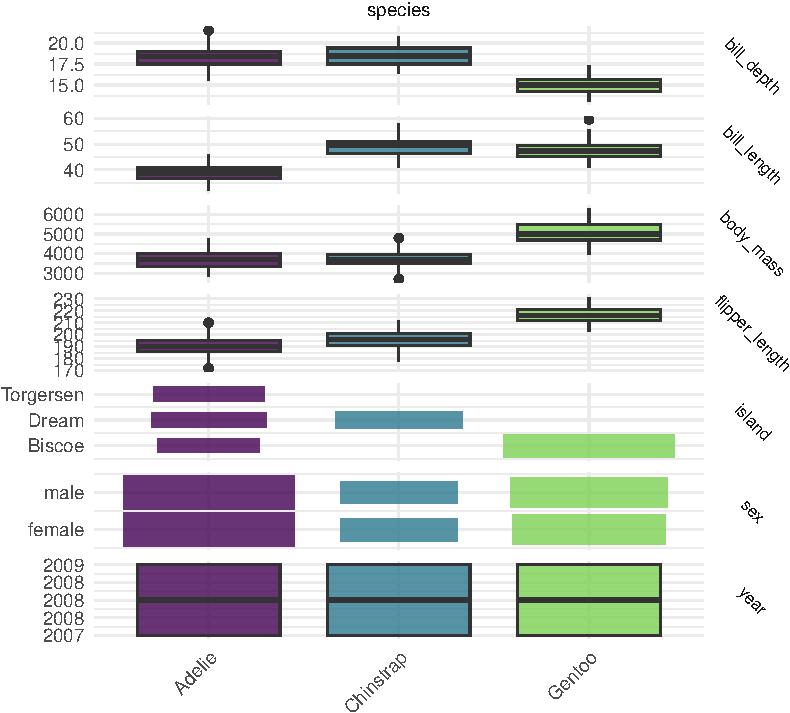
\includegraphics[width=1\textwidth,height=\textheight]{chapters/chapter2/data_and_basic_modeling_files/figure-pdf/fig-penguins-overview-1.pdf}

}

\caption{\label{fig-penguins-overview}Overview of part of the penguins
dataset.}

\end{figure}

\hypertarget{sec-basics-classif-learner}{%
\subsection{LearnerClassif and
MeasureClassif}\label{sec-basics-classif-learner}}

Classification learners, which inherit from
\href{https://mlr3.mlr-org.com/reference/LearnerClassif.html}{\texttt{LearnerClassif}}\index{\texttt{LearnerClassif}}{\marginnote{\begin{footnotesize}\texttt{LearnerClassif}\end{footnotesize}}},
have nearly the same interface as regression learners. However, a key
difference is that the possible predictions in classification are either
\texttt{"response"} -- predicting an observation's class (a penguin's
species in our example, this is sometimes called ``hard labeling'') --
or \texttt{"prob"} -- predicting a vector of probabilities, also called
``posterior probabilities'', of an observation belonging to each class.
In classification, the latter can be more useful as it provides
information about the confidence of the predictions:

\begin{Shaded}
\begin{Highlighting}[]
\NormalTok{lrn\_rpart }\OtherTok{=} \FunctionTok{lrn}\NormalTok{(}\StringTok{"classif.rpart"}\NormalTok{, }\AttributeTok{predict\_type =} \StringTok{"prob"}\NormalTok{)}
\NormalTok{lrn\_rpart}\SpecialCharTok{$}\FunctionTok{train}\NormalTok{(tsk\_penguins, splits}\SpecialCharTok{$}\NormalTok{train)}
\NormalTok{prediction }\OtherTok{=}\NormalTok{ lrn\_rpart}\SpecialCharTok{$}\FunctionTok{predict}\NormalTok{(tsk\_penguins, splits}\SpecialCharTok{$}\NormalTok{test)}
\NormalTok{prediction}
\end{Highlighting}
\end{Shaded}

\begin{verbatim}
<PredictionClassif> for 113 observations:
    row_ids     truth  response prob.Adelie prob.Chinstrap prob.Gentoo
          2    Adelie    Adelie     0.97030         0.0297     0.00000
          4    Adelie    Adelie     0.97030         0.0297     0.00000
          7    Adelie    Adelie     0.97030         0.0297     0.00000
---                                                                   
        338 Chinstrap Chinstrap     0.04651         0.9302     0.02326
        341 Chinstrap    Adelie     0.97030         0.0297     0.00000
        344 Chinstrap Chinstrap     0.04651         0.9302     0.02326
\end{verbatim}

Notice how the predictions include the predicted probabilities for all
three classes, as well as the \texttt{response}, which (by default) is
the class with the highest predicted probability.

Also, the interface for classification measures, which are of class
\href{https://mlr3.mlr-org.com/reference/MeasureClassif.html}{\texttt{MeasureClassif}}\index{\texttt{MeasureClassif}}{\marginnote{\begin{footnotesize}\texttt{MeasureClassif}\end{footnotesize}}},
is identical to regression measures. The key difference in usage is that
you will need to ensure your selected measure evaluates the prediction
type of interest.\index{\texttt{Measure}!\texttt{\$predict\_type}} To
evaluate \texttt{"response"} predictions, you will need measures with
\texttt{predict\_type\ =\ "response"}, or to evaluate probability
predictions you will need \texttt{predict\_type\ =\ "prob"}. The easiest
way to find these measures is by filtering the
\href{https://mlr3.mlr-org.com/reference/mlr_measures.html}{\texttt{mlr\_measures}}
dictionary:

\begin{Shaded}
\begin{Highlighting}[]
\FunctionTok{as.data.table}\NormalTok{(}\FunctionTok{msr}\NormalTok{())[}
\NormalTok{    task\_type }\SpecialCharTok{==} \StringTok{"classif"} \SpecialCharTok{\&}\NormalTok{ predict\_type }\SpecialCharTok{==} \StringTok{"prob"} \SpecialCharTok{\&}
    \SpecialCharTok{!}\FunctionTok{sapply}\NormalTok{(task\_properties, }\ControlFlowTok{function}\NormalTok{(x) }\StringTok{"twoclass"} \SpecialCharTok{\%in\%}\NormalTok{ x)]}
\end{Highlighting}
\end{Shaded}

\begin{verbatim}
                 key                                      label
1:   classif.logloss                                   Log Loss
2: classif.mauc_au1p    Weighted average 1 vs. 1 multiclass AUC
3: classif.mauc_au1u             Average 1 vs. 1 multiclass AUC
4: classif.mauc_aunp Weighted average 1 vs. rest multiclass AUC
5: classif.mauc_aunu          Average 1 vs. rest multiclass AUC
6:    classif.mbrier                     Multiclass Brier Score
4 variables not shown: [task_type, packages, predict_type, task_properties]
\end{verbatim}

We also filtered to remove any measures that have the
\texttt{"twoclass"} property as this would conflict with our
\texttt{"multiclass"} task. We need to use \texttt{sapply} for this, the
\texttt{task\_properties} column is a list column. We can evaluate the
quality of our probability predictions and response predictions
simultaneously by providing multiple measures:

\begin{Shaded}
\begin{Highlighting}[]
\NormalTok{measures }\OtherTok{=} \FunctionTok{msrs}\NormalTok{(}\FunctionTok{c}\NormalTok{(}\StringTok{"classif.mbrier"}\NormalTok{, }\StringTok{"classif.logloss"}\NormalTok{, }\StringTok{"classif.acc"}\NormalTok{))}
\NormalTok{prediction}\SpecialCharTok{$}\FunctionTok{score}\NormalTok{(measures)}
\end{Highlighting}
\end{Shaded}

\begin{verbatim}
 classif.mbrier classif.logloss     classif.acc 
         0.1017          0.2291          0.9469 
\end{verbatim}

The accuracy\index{accuracy} measure evaluates the \texttt{"response"}
predictions whereas the Brier score\index{Brier score}
(\texttt{"classif.mbrier"}, squared difference between predicted
probabilities and the truth) and logloss\index{logloss}
(\texttt{"classif.logloss"}, negative logarithm of the predicted
probability for the true class) are evaluating the probability
predictions.

If no measure is passed to
\texttt{\$score()}\index{\texttt{Prediction}!\texttt{\$score()}}, the
default is the classification error\index{classification error}
(\texttt{msr("classif.ce")}), which is the number of misclassifications
divided by the number of predictions, i.e., \(1 -\)
\texttt{msr("classif.acc")}.

\hypertarget{sec-classif-prediction}{%
\subsection{\texorpdfstring{\texttt{PredictionClassif}, Confusion
Matrix, and
Thresholding}{PredictionClassif, Confusion Matrix, and Thresholding}}\label{sec-classif-prediction}}

\href{https://mlr3.mlr-org.com/reference/PredictionClassif.html}{\texttt{PredictionClassif}}\index{\texttt{PredictionClassif}}{\marginnote{\begin{footnotesize}\texttt{PredictionClassif}\end{footnotesize}}}
objects have two important differences from their regression analog.
Firstly, the added field \texttt{\$confusion}, and secondly the added
method
\texttt{\$set\_threshold()}\index{\texttt{PredictionClassif}!\texttt{\$set\_threshold()}}.

\hypertarget{confusion-matrix}{%
\subsubsection*{Confusion matrix}\label{confusion-matrix}}

A confusion
matrix\index{confusion matrix}{\marginnote{\begin{footnotesize}Confusion
Matrix\end{footnotesize}}} is a popular way to show the quality of
classification (response) predictions in a more detailed fashion by
seeing if a model is good at (mis)classifying observations in a
particular class. For binary and multiclass classification, the
confusion matrix is stored in the
\texttt{\$confusion}\index{\texttt{PredictionClassif}!\texttt{\$confusion}}{\marginnote{\begin{footnotesize}\$confusion\end{footnotesize}}}
field of the
\href{https://mlr3.mlr-org.com/reference/PredictionClassif.html}{\texttt{PredictionClassif}}
object:

\begin{Shaded}
\begin{Highlighting}[]
\NormalTok{prediction}\SpecialCharTok{$}\NormalTok{confusion}
\end{Highlighting}
\end{Shaded}

\begin{verbatim}
           truth
response    Adelie Chinstrap Gentoo
  Adelie        49         3      0
  Chinstrap      1        18      1
  Gentoo         0         1     40
\end{verbatim}

The rows in a confusion matrix are the predicted class and the columns
are the true class. All off-diagonal entries are incorrectly classified
observations, and all diagonal entries are correctly classified. In this
case, the classifier does fairly well classifying all penguins, but we
could have found that it only classifies the Adelie species well but
often conflates Chinstrap and Gentoo, for example.

You can visualize the predicted class labels with
\texttt{autoplot.PredictionClassif()}.

\begin{Shaded}
\begin{Highlighting}[]
\FunctionTok{autoplot}\NormalTok{(prediction)}
\end{Highlighting}
\end{Shaded}

\begin{figure}

{\centering 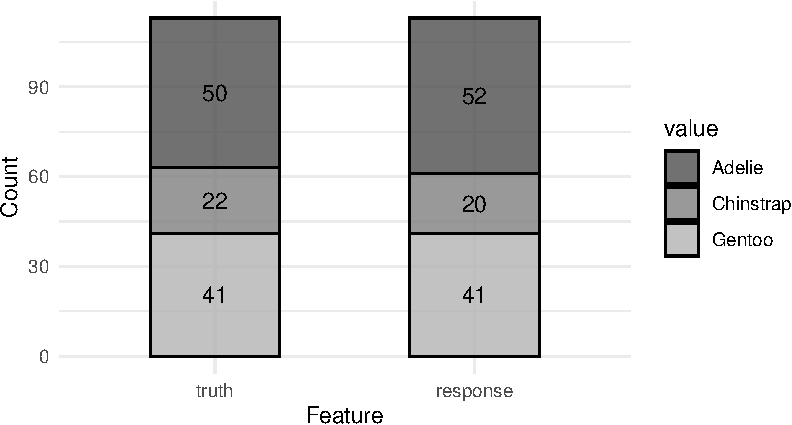
\includegraphics[width=0.7\textwidth,height=\textheight]{chapters/chapter2/data_and_basic_modeling_files/figure-pdf/fig-basics-classlabels-1.pdf}

}

\caption{\label{fig-basics-classlabels}Counts of each class label in the
ground truth data (left) and predictions (right).}

\end{figure}

In the binary classification case, the top left entry corresponds to
true positives\index{true positives}, the top right to false
positives\index{false positives}, the bottom left to false
negatives\index{false negatives} and the bottom right to true
negatives\index{true negatives}. Taking \texttt{tsk\_sonar} as an
example with \texttt{M} as the positive class:

\begin{Shaded}
\begin{Highlighting}[]
\NormalTok{splits }\OtherTok{=} \FunctionTok{partition}\NormalTok{(tsk\_sonar)}
\NormalTok{lrn\_rpart}\SpecialCharTok{$}
  \FunctionTok{train}\NormalTok{(tsk\_sonar, splits}\SpecialCharTok{$}\NormalTok{train)}\SpecialCharTok{$}
  \FunctionTok{predict}\NormalTok{(tsk\_sonar, splits}\SpecialCharTok{$}\NormalTok{test)}\SpecialCharTok{$}
\NormalTok{  confusion}
\end{Highlighting}
\end{Shaded}

\begin{verbatim}
        truth
response  M  R
       M 27 10
       R 10 22
\end{verbatim}

We will return to the concept of binary (mis)classification in greater
detail in Section~\ref{sec-roc}.

\hypertarget{thresholding}{%
\subsubsection*{Thresholding}\label{thresholding}}

The final big difference compared to regression we will discuss is
thresholding\index{thresholding}{\marginnote{\begin{footnotesize}Thresholding\end{footnotesize}}}.
We saw previously that the default \texttt{response} prediction type is
the class with the highest predicted probability. For \texttt{k} classes
with predicted probabilities \(p_1,\dots,p_k\), this is the same as
saying \texttt{response} = argmax\(\{p_1,\dots,p_k\}\). If the maximum
probability is not unique, i.e., multiple classes are predicted to have
the highest probability, then the response is chosen randomly from
these. In binary classification, this means that the positive class will
be selected if the predicted class is greater than 50\%, and the
negative class otherwise.

This 50\% value is known as the threshold and it can be useful to change
this threshold if there is class imbalance (when one class is over- or
under-represented in a dataset), or if there are different costs
associated with classes, or simply if there is a preference to
`over'-predict one class. As an example, let us take
\texttt{tsk("german\_credit")} in which 700 customers have good credit
and 300 have bad. Now we could easily build a model with around ``70\%''
accuracy simply by always predicting a customer will have good credit:

\begin{Shaded}
\begin{Highlighting}[]
\NormalTok{task\_credit }\OtherTok{=} \FunctionTok{tsk}\NormalTok{(}\StringTok{"german\_credit"}\NormalTok{)}
\NormalTok{lrn\_featureless }\OtherTok{=} \FunctionTok{lrn}\NormalTok{(}\StringTok{"classif.featureless"}\NormalTok{, }\AttributeTok{predict\_type =} \StringTok{"prob"}\NormalTok{)}
\NormalTok{split }\OtherTok{=} \FunctionTok{partition}\NormalTok{(task\_credit)}
\NormalTok{lrn\_featureless}\SpecialCharTok{$}\FunctionTok{train}\NormalTok{(task\_credit, split}\SpecialCharTok{$}\NormalTok{train)}
\NormalTok{prediction }\OtherTok{=}\NormalTok{ lrn\_featureless}\SpecialCharTok{$}\FunctionTok{predict}\NormalTok{(task\_credit, split}\SpecialCharTok{$}\NormalTok{test)}
\NormalTok{prediction}\SpecialCharTok{$}\FunctionTok{score}\NormalTok{(}\FunctionTok{msr}\NormalTok{(}\StringTok{"classif.acc"}\NormalTok{))}
\end{Highlighting}
\end{Shaded}

\begin{verbatim}
classif.acc 
        0.7 
\end{verbatim}

\begin{Shaded}
\begin{Highlighting}[]
\FunctionTok{autoplot}\NormalTok{(prediction)}
\end{Highlighting}
\end{Shaded}

\begin{figure}

{\centering 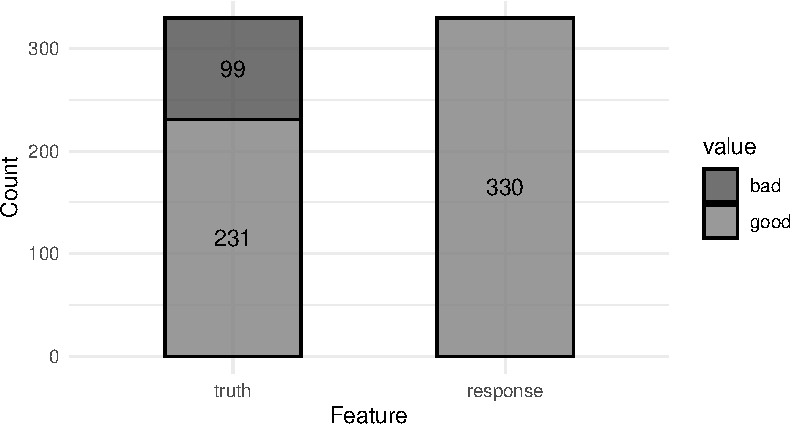
\includegraphics[width=0.7\textwidth,height=\textheight]{chapters/chapter2/data_and_basic_modeling_files/figure-pdf/fig-basics-classlabels-german-1.pdf}

}

\caption{\label{fig-basics-classlabels-german}Class labels ground truth
(left) and predictions (right). The learner completely ignores the `bad'
class.}

\end{figure}

While this model may appear to have good performance on the surface, in
fact, it just ignores all `bad' customers -- this can create big
problems in this finance example, as well as in healthcare tasks and
other settings where false positives\index{false positives} cost more
than false negatives\index{false negatives} (see
Section~\ref{sec-cost-sens} for cost-sensitive classification).

Thresholding allows classes to be selected with a different probability
threshold, so instead of predicting that a customer has bad credit if
P(good) \textless{} 50\%, we might predict bad credit if P(good)
\textless{} 70\% -- notice how we write this in terms of the positive
class, which in this task is `good'. Let us see this in practice:

\begin{Shaded}
\begin{Highlighting}[]
\NormalTok{prediction}\SpecialCharTok{$}\FunctionTok{set\_threshold}\NormalTok{(}\FloatTok{0.7}\NormalTok{)}
\NormalTok{prediction}\SpecialCharTok{$}\FunctionTok{score}\NormalTok{(}\FunctionTok{msr}\NormalTok{(}\StringTok{"classif.acc"}\NormalTok{))}
\end{Highlighting}
\end{Shaded}

\begin{verbatim}
classif.acc 
     0.5394 
\end{verbatim}

\begin{Shaded}
\begin{Highlighting}[]
\NormalTok{lrn\_rpart }\OtherTok{=} \FunctionTok{lrn}\NormalTok{(}\StringTok{"classif.rpart"}\NormalTok{, }\AttributeTok{predict\_type =} \StringTok{"prob"}\NormalTok{)}
\NormalTok{lrn\_rpart}\SpecialCharTok{$}\FunctionTok{train}\NormalTok{(task\_credit, split}\SpecialCharTok{$}\NormalTok{train)}
\NormalTok{prediction }\OtherTok{=}\NormalTok{ lrn\_rpart}\SpecialCharTok{$}\FunctionTok{predict}\NormalTok{(task\_credit, split}\SpecialCharTok{$}\NormalTok{test)}
\NormalTok{prediction}\SpecialCharTok{$}\FunctionTok{score}\NormalTok{(}\FunctionTok{msr}\NormalTok{(}\StringTok{"classif.acc"}\NormalTok{))}
\end{Highlighting}
\end{Shaded}

\begin{verbatim}
classif.acc 
     0.6939 
\end{verbatim}

\begin{Shaded}
\begin{Highlighting}[]
\NormalTok{prediction}\SpecialCharTok{$}\NormalTok{confusion}
\end{Highlighting}
\end{Shaded}

\begin{verbatim}
        truth
response good bad
    good  194  64
    bad    37  35
\end{verbatim}

\begin{Shaded}
\begin{Highlighting}[]
\NormalTok{prediction}\SpecialCharTok{$}\FunctionTok{set\_threshold}\NormalTok{(}\FloatTok{0.7}\NormalTok{)}
\NormalTok{prediction}\SpecialCharTok{$}\FunctionTok{score}\NormalTok{(}\FunctionTok{msr}\NormalTok{(}\StringTok{"classif.acc"}\NormalTok{))}
\end{Highlighting}
\end{Shaded}

\begin{verbatim}
classif.acc 
     0.6879 
\end{verbatim}

\begin{Shaded}
\begin{Highlighting}[]
\NormalTok{prediction}\SpecialCharTok{$}\NormalTok{confusion}
\end{Highlighting}
\end{Shaded}

\begin{verbatim}
        truth
response good bad
    good  181  53
    bad    50  46
\end{verbatim}

While our model performs `worse' overall, i.e.~with lower accuracy, it
is still a `better' model as it more accurately captures the
relationship between classes.

In the binary classification setting, \texttt{\$set\_threshold()} only
requires one numeric argument, which corresponds with the threshold for
the positive class -- hence it is essential to ensure the positive class
is correctly set in your task.

In multiclass classification, thresholding works by first assigning a
threshold to each of the \texttt{n} classes, dividing the predicted
probabilities for each class by these thresholds to return \texttt{n}
ratios, and then the class with the highest ratio is selected. For
example, say we are predicting if a new observation will be of class A,
B, C, or D and we have predicted
\(P(A = 0.2), P(B = 0.4), P(C = 0.1), P(D = 0.3)\). We will assume that
the threshold for all classes is identical and \texttt{1}:

\begin{Shaded}
\begin{Highlighting}[]
\NormalTok{probs }\OtherTok{=} \FunctionTok{c}\NormalTok{(}\FloatTok{0.2}\NormalTok{, }\FloatTok{0.4}\NormalTok{, }\FloatTok{0.1}\NormalTok{, }\FloatTok{0.3}\NormalTok{)}
\NormalTok{thresholds }\OtherTok{=} \FunctionTok{c}\NormalTok{(}\AttributeTok{A =} \DecValTok{1}\NormalTok{, }\AttributeTok{B =} \DecValTok{1}\NormalTok{, }\AttributeTok{C =} \DecValTok{1}\NormalTok{, }\AttributeTok{D =} \DecValTok{1}\NormalTok{)}
\NormalTok{probs}\SpecialCharTok{/}\NormalTok{thresholds}
\end{Highlighting}
\end{Shaded}

\begin{verbatim}
  A   B   C   D 
0.2 0.4 0.1 0.3 
\end{verbatim}

We would therefore predict our observation is of class B as this is the
highest ratio. However, we could change our thresholds so that D has the
lowest threshold and is most likely to be predicted, A has the highest
threshold, and B and C have equal thresholds:

\begin{Shaded}
\begin{Highlighting}[]
\NormalTok{thresholds }\OtherTok{=} \FunctionTok{c}\NormalTok{(}\AttributeTok{A =} \FloatTok{0.5}\NormalTok{, }\AttributeTok{B =} \FloatTok{0.25}\NormalTok{, }\AttributeTok{C =} \FloatTok{0.25}\NormalTok{, }\AttributeTok{D =} \FloatTok{0.1}\NormalTok{)}
\NormalTok{probs}\SpecialCharTok{/}\NormalTok{thresholds}
\end{Highlighting}
\end{Shaded}

\begin{verbatim}
  A   B   C   D 
0.4 1.6 0.4 3.0 
\end{verbatim}

Now our observation will be predicted to be in class D.

In \texttt{mlr3}, this is achieved by passing a named list to
\texttt{\$set\_threshold()}. This is demonstrated below with
\texttt{tsk("zoo")}. Before changing the thresholds, some classes are
never predicted and some are predicted more often than they occur.

\begin{Shaded}
\begin{Highlighting}[]
\FunctionTok{library}\NormalTok{(ggplot2)}
\FunctionTok{library}\NormalTok{(patchwork)}

\NormalTok{tsk\_zoo }\OtherTok{=} \FunctionTok{tsk}\NormalTok{(}\StringTok{"zoo"}\NormalTok{)}
\NormalTok{splits }\OtherTok{=} \FunctionTok{partition}\NormalTok{(tsk\_zoo)}
\NormalTok{lrn\_rpart }\OtherTok{=} \FunctionTok{lrn}\NormalTok{(}\StringTok{"classif.rpart"}\NormalTok{, }\AttributeTok{predict\_type =} \StringTok{"prob"}\NormalTok{)}
\NormalTok{lrn\_rpart}\SpecialCharTok{$}\FunctionTok{train}\NormalTok{(tsk\_zoo, splits}\SpecialCharTok{$}\NormalTok{train)}
\NormalTok{prediction }\OtherTok{=}\NormalTok{ lrn\_rpart}\SpecialCharTok{$}\FunctionTok{predict}\NormalTok{(tsk\_zoo, splits}\SpecialCharTok{$}\NormalTok{test)}
\NormalTok{before }\OtherTok{=} \FunctionTok{autoplot}\NormalTok{(prediction) }\SpecialCharTok{+} \FunctionTok{ggtitle}\NormalTok{(}\StringTok{"Default thresholds"}\NormalTok{)}
\NormalTok{new\_thresh }\OtherTok{=} \FunctionTok{proportions}\NormalTok{(}\FunctionTok{table}\NormalTok{(tsk\_zoo}\SpecialCharTok{$}\FunctionTok{truth}\NormalTok{(splits}\SpecialCharTok{$}\NormalTok{train)))}
\NormalTok{new\_thresh}
\end{Highlighting}
\end{Shaded}

\begin{verbatim}

       mammal          bird       reptile          fish     amphibian 
      0.40299       0.19403       0.04478       0.13433       0.04478 
       insect mollusc.et.al 
      0.07463       0.10448 
\end{verbatim}

\begin{Shaded}
\begin{Highlighting}[]
\NormalTok{prediction}\SpecialCharTok{$}\FunctionTok{set\_threshold}\NormalTok{(new\_thresh)}
\NormalTok{after }\OtherTok{=} \FunctionTok{autoplot}\NormalTok{(prediction) }\SpecialCharTok{+} \FunctionTok{ggtitle}\NormalTok{(}\StringTok{"Inverse weighting thresholds"}\NormalTok{)}
\NormalTok{before }\SpecialCharTok{+}\NormalTok{ after }\SpecialCharTok{+} \FunctionTok{plot\_layout}\NormalTok{(}\AttributeTok{guides =} \StringTok{"collect"}\NormalTok{)}
\end{Highlighting}
\end{Shaded}

\begin{figure}[H]

{\centering 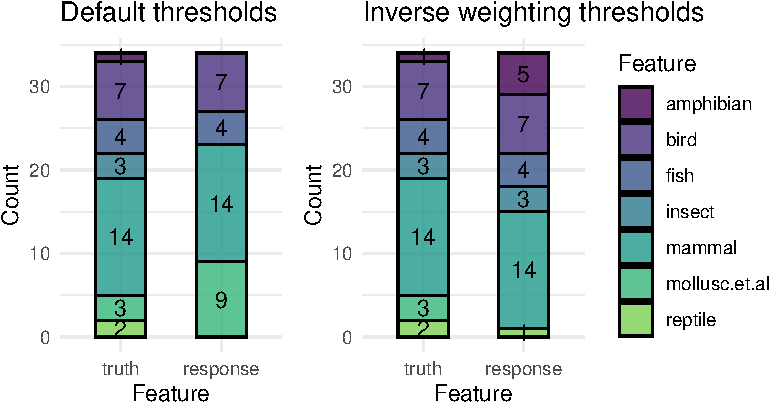
\includegraphics[width=1\textwidth,height=\textheight]{chapters/chapter2/data_and_basic_modeling_files/figure-pdf/fig-zoopreds-1.pdf}

}

\caption{\label{fig-zoopreds}Comparing predicted and ground truth values
for the zoo dataset.}

\end{figure}

Again we see that the model better represents all classes after
thresholding. In this example we set the new thresholds to be the
proportions of each class in the training set. This is known as inverse
weighting\index{inverse weighting}, as we divide the predicted
probability by these class proportions before we select the label with
the highest ratio.

In Section~\ref{sec-cost-sens} we will look at cost-sensitive
classification\index{classification!cost-sensitive} where each cell in
the confusion matrix has a different associated cost.

\hypertarget{sec-row-col-roles}{%
\section{Task Column Roles}\label{sec-row-col-roles}}

\begin{tcolorbox}[enhanced jigsaw, colframe=quarto-callout-note-color-frame, rightrule=.15mm, bottomrule=.15mm, toprule=.15mm, opacityback=0, colback=white, left=2mm, arc=.35mm, breakable, leftrule=.75mm]
\begin{minipage}[t]{5.5mm}
\textcolor{quarto-callout-note-color}{\faInfo}
\end{minipage}%
\begin{minipage}[t]{\textwidth - 5.5mm}

\textbf{This section covers advanced ML or technical
details.}\vspace{2mm}

\end{minipage}%
\end{tcolorbox}

Now that we have covered regression and classification, we will briefly
return to tasks and in particular to column roles\index{column roles},
which are used to customize tasks further. Column roles are used by
\texttt{Task} objects to define important metadata that can be used by
learners and other objects to interact with the task. True to their
name, they assign particular roles to columns in the data, we have
already seen some of these in action with targets and features. There
are seven column roles:

\begin{enumerate}
\def\labelenumi{\arabic{enumi}.}
\tightlist
\item
  \texttt{"feature"}: Features used for prediction.
\item
  \texttt{"target"}: Target variable to predict.
\item
  \texttt{"name"}: Row names/observation labels, e.g., for
  \texttt{mtcars} this is the \texttt{"model"} column.
\item
  \texttt{"order"}: Variable(s) used to order data returned by
  \texttt{\$data()}; must be sortable with \texttt{order()}.
\item
  \texttt{"group"}: Variable used to keep observations together during
  resampling.
\item
  \texttt{"stratum"}: Variable(s) to stratify during resampling.
\item
  \texttt{"weight"}: Observation weights. Only one numeric column may
  have this role.
\end{enumerate}

We have already seen how features and targets work in
Section~\ref{sec-tasks}, which are the only column roles that each task
must have. In Section~\ref{sec-strat-group} we will have a look at the
\texttt{stratum} and \texttt{group} column roles. So, for now, we will
only look at \texttt{order}, and \texttt{weight}. We will not go into
detail about \texttt{name}, which is primarily used in plotting and will
almost always be the \texttt{rownames()} of the underlying data.

Column roles are updated using
\texttt{\$set\_col\_roles()}\index{\texttt{Task}!\texttt{\$set\_col\_roles()}}.
When we set the \texttt{"order"} column role, the data is ordered
according to that column(s). In the following example, we set the
\texttt{"order"} column role and then order data by this column by
including \texttt{ordered\ =\ TRUE}:

\begin{Shaded}
\begin{Highlighting}[]
\NormalTok{df }\OtherTok{=} \FunctionTok{data.frame}\NormalTok{(mtcars[}\DecValTok{1}\SpecialCharTok{:}\DecValTok{2}\NormalTok{, ], }\AttributeTok{idx =} \DecValTok{2}\SpecialCharTok{:}\DecValTok{1}\NormalTok{)}
\NormalTok{tsk\_mtcars\_order }\OtherTok{=} \FunctionTok{as\_task\_regr}\NormalTok{(df, }\AttributeTok{target =} \StringTok{"mpg"}\NormalTok{)}
\CommentTok{\# original order}
\NormalTok{tsk\_mtcars\_order}\SpecialCharTok{$}\FunctionTok{data}\NormalTok{(}\AttributeTok{ordered =} \ConstantTok{TRUE}\NormalTok{)}
\end{Highlighting}
\end{Shaded}

\begin{verbatim}
   mpg am carb cyl disp drat gear  hp idx  qsec vs    wt
1:  21  1    4   6  160  3.9    4 110   2 16.46  0 2.620
2:  21  1    4   6  160  3.9    4 110   1 17.02  0 2.875
\end{verbatim}

\begin{Shaded}
\begin{Highlighting}[]
\CommentTok{\# order by "idx" column}
\NormalTok{tsk\_mtcars\_order}\SpecialCharTok{$}\FunctionTok{set\_col\_roles}\NormalTok{(}\StringTok{"idx"}\NormalTok{, }\AttributeTok{roles =} \StringTok{"order"}\NormalTok{)}
\NormalTok{tsk\_mtcars\_order}\SpecialCharTok{$}\FunctionTok{data}\NormalTok{(}\AttributeTok{ordered =} \ConstantTok{TRUE}\NormalTok{)}
\end{Highlighting}
\end{Shaded}

\begin{verbatim}
   mpg am carb cyl disp drat gear  hp  qsec vs    wt
1:  21  1    4   6  160  3.9    4 110 17.02  0 2.875
2:  21  1    4   6  160  3.9    4 110 16.46  0 2.620
\end{verbatim}

In this example we can see that by setting \texttt{"idx"} to have the
\texttt{"order"} column role, it is no longer used as a feature when we
run \texttt{\$data()} but instead is used to order the observations
according to its value. This metadata is not passed to a learner.

The \texttt{weights} column role is used to weight data points
differently. One example of why we would do this is in classification
tasks with severe class imbalance, where weighting the minority class
more heavily may improve the model's predictive performance for that
class. For example in the \texttt{breast\_cancer} dataset, there are
more instances of benign tumors than malignant tumors, so if we want to
better predict malignant tumors we could weight the data in favor of
this class:

\begin{Shaded}
\begin{Highlighting}[]
\NormalTok{cancer\_unweighted }\OtherTok{=} \FunctionTok{tsk}\NormalTok{(}\StringTok{"breast\_cancer"}\NormalTok{)}
\FunctionTok{summary}\NormalTok{(cancer\_unweighted}\SpecialCharTok{$}\FunctionTok{data}\NormalTok{()}\SpecialCharTok{$}\NormalTok{class)}
\end{Highlighting}
\end{Shaded}

\begin{verbatim}
malignant    benign 
      239       444 
\end{verbatim}

\begin{Shaded}
\begin{Highlighting}[]
\CommentTok{\# add column where weight is 2 if class "malignant", and 1 otherwise}
\NormalTok{df }\OtherTok{=}\NormalTok{ cancer\_unweighted}\SpecialCharTok{$}\FunctionTok{data}\NormalTok{()}
\NormalTok{df}\SpecialCharTok{$}\NormalTok{weights }\OtherTok{=} \FunctionTok{ifelse}\NormalTok{(df}\SpecialCharTok{$}\NormalTok{class }\SpecialCharTok{==} \StringTok{"malignant"}\NormalTok{, }\DecValTok{2}\NormalTok{, }\DecValTok{1}\NormalTok{)}

\CommentTok{\# create new task and role}
\NormalTok{cancer\_weighted }\OtherTok{=} \FunctionTok{as\_task\_classif}\NormalTok{(df, }\AttributeTok{target =} \StringTok{"class"}\NormalTok{)}
\NormalTok{cancer\_weighted}\SpecialCharTok{$}\FunctionTok{set\_col\_roles}\NormalTok{(}\StringTok{"weights"}\NormalTok{, }\AttributeTok{roles =} \StringTok{"weight"}\NormalTok{)}

\CommentTok{\# compare weighted and unweighted predictions}
\NormalTok{split }\OtherTok{=} \FunctionTok{partition}\NormalTok{(cancer\_unweighted)}
\NormalTok{lrn\_rf }\OtherTok{=} \FunctionTok{lrn}\NormalTok{(}\StringTok{"classif.ranger"}\NormalTok{)}
\NormalTok{lrn\_rf}\SpecialCharTok{$}\FunctionTok{train}\NormalTok{(cancer\_unweighted, split}\SpecialCharTok{$}\NormalTok{train)}\SpecialCharTok{$}
  \FunctionTok{predict}\NormalTok{(cancer\_unweighted, split}\SpecialCharTok{$}\NormalTok{test)}\SpecialCharTok{$}\FunctionTok{score}\NormalTok{()}
\end{Highlighting}
\end{Shaded}

\begin{verbatim}
classif.ce 
    0.0177 
\end{verbatim}

\begin{Shaded}
\begin{Highlighting}[]
\NormalTok{lrn\_rf}\SpecialCharTok{$}\FunctionTok{train}\NormalTok{(cancer\_weighted, split}\SpecialCharTok{$}\NormalTok{train)}\SpecialCharTok{$}
  \FunctionTok{predict}\NormalTok{(cancer\_weighted, split}\SpecialCharTok{$}\NormalTok{test)}\SpecialCharTok{$}\FunctionTok{score}\NormalTok{()}
\end{Highlighting}
\end{Shaded}

\begin{verbatim}
classif.ce 
   0.00885 
\end{verbatim}

In this example, weighting improves the overall model performance (but
see Chapter~\ref{sec-performance} for more thorough comparison methods).
Not all models can handle weights in tasks so check a learner's
properties to make sure this column role is being used as expected.

\hypertarget{sec-lrns-add}{%
\section{Supported Learning Algorithms}\label{sec-lrns-add}}

\texttt{mlr3} supports many learning algorithms (some with multiple
implementations) as \texttt{Learner}s. These are primarily provided by
the \href{https://mlr3.mlr-org.com}{\texttt{mlr3}}\index{\texttt{mlr3}},
\href{https://mlr3learners.mlr-org.com}{\texttt{mlr3learners}}\index{\texttt{mlr3learners}}
and
\href{https://mlr3extralearners.mlr-org.com}{\texttt{mlr3extralearners}}\index{\texttt{mlr3extralearners}}
packages. However, all packages that implement new tasks
(Chapter~\ref{sec-special}) also include a handful of simple algorithms.

The list of learners included in \texttt{mlr3} is deliberately small to
avoid large sets of dependencies:

\begin{itemize}
\tightlist
\item
  Featureless learners
  (\texttt{"regr.featureless"}/\texttt{"classif.featureless"}), which
  are baseline learners (Section~\ref{sec-basics-featureless}).
\item
  Debug learners (\texttt{"regr.debug"}/\texttt{"classif.debug"}), which
  are used to debug code (Section~\ref{sec-error-handling}).
\item
  Classification and regression trees (also known as CART:
  \texttt{"regr.rpart"}/\texttt{"classif.rpart"}).
\end{itemize}

The
\href{https://mlr3learners.mlr-org.com}{\texttt{mlr3learners}}\index{\texttt{mlr3learners}}
package contains a selection of algorithms (and select implementations)
chosen by the mlr team that we recommend as a good starting point for
most experiments:

\begin{itemize}
\tightlist
\item
  Linear (\texttt{"regr.lm"}) and logistic (\texttt{"classif.log\_reg"})
  regression\index{logistic regression}.
\item
  Penalized generalized linear models, where the penalization is either
  exposed as a hyperparameter
  (\texttt{"regr.glmnet"}/\texttt{"classif.glmnet"})\index{generalized linear model}
  or where it is optimized automatically
  (\texttt{"regr.cv\_glmnet"}/\texttt{"classif.cv\_glmnet"}).
\item
  Weighted \(k\)-Nearest Neighbors\index{k-nearest neighbors}
  (\texttt{"regr.kknn"}/\texttt{"classif.kknn"}).
\item
  Kriging / Gaussian process\index{Gaussian process} regression
  (\texttt{"regr.km"}).
\item
  Linear (\texttt{"classif.lda"}) and quadratic (\texttt{"classif.qda"})
  discriminant analysis.
\item
  Naïve Bayes classification (\texttt{"classif.naive\_bayes"}).
\item
  Support-vector machines\index{support vector machine}
  (\texttt{"regr.svm"}/\texttt{"classif.svm"}).
\item
  Gradient boosting\index{boosting}
  (\texttt{"regr.xgboost"}/\texttt{"classif.xgboost"}).
\item
  Random forests\index{random forest} for regression and classification
  (\texttt{"regr.ranger"}/\texttt{"classif.ranger"}).
\end{itemize}

The majority of other supported learners are in
\href{https://mlr3extralearners.mlr-org.com}{\texttt{mlr3extralearners}}\index{\texttt{mlr3extralearners}}.
You can find an up-to-date list of learners at
\url{https://mlr-org.com/learners.html}.

The dictionary
\href{https://mlr3.mlr-org.com/reference/mlr_learners.html}{\texttt{mlr\_learners}}\index{\texttt{mlr\_learners}}
contains learners that are supported in loaded packages:

\begin{Shaded}
\begin{Highlighting}[]
\NormalTok{learners\_dt }\OtherTok{=} \FunctionTok{as.data.table}\NormalTok{(mlr\_learners)}
\NormalTok{learners\_dt}
\end{Highlighting}
\end{Shaded}

\begin{verbatim}
                     key                       label task_type
  1:  classif.AdaBoostM1           Adaptive Boosting   classif
  2:         classif.C50            Tree-based Model   classif
  3:         classif.IBk           Nearest Neighbour   classif
  4:         classif.J48            Tree-based Model   classif
  5:        classif.JRip Propositional Rule Learner.   classif
 ---                                                          
134: surv.priority_lasso              Priority Lasso      surv
135:         surv.ranger               Random Forest      surv
136:          surv.rfsrc               Random Forest      surv
137:            surv.svm      Support Vector Machine      surv
138:        surv.xgboost           Gradient Boosting      surv
4 variables not shown: [feature_types, packages, properties, predict_types]
\end{verbatim}

The resulting \texttt{data.table} contains a lot of metadata that is
useful for identifying learners with particular properties. For example,
we can list all learners that support classification problems:

\begin{Shaded}
\begin{Highlighting}[]
\NormalTok{learners\_dt[task\_type }\SpecialCharTok{==} \StringTok{"classif"}\NormalTok{]}
\end{Highlighting}
\end{Shaded}

\begin{verbatim}
                   key                       label task_type
 1: classif.AdaBoostM1           Adaptive Boosting   classif
 2:        classif.C50            Tree-based Model   classif
 3:        classif.IBk           Nearest Neighbour   classif
 4:        classif.J48            Tree-based Model   classif
 5:       classif.JRip Propositional Rule Learner.   classif
---                                                         
40:     classif.ranger                        <NA>   classif
41:      classif.rfsrc               Random Forest   classif
42:      classif.rpart         Classification Tree   classif
43:        classif.svm                        <NA>   classif
44:    classif.xgboost                        <NA>   classif
4 variables not shown: [feature_types, packages, properties, predict_types]
\end{verbatim}

We can filter by multiple conditions, for example to list all regression
learners that can predict standard errors:

\begin{Shaded}
\begin{Highlighting}[]
\NormalTok{learners\_dt[task\_type }\SpecialCharTok{==} \StringTok{"regr"} \SpecialCharTok{\&}
  \FunctionTok{sapply}\NormalTok{(predict\_types, }\ControlFlowTok{function}\NormalTok{(x) }\StringTok{"se"} \SpecialCharTok{\%in\%}\NormalTok{ x)]}
\end{Highlighting}
\end{Shaded}

\begin{verbatim}
                key                                    label task_type
1:       regr.debug             Debug Learner for Regression      regr
2:       regr.earth Multivariate Adaptive Regression Splines      regr
3: regr.featureless           Featureless Regression Learner      regr
4:         regr.gam    Generalized Additive Regression Model      regr
5:         regr.glm            Generalized Linear Regression      regr
6:          regr.km                                     <NA>      regr
7:          regr.lm                                     <NA>      regr
8:         regr.mob       Model-based Recursive Partitioning      regr
9:      regr.ranger                                     <NA>      regr
4 variables not shown: [feature_types, packages, properties, predict_types]
\end{verbatim}

\hypertarget{conclusion}{%
\section{Conclusion}\label{conclusion}}

In this chapter, we covered the building blocks of
\href{https://mlr3.mlr-org.com}{\texttt{mlr3}}\index{\texttt{mlr3}}. We
first introduced basic ML methodology and then showed how this is
implemented in \texttt{mlr3}. We began by looking at the
\href{https://mlr3.mlr-org.com/reference/Task.html}{\texttt{Task}}
class, which is used to define machine learning tasks or problems to
solve. We then looked at the
\href{https://mlr3.mlr-org.com/reference/Learner.html}{\texttt{Learner}}
class, which encapsulates machine learning algorithms, hyperparameters,
and other meta-information. Finally, we considered how to evaluate
machine learning models with objects from the
\href{https://mlr3.mlr-org.com/reference/Measure.html}{\texttt{Measure}}
class. After looking at regression implementations, we extended all the
above to the classification setting, before finally looking at some
extra details about tasks and the learning algorithms that are
implemented across \texttt{mlr3}. The rest of this book will build on
the basic elements seen in this chapter, starting with more advanced
model comparison methods in Chapter~\ref{sec-performance} before moving
on to improve model performance with automated hyperparameter tuning in
Chapter~\ref{sec-optimization}.

\hypertarget{tbl-basics-api}{}
\begin{longtable}[]{@{}
  >{\raggedright\arraybackslash}p{(\columnwidth - 4\tabcolsep) * \real{0.2143}}
  >{\raggedright\arraybackslash}p{(\columnwidth - 4\tabcolsep) * \real{0.3571}}
  >{\raggedright\arraybackslash}p{(\columnwidth - 4\tabcolsep) * \real{0.4286}}@{}}
\caption{\label{tbl-basics-api}Important classes and functions covered
in this chapter with underlying class (if applicable), class constructor
or function, and important class fields and methods (if
applicable).}\tabularnewline
\toprule\noalign{}
\begin{minipage}[b]{\linewidth}\raggedright
Class
\end{minipage} & \begin{minipage}[b]{\linewidth}\raggedright
Constructor/Function
\end{minipage} & \begin{minipage}[b]{\linewidth}\raggedright
Fields/Methods
\end{minipage} \\
\midrule\noalign{}
\endfirsthead
\toprule\noalign{}
\begin{minipage}[b]{\linewidth}\raggedright
Class
\end{minipage} & \begin{minipage}[b]{\linewidth}\raggedright
Constructor/Function
\end{minipage} & \begin{minipage}[b]{\linewidth}\raggedright
Fields/Methods
\end{minipage} \\
\midrule\noalign{}
\endhead
\bottomrule\noalign{}
\endlastfoot
\href{https://mlr3.mlr-org.com/reference/Task.html}{\texttt{Task}} &
\href{https://mlr3.mlr-org.com/reference/mlr_sugar.html}{\texttt{tsk()}}/\href{https://mlr3.mlr-org.com/reference/mlr_sugar.html}{\texttt{tsks()}}/\texttt{as\_task\_X}
& \texttt{\$filter()}; \texttt{\$select()}; \texttt{\$data()} \\
\href{https://mlr3.mlr-org.com/reference/Learner.html}{\texttt{Learner}}
&
\href{https://mlr3.mlr-org.com/reference/mlr_sugar.html}{\texttt{lrn()}}/\href{https://mlr3.mlr-org.com/reference/mlr_sugar.html}{\texttt{lrns()}}
& \texttt{\$train()}; \texttt{\$predict()};
\texttt{\$predict\_newdata()}; \texttt{\$model()} \\
\href{https://mlr3.mlr-org.com/reference/Prediction.html}{\texttt{Prediction}}
& \texttt{some\_learner\$predict()} & \texttt{\$score()};
\texttt{\$set\_threshold()}; \texttt{\$confusion} \\
\href{https://mlr3.mlr-org.com/reference/Measure.html}{\texttt{Measure}}
&
\href{https://mlr3.mlr-org.com/reference/mlr_sugar.html}{\texttt{msr()}}/\href{https://mlr3.mlr-org.com/reference/mlr_sugar.html}{\texttt{msrs()}}
& - \\
\end{longtable}

\hypertarget{exercises}{%
\section{Exercises}\label{exercises}}

\begin{enumerate}
\def\labelenumi{\arabic{enumi}.}
\tightlist
\item
  Train a classification model with the \texttt{classif.rpart} learner
  on the ``Pima Indians Diabetes'' dataset. Do this without using
  \texttt{tsk("pima")}, and instead by constructing a task from the
  dataset in the \texttt{mlbench}-package:
  \texttt{data(PimaIndiansDiabetes2,\ package\ =\ "mlbench")}. Make sure
  to define the \texttt{pos} outcome as positive class. Train the model
  on a random 80\% subset of the given data and evaluate its performance
  with the classification error measure on the remaining data. (Note
  that the data set has NAs in its features. You can either rely on
  \texttt{rpart}`s capability to handle them internally ('surrogate
  splits') or remove them from the initial \texttt{data.frame} by using
  \texttt{na.omit}.
\item
  Calculate the true positive, false positive, true negative, and false
  negative rates of the predictions made by the model in Exercise 1. Try
  to solve this in two ways: (a) Using \texttt{mlr3measures}-predefined
  measure objects, and (b) without using \texttt{mlr3} tools by directly
  working on the ground truth and prediction vectors. Compare the
  results.
\item
  Change the threshold of the model from Exercise 1 such that the false
  positive rate is lower than the false negative rate. What is one
  reason you might do this in practice?
\end{enumerate}

\hypertarget{sec-performance}{%
\chapter{Evaluation and Benchmarking}\label{sec-performance}}

\vspace{-15mm}\addtocontents{toc}{\textit{Giuseppe Casalicchio and Lukas Burk}}

\textbf{Giuseppe Casalicchio} \newline 
\emph{Ludwig-Maximilians-Universität München, and Munich Center for
Machine Learning (MCML), and Essential Data Science Training GmbH}

\textbf{Lukas Burk} \newline  \emph{Ludwig-Maximilians-Universität
München, and Leibniz Institute for Prevention Research and Epidemiology
- BIPS, and Munich Center for Machine Learning (MCML)}
\newline \newline 

A supervised machine learning model can only be deployed in practice if
it has a good generalization
performance\index{generalization performance}{\marginnote{\begin{footnotesize}Generalization
Performance\end{footnotesize}}}, which means it generalizes well to new,
unseen data. Accurate estimation of the generalization performance is
crucial for many aspects of machine learning application and research --
whether we want to fairly compare a novel algorithm with established
ones or to find the best algorithm for a particular task. The concept of
performance estimation\index{performance estimation} provides
information on how well a model will generalize to new data and plays an
important role in the context of model comparison
(Section~\ref{sec-benchmarking}), model selection, and hyperparameter
tuning (Chapter~\ref{sec-optimization}).

Assessing the generalization performance of a model begins with
selecting a performance measure\index{performance measure} that is
appropriate for our given task and evaluation goal. As we have seen in
Section~\ref{sec-eval}, performance measures typically compute a numeric
score indicating how well the model predictions match the ground truth
(though some technical measures were seen in
Section~\ref{sec-basics-measures-tech}). Once we have decided on a
performance measure, the next step is to adopt a strategy that defines
how to use the available data to estimate the generalization
performance. Using the same data to train and test a model is a bad
strategy as it would lead to an overly optimistic performance estimate.
For example, a model that is overfitted (fit too closely to the data)
could make perfect predictions on training data simply by memorizing it
and then only make random guesses for new data. In
Section~\ref{sec-basics-partition} we introduced
\href{https://mlr3.mlr-org.com/reference/partition.html}{\texttt{partition()}},
which splits a dataset into training data\index{training data} -- data
for training the model -- and test data\index{test data} -- data for
testing the model and estimating the generalization performance, this is
known as the holdout strategy (Section~\ref{sec-holdout-scoring}) and is
where we will begin this chapter. We will then consider more advanced
strategies for assessing the generalization performance
(Section~\ref{sec-resampling}), look at robust methods for comparing
models (Section~\ref{sec-benchmarking}), and finally will discuss
specialized performance measures for binary classification
(Section~\ref{sec-roc}). For an in-depth overview of measures and
performance estimation, we recommend Japkowicz and Shah (2011).

\begin{tcolorbox}[enhanced jigsaw, opacitybacktitle=0.6, rightrule=.15mm, opacityback=0, arc=.35mm, breakable, titlerule=0mm, colframe=quarto-callout-warning-color-frame, coltitle=black, bottomrule=.15mm, toprule=.15mm, colback=white, colbacktitle=quarto-callout-warning-color!10!white, bottomtitle=1mm, toptitle=1mm, title=\textcolor{quarto-callout-warning-color}{\faExclamationTriangle}\hspace{0.5em}{Resampling Does Not Avoid Model Overfitting}, leftrule=.75mm, left=2mm]

A common \textbf{misunderstanding} is that holdout and other more
advanced resampling strategies can prevent model overfitting. In fact,
these methods just make overfitting visible as we can separately
evaluate train/test performance. Resampling strategies also allow us to
make (nearly) unbiased estimations of the generalization error.

\end{tcolorbox}

\hypertarget{sec-holdout-scoring}{%
\section{Holdout and Scoring}\label{sec-holdout-scoring}}

An important goal of ML is to learn a model that can then be used to
make predictions about new data. For this model to be as accurate as
possible, we would ideally train it on as much data as is available.
However, data is limited and as we have discussed we cannot train and
test a model on the same data. In practice, one would usually create an
intermediate
model\index{intermediate model}{\marginnote{\begin{footnotesize}Intermediate
Model\end{footnotesize}}}, which is trained on a subset of the available
data and then tested on the remainder of the data. The performance of
this intermediate model, obtained by comparing the model predictions to
the ground truth, is an estimate of the generalization performance of
the final model, which is the model fitted on all data.

The
holdout\index{holdout}{\marginnote{\begin{footnotesize}Holdout\end{footnotesize}}}
strategy is a simple method to create this split between training and
testing datasets, whereby the original data is split into two datasets
using a defined ratio. Ideally, the training dataset should be as large
as possible so the intermediate model represents the final model as well
possible. If the training data is too small, the intermediate model is
unlikely to perform as well as the final model, resulting in a
pessimistically biased performance estimate. On the other hand, if the
training data is too large, then we will not have a reliable estimate of
the generalization performance due to high variance resulting from small
test data. As a rule of thumb, it is common to use 2/3 of the data for
training and 1/3 for testing as this provides a reasonable trade-off
between bias and variance of the generalization performance estimate
(Kohavi 1995; Dobbin and Simon 2011).

In Chapter~\ref{sec-basics}, we used
\href{https://mlr3.mlr-org.com/reference/partition.html}{\texttt{partition()}}
to apply the holdout method to a
\href{https://mlr3.mlr-org.com/reference/Task.html}{\texttt{Task}}
object. To recap, let us split \texttt{tsk("penguins")} with a 2/3
holdout (default split):

\begin{Shaded}
\begin{Highlighting}[]
\NormalTok{tsk\_penguins }\OtherTok{=} \FunctionTok{tsk}\NormalTok{(}\StringTok{"penguins"}\NormalTok{)}
\NormalTok{splits }\OtherTok{=} \FunctionTok{partition}\NormalTok{(tsk\_penguins)}
\NormalTok{lrn\_rpart }\OtherTok{=} \FunctionTok{lrn}\NormalTok{(}\StringTok{"classif.rpart"}\NormalTok{)}
\NormalTok{lrn\_rpart}\SpecialCharTok{$}\FunctionTok{train}\NormalTok{(tsk\_penguins, splits}\SpecialCharTok{$}\NormalTok{train)}
\NormalTok{prediction }\OtherTok{=}\NormalTok{ lrn\_rpart}\SpecialCharTok{$}\FunctionTok{predict}\NormalTok{(tsk\_penguins, splits}\SpecialCharTok{$}\NormalTok{test)}
\end{Highlighting}
\end{Shaded}

We can now estimate the generalization performance of a final model by
evaluating the quality of the predictions from our intermediate model.
As we have seen in Section~\ref{sec-eval}, this is simply a case of
choosing one or more measures and passing them to the \texttt{\$score()}
function. So to estimate the accuracy of our final model we would pass
the accuracy measure to our intermediate model:

\begin{Shaded}
\begin{Highlighting}[]
\NormalTok{prediction}\SpecialCharTok{$}\FunctionTok{score}\NormalTok{(}\FunctionTok{msr}\NormalTok{(}\StringTok{"classif.acc"}\NormalTok{))}
\end{Highlighting}
\end{Shaded}

\begin{verbatim}
classif.acc 
     0.9558 
\end{verbatim}

\begin{tcolorbox}[enhanced jigsaw, opacitybacktitle=0.6, rightrule=.15mm, opacityback=0, arc=.35mm, breakable, titlerule=0mm, colframe=quarto-callout-tip-color-frame, coltitle=black, bottomrule=.15mm, toprule=.15mm, colback=white, colbacktitle=quarto-callout-tip-color!10!white, bottomtitle=1mm, toptitle=1mm, title=\textcolor{quarto-callout-tip-color}{\faLightbulb}\hspace{0.5em}{Permuting Observations for Performance Estimation}, leftrule=.75mm, left=2mm]

When splitting data it is essential to permute observations before, to
remove any information that is encoded in data ordering. The order of
data is often informative in real-world datasets, for example hospital
data will likely be ordered by time of patient admission. In
\texttt{tsk("penguins")}, the data is ordered such that the first 152
rows all have the label `Adelie', the next 68 have the label
`Chinstrap', and the final 124 have the label `Gentoo'; so if we did not
permute the data we could end up with a model that is only trained on
one or two species.

\texttt{partition()} and all resampling strategies discussed below
automatically randomly split the data to prevent any biases (so do not
forget to set a seed for reproducibility). Data \emph{within} each set
may still be ordered because of implementation details, but this is not
a problem as long as the data is shuffled between sets.

\end{tcolorbox}

Many performance measures are based on `decomposable' losses, which
means they compute the differences between the predicted values and
ground truth values first on an observation level and then aggregate the
individual loss values over the test set into a single numeric score.
For example, the classification accuracy compares whether the predicted
values from the \texttt{response} column have the same value as the
ground truth values from the \texttt{truth} column of the
\href{https://mlr3.mlr-org.com/reference/Prediction.html}{\texttt{Prediction}}
object. Hence, for each observation, the decomposable loss takes either
value \texttt{1} (if \texttt{response} and \texttt{truth} have the same
value) or \texttt{0} otherwise. The \texttt{\$score()} method summarizes
these individual loss values into a an average value -- the percentage
where our prediction was correct. Other performance measures that are
not decomposable instead act on a set of observations, we will return to
this in detail when we look at the AUC measure in Section~\ref{sec-roc}.
Figure~\ref{fig-score} illustrates the input-output behavior of the
\texttt{\$score()} method, we will return to this when we turn to more
complex evaluation strategies.

\begin{figure}

{\centering 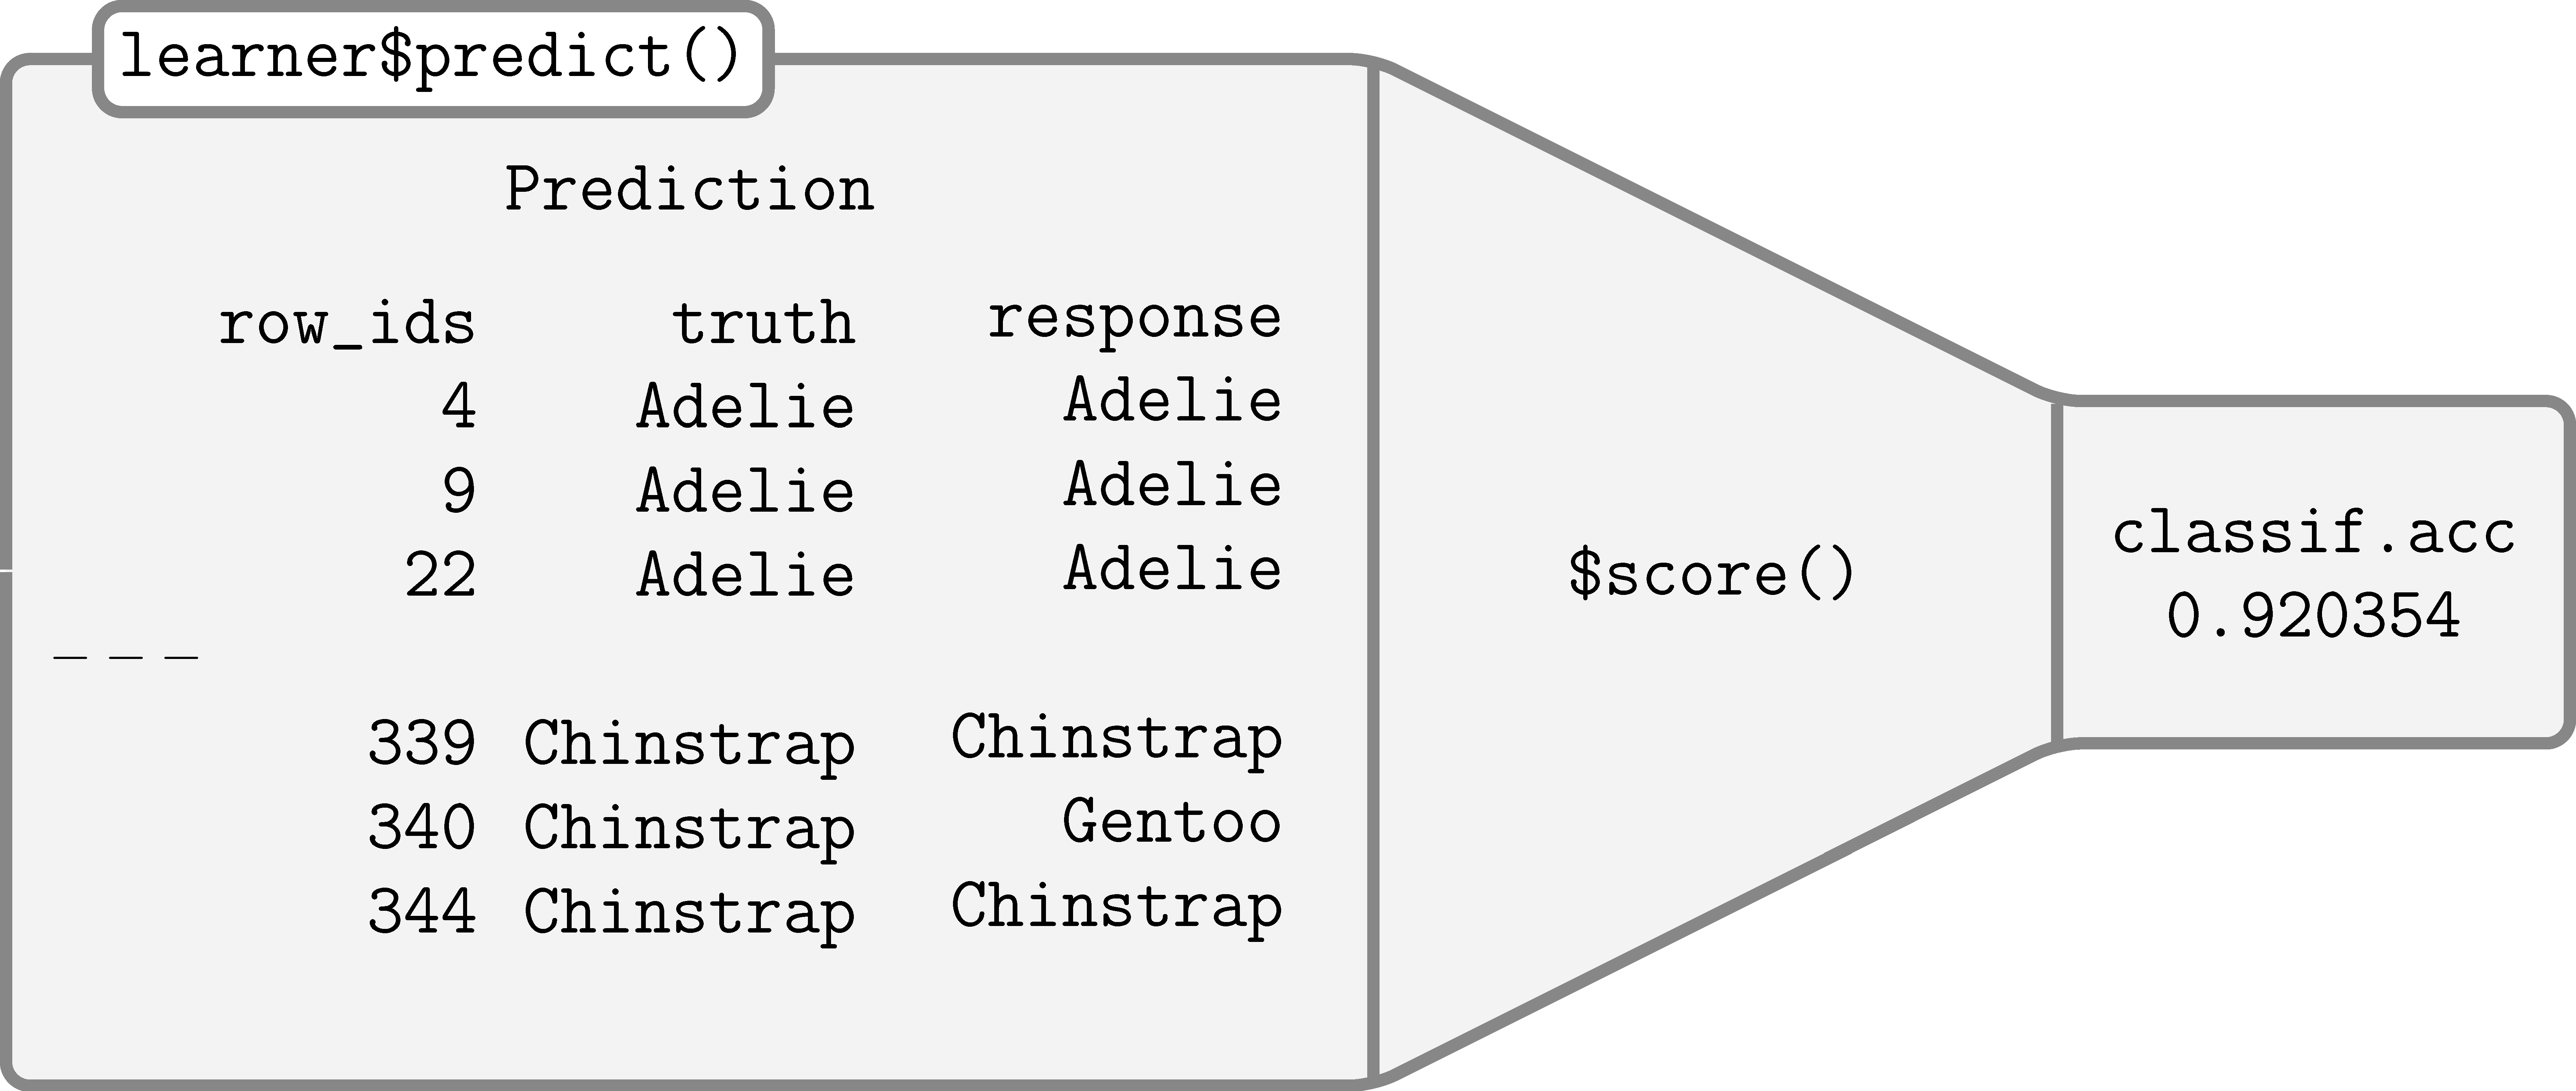
\includegraphics[width=0.8\textwidth,height=\textheight]{chapters/chapter3/Figures/mlr3book_figures-3.png}

}

\caption{\label{fig-score}Illustration of the \texttt{\$score()} method
which aggregates predictions of multiple observations contained in a
prediction object into a single numeric score}

\end{figure}

\hypertarget{sec-resampling}{%
\section{Resampling}\label{sec-resampling}}

Resampling\index{resampling} strategies repeatedly split all available
data into multiple training and test sets, with one repetition
corresponding to what is called a `resampling iteration' in
\href{https://mlr3.mlr-org.com}{\texttt{mlr3}}\index{\texttt{mlr3}}. An
intermediate model is then trained on each training set and the test set
is used to measure the performance in each resampling iteration. The
generalization performance is finally estimated by aggregating the
performance scores over multiple resampling iterations
(Figure~\ref{fig-ml-abstraction}). By repeating the data splitting
process, data points are repeatedly used for both training and testing,
allowing more efficient use of all available data for performance
estimation. Furthermore, a high number of resampling iterations can
reduce the variance in our scores and thus result in a more reliable
performance estimate. This means that the performance estimate is less
likely to be affected by an `unlucky' split (e.g., a split that does not
reflect the original data distribution).

\begin{figure}

{\centering \includegraphics[width=1\textwidth,height=\textheight]{chapters/chapter3/Figures/mlr3book_figures-4.png}

}

\caption{\label{fig-ml-abstraction}A general abstraction of the
performance estimation process. The available data is (repeatedly) split
into training data and test data (data splitting / resampling process).
The learner is trained on each training dataset and produces
intermediate models (learning process). Each intermediate model makes
predictions based on the features in the test data. The performance
measure compares these predictions with the ground truth from the test
data and computes a performance value for each test dataset. All
performance values are aggregated into a scalar value to estimate the
generalization performance (evaluation process).}

\end{figure}

A variety of resampling strategies exist, each with its advantages and
disadvantages, which depend on the number of available samples, the task
complexity, and the type of model.

A very common strategy is k-fold
cross-validation\index{cross-validation}{\marginnote{\begin{footnotesize}Cross-validation\end{footnotesize}}}
(CV), which randomly partitions the data into \(k\) non-overlapping
subsets, called folds (Figure~\ref{fig-cv-illustration}). The \(k\)
models are always trained on \(k-1\) of the folds, with the remaining
fold being used as test data; this process is repeated until each fold
has acted exactly once as test set. Finally, the \(k\) performance
estimates from each fold are aggregated, usually by averaging. CV
guarantees that each observation will be used exactly once in a test
set, making efficient use of the available data for performance
estimation. Common values for \(k\) are 5 and 10, meaning each training
set will consist of 4/5 or 9/10 of the original data, respectively.
Several variations of CV exist, including repeated k-fold
cross-validation\index{cross-validation!repeated k-fold} where the
k-fold process is repeated multiple times, and leave-one-out
cross-validation\index{cross-validation!leave-one-out} (LOO-CV) where
the number of folds is equal to the number of observations, leading to
the test set in each fold consisting of only one observation.

Subsampling\index{subsampling}{\marginnote{\begin{footnotesize}Subsampling\end{footnotesize}}}
and bootstrapping\index{bootstrapping} are two related resampling
strategies. Subsampling randomly selects a given ratio (4/5 and 9/10 are
common) of the data for the training dataset where each observation in
the dataset is drawn \emph{without replacement} from the original
dataset. The model is trained on this data and then tested on the
remaining data, and this process is repeated \(k\) times. This differs
from k-fold CV as the subsets of test data may be overlapping.
Bootstrapping follows the same process as subsampling but data is drawn
\emph{with replacement} from the original dataset. Usually the number of
bootstrap samples equals the size of the original dataset. This means an
observation could be selected multiple times (and thus duplicated) in
the training data (but never more than once per test dataset). On
average, \(1 - e^{-1} \approx 63.2\%\) of the data points will be
contained in the training set during bootstrapping, referred to as
``in-bag'' samples (the other 36.8\% are known as ``out-of-bag''
samples).

Note that terminology regarding resampling strategies is not consistent
across the literature, for example, subsampling is sometimes referred to
as ``repeated holdout'' \index{repeated holdout|see{subsampling}} or
``Monte Carlo
cross-validation''\index{Monte Carlo cross-validation|see{subsampling}}.

The choice of the resampling strategy usually depends on the specific
task at hand and the goals of the performance assessment, but some rules
of thumb are available. If the available data is fairly small
(\(N \leq 500\)), repeated cross-validation with a large number of
repetitions can be used to keep the variance of the performance
estimates low (10 folds and 10 repetitions is a good place to start).
Traditionally, LOO-CV has also been recommended for these small sample
size regimes, but this estimation scheme is quite expensive (except in
special cases where computational shortcuts exist) and
(counterintuitively) suffers from quite high variance. Furthermore,
LOO-CV is also problematic in imbalanced binary classification tasks as
concepts such as stratification (Section~\ref{sec-strat-group}) cannot
be applied. For the \(500 \leq N \leq 50000\) range, 5- to 10-fold CV is
generally recommended. In general, the larger the dataset, the fewer
splits are required, yet sample-size issues can still occur, e.g., due
to imbalanced data. For settings where one is more interested in proper
inference (such as through statistical performance tests or confidence
intervals) than bare point estimators of performance, bootstrapping and
subsampling are often considered, usually with a higher number of
iterations. Bootstrapping has become less common, as having repeated
observations in training data can lead to problems in some machine
learning setups, especially when combined with model selection methods
and nested resampling (as duplicated observations can then end up
simultaneously in training and test sets in nested schemes). Also note
that in all of these common and simple schemes, resampling performance
estimates are not independent, as models are fitted on overlapping
training data, making proper inference less than trivial, but a proper
treatment of these issues is out of scope for us here. For further
details and critical discussion we refer to the literature, e.g.,
Molinaro, Simon, and Pfeiffer (2005), J.-H. Kim (2009), and Bischl et
al. (2012).

\begin{figure}

{\centering 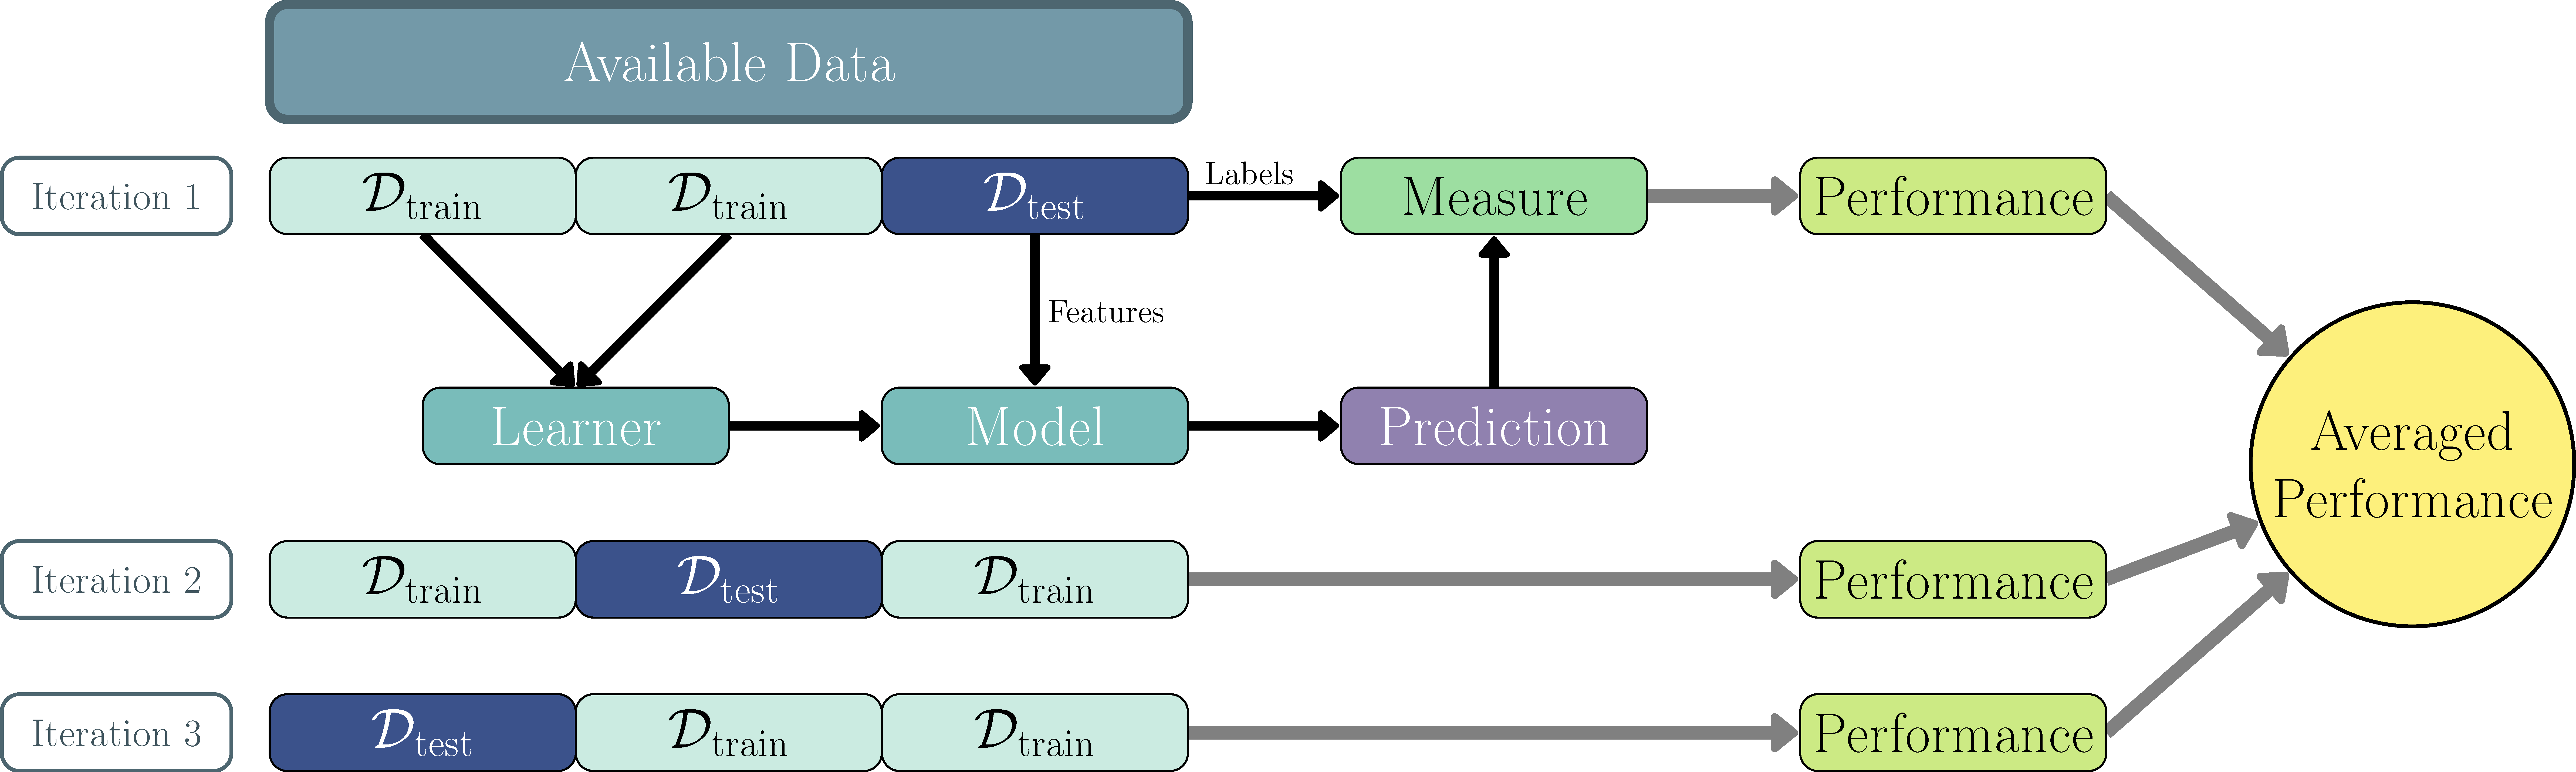
\includegraphics[width=1\textwidth,height=\textheight]{chapters/chapter3/Figures/mlr3book_figures-6.png}

}

\caption{\label{fig-cv-illustration}Illustration of a three-fold
cross-validation.}

\end{figure}

In the rest of this section, we will go through querying and
constructing resampling strategies in \texttt{mlr3}, instantiating
train-test splits, and then performing resampling on learners.

\hypertarget{sec-resampling-construct}{%
\subsection{Constructing a Resampling
Strategy}\label{sec-resampling-construct}}

All implemented resampling strategies are stored in the
\href{https://mlr3.mlr-org.com/reference/mlr_resamplings.html}{\texttt{mlr\_resamplings}}
dictionary.

\begin{Shaded}
\begin{Highlighting}[]
\FunctionTok{as.data.table}\NormalTok{(mlr\_resamplings)}
\end{Highlighting}
\end{Shaded}

\begin{verbatim}
           key                         label        params iters
1:   bootstrap                     Bootstrap ratio,repeats    30
2:      custom                 Custom Splits                  NA
3:   custom_cv Custom Split Cross-Validation                  NA
4:          cv              Cross-Validation         folds    10
5:     holdout                       Holdout         ratio     1
6:    insample           Insample Resampling                   1
7:         loo                 Leave-One-Out                  NA
8: repeated_cv     Repeated Cross-Validation folds,repeats   100
9: subsampling                   Subsampling ratio,repeats    30
\end{verbatim}

The \texttt{params} column shows the parameters of each resampling
strategy (e.g., the train-test splitting \texttt{ratio} or the number of
\texttt{repeats}) and \texttt{iters} displays the number of performed
resampling iterations by default.

\href{https://mlr3.mlr-org.com/reference/Resampling.html}{\texttt{Resampling}}\index{\texttt{Resampling}}{\marginnote{\begin{footnotesize}\texttt{Resampling}\end{footnotesize}}}
objects can be constructed by passing the strategy `key' to the sugar
function
\href{https://mlr3.mlr-org.com/reference/mlr_sugar.html}{\texttt{rsmp()}}\index{\texttt{rsmp()}}{\marginnote{\begin{footnotesize}\texttt{rsmp()}\end{footnotesize}}}.
For example, to construct the holdout strategy with a 4/5 split (2/3 by
default):

\begin{Shaded}
\begin{Highlighting}[]
\FunctionTok{rsmp}\NormalTok{(}\StringTok{"holdout"}\NormalTok{, }\AttributeTok{ratio =} \FloatTok{0.8}\NormalTok{)}
\end{Highlighting}
\end{Shaded}

\begin{verbatim}
<ResamplingHoldout>: Holdout
* Iterations: 1
* Instantiated: FALSE
* Parameters: ratio=0.8
\end{verbatim}

Parameters for objects inheriting from \texttt{Resampling} work in the
same way as measures and learners and can be set, retrieved, and updated
accordingly:

\begin{Shaded}
\begin{Highlighting}[]
\CommentTok{\# three{-}fold CV}
\NormalTok{cv3 }\OtherTok{=} \FunctionTok{rsmp}\NormalTok{(}\StringTok{"cv"}\NormalTok{, }\AttributeTok{folds =} \DecValTok{3}\NormalTok{)}
\CommentTok{\# Subsampling with 3 repeats and 9/10 ratio}
\NormalTok{ss390 }\OtherTok{=} \FunctionTok{rsmp}\NormalTok{(}\StringTok{"subsampling"}\NormalTok{, }\AttributeTok{repeats =} \DecValTok{3}\NormalTok{, }\AttributeTok{ratio =} \FloatTok{0.9}\NormalTok{)}
\CommentTok{\# 2{-}repeats 5{-}fold CV}
\NormalTok{rcv25 }\OtherTok{=} \FunctionTok{rsmp}\NormalTok{(}\StringTok{"repeated\_cv"}\NormalTok{, }\AttributeTok{repeats =} \DecValTok{2}\NormalTok{, }\AttributeTok{folds =} \DecValTok{5}\NormalTok{)}
\end{Highlighting}
\end{Shaded}

When a \texttt{"Resampling"} object is constructed, it is simply a
definition for how the data splitting process will be performed on the
task when running the resampling strategy. However, it is possible to
manually instantiate a resampling strategy, i.e., generate all
train-test splits, by calling the
\texttt{\$instantiate()}\index{\texttt{Resampling}!\texttt{\$instantiate()}}{\marginnote{\begin{footnotesize}\texttt{\$instantiate()}\end{footnotesize}}}
method on a given task. So carrying on our \texttt{tsk("penguins")}
example we can instantiate the three-fold CV object and then view the
row indices of the data selected for training and testing each fold
using \texttt{\$train\_set()} and \texttt{\$test\_set()} respectively:

\begin{Shaded}
\begin{Highlighting}[]
\NormalTok{cv3}\SpecialCharTok{$}\FunctionTok{instantiate}\NormalTok{(tsk\_penguins)}
\CommentTok{\# first 5 observations in first training set}
\NormalTok{cv3}\SpecialCharTok{$}\FunctionTok{train\_set}\NormalTok{(}\DecValTok{1}\NormalTok{)[}\DecValTok{1}\SpecialCharTok{:}\DecValTok{5}\NormalTok{]}
\end{Highlighting}
\end{Shaded}

\begin{verbatim}
[1]  1  9 21 22 23
\end{verbatim}

\begin{Shaded}
\begin{Highlighting}[]
\CommentTok{\# first 5 observations in third test set}
\NormalTok{cv3}\SpecialCharTok{$}\FunctionTok{test\_set}\NormalTok{(}\DecValTok{3}\NormalTok{)[}\DecValTok{1}\SpecialCharTok{:}\DecValTok{5}\NormalTok{]}
\end{Highlighting}
\end{Shaded}

\begin{verbatim}
[1]  2  3  5 10 12
\end{verbatim}

When the aim is to fairly compare multiple learners, best practice
dictates that all learners being compared use the same training data to
build a model and that they use the same test data to evaluate the model
performance. Resampling strategies are instantiated automatically for
you when using the \texttt{resample()} method, which we will discuss
next. Therefore, manually instantiating resampling strategies is rarely
required but might be useful for debugging or digging deeper into a
model's performance.

\hypertarget{sec-resampling-exec}{%
\subsection{Resampling Experiments}\label{sec-resampling-exec}}

The
\href{https://mlr3.mlr-org.com/reference/resample.html}{\texttt{resample()}}\index{\texttt{resample()}}{\marginnote{\begin{footnotesize}\texttt{resample()}\end{footnotesize}}}
function takes a given \texttt{Task}, \texttt{Learner}, and
\href{https://mlr3.mlr-org.com/reference/Resampling.html}{\texttt{Resampling}}
object to run the given resampling strategy. \texttt{resample()}
repeatedly fits a model on training sets, makes predictions on the
corresponding test sets and stores them in a
\href{https://mlr3.mlr-org.com/reference/ResampleResult.html}{\texttt{ResampleResult}}\index{\texttt{ResampleResult}}{\marginnote{\begin{footnotesize}\texttt{ResampleResult}\end{footnotesize}}}
object, which contains all the information needed to estimate the
generalization performance.

\begin{Shaded}
\begin{Highlighting}[]
\NormalTok{rr }\OtherTok{=} \FunctionTok{resample}\NormalTok{(tsk\_penguins, lrn\_rpart, cv3)}
\NormalTok{rr}
\end{Highlighting}
\end{Shaded}

\begin{verbatim}
<ResampleResult> with 3 resampling iterations
  task_id    learner_id resampling_id iteration warnings errors
 penguins classif.rpart            cv         1        0      0
 penguins classif.rpart            cv         2        0      0
 penguins classif.rpart            cv         3        0      0
\end{verbatim}

Each row of the output corresponds to one of the three iterations/folds.
As with \texttt{Prediction} objects, we can calculate the score
\emph{for each iteration} with \texttt{\$score()}:

\begin{Shaded}
\begin{Highlighting}[]
\NormalTok{acc }\OtherTok{=}\NormalTok{ rr}\SpecialCharTok{$}\FunctionTok{score}\NormalTok{(}\FunctionTok{msr}\NormalTok{(}\StringTok{"classif.ce"}\NormalTok{))}
\NormalTok{acc[, .(iteration, classif.ce)]}
\end{Highlighting}
\end{Shaded}

\begin{verbatim}
   iteration classif.ce
1:         1    0.06087
2:         2    0.04348
3:         3    0.06140
\end{verbatim}

\begin{tcolorbox}[enhanced jigsaw, opacitybacktitle=0.6, rightrule=.15mm, opacityback=0, arc=.35mm, breakable, titlerule=0mm, colframe=quarto-callout-tip-color-frame, coltitle=black, bottomrule=.15mm, toprule=.15mm, colback=white, colbacktitle=quarto-callout-tip-color!10!white, bottomtitle=1mm, toptitle=1mm, title=\textcolor{quarto-callout-tip-color}{\faLightbulb}\hspace{0.5em}{Evaluating Train Sets}, leftrule=.75mm, left=2mm]

By default, \texttt{\$score()} evaluates the performance in the
\emph{test} sets in each iteration, however, you could evaluate the
\emph{train} set performance with
\texttt{\$score(predict\_sets\ =\ "train")}.

\end{tcolorbox}

While \texttt{\$score()} returns the performance in each evaluation,
\texttt{\$aggregate()}\index{\texttt{Learner}!\texttt{\$aggregate()}}{\marginnote{\begin{footnotesize}\$aggregate()\end{footnotesize}}},
returns the aggregated score across all resampling iterations.

\begin{Shaded}
\begin{Highlighting}[]
\NormalTok{rr}\SpecialCharTok{$}\FunctionTok{aggregate}\NormalTok{(}\FunctionTok{msr}\NormalTok{(}\StringTok{"classif.ce"}\NormalTok{))}
\end{Highlighting}
\end{Shaded}

\begin{verbatim}
classif.ce 
   0.05525 
\end{verbatim}

By default, the majority of measures will aggregate scores using a macro
average\index{macro average}, which first calculates the measure in each
resampling iteration separately, and then averages these scores across
all iterations. However, it is also possible to aggregate scores using a
micro average\index{micro average}, which pools predictions across
resampling iterations into one
\href{https://mlr3.mlr-org.com/reference/Prediction.html}{\texttt{Prediction}}
object and then computes the measure on this directly:

\begin{Shaded}
\begin{Highlighting}[]
\NormalTok{rr}\SpecialCharTok{$}\FunctionTok{aggregate}\NormalTok{(}\FunctionTok{msr}\NormalTok{(}\StringTok{"classif.ce"}\NormalTok{, }\AttributeTok{average =} \StringTok{"micro"}\NormalTok{))}
\end{Highlighting}
\end{Shaded}

\begin{verbatim}
classif.ce 
   0.05523 
\end{verbatim}

We can see a \emph{small} difference between the two methods.
Classification error is a decomposable loss
(Section~\ref{sec-holdout-scoring}), in fact, if the test sets all had
the same size then the micro and macro methods would be identical (see
box below). For errors like AUC, which are defined across the set of
observations, the difference between micro- and macro-averaging will be
larger. The default type of aggregation method can be found by querying
the \texttt{\$average} field of a
\href{https://mlr3.mlr-org.com/reference/Measure.html}{\texttt{Measure}}
object.

\begin{tcolorbox}[enhanced jigsaw, opacitybacktitle=0.6, rightrule=.15mm, opacityback=0, arc=.35mm, breakable, titlerule=0mm, colframe=quarto-callout-tip-color-frame, coltitle=black, bottomrule=.15mm, toprule=.15mm, colback=white, colbacktitle=quarto-callout-tip-color!10!white, bottomtitle=1mm, toptitle=1mm, title=\textcolor{quarto-callout-tip-color}{\faLightbulb}\hspace{0.5em}{Macro- and Micro-Averaging}, leftrule=.75mm, left=2mm]

As a simple example to explain macro- and micro-averaging, consider the
difference between taking the mean of a vector (micro) compared to the
mean of two group-wise means (macro):

\begin{Shaded}
\begin{Highlighting}[]
\CommentTok{\# macro}
\FunctionTok{mean}\NormalTok{(}\FunctionTok{mean}\NormalTok{(}\FunctionTok{c}\NormalTok{(}\DecValTok{3}\NormalTok{, }\DecValTok{5}\NormalTok{, }\DecValTok{9}\NormalTok{)), }\FunctionTok{mean}\NormalTok{(}\FunctionTok{c}\NormalTok{(}\DecValTok{1}\NormalTok{, }\DecValTok{5}\NormalTok{)))}
\end{Highlighting}
\end{Shaded}

\begin{verbatim}
[1] 5.667
\end{verbatim}

\begin{Shaded}
\begin{Highlighting}[]
\CommentTok{\# micro}
\FunctionTok{mean}\NormalTok{(}\FunctionTok{c}\NormalTok{(}\DecValTok{3}\NormalTok{, }\DecValTok{5}\NormalTok{, }\DecValTok{9}\NormalTok{, }\DecValTok{1}\NormalTok{, }\DecValTok{5}\NormalTok{))}
\end{Highlighting}
\end{Shaded}

\begin{verbatim}
[1] 4.6
\end{verbatim}

In the example shown in the main text where we used
\texttt{tsk("penguins")}, there is a difference in the classification
error between micro and macro methods because the dataset has 344 rows,
which is not divisible by three (the number of folds), hence the test
sets are not of an equal size.

Note that the terms ``macro-averaging'' and ``micro-averaging'' are not
used consistently in the literature, and sometimes refer to different
concepts, e.g., the way in which the performance is aggregated across
classes in a multi-class classification task.

\end{tcolorbox}

The aggregated score returned by \texttt{\$aggregate()} estimates the
generalization performance of our selected learner on the given task
using the resampling strategy defined in the \texttt{Resampling} object.
While we are usually interested in this aggregated score, it can be
useful to look at the individual performance values of each resampling
iteration (as returned by the \texttt{\$score()} method) as well, e.g.,
to see if any of the iterations lead to very different performance
results. Figure~\ref{fig-score-aggregate-resampling} visualizes the
relationship between \texttt{\$score()} and \texttt{\$aggregate()} for a
small example based on the \texttt{"penguins"} task.

\begin{figure}

{\centering \includegraphics[width=1\textwidth,height=\textheight]{chapters/chapter3/Figures/mlr3book_figures-5.png}

}

\caption{\label{fig-score-aggregate-resampling}An example of the
difference between \texttt{\$score()} and \texttt{\$aggregate()}: The
former aggregates predictions to a single score within each resampling
iteration, and the latter aggregates scores across all resampling
iterations.}

\end{figure}

To visualize the resampling results, you can use the
\href{https://mlr3viz.mlr-org.com/reference/autoplot.ResampleResult.html}{\texttt{autoplot.ResampleResult()}}
function to plot scores across folds as boxplots or histograms
(Figure~\ref{fig-resamp-viz}). Histograms can be useful to visually
gauge the variance of the performance results across resampling
iterations, whereas boxplots are often used when multiple learners are
compared side-by-side (see Section~\ref{sec-benchmarking}).

\begin{Shaded}
\begin{Highlighting}[]
\NormalTok{rr }\OtherTok{=} \FunctionTok{resample}\NormalTok{(tsk\_penguins, lrn\_rpart, }\FunctionTok{rsmp}\NormalTok{(}\StringTok{"cv"}\NormalTok{, }\AttributeTok{folds =} \DecValTok{10}\NormalTok{))}
\FunctionTok{autoplot}\NormalTok{(rr, }\AttributeTok{measure =} \FunctionTok{msr}\NormalTok{(}\StringTok{"classif.acc"}\NormalTok{), }\AttributeTok{type =} \StringTok{"boxplot"}\NormalTok{)}
\FunctionTok{autoplot}\NormalTok{(rr, }\AttributeTok{measure =} \FunctionTok{msr}\NormalTok{(}\StringTok{"classif.acc"}\NormalTok{), }\AttributeTok{type =} \StringTok{"histogram"}\NormalTok{)}
\end{Highlighting}
\end{Shaded}

\begin{figure}

\begin{minipage}[t]{0.50\linewidth}

{\centering 

\raisebox{-\height}{

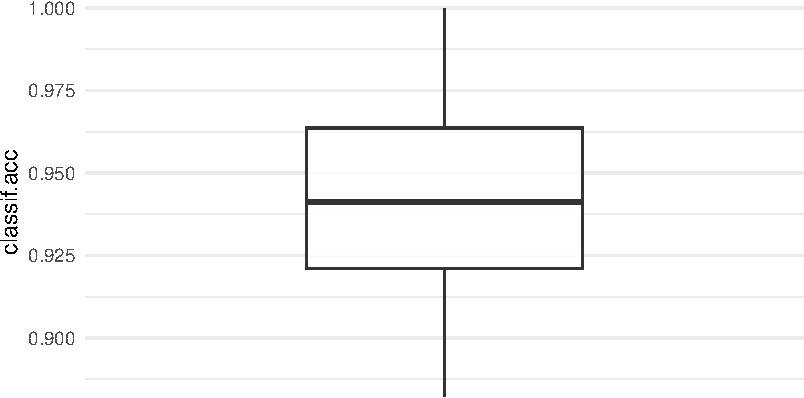
\includegraphics{chapters/chapter3/evaluation_and_benchmarking_files/figure-pdf/fig-resamp-viz-1.pdf}

}

}

\subcaption{\label{fig-resamp-viz-1}Boxplot of accuracy scores.}
\end{minipage}%
%
\begin{minipage}[t]{0.50\linewidth}

{\centering 

\raisebox{-\height}{

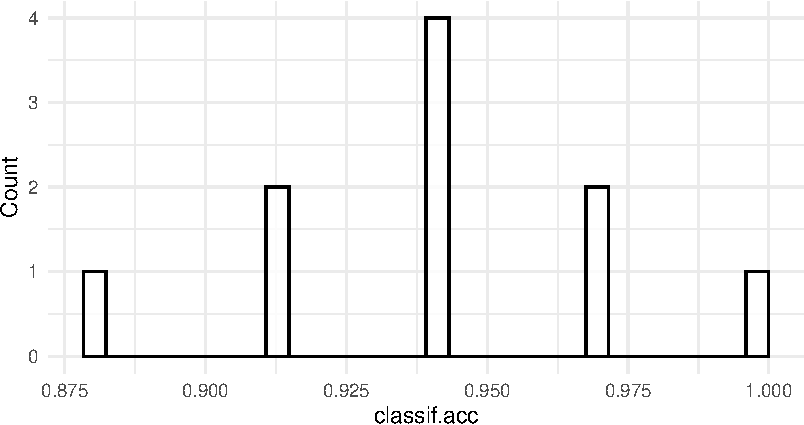
\includegraphics{chapters/chapter3/evaluation_and_benchmarking_files/figure-pdf/fig-resamp-viz-2.pdf}

}

}

\subcaption{\label{fig-resamp-viz-2}Histogram of accuracy scores.}
\end{minipage}%

\caption{\label{fig-resamp-viz}Boxplot and Histogram of accuracy
scores.}

\end{figure}

\hypertarget{sec-resampling-inspect}{%
\subsection{ResampleResult Objects}\label{sec-resampling-inspect}}

As well as being useful for estimating the generalization performance,
the
\href{https://mlr3.mlr-org.com/reference/ResampleResult.html}{\texttt{ResampleResult}}
object can also be used for model inspection. We can use the
\texttt{\$predictions()} method to obtain a list of
\href{https://mlr3.mlr-org.com/reference/Prediction.html}{\texttt{Prediction}}
objects corresponding to the predictions from each resampling iteration.
This can be used to analyze the predictions of individual intermediate
models from each resampling iteration. To understand the class better,
we use it here to manually compute a macro averaged performance
estimate.

\begin{Shaded}
\begin{Highlighting}[]
\CommentTok{\# list of prediction objects}
\NormalTok{rrp }\OtherTok{=}\NormalTok{ rr}\SpecialCharTok{$}\FunctionTok{predictions}\NormalTok{()}
\CommentTok{\# print first two}
\NormalTok{rrp[}\DecValTok{1}\SpecialCharTok{:}\DecValTok{2}\NormalTok{]}
\end{Highlighting}
\end{Shaded}

\begin{verbatim}
[[1]]
<PredictionClassif> for 35 observations:
    row_ids     truth  response
          2    Adelie    Adelie
          4    Adelie    Adelie
         11    Adelie    Adelie
---                            
        333 Chinstrap Chinstrap
        334 Chinstrap Chinstrap
        337 Chinstrap Chinstrap

[[2]]
<PredictionClassif> for 35 observations:
    row_ids     truth response
          1    Adelie   Adelie
         21    Adelie   Adelie
         34    Adelie   Adelie
---                           
        309 Chinstrap   Adelie
        317 Chinstrap   Gentoo
        343 Chinstrap   Gentoo
\end{verbatim}

\begin{Shaded}
\begin{Highlighting}[]
\CommentTok{\# macro averaged performance}
\FunctionTok{mean}\NormalTok{(}\FunctionTok{sapply}\NormalTok{(rrp, }\ControlFlowTok{function}\NormalTok{(.x) .x}\SpecialCharTok{$}\FunctionTok{score}\NormalTok{()))}
\end{Highlighting}
\end{Shaded}

\begin{verbatim}
[1] 0.05807
\end{verbatim}

The \texttt{\$prediction()} method can be used to extract a single
\texttt{Prediction} object that combines the predictions of each
intermediate model across all resampling iterations. The combined
prediction object can, for example, be used to manually compute a
micro-averaged performance estimate (see
Section~\ref{sec-resampling-exec} for how to you can micro-average more
conveniently).

\begin{Shaded}
\begin{Highlighting}[]
\NormalTok{prediction }\OtherTok{=}\NormalTok{ rr}\SpecialCharTok{$}\FunctionTok{prediction}\NormalTok{()}
\NormalTok{prediction}
\end{Highlighting}
\end{Shaded}

\begin{verbatim}
<PredictionClassif> for 344 observations:
    row_ids     truth  response
          2    Adelie    Adelie
          4    Adelie    Adelie
         11    Adelie    Adelie
---                            
        327 Chinstrap Chinstrap
        328 Chinstrap Chinstrap
        341 Chinstrap    Adelie
\end{verbatim}

\begin{Shaded}
\begin{Highlighting}[]
\NormalTok{prediction}\SpecialCharTok{$}\FunctionTok{score}\NormalTok{()}
\end{Highlighting}
\end{Shaded}

\begin{verbatim}
classif.ce 
   0.05814 
\end{verbatim}

By default, the intermediate models produced at each resampling
iteration are discarded after the prediction step to reduce memory
consumption of the \texttt{ResampleResult} object (only the predictions
are required to calculate most performance measures). However, it can
sometimes be useful to inspect, compare, or extract information from
these intermediate models. We can configure the
\href{https://mlr3.mlr-org.com/reference/resample.html}{\texttt{resample()}}
function to keep the fitted intermediate models by setting
\texttt{store\_models\ =\ TRUE}. Each model trained in a specific
resampling iteration can then be accessed via
\texttt{\$learners{[}{[}i{]}{]}\$model}, where \texttt{i} refers to the
\texttt{i}-th resampling iteration:

\begin{Shaded}
\begin{Highlighting}[]
\NormalTok{rr }\OtherTok{=} \FunctionTok{resample}\NormalTok{(tsk\_penguins, lrn\_rpart, cv3, }\AttributeTok{store\_models =} \ConstantTok{TRUE}\NormalTok{)}
\CommentTok{\# get the model from the first iteration}
\NormalTok{rr}\SpecialCharTok{$}\NormalTok{learners[[}\DecValTok{1}\NormalTok{]]}\SpecialCharTok{$}\NormalTok{model}
\end{Highlighting}
\end{Shaded}

\begin{verbatim}
n= 229 

node), split, n, loss, yval, (yprob)
      * denotes terminal node

1) root 229 129 Adelie (0.436681 0.192140 0.371179)  
  2) flipper_length< 207.5 141  42 Adelie (0.702128 0.290780 0.007092)  
    4) bill_length< 44.65 100   3 Adelie (0.970000 0.030000 0.000000) *
    5) bill_length>=44.65 41   3 Chinstrap (0.048780 0.926829 0.024390) *
  3) flipper_length>=207.5 88   4 Gentoo (0.011364 0.034091 0.954545) *
\end{verbatim}

In this example, we could then inspect the most important variables in
each iteration to help us learn more about the respective fitted models:

\begin{Shaded}
\begin{Highlighting}[]
\CommentTok{\# print 2nd and 3rd iteration}
\FunctionTok{lapply}\NormalTok{(rr}\SpecialCharTok{$}\NormalTok{learners[}\DecValTok{2}\SpecialCharTok{:}\DecValTok{3}\NormalTok{], }\ControlFlowTok{function}\NormalTok{(x) x}\SpecialCharTok{$}\NormalTok{model}\SpecialCharTok{$}\NormalTok{variable.importance)}
\end{Highlighting}
\end{Shaded}

\begin{verbatim}
[[1]]
flipper_length    bill_length     bill_depth      body_mass 
         87.23          81.27          66.26          59.46 
        island 
         51.22 

[[2]]
   bill_length flipper_length     bill_depth      body_mass 
         79.06          78.94          59.98          54.35 
        island 
         42.63 
\end{verbatim}

\hypertarget{sec-resamp-custom}{%
\subsection{Custom Resampling}\label{sec-resamp-custom}}

\begin{tcolorbox}[enhanced jigsaw, colframe=quarto-callout-note-color-frame, rightrule=.15mm, bottomrule=.15mm, toprule=.15mm, opacityback=0, colback=white, left=2mm, arc=.35mm, breakable, leftrule=.75mm]
\begin{minipage}[t]{5.5mm}
\textcolor{quarto-callout-note-color}{\faInfo}
\end{minipage}%
\begin{minipage}[t]{\textwidth - 5.5mm}

\textbf{This section covers advanced ML or technical
details.}\vspace{2mm}

\end{minipage}%
\end{tcolorbox}

Sometimes it is necessary to perform resampling with custom splits,
e.g., to reproduce results reported in a study with pre-defined folds.

A custom holdout resampling strategy can be constructed using
\texttt{rsmp("custom")}, where the row IDs of the observations used for
training and testing must be defined manually when instantiated with a
task. In the example below, we first construct a custom holdout
resampling strategy by manually assigning row IDs to the
\texttt{\$train} and \texttt{\$test} fields, then construct a resampling
strategy with two iterations by passing row IDs as list elements:

\begin{Shaded}
\begin{Highlighting}[]
\NormalTok{rsmp\_custom }\OtherTok{=} \FunctionTok{rsmp}\NormalTok{(}\StringTok{"custom"}\NormalTok{)}

\CommentTok{\# resampling strategy with two iterations}
\NormalTok{train\_sets }\OtherTok{=} \FunctionTok{c}\NormalTok{(}\DecValTok{1}\SpecialCharTok{:}\DecValTok{5}\NormalTok{, }\DecValTok{153}\SpecialCharTok{:}\DecValTok{158}\NormalTok{, }\DecValTok{277}\SpecialCharTok{:}\DecValTok{280}\NormalTok{)}
\NormalTok{rsmp\_custom}\SpecialCharTok{$}\FunctionTok{instantiate}\NormalTok{(tsk\_penguins,}
  \AttributeTok{train =} \FunctionTok{list}\NormalTok{(train\_sets, train\_sets }\SpecialCharTok{+} \DecValTok{5}\NormalTok{),}
  \AttributeTok{test =} \FunctionTok{list}\NormalTok{(train\_sets }\SpecialCharTok{+} \DecValTok{15}\NormalTok{, train\_sets }\SpecialCharTok{+} \DecValTok{25}\NormalTok{)}
\NormalTok{)}
\FunctionTok{resample}\NormalTok{(tsk\_penguins, lrn\_rpart, rsmp\_custom)}\SpecialCharTok{$}\FunctionTok{prediction}\NormalTok{()}
\end{Highlighting}
\end{Shaded}

\begin{verbatim}
<PredictionClassif> for 30 observations:
    row_ids     truth response
         16    Adelie   Gentoo
         17    Adelie   Gentoo
         18    Adelie   Gentoo
---                           
        303 Chinstrap   Gentoo
        304 Chinstrap   Gentoo
        305 Chinstrap   Gentoo
\end{verbatim}

A custom cross-validation strategy can be more efficiently constructed
with \texttt{rsmp("custom\_cv")}. In this case, we now have to specify
either a custom \texttt{factor} variable or a \texttt{factor} column
from the data to determine the folds. In the example below, we use a
smaller version of \texttt{tsk("penguins")} and instantiate a custom
two-fold CV strategy using a \texttt{factor} variable called
\texttt{folds} where the first and third rows are used as the test set
in Fold 1, and the second and fourth rows are used as the test set in
Fold 2:

\begin{Shaded}
\begin{Highlighting}[]
\NormalTok{tsk\_small }\OtherTok{=} \FunctionTok{tsk}\NormalTok{(}\StringTok{"penguins"}\NormalTok{)}\SpecialCharTok{$}\FunctionTok{filter}\NormalTok{(}\FunctionTok{c}\NormalTok{(}\DecValTok{1}\NormalTok{, }\DecValTok{100}\NormalTok{, }\DecValTok{200}\NormalTok{, }\DecValTok{300}\NormalTok{))}
\NormalTok{rsmp\_customcv }\OtherTok{=} \FunctionTok{rsmp}\NormalTok{(}\StringTok{"custom\_cv"}\NormalTok{)}
\NormalTok{folds }\OtherTok{=} \FunctionTok{as.factor}\NormalTok{(}\FunctionTok{c}\NormalTok{(}\DecValTok{1}\NormalTok{, }\DecValTok{2}\NormalTok{, }\DecValTok{1}\NormalTok{, }\DecValTok{2}\NormalTok{))}
\NormalTok{rsmp\_customcv}\SpecialCharTok{$}\FunctionTok{instantiate}\NormalTok{(tsk\_small, }\AttributeTok{f =}\NormalTok{ folds)}
\FunctionTok{resample}\NormalTok{(tsk\_small, lrn\_rpart, rsmp\_customcv)}\SpecialCharTok{$}\FunctionTok{predictions}\NormalTok{()}
\end{Highlighting}
\end{Shaded}

\begin{verbatim}
[[1]]
<PredictionClassif> for 2 observations:
 row_ids  truth response
       1 Adelie   Adelie
     200 Gentoo   Adelie

[[2]]
<PredictionClassif> for 2 observations:
 row_ids     truth response
     100    Adelie   Adelie
     300 Chinstrap   Adelie
\end{verbatim}

\hypertarget{sec-strat-group}{%
\subsection{Stratification and Grouping}\label{sec-strat-group}}

\begin{tcolorbox}[enhanced jigsaw, colframe=quarto-callout-note-color-frame, rightrule=.15mm, bottomrule=.15mm, toprule=.15mm, opacityback=0, colback=white, left=2mm, arc=.35mm, breakable, leftrule=.75mm]
\begin{minipage}[t]{5.5mm}
\textcolor{quarto-callout-note-color}{\faInfo}
\end{minipage}%
\begin{minipage}[t]{\textwidth - 5.5mm}

\textbf{This section covers advanced ML or technical
details.}\vspace{2mm}

\end{minipage}%
\end{tcolorbox}

Using column roles (Section~\ref{sec-row-col-roles}), it is possible to
group or stratify observations according to a particular column in the
data. We will look at each of these in turn.

\hypertarget{grouped-resampling}{%
\subsubsection*{\texorpdfstring{Grouped
Resampling\index{grouped resampling}}{Grouped Resampling}}\label{grouped-resampling}}

Keeping observations together when the data is split can be useful, and
sometimes essential, during resampling -- spatial analysis
(Section~\ref{sec-spatiotemporal}) is a prominent example, as
observations belong to natural groups (e.g., countries). When
observations belong to groups, we need to ensure all observations of the
same group belong to \emph{either} the training set \emph{or} the test
set to prevent potential leakage of information between training and
testing. For example, in a longitudinal study, measurements are taken
from the same individual at multiple time points. If we do not group
these, we might overestimate the model's generalization capability to
unseen individuals, because observations of the same individuals might
simultaneously be in the train and test set. In this context, the
leave-one-out cross-validation strategy can be coarsened to the
``leave-one-object-out'' cross-validation strategy, where all
observations associated with a certain group are left out
(Figure~\ref{fig-group}).

\begin{figure}

{\centering 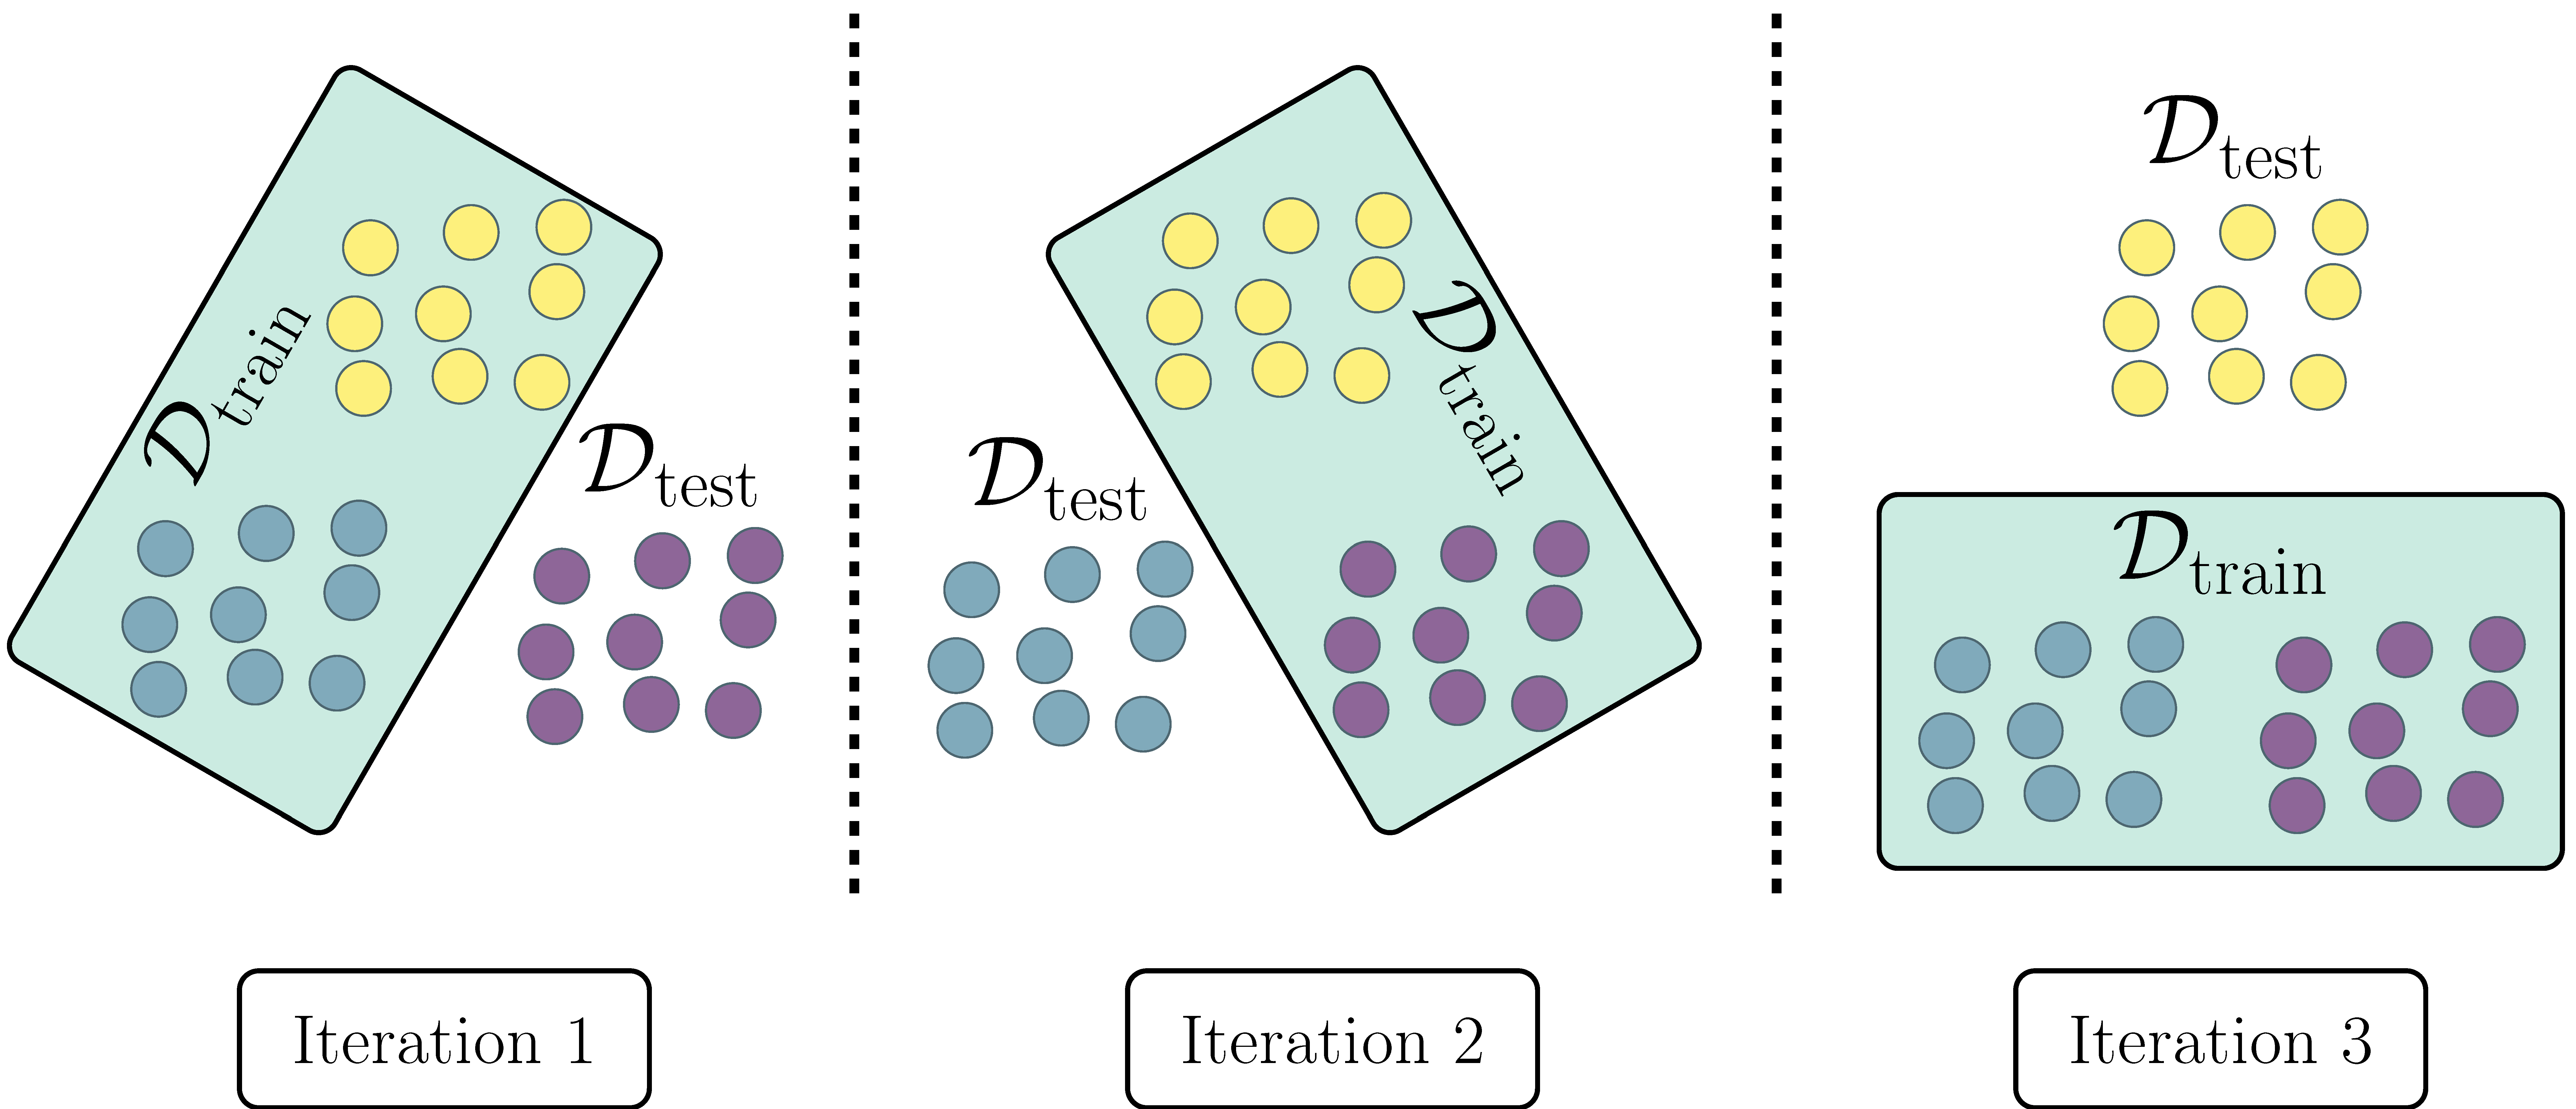
\includegraphics[width=1\textwidth,height=\textheight]{chapters/chapter3/Figures/mlr3book_figures-7.png}

}

\caption{\label{fig-group}Illustration of the train-test splits of a
leave-one-object-out cross-validation with 3 groups of observations
(highlighted by different colors).}

\end{figure}

The \texttt{"group"} column role allows us to specify the column in the
data that defines the group structure of the observations. In the
following code, we construct a leave-one-out resampling strategy, assign
the \texttt{"group"} role to the `year' column of
\texttt{tsk("penguins")}, instantiate the resampling strategy, and
finally show how the years are nicely separated in the first fold.

\begin{Shaded}
\begin{Highlighting}[]
\NormalTok{rsmp\_loo }\OtherTok{=} \FunctionTok{rsmp}\NormalTok{(}\StringTok{"loo"}\NormalTok{)}
\NormalTok{tsk\_grp }\OtherTok{=} \FunctionTok{tsk}\NormalTok{(}\StringTok{"penguins"}\NormalTok{)}
\NormalTok{tsk\_grp}\SpecialCharTok{$}\FunctionTok{set\_col\_roles}\NormalTok{(}\StringTok{"year"}\NormalTok{, }\StringTok{"group"}\NormalTok{)}
\NormalTok{rsmp\_loo}\SpecialCharTok{$}\FunctionTok{instantiate}\NormalTok{(tsk\_grp)}
\FunctionTok{table}\NormalTok{(tsk\_grp}\SpecialCharTok{$}\FunctionTok{data}\NormalTok{(}\AttributeTok{rows =}\NormalTok{ rsmp\_loo}\SpecialCharTok{$}\FunctionTok{train\_set}\NormalTok{(}\DecValTok{1}\NormalTok{), }\AttributeTok{cols =} \StringTok{"year"}\NormalTok{))}
\end{Highlighting}
\end{Shaded}

\begin{verbatim}
year
2008 2009 
 114  120 
\end{verbatim}

\begin{Shaded}
\begin{Highlighting}[]
\FunctionTok{table}\NormalTok{(tsk\_grp}\SpecialCharTok{$}\FunctionTok{data}\NormalTok{(}\AttributeTok{rows =}\NormalTok{ rsmp\_loo}\SpecialCharTok{$}\FunctionTok{test\_set}\NormalTok{(}\DecValTok{1}\NormalTok{), }\AttributeTok{cols =} \StringTok{"year"}\NormalTok{))}
\end{Highlighting}
\end{Shaded}

\begin{verbatim}
year
2007 
 110 
\end{verbatim}

Other cross-validation techniques work in a similar way, where folds are
determined at a group level (as opposed to an observation level).

\hypertarget{stratified-sampling}{%
\subsubsection*{\texorpdfstring{Stratified
Sampling\index{stratified sampling}}{Stratified Sampling}}\label{stratified-sampling}}

Stratified sampling ensures that one or more discrete features within
the training and test sets will have a similar distribution as in the
original task containing all observations. This is especially useful
when a discrete feature is highly imbalanced and we want to make sure
that the distribution of that feature is similar in each resampling
iteration (Figure~\ref{fig-stratification}). We can also stratify on the
target feature to ensure that each intermediate model is fit on training
data where the class distribution of the target is representative of the
actual task, this is useful to ensure target classes are not strongly
under-represented by random chance in individual resampling iterations,
which would lead to degenerate estimations of the generalization
performance.

\begin{figure}

{\centering 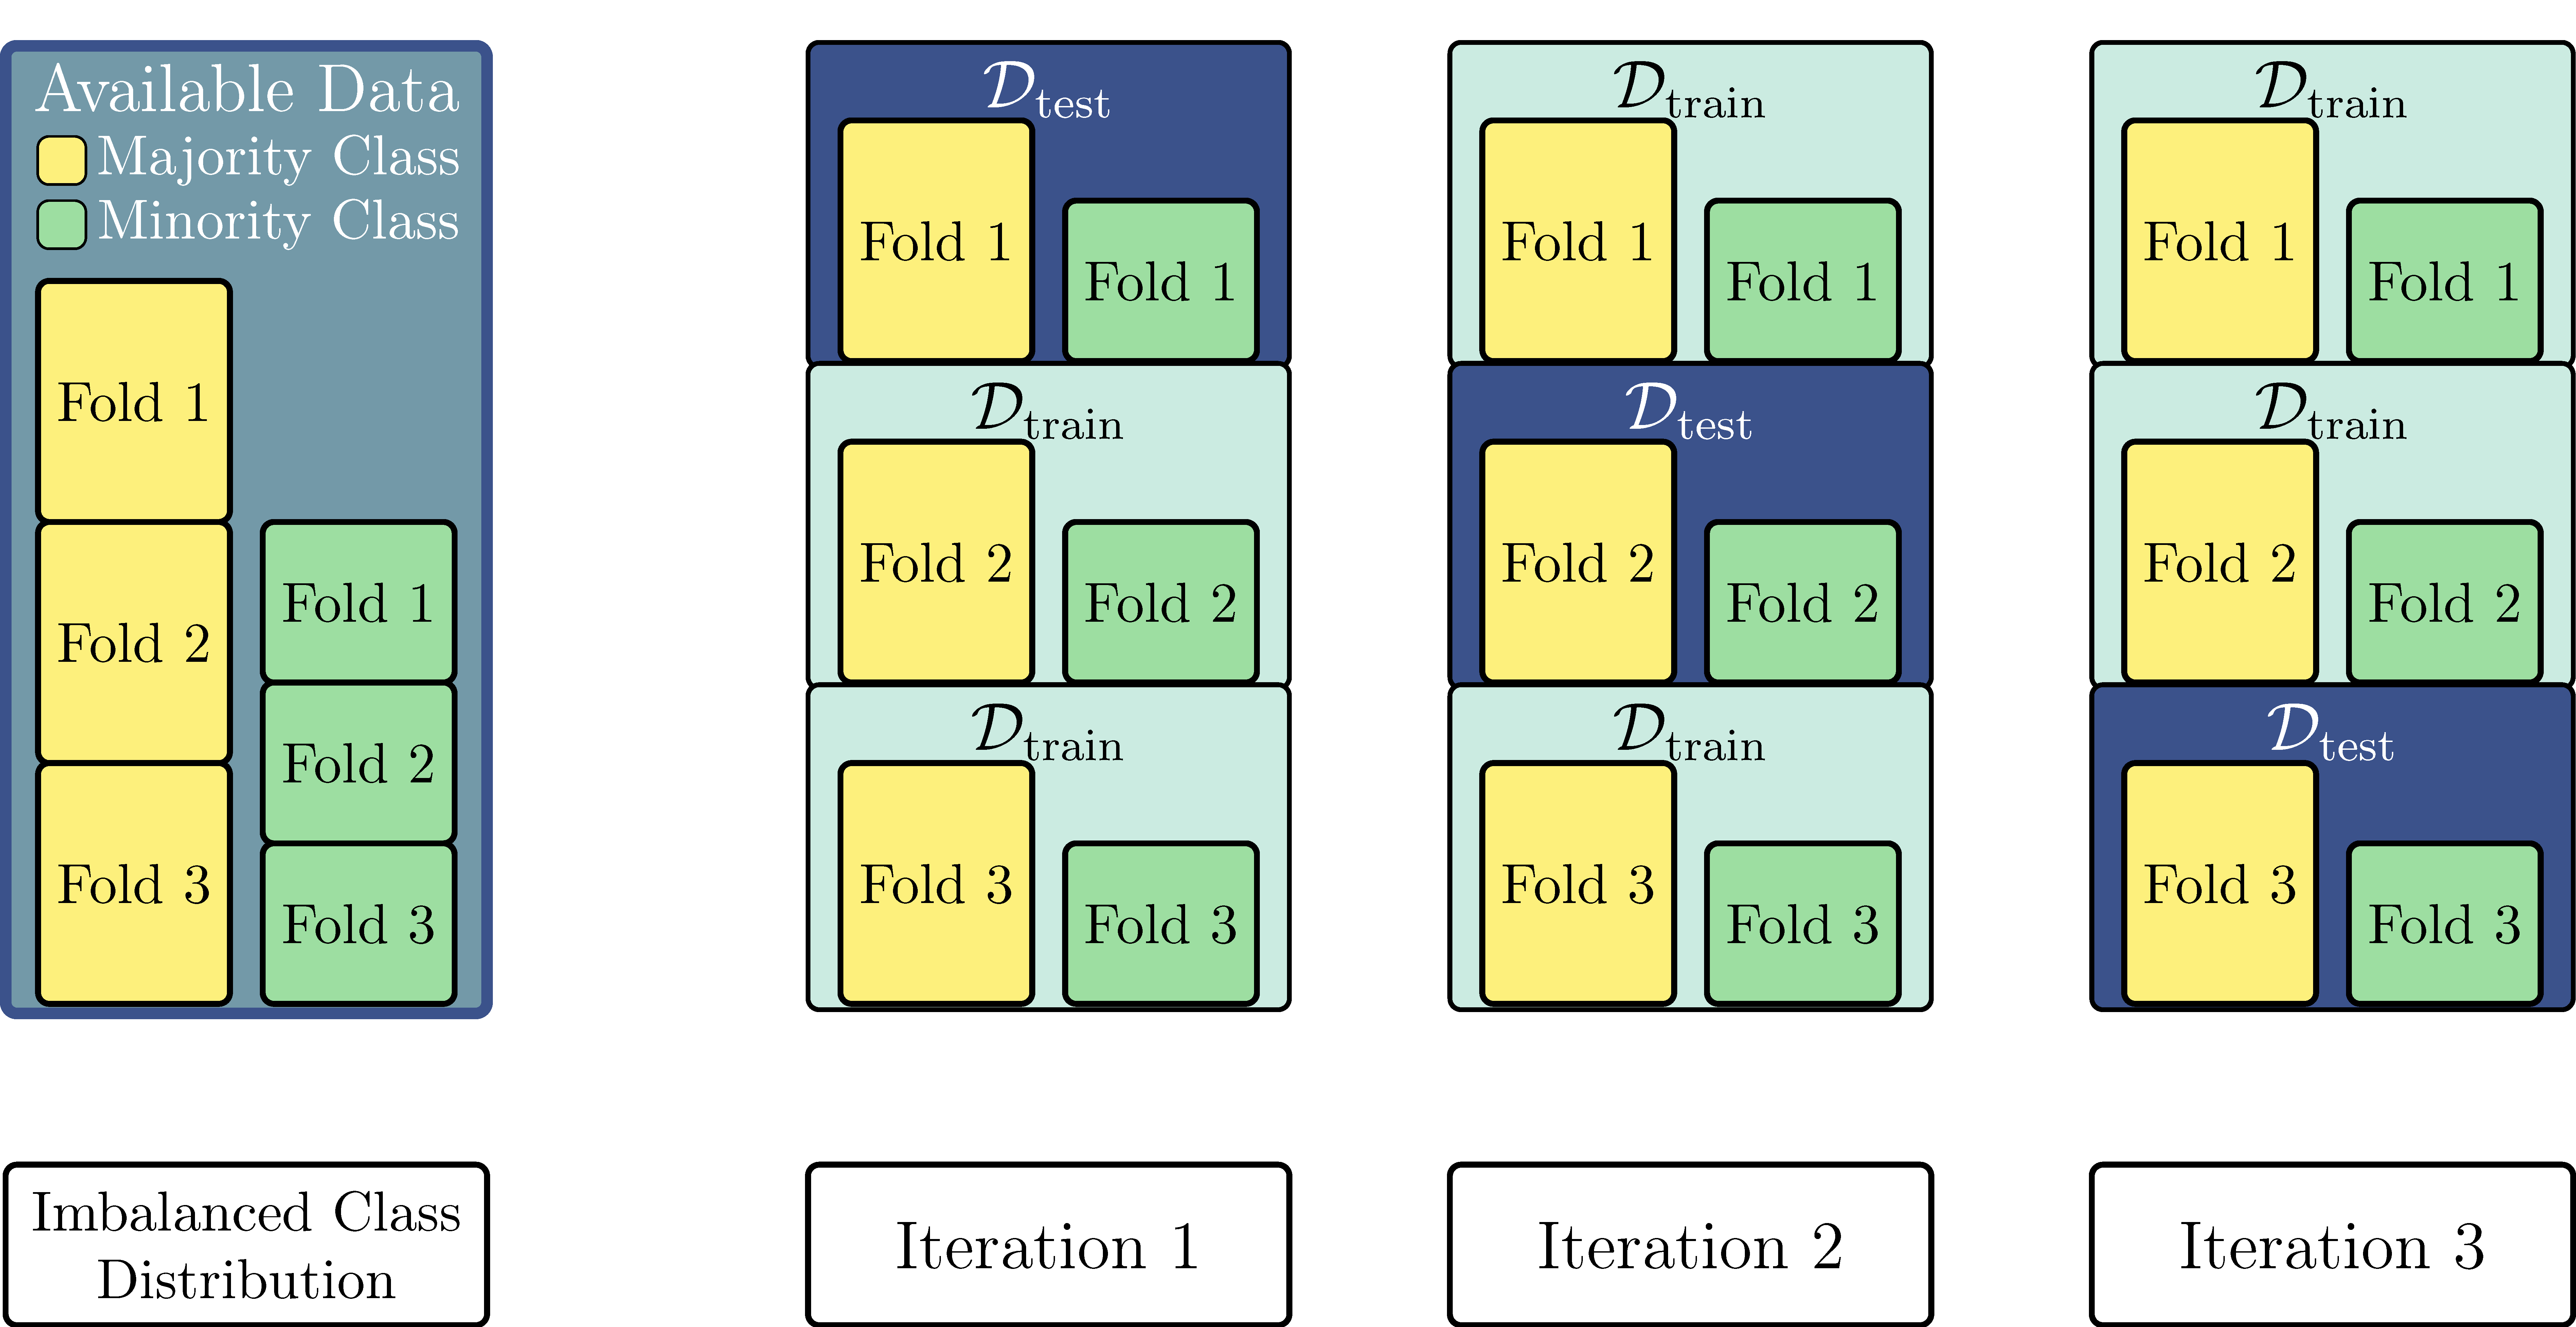
\includegraphics[width=1\textwidth,height=\textheight]{chapters/chapter3/Figures/mlr3book_figures-8.png}

}

\caption{\label{fig-stratification}Illustration of a three-fold
cross-validation with stratification for an imbalanced binary
classification task with a majority class that is about twice as large
as the minority class. In each resampling iteration, the class
distribution from the available data is preserved (which is not
necessarily the case for cross-validation without stratification).}

\end{figure}

Unlike grouping, it is possible to stratify by multiple discrete
features using the \texttt{"stratum"} column role
(Section~\ref{sec-row-col-roles}). In this case, strata would be formed
out of each combination of the stratified features, e.g., for two
stratified features A and B with levels Aa, Ab; Ba, Bb respectively then
the created stratum would have the levels AaBa, AaBb, AbBa, AbBb.

\texttt{tsk("penguins")} displays imbalance in the \texttt{species}
column, as can be seen in the output below:

\begin{Shaded}
\begin{Highlighting}[]
\FunctionTok{prop.table}\NormalTok{(}\FunctionTok{table}\NormalTok{(tsk\_penguins}\SpecialCharTok{$}\FunctionTok{data}\NormalTok{(}\AttributeTok{cols =} \StringTok{"species"}\NormalTok{)))}
\end{Highlighting}
\end{Shaded}

\begin{verbatim}
species
   Adelie Chinstrap    Gentoo 
   0.4419    0.1977    0.3605 
\end{verbatim}

Without specifying a \texttt{"stratum"} column role, the
\texttt{species} column may have quite different class distributions
across the CV folds, as can be seen in the example below.

\begin{Shaded}
\begin{Highlighting}[]
\NormalTok{rsmp\_cv10 }\OtherTok{=} \FunctionTok{rsmp}\NormalTok{(}\StringTok{"cv"}\NormalTok{, }\AttributeTok{folds =} \DecValTok{10}\NormalTok{)}
\NormalTok{rsmp\_cv10}\SpecialCharTok{$}\FunctionTok{instantiate}\NormalTok{(tsk\_penguins)}

\NormalTok{fold1 }\OtherTok{=} \FunctionTok{prop.table}\NormalTok{(}\FunctionTok{table}\NormalTok{(tsk\_penguins}\SpecialCharTok{$}\FunctionTok{data}\NormalTok{(}\AttributeTok{rows =}\NormalTok{ rsmp\_cv10}\SpecialCharTok{$}\FunctionTok{test\_set}\NormalTok{(}\DecValTok{1}\NormalTok{),}
  \AttributeTok{cols =} \StringTok{"species"}\NormalTok{)))}
\NormalTok{fold2 }\OtherTok{=} \FunctionTok{prop.table}\NormalTok{(}\FunctionTok{table}\NormalTok{(tsk\_penguins}\SpecialCharTok{$}\FunctionTok{data}\NormalTok{(}\AttributeTok{rows =}\NormalTok{ rsmp\_cv10}\SpecialCharTok{$}\FunctionTok{test\_set}\NormalTok{(}\DecValTok{2}\NormalTok{),}
  \AttributeTok{cols =} \StringTok{"species"}\NormalTok{)))}

\FunctionTok{rbind}\NormalTok{(}\StringTok{"Fold 1"} \OtherTok{=}\NormalTok{ fold1, }\StringTok{"Fold 2"} \OtherTok{=}\NormalTok{ fold2)}
\end{Highlighting}
\end{Shaded}

\begin{verbatim}
       Adelie Chinstrap Gentoo
Fold 1 0.4286    0.1143 0.4571
Fold 2 0.4286    0.2286 0.3429
\end{verbatim}

We can see across folds how Chinstrap is represented quite differently
(0.11 vs.~0.23)

When imbalance is severe, minority classes might not occur in the
training sets entirely. Consequently, the intermediate models within
these resampling iterations will never predict the missing class,
resulting in a misleading performance estimate for any resampling
strategy without stratification. The code below uses \texttt{species} as
\texttt{"stratum"} column role to illustrate that the distribution of
\texttt{species} in each test set will closely match the original
distribution:

\begin{Shaded}
\begin{Highlighting}[]
\NormalTok{tsk\_str }\OtherTok{=} \FunctionTok{tsk}\NormalTok{(}\StringTok{"penguins"}\NormalTok{)}
\CommentTok{\# set species to have both the \textquotesingle{}target\textquotesingle{} and \textquotesingle{}stratum\textquotesingle{} column role}
\NormalTok{tsk\_str}\SpecialCharTok{$}\FunctionTok{set\_col\_roles}\NormalTok{(}\StringTok{"species"}\NormalTok{, }\FunctionTok{c}\NormalTok{(}\StringTok{"target"}\NormalTok{, }\StringTok{"stratum"}\NormalTok{))}
\NormalTok{rsmp\_cv10}\SpecialCharTok{$}\FunctionTok{instantiate}\NormalTok{(tsk\_str)}

\NormalTok{fold1 }\OtherTok{=} \FunctionTok{prop.table}\NormalTok{(}\FunctionTok{table}\NormalTok{(tsk\_str}\SpecialCharTok{$}\FunctionTok{data}\NormalTok{(}\AttributeTok{rows =}\NormalTok{ rsmp\_cv10}\SpecialCharTok{$}\FunctionTok{test\_set}\NormalTok{(}\DecValTok{1}\NormalTok{),}
  \AttributeTok{cols =} \StringTok{"species"}\NormalTok{)))}
\NormalTok{fold2 }\OtherTok{=} \FunctionTok{prop.table}\NormalTok{(}\FunctionTok{table}\NormalTok{(tsk\_str}\SpecialCharTok{$}\FunctionTok{data}\NormalTok{(}\AttributeTok{rows =}\NormalTok{ rsmp\_cv10}\SpecialCharTok{$}\FunctionTok{test\_set}\NormalTok{(}\DecValTok{2}\NormalTok{),}
  \AttributeTok{cols =} \StringTok{"species"}\NormalTok{)))}

\FunctionTok{rbind}\NormalTok{(}\StringTok{"Fold 1"} \OtherTok{=}\NormalTok{ fold1, }\StringTok{"Fold 2"} \OtherTok{=}\NormalTok{ fold2)}
\end{Highlighting}
\end{Shaded}

\begin{verbatim}
       Adelie Chinstrap Gentoo
Fold 1 0.4444    0.1944 0.3611
Fold 2 0.4444    0.1944 0.3611
\end{verbatim}

You can view the observations that fall into each stratum using the
\texttt{\$strata} field of a \texttt{Task} object, this can be
particularly useful when we are interested in multiple strata:

\begin{Shaded}
\begin{Highlighting}[]
\NormalTok{tsk\_str}\SpecialCharTok{$}\FunctionTok{set\_col\_roles}\NormalTok{(}\StringTok{"year"}\NormalTok{, }\StringTok{"stratum"}\NormalTok{)}
\NormalTok{tsk\_str}\SpecialCharTok{$}\NormalTok{strata}
\end{Highlighting}
\end{Shaded}

\begin{verbatim}
    N                      row_id
1: 50             1,2,3,4,5,6,...
2: 50       51,52,53,54,55,56,...
3: 52 101,102,103,104,105,106,...
4: 34 153,154,155,156,157,158,...
5: 46 187,188,189,190,191,192,...
6: 44 233,234,235,236,237,238,...
7: 26 277,278,279,280,281,282,...
8: 18 303,304,305,306,307,308,...
9: 24 321,322,323,324,325,326,...
\end{verbatim}

\begin{Shaded}
\begin{Highlighting}[]
\CommentTok{\# N above matches with numbers in table below}
\FunctionTok{table}\NormalTok{(tsk\_penguins}\SpecialCharTok{$}\FunctionTok{data}\NormalTok{(}\AttributeTok{cols =} \FunctionTok{c}\NormalTok{(}\StringTok{"species"}\NormalTok{, }\StringTok{"year"}\NormalTok{)))}
\end{Highlighting}
\end{Shaded}

\begin{verbatim}
           year
species     2007 2008 2009
  Adelie      50   50   52
  Chinstrap   26   18   24
  Gentoo      34   46   44
\end{verbatim}

\hypertarget{sec-benchmarking}{%
\section{Benchmarking}\label{sec-benchmarking}}

Benchmarking in supervised machine learning refers to the comparison of
different learners on one or more tasks. When comparing \emph{multiple
learners on a single task} or on a domain consisting of multiple similar
tasks, the main aim is often to rank the learners according to a
pre-defined performance measure and to identify the best-performing
learner for the considered task or domain. When comparing \emph{multiple
learners on multiple tasks}, the main aim is often more of a scientific
nature, e.g., to gain insights into how different learners perform in
different data situations or whether there are certain data properties
that heavily affect the performance of certain learners (or certain
hyperparameters of learners). It is common (and good) practice for
algorithm designers to analyze the generalization performance or runtime
of a newly proposed learning algorithm in comparison to existing
learners in a benchmark experiment\index{benchmark experiment}. Since
benchmarks usually consist of many evaluations that can be run
independently of each other, \texttt{mlr3} offers the possibility of
parallelizing them automatically, which we demonstrate in
Section~\ref{sec-parallel-resample}. In this section, we will focus on
the basic setup of benchmark experiments that will be applicable in the
majority of use cases, in Chapter~\ref{sec-large-benchmarking} we will
look at more complex, large-scale, benchmark experiments.

\hypertarget{sec-bm-design}{%
\subsection{benchmark()}\label{sec-bm-design}}

Benchmark experiments\index{benchmark experiments} in \texttt{mlr3} are
conducted with
\href{https://mlr3.mlr-org.com/reference/benchmark.html}{\texttt{benchmark()}}\index{\texttt{benchmark()}},
which simply runs
\href{https://mlr3.mlr-org.com/reference/resample.html}{\texttt{resample()}}\index{\texttt{resample()}}
on each task and learner separately, then collects the results. The
provided resampling strategy is automatically instantiated on each task
to ensure that all learners are compared against the same training and
test data.

To use the \texttt{benchmark()} function we first call
\href{https://mlr3.mlr-org.com/reference/benchmark_grid.html}{\texttt{benchmark\_grid()}},
which constructs an exhaustive \emph{design} to describe all
combinations of the learners, tasks and resamplings to be used in a
benchmark experiment, and instantiates the resampling strategies. By
example, below we set up a design to see if a random forest, decision
tree, or featureless baseline (Section~\ref{sec-basics-featureless}),
performs best across two classification tasks.

\begin{Shaded}
\begin{Highlighting}[]
\NormalTok{tasks }\OtherTok{=} \FunctionTok{tsks}\NormalTok{(}\FunctionTok{c}\NormalTok{(}\StringTok{"german\_credit"}\NormalTok{, }\StringTok{"sonar"}\NormalTok{))}
\NormalTok{learners }\OtherTok{=} \FunctionTok{lrns}\NormalTok{(}\FunctionTok{c}\NormalTok{(}\StringTok{"classif.rpart"}\NormalTok{, }\StringTok{"classif.ranger"}\NormalTok{,}
  \StringTok{"classif.featureless"}\NormalTok{), }\AttributeTok{predict\_type =} \StringTok{"prob"}\NormalTok{)}
\NormalTok{rsmp\_cv5 }\OtherTok{=} \FunctionTok{rsmp}\NormalTok{(}\StringTok{"cv"}\NormalTok{, }\AttributeTok{folds =} \DecValTok{5}\NormalTok{)}

\NormalTok{design }\OtherTok{=} \FunctionTok{benchmark\_grid}\NormalTok{(tasks, learners, rsmp\_cv5)}
\FunctionTok{head}\NormalTok{(design)}
\end{Highlighting}
\end{Shaded}

\begin{verbatim}
            task             learner resampling
1: german_credit       classif.rpart         cv
2: german_credit      classif.ranger         cv
3: german_credit classif.featureless         cv
4:         sonar       classif.rpart         cv
5:         sonar      classif.ranger         cv
6:         sonar classif.featureless         cv
\end{verbatim}

The resulting design is essentially just a \texttt{data.table}, which
can be modified if you want to remove particular combinations or could
even be created from scratch without the \texttt{benchmark\_grid()}
function. Note that this \texttt{data.table} has list columns that
contain R6 objects of tasks, learners, and resampling instances.

\begin{tcolorbox}[enhanced jigsaw, opacitybacktitle=0.6, rightrule=.15mm, opacityback=0, arc=.35mm, breakable, titlerule=0mm, colframe=quarto-callout-warning-color-frame, coltitle=black, bottomrule=.15mm, toprule=.15mm, colback=white, colbacktitle=quarto-callout-warning-color!10!white, bottomtitle=1mm, toptitle=1mm, title=\textcolor{quarto-callout-warning-color}{\faExclamationTriangle}\hspace{0.5em}{Reproducibility When Using \texttt{benchmark\_grid()}}, leftrule=.75mm, left=2mm]

By default,
\href{https://mlr3.mlr-org.com/reference/benchmark_grid.html}{\texttt{benchmark\_grid()}}
instantiates the resamplings on the tasks, which means that concrete
train-test splits are generated. Since this process is stochastic, it is
necessary to set a seed \textbf{before} calling
\texttt{benchmark\_grid()} to ensure reproducibility of the data splits.

\end{tcolorbox}

The constructed benchmark design can then be passed to
\texttt{benchmark()} to run the experiment and the result is a
\href{https://mlr3.mlr-org.com/reference/BenchmarkResult.html}{\texttt{BenchmarkResult}}
object:

\begin{Shaded}
\begin{Highlighting}[]
\NormalTok{bmr }\OtherTok{=} \FunctionTok{benchmark}\NormalTok{(design)}
\NormalTok{bmr}
\end{Highlighting}
\end{Shaded}

\begin{verbatim}
<BenchmarkResult> of 30 rows with 6 resampling runs
 nr       task_id          learner_id resampling_id iters warnings
  1 german_credit       classif.rpart            cv     5        0
  2 german_credit      classif.ranger            cv     5        0
  3 german_credit classif.featureless            cv     5        0
  4         sonar       classif.rpart            cv     5        0
  5         sonar      classif.ranger            cv     5        0
  6         sonar classif.featureless            cv     5        0
1 variable not shown: [errors]
\end{verbatim}

As \texttt{benchmark()} is just an extension of \texttt{resample()}, we
can once again use \texttt{\$score()}, or \texttt{\$aggregate()}
depending on your use-case, though note that in this case
\texttt{\$score()} will return results over each fold of each
learner/task/resampling combination.

\begin{Shaded}
\begin{Highlighting}[]
\NormalTok{bmr}\SpecialCharTok{$}\FunctionTok{score}\NormalTok{()[}\FunctionTok{c}\NormalTok{(}\DecValTok{1}\NormalTok{, }\DecValTok{7}\NormalTok{, }\DecValTok{13}\NormalTok{), .(iteration, task\_id, learner\_id, classif.ce)]}
\end{Highlighting}
\end{Shaded}

\begin{verbatim}
   iteration       task_id          learner_id classif.ce
1:         1 german_credit       classif.rpart      0.280
2:         2 german_credit      classif.ranger      0.235
3:         3 german_credit classif.featureless      0.275
\end{verbatim}

\begin{Shaded}
\begin{Highlighting}[]
\NormalTok{bmr}\SpecialCharTok{$}\FunctionTok{aggregate}\NormalTok{()[, .(task\_id, learner\_id, classif.ce)]}
\end{Highlighting}
\end{Shaded}

\begin{verbatim}
         task_id          learner_id classif.ce
1: german_credit       classif.rpart     0.2760
2: german_credit      classif.ranger     0.2490
3: german_credit classif.featureless     0.3000
4:         sonar       classif.rpart     0.2840
5:         sonar      classif.ranger     0.1535
6:         sonar classif.featureless     0.4661
\end{verbatim}

This would conclude a basic benchmark experiment where you can draw
tentative conclusions about model performance, in this case we would
possibly conclude that the random forest is the best of all three models
on each task. We draw conclusions cautiously here as we have not run any
statistical tests or included standard errors of measures, so we cannot
definitively say if one model outperforms the other.

As the results of \texttt{\$score()} and \texttt{\$aggregate()} are
returned in a \texttt{data.table}, you can post-process and analyze the
results in any way you want. A common \emph{mistake} is to average the
learner performance across all tasks when the tasks vary significantly.
This is a mistake as averaging the performance will miss out important
insights into how learners compare on `easier' or more `difficult'
predictive problems. A more robust alternative to compare the overall
algorithm performance across multiple tasks is to compute the ranks of
each learner on each task separately and then calculate the average
ranks. This can provide a better comparison as task-specific `quirks'
are taken into account by comparing learners within tasks before
comparing them across tasks. However, using ranks will lose information
about the numerical differences between the calculated performance
scores. Analysis of benchmark experiments, including statistical tests,
is covered in more detail in Section~\ref{sec-benchmark-analysis}.

\hypertarget{sec-bm-resamp}{%
\subsection{BenchmarkResult Objects}\label{sec-bm-resamp}}

A
\href{https://mlr3.mlr-org.com/reference/BenchmarkResult.html}{\texttt{BenchmarkResult}}
object is a collection of multiple
\href{https://mlr3.mlr-org.com/reference/ResampleResult.html}{\texttt{ResampleResult}}\index{\texttt{ResampleResult}}
objects.

\begin{Shaded}
\begin{Highlighting}[]
\NormalTok{bmrdt }\OtherTok{=} \FunctionTok{as.data.table}\NormalTok{(bmr)}
\NormalTok{bmrdt[}\DecValTok{1}\SpecialCharTok{:}\DecValTok{2}\NormalTok{, .(task, learner, resampling, iteration)]}
\end{Highlighting}
\end{Shaded}

\begin{verbatim}
                task                   learner         resampling
1: <TaskClassif[51]> <LearnerClassifRpart[38]> <ResamplingCV[20]>
2: <TaskClassif[51]> <LearnerClassifRpart[38]> <ResamplingCV[20]>
1 variable not shown: [iteration]
\end{verbatim}

The contents of a \texttt{BenchmarkResult} and \texttt{ResampleResult}
(Section~\ref{sec-resampling-inspect}) are almost identical and the
stored \texttt{ResampleResult}s can be extracted via the
\texttt{\$resample\_result(i)} method, where \texttt{i} is the index of
the performed resample experiment. This allows us to investigate the
extracted \texttt{ResampleResult} and individual resampling iterations
as shown in Section~\ref{sec-resampling}, as well as the predictions
from each fold with \texttt{\$resample\_result(i)\$predictions()}.

\begin{Shaded}
\begin{Highlighting}[]
\NormalTok{rr1 }\OtherTok{=}\NormalTok{ bmr}\SpecialCharTok{$}\FunctionTok{resample\_result}\NormalTok{(}\DecValTok{1}\NormalTok{)}
\NormalTok{rr1}
\end{Highlighting}
\end{Shaded}

\begin{verbatim}
<ResampleResult> with 5 resampling iterations
       task_id    learner_id resampling_id iteration warnings errors
 german_credit classif.rpart            cv         1        0      0
 german_credit classif.rpart            cv         2        0      0
 german_credit classif.rpart            cv         3        0      0
 german_credit classif.rpart            cv         4        0      0
 german_credit classif.rpart            cv         5        0      0
\end{verbatim}

\begin{Shaded}
\begin{Highlighting}[]
\NormalTok{rr2 }\OtherTok{=}\NormalTok{ bmr}\SpecialCharTok{$}\FunctionTok{resample\_result}\NormalTok{(}\DecValTok{2}\NormalTok{)}
\end{Highlighting}
\end{Shaded}

In addition,
\href{https://mlr3.mlr-org.com/reference/as_benchmark_result.html}{\texttt{as\_benchmark\_result()}}
can be used to convert objects from \texttt{ResampleResult} to
\texttt{BenchmarkResult}. The \texttt{c()}-method can be used to combine
multiple \texttt{BenchmarkResult} objects, which can be useful when
conducting experiments across multiple machines:

\begin{Shaded}
\begin{Highlighting}[]
\NormalTok{bmr1 }\OtherTok{=} \FunctionTok{as\_benchmark\_result}\NormalTok{(rr1)}
\NormalTok{bmr2 }\OtherTok{=} \FunctionTok{as\_benchmark\_result}\NormalTok{(rr2)}

\FunctionTok{c}\NormalTok{(bmr1, bmr2)}
\end{Highlighting}
\end{Shaded}

\begin{verbatim}
<BenchmarkResult> of 10 rows with 2 resampling runs
 nr       task_id     learner_id resampling_id iters warnings errors
  1 german_credit  classif.rpart            cv     5        0      0
  2 german_credit classif.ranger            cv     5        0      0
\end{verbatim}

Boxplots are most commonly used to visualize benchmark experiments as
they can intuitively summarize results across tasks and learners
simultaneously.

\begin{Shaded}
\begin{Highlighting}[]
\FunctionTok{autoplot}\NormalTok{(bmr, }\AttributeTok{measure =} \FunctionTok{msr}\NormalTok{(}\StringTok{"classif.acc"}\NormalTok{))}
\end{Highlighting}
\end{Shaded}

\begin{figure}

{\centering 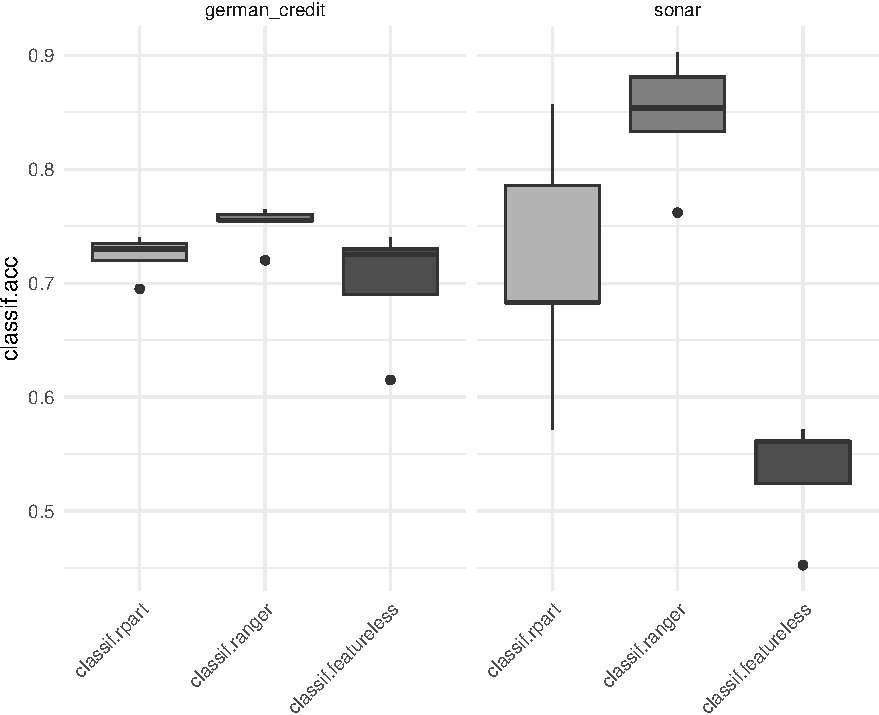
\includegraphics[width=0.7\textwidth,height=\textheight]{chapters/chapter3/evaluation_and_benchmarking_files/figure-pdf/fig-benchmark-box-1.pdf}

}

\caption{\label{fig-benchmark-box}Boxplots of accuracy scores for each
learner across resampling iterations and the three tasks. Random forests
(\texttt{lrn("classif.ranger")}) consistently outperforms the other
learners.}

\end{figure}

\hypertarget{sec-roc}{%
\section{Evaluation of Binary Classifiers}\label{sec-roc}}

In Section~\ref{sec-basics-classif-learner} we touched on the concept of
a confusion matrix and how it can be used to break down classification
errors in more detail. In this section, we will look at specialized
performance measures for binary
classification\index{classification!binary} in more detail. We will
first return to the confusion matrix and discuss measures that can be
derived from it and then will look at ROC\index{ROC} analysis which
builds on these measures. See Chapters 7 and 8 of Provost and Fawcett
(2013) for a more detailed introduction to ROC measures.

\hypertarget{confusion-matrix-1}{%
\subsection{Confusion Matrix}\label{confusion-matrix-1}}

To recap, a confusion matrix\index{confusion matrix} summarizes the
following quantities in a two-dimensional contingency table (see also
Figure~\ref{fig-confusion}):

\begin{itemize}
\tightlist
\item
  True positives\index{true positives} (TPs): Positive instances that
  are correctly classified as positive.
\item
  True negatives\index{true negatives} (TNs): Negative instances that
  are correctly classified as negative.
\item
  False positives\index{false positives} (FPs): Negative instances that
  are incorrectly classified as positive.
\item
  False negatives\index{false negatives} (FNs): Positive instances that
  are incorrectly classified as negative.
\end{itemize}

Different applications may have a particular interest in one (or
multiple) of the aforementioned quantities. For example, the
\texttt{tsk("spam")} classification task is concerned with classifying
if mail is spam (positive class) or not (negative class). In this case,
we are likely to accept FNs (some spam classified as genuine mail) as
long as we have a low number of FPs (genuine and possibly important mail
classified as spam). In another example, say we are predicting if a
travel bag contains a weapon (positive class) or not (negative class) at
an airport. This classifier must have a very high number of TPs (as FNs
are not acceptable at all), even if this comes at the expense of more
FPs (false alarms).

As we saw in Section~\ref{sec-basics-classif-learner}, it is possible
for a classifier to have a good classification accuracy but to overlook
the nuances provided by a full confusion matrix, as in the following
\texttt{tsk("german\_credit")} example:

\begin{Shaded}
\begin{Highlighting}[]
\NormalTok{tsk\_german }\OtherTok{=} \FunctionTok{tsk}\NormalTok{(}\StringTok{"german\_credit"}\NormalTok{)}
\NormalTok{lrn\_ranger }\OtherTok{=} \FunctionTok{lrn}\NormalTok{(}\StringTok{"classif.ranger"}\NormalTok{, }\AttributeTok{predict\_type =} \StringTok{"prob"}\NormalTok{)}
\NormalTok{splits }\OtherTok{=} \FunctionTok{partition}\NormalTok{(tsk\_german, }\AttributeTok{ratio =} \FloatTok{0.8}\NormalTok{)}

\NormalTok{lrn\_ranger}\SpecialCharTok{$}\FunctionTok{train}\NormalTok{(tsk\_german, splits}\SpecialCharTok{$}\NormalTok{train)}
\NormalTok{prediction }\OtherTok{=}\NormalTok{ lrn\_ranger}\SpecialCharTok{$}\FunctionTok{predict}\NormalTok{(tsk\_german, splits}\SpecialCharTok{$}\NormalTok{test)}
\NormalTok{prediction}\SpecialCharTok{$}\FunctionTok{score}\NormalTok{(}\FunctionTok{msr}\NormalTok{(}\StringTok{"classif.acc"}\NormalTok{))}
\end{Highlighting}
\end{Shaded}

\begin{verbatim}
classif.acc 
       0.72 
\end{verbatim}

\begin{Shaded}
\begin{Highlighting}[]
\NormalTok{prediction}\SpecialCharTok{$}\NormalTok{confusion}
\end{Highlighting}
\end{Shaded}

\begin{verbatim}
        truth
response good bad
    good  123  39
    bad    17  21
\end{verbatim}

The classification accuracy only takes into account the TPs and TNs,
whereas the confusion matrix provides a more holistic picture of the
classifier's performance.

On their own, the absolute numbers in a confusion matrix can be less
useful when there is class imbalance. Instead, several normalized
measures can be derived (Figure~\ref{fig-confusion}):

\begin{itemize}
\tightlist
\item
  \textbf{True Positive
  Rate\index{true positive rate}\index{sensitivity|see{measures, true positive rate}}\index{recall|see{measures, true positive rate}}
  (TPR)}, \textbf{Sensitivity} or \textbf{Recall}: How many of the true
  positives did we predict as positive?
\item
  \textbf{True Negative
  Rate\index{true negative rate}\index{specificity|see{measures, true negative rate}}
  (TNR)} or \textbf{Specificity}: How many of the true negatives did we
  predict as negative?
\item
  \textbf{False Positive Rate\index{false positive rate} (FPR)}, or
  \(1 -\) \textbf{Specificity}: How many of the true negatives did we
  predict as positive?
\item
  \textbf{Positive Predictive
  Value\index{positive predictive value}\index{precision|see{measures, positive predictive value}}
  (PPV)} or \textbf{Precision}: If we predict positive how likely is it
  a true positive?
\item
  \textbf{Negative Predictive Value\index{negative predictive value}
  (NPV)}: If we predict negative how likely is it a true negative?
\item
  \textbf{Accuracy (ACC)\index{accuracy}}: The proportion of correctly
  classified instances out of the total number of instances.
\item
  \textbf{F1-score\index{F1}}: The harmonic mean of precision and
  recall, which balances the trade-off between precision and recall. It
  is calculated as
  \(2 \times \frac{Precision \times Recall}{Precision + Recall}\).
\end{itemize}

\begin{figure}

{\centering 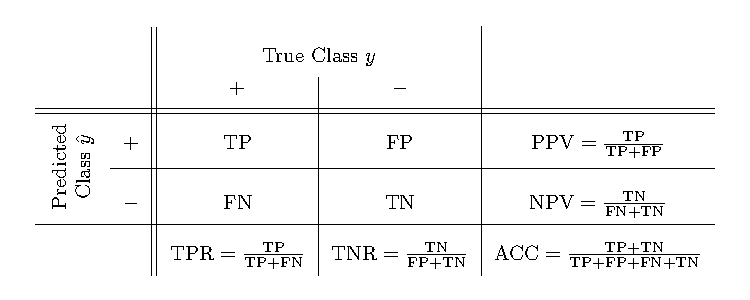
\includegraphics[width=1\textwidth,height=\textheight]{chapters/chapter3/Figures/confusion_matrix.pdf}

}

\caption{\label{fig-confusion}Binary confusion matrix of ground truth
class vs.~predicted class.}

\end{figure}

The
\href{https://cran.r-project.org/package=mlr3measures}{\texttt{mlr3measures}}
package allows you to compute several common confusion matrix-based
measures using the
\href{https://www.rdocumentation.org/packages/mlr3measures/topics/confusion_matrix}{\texttt{confusion\_matrix()}}
function:

\begin{Shaded}
\begin{Highlighting}[]
\NormalTok{mlr3measures}\SpecialCharTok{::}\FunctionTok{confusion\_matrix}\NormalTok{(}\AttributeTok{truth =}\NormalTok{ prediction}\SpecialCharTok{$}\NormalTok{truth,}
  \AttributeTok{response =}\NormalTok{ prediction}\SpecialCharTok{$}\NormalTok{response, }\AttributeTok{positive =}\NormalTok{ tsk\_german}\SpecialCharTok{$}\NormalTok{positive)}
\end{Highlighting}
\end{Shaded}

\begin{verbatim}
        truth
response good bad
    good  123  39
    bad    17  21
acc :  0.7200; ce  :  0.2800; dor :  3.8959; f1  :  0.8146 
fdr :  0.2407; fnr :  0.1214; fomr:  0.4474; fpr :  0.6500 
mcc :  0.2670; npv :  0.5526; ppv :  0.7593; tnr :  0.3500 
tpr :  0.8786 
\end{verbatim}

We now have a better idea of the random forest predictions on
\texttt{tsk("german\_credit")}, in particular, the false positive rate
is quite high. It is generally difficult to achieve a high TPR and low
FPR simultaneously because there is often a trade-off between the two
rates. When a binary classifier predicts probabilities instead of
discrete classes (\texttt{predict\_type\ =\ "prob"}), we could set a
threshold to cut off the probabilities to change how we assign
observations to the positive/negative class (see
Section~\ref{sec-classif-prediction}). Increasing the threshold for
identifying the positive cases, leads to a higher number of negative
predictions, fewer positive predictions, and therefore a lower (and
better) FPR but a lower (and worse) TPR -- the reverse holds if we lower
the threshold. Instead of arbitrarily changing a threshold to `game'
these two numbers, a more robust way to tradeoff between TPR and FPR is
to use ROC analysis, discussed next.

\hypertarget{sec-roc-space}{%
\subsection{ROC Analysis}\label{sec-roc-space}}

ROC\index{ROC} (Receiver Operating Characteristic) analysis is widely
used to evaluate binary classifiers by visualizing the trade-off between
the TPR and the FPR.

The ROC curve is a line graph with TPR on the y-axis and the FPR on the
x-axis. To understand the usefulness of this curve, first consider the
simple case of a hard labeling classifier
(\texttt{predict\_type\ =\ "response"}) that classifies observations as
either positive or negative. This classifier would be represented as a
single point in the ROC space (see Figure~\ref{fig-roc}, panel (a)). The
best classifier would lie on the top-left corner where the TPR is \(1\)
and the FPR is \(0\). Classifiers on the diagonal predict class labels
randomly (with different class proportions). For example, if each
positive instance will be randomly classified (ignoring features) with
25\% as the positive class, we would obtain a TPR of 0.25. If we assign
each negative instance randomly to the positive class, we would have an
FPR of 0.25. In practice, we should never obtain a classifier below the
diagonal and a point in the ROC space below the diagonal might indicate
that the positive and negative class labels have been switched by the
classifier.

\begin{figure}

{\centering 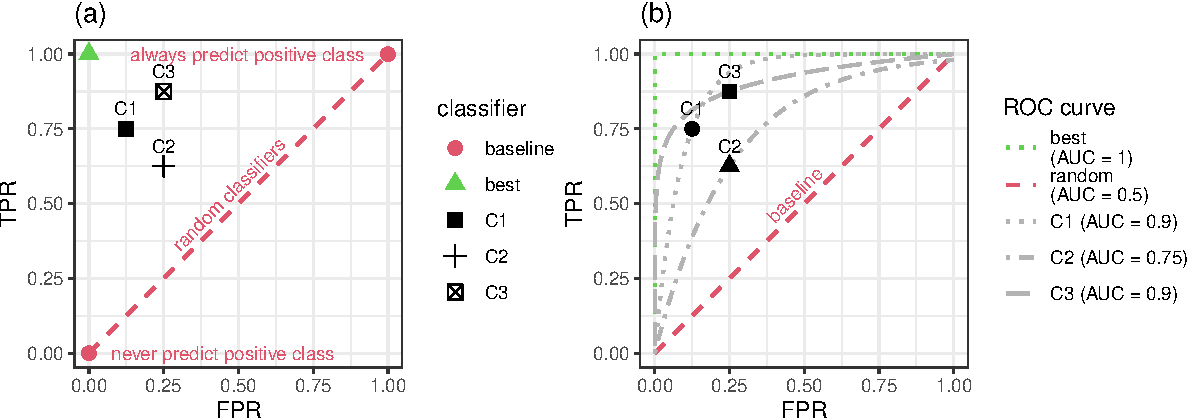
\includegraphics[width=1\textwidth,height=\textheight]{chapters/chapter3/evaluation_and_benchmarking_files/figure-pdf/fig-roc-1.pdf}

}

\caption{\label{fig-roc}Panel (a): ROC space with best discrete
classifier, two baseline classifiers -- one that always predicts the
positive class and one that never predicts the positive class -- and
three `real' classifiers C1, C2, C3. We cannot say if C1 or C3 is better
than the other as both are better in one metric. C2 is clearly worse
than C1 and C3, which are better in at least one metric than C2 while
not being worse in any other metric. Panel (b): ROC curves of the best
classifier (AUC = 1), of a random guessing classifier (AUC = 0.5), and
the classifiers C1, C3, and C2.}

\end{figure}

Now consider classifiers that predict probabilities instead of discrete
classes. Using different thresholds to cut off predicted probabilities
and assign them to the positive and negative class will lead to
different TPRs and FPRs and by plotting these values across different
thresholds we can characterize the behavior of a binary classifier --
this is the ROC curve. For example, we can use the previous
\href{https://mlr3.mlr-org.com/reference/Prediction.html}{\texttt{Prediction}}
object to compute all possible TPR and FPR combinations by thresholding
the predicted probabilities across all possible thresholds, which is
exactly what \texttt{mlr3viz::autoplot.PredictionClassif} will do when
\texttt{type\ =\ "roc"} is selected:

\begin{Shaded}
\begin{Highlighting}[]
\FunctionTok{autoplot}\NormalTok{(prediction, }\AttributeTok{type =} \StringTok{"roc"}\NormalTok{)}
\end{Highlighting}
\end{Shaded}

\begin{figure}

{\centering 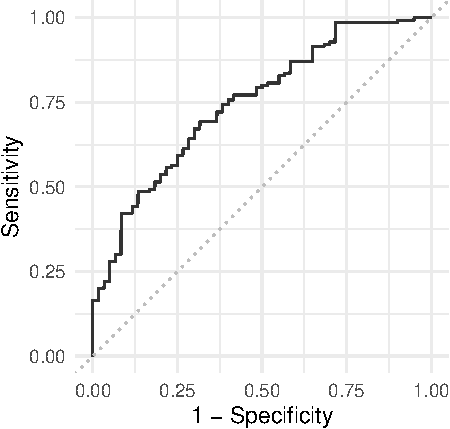
\includegraphics[width=0.7\textwidth,height=\textheight]{chapters/chapter3/evaluation_and_benchmarking_files/figure-pdf/fig-basics-roc-ranger-1.pdf}

}

\caption{\label{fig-basics-roc-ranger}ROC-curve based on the
\texttt{german\_credit} dataset and the \texttt{classif.ranger} random
forest learner. Recall FPR = \(1 -\) Specificity and TPR = Sensitivity.}

\end{figure}

A natural performance measure that can be derived from the ROC curve is
the area under the curve\index{AUC}{\marginnote{\begin{footnotesize}Area
Under the Curve\end{footnotesize}}} (AUC), implemented in
\texttt{msr("classif.auc")}. The AUC can be interpreted as the
probability that a randomly chosen positive instance has a higher
predicted probability of belonging to the positive class than a randomly
chosen negative instance. Therefore, higher values (closer to \(1\))
indicate better performance. Random classifiers (such as the featureless
baseline) will always have an AUC of (approximately, when evaluated
empirically) 0.5 (see Figure~\ref{fig-roc}, panel (b)).

\begin{Shaded}
\begin{Highlighting}[]
\NormalTok{prediction}\SpecialCharTok{$}\FunctionTok{score}\NormalTok{(}\FunctionTok{msr}\NormalTok{(}\StringTok{"classif.auc"}\NormalTok{))}
\end{Highlighting}
\end{Shaded}

\begin{verbatim}
classif.auc 
     0.7475 
\end{verbatim}

Evaluating our random forest on \texttt{tsk("german\_credit")} results
in an AUC of around 0.75, which is acceptable but could be better.

\begin{tcolorbox}[enhanced jigsaw, opacitybacktitle=0.6, rightrule=.15mm, opacityback=0, arc=.35mm, breakable, titlerule=0mm, colframe=quarto-callout-tip-color-frame, coltitle=black, bottomrule=.15mm, toprule=.15mm, colback=white, colbacktitle=quarto-callout-tip-color!10!white, bottomtitle=1mm, toptitle=1mm, title=\textcolor{quarto-callout-tip-color}{\faLightbulb}\hspace{0.5em}{Multiclass ROC and AUC}, leftrule=.75mm, left=2mm]

Extensions of ROC analysis for multiclass classifiers exist (see e.g.,
Hand and Till 2001) but we only cover the more common binary
classification case in this book. Generalizations of the AUC measure to
multiclass classification are implemented in \texttt{mlr3}, see
\texttt{msr("classif.mauc\_au1p")}.

\end{tcolorbox}

We can also plot the precision-recall
curve\index{precision-recall curve}{\marginnote{\begin{footnotesize}Precision-recall
Curve\end{footnotesize}}} (PRC) which visualizes the
PPV/precision\index{positive predictive value}
vs.~TPR/recall\index{true positive rate}. The main difference between
ROC curves and PR curves is that the number of true-negatives are
ignored in the latter. This can be useful in imbalanced populations
where the positive class is rare, and where a classifier with high TPR
may still not be very informative and have low PPV. See Davis and
Goadrich (2006) for a detailed discussion about the relationship between
the PRC and ROC curves.

\begin{Shaded}
\begin{Highlighting}[]
\FunctionTok{autoplot}\NormalTok{(prediction, }\AttributeTok{type =} \StringTok{"prc"}\NormalTok{)}
\end{Highlighting}
\end{Shaded}

\begin{figure}

{\centering 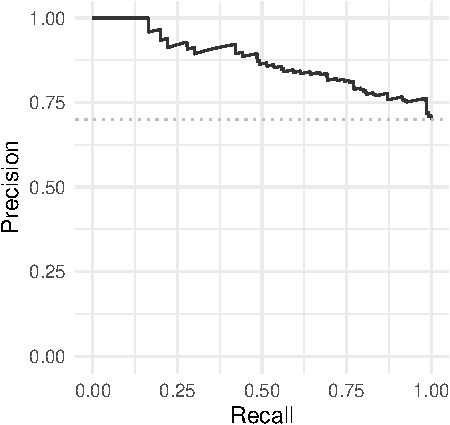
\includegraphics[width=0.7\textwidth,height=\textheight]{chapters/chapter3/evaluation_and_benchmarking_files/figure-pdf/fig-basics-prc-ranger-1.pdf}

}

\caption{\label{fig-basics-prc-ranger}Precision-Recall curve based on
\texttt{tsk("german\_credit")} and \texttt{lrn("classif.ranger")}.}

\end{figure}

Another useful way to think about the performance of a classifier is to
visualize the relationship of a performance metric over varying
thresholds, for example, see Figure~\ref{fig-basics-fpracc-ranger} to
inspect the FPR and accuracy across all possible thresholds:

\begin{Shaded}
\begin{Highlighting}[]
\FunctionTok{autoplot}\NormalTok{(prediction, }\AttributeTok{type =} \StringTok{"threshold"}\NormalTok{, }\AttributeTok{measure =} \FunctionTok{msr}\NormalTok{(}\StringTok{"classif.fpr"}\NormalTok{))}
\FunctionTok{autoplot}\NormalTok{(prediction, }\AttributeTok{type =} \StringTok{"threshold"}\NormalTok{, }\AttributeTok{measure =} \FunctionTok{msr}\NormalTok{(}\StringTok{"classif.acc"}\NormalTok{))}
\end{Highlighting}
\end{Shaded}

\begin{figure}

\begin{minipage}[t]{0.50\linewidth}

{\centering 

\raisebox{-\height}{

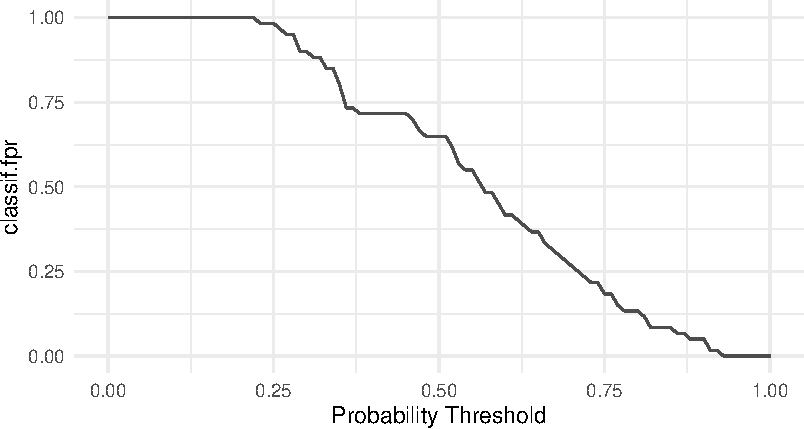
\includegraphics{chapters/chapter3/evaluation_and_benchmarking_files/figure-pdf/fig-basics-fpracc-ranger-1.pdf}

}

}

\subcaption{\label{fig-basics-fpracc-ranger-1}FPR}
\end{minipage}%
%
\begin{minipage}[t]{0.50\linewidth}

{\centering 

\raisebox{-\height}{

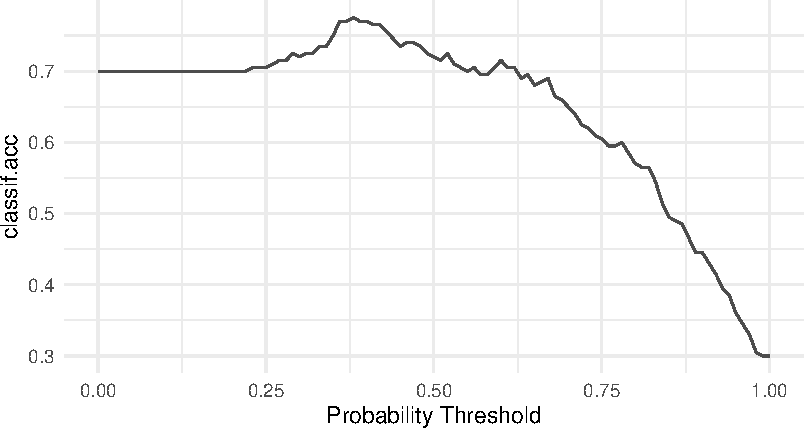
\includegraphics{chapters/chapter3/evaluation_and_benchmarking_files/figure-pdf/fig-basics-fpracc-ranger-2.pdf}

}

}

\subcaption{\label{fig-basics-fpracc-ranger-2}Accuracy}
\end{minipage}%

\caption{\label{fig-basics-fpracc-ranger}Comparing threshold and FPR
(left) with threshold and accuracy (right) for the random forest trained
on \texttt{tsk("german\_credit")}.}

\end{figure}

This visualization would show us that changing the threshold from the
default 0.5 to a higher value like 0.7 would greatly reduce the FPR
while reducing accuracy by only a few percentage points. Depending on
the problem at hand, this might be a perfectly desirable trade-off.

These visualizations are also available for
\href{https://mlr3.mlr-org.com/reference/ResampleResult.html}{\texttt{ResampleResult}}
objects. In this case, the predictions of individual resampling
iterations are merged before calculating a ROC or PR curve (micro
averaged):

\begin{Shaded}
\begin{Highlighting}[]
\NormalTok{rr }\OtherTok{=} \FunctionTok{resample}\NormalTok{(}
  \AttributeTok{task =} \FunctionTok{tsk}\NormalTok{(}\StringTok{"german\_credit"}\NormalTok{),}
  \AttributeTok{learner =} \FunctionTok{lrn}\NormalTok{(}\StringTok{"classif.ranger"}\NormalTok{, }\AttributeTok{predict\_type =} \StringTok{"prob"}\NormalTok{),}
  \AttributeTok{resampling =} \FunctionTok{rsmp}\NormalTok{(}\StringTok{"cv"}\NormalTok{, }\AttributeTok{folds =} \DecValTok{5}\NormalTok{)}
\NormalTok{)}
\FunctionTok{autoplot}\NormalTok{(rr, }\AttributeTok{type =} \StringTok{"roc"}\NormalTok{)}
\FunctionTok{autoplot}\NormalTok{(rr, }\AttributeTok{type =} \StringTok{"prc"}\NormalTok{)}
\end{Highlighting}
\end{Shaded}

\begin{figure}

\begin{minipage}[t]{0.50\linewidth}

{\centering 

\raisebox{-\height}{

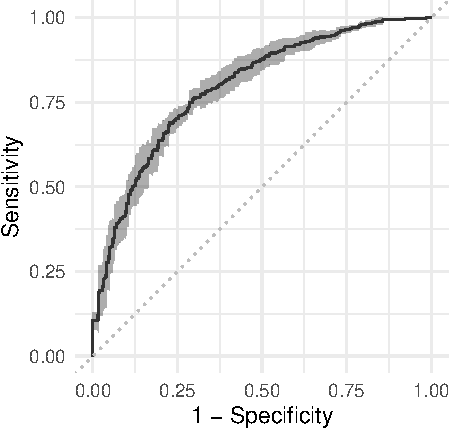
\includegraphics{chapters/chapter3/evaluation_and_benchmarking_files/figure-pdf/fig-basics-rocpr-ranger-1.pdf}

}

}

\subcaption{\label{fig-basics-rocpr-ranger-1}ROC}
\end{minipage}%
%
\begin{minipage}[t]{0.50\linewidth}

{\centering 

\raisebox{-\height}{

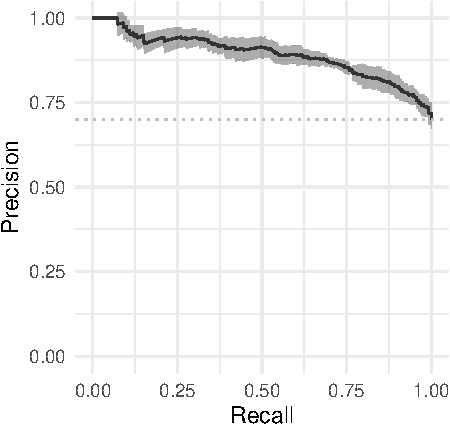
\includegraphics{chapters/chapter3/evaluation_and_benchmarking_files/figure-pdf/fig-basics-rocpr-ranger-2.pdf}

}

}

\subcaption{\label{fig-basics-rocpr-ranger-2}PR Curve}
\end{minipage}%

\caption{\label{fig-basics-rocpr-ranger}Comparing ROC (left) and PR
curve (right) for a random forest trained on
\texttt{tsk("german\_credit")}.}

\end{figure}

Finally, we can visualize ROC/PR curves for a
\href{https://mlr3.mlr-org.com/reference/BenchmarkResult.html}{\texttt{BenchmarkResult}}
to compare multiple learners on the same
\href{https://mlr3.mlr-org.com/reference/Task.html}{\texttt{Task}}:

\begin{Shaded}
\begin{Highlighting}[]
\FunctionTok{library}\NormalTok{(patchwork)}

\NormalTok{design }\OtherTok{=} \FunctionTok{benchmark\_grid}\NormalTok{(}
  \AttributeTok{tasks =} \FunctionTok{tsk}\NormalTok{(}\StringTok{"german\_credit"}\NormalTok{),}
  \AttributeTok{learners =} \FunctionTok{lrns}\NormalTok{(}\FunctionTok{c}\NormalTok{(}\StringTok{"classif.rpart"}\NormalTok{, }\StringTok{"classif.ranger"}\NormalTok{),}
    \AttributeTok{predict\_type =} \StringTok{"prob"}\NormalTok{),}
  \AttributeTok{resamplings =} \FunctionTok{rsmp}\NormalTok{(}\StringTok{"cv"}\NormalTok{, }\AttributeTok{folds =} \DecValTok{5}\NormalTok{)}
\NormalTok{)}
\NormalTok{bmr }\OtherTok{=} \FunctionTok{benchmark}\NormalTok{(design)}
\FunctionTok{autoplot}\NormalTok{(bmr, }\AttributeTok{type =} \StringTok{"roc"}\NormalTok{) }\SpecialCharTok{+} \FunctionTok{autoplot}\NormalTok{(bmr, }\AttributeTok{type =} \StringTok{"prc"}\NormalTok{) }\SpecialCharTok{+}
  \FunctionTok{plot\_layout}\NormalTok{(}\AttributeTok{guides =} \StringTok{"collect"}\NormalTok{)}
\end{Highlighting}
\end{Shaded}

\begin{figure}

{\centering 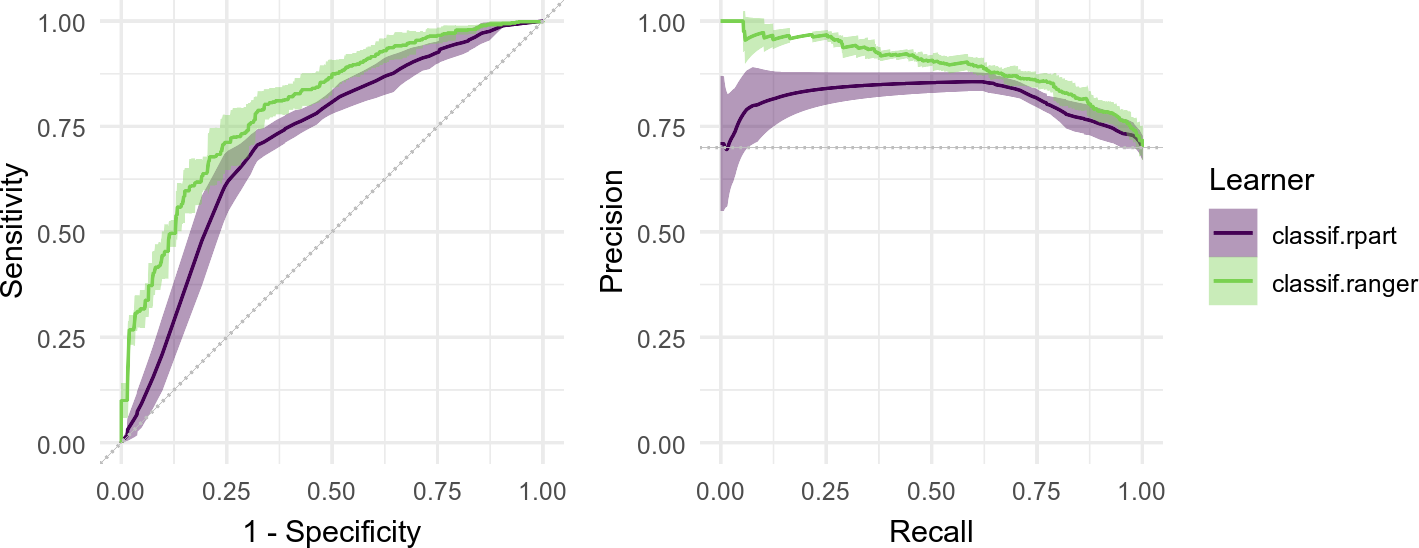
\includegraphics[width=1\textwidth,height=\textheight]{chapters/chapter3/evaluation_and_benchmarking_files/figure-pdf/fig-basics-rocpr-bmr-1.png}

}

\caption{\label{fig-basics-rocpr-bmr}Comparing random forest (green) and
decision tree (purple) using ROC and PR Curves.}

\end{figure}

\hypertarget{conclusion-1}{%
\section{Conclusion}\label{conclusion-1}}

In this chapter, we learned how to estimate the generalization
performance of a model via resampling strategies, from holdout to
cross-validation and bootstrap, and how to automate the comparison of
multiple learners in benchmark experiments. We also covered the basics
of performance measures for binary classification, including the
confusion matrix, ROC analysis, and precision-recall curves. These
topics are fundamental in supervised learning and will continue to be
built upon throughout this book. In particular,
Chapter~\ref{sec-optimization} utilizes evaluation in automated model
tuning to improve performance, in Chapter~\ref{sec-large-benchmarking}
we look at large benchmarks and their statistical analysis, and in
Chapter~\ref{sec-special} we will take a look at specialized tasks that
require different resampling strategies.

\hypertarget{tbl-api-performance}{}
\begin{longtable}[]{@{}
  >{\raggedright\arraybackslash}p{(\columnwidth - 4\tabcolsep) * \real{0.2353}}
  >{\raggedright\arraybackslash}p{(\columnwidth - 4\tabcolsep) * \real{0.2941}}
  >{\raggedright\arraybackslash}p{(\columnwidth - 4\tabcolsep) * \real{0.4706}}@{}}
\caption{\label{tbl-api-performance}Important classes and functions
covered in this chapter with underlying class (if applicable), class
constructor or function, and important class fields and methods (if
applicable).}\tabularnewline
\toprule\noalign{}
\begin{minipage}[b]{\linewidth}\raggedright
Class
\end{minipage} & \begin{minipage}[b]{\linewidth}\raggedright
Constructor/Function
\end{minipage} & \begin{minipage}[b]{\linewidth}\raggedright
Fields/Methods
\end{minipage} \\
\midrule\noalign{}
\endfirsthead
\toprule\noalign{}
\begin{minipage}[b]{\linewidth}\raggedright
Class
\end{minipage} & \begin{minipage}[b]{\linewidth}\raggedright
Constructor/Function
\end{minipage} & \begin{minipage}[b]{\linewidth}\raggedright
Fields/Methods
\end{minipage} \\
\midrule\noalign{}
\endhead
\bottomrule\noalign{}
\endlastfoot
\href{https://mlr3.mlr-org.com/reference/PredictionClassif.html}{\texttt{PredictionClassif}}
& \texttt{classif\_lrn\$predict()} &
\href{https://www.rdocumentation.org/packages/mlr3measures/topics/confusion_matrix}{\texttt{confusion\_matrix()}};
\texttt{autoplot(some\_prediction\_classif,\ type\ =\ "roc")} \\
- &
\href{https://mlr3.mlr-org.com/reference/partition.html}{\texttt{partition()}}
& - \\
\href{https://mlr3.mlr-org.com/reference/Resampling.html}{\texttt{Resampling}}
&
\href{https://mlr3.mlr-org.com/reference/mlr_sugar.html}{\texttt{rsmp()}}
& \texttt{\$instantiate()} \\
\href{https://mlr3.mlr-org.com/reference/ResampleResult.html}{\texttt{ResampleResult}}
&
\href{https://mlr3.mlr-org.com/reference/resample.html}{\texttt{resample()}}
& \texttt{\$score()}; \texttt{\$aggregate()}; \texttt{\$predictions()};
\texttt{as\_benchmark\_result()};
\texttt{autoplot(some\_resample\_result,\ type\ =\ "roc")} \\
- &
\href{https://mlr3.mlr-org.com/reference/benchmark_grid.html}{\texttt{benchmark\_grid()}}
& - \\
\href{https://mlr3.mlr-org.com/reference/BenchmarkResult.html}{\texttt{BenchmarkResult}}
&
\href{https://mlr3.mlr-org.com/reference/benchmark.html}{\texttt{benchmark()}}
& \texttt{\$aggregate()}; \texttt{\$resample\_result()};
\texttt{\$score()};
\texttt{autoplot(some\_benchmark\_result,\ type\ =\ "roc")} \\
\end{longtable}

\hypertarget{exercises-1}{%
\section{Exercises}\label{exercises-1}}

\begin{enumerate}
\def\labelenumi{\arabic{enumi}.}
\item
  Apply a repeated cross-validation resampling strategy on
  \texttt{tsk("mtcars")} and evaluate the performance of
  \texttt{lrn("regr.rpart")}. Use five repeats of three folds each.
  Calculate the MSE for each iteration and visualize the result.
  Finally, calculate the aggregated performance score.
\item
  Use \texttt{tsk("spam")} and five-fold CV to benchmark
  \texttt{lrn("classif.ranger")}, \texttt{lrn("classif.log\_reg")}, and
  \texttt{lrn("classif.xgboost")} with respect to AUC. Which learner
  appears to perform best? How confident are you in your conclusion?
  Think about the stability of results and investigate this by
  re-rerunning the experiment with different seeds. What can be done to
  improve this?
\item
  A colleague reports a 93.1\% classification accuracy using
  \texttt{lrn("classif.rpart")} on \texttt{tsk("penguins\_simple")}. You
  want to reproduce their results and ask them about their resampling
  strategy. They said they used a custom three-fold CV with folds
  assigned as \texttt{factor(task\$row\_ids\ \%\%\ 3)}. See if you can
  reproduce their results.
\item
  (*) Program your own ROC plotting function without using
  \texttt{mlr3}'s \texttt{autoplot()} function. The signature of your
  function should be
  \texttt{my\_roc\_plot(task,\ learner,\ train\_indices,\ test\_indices)}.
  Your function should use the \texttt{\$set\_threshold()} method of
  \texttt{Prediction}, as well as \texttt{mlr3measures}.
\end{enumerate}


\part{Tuning and Feature Selection}

\hypertarget{sec-optimization}{%
\chapter{Hyperparameter Optimization}\label{sec-optimization}}

\vspace{-15mm}\addtocontents{toc}{\textit{Marc Becker, Lennart Schneider and Sebastian Fischer}}

\textbf{Marc Becker} \newline  \emph{Ludwig-Maximilians-Universität
München, and Munich Center for Machine Learning (MCML)}

\textbf{Lennart Schneider} \newline 
\emph{Ludwig-Maximilians-Universität München, and Munich Center for
Machine Learning (MCML)}

\textbf{Sebastian Fischer} \newline 
\emph{Ludwig-Maximilians-Universität München, and Munich Center for
Machine Learning (MCML)} \newline \newline 

Machine learning algorithms usually include parameters\index{parameters}
and
hyperparameters\index{hyperparameters}{\marginnote{\begin{footnotesize}Hyperparameters\end{footnotesize}}}.
Parameters are the model
coefficients\index{model coefficients|see{parameters}} or weights or
other information that are determined by the learning algorithm based on
the training data. In contrast, hyperparameters, are configured by the
user and determine how the model will fit its parameters, i.e., how the
model is built. Examples include setting the number of trees in a random
forest, penalty settings in support vector machines, or the learning
rate in a neural network.

The goal of hyperparameter
optimization\index{HPO}{\marginnote{\begin{footnotesize}Hyperparameter
Optimization\end{footnotesize}}}\index{hyperparameter optimization|see{HPO}}
(HPO) or model tuning\index{tuning} is to find the optimal configuration
of hyperparameters of a machine learning algorithm for a given task.
There is no closed-form mathematical representation (nor analytic
gradient information) for model-agnostic HPO. Instead, we follow a black
box optimization\index{black box optimization} approach: a machine
learning algorithm is configured with values chosen for one or more
hyperparameters, this algorithm is then evaluated (using a resampling
method) and its performance is measured. This process is repeated with
multiple configurations and finally, the configuration with the best
performance is selected (Figure~\ref{fig-optimization-loop-basic}). HPO
closely relates to model evaluation\index{model evaluation}
(Chapter~\ref{sec-performance}) as the objective is to find a
hyperparameter configuration that optimizes the generalization
performance. Broadly speaking, we could think of finding the optimal
model configuration in the same way as selecting a model from a
benchmark experiment, where in this case each model in the experiment is
the same algorithm but with different hyperparameter configurations. For
example, we could benchmark three support vector
machines\index{support vector machine} (SVMs) with three different
\texttt{cost} values. However, human trial-and-error is time-consuming,
subjective and often biased, error-prone, and computationally
inefficient. Instead, many sophisticated hyperparameter optimization
methods (or `tuners\index{tuners}', see Section~\ref{sec-tuner}) have
been developed over the past few decades for robust and efficient HPO.
Besides simple approaches such as a random search\index{random search}
or grid search\index{grid search}, most hyperparameter optimization
methods employ iterative techniques that propose different
configurations over time, often exhibiting adaptive behavior guided
towards potentially optimal hyperparameter configurations. These methods
continually propose new configurations until a termination criterion is
met, at which point the best configuration so far is returned
(Figure~\ref{fig-optimization-loop-basic}). For more general details on
HPO and more theoretical background, we recommend Bischl et al. (2023)
and Feurer and Hutter (2019).

\begin{figure}

{\centering \includegraphics[width=0.8\textwidth]{chapters/chapter4/Figures/mlr3book_figures-9.png}

}

\caption{\label{fig-optimization-loop-basic}Representation of the
hyperparameter optimization loop in mlr3tuning. Blue - Hyperparameter
optimization loop. Purple - Objects of the tuning instance supplied by
the user. Blue-Green - Internally created objects of the tuning
instance. Green - Optimization Algorithm.}

\end{figure}

\hypertarget{sec-model-tuning}{%
\section{Model Tuning}\label{sec-model-tuning}}

\href{https://mlr3tuning.mlr-org.com}{\texttt{mlr3tuning}}\index{\texttt{mlr3tuning}}
is the hyperparameter optimization package of the \texttt{mlr3}
ecosystem. At the heart of the package are the R6 classes

\begin{itemize}
\tightlist
\item
  \href{https://mlr3tuning.mlr-org.com/reference/TuningInstanceSingleCrit.html}{\texttt{TuningInstanceSingleCrit}},
  a tuning `instance' that describes the optimization problem and store
  the results; and
\item
  \href{https://mlr3tuning.mlr-org.com/reference/Tuner.html}{\texttt{Tuner}}
  which is used to configure and run optimization algorithms.
\end{itemize}

In this section, we will cover these classes as well as other supporting
functions and classes. Throughout this section, we will look at
optimizing an SVM classifier\index{support vector machine} from
\href{https://cran.r-project.org/package=e1071}{\texttt{e1071}} on
\texttt{tsk("sonar")} as a running example.

\hypertarget{sec-learner-search-space}{%
\subsection{Learner and Search Space}\label{sec-learner-search-space}}

The tuning process begins by deciding which hyperparameters to tune and
what range to tune them over. The first place to start is therefore
picking a learner and looking at the possible hyperparameters to tune
with \texttt{\$param\_set}:

\begin{Shaded}
\begin{Highlighting}[]
\FunctionTok{as.data.table}\NormalTok{(}\FunctionTok{lrn}\NormalTok{(}\StringTok{"classif.svm"}\NormalTok{)}\SpecialCharTok{$}\NormalTok{param\_set)[,}
\NormalTok{  .(id, class, lower, upper, nlevels)]}
\end{Highlighting}
\end{Shaded}

\begin{verbatim}
               id    class lower upper nlevels
 1:     cachesize ParamDbl  -Inf   Inf     Inf
 2: class.weights ParamUty    NA    NA     Inf
 3:         coef0 ParamDbl  -Inf   Inf     Inf
 4:          cost ParamDbl     0   Inf     Inf
 5:         cross ParamInt     0   Inf     Inf
---                                           
12:            nu ParamDbl  -Inf   Inf     Inf
13:         scale ParamUty    NA    NA     Inf
14:     shrinking ParamLgl    NA    NA       2
15:     tolerance ParamDbl     0   Inf     Inf
16:          type ParamFct    NA    NA       2
\end{verbatim}

Given infinite resources, we could tune all hyperparameters jointly, but
in reality that is not possible (or maybe necessary), so usually only a
subset of hyperparameters can be tuned. This subset of possible
hyperparameter values to tune over is referred to as the search
space\index{search space}{\marginnote{\begin{footnotesize}Search
Space\end{footnotesize}}} or tuning
space\index{tuning space|see{search space}}. In this example we will
tune the numeric regularization and kernel width hyperparameters,
\texttt{cost} and \texttt{gamma}; see the help page for
\href{https://www.rdocumentation.org/packages/e1071/topics/svm}{\texttt{svm()}}
for details. In practice, search spaces are usually more complex and can
require expert knowledge to define them.
Section~\ref{sec-defining-search-spaces} provides more detailed insight
into the creation of tuning spaces, including using
\href{https://mlr3tuningspaces.mlr-org.com}{\texttt{mlr3tuningspaces}}\index{\texttt{mlr3tuningspaces}}
to load predefined search spaces.

\begin{tcolorbox}[enhanced jigsaw, opacitybacktitle=0.6, rightrule=.15mm, opacityback=0, arc=.35mm, breakable, titlerule=0mm, colframe=quarto-callout-tip-color-frame, coltitle=black, bottomrule=.15mm, toprule=.15mm, colback=white, colbacktitle=quarto-callout-tip-color!10!white, bottomtitle=1mm, toptitle=1mm, title=\textcolor{quarto-callout-tip-color}{\faLightbulb}\hspace{0.5em}{Untunable Hyperparameters}, leftrule=.75mm, left=2mm]

In rare cases, parameter sets may include hyperparameters that should
not be tuned. These will usually be `technical' (or `control')
parameters that \emph{provide information} about how the model is being
fit but do not control the training process itself, for example, the
\texttt{verbose} hyperparameter in \texttt{lrn("classif.ranger")}
controls how much information is displayed to the user during training.

\end{tcolorbox}

For numeric hyperparameters (we will explore others later) one must
specify the bounds to tune over. We do this by constructing a learner
and using
\href{https://paradox.mlr-org.com/reference/to_tune.html}{\texttt{to\_tune()}}
to set the lower and upper limits for the parameters we want to tune.
This function allows us to \emph{mark} the hyperparameter as requiring
tuning in the specified range.

\begin{Shaded}
\begin{Highlighting}[]
\NormalTok{learner }\OtherTok{=} \FunctionTok{lrn}\NormalTok{(}\StringTok{"classif.svm"}\NormalTok{,}
  \AttributeTok{type  =} \StringTok{"C{-}classification"}\NormalTok{,}
  \AttributeTok{kernel =} \StringTok{"radial"}\NormalTok{,}
  \AttributeTok{cost  =} \FunctionTok{to\_tune}\NormalTok{(}\FloatTok{1e{-}1}\NormalTok{, }\FloatTok{1e5}\NormalTok{),}
  \AttributeTok{gamma =} \FunctionTok{to\_tune}\NormalTok{(}\FloatTok{1e{-}1}\NormalTok{, }\DecValTok{1}\NormalTok{)}
\NormalTok{)}
\NormalTok{learner}
\end{Highlighting}
\end{Shaded}

\begin{verbatim}
<LearnerClassifSVM:classif.svm>
* Model: -
* Parameters: type=C-classification, kernel=radial,
  cost=<RangeTuneToken>, gamma=<RangeTuneToken>
* Packages: mlr3, mlr3learners, e1071
* Predict Types:  [response], prob
* Feature Types: logical, integer, numeric
* Properties: multiclass, twoclass
\end{verbatim}

Here we have constructed a classification SVM,
\texttt{lrn("classif.svm")}, selected the type of model as
\texttt{"C-classification"}, set the kernel to \texttt{"radial"}, and
specified that we plan to tune the \texttt{cost} and \texttt{gamma}
parameters over the range \([0.1, 10^5]\) and \([0.1, 1]\) respectively
(though these are usually tuned on a log scale, see
Section~\ref{sec-logarithmic-transformations}). Note that calling
\texttt{\$train()} on a learner with a tune token (e.g.,
\texttt{cost=\textless{}RangeTuneToken\textgreater{}}) will throw an
error.

Now we have decided which hyperparameters to tune, we specify when to
stop the tuning process.

\hypertarget{sec-terminator}{%
\subsection{Terminator}\label{sec-terminator}}

\texttt{mlr3tuning} includes many methods to specify when to terminate
an algorithm (Table~\ref{tbl-terms}), which are implemented in
\href{https://bbotk.mlr-org.com/reference/Terminator.html}{\texttt{Terminator}}\index{\texttt{Terminator}}{\marginnote{\begin{footnotesize}\texttt{Terminator}\end{footnotesize}}}
classes. Terminators are stored in the
\href{https://bbotk.mlr-org.com/reference/mlr_terminators.html}{\texttt{mlr\_terminators}}
dictionary and are constructed with the sugar function
\href{https://bbotk.mlr-org.com/reference/trm.html}{\texttt{trm()}}\index{\texttt{trm()}}{\marginnote{\begin{footnotesize}\texttt{trm()}\end{footnotesize}}}.

\hypertarget{tbl-terms}{}
\begin{longtable}[]{@{}
  >{\raggedright\arraybackslash}p{(\columnwidth - 2\tabcolsep) * \real{0.2396}}
  >{\raggedright\arraybackslash}p{(\columnwidth - 2\tabcolsep) * \real{0.7604}}@{}}
\caption{\label{tbl-terms}Terminators available in \texttt{mlr3tuning}
at the time of publication, their function call and default parameters.
A complete and up-to-date list can be found at
\url{https://mlr-org.com/terminators.html}.}\tabularnewline
\toprule\noalign{}
\begin{minipage}[b]{\linewidth}\raggedright
Terminator
\end{minipage} & \begin{minipage}[b]{\linewidth}\raggedright
Function call and default parameters
\end{minipage} \\
\midrule\noalign{}
\endfirsthead
\toprule\noalign{}
\begin{minipage}[b]{\linewidth}\raggedright
Terminator
\end{minipage} & \begin{minipage}[b]{\linewidth}\raggedright
Function call and default parameters
\end{minipage} \\
\midrule\noalign{}
\endhead
\bottomrule\noalign{}
\endlastfoot
Clock Time & \texttt{trm("clock\_time")} \\
Combo & \texttt{trm("combo",\ any\ =\ TRUE)} \\
None & \texttt{trm("none")} \\
Number of Evaluations &
\texttt{trm("evals",\ n\_evals\ =\ 100,\ k\ =\ 0)} \\
Performance Level & \texttt{trm("perf\_reached",\ level\ =\ 0.1)} \\
Run Time & \texttt{trm("run\_time",\ secs\ =\ 30)} \\
Stagnation &
\texttt{trm("stagnation",\ iters\ =\ 10,\ threshold\ =\ 0)} \\
\end{longtable}

The most commonly used terminators are those that stop the tuning after
a certain time (\texttt{trm("run\_time")}) or a given number of
evaluations (\texttt{trm("evals")}). Choosing a runtime is often based
on practical considerations and intuition. Using a time limit can be
important on compute clusters where a maximum runtime for a compute job
may need to be specified. \texttt{trm("perf\_reached")} stops the tuning
when a specified performance level is reached, which can be helpful if a
certain performance is seen as sufficient for the practical use of the
model, however, if this is set too optimistically the tuning may never
terminate. \texttt{trm("stagnation")} stops when no progress greater
than the \texttt{threshold} has been made for a set number of
\texttt{iterations}. The threshold can be difficult to select as the
optimization could stop too soon for complex search spaces despite room
for (possibly significant) improvement. \texttt{trm("none")} is used for
tuners that control termination themselves and so this terminator does
nothing. Finally, any of these terminators can be freely combined by
using \texttt{trm("combo")}, which can be used to specify if HPO
finishes when any (\texttt{any\ =\ TRUE}) terminator is triggered or
when all (\texttt{any\ =\ FALSE}) are triggered.

\hypertarget{sec-tuning-instance}{%
\subsection{\texorpdfstring{Tuning Instance with
\texttt{ti}}{Tuning Instance with ti}}\label{sec-tuning-instance}}

The tuning instance collects the tuner-agnostic information required to
optimize a model, i.e., all information about the tuning process, except
for the tuning algorithm itself. This includes the task to tune over,
the learner to tune, the resampling method and measure used to
analytically compare hyperparameter optimization configurations, and the
terminator to determine when the measure has been optimized `enough'.
This implicitly defines a ``black box'' objective function, mapping
hyperparameter configurations to (stochastic) performance values, to be
optimized. This concept will be revisited in
Chapter~\ref{sec-optimization-advanced}.

A tuning instance\index{tuning instance} can be constructed explicitly
with the
\href{https://mlr3tuning.mlr-org.com/reference/ti.html}{\texttt{ti()}}
function, or we can tune a learner with the
\href{https://mlr3tuning.mlr-org.com/reference/tune.html}{\texttt{tune()}}
function, which implicitly creates a tuning instance, as shown in
Section~\ref{sec-autotuner}. We cover the \texttt{ti()} approach first
as this allows finer control of tuning and a more nuanced discussion
about the design and use of \texttt{mlr3tuning}.

Continuing our example, we will construct a
single-objective\index{single-objective} tuning problem (i.e., tuning
over \emph{one} measure) by using the \texttt{ti()} function to create a
\href{https://mlr3tuning.mlr-org.com/reference/TuningInstanceSingleCrit.html}{\texttt{TuningInstanceSingleCrit}},
we will return to multi-objective tuning\index{multi-objective tuning}
in Section~\ref{sec-multi-metrics-tuning}.

For this example, we will use three-fold CV and optimize the
classification error measure. Note that in the next section, we will
continue our example with a grid search tuner, so we select
\texttt{trm("none")} below as we will want to iterate over the full grid
without stopping too soon.

\begin{Shaded}
\begin{Highlighting}[]
\NormalTok{tsk\_sonar }\OtherTok{=} \FunctionTok{tsk}\NormalTok{(}\StringTok{"sonar"}\NormalTok{)}

\NormalTok{learner }\OtherTok{=} \FunctionTok{lrn}\NormalTok{(}\StringTok{"classif.svm"}\NormalTok{,}
  \AttributeTok{cost  =} \FunctionTok{to\_tune}\NormalTok{(}\FloatTok{1e{-}1}\NormalTok{, }\FloatTok{1e5}\NormalTok{),}
  \AttributeTok{gamma =} \FunctionTok{to\_tune}\NormalTok{(}\FloatTok{1e{-}1}\NormalTok{, }\DecValTok{1}\NormalTok{),}
  \AttributeTok{kernel =} \StringTok{"radial"}\NormalTok{,}
  \AttributeTok{type =} \StringTok{"C{-}classification"}
\NormalTok{)}

\NormalTok{instance }\OtherTok{=} \FunctionTok{ti}\NormalTok{(}
  \AttributeTok{task =}\NormalTok{ tsk\_sonar,}
  \AttributeTok{learner =}\NormalTok{ learner,}
  \AttributeTok{resampling =} \FunctionTok{rsmp}\NormalTok{(}\StringTok{"cv"}\NormalTok{, }\AttributeTok{folds =} \DecValTok{3}\NormalTok{),}
  \AttributeTok{measures =} \FunctionTok{msr}\NormalTok{(}\StringTok{"classif.ce"}\NormalTok{),}
  \AttributeTok{terminator =} \FunctionTok{trm}\NormalTok{(}\StringTok{"none"}\NormalTok{)}
\NormalTok{)}

\NormalTok{instance}
\end{Highlighting}
\end{Shaded}

\begin{verbatim}
<TuningInstanceSingleCrit>
* State:  Not optimized
* Objective: <ObjectiveTuning:classif.svm_on_sonar>
* Search Space:
      id    class lower upper nlevels
1:  cost ParamDbl   0.1 1e+05     Inf
2: gamma ParamDbl   0.1 1e+00     Inf
* Terminator: <TerminatorNone>
\end{verbatim}

\hypertarget{sec-tuner}{%
\subsection{Tuner}\label{sec-tuner}}

With all the pieces of our tuning problem assembled, we can now decide
\emph{how} to tune our model. There are multiple
\href{https://mlr3tuning.mlr-org.com/reference/Tuner.html}{\texttt{Tuner}}\index{\texttt{Tuner}}{\marginnote{\begin{footnotesize}\texttt{Tuner}\end{footnotesize}}}
classes in \texttt{mlr3tuning}, which implement different HPO (or more
generally speaking black box optimization\index{black box optimization})
algorithms (Table~\ref{tbl-tuners}).

\hypertarget{tbl-tuners}{}
\begin{longtable}[]{@{}
  >{\raggedright\arraybackslash}p{(\columnwidth - 4\tabcolsep) * \real{0.4125}}
  >{\raggedright\arraybackslash}p{(\columnwidth - 4\tabcolsep) * \real{0.3000}}
  >{\raggedright\arraybackslash}p{(\columnwidth - 4\tabcolsep) * \real{0.2875}}@{}}
\caption{\label{tbl-tuners}Tuning algorithms available in
\texttt{mlr3tuning}, their function call and the package in which the
algorithm is implemented. A complete and up-to-date list can be found at
\url{https://mlr-org.com/tuners.html}.}\tabularnewline
\toprule\noalign{}
\begin{minipage}[b]{\linewidth}\raggedright
Tuner
\end{minipage} & \begin{minipage}[b]{\linewidth}\raggedright
Function call
\end{minipage} & \begin{minipage}[b]{\linewidth}\raggedright
Package
\end{minipage} \\
\midrule\noalign{}
\endfirsthead
\toprule\noalign{}
\begin{minipage}[b]{\linewidth}\raggedright
Tuner
\end{minipage} & \begin{minipage}[b]{\linewidth}\raggedright
Function call
\end{minipage} & \begin{minipage}[b]{\linewidth}\raggedright
Package
\end{minipage} \\
\midrule\noalign{}
\endhead
\bottomrule\noalign{}
\endlastfoot
Random Search & \texttt{tnr("random\_search")} &
\href{https://mlr3tuning.mlr-org.com}{\texttt{mlr3tuning}}\index{\texttt{mlr3tuning}} \\
Grid Search & \texttt{tnr("grid\_search")} &
\href{https://mlr3tuning.mlr-org.com}{\texttt{mlr3tuning}}\index{\texttt{mlr3tuning}} \\
Bayesian Optimization & \texttt{tnr("mbo")} &
\href{https://mlr3mbo.mlr-org.com}{\texttt{mlr3mbo}}\index{\texttt{mlr3mbo}} \\
CMA-ES & \texttt{tnr("cmaes")} &
\href{https://cran.r-project.org/package=adagio}{\texttt{adagio}} \\
Iterated Racing & \texttt{tnr("irace")} &
\href{https://cran.r-project.org/package=irace}{\texttt{irace}} \\
Hyperband & \texttt{tnr("hyperband")} &
\href{https://mlr3hyperband.mlr-org.com}{\texttt{mlr3hyperband}}\index{\texttt{mlr3hyperband}} \\
Generalized Simulated Annealing & \texttt{tnr("gensa")} &
\href{https://cran.r-project.org/package=GenSA}{\texttt{GenSA}} \\
Nonlinear Optimization & \texttt{tnr("nloptr")} &
\href{https://cran.r-project.org/package=nloptr}{\texttt{nloptr}} \\
\end{longtable}

\hypertarget{search-strategies}{%
\subsubsection*{Search strategies}\label{search-strategies}}

Grid search and random search (Bergstra and Bengio 2012) are the most
basic algorithms and are often selected first in initial experiments.
The idea of grid search is to exhaustively evaluate every possible
combination of given hyperparameter values. Categorical hyperparameters
are usually evaluated over all possible values they can take. Numeric
and integer hyperparameter values are then spaced equidistantly in their
box constraints (upper and lower bounds) according to a given
resolution, which is the number of distinct values to try per
hyperparameter. Random search involves randomly selecting values for
each hyperparameter independently from a pre-specified distribution,
usually uniform. Both methods are non-adaptive, which means each
proposed configuration ignores the performance of previous
configurations. Due to their simplicity, both grid search and random
search can handle mixed search spaces (i.e., hyperparameters can be
numeric, integer, or categorical) as well as hierarchical search spaces
(Section~\ref{sec-defining-search-spaces}).

\hypertarget{adaptive-algorithms}{%
\subsubsection*{Adaptive algorithms}\label{adaptive-algorithms}}

Adaptive algorithms learn from previously evaluated configurations to
find good configurations quickly, examples in
\href{https://mlr3.mlr-org.com}{\texttt{mlr3}}\index{\texttt{mlr3}}
include Bayesian optimization (also called model-based optimization),
Covariance Matrix Adaptation Evolution Strategy (CMA-ES), Iterated
Racing\index{iterated racing}, and Hyperband.

Bayesian optimization\index{Bayesian optimization} (e.g., Snoek,
Larochelle, and Adams 2012) describes a family of iterative optimization
algorithms that use a surrogate model to approximate the unknown
function that is to be optimized -- in HPO this would be the mapping
from a hyperparameter configuration to the estimated generalization
performance. If a suitable surrogate model is chosen, e.g.~a random
forest, Bayesian optimization can be quite flexible and even handle
mixed and hierarchical search spaces. Bayesian optimization is discussed
in full detail in Section~\ref{sec-bayesian-optimization}.

CMA-ES\index{CMA-ES} (Hansen and Auger 2011) is an evolutionary
strategy\index{evolutionary strategies} that maintains a probability
distribution over candidate points, with the distribution represented by
a mean vector and covariance matrix. A new set of candidate points is
generated by sampling from this distribution, with the probability of
each candidate being proportional to its performance. The covariance
matrix is adapted over time to reflect the performance landscape.
Further evolutionary strategies are available in \texttt{mlr3} via the
\href{https://cran.r-project.org/package=miesmuschel}{\texttt{miesmuschel}}
package, however, these will not be covered in this book.

Racing algorithms work by iteratively discarding configurations that
show poor performance, as determined by statistical tests. Iterated Racing (López-Ibáñez et al. 2016) starts by `racing' down an initial
population of randomly sampled configurations from a parameterized
density and then uses the surviving configurations of the race to
stochastically update the density of the subsequent race to focus on
promising regions of the search space, and so on.

Multi-fidelity HPO is an adaptive method that leverages the predictive
power of computationally cheap lower fidelity evaluations (i.e., poorer
quality predictions such as those arising from neural networks with a
small number of epochs) to improve the overall optimization efficiency.
This concept is used in Hyperband\index{hyperband} (Li et al. 2018), a
popular multi-fidelity hyperparameter optimization algorithm that
dynamically allocates increasingly more resources to promising
configurations and terminates low-performing ones. Hyperband is
discussed in full detail in Section~\ref{sec-hyperband}.

Other implemented algorithms for numeric search spaces are Generalized
Simulated Annealing (Xiang et al. 2013; Tsallis and Stariolo 1996) and
various nonlinear optimization algorithms.

\hypertarget{choosing-strategies}{%
\subsubsection*{Choosing strategies}\label{choosing-strategies}}

As a rule of thumb, if the search space is small or does not have a
complex structure, grid search may be able to exhaustively evaluate the
entire search space in a reasonable time. However, grid
search\index{grid search} is generally not recommended due to the curse
of dimensionality -- the grid size `blows up' very quickly as the number
of parameters to tune increases -- and insufficient coverage of numeric
search spaces. By construction, grid search cannot evaluate a large
number of unique values per hyperparameter, which is suboptimal when
some hyperparameters have minimal impact on performance while others do.
In such scenarios, random search\index{random search} is often a better
choice as it considers more unique values per hyperparameter compared to
grid search.

For higher-dimensional search spaces or search spaces with more complex
structure, more guided optimization algorithms such as evolutionary
strategies or Bayesian optimization tend to perform better and are more
likely to result in peak performance. When choosing between evolutionary
strategies\index{evolutionary strategies} and Bayesian
optimization\index{Bayesian optimization}, the cost of function
evaluation is highly relevant. If hyperparameter configurations can be
evaluated quickly, evolutionary strategies often work well. On the other
hand, if model evaluations are time-consuming and the optimization
budget is limited, Bayesian optimization is usually preferred, as it is
quite sample efficient compared to other algorithms, i.e., less function
evaluations are needed to find good configurations. Hence, Bayesian
optimization is usually recommended for HPO. While the optimization
overhead of Bayesian optimization is comparably large (e.g., in each
iteration, training of the surrogate model and optimizing the
acquisition function), this has less of an impact in the context of
relatively costly function evaluations such as resampling of ML models.

Finally, in cases where the hyperparameter optimization problem involves
a meaningful fidelity parameter (e.g., number of epochs, number of
trees, number of boosting rounds) and where the optimization budget
needs to be spent efficiently, multi-fidelity hyperparameter
optimization algorithms like Hyperband may be worth considering. For
further details on different tuners and practical recommendations, we
refer to Bischl et al. (2023).

\begin{tcolorbox}[enhanced jigsaw, opacitybacktitle=0.6, rightrule=.15mm, opacityback=0, arc=.35mm, breakable, titlerule=0mm, colframe=quarto-callout-tip-color-frame, coltitle=black, bottomrule=.15mm, toprule=.15mm, colback=white, colbacktitle=quarto-callout-tip-color!10!white, bottomtitle=1mm, toptitle=1mm, title=\textcolor{quarto-callout-tip-color}{\faLightbulb}\hspace{0.5em}{\texttt{\$param\_classes} and \texttt{\$properties}}, leftrule=.75mm, left=2mm]

The \texttt{\$param\_classes} and \texttt{\$properties} fields of a
\texttt{Tuner} respectively provide information about which classes of
hyperparameters can be handled and what properties the tuner can handle
(e.g., hyperparameter dependencies, which are shown in
Section~\ref{sec-defining-search-spaces}, or multicriteria optimization,
which is presented in Section~\ref{sec-multi-metrics-tuning}):

\begin{Shaded}
\begin{Highlighting}[]
\FunctionTok{tnr}\NormalTok{(}\StringTok{"random\_search"}\NormalTok{)}\SpecialCharTok{$}\NormalTok{param\_classes}
\end{Highlighting}
\end{Shaded}

\begin{verbatim}
[1] "ParamLgl" "ParamInt" "ParamDbl" "ParamFct"
\end{verbatim}

\begin{Shaded}
\begin{Highlighting}[]
\FunctionTok{tnr}\NormalTok{(}\StringTok{"random\_search"}\NormalTok{)}\SpecialCharTok{$}\NormalTok{properties}
\end{Highlighting}
\end{Shaded}

\begin{verbatim}
[1] "dependencies" "single-crit"  "multi-crit"  
\end{verbatim}

\end{tcolorbox}

For our SVM example, we will use a grid search with a resolution of five
for runtime reasons here (in practice a larger resolution would be
preferred). The resolution is the number of distinct values to try
\emph{per hyperparameter}, which means in our example the tuner will
construct a 5x5 grid of 25 configurations of equally spaced points
between the specified upper and lower bounds. All configurations will be
tried by the tuner (in random order) until either all configurations are
evaluated or the terminator (Section~\ref{sec-terminator}) signals that
the budget is exhausted. For grid and random search tuners, the
\texttt{batch\_size} parameter controls how many configurations are
evaluated at the same time when parallelization is enabled (see
Section~\ref{sec-parallel-tuning}), and also determines how many
configurations should be applied before the terminator should check if
the termination criterion has been reached.

\begin{Shaded}
\begin{Highlighting}[]
\NormalTok{tuner }\OtherTok{=} \FunctionTok{tnr}\NormalTok{(}\StringTok{"grid\_search"}\NormalTok{, }\AttributeTok{resolution =} \DecValTok{5}\NormalTok{, }\AttributeTok{batch\_size =} \DecValTok{10}\NormalTok{)}
\NormalTok{tuner}
\end{Highlighting}
\end{Shaded}

\begin{verbatim}
<TunerGridSearch>: Grid Search
* Parameters: resolution=5, batch_size=10
* Parameter classes: ParamLgl, ParamInt, ParamDbl, ParamFct
* Properties: dependencies, single-crit, multi-crit
* Packages: mlr3tuning
\end{verbatim}

The \texttt{resolution} and \texttt{batch\_size} parameters are termed
control
parameters\index{control parameters}{\marginnote{\begin{footnotesize}Control
Parameters\end{footnotesize}}} of the tuner, and other tuners will have
other control parameters that can be set, as with learners these are
accessible with \texttt{\$param\_set}.

\begin{Shaded}
\begin{Highlighting}[]
\NormalTok{tuner}\SpecialCharTok{$}\NormalTok{param\_set}
\end{Highlighting}
\end{Shaded}

\begin{verbatim}
<ParamSet>
                  id    class lower upper nlevels        default value
1:        batch_size ParamInt     1   Inf     Inf <NoDefault[3]>    10
2:        resolution ParamInt     1   Inf     Inf <NoDefault[3]>     5
3: param_resolutions ParamUty    NA    NA     Inf <NoDefault[3]>      
\end{verbatim}

While changing the control parameters of the tuner can improve optimal
performance, we have to take care that is likely the default settings
will fit most needs. While it is not possible to cover all application
cases, \texttt{mlr3tuning}'s defaults were chosen to work well in most
cases. However, some control parameters like \texttt{batch\_size} often
interact with the parallelization setup (further described in
Section~\ref{sec-parallel-tuning}) and may need to be adjusted
accordingly.

\hypertarget{triggering-the-tuning-process}{%
\subsubsection*{Triggering the tuning
process}\label{triggering-the-tuning-process}}

Now that we have introduced all our components, we can start the tuning
process. To do this we simply pass the constructed
\href{https://mlr3tuning.mlr-org.com/reference/TuningInstanceSingleCrit.html}{\texttt{TuningInstanceSingleCrit}}
to the \texttt{\$optimize()} method of the initialized
\href{https://mlr3tuning.mlr-org.com/reference/Tuner.html}{\texttt{Tuner}},
which triggers the hyperparameter optimization loop
(Figure~\ref{fig-optimization-loop-basic}).

\begin{Shaded}
\begin{Highlighting}[]
\NormalTok{tuner}\SpecialCharTok{$}\FunctionTok{optimize}\NormalTok{(instance)}
\end{Highlighting}
\end{Shaded}

\begin{verbatim}
    cost gamma learner_param_vals  x_domain classif.ce
1: 25000   0.1          <list[4]> <list[2]>     0.2449
\end{verbatim}

The optimizer returns the best hyperparameter configuration and the
corresponding performance, this information is also stored in
\texttt{instance\$result}. The first columns (here \texttt{cost} and
\texttt{gamma}) will be named after the tuned hyperparameters and show
the optimal values from the searched tuning spaces. The
\texttt{\$learner\_param\_vals} field of the \texttt{\$result} lists the
optimal hyperparameters from tuning, as well as the values of any other
hyperparameters that were set, this is useful for onward model use
(Section~\ref{sec-analyzing-result}).

\begin{Shaded}
\begin{Highlighting}[]
\NormalTok{instance}\SpecialCharTok{$}\NormalTok{result}\SpecialCharTok{$}\NormalTok{learner\_param\_vals}
\end{Highlighting}
\end{Shaded}

\begin{verbatim}
[[1]]
[[1]]$kernel
[1] "radial"

[[1]]$type
[1] "C-classification"

[[1]]$cost
[1] 25000

[[1]]$gamma
[1] 0.1
\end{verbatim}

The \texttt{\$x\_domain} field is most useful in the context of
hyperparameter transformations, which we will briefly turn to next.

\begin{tcolorbox}[enhanced jigsaw, opacitybacktitle=0.6, rightrule=.15mm, opacityback=0, arc=.35mm, breakable, titlerule=0mm, colframe=quarto-callout-warning-color-frame, coltitle=black, bottomrule=.15mm, toprule=.15mm, colback=white, colbacktitle=quarto-callout-warning-color!10!white, bottomtitle=1mm, toptitle=1mm, title=\textcolor{quarto-callout-warning-color}{\faExclamationTriangle}\hspace{0.5em}{Overconfident Performance Estimates}, leftrule=.75mm, left=2mm]

A common mistake when tuning is to report the performance estimated on
the resampling sets on which the tuning was performed
(\texttt{instance\$result\$classif.ce}) as an unbiased estimate of the
model's performance and to ignore its optimistic bias. The correct
method is to test the model on more unseen data, which can be
efficiently performed with nested resampling, we will discuss this in
Section~\ref{sec-resample-overfitting}.

\end{tcolorbox}

\hypertarget{sec-logarithmic-transformations}{%
\subsection{Logarithmic
Transformations}\label{sec-logarithmic-transformations}}

For many non-negative hyperparameters that have a large upper bound,
tuning on a logarithmic scale can be more efficient than tuning on a
linear scale. By example, consider sampling uniformly in the interval
\([\log(1e-5), \log(1e5)]\) and then exponentiating the outcome, the
histograms in Figure~\ref{fig-logscale} show how we are initially
sampling within a narrow range (\([-11.5, 11.5]\)) but then
exponentiating results in the majority of points being relatively small
but a few being very large.

\begin{Shaded}
\begin{Highlighting}[]
\NormalTok{cost }\OtherTok{=} \FunctionTok{runif}\NormalTok{(}\DecValTok{1000}\NormalTok{, }\FunctionTok{log}\NormalTok{(}\FloatTok{1e{-}5}\NormalTok{), }\FunctionTok{log}\NormalTok{(}\FloatTok{1e5}\NormalTok{))}
\NormalTok{exp\_cost }\OtherTok{=} \FunctionTok{exp}\NormalTok{(cost)}
\end{Highlighting}
\end{Shaded}

\begin{figure}

\begin{minipage}[t]{0.50\linewidth}

{\centering 

\raisebox{-\height}{

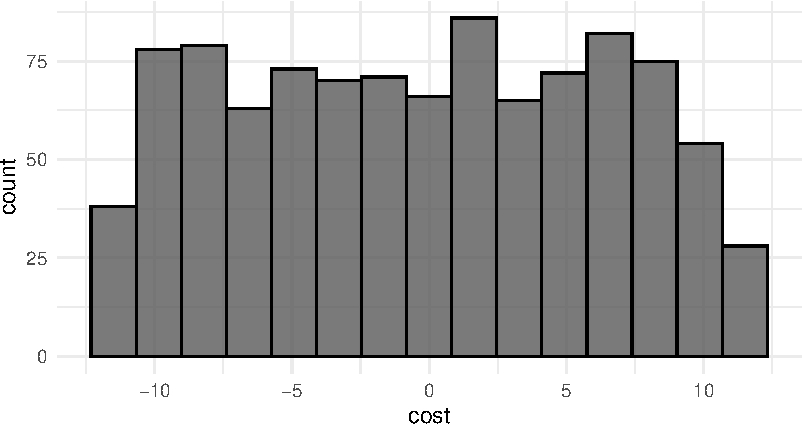
\includegraphics{chapters/chapter4/hyperparameter_optimization_files/figure-pdf/fig-logscale-1.pdf}

}

}

\subcaption{\label{fig-logscale-1}Linear scale sampled by the tuner.}
\end{minipage}%
%
\begin{minipage}[t]{0.50\linewidth}

{\centering 

\raisebox{-\height}{

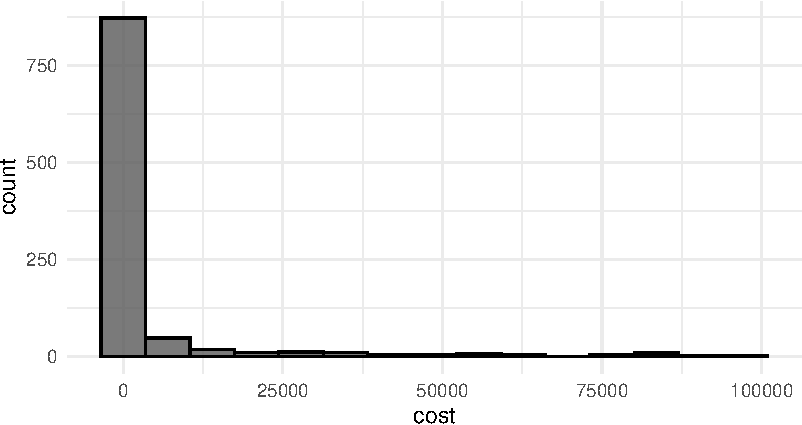
\includegraphics{chapters/chapter4/hyperparameter_optimization_files/figure-pdf/fig-logscale-2.pdf}

}

}

\subcaption{\label{fig-logscale-2}Logarithmic scale seen by the
learner.}
\end{minipage}%

\caption{\label{fig-logscale}Histograms of uniformly sampled values from
the interval \([\log(1e-5), \log(1e5)]\) before (left) and after (right)
exponentiation.}

\end{figure}

To add this transformation to a hyperparameter we simply pass
\texttt{logscale\ =\ TRUE} to
\href{https://paradox.mlr-org.com/reference/to_tune.html}{\texttt{to\_tune()}}.

\begin{Shaded}
\begin{Highlighting}[]
\NormalTok{learner }\OtherTok{=} \FunctionTok{lrn}\NormalTok{(}\StringTok{"classif.svm"}\NormalTok{,}
  \AttributeTok{cost  =} \FunctionTok{to\_tune}\NormalTok{(}\FloatTok{1e{-}5}\NormalTok{, }\FloatTok{1e5}\NormalTok{, }\AttributeTok{logscale =} \ConstantTok{TRUE}\NormalTok{),}
  \AttributeTok{gamma =} \FunctionTok{to\_tune}\NormalTok{(}\FloatTok{1e{-}5}\NormalTok{, }\FloatTok{1e5}\NormalTok{, }\AttributeTok{logscale =} \ConstantTok{TRUE}\NormalTok{),}
  \AttributeTok{kernel =} \StringTok{"radial"}\NormalTok{,}
  \AttributeTok{type =} \StringTok{"C{-}classification"}
\NormalTok{)}

\NormalTok{instance }\OtherTok{=} \FunctionTok{ti}\NormalTok{(}
  \AttributeTok{task =}\NormalTok{ tsk\_sonar,}
  \AttributeTok{learner =}\NormalTok{ learner,}
  \AttributeTok{resampling =} \FunctionTok{rsmp}\NormalTok{(}\StringTok{"cv"}\NormalTok{, }\AttributeTok{folds =} \DecValTok{3}\NormalTok{),}
  \AttributeTok{measures =} \FunctionTok{msr}\NormalTok{(}\StringTok{"classif.ce"}\NormalTok{),}
  \AttributeTok{terminator =} \FunctionTok{trm}\NormalTok{(}\StringTok{"none"}\NormalTok{)}
\NormalTok{)}

\NormalTok{tuner}\SpecialCharTok{$}\FunctionTok{optimize}\NormalTok{(instance)}
\end{Highlighting}
\end{Shaded}

\begin{verbatim}
    cost  gamma learner_param_vals  x_domain classif.ce
1: 5.756 -5.756          <list[4]> <list[2]>     0.1394
\end{verbatim}

We can see from this example that using the log transformation improved
the hyperparameter search, as \texttt{classif.ce} is smaller.

Note that the fields \texttt{cost} and \texttt{gamma} show the optimal
values \emph{before} transformation, whereas \texttt{x\_domain} and
\texttt{learner\_param\_vals} contain optimal values \emph{after}
transformation, it is these latter fields you would take forward for
future model use.

\begin{Shaded}
\begin{Highlighting}[]
\NormalTok{instance}\SpecialCharTok{$}\NormalTok{result}\SpecialCharTok{$}\NormalTok{x\_domain}
\end{Highlighting}
\end{Shaded}

\begin{verbatim}
[[1]]
[[1]]$cost
[1] 316.2

[[1]]$gamma
[1] 0.003162
\end{verbatim}

In Section~\ref{sec-defining-search-spaces} we will look at how to
implement more complex, custom transformations for any hyperparameter or
combination of hyperparameters. Now we will look at how to put
everything into practice so we can make use of the tuned model (and the
transformed hyperparameters).

\hypertarget{sec-analyzing-result}{%
\subsection{Analyzing and Using the Result}\label{sec-analyzing-result}}

Independently of whether you use
\href{https://mlr3tuning.mlr-org.com/reference/ti.html}{\texttt{ti()}}
or
\href{https://mlr3tuning.mlr-org.com/reference/tune.html}{\texttt{tune()}},
or if you include transformations or not, the created objects and the
output are structurally the same and the instance's archive lists all
evaluated hyperparameter configurations:

\begin{Shaded}
\begin{Highlighting}[]
\FunctionTok{as.data.table}\NormalTok{(instance}\SpecialCharTok{$}\NormalTok{archive)[}\DecValTok{1}\SpecialCharTok{:}\DecValTok{3}\NormalTok{, .(cost, gamma, classif.ce)]}
\end{Highlighting}
\end{Shaded}

\begin{verbatim}
      cost   gamma classif.ce
1: -11.513  -5.756     0.4665
2:  -5.756 -11.513     0.4665
3:  -5.756  11.513     0.4665
\end{verbatim}

Each row of the archive is a different evaluated configuration. The
columns show the tested configurations (before transformation) and the
chosen performance measure. We can also manually inspect the archive to
determine other important features such as time of evaluation, model
runtime, and any errors or warnings that occurred during tuning.

\begin{Shaded}
\begin{Highlighting}[]
\FunctionTok{as.data.table}\NormalTok{(instance}\SpecialCharTok{$}\NormalTok{archive)[}\DecValTok{1}\SpecialCharTok{:}\DecValTok{3}\NormalTok{,}
\NormalTok{  .(timestamp, runtime\_learners, errors, warnings)]}
\end{Highlighting}
\end{Shaded}

\begin{verbatim}
             timestamp runtime_learners errors warnings
1: 2023-07-04 15:21:47            0.031      0        0
2: 2023-07-04 15:21:47            0.028      0        0
3: 2023-07-04 15:21:47            0.031      0        0
\end{verbatim}

Another powerful feature of the instance is that we can score the
internal
\href{https://mlr3.mlr-org.com/reference/ResampleResult.html}{\texttt{ResampleResult}}s
on a different performance measure, for example looking at false
negative rate and false positive rate as well as classification error:

\begin{Shaded}
\begin{Highlighting}[]
\FunctionTok{as.data.table}\NormalTok{(instance}\SpecialCharTok{$}\NormalTok{archive,}
  \AttributeTok{measures =} \FunctionTok{msrs}\NormalTok{(}\FunctionTok{c}\NormalTok{(}\StringTok{"classif.fpr"}\NormalTok{, }\StringTok{"classif.fnr"}\NormalTok{)))[}\DecValTok{1}\SpecialCharTok{:}\DecValTok{5}\NormalTok{ ,}
\NormalTok{  .(cost, gamma, classif.ce, classif.fpr, classif.fnr)]}
\end{Highlighting}
\end{Shaded}

\begin{verbatim}
      cost   gamma classif.ce classif.fpr classif.fnr
1: -11.513  -5.756     0.4665      1.0000     0.00000
2:  -5.756 -11.513     0.4665      1.0000     0.00000
3:  -5.756  11.513     0.4665      1.0000     0.00000
4:   0.000  -5.756     0.2308      0.3186     0.14997
5:   5.756  -5.756     0.1394      0.2089     0.08056
\end{verbatim}

You can access all the resamplings combined in a
\href{https://mlr3.mlr-org.com/reference/BenchmarkResult.html}{\texttt{BenchmarkResult}}
object with \texttt{instance\$archive\$benchmark\_result}.

Finally, to visualize the results, you can use
\href{https://mlr3viz.mlr-org.com/reference/autoplot.TuningInstanceSingleCrit.html}{\texttt{autoplot.TuningInstanceSingleCrit}}
(Figure~\ref{fig-surface}). In this example we can observe one of the
flaws (by design) in grid search, despite testing 25 configurations, we
only saw five unique values for each hyperparameter.

\begin{Shaded}
\begin{Highlighting}[]
\FunctionTok{autoplot}\NormalTok{(instance, }\AttributeTok{type =} \StringTok{"surface"}\NormalTok{)}
\end{Highlighting}
\end{Shaded}

\begin{figure}[H]

{\centering 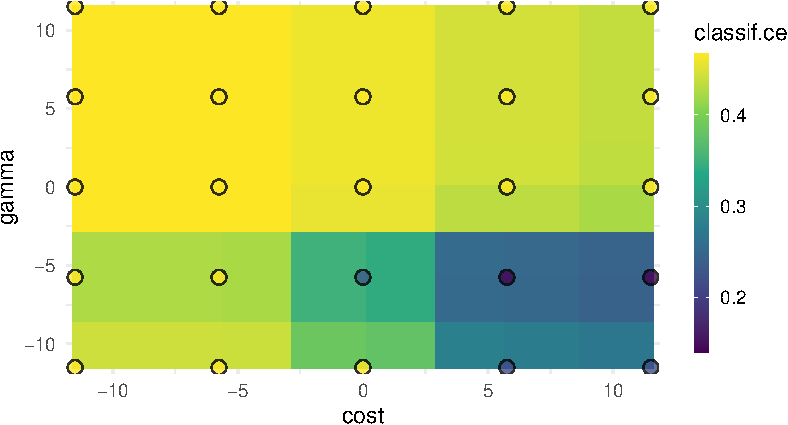
\includegraphics[width=1\textwidth,height=\textheight]{chapters/chapter4/hyperparameter_optimization_files/figure-pdf/fig-surface-1.pdf}

}

\caption{\label{fig-surface}Model performance with different
configurations for \texttt{cost} and \texttt{gamma}. Bright yellow
regions represent the model performing worse and dark blue performing
better. We can see that high \texttt{cost} values and low \texttt{gamma}
values achieve the best performance. Note that we should not directly
infer the performance of new unseen values from the heatmap since it is
only an interpolation based on a surrogate model (\texttt{regr.ranger}).
However, we can see the general interaction between the
hyperparameters.}

\end{figure}

\hypertarget{training-an-optimized-model}{%
\subsubsection*{Training an optimized
model}\label{training-an-optimized-model}}

Once we found good hyperparameters for our learner through tuning, we
can use them to train a final model on the whole data. To do this we
simply construct a new learner with the same underlying algorithm and
set the learner hyperparameters to the optimal configuration:

\begin{Shaded}
\begin{Highlighting}[]
\NormalTok{lrn\_svm\_tuned }\OtherTok{=} \FunctionTok{lrn}\NormalTok{(}\StringTok{"classif.svm"}\NormalTok{)}
\NormalTok{lrn\_svm\_tuned}\SpecialCharTok{$}\NormalTok{param\_set}\SpecialCharTok{$}\NormalTok{values }\OtherTok{=}\NormalTok{ instance}\SpecialCharTok{$}\NormalTok{result\_learner\_param\_vals}
\end{Highlighting}
\end{Shaded}

Now we can train the learner on the full dataset and we are ready to
make predictions.

\begin{Shaded}
\begin{Highlighting}[]
\NormalTok{lrn\_svm\_tuned}\SpecialCharTok{$}\FunctionTok{train}\NormalTok{(tsk\_sonar)}\SpecialCharTok{$}\NormalTok{model}
\end{Highlighting}
\end{Shaded}

\begin{verbatim}

Call:
svm.default(x = data, y = task$truth(), type = "C-classification", 
    kernel = "radial", gamma = 0.00316227766016838, cost = 316.227766016838, 
    probability = (self$predict_type == "prob"))


Parameters:
   SVM-Type:  C-classification 
 SVM-Kernel:  radial 
       cost:  316.2 

Number of Support Vectors:  93
\end{verbatim}

\hypertarget{sec-autotuner}{%
\section{\texorpdfstring{Convenient Tuning with \texttt{tune} and
\texttt{auto\_tuner}}{Convenient Tuning with tune and auto\_tuner}}\label{sec-autotuner}}

In the previous section, we looked at constructing and manually putting
together the components of HPO by creating a tuning instance using
\href{https://mlr3tuning.mlr-org.com/reference/ti.html}{\texttt{ti()}},
passing this to the tuner, and then calling \texttt{\$optimize()} to
start the tuning process. \texttt{mlr3tuning} includes two helper
methods to simplify this process further.

The first helper function is
\href{https://mlr3tuning.mlr-org.com/reference/tune.html}{\texttt{tune()}},
which creates the tuning instance and calls \texttt{\$optimize()} for
you. You may prefer the manual method with \texttt{ti()} if you want to
view and make changes to the instance before tuning.

\begin{Shaded}
\begin{Highlighting}[]
\NormalTok{tnr\_grid\_search }\OtherTok{=} \FunctionTok{tnr}\NormalTok{(}\StringTok{"grid\_search"}\NormalTok{, }\AttributeTok{resolution =} \DecValTok{5}\NormalTok{, }\AttributeTok{batch\_size =} \DecValTok{5}\NormalTok{)}
\NormalTok{lrn\_svm }\OtherTok{=} \FunctionTok{lrn}\NormalTok{(}\StringTok{"classif.svm"}\NormalTok{,}
  \AttributeTok{cost  =} \FunctionTok{to\_tune}\NormalTok{(}\FloatTok{1e{-}5}\NormalTok{, }\FloatTok{1e5}\NormalTok{, }\AttributeTok{logscale =} \ConstantTok{TRUE}\NormalTok{),}
  \AttributeTok{gamma =} \FunctionTok{to\_tune}\NormalTok{(}\FloatTok{1e{-}5}\NormalTok{, }\FloatTok{1e5}\NormalTok{, }\AttributeTok{logscale =} \ConstantTok{TRUE}\NormalTok{),}
  \AttributeTok{kernel =} \StringTok{"radial"}\NormalTok{,}
  \AttributeTok{type =} \StringTok{"C{-}classification"}
\NormalTok{)}
\NormalTok{rsmp\_cv3 }\OtherTok{=} \FunctionTok{rsmp}\NormalTok{(}\StringTok{"cv"}\NormalTok{, }\AttributeTok{folds =} \DecValTok{3}\NormalTok{)}
\NormalTok{msr\_ce }\OtherTok{=} \FunctionTok{msr}\NormalTok{(}\StringTok{"classif.ce"}\NormalTok{)}

\NormalTok{instance }\OtherTok{=} \FunctionTok{tune}\NormalTok{(}
  \AttributeTok{tuner =}\NormalTok{ tnr\_grid\_search,}
  \AttributeTok{task =}\NormalTok{ tsk\_sonar,}
  \AttributeTok{learner =}\NormalTok{ lrn\_svm,}
  \AttributeTok{resampling =}\NormalTok{ rsmp\_cv3,}
  \AttributeTok{measures =}\NormalTok{ msr\_ce}
\NormalTok{)}
\NormalTok{instance}\SpecialCharTok{$}\NormalTok{result}
\end{Highlighting}
\end{Shaded}

\begin{verbatim}
    cost  gamma learner_param_vals  x_domain classif.ce
1: 5.756 -5.756          <list[4]> <list[2]>     0.1444
\end{verbatim}

The other helper function is
\href{https://mlr3tuning.mlr-org.com/reference/auto_tuner.html}{\texttt{auto\_tuner}},
which creates an object of class
\href{https://mlr3tuning.mlr-org.com/reference/AutoTuner.html}{\texttt{AutoTuner}}\index{\texttt{AutoTuner}}
(Figure~\ref{fig-auto-tuner}). The \texttt{AutoTuner} inherits from the
\href{https://mlr3.mlr-org.com/reference/Learner.html}{\texttt{Learner}}
class and wraps all the information needed for tuning, which means you
can treat a learner waiting to be optimized just like any other learner.
Under the hood, the \texttt{AutoTuner} essentially runs \texttt{tune()}
on the data that is passed to the model when \texttt{\$train()} is
called and then sets the learner parameters to the optimal
configuration.

\begin{Shaded}
\begin{Highlighting}[]
\NormalTok{at }\OtherTok{=} \FunctionTok{auto\_tuner}\NormalTok{(}
  \AttributeTok{tuner =}\NormalTok{ tnr\_grid\_search,}
  \AttributeTok{learner =}\NormalTok{ lrn\_svm,}
  \AttributeTok{resampling =}\NormalTok{ rsmp\_cv3,}
  \AttributeTok{measure =}\NormalTok{ msr\_ce}
\NormalTok{)}

\NormalTok{at}
\end{Highlighting}
\end{Shaded}

\begin{verbatim}
<AutoTuner:classif.svm.tuned>
* Model: list
* Search Space:
<ParamSet>
      id    class  lower upper nlevels        default value
1:  cost ParamDbl -11.51 11.51     Inf <NoDefault[3]>      
2: gamma ParamDbl -11.51 11.51     Inf <NoDefault[3]>      
Trafo is set.
* Packages: mlr3, mlr3tuning, mlr3learners, e1071
* Predict Type: response
* Feature Types: logical, integer, numeric
* Properties: multiclass, twoclass
\end{verbatim}

\begin{figure}

{\centering 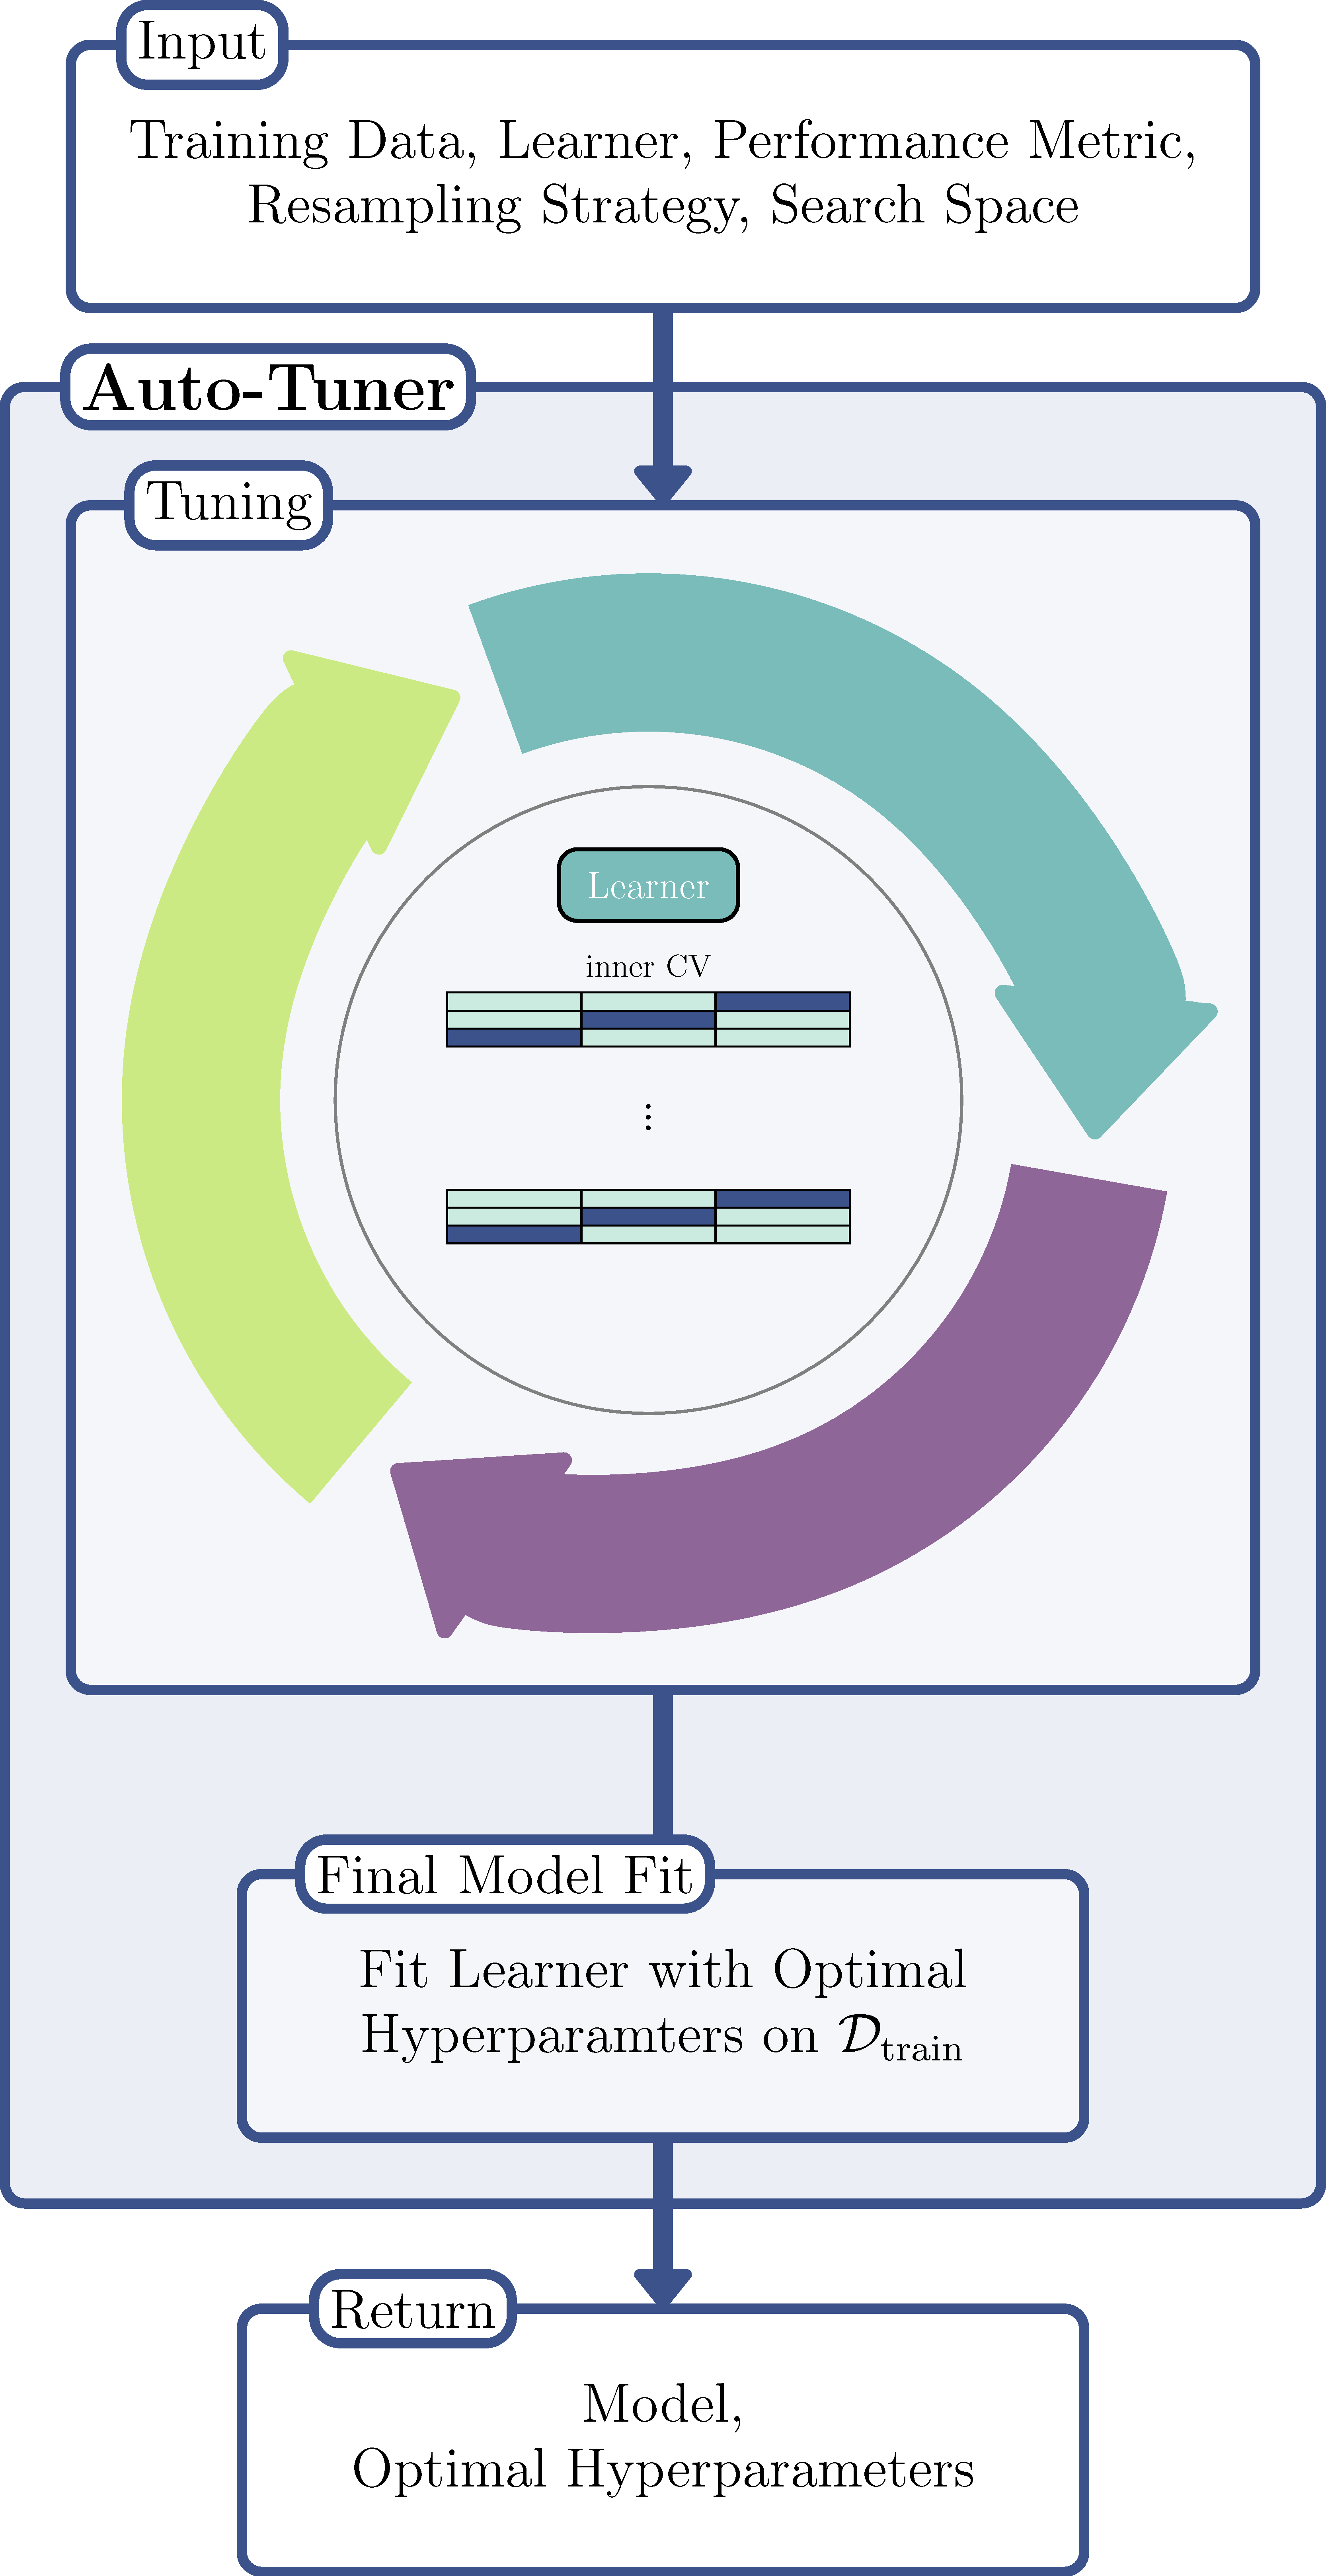
\includegraphics[width=0.6\textwidth]{chapters/chapter4/Figures/mlr3book_figures-12.png}

}

\caption{\label{fig-auto-tuner}Illustration of an Auto-Tuner.}

\end{figure}

And we can now call \texttt{\$train()}, which will first tune the
hyperparameters in the search space listed above before fitting the
optimal model.

\begin{Shaded}
\begin{Highlighting}[]
\NormalTok{split }\OtherTok{=} \FunctionTok{partition}\NormalTok{(tsk\_sonar)}
\NormalTok{at}\SpecialCharTok{$}\FunctionTok{train}\NormalTok{(tsk\_sonar, }\AttributeTok{row\_ids =}\NormalTok{ split}\SpecialCharTok{$}\NormalTok{train)}
\NormalTok{at}\SpecialCharTok{$}\FunctionTok{predict}\NormalTok{(tsk\_sonar, }\AttributeTok{row\_ids =}\NormalTok{ split}\SpecialCharTok{$}\NormalTok{test)}\SpecialCharTok{$}\FunctionTok{score}\NormalTok{()}
\end{Highlighting}
\end{Shaded}

\begin{verbatim}
classif.ce 
    0.2029 
\end{verbatim}

The \texttt{AutoTuner} contains a tuning instance that can be analyzed
like any other instance.

\begin{Shaded}
\begin{Highlighting}[]
\NormalTok{at}\SpecialCharTok{$}\NormalTok{tuning\_instance}\SpecialCharTok{$}\NormalTok{result}
\end{Highlighting}
\end{Shaded}

\begin{verbatim}
    cost  gamma learner_param_vals  x_domain classif.ce
1: 5.756 -5.756          <list[4]> <list[2]>     0.1727
\end{verbatim}

We could also pass the \texttt{AutoTuner} to
\href{https://mlr3.mlr-org.com/reference/resample.html}{\texttt{resample()}}
and
\href{https://mlr3.mlr-org.com/reference/benchmark.html}{\texttt{benchmark()}},
which would result in a nested resampling, discussed next.

\hypertarget{sec-nested-resampling}{%
\section{Nested Resampling}\label{sec-nested-resampling}}

HPO requires additional resampling to reduce bias when estimating the
performance of a model. If the same data is used for determining the
optimal configuration and the evaluation of the resulting model itself,
the actual performance estimate might be biased (Simon 2007). This is
analogous to optimism of the training
error\index{optimism of the training error} described in James et al.
(2014), which occurs when training error is taken as an estimate of
out-of-sample performance.

Nested resampling\index{nested resampling} separates model optimization
from the process of estimating the performance of the tuned model by
adding an additional resampling, i.e., while model performance is
estimated using a resampling method in the `usual way', tuning is then
performed by resampling the resampled data
(Figure~\ref{fig-nested-resampling}). For more details and a formal
introduction to nested resampling the reader is referred to Bischl et
al. (2023) and Simon (2007).

\begin{figure}

{\centering 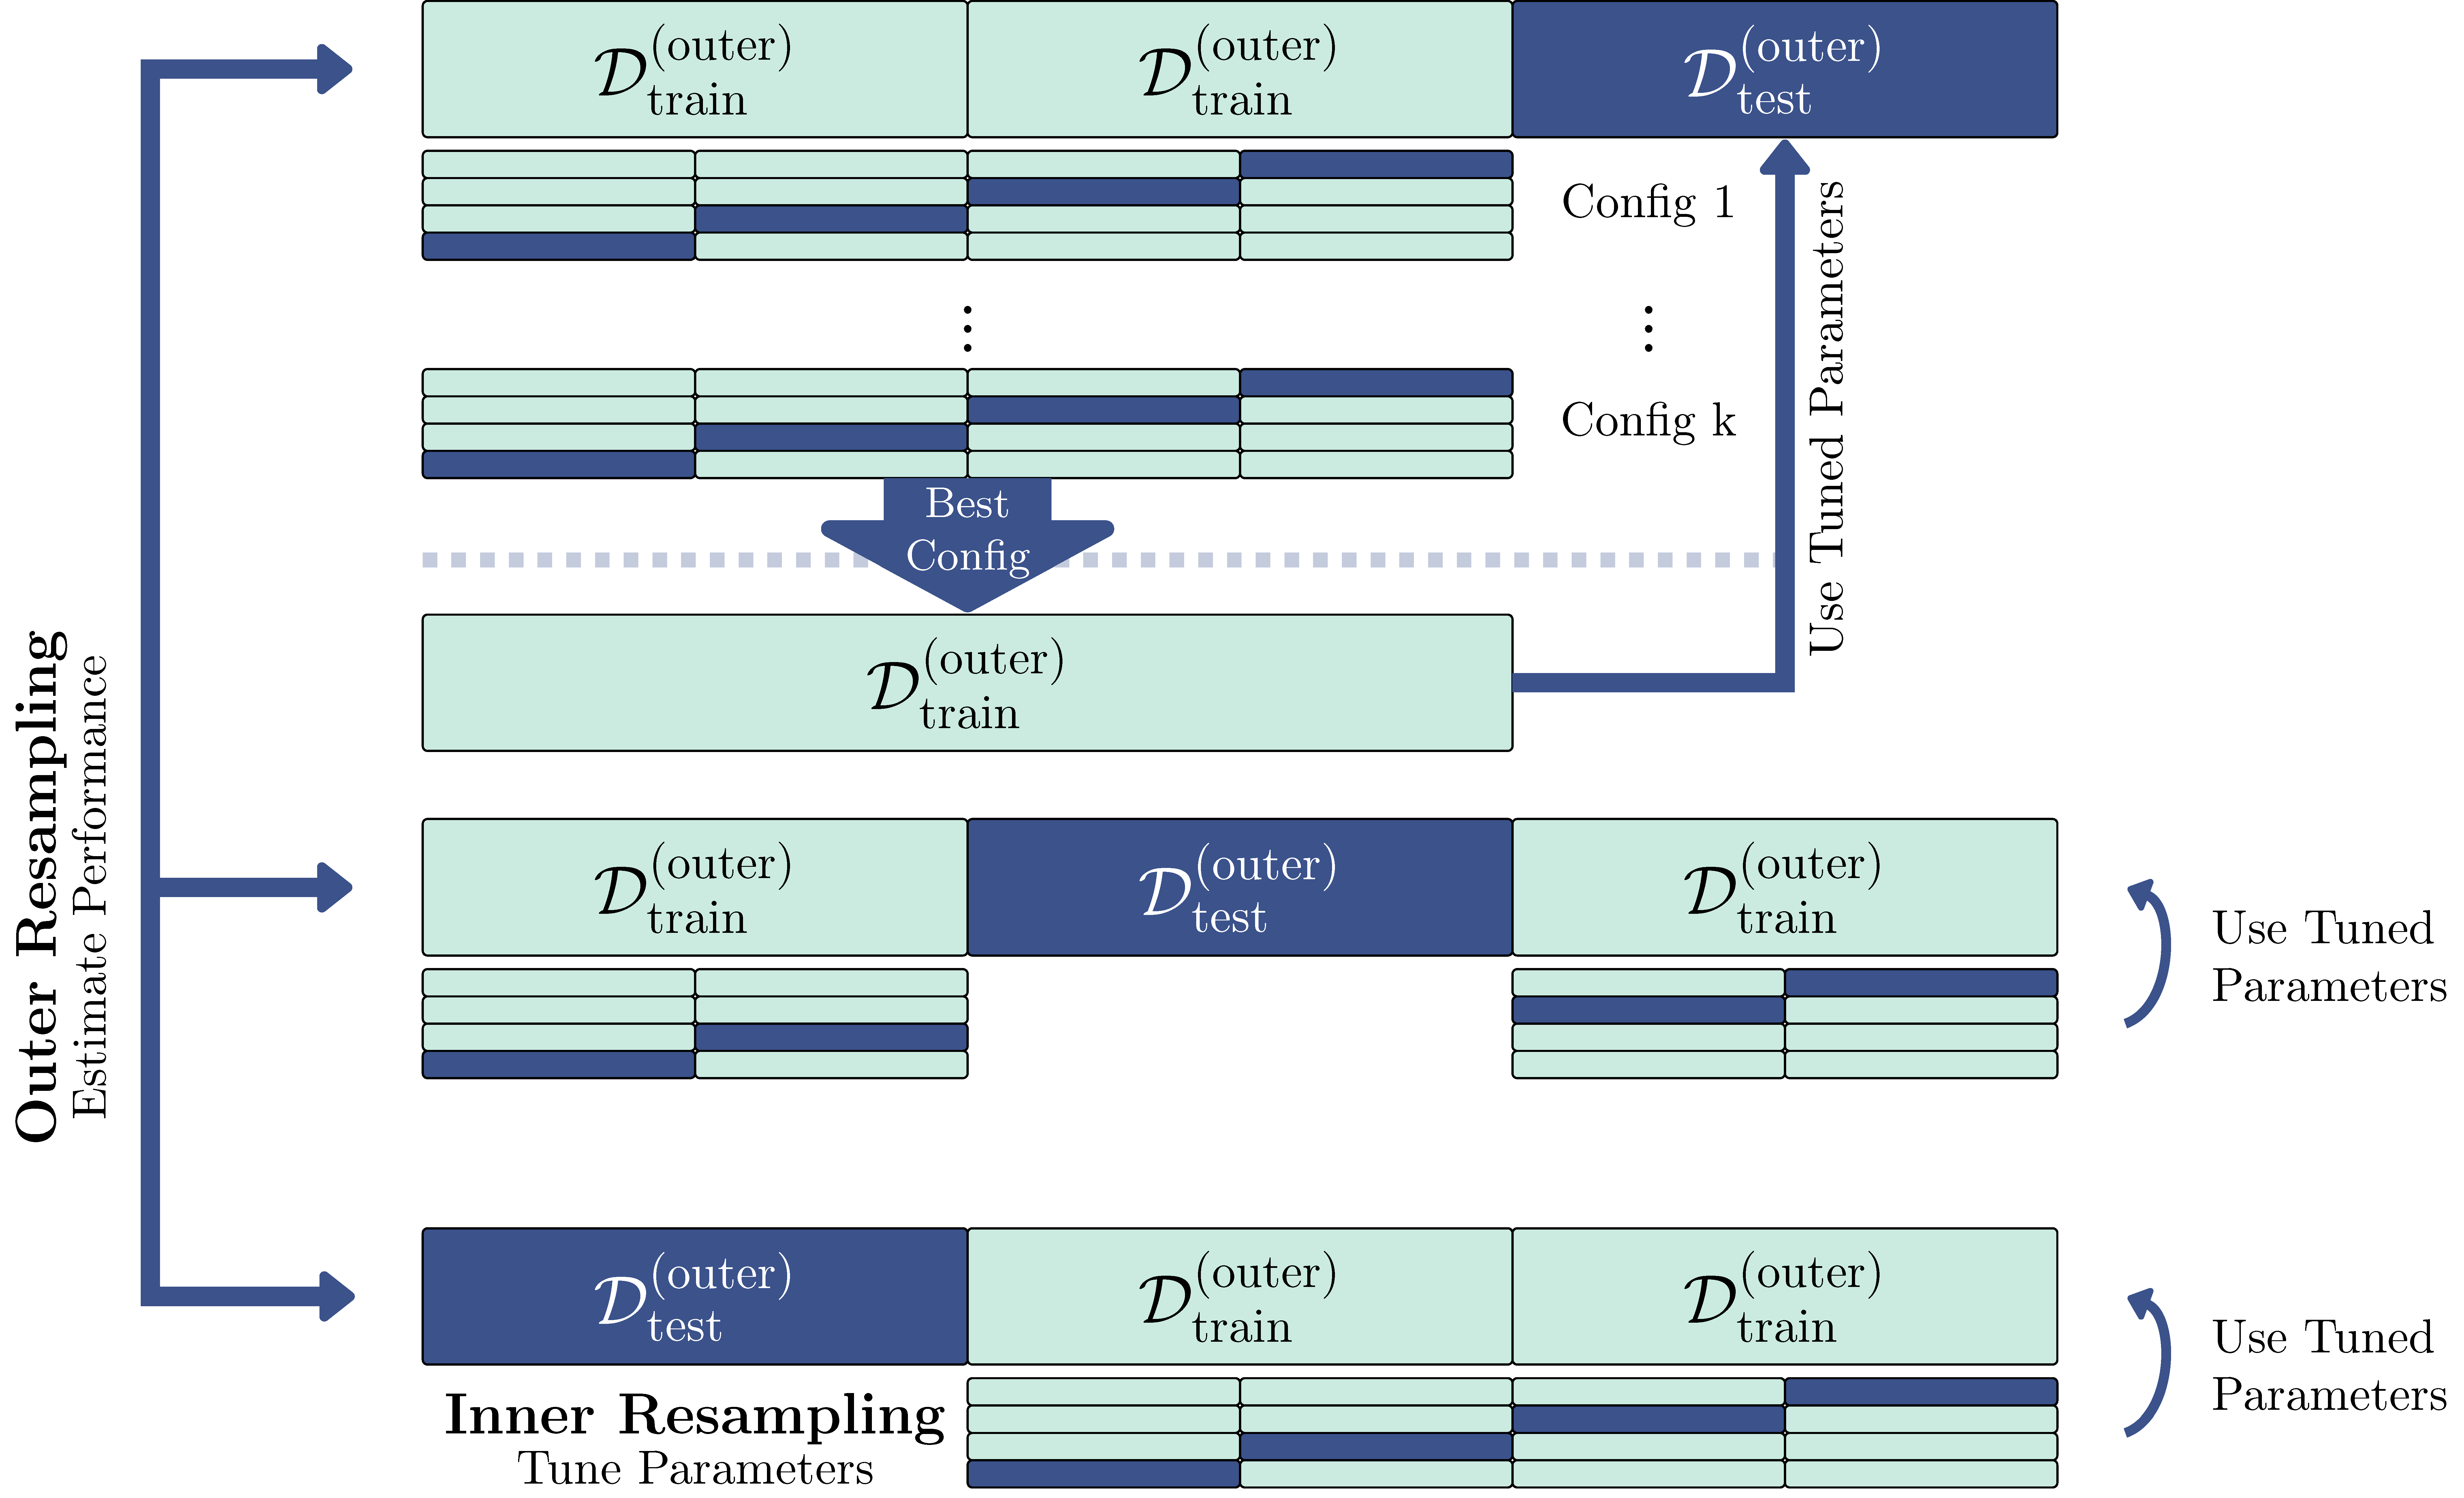
\includegraphics[width=0.8\textwidth,height=\textheight]{chapters/chapter4/Figures/mlr3book_figures-11.png}

}

\caption{\label{fig-nested-resampling}An illustration of nested
resampling. The large blocks represent three-fold CV for the outer
resampling for model evaluation and the small blocks represent four-fold
CV for the inner resampling for HPO. The light blue blocks are the
training sets and the dark blue blocks are the test sets.}

\end{figure}

Figure~\ref{fig-nested-resampling} represents the following example of
nested resampling:

\begin{enumerate}
\def\labelenumi{\arabic{enumi}.}
\tightlist
\item
  Outer resampling start -- Instantiate three-fold CV to create
  different testing and training datasets.
\item
  Inner resampling -- Within the outer training data instantiate
  four-fold CV to create different inner testing and training datasets.
\item
  HPO -- Tune the hyperparameters on the outer training set (large,
  light blue blocks) using the inner data splits.
\item
  Training -- Fit the learner on the outer training dataset using the
  optimal hyperparameter configuration obtained from the inner
  resampling (small blocks).
\item
  Evaluation -- Evaluate the performance of the learner on the outer
  testing data (large, dark blue block).
\item
  Outer resampling repeats -- Repeat (2)-(5) for each of the three outer
  folds.
\item
  Aggregation -- Take the sample mean of the three performance values
  for an unbiased performance estimate.
\end{enumerate}

The inner resampling produces generalization performance estimates for
each configuration and selects the optimal configuration to be evaluated
on the outer resampling. The outer resampling then produces
generalization estimates for these optimal configurations. The result
from the outer resampling can be used for comparison to other models
trained and tested on the same outer folds.

\begin{tcolorbox}[enhanced jigsaw, opacitybacktitle=0.6, rightrule=.15mm, opacityback=0, arc=.35mm, breakable, titlerule=0mm, colframe=quarto-callout-tip-color-frame, coltitle=black, bottomrule=.15mm, toprule=.15mm, colback=white, colbacktitle=quarto-callout-tip-color!10!white, bottomtitle=1mm, toptitle=1mm, title=\textcolor{quarto-callout-tip-color}{\faLightbulb}\hspace{0.5em}{Nested Resampling and Parallelization}, leftrule=.75mm, left=2mm]

Nested resampling is computationally expensive, three outer folds and
four inner folds with a grid search of resolution five used to tune two
parameters, results in \(3*4*5^2 = 300\) iterations of model
training/testing. If you have the resources we recommend utilizing
parallelization when tuning (Section~\ref{sec-parallelization}).

\end{tcolorbox}

A common mistake is to think of nested resampling as a method to select
optimal model configurations. Nested resampling is a method to compare
models and to estimate the generalization performance of a tuned model,
however, this is the performance based on multiple different
configurations (one from each outer fold) and not performance based on a
\emph{single} configuration (Section~\ref{sec-resample-overfitting}). If
you are interested in identifying optimal configurations, then use
\href{https://mlr3tuning.mlr-org.com/reference/tune.html}{\texttt{tune()}}\index{\texttt{tune()}}/\href{https://mlr3tuning.mlr-org.com/reference/ti.html}{\texttt{ti()}}
or
\href{https://mlr3tuning.mlr-org.com/reference/auto_tuner.html}{\texttt{auto\_tuner()}}\index{\texttt{auto\_tuner()}}
with \texttt{\$train()} on the complete dataset.

\hypertarget{nested-resampling-with-an-autotuner}{%
\subsection{\texorpdfstring{Nested Resampling with an
\texttt{AutoTuner}}{Nested Resampling with an AutoTuner}}\label{nested-resampling-with-an-autotuner}}

While the theory of nested resampling may seem complicated, it is all
automated in \texttt{mlr3tuning} by simply passing an \texttt{AutoTuner}
to
\href{https://mlr3.mlr-org.com/reference/resample.html}{\texttt{resample()}}
or
\href{https://mlr3.mlr-org.com/reference/benchmark.html}{\texttt{benchmark()}}.
Continuing with our previous example, we will use the auto-tuner to
resample a support vector classifier with three-fold CV in the outer
resampling and four-fold CV in the inner resampling.

\begin{Shaded}
\begin{Highlighting}[]
\NormalTok{at }\OtherTok{=} \FunctionTok{auto\_tuner}\NormalTok{(}
  \AttributeTok{tuner =}\NormalTok{ tnr\_grid\_search,}
  \AttributeTok{learner =}\NormalTok{ lrn\_svm,}
  \AttributeTok{resampling =} \FunctionTok{rsmp}\NormalTok{(}\StringTok{"cv"}\NormalTok{, }\AttributeTok{folds =} \DecValTok{4}\NormalTok{),}
  \AttributeTok{measure =}\NormalTok{ msr\_ce,}
\NormalTok{)}

\NormalTok{rr }\OtherTok{=} \FunctionTok{resample}\NormalTok{(tsk\_sonar, at, rsmp\_cv3, }\AttributeTok{store\_models =} \ConstantTok{TRUE}\NormalTok{)}

\NormalTok{rr}
\end{Highlighting}
\end{Shaded}

\begin{verbatim}
<ResampleResult> with 3 resampling iterations
 task_id        learner_id resampling_id iteration warnings errors
   sonar classif.svm.tuned            cv         1        0      0
   sonar classif.svm.tuned            cv         2        0      0
   sonar classif.svm.tuned            cv         3        0      0
\end{verbatim}

Note that we set \texttt{store\_models\ =\ TRUE} so that the
\texttt{AutoTuner} models (fitted on the outer training data) are
stored, which also enables investigation of the inner tuning instances.
While we used k-fold CV for both the inner and outer resampling
strategy, you could use different resampling strategies
(Section~\ref{sec-resampling}) and also different parallelization
methods (Section~\ref{sec-nested-resampling-parallelization}).

The estimated performance of a tuned model is reported as the aggregated
performance of all outer resampling iterations, which is a less biased
estimate of future model performance.

\begin{Shaded}
\begin{Highlighting}[]
\NormalTok{rr}\SpecialCharTok{$}\FunctionTok{aggregate}\NormalTok{()}
\end{Highlighting}
\end{Shaded}

\begin{verbatim}
classif.ce 
    0.1589 
\end{verbatim}

In addition to the methods described in Section~\ref{sec-resampling},
\href{https://mlr3tuning.mlr-org.com/reference/extract_inner_tuning_results.html}{\texttt{extract\_inner\_tuning\_results()}}
and
\href{https://mlr3tuning.mlr-org.com/reference/extract_inner_tuning_archives.html}{\texttt{extract\_inner\_tuning\_archives()}}
return the optimal configurations (across all outer folds) and full
tuning archives, respectively.

\begin{Shaded}
\begin{Highlighting}[]
\FunctionTok{extract\_inner\_tuning\_results}\NormalTok{(rr)[,}
\NormalTok{  .(iteration, cost, gamma, classif.ce)]}
\end{Highlighting}
\end{Shaded}

\begin{verbatim}
   iteration  cost  gamma classif.ce
1:         1 11.51 -5.756     0.2174
2:         2 11.51 -5.756     0.2086
3:         3 11.51 -5.756     0.1796
\end{verbatim}

\begin{Shaded}
\begin{Highlighting}[]
\FunctionTok{extract\_inner\_tuning\_archives}\NormalTok{(rr)[}\DecValTok{1}\SpecialCharTok{:}\DecValTok{3}\NormalTok{,}
\NormalTok{  .(iteration, cost, gamma, classif.ce)]}
\end{Highlighting}
\end{Shaded}

\begin{verbatim}
   iteration   cost   gamma classif.ce
1:         1 -11.51 -11.513     0.5286
2:         1 -11.51  11.513     0.5286
3:         1   0.00  -5.756     0.2981
\end{verbatim}

\hypertarget{sec-resample-overfitting}{%
\subsection{The Right (and Wrong) Way to Estimate
Performance}\label{sec-resample-overfitting}}

\begin{tcolorbox}[enhanced jigsaw, colframe=quarto-callout-note-color-frame, rightrule=.15mm, bottomrule=.15mm, toprule=.15mm, opacityback=0, colback=white, left=2mm, arc=.35mm, breakable, leftrule=.75mm]
\begin{minipage}[t]{5.5mm}
\textcolor{quarto-callout-note-color}{\faInfo}
\end{minipage}%
\begin{minipage}[t]{\textwidth - 5.5mm}

\textbf{This section covers advanced ML or technical
details.}\vspace{2mm}

\end{minipage}%
\end{tcolorbox}

In this short section we will empirically demonstrate that directly
reporting tuning performance without nested resampling results in
optimistically biased performance estimates. In this experiment we tune
several parameters from \texttt{lrn("classif.xgboost")}. To best
estimate the generalization performance we make use of the
\texttt{"moons"}
\href{https://mlr3.mlr-org.com/reference/TaskGenerator.html}{\texttt{TaskGenerator}}\index{\texttt{TaskGenerator}}{\marginnote{\begin{footnotesize}\texttt{TaskGenerator}\end{footnotesize}}}.
The \texttt{TaskGenerator} class is used when you want to simulate data
for use in experiments, these are very useful in cases such as this
experiment when you need access to an infinite number of data points to
estimate quantities such as the generalization error.

We begin by loading our learner, task generator, and generating 100
training data points and 1,000,000 testing data points.

\begin{Shaded}
\begin{Highlighting}[]
\NormalTok{lrn\_xgboost }\OtherTok{=} \FunctionTok{lrn}\NormalTok{(}\StringTok{"classif.xgboost"}\NormalTok{,}
  \AttributeTok{eta               =} \FunctionTok{to\_tune}\NormalTok{(}\FloatTok{1e{-}4}\NormalTok{, }\DecValTok{1}\NormalTok{, }\AttributeTok{logscale =} \ConstantTok{TRUE}\NormalTok{),}
  \AttributeTok{max\_depth         =} \FunctionTok{to\_tune}\NormalTok{(}\DecValTok{1}\NormalTok{, }\DecValTok{20}\NormalTok{),}
  \AttributeTok{colsample\_bytree  =} \FunctionTok{to\_tune}\NormalTok{(}\FloatTok{1e{-}1}\NormalTok{, }\DecValTok{1}\NormalTok{),}
  \AttributeTok{colsample\_bylevel =} \FunctionTok{to\_tune}\NormalTok{(}\FloatTok{1e{-}1}\NormalTok{, }\DecValTok{1}\NormalTok{),}
  \AttributeTok{lambda            =} \FunctionTok{to\_tune}\NormalTok{(}\FloatTok{1e{-}3}\NormalTok{, }\FloatTok{1e3}\NormalTok{, }\AttributeTok{logscale =} \ConstantTok{TRUE}\NormalTok{),}
  \AttributeTok{alpha             =} \FunctionTok{to\_tune}\NormalTok{(}\FloatTok{1e{-}3}\NormalTok{, }\FloatTok{1e3}\NormalTok{, }\AttributeTok{logscale =} \ConstantTok{TRUE}\NormalTok{),}
  \AttributeTok{subsample         =} \FunctionTok{to\_tune}\NormalTok{(}\FloatTok{1e{-}1}\NormalTok{, }\DecValTok{1}\NormalTok{)}
\NormalTok{)}
\NormalTok{tsk\_moons }\OtherTok{=} \FunctionTok{tgen}\NormalTok{(}\StringTok{"moons"}\NormalTok{)}
\NormalTok{tsk\_moons\_train }\OtherTok{=}\NormalTok{ tsk\_moons}\SpecialCharTok{$}\FunctionTok{generate}\NormalTok{(}\DecValTok{100}\NormalTok{)}
\NormalTok{tsk\_moons\_test }\OtherTok{=}\NormalTok{ tsk\_moons}\SpecialCharTok{$}\FunctionTok{generate}\NormalTok{(}\DecValTok{1000000}\NormalTok{)}
\end{Highlighting}
\end{Shaded}

Now we will tune the learner with respect to the classification error,
using holdout resampling and random search with 700 evaluations. We then
report the tuning performance without nested resampling.

\begin{Shaded}
\begin{Highlighting}[]
\NormalTok{tnr\_random }\OtherTok{=} \FunctionTok{tnr}\NormalTok{(}\StringTok{"random\_search"}\NormalTok{)}
\NormalTok{rsmp\_holdout }\OtherTok{=} \FunctionTok{rsmp}\NormalTok{(}\StringTok{"holdout"}\NormalTok{)}
\NormalTok{trm\_evals700 }\OtherTok{=} \FunctionTok{trm}\NormalTok{(}\StringTok{"evals"}\NormalTok{, }\AttributeTok{n\_evals =} \DecValTok{700}\NormalTok{)}

\NormalTok{instance }\OtherTok{=} \FunctionTok{tune}\NormalTok{(}
  \AttributeTok{tuner =}\NormalTok{ tnr\_random,}
  \AttributeTok{task =}\NormalTok{ tsk\_moons\_train,}
  \AttributeTok{learner =}\NormalTok{ lrn\_xgboost,}
  \AttributeTok{resampling =}\NormalTok{ rsmp\_holdout,}
  \AttributeTok{measures =}\NormalTok{ msr\_ce,}
  \AttributeTok{terminator =}\NormalTok{ trm\_evals700}
\NormalTok{)}

\NormalTok{insample }\OtherTok{=}\NormalTok{ instance}\SpecialCharTok{$}\NormalTok{result\_y}
\end{Highlighting}
\end{Shaded}

Next, we estimate generalization error by nested resampling (below we
use an outer five-fold CV), using an \texttt{AutoTuner}:

\begin{Shaded}
\begin{Highlighting}[]
\CommentTok{\# same setup as above}
\NormalTok{at }\OtherTok{=} \FunctionTok{auto\_tuner}\NormalTok{(}
  \AttributeTok{tuner =}\NormalTok{ tnr\_random,}
  \AttributeTok{learner =}\NormalTok{ lrn\_xgboost,}
  \AttributeTok{resampling =}\NormalTok{ rsmp\_holdout,}
  \AttributeTok{measure =}\NormalTok{ msr\_ce,}
  \AttributeTok{terminator =}\NormalTok{ trm\_evals700}
\NormalTok{)}

\NormalTok{rsmp\_cv5 }\OtherTok{=} \FunctionTok{rsmp}\NormalTok{(}\StringTok{"cv"}\NormalTok{, }\AttributeTok{folds =} \DecValTok{5}\NormalTok{)}

\NormalTok{outsample }\OtherTok{=} \FunctionTok{resample}\NormalTok{(tsk\_moons\_train, at, rsmp\_cv5)}\SpecialCharTok{$}\FunctionTok{aggregate}\NormalTok{()}
\end{Highlighting}
\end{Shaded}

And finally, we estimate the generalization
error\index{generalization error} by training the tuned learner (i.e.,
using the values from the \texttt{instance} above) on the full training
data again and predicting on the test data.

\begin{Shaded}
\begin{Highlighting}[]
\NormalTok{lrn\_xgboost\_tuned }\OtherTok{=} \FunctionTok{lrn}\NormalTok{(}\StringTok{"classif.xgboost"}\NormalTok{)}
\NormalTok{lrn\_xgboost\_tuned}\SpecialCharTok{$}\NormalTok{param\_set}\SpecialCharTok{$}\FunctionTok{set\_values}\NormalTok{(}
  \AttributeTok{.values =}\NormalTok{ instance}\SpecialCharTok{$}\NormalTok{result\_learner\_param\_vals)}
\NormalTok{generalization }\OtherTok{=}\NormalTok{ lrn\_xgboost\_tuned}\SpecialCharTok{$}\FunctionTok{train}\NormalTok{(tsk\_moons\_train)}\SpecialCharTok{$}
  \FunctionTok{predict}\NormalTok{(tsk\_moons\_test)}\SpecialCharTok{$}\FunctionTok{score}\NormalTok{()}
\end{Highlighting}
\end{Shaded}

Now we can compare these three values:

\begin{Shaded}
\begin{Highlighting}[]
\FunctionTok{round}\NormalTok{(}\FunctionTok{c}\NormalTok{(}\AttributeTok{true\_generalization =} \FunctionTok{as.numeric}\NormalTok{(generalization),}
  \AttributeTok{without\_nested\_resampling =} \FunctionTok{as.numeric}\NormalTok{(insample),}
  \AttributeTok{with\_nested\_resampling =} \FunctionTok{as.numeric}\NormalTok{(outsample)), }\DecValTok{2}\NormalTok{)}
\end{Highlighting}
\end{Shaded}

\begin{verbatim}
      true_generalization without_nested_resampling 
                     0.19                      0.06 
   with_nested_resampling 
                     0.22 
\end{verbatim}

We find that the performance estimate from unnested tuning
optimistically overestimates the true performance (which could indicate
`meta-overfitting' to the specific inner holdout-splits), while the
outer estimate from nested resampling works much better.

\hypertarget{sec-defining-search-spaces}{%
\section{More Advanced Search Spaces}\label{sec-defining-search-spaces}}

Up until now, we have only considered tuning simple search spaces
limited to a few numeric hyperparameters. In this section, we will first
look at how to tune different scalar parameter classes with
\href{https://paradox.mlr-org.com/reference/to_tune.html}{\texttt{to\_tune()}},
and then how to define your own search space with
\href{https://paradox.mlr-org.com/reference/ParamSet.html}{\texttt{ParamSet}}
to create more advanced search spaces that may include tuning over
vectors, transformations, and handling parameter dependencies. Finally,
we will consider how to access a database of standardized search spaces
from the literature.

\hypertarget{scalar-parameter-tuning}{%
\subsection{Scalar Parameter Tuning}\label{scalar-parameter-tuning}}

The
\href{https://paradox.mlr-org.com/reference/to_tune.html}{\texttt{to\_tune()}}
function can be used to tune parameters of any class, whether they are
scalar or vectors. To best understand this function, we will consider
what is happening behind the scenes. When \texttt{to\_tune()} is used in
a learner, implicitly a
\href{https://paradox.mlr-org.com/reference/ParamSet.html}{\texttt{ParamSet}}
is created just for the tuning search space:

\begin{Shaded}
\begin{Highlighting}[]
\NormalTok{learner }\OtherTok{=} \FunctionTok{lrn}\NormalTok{(}\StringTok{"classif.svm"}\NormalTok{,}
  \AttributeTok{cost  =} \FunctionTok{to\_tune}\NormalTok{(}\FloatTok{1e{-}1}\NormalTok{, }\FloatTok{1e5}\NormalTok{),}
  \AttributeTok{gamma =} \FunctionTok{to\_tune}\NormalTok{(}\FloatTok{1e{-}1}\NormalTok{, }\DecValTok{1}\NormalTok{),}
  \AttributeTok{kernel =} \StringTok{"radial"}\NormalTok{,}
  \AttributeTok{type =} \StringTok{"C{-}classification"}
\NormalTok{)}

\NormalTok{learner}\SpecialCharTok{$}\NormalTok{param\_set}\SpecialCharTok{$}\FunctionTok{search\_space}\NormalTok{()}
\end{Highlighting}
\end{Shaded}

\begin{verbatim}
<ParamSet>
      id    class lower upper nlevels        default value
1:  cost ParamDbl   0.1 1e+05     Inf <NoDefault[3]>      
2: gamma ParamDbl   0.1 1e+00     Inf <NoDefault[3]>      
\end{verbatim}

Recall from Section~\ref{sec-param-set}, that the \texttt{class} field
corresponds to the hyperparameter class as defined in
\href{https://paradox.mlr-org.com}{\texttt{paradox}}. In this example,
we can see that \texttt{gamma} hyperparameter has class
\href{https://paradox.mlr-org.com/reference/ParamDbl.html}{\texttt{ParamDbl}},
with \texttt{lower\ =\ 0.1} and \texttt{upper\ =\ 1}, which was
automatically created by \texttt{to\_tune()} as we passed two numeric
values to this function. If we wanted to tune over a non-numeric
hyperparameter, we can still use \texttt{to\_tune()}, which will infer
the correct class to construct in the resulting parameter set. For
example, say we wanted to tune the numeric \texttt{cost}, factor
\texttt{kernel}, and logical \texttt{scale} hyperparameter in our SVM:

\begin{Shaded}
\begin{Highlighting}[]
\NormalTok{learner }\OtherTok{=} \FunctionTok{lrn}\NormalTok{(}\StringTok{"classif.svm"}\NormalTok{,}
  \AttributeTok{cost  =} \FunctionTok{to\_tune}\NormalTok{(}\FloatTok{1e{-}1}\NormalTok{, }\FloatTok{1e5}\NormalTok{),}
  \AttributeTok{kernel =} \FunctionTok{to\_tune}\NormalTok{(}\FunctionTok{c}\NormalTok{(}\StringTok{"radial"}\NormalTok{, }\StringTok{"linear"}\NormalTok{)),}
  \AttributeTok{shrinking =} \FunctionTok{to\_tune}\NormalTok{(),}
  \AttributeTok{type =} \StringTok{"C{-}classification"}
\NormalTok{)}

\NormalTok{learner}\SpecialCharTok{$}\NormalTok{param\_set}\SpecialCharTok{$}\FunctionTok{search\_space}\NormalTok{()}
\end{Highlighting}
\end{Shaded}

\begin{verbatim}
<ParamSet>
          id    class lower upper nlevels        default value
1:      cost ParamDbl   0.1 1e+05     Inf <NoDefault[3]>      
2:    kernel ParamFct    NA    NA       2 <NoDefault[3]>      
3: shrinking ParamLgl    NA    NA       2           TRUE      
\end{verbatim}

Here the \texttt{kernel} hyperparameter is a factor, so we simply pass
in a vector corresponding to the levels we want to tune over. The
\texttt{shrinking} hyperparameter is a logical, there are only two
possible values this could take so we do not need to pass anything to
\texttt{to\_tune()}, it will automatically recognize this is a logical
from \texttt{learner\$param\_set} and passes this detail to
\texttt{learner\$param\_set\$search\_space()}. Similarly, for factor
parameters, we could also use \texttt{to\_tune()} without any arguments
if we want to tune over all possible values. Finally, we can use
\texttt{to\_tune()} to treat numeric parameters as factors if we want to
discretize them over a small subset of possible values, for example, if
we wanted to find the optimal number of trees in a random forest we
might only consider three scenarios: 100, 200, or 400 trees:

\begin{Shaded}
\begin{Highlighting}[]
\FunctionTok{lrn}\NormalTok{(}\StringTok{"classif.ranger"}\NormalTok{, }\AttributeTok{num.trees =} \FunctionTok{to\_tune}\NormalTok{(}\FunctionTok{c}\NormalTok{(}\DecValTok{100}\NormalTok{, }\DecValTok{200}\NormalTok{, }\DecValTok{400}\NormalTok{)))}
\end{Highlighting}
\end{Shaded}

Before we look at tuning over vectors, we must first learn how to create
parameter sets from scratch.

\begin{tcolorbox}[enhanced jigsaw, opacitybacktitle=0.6, rightrule=.15mm, opacityback=0, arc=.35mm, breakable, titlerule=0mm, colframe=quarto-callout-warning-color-frame, coltitle=black, bottomrule=.15mm, toprule=.15mm, colback=white, colbacktitle=quarto-callout-warning-color!10!white, bottomtitle=1mm, toptitle=1mm, title=\textcolor{quarto-callout-warning-color}{\faExclamationTriangle}\hspace{0.5em}{Ordered Hyperparameters}, leftrule=.75mm, left=2mm]

Treating an integer as a factor for tuning results in ``unordered''
hyperparameters. Therefore algorithms that make use of ordering
information will perform worse when ordering is ignored. For these
algorithms, it would make more sense to define a
\href{https://paradox.mlr-org.com/reference/ParamDbl.html}{\texttt{ParamDbl}}
or
\href{https://paradox.mlr-org.com/reference/ParamInt.html}{\texttt{ParamInt}}
(Section~\ref{sec-tune-ps}) with a custom transformation
(Section~\ref{sec-tune-trafo}).

\end{tcolorbox}

\hypertarget{sec-tune-ps}{%
\subsection{\texorpdfstring{Defining Search Spaces with
\texttt{ps}}{Defining Search Spaces with ps}}\label{sec-tune-ps}}

As we have seen,
\href{https://paradox.mlr-org.com/reference/to_tune.html}{\texttt{to\_tune()}}
is a helper function that creates a parameter set that will go on to be
used by
\href{https://mlr3tuning.mlr-org.com/reference/tune.html}{\texttt{tune()}},
\href{https://mlr3tuning.mlr-org.com/reference/ti.html}{\texttt{ti()}},
or
\href{https://mlr3tuning.mlr-org.com/reference/auto_tuner.html}{\texttt{auto\_tuner()}}
during the tuning process. However, there will be use cases where you
will need to create a parameter set manually using
\href{https://paradox.mlr-org.com/reference/ps.html}{\texttt{ps()}}.
This function takes named arguments of class
\href{https://paradox.mlr-org.com/reference/Param.html}{\texttt{Param}},
which can be created using the sugar functions in
Table~\ref{tbl-paradox-define}.

\hypertarget{tbl-paradox-define}{}
\begin{longtable}[]{@{}
  >{\raggedright\arraybackslash}p{(\columnwidth - 4\tabcolsep) * \real{0.2338}}
  >{\raggedright\arraybackslash}p{(\columnwidth - 4\tabcolsep) * \real{0.4935}}
  >{\raggedright\arraybackslash}p{(\columnwidth - 4\tabcolsep) * \real{0.2727}}@{}}
\caption{\label{tbl-paradox-define}\href{https://paradox.mlr-org.com/reference/Domain.html}{\texttt{Domain}}
Constructors and their resulting
\href{https://paradox.mlr-org.com/reference/Param.html}{\texttt{Param}}.}\tabularnewline
\toprule\noalign{}
\begin{minipage}[b]{\linewidth}\raggedright
Constructor
\end{minipage} & \begin{minipage}[b]{\linewidth}\raggedright
Description
\end{minipage} & \begin{minipage}[b]{\linewidth}\raggedright
Underlying Class
\end{minipage} \\
\midrule\noalign{}
\endfirsthead
\toprule\noalign{}
\begin{minipage}[b]{\linewidth}\raggedright
Constructor
\end{minipage} & \begin{minipage}[b]{\linewidth}\raggedright
Description
\end{minipage} & \begin{minipage}[b]{\linewidth}\raggedright
Underlying Class
\end{minipage} \\
\midrule\noalign{}
\endhead
\bottomrule\noalign{}
\endlastfoot
\href{https://paradox.mlr-org.com/reference/Domain.html}{\texttt{p\_dbl}}
& Real valued parameter (``double'') &
\href{https://paradox.mlr-org.com/reference/ParamDbl.html}{\texttt{ParamDbl}} \\
\href{https://paradox.mlr-org.com/reference/Domain.html}{\texttt{p\_int}}
& Integer parameter &
\href{https://paradox.mlr-org.com/reference/ParamInt.html}{\texttt{ParamInt}} \\
\href{https://paradox.mlr-org.com/reference/Domain.html}{\texttt{p\_fct}}
& Discrete valued parameter (``factor'') &
\href{https://paradox.mlr-org.com/reference/ParamFct.html}{\texttt{ParamFct}} \\
\href{https://paradox.mlr-org.com/reference/Domain.html}{\texttt{p\_lgl}}
& Logical / Boolean parameter &
\href{https://paradox.mlr-org.com/reference/ParamLgl.html}{\texttt{ParamLgl}} \\
\href{https://paradox.mlr-org.com/reference/Domain.html}{\texttt{p\_uty}}
& Untyped parameter &
\href{https://paradox.mlr-org.com/reference/ParamUty.html}{\texttt{ParamUty}} \\
\end{longtable}

As a simple example, let us look at how to create a search space to tune
\texttt{cost} and \texttt{gamma} again:

\begin{Shaded}
\begin{Highlighting}[]
\NormalTok{search\_space }\OtherTok{=} \FunctionTok{ps}\NormalTok{(}
  \AttributeTok{cost  =} \FunctionTok{p\_dbl}\NormalTok{(}\AttributeTok{lower =} \FloatTok{1e{-}1}\NormalTok{, }\AttributeTok{upper =} \FloatTok{1e5}\NormalTok{),}
  \AttributeTok{kernel =} \FunctionTok{p\_fct}\NormalTok{(}\FunctionTok{c}\NormalTok{(}\StringTok{"radial"}\NormalTok{, }\StringTok{"linear"}\NormalTok{)),}
  \AttributeTok{shrinking =} \FunctionTok{p\_lgl}\NormalTok{()}
\NormalTok{)}
\end{Highlighting}
\end{Shaded}

This search space would then be passed to the \texttt{search\_space}
argument in \texttt{auto\_tuner()}:

\begin{Shaded}
\begin{Highlighting}[]
\FunctionTok{ti}\NormalTok{(tsk\_sonar, }\FunctionTok{lrn}\NormalTok{(}\StringTok{"classif.svm"}\NormalTok{, }\AttributeTok{type =} \StringTok{"C{-}classification"}\NormalTok{), rsmp\_cv3,}
\NormalTok{  msr\_ce, }\FunctionTok{trm}\NormalTok{(}\StringTok{"none"}\NormalTok{), }\AttributeTok{search\_space =}\NormalTok{ search\_space)}
\end{Highlighting}
\end{Shaded}

\begin{verbatim}
<TuningInstanceSingleCrit>
* State:  Not optimized
* Objective: <ObjectiveTuning:classif.svm_on_sonar>
* Search Space:
          id    class lower upper nlevels
1:      cost ParamDbl   0.1 1e+05     Inf
2:    kernel ParamFct    NA    NA       2
3: shrinking ParamLgl    NA    NA       2
* Terminator: <TerminatorNone>
\end{verbatim}

\begin{tcolorbox}[enhanced jigsaw, opacitybacktitle=0.6, rightrule=.15mm, opacityback=0, arc=.35mm, breakable, titlerule=0mm, colframe=quarto-callout-warning-color-frame, coltitle=black, bottomrule=.15mm, toprule=.15mm, colback=white, colbacktitle=quarto-callout-warning-color!10!white, bottomtitle=1mm, toptitle=1mm, title=\textcolor{quarto-callout-warning-color}{\faExclamationTriangle}\hspace{0.5em}{Bounded Search Spaces}, leftrule=.75mm, left=2mm]

When manually creating search spaces, make sure all numeric
hyperparameters in your search space are bounded, e.g., if you are
trying to tune a hyperparameter that could take any value in
\((-\infty, \infty)\) then the tuning process will throw an error for
nearly all tuners if you do not pass lower and upper limits to
\texttt{p\_dbl()} or \texttt{p\_int()}. You can use
\texttt{\$is\_bounded} on the constructed
\href{https://paradox.mlr-org.com/reference/ParamSet.html}{\texttt{ParamSet}}
if you are unsure:

\begin{Shaded}
\begin{Highlighting}[]
\FunctionTok{ps}\NormalTok{(}\AttributeTok{cost =} \FunctionTok{p\_dbl}\NormalTok{(}\AttributeTok{lower =} \FloatTok{0.1}\NormalTok{, }\AttributeTok{upper =} \DecValTok{1}\NormalTok{))}\SpecialCharTok{$}\NormalTok{is\_bounded}
\end{Highlighting}
\end{Shaded}

\begin{verbatim}
[1] TRUE
\end{verbatim}

\begin{Shaded}
\begin{Highlighting}[]
\FunctionTok{ps}\NormalTok{(}\AttributeTok{cost =} \FunctionTok{p\_dbl}\NormalTok{(}\AttributeTok{lower =} \FloatTok{0.1}\NormalTok{, }\AttributeTok{upper =} \ConstantTok{Inf}\NormalTok{))}\SpecialCharTok{$}\NormalTok{is\_bounded}
\end{Highlighting}
\end{Shaded}

\begin{verbatim}
[1] FALSE
\end{verbatim}

\end{tcolorbox}

\hypertarget{sec-tune-trafo}{%
\subsection{Transformations and Tuning Over
Vectors}\label{sec-tune-trafo}}

\begin{tcolorbox}[enhanced jigsaw, colframe=quarto-callout-note-color-frame, rightrule=.15mm, bottomrule=.15mm, toprule=.15mm, opacityback=0, colback=white, left=2mm, arc=.35mm, breakable, leftrule=.75mm]
\begin{minipage}[t]{5.5mm}
\textcolor{quarto-callout-note-color}{\faInfo}
\end{minipage}%
\begin{minipage}[t]{\textwidth - 5.5mm}

\textbf{This section covers advanced ML or technical
details.}\vspace{2mm}

\end{minipage}%
\end{tcolorbox}

In Section~\ref{sec-logarithmic-transformations} we saw how to quickly
apply log transformations with
\href{https://paradox.mlr-org.com/reference/to_tune.html}{\texttt{to\_tune()}}.
As you now know, \texttt{to\_tune()} is just a wrapper that creates
\href{https://paradox.mlr-org.com/reference/ParamSet.html}{\texttt{ParamSet}}
objects, so let us look at what is taking place when we set
\texttt{logscale\ =\ TRUE}:

\begin{Shaded}
\begin{Highlighting}[]
\FunctionTok{lrn}\NormalTok{(}\StringTok{"classif.svm"}\NormalTok{, }\AttributeTok{cost =} \FunctionTok{to\_tune}\NormalTok{(}\FloatTok{1e{-}5}\NormalTok{, }\FloatTok{1e5}\NormalTok{, }\AttributeTok{logscale =} \ConstantTok{TRUE}\NormalTok{))}\SpecialCharTok{$}
\NormalTok{  param\_set}\SpecialCharTok{$}\FunctionTok{search\_space}\NormalTok{()}
\end{Highlighting}
\end{Shaded}

\begin{verbatim}
<ParamSet>
     id    class  lower upper nlevels        default value
1: cost ParamDbl -11.51 11.51     Inf <NoDefault[3]>      
Trafo is set.
\end{verbatim}

Notice that now the \texttt{lower} and \texttt{upper} fields correspond
to the transformed bounds, i.e.~\([\log(1e-5), \log(1e5)]\). To manually
create the same transformation, we can pass the transformation to the
\texttt{trafo} argument in \texttt{p\_dbl()} and set the bounds:

\begin{Shaded}
\begin{Highlighting}[]
\NormalTok{search\_space }\OtherTok{=} \FunctionTok{ps}\NormalTok{(}\AttributeTok{cost =} \FunctionTok{p\_dbl}\NormalTok{(}\FunctionTok{log}\NormalTok{(}\FloatTok{1e{-}5}\NormalTok{), }\FunctionTok{log}\NormalTok{(}\FloatTok{1e5}\NormalTok{),}
  \AttributeTok{trafo =} \ControlFlowTok{function}\NormalTok{(x) }\FunctionTok{exp}\NormalTok{(x))) }\CommentTok{\# alternatively: \textquotesingle{}trafo = exp\textquotesingle{}}
\NormalTok{search\_space}
\end{Highlighting}
\end{Shaded}

\begin{verbatim}
<ParamSet>
     id    class  lower upper nlevels        default value
1: cost ParamDbl -11.51 11.51     Inf <NoDefault[3]>      
Trafo is set.
\end{verbatim}

We can confirm it is correctly set by making use of the
\texttt{\$trafo()} method, which takes a named list and applies the
specified transformations

\begin{Shaded}
\begin{Highlighting}[]
\NormalTok{search\_space}\SpecialCharTok{$}\FunctionTok{trafo}\NormalTok{(}\FunctionTok{list}\NormalTok{(}\AttributeTok{cost =} \DecValTok{1}\NormalTok{))}
\end{Highlighting}
\end{Shaded}

\begin{verbatim}
$cost
[1] 2.718
\end{verbatim}

Where transformations become the most powerful is in the ability to pass
arbitrary functions that can act on single parameters or even the entire
parameter set. As an example, consider a simple transformation to add
`2' to our range:

\begin{Shaded}
\begin{Highlighting}[]
\NormalTok{search\_space }\OtherTok{=} \FunctionTok{ps}\NormalTok{(}\AttributeTok{cost =} \FunctionTok{p\_dbl}\NormalTok{(}\DecValTok{0}\NormalTok{, }\DecValTok{3}\NormalTok{, }\AttributeTok{trafo =} \ControlFlowTok{function}\NormalTok{(x) x }\SpecialCharTok{+} \DecValTok{2}\NormalTok{))}
\NormalTok{search\_space}\SpecialCharTok{$}\FunctionTok{trafo}\NormalTok{(}\FunctionTok{list}\NormalTok{(}\AttributeTok{cost =} \DecValTok{1}\NormalTok{))}
\end{Highlighting}
\end{Shaded}

\begin{verbatim}
$cost
[1] 3
\end{verbatim}

Simple transformations such as this can even be added directly to a
learner by passing a \texttt{Param} object to \texttt{to\_tune()}:

\begin{Shaded}
\begin{Highlighting}[]
\FunctionTok{lrn}\NormalTok{(}\StringTok{"classif.svm"}\NormalTok{,}
  \AttributeTok{cost =} \FunctionTok{to\_tune}\NormalTok{(}\FunctionTok{p\_dbl}\NormalTok{(}\DecValTok{0}\NormalTok{, }\DecValTok{3}\NormalTok{, }\AttributeTok{trafo =} \ControlFlowTok{function}\NormalTok{(x) x }\SpecialCharTok{+} \DecValTok{2}\NormalTok{)))}
\end{Highlighting}
\end{Shaded}

More complex transformations that require multiple arguments should be
passed to the \texttt{.extra\_trafo} parameter in \texttt{ps()}.
\texttt{.extra\_trafo} takes a function with parameters \texttt{x} and
\texttt{param\_set} where, during tuning, \texttt{x} will be a list
containing the configuration being tested, and \texttt{param\_set} is
the whole parameter set. Below we first exponentiate the value of
\texttt{cost} and then add `2' if the \texttt{kernel} is
\texttt{"polynomial"}.

\begin{Shaded}
\begin{Highlighting}[]
\NormalTok{search\_space }\OtherTok{=} \FunctionTok{ps}\NormalTok{(}
  \AttributeTok{cost =} \FunctionTok{p\_dbl}\NormalTok{(}\SpecialCharTok{{-}}\DecValTok{1}\NormalTok{, }\DecValTok{1}\NormalTok{, }\AttributeTok{trafo =} \ControlFlowTok{function}\NormalTok{(x) }\FunctionTok{exp}\NormalTok{(x)),}
  \AttributeTok{kernel =} \FunctionTok{p\_fct}\NormalTok{(}\FunctionTok{c}\NormalTok{(}\StringTok{"polynomial"}\NormalTok{, }\StringTok{"radial"}\NormalTok{)),}
  \AttributeTok{.extra\_trafo =} \ControlFlowTok{function}\NormalTok{(x, param\_set) \{}
    \ControlFlowTok{if}\NormalTok{ (x}\SpecialCharTok{$}\NormalTok{kernel }\SpecialCharTok{==} \StringTok{"polynomial"}\NormalTok{) \{}
\NormalTok{      x}\SpecialCharTok{$}\NormalTok{cost }\OtherTok{=}\NormalTok{ x}\SpecialCharTok{$}\NormalTok{cost }\SpecialCharTok{+} \DecValTok{2}
\NormalTok{    \}}
\NormalTok{    x}
\NormalTok{  \}}
\NormalTok{)}
\NormalTok{search\_space}\SpecialCharTok{$}\FunctionTok{trafo}\NormalTok{(}\FunctionTok{list}\NormalTok{(}\AttributeTok{cost =} \DecValTok{1}\NormalTok{, }\AttributeTok{kernel =} \StringTok{"radial"}\NormalTok{))}
\end{Highlighting}
\end{Shaded}

\begin{verbatim}
$cost
[1] 2.718

$kernel
[1] "radial"
\end{verbatim}

\begin{Shaded}
\begin{Highlighting}[]
\NormalTok{search\_space}\SpecialCharTok{$}\FunctionTok{trafo}\NormalTok{(}\FunctionTok{list}\NormalTok{(}\AttributeTok{cost =} \DecValTok{1}\NormalTok{, }\AttributeTok{kernel =} \StringTok{"polynomial"}\NormalTok{))}
\end{Highlighting}
\end{Shaded}

\begin{verbatim}
$cost
[1] 4.718

$kernel
[1] "polynomial"
\end{verbatim}

\hypertarget{vector-transformations}{%
\subsubsection*{Vector transformations}\label{vector-transformations}}

Any function can be passed to \texttt{trafo} and \texttt{.extra\_trafo},
which enables tuning of `untyped' parameters of class
\href{https://paradox.mlr-org.com/reference/ParamUty.html}{\texttt{ParamUty}}
that could be vectors, functions, or any non-atomic class. By example,
consider the \texttt{class.weights} parameter of the SVM, which takes a
named vector of class weights with one entry for each target class. To
tune this parameter we could tune a scalar and then transform this to a
vector. The code below would result in a value, \texttt{x}, between
\texttt{0.1} and \texttt{0.9} being sampled, the result is then
transformed to (\texttt{x}, \texttt{1\ -\ x}) and is then passed to the
\texttt{Learner}.

\begin{Shaded}
\begin{Highlighting}[]
\NormalTok{search\_space }\OtherTok{=} \FunctionTok{ps}\NormalTok{(}
  \AttributeTok{class.weights =} \FunctionTok{p\_dbl}\NormalTok{(}\AttributeTok{lower =} \FloatTok{0.1}\NormalTok{, }\AttributeTok{upper =} \FloatTok{0.9}\NormalTok{,}
    \AttributeTok{trafo =} \ControlFlowTok{function}\NormalTok{(x) }\FunctionTok{c}\NormalTok{(}\AttributeTok{M =}\NormalTok{ x, }\AttributeTok{R =} \DecValTok{1} \SpecialCharTok{{-}}\NormalTok{ x))}
\NormalTok{)}
\end{Highlighting}
\end{Shaded}

In other cases, we may need to tune two or more `pseudoparameters' that
do not exist in our learner's parameter set but are required to tune a
vector parameter. For example, say we want to tune the architecture of a
neural network\index{neural network}, in which we need to decide the
number of layers and the number of nodes in each layer, this is the case
in the \texttt{num\_nodes} hyperparameter in
\texttt{lrn("surv.coxtime")} (we use this learner as it provides a
useful template for this sort of transformation, interested readers can
read about survival analysis in Section~\ref{sec-survival}). In this
case, the learner expects a vector where each element of the vector
corresponds to the number of nodes in a layer and the length of the
vector is the number of layers. We could then tune this as follows:

\begin{Shaded}
\begin{Highlighting}[]
\NormalTok{search\_space }\OtherTok{=} \FunctionTok{ps}\NormalTok{(}
  \AttributeTok{num\_layers =} \FunctionTok{p\_int}\NormalTok{(}\AttributeTok{lower =} \DecValTok{1}\NormalTok{, }\AttributeTok{upper =} \DecValTok{20}\NormalTok{),}
  \AttributeTok{num\_nodes\_per\_layer =} \FunctionTok{p\_int}\NormalTok{(}\DecValTok{4}\NormalTok{, }\DecValTok{64}\NormalTok{),}
  \AttributeTok{.extra\_trafo =} \ControlFlowTok{function}\NormalTok{(x, param\_set) \{}
\NormalTok{    x}\SpecialCharTok{$}\NormalTok{num\_nodes }\OtherTok{=} \FunctionTok{rep}\NormalTok{(x}\SpecialCharTok{$}\NormalTok{num\_nodes\_per\_layer, x}\SpecialCharTok{$}\NormalTok{num\_layers)}
\NormalTok{    x}\SpecialCharTok{$}\NormalTok{num\_layers }\OtherTok{=} \ConstantTok{NULL}
\NormalTok{    x}\SpecialCharTok{$}\NormalTok{num\_nodes\_per\_layer }\OtherTok{=} \ConstantTok{NULL}
\NormalTok{    x}
\NormalTok{  \}}
\NormalTok{)}
\end{Highlighting}
\end{Shaded}

Here we are tuning the pseudo-parameter \texttt{num\_layers} between
\texttt{1} and \texttt{20}, then tuning the pseudo-parameter
\texttt{num\_nodes\_per\_layer} between \texttt{4} and \texttt{64}, then
combining these into a vector called \texttt{num\_nodes} (the real
hyperparameter) and removing the pseudo-parameters.

\begin{Shaded}
\begin{Highlighting}[]
\NormalTok{search\_space}\SpecialCharTok{$}\FunctionTok{trafo}\NormalTok{(}\FunctionTok{list}\NormalTok{(}\AttributeTok{num\_layers =} \DecValTok{4}\NormalTok{, }\AttributeTok{num\_nodes\_per\_layer =} \DecValTok{12}\NormalTok{))}
\end{Highlighting}
\end{Shaded}

\begin{verbatim}
$num_nodes
[1] 12 12 12 12
\end{verbatim}

Even though this transformation looks complex, it only affects one of
the hyperparameters (and does not need access to others), so we could
include it in the learner using \texttt{to\_tune()} by passing the whole
\texttt{ParamSet} object:

\begin{Shaded}
\begin{Highlighting}[]
\NormalTok{learner }\OtherTok{=} \FunctionTok{lrn}\NormalTok{(}\StringTok{"surv.coxtime"}\NormalTok{)}
\NormalTok{learner}\SpecialCharTok{$}\NormalTok{param\_set}\SpecialCharTok{$}\FunctionTok{set\_values}\NormalTok{(}\AttributeTok{num\_nodes =} \FunctionTok{to\_tune}\NormalTok{(search\_space))}
\NormalTok{learner}\SpecialCharTok{$}\NormalTok{param\_set}\SpecialCharTok{$}\FunctionTok{search\_space}\NormalTok{()}
\end{Highlighting}
\end{Shaded}

\begin{verbatim}
<ParamSet>
                    id    class lower upper nlevels        default
1:          num_layers ParamInt     1    20      20 <NoDefault[3]>
2: num_nodes_per_layer ParamInt     4    64      61 <NoDefault[3]>
1 variable not shown: [value]
Trafo is set.
\end{verbatim}

\hypertarget{sec-optimization-depends}{%
\subsection{Hyperparameter
Dependencies}\label{sec-optimization-depends}}

\begin{tcolorbox}[enhanced jigsaw, colframe=quarto-callout-note-color-frame, rightrule=.15mm, bottomrule=.15mm, toprule=.15mm, opacityback=0, colback=white, left=2mm, arc=.35mm, breakable, leftrule=.75mm]
\begin{minipage}[t]{5.5mm}
\textcolor{quarto-callout-note-color}{\faInfo}
\end{minipage}%
\begin{minipage}[t]{\textwidth - 5.5mm}

\textbf{This section covers advanced ML or technical
details.}\vspace{2mm}

\end{minipage}%
\end{tcolorbox}

Hyperparameter dependencies occur when a hyperparameter should only be
set if another hyperparameter has a particular value. For example, the
\texttt{degree} parameter in SVM is only valid when \texttt{kernel} is
\texttt{"polynomial"}. In the
\href{https://paradox.mlr-org.com/reference/ps.html}{\texttt{ps()}}
function, we specify this using the \texttt{depends} argument, which
takes a named argument of the form
\texttt{\textless{}param\textgreater{}\ ==\ value} or
\texttt{\textless{}param\textgreater{}\ \%in\%\ \textless{}vector\textgreater{}}:

\begin{Shaded}
\begin{Highlighting}[]
\FunctionTok{ps}\NormalTok{(}
  \AttributeTok{kernel =} \FunctionTok{p\_fct}\NormalTok{(}\FunctionTok{c}\NormalTok{(}\StringTok{"polynomial"}\NormalTok{, }\StringTok{"radial"}\NormalTok{)),}
  \AttributeTok{degree =} \FunctionTok{p\_int}\NormalTok{(}\DecValTok{1}\NormalTok{, }\DecValTok{3}\NormalTok{, }\AttributeTok{depends =}\NormalTok{ (kernel }\SpecialCharTok{==} \StringTok{"polynomial"}\NormalTok{)),}
  \AttributeTok{gamma =} \FunctionTok{p\_dbl}\NormalTok{(}\FloatTok{1e{-}5}\NormalTok{, }\FloatTok{1e5}\NormalTok{,}
    \AttributeTok{depends =}\NormalTok{ (kernel }\SpecialCharTok{\%in\%} \FunctionTok{c}\NormalTok{(}\StringTok{"polynomial"}\NormalTok{, }\StringTok{"radial"}\NormalTok{)))}
\NormalTok{)}
\end{Highlighting}
\end{Shaded}

\begin{verbatim}
<ParamSet>
       id    class lower upper nlevels        default parents value
1: degree ParamInt 1e+00 3e+00       3 <NoDefault[3]>  kernel      
2:  gamma ParamDbl 1e-05 1e+05     Inf <NoDefault[3]>  kernel      
3: kernel ParamFct    NA    NA       2 <NoDefault[3]>              
\end{verbatim}

Above we have said that \texttt{degree} should only be set if
\texttt{kernel} is (\texttt{==}) \texttt{"polynomial"}, and
\texttt{gamma} should only be set if \texttt{kernel} is one of
(\texttt{\%in\%}) \texttt{"polynomial"} or \texttt{"radial"}. In
practice, some underlying implementations ignore unused parameters and
others throw errors, either way, this is problematic during tuning if,
for example, we were wasting time trying to tune \texttt{degree} when
the kernel was not polynomial. Hence setting the dependency tells the
tuning process to tune \texttt{degree} if \texttt{kernel} is
\texttt{"polynomial"} and to ignore it otherwise.

Dependencies can also be passed straight into a learner using
\href{https://paradox.mlr-org.com/reference/to_tune.html}{\texttt{to\_tune()}}:

\begin{Shaded}
\begin{Highlighting}[]
\FunctionTok{lrn}\NormalTok{(}\StringTok{"classif.svm"}\NormalTok{,}
  \AttributeTok{kernel =} \FunctionTok{to\_tune}\NormalTok{(}\FunctionTok{c}\NormalTok{(}\StringTok{"polynomial"}\NormalTok{, }\StringTok{"radial"}\NormalTok{)),}
  \AttributeTok{degree =} \FunctionTok{to\_tune}\NormalTok{(}\FunctionTok{p\_int}\NormalTok{(}\DecValTok{1}\NormalTok{, }\DecValTok{3}\NormalTok{, }\AttributeTok{depends =}\NormalTok{ (kernel }\SpecialCharTok{==} \StringTok{"polynomial"}\NormalTok{)))}
\NormalTok{)}\SpecialCharTok{$}\NormalTok{param\_set}\SpecialCharTok{$}\FunctionTok{search\_space}\NormalTok{()}
\end{Highlighting}
\end{Shaded}

\begin{verbatim}
<ParamSet>
       id    class lower upper nlevels        default       parents
1: degree ParamInt     1     3       3 <NoDefault[3]> kernel,kernel
2: kernel ParamFct    NA    NA       2 <NoDefault[3]>              
1 variable not shown: [value]
\end{verbatim}

\hypertarget{sec-tuning-spaces}{%
\subsection{\texorpdfstring{Recommended Search Spaces with
\texttt{mlr3tuningspaces}}{Recommended Search Spaces with mlr3tuningspaces}}\label{sec-tuning-spaces}}

\begin{tcolorbox}[enhanced jigsaw, colframe=quarto-callout-note-color-frame, rightrule=.15mm, bottomrule=.15mm, toprule=.15mm, opacityback=0, colback=white, left=2mm, arc=.35mm, breakable, leftrule=.75mm]
\begin{minipage}[t]{5.5mm}
\textcolor{quarto-callout-note-color}{\faInfo}
\end{minipage}%
\begin{minipage}[t]{\textwidth - 5.5mm}

\textbf{This section covers advanced ML or technical
details.}\vspace{2mm}

\end{minipage}%
\end{tcolorbox}

Selected search spaces can require a lot of background knowledge or
expertise. The package
\href{https://mlr3tuningspaces.mlr-org.com}{\texttt{mlr3tuningspaces}}
tries to make HPO more accessible by providing implementations of
published search spaces for many popular machine learning algorithms,
the hope is that these search spaces are applicable to a wide range of
datasets. The search spaces are stored in the dictionary
\href{https://mlr3tuningspaces.mlr-org.com/reference/mlr_tuning_spaces.html}{\texttt{mlr\_tuning\_spaces}}.

\begin{Shaded}
\begin{Highlighting}[]
\FunctionTok{library}\NormalTok{(mlr3tuningspaces)}
\FunctionTok{as.data.table}\NormalTok{(mlr\_tuning\_spaces)[}\DecValTok{1}\SpecialCharTok{:}\DecValTok{3}\NormalTok{, .(key, label)]}
\end{Highlighting}
\end{Shaded}

\begin{verbatim}
                      key                             label
1: classif.glmnet.default   Classification GLM with Default
2:    classif.glmnet.rbv1 Classification GLM with RandomBot
3:    classif.glmnet.rbv2 Classification GLM with RandomBot
\end{verbatim}

The tuning spaces are named according to the scheme
\texttt{\{learner-id\}.\{tuning-space-id\}}. The \texttt{default} tuning
spaces are published in Bischl et al. (2023), other tuning spaces are
part of the random bot experiments \texttt{rbv1} and \texttt{rbv2}
published in Kuehn et al. (2018) and Binder, Pfisterer, and Bischl
(2020). The sugar function
\href{https://mlr3tuningspaces.mlr-org.com/reference/lts.html}{\texttt{lts()}}
(learner tuning space) is used to retrieve a
\href{https://mlr3tuningspaces.mlr-org.com/reference/TuningSpace.html}{\texttt{TuningSpace}}.

\begin{Shaded}
\begin{Highlighting}[]
\NormalTok{lts\_rpart }\OtherTok{=} \FunctionTok{lts}\NormalTok{(}\StringTok{"classif.rpart.default"}\NormalTok{)}
\NormalTok{lts\_rpart}
\end{Highlighting}
\end{Shaded}

\begin{verbatim}
<TuningSpace:classif.rpart.default>: Classification Rpart with Default
          id lower upper levels logscale
1:  minsplit 2e+00 128.0            TRUE
2: minbucket 1e+00  64.0            TRUE
3:        cp 1e-04   0.1            TRUE
\end{verbatim}

A tuning space can be passed to
\href{https://mlr3tuning.mlr-org.com/reference/ti.html}{\texttt{ti()}}
or
\href{https://mlr3tuning.mlr-org.com/reference/auto_tuner.html}{\texttt{auto\_tuner()}}
as the \texttt{search\_space}.

\begin{Shaded}
\begin{Highlighting}[]
\NormalTok{instance }\OtherTok{=} \FunctionTok{ti}\NormalTok{(}
  \AttributeTok{task =}\NormalTok{ tsk\_sonar,}
  \AttributeTok{learner =} \FunctionTok{lrn}\NormalTok{(}\StringTok{"classif.rpart"}\NormalTok{),}
  \AttributeTok{resampling =} \FunctionTok{rsmp}\NormalTok{(}\StringTok{"cv"}\NormalTok{, }\AttributeTok{folds =} \DecValTok{3}\NormalTok{),}
  \AttributeTok{measures =} \FunctionTok{msr}\NormalTok{(}\StringTok{"classif.ce"}\NormalTok{),}
  \AttributeTok{terminator =} \FunctionTok{trm}\NormalTok{(}\StringTok{"evals"}\NormalTok{, }\AttributeTok{n\_evals =} \DecValTok{20}\NormalTok{),}
  \AttributeTok{search\_space =}\NormalTok{ lts\_rpart}
\NormalTok{)}
\end{Highlighting}
\end{Shaded}

Alternatively, as loaded search spaces are just a collection of tune
tokens, we could also pass these straight to a learner:

\begin{Shaded}
\begin{Highlighting}[]
\NormalTok{vals }\OtherTok{=}\NormalTok{ lts\_rpart}\SpecialCharTok{$}\NormalTok{values}
\NormalTok{vals}
\end{Highlighting}
\end{Shaded}

\begin{verbatim}
$minsplit
Tuning over:
range [2, 128] (log scale)


$minbucket
Tuning over:
range [1, 64] (log scale)


$cp
Tuning over:
range [1e-04, 0.1] (log scale)
\end{verbatim}

\begin{Shaded}
\begin{Highlighting}[]
\NormalTok{learner }\OtherTok{=} \FunctionTok{lrn}\NormalTok{(}\StringTok{"classif.rpart"}\NormalTok{)}
\NormalTok{learner}\SpecialCharTok{$}\NormalTok{param\_set}\SpecialCharTok{$}\FunctionTok{set\_values}\NormalTok{(}\AttributeTok{.values =}\NormalTok{ vals)}
\NormalTok{learner}\SpecialCharTok{$}\NormalTok{param\_set}
\end{Highlighting}
\end{Shaded}

\begin{verbatim}
<ParamSet>
                id    class lower upper nlevels        default
 1:             cp ParamDbl     0     1     Inf           0.01
 2:     keep_model ParamLgl    NA    NA       2          FALSE
 3:     maxcompete ParamInt     0   Inf     Inf              4
 4:       maxdepth ParamInt     1    30      30             30
 5:   maxsurrogate ParamInt     0   Inf     Inf              5
 6:      minbucket ParamInt     1   Inf     Inf <NoDefault[3]>
 7:       minsplit ParamInt     1   Inf     Inf             20
 8: surrogatestyle ParamInt     0     1       2              0
 9:   usesurrogate ParamInt     0     2       3              2
10:           xval ParamInt     0   Inf     Inf             10
1 variable not shown: [value]
\end{verbatim}

Note how we used the \texttt{.values} parameter of
\texttt{\$set\_values()}, which allows us to safely pass a list to the
\texttt{ParamSet} without accidentally overwriting any other
hyperparameter values (Section~\ref{sec-param-set}).

We could also apply the default search spaces from Bischl et al. (2023)
by passing the learner to
\href{https://mlr3tuningspaces.mlr-org.com/reference/lts.html}{\texttt{lts()}}:

\begin{Shaded}
\begin{Highlighting}[]
\FunctionTok{lts}\NormalTok{(}\FunctionTok{lrn}\NormalTok{(}\StringTok{"classif.rpart"}\NormalTok{))}
\end{Highlighting}
\end{Shaded}

\begin{verbatim}
<LearnerClassifRpart:classif.rpart>: Classification Tree
* Model: -
* Parameters: xval=0, minsplit=<RangeTuneToken>,
  minbucket=<RangeTuneToken>, cp=<RangeTuneToken>
* Packages: mlr3, rpart
* Predict Types:  [response], prob
* Feature Types: logical, integer, numeric, factor, ordered
* Properties: importance, missings, multiclass,
  selected_features, twoclass, weights
\end{verbatim}

Finally, it is possible to overwrite a predefined tuning space in
construction, for example, changing the range of the \texttt{maxdepth}
hyperparameter in a decision tree:

\begin{Shaded}
\begin{Highlighting}[]
\FunctionTok{lts}\NormalTok{(}\StringTok{"classif.rpart.rbv2"}\NormalTok{, }\AttributeTok{maxdepth =} \FunctionTok{to\_tune}\NormalTok{(}\DecValTok{1}\NormalTok{, }\DecValTok{20}\NormalTok{))}
\end{Highlighting}
\end{Shaded}

\begin{verbatim}
<TuningSpace:classif.rpart.rbv2>: Classification Rpart with RandomBot
          id lower upper levels logscale
1:        cp 1e-04     1            TRUE
2:  maxdepth 1e+00    20           FALSE
3: minbucket 1e+00   100           FALSE
4:  minsplit 1e+00   100           FALSE
\end{verbatim}

\hypertarget{conclusion-2}{%
\section{Conclusion}\label{conclusion-2}}

In this chapter, we learned how to optimize a model using tuning
instances, about different tuners and terminators, search spaces and
transformations, how to make use of convenience methods for quicker
implementation in larger experiments, and the importance of nested
resampling.

\hypertarget{tbl-api-optimization}{}
\begin{longtable}[]{@{}
  >{\raggedright\arraybackslash}p{(\columnwidth - 4\tabcolsep) * \real{0.3333}}
  >{\raggedright\arraybackslash}p{(\columnwidth - 4\tabcolsep) * \real{0.3333}}
  >{\raggedright\arraybackslash}p{(\columnwidth - 4\tabcolsep) * \real{0.3333}}@{}}
\caption{\label{tbl-api-optimization}Important classes and functions
covered in this chapter with underlying class (if applicable), class
constructor or function, and important class fields and methods (if
applicable).}\tabularnewline
\toprule\noalign{}
\begin{minipage}[b]{\linewidth}\raggedright
Class
\end{minipage} & \begin{minipage}[b]{\linewidth}\raggedright
Constructor/Function
\end{minipage} & \begin{minipage}[b]{\linewidth}\raggedright
Fields/Methods
\end{minipage} \\
\midrule\noalign{}
\endfirsthead
\toprule\noalign{}
\begin{minipage}[b]{\linewidth}\raggedright
Class
\end{minipage} & \begin{minipage}[b]{\linewidth}\raggedright
Constructor/Function
\end{minipage} & \begin{minipage}[b]{\linewidth}\raggedright
Fields/Methods
\end{minipage} \\
\midrule\noalign{}
\endhead
\bottomrule\noalign{}
\endlastfoot
\href{https://bbotk.mlr-org.com/reference/Terminator.html}{\texttt{Terminator}}
& \href{https://bbotk.mlr-org.com/reference/trm.html}{\texttt{trm()}} &
- \\
\href{https://mlr3tuning.mlr-org.com/reference/TuningInstanceSingleCrit.html}{\texttt{TuningInstanceSingleCrit}}
or
\href{https://mlr3tuning.mlr-org.com/reference/TuningInstanceMultiCrit.html}{\texttt{TuningInstanceMultiCrit}}
&
\href{https://mlr3tuning.mlr-org.com/reference/ti.html}{\texttt{ti()}}/\href{https://mlr3tuning.mlr-org.com/reference/tune.html}{\texttt{tune()}}
& \texttt{\$result}; \texttt{\$archive} \\
\href{https://mlr3tuning.mlr-org.com/reference/Tuner.html}{\texttt{Tuner}}
&
\href{https://mlr3tuning.mlr-org.com/reference/tnr.html}{\texttt{tnr()}}
& \texttt{\$optimize()} \\
\href{https://paradox.mlr-org.com/reference/TuneToken.html}{\texttt{TuneToken}}
&
\href{https://paradox.mlr-org.com/reference/to_tune.html}{\texttt{to\_tune()}}
& - \\
\href{https://mlr3tuning.mlr-org.com/reference/AutoTuner.html}{\texttt{AutoTuner}}
&
\href{https://mlr3tuning.mlr-org.com/reference/auto_tuner.html}{\texttt{auto\_tuner()}}
& \texttt{\$train()}; \texttt{\$predict()};
\texttt{\$tuning\_instance} \\
- &
\href{https://mlr3tuning.mlr-org.com/reference/extract_inner_tuning_results.html}{\texttt{extract\_inner\_tuning\_results()}}
& \\
- &
\href{https://mlr3tuning.mlr-org.com/reference/extract_inner_tuning_archives.html}{\texttt{extract\_inner\_tuning\_archives()}}
& \\
\href{https://paradox.mlr-org.com/reference/ParamSet.html}{\texttt{ParamSet}}
& \href{https://paradox.mlr-org.com/reference/ps.html}{\texttt{ps()}} &
- \\
\href{https://mlr3tuningspaces.mlr-org.com/reference/TuningSpace.html}{\texttt{TuningSpace}}
&
\href{https://mlr3tuningspaces.mlr-org.com/reference/lts.html}{\texttt{lts()}}
& \texttt{\$values} \\
\end{longtable}

\hypertarget{exercises-2}{%
\section{Exercises}\label{exercises-2}}

\begin{enumerate}
\def\labelenumi{\arabic{enumi}.}
\tightlist
\item
  Tune the \texttt{mtry}, \texttt{sample.fraction}, and
  \texttt{num.trees} hyperparameters of \texttt{lrn("regr.ranger")} on
  \texttt{tsk("mtcars")}. Use a simple random search with 50
  evaluations. Evaluate with a three-fold CV and the root mean squared
  error. Visualize the effects that each hyperparameter has on the
  performance via simple marginal plots, which plot a single
  hyperparameter versus the cross-validated MSE.
\item
  Evaluate the performance of the model created in Exercise 1 with
  nested resampling. Use a holdout validation for the inner resampling
  and a three-fold CV for the outer resampling.
\item
  Tune and benchmark an XGBoost model against a logistic regression
  (without tuning the latter) and determine which has the best Brier
  score. Use \texttt{mlr3tuningspaces} and nested resampling, try to
  pick appropriate inner and outer resampling strategies that balance
  computational efficiency vs.~stability of the results.
\item
  (*) Write a function that implements an iterated random search
  procedure that drills down on the optimal configuration by applying
  random search to iteratively smaller search spaces. Your function
  should have seven inputs: \texttt{task}, \texttt{learner},
  \texttt{search\_space}, \texttt{resampling}, \texttt{measure},
  \texttt{random\_search\_stages}, and \texttt{random\_search\_size}.
  You should only worry about programming this for fully numeric and
  bounded search spaces that have no dependencies. In pseudo-code:

  \begin{enumerate}
  \def\labelenumii{(\arabic{enumii})}
  \tightlist
  \item
    Create a random design of size \texttt{random\_search\_size} from
    the given search space and evaluate the learner on it.
  \item
    Identify the best configuration.
  \item
    Create a smaller search space around this best config, where you
    define the new range for each parameter as:
    \texttt{new\_range{[}i{]}\ =\ (best\_conf{[}i{]}\ -\ 0.25\ *\ current\_range{[}i{]},\ best\_conf{[}i{]}\ +\ 0.25*current\_range{[}i{]})}.
    Ensure that this \texttt{new\_range} respects the initial bound of
    the original \texttt{search\_space} by taking the \texttt{max()} of
    the new and old lower bound, and the \texttt{min()} of the new and
    the old upper bound (``clipping'').
  \item
    Iterate the previous steps \texttt{random\_search\_stages} times and
    at the end return the best configuration you have ever evaluated. As
    a stretch goal, look into \texttt{mlr3tuning}'s internal source code
    and turn your function into an R6 class inheriting from the
    \texttt{Tuner} class -- test it out on a learner of your choice.
  \end{enumerate}
\end{enumerate}

\hypertarget{sec-optimization-advanced}{%
\chapter{Advanced Tuning Methods and Black Box Optimization}\label{sec-optimization-advanced}}

\vspace{-15mm}\addtocontents{toc}{\textit{Lennart Schneider and Marc Becker}}

\textbf{Lennart Schneider} \newline 
\emph{Ludwig-Maximilians-Universität München, and Munich Center for
Machine Learning (MCML)}

\textbf{Marc Becker} \newline  \emph{Ludwig-Maximilians-Universität
München, and Munich Center for Machine Learning (MCML)}
\newline \newline 

Having looked at the basic usage of
\href{https://mlr3tuning.mlr-org.com}{\texttt{mlr3tuning}}\index{\texttt{mlr3tuning}},
we will now turn to more advanced methods. We will begin in
Section~\ref{sec-tuning-errors} by continuing to look at
single-objective tuning but will consider what happens when experiments
go wrong and how to prevent fatal errors\index{debugging}. We will then
extend the methodology from Chapter~\ref{sec-optimization} to enable
multi-objective tuning\index{multi-objective tuning}, where learners are
optimized to multiple measures simultaneously, in
Section~\ref{sec-multi-metrics-tuning} we will demonstrate how this is
handled relatively simply in \texttt{mlr3} by making use of the same
classes and methods we have already used. The final two sections focus
on specific optimization methods. Section~\ref{sec-hyperband} looks in
detail at multi-fidelity tuning and the Hyperband tuner, and then
demonstrates it in practice with
\href{https://mlr3hyperband.mlr-org.com}{\texttt{mlr3hyperband}}\index{\texttt{mlr3hyperband}}.
Finally, Section~\ref{sec-bayesian-optimization} takes a deep dive into
black box Bayesian optimization. This is a more theory-heavy section to
motivate the design of the classes and methods in
\href{https://mlr3mbo.mlr-org.com}{\texttt{mlr3mbo}}\index{\texttt{mlr3mbo}}.

\hypertarget{sec-tuning-errors}{%
\section{Error Handling and Memory Management}\label{sec-tuning-errors}}

In this section, we will look at how to use \texttt{mlr3} to ensure that
tuning workflows are efficient and robust. In particular, we will
consider how to enable features that prevent fatal errors leading to
irrecoverable data loss in the middle of an experiment, and then how to
manage tuning experiments that may use up a lot of computer memory.

\hypertarget{sec-encapsulation-fallback}{%
\subsection{Encapsulation and Fallback
Learner}\label{sec-encapsulation-fallback}}

Error handling is discussed in detail in
Section~\ref{sec-error-handling}, however, it is very important in the
context of tuning so here we will just practically demonstrate how to
make use of encapsulation and fallback learners and explain why they are
essential during HPO.

Even in simple machine learning problems, there is a lot of potential
for things to go wrong. For example, when learners do not converge, run
out of memory, or terminate with an error due to issues in the
underlying data. As a common issue, learners can fail if there are
factor levels present in the test data that were not in the training
data, models fail in this case as there have been no
weights/coefficients trained for these new factor levels:

\begin{Shaded}
\begin{Highlighting}[]
\NormalTok{tsk\_pen }\OtherTok{=} \FunctionTok{tsk}\NormalTok{(}\StringTok{"penguins"}\NormalTok{)}
\CommentTok{\# remove rows with missing values}
\NormalTok{tsk\_pen}\SpecialCharTok{$}\FunctionTok{filter}\NormalTok{(tsk\_pen}\SpecialCharTok{$}\NormalTok{row\_ids[}\FunctionTok{complete.cases}\NormalTok{(tsk\_pen}\SpecialCharTok{$}\FunctionTok{data}\NormalTok{())])}
\CommentTok{\# create custom resampling with new factors in test data}
\NormalTok{rsmp\_custom }\OtherTok{=} \FunctionTok{rsmp}\NormalTok{(}\StringTok{"custom"}\NormalTok{)}
\NormalTok{rsmp\_custom}\SpecialCharTok{$}\FunctionTok{instantiate}\NormalTok{(tsk\_pen,}
  \FunctionTok{list}\NormalTok{(tsk\_pen}\SpecialCharTok{$}\NormalTok{row\_ids[tsk\_pen}\SpecialCharTok{$}\FunctionTok{data}\NormalTok{()}\SpecialCharTok{$}\NormalTok{island }\SpecialCharTok{!=} \StringTok{"Torgersen"}\NormalTok{]),}
  \FunctionTok{list}\NormalTok{(tsk\_pen}\SpecialCharTok{$}\NormalTok{row\_ids[tsk\_pen}\SpecialCharTok{$}\FunctionTok{data}\NormalTok{()}\SpecialCharTok{$}\NormalTok{island }\SpecialCharTok{==} \StringTok{"Torgersen"}\NormalTok{])}
\NormalTok{)}
\NormalTok{msr\_ce }\OtherTok{=} \FunctionTok{msr}\NormalTok{(}\StringTok{"classif.ce"}\NormalTok{)}
\NormalTok{tnr\_random }\OtherTok{=} \FunctionTok{tnr}\NormalTok{(}\StringTok{"random\_search"}\NormalTok{)}
\NormalTok{learner }\OtherTok{=} \FunctionTok{lrn}\NormalTok{(}\StringTok{"classif.lda"}\NormalTok{, }\AttributeTok{method =} \StringTok{"t"}\NormalTok{, }\AttributeTok{nu =} \FunctionTok{to\_tune}\NormalTok{(}\DecValTok{3}\NormalTok{, }\DecValTok{10}\NormalTok{))}

\FunctionTok{tune}\NormalTok{(tnr\_random, tsk\_pen, learner, rsmp\_custom, msr\_ce, }\DecValTok{10}\NormalTok{)}
\end{Highlighting}
\end{Shaded}

\begin{verbatim}
Error in lda.default(x, grouping, ...): variable 6 appears to be constant
	within groups
\end{verbatim}

In the above example, we can see the tuning process breaks and we lose
all information about the hyperparameter optimization process. This is
even worse in nested resampling or benchmarking when errors could cause
us to lose all progress across multiple configurations or even learners
and tasks.

Encapsulation\index{encapsulation} (Section~\ref{sec-encapsulation})
allows errors to be isolated and handled, without disrupting the tuning
process. We can tell a learner to encapsulate an error by setting the
\texttt{\$encapsulate} field as follows:

\begin{Shaded}
\begin{Highlighting}[]
\NormalTok{learner}\SpecialCharTok{$}\NormalTok{encapsulate }\OtherTok{=} \FunctionTok{c}\NormalTok{(}\AttributeTok{train =} \StringTok{"evaluate"}\NormalTok{, }\AttributeTok{predict =} \StringTok{"evaluate"}\NormalTok{)}
\end{Highlighting}
\end{Shaded}

Note by passing \texttt{"evaluate"} to both \texttt{train} and
\texttt{predict}, we are telling the learner to set up encapsulation in
both the training and prediction stages (see
Section~\ref{sec-error-handling} for other encapsulation options).

Another common issue that cannot be easily solved during HPO is learners
not converging and the process running indefinitely. We can prevent this
from happening by setting the \texttt{timeout} field in a learner, which
signals the learner to stop if it has been running for that much time
(in seconds), again this can be set for training and prediction
individually:

\begin{Shaded}
\begin{Highlighting}[]
\NormalTok{learner}\SpecialCharTok{$}\NormalTok{timeout }\OtherTok{=} \FunctionTok{c}\NormalTok{(}\AttributeTok{train =} \DecValTok{30}\NormalTok{, }\AttributeTok{predict =} \DecValTok{30}\NormalTok{)}
\end{Highlighting}
\end{Shaded}

Now if either an error occurs, or the model timeout threshold is
reached, then instead of breaking, the learner will simply not make
predictions when errors are found and the result is \texttt{NA} for
resampling iterations with errors. When this happens, our hyperparameter
optimization experiment will fail as we cannot aggregate results across
resampling iterations. Therefore it is essential to select a fallback
learner\index{fallback learner} (Section~\ref{sec-fallback}), which is a
learner that will be fitted if the learner of interest fails.

A common approach is to use a featureless baseline\index{baselines}
(\texttt{lrn("regr.featureless")} or
\texttt{lrn("classif.featureless")}). Below we set
\texttt{lrn("classif.featureless")}, which always predicts the majority
class, by passing this learner to the \texttt{\$fallback} field.

\begin{Shaded}
\begin{Highlighting}[]
\NormalTok{learner}\SpecialCharTok{$}\NormalTok{fallback }\OtherTok{=} \FunctionTok{lrn}\NormalTok{(}\StringTok{"classif.featureless"}\NormalTok{)}
\end{Highlighting}
\end{Shaded}

We can now run our experiment and see errors that occurred during tuning
in the archive.

\begin{Shaded}
\begin{Highlighting}[]
\NormalTok{instance }\OtherTok{=} \FunctionTok{tune}\NormalTok{(tnr\_random, tsk\_pen, learner, rsmp\_custom, msr\_ce,}
  \DecValTok{10}\NormalTok{)}

\FunctionTok{as.data.table}\NormalTok{(instance}\SpecialCharTok{$}\NormalTok{archive)[}\DecValTok{1}\SpecialCharTok{:}\DecValTok{3}\NormalTok{, .(df, classif.ce, errors)]}
\end{Highlighting}
\end{Shaded}

\begin{verbatim}
              df classif.ce errors
1: <function[1]>          1      1
2: <function[1]>          1      1
3: <function[1]>          1      1
\end{verbatim}

\begin{Shaded}
\begin{Highlighting}[]
\CommentTok{\# Reading the error in the first resample result}
\NormalTok{instance}\SpecialCharTok{$}\NormalTok{archive}\SpecialCharTok{$}\FunctionTok{resample\_result}\NormalTok{(}\DecValTok{1}\NormalTok{)}\SpecialCharTok{$}\NormalTok{errors}
\end{Highlighting}
\end{Shaded}

\begin{verbatim}
   iteration                                             msg
1:         1 variable 6 appears to be constant within groups
\end{verbatim}

The learner was tuned without breaking because the errors were
encapsulated and logged before the fallback learners were used for
fitting and predicting:

\begin{Shaded}
\begin{Highlighting}[]
\NormalTok{instance}\SpecialCharTok{$}\NormalTok{result}
\end{Highlighting}
\end{Shaded}

\begin{verbatim}
   nu learner_param_vals  x_domain classif.ce
1:  5          <list[2]> <list[1]>          1
\end{verbatim}

\hypertarget{sec-memory-management}{%
\subsection{Memory Management}\label{sec-memory-management}}

Running a large tuning experiment can use a lot of memory, especially
when using nested resampling. Most of the memory is consumed by the
models since each resampling iteration creates one new model. Storing
the models is therefore disabled by default and in most cases is not
required. The option \texttt{store\_models} in the functions
\href{https://mlr3tuning.mlr-org.com/reference/ti.html}{\texttt{ti()}}
and
\href{https://mlr3tuning.mlr-org.com/reference/auto_tuner.html}{\texttt{auto\_tuner()}}
allows us to enable the storage of the models.

The archive stores a
\href{https://mlr3.mlr-org.com/reference/ResampleResult.html}{\texttt{ResampleResult}}
for each evaluated hyperparameter configuration. The contained
\href{https://mlr3.mlr-org.com/reference/Prediction.html}{\texttt{Prediction}}
objects can also take up a lot of memory, especially with large datasets
and many resampling iterations. We can disable the storage of the
resample results by setting \texttt{store\_benchmark\_result\ =\ FALSE}
in the functions \texttt{ti()} and \texttt{auto\_tuner()}. Note that
without the resample results, it is no longer possible to score the
configurations with another measure.

When we run nested resampling with many outer resampling iterations,
additional memory can be saved if we set
\texttt{store\_tuning\_instance\ =\ FALSE} in the \texttt{auto\_tuner()}
function. However, the functions
\href{https://mlr3tuning.mlr-org.com/reference/extract_inner_tuning_results.html}{\texttt{extract\_inner\_tuning\_results()}}
and
\href{https://mlr3tuning.mlr-org.com/reference/extract_inner_tuning_archives.html}{\texttt{extract\_inner\_tuning\_archives()}}
will then no longer work.

The option \texttt{store\_models\ =\ TRUE} sets
\texttt{store\_benchmark\_result} and \texttt{store\_tuning\_instance}
to \texttt{TRUE} because the models are stored in the benchmark results
which in turn is part of the instance. This also means that
\texttt{store\_benchmark\_result\ =\ TRUE} sets
\texttt{store\_tuning\_instance} to \texttt{TRUE}.

Finally, we can set \texttt{store\_models\ =\ FALSE} in the
\href{https://mlr3.mlr-org.com/reference/resample.html}{\texttt{resample()}}
or
\href{https://mlr3.mlr-org.com/reference/benchmark.html}{\texttt{benchmark()}}
functions to disable the storage of the auto tuners when running nested
resampling. This way we can still access the aggregated performance
(\texttt{rr\$aggregate()}) but lose information about the inner
resampling.

\hypertarget{sec-multi-metrics-tuning}{%
\section{Multi-Objective Tuning}\label{sec-multi-metrics-tuning}}

So far we have considered optimizing a model with respect to one metric,
but multi-criteria, or
multi-objective\index{multi-objective tuning}{\marginnote{\begin{footnotesize}Multi-objective\end{footnotesize}}}
optimization, is also possible. A simple example of multi-objective
optimization might be optimizing a classifier to simultaneously maximize
true positive predictions and minimize false negative predictions. In
another example, consider the single-objective problem of tuning a
neural network\index{neural network} to minimize classification error.
The best-performing model is likely to be quite complex, possibly with
many layers that will have drawbacks like being harder to deploy on
devices with limited resources. In this case, we might want to
simultaneously minimize the classification error and model complexity.

By definition, optimization of multiple metrics means these will be in
competition (otherwise we would only optimize one of them) and therefore
in general no \emph{single} configuration exists that optimizes all
metrics. Therefore, we instead focus on the concept of Pareto
optimality\index{Pareto optimality}. One hyperparameter configuration is
said to \emph{Pareto-dominate} another if the resulting model is equal
or better in all metrics and strictly better in at least one metric. For
example say we are minimizing classification error, CE, and complexity,
CP, for configurations A and B with CE of \(CE_A\) and \(CE_B\)
respectively and CP of \(CP_A\) and \(CP_B\) respectively. Then, A
pareto-dominates B if: 1) \(CE_A \leq CE_B\) and \(CP_A < CP_B\) or; 2)
\(CE_A < CE_B\) and \(CP_A \leq CP_B\). All configurations that are not
Pareto-dominated by any other configuration are called
\emph{Pareto-efficient} and the set of all these configurations is the
\emph{Pareto set}. The metric values corresponding to the Pareto set are
referred to as the Pareto
front\index{Pareto front}{\marginnote{\begin{footnotesize}Pareto
front\end{footnotesize}}}.

The goal of multi-objective hyperparameter optimization is to find a set
of non-dominated solutions so that their corresponding metric values
approximate the Pareto front. We will now demonstrate multi-objective
hyperparameter optimization by tuning a decision tree on
\texttt{tsk("sonar")} with respect to the classification error, as a
measure of model performance, and the number of selected features, as a
measure of model complexity (in a decision tree the number of selected
features is straightforward to obtain by simply counting the number of
unique splitting variables). Methodological details on multi-objective
hyperparameter optimization can be found in Karl et al. (2022) and
Morales-Hernández, Van Nieuwenhuyse, and Rojas Gonzalez (2022).

We will tune \texttt{cp}, \texttt{minsplit}, and \texttt{maxdepth}:

\begin{Shaded}
\begin{Highlighting}[]
\NormalTok{learner }\OtherTok{=} \FunctionTok{lrn}\NormalTok{(}\StringTok{"classif.rpart"}\NormalTok{, }\AttributeTok{cp =} \FunctionTok{to\_tune}\NormalTok{(}\FloatTok{1e{-}04}\NormalTok{, }\FloatTok{1e{-}1}\NormalTok{),}
  \AttributeTok{minsplit =} \FunctionTok{to\_tune}\NormalTok{(}\DecValTok{2}\NormalTok{, }\DecValTok{64}\NormalTok{), }\AttributeTok{maxdepth =} \FunctionTok{to\_tune}\NormalTok{(}\DecValTok{1}\NormalTok{, }\DecValTok{30}\NormalTok{))}

\NormalTok{measures }\OtherTok{=} \FunctionTok{msrs}\NormalTok{(}\FunctionTok{c}\NormalTok{(}\StringTok{"classif.ce"}\NormalTok{, }\StringTok{"selected\_features"}\NormalTok{))}
\end{Highlighting}
\end{Shaded}

As we are tuning with respect to multiple measures, the function
\texttt{ti()} automatically creates a
\href{https://mlr3tuning.mlr-org.com/reference/TuningInstanceMultiCrit.html}{\texttt{TuningInstanceMultiCrit}}
instead of a
\href{https://mlr3tuning.mlr-org.com/reference/TuningInstanceSingleCrit.html}{\texttt{TuningInstanceSingleCrit}}.
Below we set \texttt{store\_models\ =\ TRUE} as this is required by the
selected features measure.

\begin{Shaded}
\begin{Highlighting}[]
\NormalTok{instance }\OtherTok{=} \FunctionTok{ti}\NormalTok{(}
  \AttributeTok{task =} \FunctionTok{tsk}\NormalTok{(}\StringTok{"sonar"}\NormalTok{),}
  \AttributeTok{learner =}\NormalTok{ learner,}
  \AttributeTok{resampling =} \FunctionTok{rsmp}\NormalTok{(}\StringTok{"cv"}\NormalTok{, }\AttributeTok{folds =} \DecValTok{3}\NormalTok{),}
  \AttributeTok{measures =}\NormalTok{ measures,}
  \AttributeTok{terminator =} \FunctionTok{trm}\NormalTok{(}\StringTok{"evals"}\NormalTok{, }\AttributeTok{n\_evals =} \DecValTok{30}\NormalTok{),}
  \AttributeTok{store\_models =} \ConstantTok{TRUE}
\NormalTok{)}
\NormalTok{instance}
\end{Highlighting}
\end{Shaded}

\begin{verbatim}
<TuningInstanceMultiCrit>
* State:  Not optimized
* Objective: <ObjectiveTuning:classif.rpart_on_sonar>
* Search Space:
         id    class lower upper nlevels
1:       cp ParamDbl 1e-04   0.1     Inf
2: minsplit ParamInt 2e+00  64.0      63
3: maxdepth ParamInt 1e+00  30.0      30
* Terminator: <TerminatorEvals>
\end{verbatim}

We can then select and tune a tuning algorithm as usual:

\begin{Shaded}
\begin{Highlighting}[]
\NormalTok{tuner }\OtherTok{=} \FunctionTok{tnr}\NormalTok{(}\StringTok{"random\_search"}\NormalTok{)}
\NormalTok{tuner}\SpecialCharTok{$}\FunctionTok{optimize}\NormalTok{(instance)}
\end{Highlighting}
\end{Shaded}

Finally, we inspect the best-performing configurations, i.e., the Pareto
set, and visualize the corresponding estimated Pareto front
(Figure~\ref{fig-pareto}). Note that the \texttt{selected\_features}
measure is averaged across the folds, so the values in the archive may
not always be integers.

\begin{Shaded}
\begin{Highlighting}[]
\NormalTok{instance}\SpecialCharTok{$}\NormalTok{archive}\SpecialCharTok{$}\FunctionTok{best}\NormalTok{()[, .(cp, minsplit, maxdepth, classif.ce,}
\NormalTok{  selected\_features)]}
\end{Highlighting}
\end{Shaded}

\begin{verbatim}
        cp minsplit maxdepth classif.ce selected_features
1: 0.06881       60        4     0.2596             1.000
2: 0.09451       23       14     0.2596             1.000
3: 0.09891       21       29     0.2596             1.000
4: 0.05475       57       17     0.2596             1.000
5: 0.09774       38       16     0.2596             1.000
6: 0.08944        4        8     0.2547             2.333
\end{verbatim}

\begin{figure}

{\centering 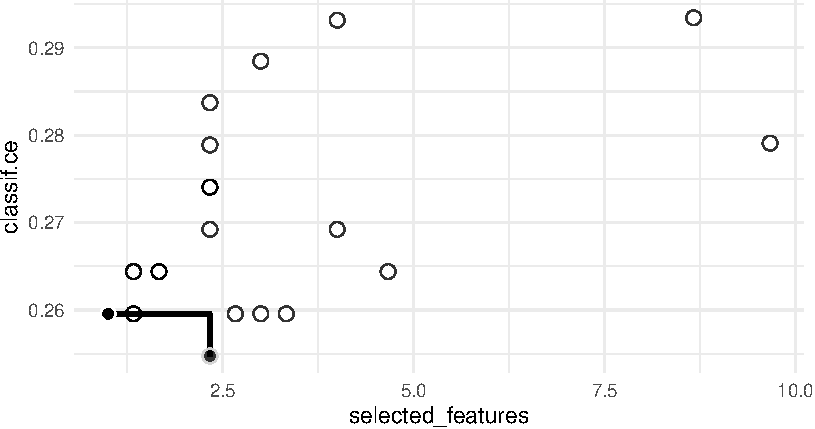
\includegraphics[width=1\textwidth,height=\textheight]{chapters/chapter5/advanced_tuning_methods_and_black_box_optimization_files/figure-pdf/fig-pareto-1.pdf}

}

\caption{\label{fig-pareto}Pareto front of selected features and
classification error. White dots represent tested configurations, each
black dot individually represents a Pareto-optimal configuration and all
black dots together represent the approximated Pareto front.}

\end{figure}

Determining which configuration to deploy from the Pareto front is up to
you. By definition, there is no optimal configuration so this may depend
on your use case, for example, if you would prefer lower complexity at
the cost of higher error then you might prefer a configuration where
\texttt{selected\_features\ =\ 1}.

You can select one configuration and pass it to a learner for training
using \texttt{\$result\_learner\_param\_vals}, so if we want to select
the second configuration we would run:

\begin{Shaded}
\begin{Highlighting}[]
\NormalTok{learner }\OtherTok{=} \FunctionTok{lrn}\NormalTok{(}\StringTok{"classif.rpart"}\NormalTok{)}
\NormalTok{learner}\SpecialCharTok{$}\NormalTok{param\_set}\SpecialCharTok{$}\NormalTok{values }\OtherTok{=}\NormalTok{ instance}\SpecialCharTok{$}\NormalTok{result\_learner\_param\_vals[[}\DecValTok{2}\NormalTok{]]}
\end{Highlighting}
\end{Shaded}

As multi-objective tuning requires manual intervention to select a
configuration, it is currently not possible to use
\href{https://mlr3tuning.mlr-org.com/reference/auto_tuner.html}{\texttt{auto\_tuner()}}.

\hypertarget{sec-hyperband}{%
\section{Multi-Fidelity Tuning via Hyperband}\label{sec-hyperband}}

Increasingly large datasets and search spaces and increasingly complex
models make hyperparameter optimization a time-consuming and
computationally expensive task. To tackle this, some HPO methods make
use of evaluating a configuration at multiple fidelity
levels\index{fidelity}. Multi-fidelity
HPO\index{fidelity!multi-fidelity}{\marginnote{\begin{footnotesize}Multi-fidelity
HPO\end{footnotesize}}} is motivated by the idea that the performance of
a lower-fidelity model is indicative of the full-fidelity model, which
can be used to make HPO more efficient (as we will soon see with
Hyperband).

To unpack what these terms mean and to motivate multi-fidelity tuning,
say that we think a gradient boosting algorithm with up to 1000 rounds
will be a very good fit to our training data. However, we are concerned
this model will take too long to tune and train. Therefore, we want to
gauge the performance of this model using a similar model that is
quicker to train by setting a smaller number of rounds. In this example,
the hyperparameter controlling the number of rounds is a \emph{fidelity
parameter}, as it controls the tradeoff between model performance and
speed. The different configurations of this parameter are known as
\emph{fidelity levels}. We refer to the model with 1000 rounds as the
model at \emph{full-fidelity} and we want to approximate this model's
performance using models at different fidelity levels. Lower fidelity
levels result in low-fidelity models that are quicker to train but may
poorly predict the full-fidelity model's performance. On the other hand,
higher fidelity levels result in high-fidelity models that are slower to
train but may better indicate the full-fidelity model's performance.

Other common models that have natural fidelity parameters include neural
networks\index{neural network} (number of epochs) and random
forests\index{random forest} (number of trees). The proportion of data
to subsample before running any algorithm can also be viewed as a
model-agnostic fidelity parameter, we will return to this in
Section~\ref{sec-hyperband-example-svm}.

\hypertarget{hyperband-and-successive-halving}{%
\subsection{Hyperband and Successive
Halving}\label{hyperband-and-successive-halving}}

A popular multi-fidelity HPO algorithm is \emph{Hyperband} (Li et al.
2018). After having evaluated randomly sampled configurations on low
fidelities, Hyperband\index{hyperband} iteratively allocates more
resources to promising configurations and terminates low-performing ones
early. Hyperband builds upon the Successive Halving algorithm by
Jamieson and Talwalkar (2016). Successive Halving is initialized with a
number of starting configurations \(m_0\), the proportion of
configurations discarded in each stage \(\eta\), and the minimum,
\(r{_{0}}\), and maximum, \(r{_{max}}\), budget (fidelity) of a single
evaluation. The algorithm starts by sampling \(m_0\) random
configurations and allocating the minimum budget \(r{_{0}}\) to them.
The configurations are evaluated and \(\frac{\eta - 1}{\eta}\) of the
worst-performing configurations are discarded. The remaining
configurations are promoted to the next stage, or `bracket', and
evaluated on a larger budget. This continues until one or more
configurations are evaluated on the maximum budget \(r{_{max}}\) and the
best-performing configuration is selected. The total number of stages is
calculated so that each stage consumes approximately the same overall
budget. A big disadvantage of this method is that it is unclear if it is
better to start with many configurations (large \(m_0\)) and a small
budget or fewer configurations (small \(m_0\)) but a larger budget.

Hyperband solves this problem by running Successive Halving with
different numbers of starting configurations, each at different budget
levels \(r_{0}\). The algorithm is initialized with the same \(\eta\)
and \(r_{max}\) parameters (but not \(m_0\)). Each bracket starts with a
different budget, \(r_0\), where smaller values mean that more
configurations can be evaluated and so the most exploratory bracket
(i.e., the one with the most number of stages) is allocated the global
minimum budget \(r_{min}\). In each bracket, the starting budget
increases by a factor of \(\eta\) until the last bracket essentially
performs a random search with the full budget \(r_{max}\). The total
number of brackets, \(s_{max} + 1\), is calculated as
\(s_{max} = {\log_\eta \frac{r_{max}}{r_{min}}}\). The number of
starting configurations \(m_0\) of each bracket are calculated so that
each bracket uses approximately the same amount of budget. The optimal
hyperparameter configuration in each bracket is the configuration with
the best performance in the final stage. The optimal hyperparameter
configuration at the end of tuning is the configuration with the best
performance across all brackets.

An example Hyperband schedule is given in Table~\ref{tbl-hyperband}
where \(s = 3\) is the most exploratory bracket and \(s = 0\)
essentially performs a random search using the full budget.
Table~\ref{tbl-hyperband-eg} demonstrates how this schedule may look if
we were to tune 20 different hyperparameter configurations; note that
each entry in the table is a unique ID referring to a possible
configuration of multiple hyperparameters to tune.

\hypertarget{tbl-hyperband}{}
\begin{longtable}[]{@{}
  >{\raggedright\arraybackslash}p{(\columnwidth - 16\tabcolsep) * \real{0.0645}}
  >{\raggedright\arraybackslash}p{(\columnwidth - 16\tabcolsep) * \real{0.1075}}
  >{\raggedright\arraybackslash}p{(\columnwidth - 16\tabcolsep) * \real{0.1075}}
  >{\raggedright\arraybackslash}p{(\columnwidth - 16\tabcolsep) * \real{0.1075}}
  >{\raggedright\arraybackslash}p{(\columnwidth - 16\tabcolsep) * \real{0.1075}}
  >{\raggedright\arraybackslash}p{(\columnwidth - 16\tabcolsep) * \real{0.1075}}
  >{\raggedright\arraybackslash}p{(\columnwidth - 16\tabcolsep) * \real{0.1075}}
  >{\raggedright\arraybackslash}p{(\columnwidth - 16\tabcolsep) * \real{0.1075}}
  >{\raggedright\arraybackslash}p{(\columnwidth - 16\tabcolsep) * \real{0.1075}}@{}}
\caption{\label{tbl-hyperband}Hyperband schedule with the number of
configurations, \(m_{i}\), and resources, \(r_{i}\), for each bracket,
\(s\), and stage, \(i\), when \(\eta = 2\), \(r{_{min}} = 1\) and
\(r{_{max}} = 8\).}\tabularnewline
\toprule\noalign{}
\begin{minipage}[b]{\linewidth}\raggedright
\end{minipage} &
\multicolumn{2}{>{\raggedright\arraybackslash}p{(\columnwidth - 16\tabcolsep) * \real{0.2151} + 2\tabcolsep}}{%
\begin{minipage}[b]{\linewidth}\raggedright
\(s = 3\)
\end{minipage}} &
\multicolumn{2}{>{\raggedright\arraybackslash}p{(\columnwidth - 16\tabcolsep) * \real{0.2151} + 2\tabcolsep}}{%
\begin{minipage}[b]{\linewidth}\raggedright
\(s = 2\)
\end{minipage}} &
\multicolumn{2}{>{\raggedright\arraybackslash}p{(\columnwidth - 16\tabcolsep) * \real{0.2151} + 2\tabcolsep}}{%
\begin{minipage}[b]{\linewidth}\raggedright
\(s = 1\)
\end{minipage}} &
\multicolumn{2}{>{\raggedright\arraybackslash}p{(\columnwidth - 16\tabcolsep) * \real{0.2151} + 2\tabcolsep}@{}}{%
\begin{minipage}[b]{\linewidth}\raggedright
\(s = 0\)
\end{minipage}} \\
\begin{minipage}[b]{\linewidth}\raggedright
\(i\)
\end{minipage} & \begin{minipage}[b]{\linewidth}\raggedright
\(m_{i}\)
\end{minipage} & \begin{minipage}[b]{\linewidth}\raggedright
\(r_{i}\)
\end{minipage} & \begin{minipage}[b]{\linewidth}\raggedright
\(m_{i}\)
\end{minipage} & \begin{minipage}[b]{\linewidth}\raggedright
\(r_{i}\)
\end{minipage} & \begin{minipage}[b]{\linewidth}\raggedright
\(m_{i}\)
\end{minipage} & \begin{minipage}[b]{\linewidth}\raggedright
\(r_{i}\)
\end{minipage} & \begin{minipage}[b]{\linewidth}\raggedright
\(m_{i}\)
\end{minipage} & \begin{minipage}[b]{\linewidth}\raggedright
\(r_{i}\)
\end{minipage} \\
\midrule\noalign{}
\endfirsthead
\toprule\noalign{}
\begin{minipage}[b]{\linewidth}\raggedright
\end{minipage} &
\multicolumn{2}{>{\raggedright\arraybackslash}p{(\columnwidth - 16\tabcolsep) * \real{0.2151} + 2\tabcolsep}}{%
\begin{minipage}[b]{\linewidth}\raggedright
\(s = 3\)
\end{minipage}} &
\multicolumn{2}{>{\raggedright\arraybackslash}p{(\columnwidth - 16\tabcolsep) * \real{0.2151} + 2\tabcolsep}}{%
\begin{minipage}[b]{\linewidth}\raggedright
\(s = 2\)
\end{minipage}} &
\multicolumn{2}{>{\raggedright\arraybackslash}p{(\columnwidth - 16\tabcolsep) * \real{0.2151} + 2\tabcolsep}}{%
\begin{minipage}[b]{\linewidth}\raggedright
\(s = 1\)
\end{minipage}} &
\multicolumn{2}{>{\raggedright\arraybackslash}p{(\columnwidth - 16\tabcolsep) * \real{0.2151} + 2\tabcolsep}@{}}{%
\begin{minipage}[b]{\linewidth}\raggedright
\(s = 0\)
\end{minipage}} \\
\begin{minipage}[b]{\linewidth}\raggedright
\(i\)
\end{minipage} & \begin{minipage}[b]{\linewidth}\raggedright
\(m_{i}\)
\end{minipage} & \begin{minipage}[b]{\linewidth}\raggedright
\(r_{i}\)
\end{minipage} & \begin{minipage}[b]{\linewidth}\raggedright
\(m_{i}\)
\end{minipage} & \begin{minipage}[b]{\linewidth}\raggedright
\(r_{i}\)
\end{minipage} & \begin{minipage}[b]{\linewidth}\raggedright
\(m_{i}\)
\end{minipage} & \begin{minipage}[b]{\linewidth}\raggedright
\(r_{i}\)
\end{minipage} & \begin{minipage}[b]{\linewidth}\raggedright
\(m_{i}\)
\end{minipage} & \begin{minipage}[b]{\linewidth}\raggedright
\(r_{i}\)
\end{minipage} \\
\midrule\noalign{}
\endhead
\bottomrule\noalign{}
\endlastfoot
0 & 8 & 1 & 6 & 2 & 4 & 4 & 4 & 8 \\
1 & 4 & 2 & 3 & 4 & 2 & 8 & & \\
2 & 2 & 4 & 1 & 8 & & & & \\
3 & 1 & 8 & & & & & & \\
\end{longtable}

\hypertarget{tbl-hyperband-eg}{}
\begin{longtable}[]{@{}
  >{\raggedright\arraybackslash}p{(\columnwidth - 8\tabcolsep) * \real{0.0588}}
  >{\raggedright\arraybackslash}p{(\columnwidth - 8\tabcolsep) * \real{0.2353}}
  >{\raggedright\arraybackslash}p{(\columnwidth - 8\tabcolsep) * \real{0.2353}}
  >{\raggedright\arraybackslash}p{(\columnwidth - 8\tabcolsep) * \real{0.2353}}
  >{\raggedright\arraybackslash}p{(\columnwidth - 8\tabcolsep) * \real{0.2353}}@{}}
\caption{\label{tbl-hyperband-eg}Hyperparameter configurations in each
stage and bracket from the schedule in Table~\ref{tbl-hyperband}.
Entries are unique identifiers for tested hyperparameter configurations
(HPCs). \(HPC^*_s\) is the optimal hyperparameter configuration in
bracket \(s\) and \(HPC^*\) is the optimal hyperparameter configuration
across all brackets.}\tabularnewline
\toprule\noalign{}
\begin{minipage}[b]{\linewidth}\raggedright
\end{minipage} & \begin{minipage}[b]{\linewidth}\raggedright
\(s = 3\)
\end{minipage} & \begin{minipage}[b]{\linewidth}\raggedright
\(s = 2\)
\end{minipage} & \begin{minipage}[b]{\linewidth}\raggedright
\(s = 1\)
\end{minipage} & \begin{minipage}[b]{\linewidth}\raggedright
\(s = 0\)
\end{minipage} \\
\midrule\noalign{}
\endfirsthead
\toprule\noalign{}
\begin{minipage}[b]{\linewidth}\raggedright
\end{minipage} & \begin{minipage}[b]{\linewidth}\raggedright
\(s = 3\)
\end{minipage} & \begin{minipage}[b]{\linewidth}\raggedright
\(s = 2\)
\end{minipage} & \begin{minipage}[b]{\linewidth}\raggedright
\(s = 1\)
\end{minipage} & \begin{minipage}[b]{\linewidth}\raggedright
\(s = 0\)
\end{minipage} \\
\midrule\noalign{}
\endhead
\bottomrule\noalign{}
\endlastfoot
\(i = 0\) & \(\{1, 2, 3, 4, 5, 6, 7, 8\}\) &
\(\{9, 10, 11, 12, 13, 14\}\) & \(\{15, 16, 17, 18\}\) &
\(\{19, 20, 21, 22\}\) \\
\(i = 1\) & \(\{1, 2, 7, 8\}\) & \(\{9, 14, 15\}\) & \(\{20, 21\}\) & \\
\(i = 2\) & \(\{1, 8\}\) & \(\{15\}\) & & \\
\(i = 3\) & \(\{1\}\) & & & \\
\(HPC^*_s\) & \(\{1\}\) & \(\{15\}\) & \(\{21\}\) & \(\{22\}\) \\
\(HPC^*\) & \(\{15\}\) & & & \\
\end{longtable}

\hypertarget{mlr3hyperband}{%
\subsection{mlr3hyperband}\label{mlr3hyperband}}

The Successive Halving and Hyperband algorithms are implemented in
\href{https://mlr3hyperband.mlr-org.com}{\texttt{mlr3hyperband}}\index{\texttt{mlr3hyperband}}
as \texttt{tnr("successive\_halving")} and \texttt{tnr("hyperband")}
respectively; in this section, we will only showcase the Hyperband
method.

By example, we will optimize \texttt{lrn("classif.xgboost")} on
\texttt{tsk("sonar")} and use the number of boosting iterations
(\texttt{nrounds}) as the fidelity parameter, this is a suitable choice
as increasing iterations increases model training time but generally
also improves performance. Hyperband will allocate increasingly more
boosting iterations to well-performing hyperparameter configurations.

We will load the learner and define the search space. We specify a range
from 16 (\(r_{min}\)) to 128 (\(r_{max}\)) boosting iterations and tag
the parameter with \texttt{"budget"} to identify it as a fidelity
parameter. For the other hyperparameters, we take the search space for
XGBoost from Bischl et al. (2023), which usually works well for a wide
range of datasets.

\begin{Shaded}
\begin{Highlighting}[]
\FunctionTok{library}\NormalTok{(mlr3hyperband)}

\NormalTok{learner }\OtherTok{=} \FunctionTok{lrn}\NormalTok{(}\StringTok{"classif.xgboost"}\NormalTok{)}
\NormalTok{learner}\SpecialCharTok{$}\NormalTok{param\_set}\SpecialCharTok{$}\FunctionTok{set\_values}\NormalTok{(}
  \AttributeTok{nrounds           =} \FunctionTok{to\_tune}\NormalTok{(}\FunctionTok{p\_int}\NormalTok{(}\DecValTok{16}\NormalTok{, }\DecValTok{128}\NormalTok{, }\AttributeTok{tags =} \StringTok{"budget"}\NormalTok{)),}
  \AttributeTok{eta               =} \FunctionTok{to\_tune}\NormalTok{(}\FloatTok{1e{-}4}\NormalTok{, }\DecValTok{1}\NormalTok{, }\AttributeTok{logscale =} \ConstantTok{TRUE}\NormalTok{),}
  \AttributeTok{max\_depth         =} \FunctionTok{to\_tune}\NormalTok{(}\DecValTok{1}\NormalTok{, }\DecValTok{20}\NormalTok{),}
  \AttributeTok{colsample\_bytree  =} \FunctionTok{to\_tune}\NormalTok{(}\FloatTok{1e{-}1}\NormalTok{, }\DecValTok{1}\NormalTok{),}
  \AttributeTok{colsample\_bylevel =} \FunctionTok{to\_tune}\NormalTok{(}\FloatTok{1e{-}1}\NormalTok{, }\DecValTok{1}\NormalTok{),}
  \AttributeTok{lambda            =} \FunctionTok{to\_tune}\NormalTok{(}\FloatTok{1e{-}3}\NormalTok{, }\FloatTok{1e3}\NormalTok{, }\AttributeTok{logscale =} \ConstantTok{TRUE}\NormalTok{),}
  \AttributeTok{alpha             =} \FunctionTok{to\_tune}\NormalTok{(}\FloatTok{1e{-}3}\NormalTok{, }\FloatTok{1e3}\NormalTok{, }\AttributeTok{logscale =} \ConstantTok{TRUE}\NormalTok{),}
  \AttributeTok{subsample         =} \FunctionTok{to\_tune}\NormalTok{(}\FloatTok{1e{-}1}\NormalTok{, }\DecValTok{1}\NormalTok{)}
\NormalTok{)}
\end{Highlighting}
\end{Shaded}

We now construct the tuning instance and a hyperband tuner with
\texttt{eta\ =\ 2}. We use \texttt{trm("none")} and set the
\texttt{repetitions} control parameter to \texttt{1} so that Hyperband
can terminate itself after all brackets have been evaluated a single
time. Note that setting \texttt{repetition\ =\ Inf} can be useful if you
want a terminator to stop the optimization, for example, based on
runtime. The
\href{https://mlr3hyperband.mlr-org.com/reference/hyperband_schedule.html}{\texttt{hyperband\_schedule()}}
function can be used to display the schedule across the given fidelity
levels and budget increase factor.

\begin{Shaded}
\begin{Highlighting}[]
\NormalTok{instance }\OtherTok{=} \FunctionTok{ti}\NormalTok{(}
  \AttributeTok{task =} \FunctionTok{tsk}\NormalTok{(}\StringTok{"sonar"}\NormalTok{),}
  \AttributeTok{learner =}\NormalTok{ learner,}
  \AttributeTok{resampling =} \FunctionTok{rsmp}\NormalTok{(}\StringTok{"holdout"}\NormalTok{),}
  \AttributeTok{measures =} \FunctionTok{msr}\NormalTok{(}\StringTok{"classif.ce"}\NormalTok{),}
  \AttributeTok{terminator =} \FunctionTok{trm}\NormalTok{(}\StringTok{"none"}\NormalTok{)}
\NormalTok{)}

\NormalTok{tuner }\OtherTok{=} \FunctionTok{tnr}\NormalTok{(}\StringTok{"hyperband"}\NormalTok{, }\AttributeTok{eta =} \DecValTok{2}\NormalTok{, }\AttributeTok{repetitions =} \DecValTok{1}\NormalTok{)}

\FunctionTok{hyperband\_schedule}\NormalTok{(}\AttributeTok{r\_min =} \DecValTok{16}\NormalTok{, }\AttributeTok{r\_max =} \DecValTok{128}\NormalTok{, }\AttributeTok{eta =} \DecValTok{2}\NormalTok{)}
\end{Highlighting}
\end{Shaded}

\begin{verbatim}
    bracket stage budget n
 1:       3     0     16 8
 2:       3     1     32 4
 3:       3     2     64 2
 4:       3     3    128 1
 5:       2     0     32 6
 6:       2     1     64 3
 7:       2     2    128 1
 8:       1     0     64 4
 9:       1     1    128 2
10:       0     0    128 4
\end{verbatim}

Finally, we can tune as normal and print the result and archive. Note
that the archive resulting from a Hyperband run contains the additional
columns \texttt{bracket} and \texttt{stage} which break down the results
by the corresponding bracket and stage.

\begin{Shaded}
\begin{Highlighting}[]
\NormalTok{tuner}\SpecialCharTok{$}\FunctionTok{optimize}\NormalTok{(instance)}
\end{Highlighting}
\end{Shaded}

\begin{verbatim}
   nrounds    eta max_depth colsample_bytree colsample_bylevel lambda
1:      64 -2.618         3            0.666            0.4722 -5.816
5 variables not shown: [alpha, subsample, learner_param_vals, x_domain, classif.ce]
\end{verbatim}

\begin{Shaded}
\begin{Highlighting}[]
\NormalTok{instance}\SpecialCharTok{$}\NormalTok{result[, .(classif.ce, nrounds)]}
\end{Highlighting}
\end{Shaded}

\begin{verbatim}
   classif.ce nrounds
1:     0.1304      64
\end{verbatim}

\begin{Shaded}
\begin{Highlighting}[]
\FunctionTok{as.data.table}\NormalTok{(instance}\SpecialCharTok{$}\NormalTok{archive)[,}
\NormalTok{  .(bracket, stage, classif.ce, eta, max\_depth, colsample\_bytree)]}
\end{Highlighting}
\end{Shaded}

\begin{verbatim}
    bracket stage classif.ce    eta max_depth colsample_bytree
 1:       3     0     0.4203 -6.664         8           0.8640
 2:       3     0     0.5942 -3.139         2           0.8902
 3:       3     0     0.2899 -6.968        15           0.8204
 4:       3     0     0.2609 -6.555        12           0.6761
 5:       3     0     0.2174 -2.618         3           0.6660
---                                                           
31:       0     0     0.2609 -8.070         1           0.9717
32:       3     3     0.1594 -2.618         3           0.6660
33:       2     2     0.1739 -6.455         5           0.9380
34:       1     1     0.2029 -4.509        10           0.7219
35:       1     1     0.2464 -5.749         3           0.2345
\end{verbatim}

\hypertarget{sec-bayesian-optimization}{%
\section{Bayesian Optimization}\label{sec-bayesian-optimization}}

In this section, we will take a deep dive into Bayesian
optimization\index{Bayesian optimization} (BO), also known as Model
Based Optimization
(MBO)\index{model based optimization|see{Bayesian optimization}}. The
design of BO is more complex than what we have seen so far in other
tuning methods so to help motivate this we will spend a little more time
in this section on theory and methodology.

In hyperparameter optimization\index{hyperparameter optimization}
(Chapter~\ref{sec-optimization}), learners are passed a hyperparameter
configuration and evaluated on a given task via a resampling technique
to estimate its generalization performance with the goal to find the
optimal hyperparameter configuration. In general, no analytical
description for the mapping from hyperparameter configuration to
performance exists and gradient information is also not available. HPO
is, therefore, a prime example for black box
optimization\index{black box optimization}{\marginnote{\begin{footnotesize}Black
Box Optimization\end{footnotesize}}}, which considers the optimization
of a function whose mathematical structure and analytical description is
unknown or unexploitable. As a result, the only observable information
is the output value (i.e., generalization performance) of the function
given an input value (i.e., hyperparameter configuration). In fact, as
evaluating the performance of a learner can take a substantial amount of
time, HPO is quite an expensive black box optimization problem. Black
box optimization problems occur in the real-world, for example they are
encountered quite often in engineering such as in modeling experiments
like crash tests or chemical reactions.

Many optimization algorithm classes exist that can be used for black box
optimization, which differ in how they tackle this problem; for example
we saw in Chapter~\ref{sec-optimization} methods including grid/random
search and briefly discussed evolutionary strategies. Bayesian
optimization refers to a class of sample-efficient iterative global
black box optimization algorithms that rely on a `surrogate model'
trained on observed data to model the black box function. This surrogate
model is typically a non-linear regression model that tries to capture
the unknown function using limited observed data. During each iteration,
BO algorithms employ an `acquisition function' to determine the next
candidate point for evaluation. This function measures the expected
`utility' of each point within the search space based on the prediction
of the surrogate model. The algorithm then selects the candidate point
with the best acquisition function value and evaluates the black box
function at that point to then update the surrogate model. This
iterative process continues until a termination criterion is met, such
as reaching a pre-specified maximum number of evaluations or achieving a
desired level of performance. BO is a powerful method that often results
in good optimization performance, especially if the cost of the black
box evaluation becomes expensive and the optimization budget is tight.

In the rest of this section, we will first provide an introduction to
black box optimization with the
\href{https://bbotk.mlr-org.com}{\texttt{bbotk}}\index{\texttt{bbotk}}
package and then introduce the building blocks of BO algorithms and
examine their interplay and interaction during the optimization process
before we assemble these building blocks in a ready to use black box
optimizer with
\href{https://mlr3mbo.mlr-org.com}{\texttt{mlr3mbo}}\index{\texttt{mlr3mbo}}.
Readers who are primarily interested in how to utilize BO for HPO
without delving deep into the underlying building blocks may want to
skip to Section~\ref{sec-bayesian-tuning}. Detailed introductions to
black box optimization and BO are given in Bischl et al. (2023), Feurer
and Hutter (2019) and Garnett (2022).

As a running example throughout this section, we will optimize the
sinusoidal function
\(f: [0, 1] \rightarrow \mathbb{R}, x \mapsto 2x + \sin(14x)\)
(Figure~\ref{fig-bayesian-optimization-sinusoidal}), which is
characterized by two local minima and one global minimum.

\hypertarget{sec-black-box-optimization}{%
\subsection{Black Box Optimization}\label{sec-black-box-optimization}}

The
\href{https://bbotk.mlr-org.com}{\texttt{bbotk}}\index{\texttt{bbotk}}
(black box optimization toolkit) package is the workhorse package for
general black box optimization within the \texttt{mlr3} ecosystem. At
the heart of the package are the R6 classes:

\begin{itemize}
\tightlist
\item
  \href{https://bbotk.mlr-org.com/reference/OptimInstanceSingleCrit.html}{\texttt{OptimInstanceSingleCrit}}
  and
  \href{https://bbotk.mlr-org.com/reference/OptimInstanceMultiCrit.html}{\texttt{OptimInstanceMultiCrit}},
  which are used to construct an optimization
  instance\index{optimization instance}{\marginnote{\begin{footnotesize}Optimization
  Instance\end{footnotesize}}} that describes the optimization problem
  and stores the results
\item
  \href{https://bbotk.mlr-org.com/reference/Optimizer.html}{\texttt{Optimizer}}
  which is used to construct and configure optimization algorithms.
\end{itemize}

These classes might look familiar after reading
Chapter~\ref{sec-optimization}, and in fact
\href{https://mlr3tuning.mlr-org.com/reference/TuningInstanceSingleCrit.html}{\texttt{TuningInstanceSingleCrit}}
and
\href{https://mlr3tuning.mlr-org.com/reference/TuningInstanceMultiCrit.html}{\texttt{TuningInstanceMultiCrit}}
inherit from \texttt{OptimInstanceSingle/MultiCrit} and
\href{https://mlr3tuning.mlr-org.com/reference/Tuner.html}{\texttt{Tuner}}
is closely based on \texttt{Optimizer}.

\texttt{OptimInstanceSingleCrit} relies on an
\href{https://bbotk.mlr-org.com/reference/Objective.html}{\texttt{Objective}}\index{\texttt{Objective}}{\marginnote{\begin{footnotesize}\texttt{Objective}\end{footnotesize}}}
function that wraps the actual mapping from a domain (all possible
function inputs) to a codomain (all possible function outputs).

Objective functions can be created using different classes, all of which
inherit from
\href{https://bbotk.mlr-org.com/reference/Objective.html}{\texttt{Objective}}.
These classes provide different ways to define and evaluate objective
functions and picking the right one will reduce type conversion
overhead:

\begin{itemize}
\tightlist
\item
  \href{https://bbotk.mlr-org.com/reference/ObjectiveRFun.html}{\texttt{ObjectiveRFun}}
  wraps a function that takes a list describing a \emph{single
  configuration} as input where elements can be of any type. It is
  suitable when the underlying function evaluation mechanism is given by
  evaluating a single configuration at a time.
\item
  \href{https://bbotk.mlr-org.com/reference/ObjectiveRFunMany.html}{\texttt{ObjectiveRFunMany}}
  wraps a function that takes a list of \emph{multiple configurations}
  as input where elements can be of any type and even mixed types. It is
  useful when the function evaluation of multiple configurations can be
  parallelized.
\item
  \href{https://bbotk.mlr-org.com/reference/ObjectiveRFunDt.html}{\texttt{ObjectiveRFunDt}}
  wraps a function that operates on a \texttt{data.table}. It allows for
  efficient vectorized or batched evaluations directly on the
  \texttt{data.table} object, avoiding unnecessary data type
  conversions.
\end{itemize}

To start translating our problem to code we will use the
\href{https://bbotk.mlr-org.com/reference/ObjectiveRFun.html}{\texttt{ObjectiveRFun}}
class to take a single configuration as input. The \texttt{Objective}
requires specification of the function to optimize its domain and
codomain. By tagging the codomain with \texttt{"minimize"} or
\texttt{"maximize"} we specify the optimization direction. Note how
below our optimization function takes a \texttt{list} as an input with
one element called \texttt{x}.

\begin{Shaded}
\begin{Highlighting}[]
\FunctionTok{library}\NormalTok{(bbotk)}
\NormalTok{sinus\_1D }\OtherTok{=} \ControlFlowTok{function}\NormalTok{(xs) }\DecValTok{2} \SpecialCharTok{*}\NormalTok{ xs}\SpecialCharTok{$}\NormalTok{x }\SpecialCharTok{*} \FunctionTok{sin}\NormalTok{(}\DecValTok{14} \SpecialCharTok{*}\NormalTok{ xs}\SpecialCharTok{$}\NormalTok{x)}

\NormalTok{domain }\OtherTok{=} \FunctionTok{ps}\NormalTok{(}\AttributeTok{x =} \FunctionTok{p\_dbl}\NormalTok{(}\AttributeTok{lower =} \DecValTok{0}\NormalTok{, }\AttributeTok{upper =} \DecValTok{1}\NormalTok{))}
\NormalTok{codomain }\OtherTok{=} \FunctionTok{ps}\NormalTok{(}\AttributeTok{y =} \FunctionTok{p\_dbl}\NormalTok{(}\AttributeTok{tags =} \StringTok{"minimize"}\NormalTok{))}
\NormalTok{objective }\OtherTok{=}\NormalTok{ ObjectiveRFun}\SpecialCharTok{$}\FunctionTok{new}\NormalTok{(sinus\_1D,}
  \AttributeTok{domain =}\NormalTok{ domain, }\AttributeTok{codomain =}\NormalTok{ codomain)}
\end{Highlighting}
\end{Shaded}

We can visualize our objective by generating a grid of points on which
we evaluate the function
(Figure~\ref{fig-bayesian-optimization-sinusoidal}), this will help us
identify its local minima and global minimum.

\begin{Shaded}
\begin{Highlighting}[]
\FunctionTok{library}\NormalTok{(ggplot2)}

\NormalTok{xydt }\OtherTok{=} \FunctionTok{generate\_design\_grid}\NormalTok{(domain, }\AttributeTok{resolution =} \DecValTok{1001}\NormalTok{)}\SpecialCharTok{$}\NormalTok{data}
\NormalTok{xydt[, y }\SpecialCharTok{:}\ErrorTok{=}\NormalTok{ objective}\SpecialCharTok{$}\FunctionTok{eval\_dt}\NormalTok{(xydt)}\SpecialCharTok{$}\NormalTok{y]}
\NormalTok{optima }\OtherTok{=} \FunctionTok{data.table}\NormalTok{(}\AttributeTok{x =} \FunctionTok{c}\NormalTok{(}\DecValTok{0}\NormalTok{, }\FloatTok{0.3509406}\NormalTok{, }\FloatTok{0.7918238}\NormalTok{))}
\NormalTok{optima[, y }\SpecialCharTok{:}\ErrorTok{=}\NormalTok{ objective}\SpecialCharTok{$}\FunctionTok{eval\_dt}\NormalTok{(optima)}\SpecialCharTok{$}\NormalTok{y]}
\NormalTok{optima[, type }\SpecialCharTok{:}\ErrorTok{=} \FunctionTok{c}\NormalTok{(}\StringTok{"local"}\NormalTok{, }\StringTok{"local"}\NormalTok{, }\StringTok{"global"}\NormalTok{)]}

\FunctionTok{ggplot}\NormalTok{(}\FunctionTok{aes}\NormalTok{(}\AttributeTok{x =}\NormalTok{ x, }\AttributeTok{y =}\NormalTok{ y), }\AttributeTok{data =}\NormalTok{ xydt) }\SpecialCharTok{+}
  \FunctionTok{geom\_line}\NormalTok{() }\SpecialCharTok{+}
  \FunctionTok{geom\_point}\NormalTok{(}\FunctionTok{aes}\NormalTok{(}\AttributeTok{pch =}\NormalTok{ type), }\AttributeTok{color =} \StringTok{"black"}\NormalTok{, }\AttributeTok{size =} \DecValTok{4}\NormalTok{, }\AttributeTok{data =}\NormalTok{ optima) }\SpecialCharTok{+}
  \FunctionTok{theme\_minimal}\NormalTok{() }\SpecialCharTok{+}
  \FunctionTok{theme}\NormalTok{(}\AttributeTok{legend.position =} \StringTok{"none"}\NormalTok{)}
\end{Highlighting}
\end{Shaded}

\begin{figure}[H]

{\centering 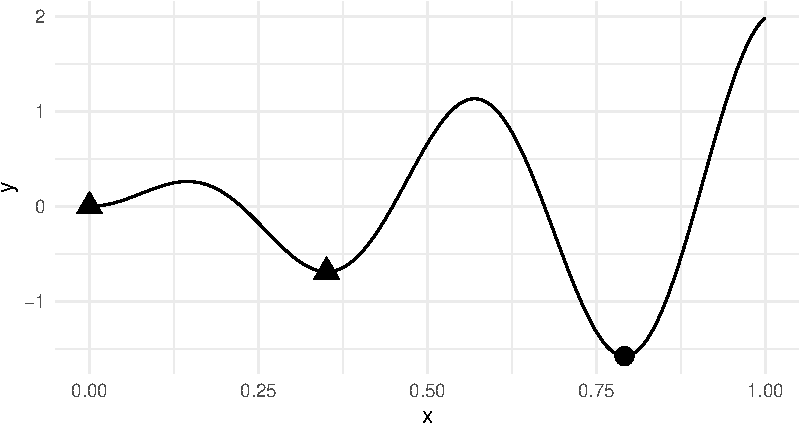
\includegraphics[width=1\textwidth,height=\textheight]{chapters/chapter5/advanced_tuning_methods_and_black_box_optimization_files/figure-pdf/fig-bayesian-optimization-sinusoidal-1.pdf}

}

\caption{\label{fig-bayesian-optimization-sinusoidal}Visualization of
the sinusoidal function. Local minima in triangles and global minimum in
the circle.}

\end{figure}

The global minimizer, 0.792, corresponds to the point of the domain with
the lowest function value:

\begin{Shaded}
\begin{Highlighting}[]
\NormalTok{xydt[y }\SpecialCharTok{==} \FunctionTok{min}\NormalTok{(y), ]}
\end{Highlighting}
\end{Shaded}

\begin{verbatim}
       x      y
1: 0.792 -1.577
\end{verbatim}

With the objective function defined, we can proceed to optimize it using
\texttt{OptimInstanceSingleCrit}. This class allows us to wrap the
objective function and explicitly specify a search space. The search
space defines the set of input values we want to optimize over, and it
is typically a subset or transformation of the domain, though by default
the entire domain is taken as the search space. In black box
optimization, it is common for the domain, and hence also the search
space, to have finite box constraints. Similarly to HPO, transformations
can sometimes be used to more efficiently search the space
(Section~\ref{sec-logarithmic-transformations}).

In the following, we use a simple random search to optimize the
sinusoidal function over the whole domain and inspect the result from
the \texttt{instance} in the usual way (Section~\ref{sec-tuner}).
Analogously to tuners, \texttt{Optimizer}s in \texttt{bbotk} are stored
in the
\href{https://bbotk.mlr-org.com/reference/mlr_optimizers.html}{\texttt{mlr\_optimizers}}
dictionary and can be constructed with
\href{https://bbotk.mlr-org.com/reference/opt.html}{\texttt{opt()}}\index{\texttt{opt()}}{\marginnote{\begin{footnotesize}\texttt{opt()}\end{footnotesize}}}.

\begin{Shaded}
\begin{Highlighting}[]
\NormalTok{instance }\OtherTok{=}\NormalTok{ OptimInstanceSingleCrit}\SpecialCharTok{$}\FunctionTok{new}\NormalTok{(objective,}
  \AttributeTok{search\_space =}\NormalTok{ domain,}
  \AttributeTok{terminator =} \FunctionTok{trm}\NormalTok{(}\StringTok{"evals"}\NormalTok{, }\AttributeTok{n\_evals =} \DecValTok{20}\NormalTok{))}
\NormalTok{optimizer }\OtherTok{=} \FunctionTok{opt}\NormalTok{(}\StringTok{"random\_search"}\NormalTok{, }\AttributeTok{batch\_size =} \DecValTok{20}\NormalTok{)}
\NormalTok{optimizer}\SpecialCharTok{$}\FunctionTok{optimize}\NormalTok{(instance)}
\end{Highlighting}
\end{Shaded}

Similarly to how we can use
\href{https://mlr3tuning.mlr-org.com/reference/tune.html}{\texttt{tune()}}
to construct a tuning instance, here we can use
\href{https://bbotk.mlr-org.com/reference/bb_optimize.html}{\texttt{bb\_optimize()}},
which returns a list with elements \texttt{"par"} (best found
parameters), \texttt{"val"} (optimal outcome), and \texttt{"instance"}
(the optimization instance); the values given as \texttt{"par"} and
\texttt{"val"} are the same as the values found in
\texttt{instance\$result}:

\begin{Shaded}
\begin{Highlighting}[]
\NormalTok{optimal }\OtherTok{=} \FunctionTok{bb\_optimize}\NormalTok{(objective, }\AttributeTok{method =} \StringTok{"random\_search"}\NormalTok{,}
  \AttributeTok{max\_evals =} \DecValTok{20}\NormalTok{)}
\NormalTok{optimal}\SpecialCharTok{$}\NormalTok{instance}\SpecialCharTok{$}\NormalTok{result}
\end{Highlighting}
\end{Shaded}

\begin{verbatim}
        x  x_domain      y
1: 0.7377 <list[1]> -1.158
\end{verbatim}

Now we have introduced the basic black box optimization setup, we can
introduce the building blocks of any Bayesian optimization algorithm.

\hypertarget{sec-bayesian-optimization-blocks}{%
\subsection{Building Blocks of Bayesian
Optimization}\label{sec-bayesian-optimization-blocks}}

Bayesian optimization (BO) is a global optimization algorithm that
usually follows the following process
(Figure~\ref{fig-optimization-loop}):

\begin{enumerate}
\def\labelenumi{\arabic{enumi}.}
\tightlist
\item
  Generate and evaluate an initial design\index{initial design}
\item
  Loop:

  \begin{enumerate}
  \def\labelenumii{\alph{enumii}.}
  \tightlist
  \item
    Fit a surrogate model\index{surrogate model} on the archive of all
    observations made so far to model the unknown black box function.
  \item
    Optimize an acquisition function\index{acquisition function} to
    determine which points of the search space are promising
    candidate(s) that should be evaluated next.
  \item
    Evaluate the next candidate(s) and update the archive of all
    observations made so far.
  \item
    Check if a given termination criterion is met, if not go back to
    (a).
  \end{enumerate}
\end{enumerate}

The acquisition function relies on the mean and standard deviation
prediction of the surrogate model and requires no evaluation of the true
black box function, making it comparably cheap to optimize. A good
acquisition function will balance \emph{exploiting} knowledge about
regions where we observed that performance is good and the surrogate
model has low uncertainty, with \emph{exploring} regions where it has
not yet evaluated points and as a result the uncertainty of the
surrogate model is high.

We refer to these elements as the `building blocks' of BO as it is a
highly modular algorithm; as long as the above structure is in place,
then the surrogate models, acquisition functions, and acquisition
function optimizers are all interchangeable to a certain extent. The
design of \texttt{mlr3mbo} reflects this modularity, with the base class
for
\href{https://mlr3mbo.mlr-org.com/reference/mlr_optimizers_mbo.html}{\texttt{OptimizerMbo}}
holding all the key elements: the BO algorithm loop structure
(\href{https://mlr3mbo.mlr-org.com/reference/loop_function.html}{\texttt{loop\_function}}),
\emph{surrogate} model
(\href{https://mlr3mbo.mlr-org.com/reference/Surrogate.html}{\texttt{Surrogate}}),
\emph{acquisition function}
(\href{https://mlr3mbo.mlr-org.com/reference/AcqFunction.html}{\texttt{AcqFunction}}),
and \emph{acquisition function optimizer}
(\href{https://mlr3mbo.mlr-org.com/reference/AcqOptimizer.html}{\texttt{AcqOptimizer}}).
In this section, we will provide a more detailed explanation of these
building blocks and explore their interplay and interaction during
optimization.

\begin{figure}

{\centering 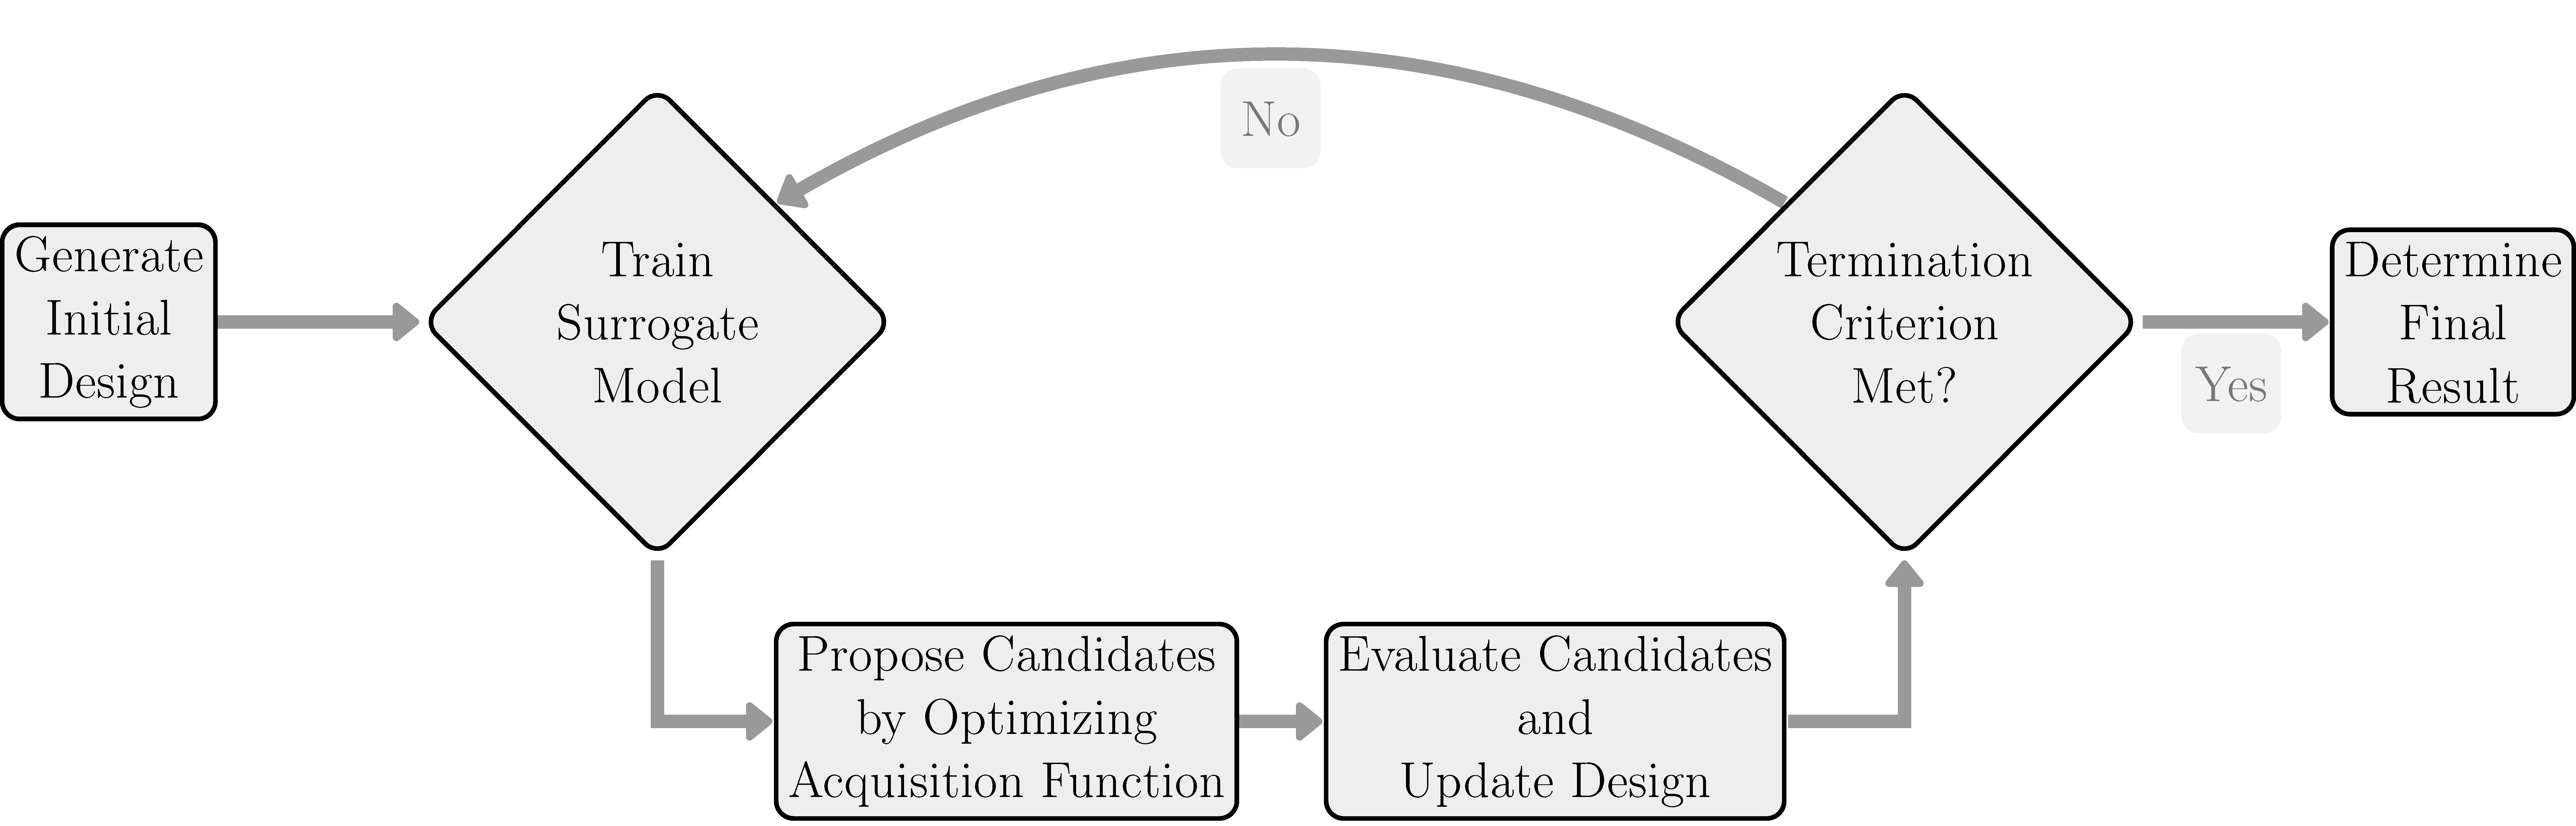
\includegraphics[width=0.8\textwidth,height=\textheight]{chapters/chapter5/Figures/mlr3book_figures-10.png}

}

\caption{\label{fig-optimization-loop}Bayesian optimization loop.}

\end{figure}

\hypertarget{sec-bayesian-optimization-initial}{%
\subsubsection{The Initial
Design}\label{sec-bayesian-optimization-initial}}

Before we can fit a surrogate model to model the unknown black box
function, we need data. The initial set of points that is evaluated
before a surrogate model can be fit is referred to as the initial
design\index{initial design}.

\texttt{mlr3mbo} allows you to either construct the initial design
manually or let a
\href{https://mlr3mbo.mlr-org.com/reference/loop_function.html}{\texttt{loop\_function}}
construct and evaluate this for you. In this section, we will
demonstrate the first method, which requires more user input but
therefore allows more control over the initial design.

A simple method to construct an initial design is to use one of the four
design generators in
\href{https://paradox.mlr-org.com}{\texttt{paradox}}\index{\texttt{paradox}}:

\begin{itemize}
\tightlist
\item
  \href{https://paradox.mlr-org.com/reference/generate_design_random.html}{\texttt{generate\_design\_random()}}:
  Generate points uniformly at random
\item
  \href{https://paradox.mlr-org.com/reference/generate_design_grid.html}{\texttt{generate\_design\_grid()}}:
  Generate points in a uniform-sized grid
\item
  \href{https://paradox.mlr-org.com/reference/generate_design_lhs.html}{\texttt{generate\_design\_lhs()}}:
  Latin hypercube sampling (Stein 1987)
\item
  \href{https://paradox.mlr-org.com/reference/generate_design_sobol.html}{\texttt{generate\_design\_sobol()}}:
  Sobol sequence (Niederreiter 1988)
\end{itemize}

Figure~\ref{fig-bayesian-optimization-designs} illustrates the
difference in generated designs from these four methods assuming an
initial design of size nine and a domain of two numeric variables from
\(0\) to \(1\). We already covered the difference between grid and
random designs in Section~\ref{sec-tuner}. An LHS design divides each
input variable into equally sized intervals (indicated by the horizontal
and vertical dotted lines in
Figure~\ref{fig-bayesian-optimization-designs}) and ensures that each
interval is represented by exactly one sample point, resulting in
uniform marginal distributions. Furthermore, in LHS designs the minimal
distance between two points is usually maximized, resulting in its
space-filling coverage of the space. The Sobol design works similarly to
LHS but can provide better coverage than LHS when the number of
dimensions is large. For this reason, LHS or Sobol designs are usually
recommended for BO, but usually the influence of the initial design will
be smaller compared to other design choices of BO. A random design might
work well-enough, but grid designs are usually discouraged.

\begin{figure}

{\centering 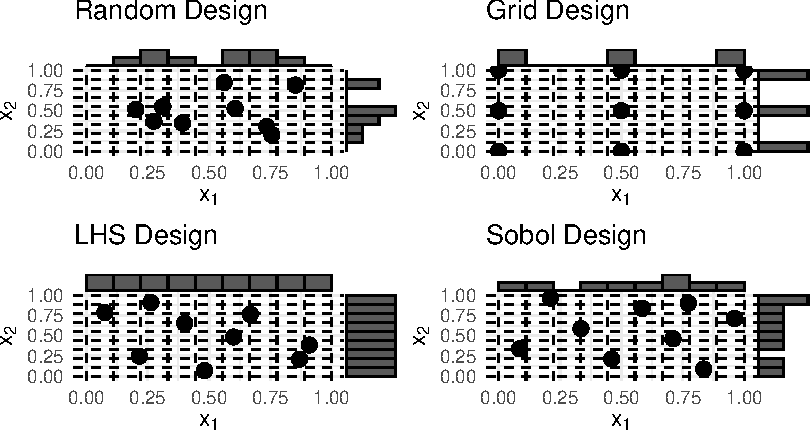
\includegraphics[width=1\textwidth,height=\textheight]{chapters/chapter5/advanced_tuning_methods_and_black_box_optimization_files/figure-pdf/fig-bayesian-optimization-designs-1.pdf}

}

\caption{\label{fig-bayesian-optimization-designs}Comparing different
samplers for constructing an initial design of nine points on a domain
of two numeric variables ranging from \(0\) to \(1\). Dotted horizontal
and vertical lines partition the domain into equally sized bins.
Histograms on the top and right visualize the marginal distributions of
the generated sample.}

\end{figure}

Whichever of these methods you choose, the result is a
\href{https://paradox.mlr-org.com/reference/Design.html}{\texttt{Design}}
object, which is mostly just a wrapper around a \texttt{data.table}:

\begin{Shaded}
\begin{Highlighting}[]
\NormalTok{sample\_domain }\OtherTok{=} \FunctionTok{ps}\NormalTok{(}\AttributeTok{x1 =} \FunctionTok{p\_dbl}\NormalTok{(}\DecValTok{0}\NormalTok{, }\DecValTok{1}\NormalTok{), }\AttributeTok{x2 =} \FunctionTok{p\_dbl}\NormalTok{(}\DecValTok{0}\NormalTok{, }\DecValTok{1}\NormalTok{))}
\FunctionTok{generate\_design\_random}\NormalTok{(sample\_domain, }\AttributeTok{n =} \DecValTok{3}\NormalTok{)}\SpecialCharTok{$}\NormalTok{data}
\end{Highlighting}
\end{Shaded}

\begin{verbatim}
       x1     x2
1: 0.9930 0.3773
2: 0.6782 0.4612
3: 0.4355 0.8019
\end{verbatim}

Therefore you could also specify a completely custom initial design by
defining your own \texttt{data.table}. Either way, when manually
constructing an initial design (as opposed to letting
\texttt{loop\_function} automate this), it needs to be evaluated on the
\href{https://bbotk.mlr-org.com/reference/OptimInstance.html}{\texttt{OptimInstance}}
before optimizing it. Returning to our running example of minimizing the
sinusoidal function, we will evaluate a custom initial design with
\texttt{\$eval\_batch()}:

\begin{Shaded}
\begin{Highlighting}[]
\NormalTok{instance }\OtherTok{=}\NormalTok{ OptimInstanceSingleCrit}\SpecialCharTok{$}\FunctionTok{new}\NormalTok{(objective,}
  \AttributeTok{terminator =} \FunctionTok{trm}\NormalTok{(}\StringTok{"evals"}\NormalTok{, }\AttributeTok{n\_evals =} \DecValTok{20}\NormalTok{))}
\NormalTok{design }\OtherTok{=} \FunctionTok{data.table}\NormalTok{(}\AttributeTok{x =} \FunctionTok{c}\NormalTok{(}\FloatTok{0.1}\NormalTok{, }\FloatTok{0.34}\NormalTok{, }\FloatTok{0.65}\NormalTok{, }\DecValTok{1}\NormalTok{))}
\NormalTok{instance}\SpecialCharTok{$}\FunctionTok{eval\_batch}\NormalTok{(design)}
\NormalTok{instance}\SpecialCharTok{$}\NormalTok{archive}\SpecialCharTok{$}\NormalTok{data}
\end{Highlighting}
\end{Shaded}

\begin{verbatim}
      x       y  x_domain           timestamp batch_nr
1: 0.10  0.1971 <list[1]> 2023-07-04 15:25:40        1
2: 0.34 -0.6792 <list[1]> 2023-07-04 15:25:40        1
3: 0.65  0.4148 <list[1]> 2023-07-04 15:25:40        1
4: 1.00  1.9812 <list[1]> 2023-07-04 15:25:40        1
\end{verbatim}

We can see how each point in our design was evaluated by the sinusoidal
function, giving us data we can now use to start the iterative BO
algorithm by fitting the surrogate model on that data.

\hypertarget{sec-bayesian-optimization-surrogate}{%
\subsubsection{Surrogate
Model}\label{sec-bayesian-optimization-surrogate}}

A surrogate model\index{surrogate model} wraps a regression learner that
models the unknown black box function based on observed data. In
\texttt{mlr3mbo}, the
\href{https://mlr3mbo.mlr-org.com/reference/SurrogateLearner.html}{\texttt{SurrogateLearner}}
is a higher-level R6 class inheriting from the base
\href{https://mlr3mbo.mlr-org.com/reference/Surrogate.html}{\texttt{Surrogate}}
class, designed to construct and manage the surrogate model, including
automatic construction of the \texttt{TaskRegr} that the learner should
be trained on at each iteration of the BO loop.

Any regression learner in \texttt{mlr3} can be used. However, most
acquisition functions depend on both mean and standard deviation
predictions from the surrogate model, the latter of which requires the
\texttt{"se"} \texttt{predict\_type} to be supported. Therefore not all
learners are suitable for all scenarios. Typical choices of regression
learners used as surrogate models include Gaussian
processes\index{Gaussian process} (\texttt{lrn("regr.km")}) for low to
medium dimensional numeric search spaces and random
forests\index{random forest} (e.g., \texttt{lrn("regr.ranger")}) for
higher dimensional mixed (and/or hierarchical) search spaces. A detailed
introduction to Gaussian processes can be found in Williams and
Rasmussen (2006) and an in-depth focus on Gaussian processes in the
context of surrogate models in BO is given in Garnett (2022). In this
example, we use a Gaussian process with Matérn 5/2 kernel, which uses
\texttt{BFGS} as an optimizer to find the optimal kernel parameters and
set \texttt{trace\ =\ FALSE} to prevent too much output during fitting.

\begin{Shaded}
\begin{Highlighting}[]
\NormalTok{lrn\_gp }\OtherTok{=} \FunctionTok{lrn}\NormalTok{(}\StringTok{"regr.km"}\NormalTok{, }\AttributeTok{covtype =} \StringTok{"matern5\_2"}\NormalTok{, }\AttributeTok{optim.method =} \StringTok{"BFGS"}\NormalTok{,}
  \AttributeTok{control =} \FunctionTok{list}\NormalTok{(}\AttributeTok{trace =} \ConstantTok{FALSE}\NormalTok{))}
\end{Highlighting}
\end{Shaded}

A \texttt{SurrogateLearner} can be constructed by passing a
\texttt{LearnerRegr} object to the sugar function
\texttt{srlrn()}\index{\texttt{srlrn()}}{\marginnote{\begin{footnotesize}srlrn()\end{footnotesize}}},
alongside the \texttt{archive} of the instance:

\begin{Shaded}
\begin{Highlighting}[]
\FunctionTok{library}\NormalTok{(mlr3mbo)}
\NormalTok{surrogate }\OtherTok{=} \FunctionTok{srlrn}\NormalTok{(lrn\_gp, }\AttributeTok{archive =}\NormalTok{ instance}\SpecialCharTok{$}\NormalTok{archive)}
\end{Highlighting}
\end{Shaded}

Internally, the regression learner is fit on a \texttt{TaskRegr} where
features are the variables of the domain and the target is the codomain,
the data is from the
\href{https://bbotk.mlr-org.com/reference/Archive.html}{\texttt{Archive}}
of the
\href{https://bbotk.mlr-org.com/reference/OptimInstance.html}{\texttt{OptimInstance}}
that is to be optimized.

In our running example we have already initialized our archive with the
initial design, so we can update our surrogate model, which essentially
fits the Gaussian process, note how we use \texttt{\$learner} to access
the wrapped model:

\begin{Shaded}
\begin{Highlighting}[]
\NormalTok{surrogate}\SpecialCharTok{$}\FunctionTok{update}\NormalTok{()}
\NormalTok{surrogate}\SpecialCharTok{$}\NormalTok{learner}\SpecialCharTok{$}\NormalTok{model}
\end{Highlighting}
\end{Shaded}

\begin{verbatim}

Call:
DiceKriging::km(design = data, response = task$truth(), covtype = "matern5_2", 
    optim.method = "BFGS", control = pv$control)

Trend  coeff.:
               Estimate
 (Intercept)     0.7899

Covar. type  : matern5_2 
Covar. coeff.:
               Estimate
    theta(x)     0.3014

Variance estimate: 1.07
\end{verbatim}

Having introduced the concept of a surrogate model, we can now move on
to the acquisition function, which makes use of the surrogate model
predictions to decide which candidate to evaluate next.

\hypertarget{sec-bayesian-optimization-acquisition}{%
\subsubsection{Acquisition
Function}\label{sec-bayesian-optimization-acquisition}}

Roughly speaking, an acquisition function\index{acquisition function}
relies on the prediction of a surrogate model and quantifies the
expected `utility' of each point of the search space if it were to be
evaluated in the next iteration.

A popular example is the expected improvement (Jones, Schonlau, and
Welch 1998), which tells us how much we can expect a candidate point to
improve over the best function value observed so far (the `incumbent'),
given the performance prediction of the surrogate model:

\[
\alpha_{\mathrm{EI}}(\mathbf{x}) = \mathbb{E} \left[ \max \left( f_{\mathrm{min}} - Y(\mathbf{x}), 0 \right) \right]
\]

Here, \(Y(\mathbf{x)}\) is the surrogate model prediction (a random
variable) for a given point \(\mathbf{x}\) (which when using a Gaussian
process follows a normal distribution) and \(f_{\mathrm{min}}\) is the
best function value observed so far (assuming minimization). Calculating
the expected improvement requires mean and standard deviation
predictions from the model.

In \texttt{mlr3mbo}, acquisition functions (of class
\href{https://mlr3mbo.mlr-org.com/reference/AcqFunction.html}{\texttt{AcqFunction}})
are stored in the
\href{https://mlr3mbo.mlr-org.com/reference/mlr_acqfunctions.html}{\texttt{mlr\_acqfunctions}}
dictionary and can be constructed with
\href{https://mlr3mbo.mlr-org.com/reference/acqf.html}{\texttt{acqf()}}\index{\texttt{acqf()}}{\marginnote{\begin{footnotesize}\texttt{acqf()}\end{footnotesize}}},
passing the key of the method you want to use and our surrogate learner.
In our running example, we will use the expected improvement
(\texttt{acqf("ei")}) to choose the next candidate for evaluation.
Before we can do that, we have to update (\texttt{\$update()}) the
\texttt{AcqFunction}'s view of the incumbent, to ensure it is still
using the best value observed so far.

\begin{Shaded}
\begin{Highlighting}[]
\NormalTok{acq\_function }\OtherTok{=} \FunctionTok{acqf}\NormalTok{(}\StringTok{"ei"}\NormalTok{, }\AttributeTok{surrogate =}\NormalTok{ surrogate)}
\NormalTok{acq\_function}\SpecialCharTok{$}\FunctionTok{update}\NormalTok{()}
\NormalTok{acq\_function}\SpecialCharTok{$}\NormalTok{y\_best}
\end{Highlighting}
\end{Shaded}

\begin{verbatim}
[1] -0.6792
\end{verbatim}

You can use \texttt{\$eval\_dt()} to evaluate the acquisition function
for the domain given as a \texttt{data.table}. In
Figure~\ref{fig-bayesian-optimization-ei} we evaluated the expected
improvement on a uniform grid of points between \(0\) and \(1\) using
the predicted mean and standard deviation from the Gaussian process. We
can see that the expected improvement is high in regions where the mean
prediction (gray dashed lines) of the Gaussian process is low, or where
the uncertainty is high.

\begin{Shaded}
\begin{Highlighting}[]
\NormalTok{xydt }\OtherTok{=} \FunctionTok{generate\_design\_grid}\NormalTok{(domain, }\AttributeTok{resolution =} \DecValTok{1001}\NormalTok{)}\SpecialCharTok{$}\NormalTok{data}
\CommentTok{\# evaluate our sinusoidal function}
\NormalTok{xydt[, y }\SpecialCharTok{:}\ErrorTok{=}\NormalTok{ objective}\SpecialCharTok{$}\FunctionTok{eval\_dt}\NormalTok{(xydt)}\SpecialCharTok{$}\NormalTok{y]}
\CommentTok{\# evaluate expected improvement}
\NormalTok{xydt[, ei }\SpecialCharTok{:}\ErrorTok{=}\NormalTok{  acq\_function}\SpecialCharTok{$}\FunctionTok{eval\_dt}\NormalTok{(xydt[, }\StringTok{"x"}\NormalTok{])]}
\CommentTok{\# make predictions from our data}
\NormalTok{xydt[, }\FunctionTok{c}\NormalTok{(}\StringTok{"mean"}\NormalTok{, }\StringTok{"se"}\NormalTok{) }\SpecialCharTok{:}\ErrorTok{=}\NormalTok{  surrogate}\SpecialCharTok{$}\FunctionTok{predict}\NormalTok{(xydt[, }\StringTok{"x"}\NormalTok{])]}
\NormalTok{xydt[}\DecValTok{1}\SpecialCharTok{:}\DecValTok{3}\NormalTok{]}
\end{Highlighting}
\end{Shaded}

\begin{verbatim}
       x        y        ei   mean     se
1: 0.000 0.000000 4.642e-05 0.5191 0.3632
2: 0.001 0.000028 4.171e-05 0.5166 0.3597
3: 0.002 0.000112 3.738e-05 0.5142 0.3562
\end{verbatim}

\begin{Shaded}
\begin{Highlighting}[]
\FunctionTok{ggplot}\NormalTok{(xydt, }\AttributeTok{mapping =} \FunctionTok{aes}\NormalTok{(}\AttributeTok{x =}\NormalTok{ x, }\AttributeTok{y =}\NormalTok{ y)) }\SpecialCharTok{+}
  \FunctionTok{geom\_point}\NormalTok{(}\AttributeTok{size =} \DecValTok{2}\NormalTok{, }\AttributeTok{data =}\NormalTok{ instance}\SpecialCharTok{$}\NormalTok{archive}\SpecialCharTok{$}\NormalTok{data) }\SpecialCharTok{+}
  \FunctionTok{geom\_line}\NormalTok{() }\SpecialCharTok{+}
  \FunctionTok{geom\_line}\NormalTok{(}\FunctionTok{aes}\NormalTok{(}\AttributeTok{y =}\NormalTok{ mean), }\AttributeTok{colour =} \StringTok{"gray"}\NormalTok{, }\AttributeTok{linetype =} \DecValTok{2}\NormalTok{) }\SpecialCharTok{+}
  \FunctionTok{geom\_ribbon}\NormalTok{(}\FunctionTok{aes}\NormalTok{(}\AttributeTok{min =}\NormalTok{ mean }\SpecialCharTok{{-}}\NormalTok{ se, }\AttributeTok{max =}\NormalTok{ mean }\SpecialCharTok{+}\NormalTok{ se),}
    \AttributeTok{fill =} \StringTok{"gray"}\NormalTok{, }\AttributeTok{alpha =} \FloatTok{0.3}\NormalTok{) }\SpecialCharTok{+}
  \FunctionTok{geom\_line}\NormalTok{(}\FunctionTok{aes}\NormalTok{(}\AttributeTok{y =}\NormalTok{ ei }\SpecialCharTok{*} \DecValTok{40}\NormalTok{), }\AttributeTok{linewidth =} \DecValTok{1}\NormalTok{, }\AttributeTok{colour =} \StringTok{"darkgray"}\NormalTok{) }\SpecialCharTok{+}
  \FunctionTok{scale\_y\_continuous}\NormalTok{(}\StringTok{"y"}\NormalTok{,}
    \AttributeTok{sec.axis =} \FunctionTok{sec\_axis}\NormalTok{(}\SpecialCharTok{\textasciitilde{}}\NormalTok{ . }\SpecialCharTok{*} \FloatTok{0.025}\NormalTok{, }\AttributeTok{name =} \StringTok{"EI"}\NormalTok{,}
      \AttributeTok{breaks =} \FunctionTok{c}\NormalTok{(}\DecValTok{0}\NormalTok{, }\FloatTok{0.025}\NormalTok{, }\FloatTok{0.05}\NormalTok{))) }\SpecialCharTok{+}
  \FunctionTok{theme\_minimal}\NormalTok{()}
\end{Highlighting}
\end{Shaded}

\begin{figure}[H]

{\centering 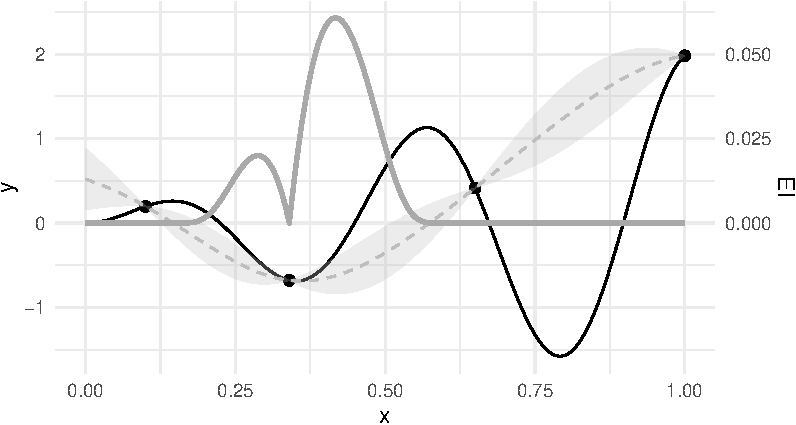
\includegraphics[width=1\textwidth,height=\textheight]{chapters/chapter5/advanced_tuning_methods_and_black_box_optimization_files/figure-pdf/fig-bayesian-optimization-ei-1.pdf}

}

\caption{\label{fig-bayesian-optimization-ei}Expected improvement (solid
dark gray line) based on the mean and uncertainty prediction (dashed
gray line) of the Gaussian process surrogate model trained on an initial
design of four points (black). Ribbons represent the mean plus minus the
standard deviation prediction.}

\end{figure}

We will now proceed to optimize the acquisition function itself to find
the candidate with the largest expected improvement.

\hypertarget{sec-bayesian-optimization-acquisitionopt}{%
\subsubsection{Acquisition Function
Optimizer}\label{sec-bayesian-optimization-acquisitionopt}}

An acquisition function optimizer\index{acquisition function optimizer}
of class
\href{https://mlr3mbo.mlr-org.com/reference/AcqOptimizer.html}{\texttt{AcqOptimizer}}\index{\texttt{AcqOptimizer}}{\marginnote{\begin{footnotesize}\texttt{AcqOptimizer}\end{footnotesize}}}
is used to optimize the acquisition function by efficiently searching
the space of potential candidates within a limited computational budget.

Due to the non-convex nature of most commonly used acquisition functions
(Garnett 2022) it is typical to employ global optimization techniques
for acquisition function optimization. Widely used approaches for
optimizing acquisition functions include derivative-free global
optimization methods like branch and bound algorithms, such as the
DIRECT\index{DIRECT} algorithm (Jones, Perttunen, and Stuckman 1993), as
well as multi-start local optimization methods, such as running the
L-BFGS-B\index{L-BFGS-B} algorithm (Byrd et al. 1995) or a local search
multiple times from various starting points (J. Kim and Choi 2021).
Consequently the optimization problem of the acquisition function can be
handled as a black box optimization problem itself, but a much cheaper
one than the original.

\texttt{AcqOptimizer} objects are constructed with
\href{https://mlr3mbo.mlr-org.com/reference/acqo.html}{\texttt{acqo()}}\index{\texttt{acqo()}}{\marginnote{\begin{footnotesize}\texttt{acqo()}\end{footnotesize}}},
which takes as input a
\href{https://bbotk.mlr-org.com/reference/Optimizer.html}{\texttt{Optimizer}},
a
\href{https://bbotk.mlr-org.com/reference/Terminator.html}{\texttt{Terminator}},
and the acquisition function. Optimizers are stored in the
\href{https://bbotk.mlr-org.com/reference/mlr_optimizers.html}{\texttt{mlr\_optimizers}}
dictionary and can be constructed with the sugar function
\href{https://bbotk.mlr-org.com/reference/opt.html}{\texttt{opt()}}\index{\texttt{opt()}}{\marginnote{\begin{footnotesize}\texttt{opt()}\end{footnotesize}}}.
The terminators are the same as those introduced in
Section~\ref{sec-terminator}.

Below we use the DIRECT algorithm and we terminate the acquisition
function optimization if there is no improvement of at least
\texttt{1e-5} for \texttt{100} iterations. The \texttt{\$optimize()}
method optimizes the acquisition function and returns the next
candidate.

\begin{Shaded}
\begin{Highlighting}[]
\NormalTok{acq\_optimizer }\OtherTok{=} \FunctionTok{acqo}\NormalTok{(}
  \AttributeTok{optimizer =} \FunctionTok{opt}\NormalTok{(}\StringTok{"nloptr"}\NormalTok{, }\AttributeTok{algorithm =} \StringTok{"NLOPT\_GN\_ORIG\_DIRECT"}\NormalTok{),}
  \AttributeTok{terminator =} \FunctionTok{trm}\NormalTok{(}\StringTok{"stagnation"}\NormalTok{, }\AttributeTok{iters =} \DecValTok{100}\NormalTok{, }\AttributeTok{threshold =} \FloatTok{1e{-}5}\NormalTok{),}
  \AttributeTok{acq\_function =}\NormalTok{ acq\_function}
\NormalTok{)}

\NormalTok{candidate }\OtherTok{=}\NormalTok{ acq\_optimizer}\SpecialCharTok{$}\FunctionTok{optimize}\NormalTok{()}
\NormalTok{candidate}
\end{Highlighting}
\end{Shaded}

\begin{verbatim}
        x  x_domain  acq_ei .already_evaluated
1: 0.4173 <list[1]> 0.06074              FALSE
\end{verbatim}

We have now shown how to run a single iteration of the BO algorithm loop
manually. In practice, one would use
\href{https://mlr3mbo.mlr-org.com/reference/mlr_optimizers_mbo.html}{\texttt{OptimizerMbo}}
to put all these pieces together to automate the process. Before
demonstrating this class we will first take a step back and introduce
the \texttt{loop\_function} which tells the algorithm how it should be
run.

\hypertarget{sec-bayesian-optimization-loop}{%
\subsubsection{Using and Building Loop
Functions}\label{sec-bayesian-optimization-loop}}

The
\href{https://mlr3mbo.mlr-org.com/reference/loop_function.html}{\texttt{loop\_function}}\index{\texttt{loop\_function}}
determines the behavior of the BO algorithm on a global level, i.e., how
to define the subroutine that is performed at each iteration to generate
new candidates for evaluation. Loop functions\index{loop functions} are
relatively simple functions that take as input the classes that we have
just discussed and define the BO loop. Loop functions are stored in the
\href{https://mlr3mbo.mlr-org.com/reference/mlr_loop_functions.html}{\texttt{mlr\_loop\_functions}}
dictionary. As these are \texttt{S3} (not \texttt{R6}) classes, they can
be simply loaded by just referencing the \texttt{key} (i.e., there is no
constructor required).

\begin{Shaded}
\begin{Highlighting}[]
\FunctionTok{as.data.table}\NormalTok{(mlr\_loop\_functions)[, .(key, label, instance)]}
\end{Highlighting}
\end{Shaded}

\begin{verbatim}
               key                         label    instance
1:    bayesopt_ego Efficient Global Optimization single-crit
2:    bayesopt_emo           Multi-Objective EGO  multi-crit
3:   bayesopt_mpcl      Multipoint Constant Liar single-crit
4: bayesopt_parego                        ParEGO  multi-crit
5: bayesopt_smsego                       SMS-EGO  multi-crit
\end{verbatim}

You could pick and use one of the loop functions included in the
dictionary above, or you can write your own for finer control over the
BO process. A common choice of loop function is the Efficient Global
Optimization\index{efficient global optimization} (EGO) algorithm
(Jones, Schonlau, and Welch 1998)
(\href{https://mlr3mbo.mlr-org.com/reference/mlr_loop_functions_ego.html}{\texttt{bayesopt\_ego()}}).
A simplified version of this code is shown at the end of this section,
both to help demonstrate the EGO algorithm, and to give an example of
how to write a custom BO variant yourself. In short, the code sets up
the relevant components discussed above and then loops the steps above:
1) update the surrogate model 2) update the acquisition function 3)
optimize the acquisition function to yield a new candidate 4) evaluate
the candidate and add it to the archive. If there is an error during the
loop then a fallback is used where the next candidate is proposed
uniformly at random, ensuring that the process continues even in the
presence of potential issues, we will return to this in
Section~\ref{sec-practical-bayesian-optimization}.

\begin{Shaded}
\begin{Highlighting}[]
\NormalTok{my\_simple\_ego }\OtherTok{=} \ControlFlowTok{function}\NormalTok{(}
\NormalTok{    instance,}
\NormalTok{    surrogate,}
\NormalTok{    acq\_function,}
\NormalTok{    acq\_optimizer,}
\NormalTok{    init\_design\_size}
\NormalTok{  ) \{}

  \CommentTok{\# setting up the building blocks}
\NormalTok{  surrogate}\SpecialCharTok{$}\NormalTok{archive }\OtherTok{=}\NormalTok{ instance}\SpecialCharTok{$}\NormalTok{archive }\CommentTok{\# archive}
\NormalTok{  acq\_function}\SpecialCharTok{$}\NormalTok{surrogate }\OtherTok{=}\NormalTok{ surrogate }\CommentTok{\# surrogate model}
\NormalTok{  acq\_optimizer}\SpecialCharTok{$}\NormalTok{acq\_function }\OtherTok{=}\NormalTok{ acq\_function }\CommentTok{\# acquisition function}

\NormalTok{  search\_space }\OtherTok{=}\NormalTok{ instance}\SpecialCharTok{$}\NormalTok{search\_space}

  \CommentTok{\# initial design}
\NormalTok{  design }\OtherTok{=} \FunctionTok{generate\_design\_sobol}\NormalTok{(}
\NormalTok{    search\_space, }\AttributeTok{n =}\NormalTok{ init\_design\_size)}\SpecialCharTok{$}\NormalTok{data}
\NormalTok{  instance}\SpecialCharTok{$}\FunctionTok{eval\_batch}\NormalTok{(design)}

  \CommentTok{\# MBO loop}
  \ControlFlowTok{repeat}\NormalTok{ \{}
\NormalTok{    candidate }\OtherTok{=} \FunctionTok{tryCatch}\NormalTok{(\{}
      \CommentTok{\# update the surrogate model}
\NormalTok{      acq\_function}\SpecialCharTok{$}\NormalTok{surrogate}\SpecialCharTok{$}\FunctionTok{update}\NormalTok{()}
      \CommentTok{\# update the acquisition function}
\NormalTok{      acq\_function}\SpecialCharTok{$}\FunctionTok{update}\NormalTok{()}
      \CommentTok{\# optimize the acquisition function to yield a new candidate}
\NormalTok{      acq\_optimizer}\SpecialCharTok{$}\FunctionTok{optimize}\NormalTok{()}
\NormalTok{    \}, }\AttributeTok{mbo\_error =} \ControlFlowTok{function}\NormalTok{(mbo\_error\_condition) \{}
      \FunctionTok{generate\_design\_random}\NormalTok{(search\_space, }\AttributeTok{n =}\NormalTok{ 1L)}\SpecialCharTok{$}\NormalTok{data}
\NormalTok{    \})}

    \CommentTok{\# evaluate the candidate and add it to the archive}
    \FunctionTok{tryCatch}\NormalTok{(\{}
\NormalTok{      instance}\SpecialCharTok{$}\FunctionTok{eval\_batch}\NormalTok{(candidate)}
\NormalTok{    \}, }\AttributeTok{terminated\_error =} \ControlFlowTok{function}\NormalTok{(cond) \{}
      \CommentTok{\# $eval\_batch() throws a terminated\_error if the instance is}
      \CommentTok{\# already terminated, e.g. because of timeout.}
\NormalTok{    \})}
    \ControlFlowTok{if}\NormalTok{ (instance}\SpecialCharTok{$}\NormalTok{is\_terminated) }\ControlFlowTok{break}
\NormalTok{  \}}

  \FunctionTok{return}\NormalTok{(instance)}
\NormalTok{\}}
\end{Highlighting}
\end{Shaded}

We are now ready to put everything together to automate the BO process.

\hypertarget{sec-bayesian-black-box-optimization}{%
\subsection{Automating BO with
OptimizerMbo}\label{sec-bayesian-black-box-optimization}}

\href{https://mlr3mbo.mlr-org.com/reference/mlr_optimizers_mbo.html}{\texttt{OptimizerMbo}}
can be used to assemble the building blocks described above into a
single object that can then be used for optimization. We use the
\texttt{bayesopt\_ego} loop function provided by
\texttt{mlr\_loop\_functions}, which works similarly to the code shown
above but takes more care to offer sensible default values for its
arguments and handle edge cases correctly. You do not need to pass any
of these building blocks to each other manually as the
\href{https://bbotk.mlr-org.com/reference/opt.html}{\texttt{opt()}}\index{\texttt{opt()}}{\marginnote{\begin{footnotesize}\texttt{opt()}\end{footnotesize}}}
constructor will do this for you:

\begin{Shaded}
\begin{Highlighting}[]
\NormalTok{bayesopt\_ego }\OtherTok{=}\NormalTok{ mlr\_loop\_functions}\SpecialCharTok{$}\FunctionTok{get}\NormalTok{(}\StringTok{"bayesopt\_ego"}\NormalTok{)}
\NormalTok{surrogate }\OtherTok{=} \FunctionTok{srlrn}\NormalTok{(}\FunctionTok{lrn}\NormalTok{(}\StringTok{"regr.km"}\NormalTok{, }\AttributeTok{covtype =} \StringTok{"matern5\_2"}\NormalTok{,}
  \AttributeTok{optim.method =} \StringTok{"BFGS"}\NormalTok{, }\AttributeTok{control =} \FunctionTok{list}\NormalTok{(}\AttributeTok{trace =} \ConstantTok{FALSE}\NormalTok{)))}
\NormalTok{acq\_function }\OtherTok{=} \FunctionTok{acqf}\NormalTok{(}\StringTok{"ei"}\NormalTok{)}
\NormalTok{acq\_optimizer }\OtherTok{=} \FunctionTok{acqo}\NormalTok{(}\FunctionTok{opt}\NormalTok{(}\StringTok{"nloptr"}\NormalTok{, }\AttributeTok{algorithm =} \StringTok{"NLOPT\_GN\_ORIG\_DIRECT"}\NormalTok{),}
  \AttributeTok{terminator =} \FunctionTok{trm}\NormalTok{(}\StringTok{"stagnation"}\NormalTok{, }\AttributeTok{iters =} \DecValTok{100}\NormalTok{, }\AttributeTok{threshold =} \FloatTok{1e{-}5}\NormalTok{))}

\NormalTok{optimizer }\OtherTok{=} \FunctionTok{opt}\NormalTok{(}\StringTok{"mbo"}\NormalTok{,}
  \AttributeTok{loop\_function =}\NormalTok{ bayesopt\_ego,}
  \AttributeTok{surrogate =}\NormalTok{ surrogate,}
  \AttributeTok{acq\_function =}\NormalTok{ acq\_function,}
  \AttributeTok{acq\_optimizer =}\NormalTok{ acq\_optimizer)}
\end{Highlighting}
\end{Shaded}

\begin{tcolorbox}[enhanced jigsaw, opacitybacktitle=0.6, rightrule=.15mm, opacityback=0, arc=.35mm, breakable, titlerule=0mm, colframe=quarto-callout-tip-color-frame, coltitle=black, bottomrule=.15mm, toprule=.15mm, colback=white, colbacktitle=quarto-callout-tip-color!10!white, bottomtitle=1mm, toptitle=1mm, title=\textcolor{quarto-callout-tip-color}{\faLightbulb}\hspace{0.5em}{Loop Function Arguments}, leftrule=.75mm, left=2mm]

Additional arguments for customizing certain loop functions can be
passed through with the \texttt{args} parameter of \texttt{opt()}.

\end{tcolorbox}

In this example, we will use the same initial design that we created
before and will optimize our sinusoidal function using
\texttt{\$optimize()}:

\begin{Shaded}
\begin{Highlighting}[]
\NormalTok{instance }\OtherTok{=}\NormalTok{ OptimInstanceSingleCrit}\SpecialCharTok{$}\FunctionTok{new}\NormalTok{(objective,}
  \AttributeTok{terminator =} \FunctionTok{trm}\NormalTok{(}\StringTok{"evals"}\NormalTok{, }\AttributeTok{n\_evals =} \DecValTok{20}\NormalTok{))}
\NormalTok{design }\OtherTok{=} \FunctionTok{data.table}\NormalTok{(}\AttributeTok{x =} \FunctionTok{c}\NormalTok{(}\FloatTok{0.1}\NormalTok{, }\FloatTok{0.34}\NormalTok{, }\FloatTok{0.65}\NormalTok{, }\DecValTok{1}\NormalTok{))}
\NormalTok{instance}\SpecialCharTok{$}\FunctionTok{eval\_batch}\NormalTok{(design)}
\NormalTok{optimizer}\SpecialCharTok{$}\FunctionTok{optimize}\NormalTok{(instance)}
\end{Highlighting}
\end{Shaded}

\begin{verbatim}
        x  x_domain      y
1: 0.7922 <list[1]> -1.577
\end{verbatim}

Using only a few evaluations, BO comes close to the true global optimum
(0.792). Figure~\ref{fig-bayesian-optimization-sampling} shows the
sampling trajectory of candidates as the algorithm progressed, we can
see that focus is increasingly given to more regions around the global
optimum. However, even in later optimization stages, the algorithm still
explores new areas, illustrating that the expected improvement
acquisition function indeed balances exploration and exploitation as we
required.

\begin{figure}

{\centering 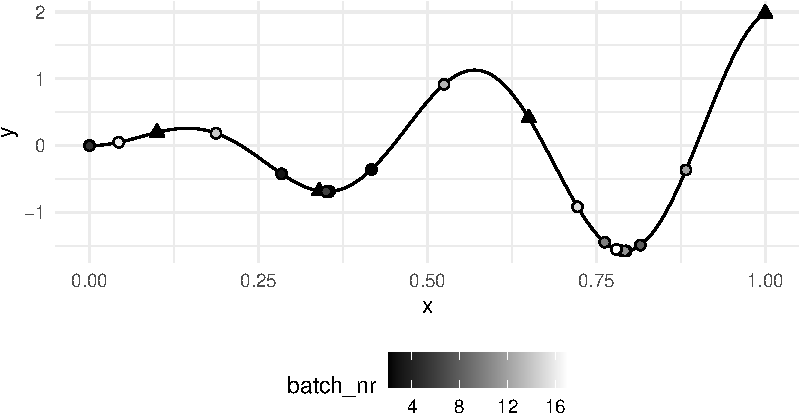
\includegraphics[width=1\textwidth,height=\textheight]{chapters/chapter5/advanced_tuning_methods_and_black_box_optimization_files/figure-pdf/fig-bayesian-optimization-sampling-1.pdf}

}

\caption{\label{fig-bayesian-optimization-sampling}Sampling trajectory
of the BO algorithm. Points of the initial design in black triangles.
Sampled points are in dots with color progressing from black to white as
the algorithm progresses.}

\end{figure}

If we replicate running our BO algorithm ten times (with random initial
designs and varying random seeds) and compare this to a random search,
we can see that BO indeed performs much better and on average reaches
the global optimum after around 15 function evaluations
(Figure~\ref{fig-bayesian-sinusoidal_bo_rs}). As expected, the
performance for the initial design size is close to the performance of
the random search.

\begin{figure}

{\centering 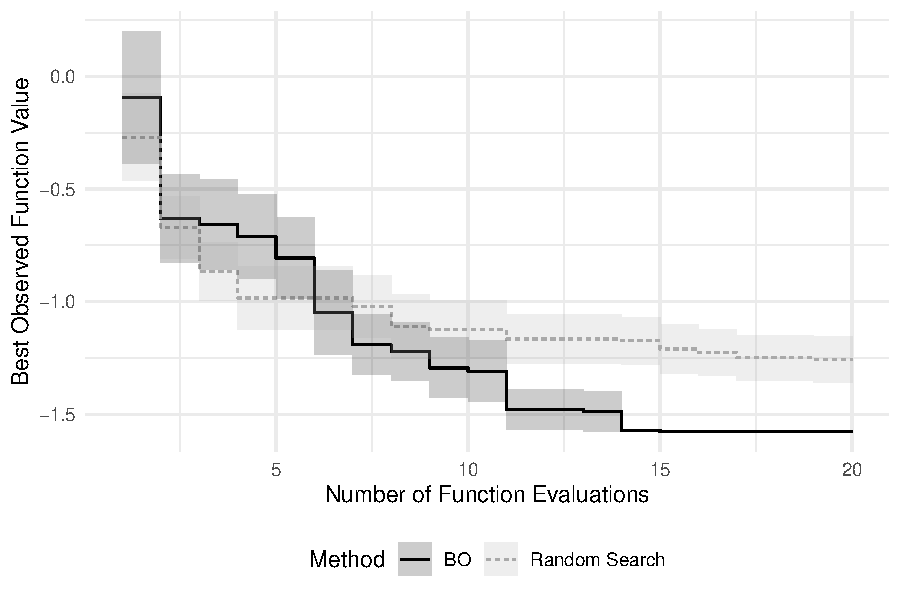
\includegraphics[width=1\textwidth,height=\textheight]{chapters/chapter5/Figures/bo_1d_sinusoidal_bo_rs.pdf}

}

\caption{\label{fig-bayesian-sinusoidal_bo_rs}Anytime performance of BO
and random search on the 1D sinusoidal function given a budget of 20
function evaluations. Solid line depicts the best observed target value
averaged over 10 replications. Ribbons represent standard errors.}

\end{figure}

\hypertarget{sec-bayesian-tuning}{%
\subsection{Bayesian Optimization for HPO}\label{sec-bayesian-tuning}}

\texttt{mlr3mbo} can be used for HPO by making use of
\href{https://mlr3mbo.mlr-org.com/reference/mlr_tuners_mbo.html}{\texttt{TunerMbo}}\index{\texttt{TunerMbo}}{\marginnote{\begin{footnotesize}\texttt{TunerMbo}\end{footnotesize}}},
which is a wrapper around
\href{https://mlr3mbo.mlr-org.com/reference/mlr_optimizers_mbo.html}{\texttt{OptimizerMbo}}
and works in the exact same way. As an example, below we will tune the
\texttt{cost} and \texttt{gamma} parameters of
\texttt{lrn("classif.svm")} with a radial kernel on
\texttt{tsk("sonar")} with three-fold CV. We set up \texttt{tnr("mbo")}
using the same objects constructed above and then run our tuning
experiment as usual:

\begin{Shaded}
\begin{Highlighting}[]
\NormalTok{tuner }\OtherTok{=} \FunctionTok{tnr}\NormalTok{(}\StringTok{"mbo"}\NormalTok{,}
  \AttributeTok{loop\_function =}\NormalTok{ bayesopt\_ego,}
  \AttributeTok{surrogate =}\NormalTok{ surrogate,}
  \AttributeTok{acq\_function =}\NormalTok{ acq\_function,}
  \AttributeTok{acq\_optimizer =}\NormalTok{ acq\_optimizer)}

\NormalTok{lrn\_svm }\OtherTok{=} \FunctionTok{lrn}\NormalTok{(}\StringTok{"classif.svm"}\NormalTok{, }\AttributeTok{kernel =} \StringTok{"radial"}\NormalTok{,}
  \AttributeTok{type =} \StringTok{"C{-}classification"}\NormalTok{,}
  \AttributeTok{cost  =} \FunctionTok{to\_tune}\NormalTok{(}\FloatTok{1e{-}5}\NormalTok{, }\FloatTok{1e5}\NormalTok{, }\AttributeTok{logscale =} \ConstantTok{TRUE}\NormalTok{),}
  \AttributeTok{gamma =} \FunctionTok{to\_tune}\NormalTok{(}\FloatTok{1e{-}5}\NormalTok{, }\FloatTok{1e5}\NormalTok{, }\AttributeTok{logscale =} \ConstantTok{TRUE}\NormalTok{)}
\NormalTok{)}

\NormalTok{instance }\OtherTok{=} \FunctionTok{tune}\NormalTok{(tuner, }\FunctionTok{tsk}\NormalTok{(}\StringTok{"sonar"}\NormalTok{), lrn\_svm, }\FunctionTok{rsmp}\NormalTok{(}\StringTok{"cv"}\NormalTok{, }\AttributeTok{folds =} \DecValTok{3}\NormalTok{),}
  \FunctionTok{msr}\NormalTok{(}\StringTok{"classif.ce"}\NormalTok{), }\DecValTok{25}\NormalTok{)}

\NormalTok{instance}\SpecialCharTok{$}\NormalTok{result}
\end{Highlighting}
\end{Shaded}

\begin{verbatim}
    cost  gamma learner_param_vals  x_domain classif.ce
1: 11.51 -4.075          <list[4]> <list[2]>     0.1489
\end{verbatim}

Multi-objective tuning is also possible with BO with algorithms using
many different design choices, for example, whether they use a
scalarization approach of objectives and only rely on a single surrogate
model, or fit a surrogate model for each objective. More details on
multi-objective BO can for example be found in Horn et al. (2015) or
Morales-Hernández, Van Nieuwenhuyse, and Rojas Gonzalez (2022).

Below we will illustrate multi-objective tuning using the ParEGO
(Knowles 2006) loop function. ParEGO
(\href{https://mlr3mbo.mlr-org.com/reference/mlr_loop_functions_parego.html}{\texttt{bayesopt\_parego()}})
tackles multi-objective BO via a randomized scalarization approach and
models a single scalarized objective function via a single surrogate
model and then proceeds to find the next candidate for evaluation making
use of a standard single-objective acquisition function such as the
expected improvement. Other compatible loop functions can be found by
looking at the \texttt{"instance"} column of
\href{https://mlr3mbo.mlr-org.com/reference/mlr_loop_functions.html}{\texttt{mlr\_loop\_functions}}.
We will tune three parameters of a decision tree with respect to the
true positive (maximize) and false positive (minimize) rates, the Pareto
front\index{Pareto front} is visualized in
Figure~\ref{fig-pareto-bayesopt}.

\begin{Shaded}
\begin{Highlighting}[]
\NormalTok{tuner }\OtherTok{=} \FunctionTok{tnr}\NormalTok{(}\StringTok{"mbo"}\NormalTok{,}
  \AttributeTok{loop\_function =}\NormalTok{ bayesopt\_parego,}
  \AttributeTok{surrogate =}\NormalTok{ surrogate,}
  \AttributeTok{acq\_function =}\NormalTok{ acq\_function,}
  \AttributeTok{acq\_optimizer =}\NormalTok{ acq\_optimizer)}

\NormalTok{lrn\_rpart }\OtherTok{=} \FunctionTok{lrn}\NormalTok{(}\StringTok{"classif.rpart"}\NormalTok{,}
  \AttributeTok{cp =} \FunctionTok{to\_tune}\NormalTok{(}\FloatTok{1e{-}04}\NormalTok{, }\FloatTok{1e{-}1}\NormalTok{),}
  \AttributeTok{minsplit =} \FunctionTok{to\_tune}\NormalTok{(}\DecValTok{2}\NormalTok{, }\DecValTok{64}\NormalTok{),}
  \AttributeTok{maxdepth =} \FunctionTok{to\_tune}\NormalTok{(}\DecValTok{1}\NormalTok{, }\DecValTok{30}\NormalTok{)}
\NormalTok{)}

\NormalTok{instance }\OtherTok{=} \FunctionTok{tune}\NormalTok{(tuner, }\FunctionTok{tsk}\NormalTok{(}\StringTok{"sonar"}\NormalTok{), lrn\_svm, }\FunctionTok{rsmp}\NormalTok{(}\StringTok{"cv"}\NormalTok{, }\AttributeTok{folds =} \DecValTok{3}\NormalTok{),}
  \FunctionTok{msrs}\NormalTok{(}\FunctionTok{c}\NormalTok{(}\StringTok{"classif.tpr"}\NormalTok{, }\StringTok{"classif.fpr"}\NormalTok{)), }\DecValTok{25}\NormalTok{)}
\end{Highlighting}
\end{Shaded}

\begin{figure}

{\centering 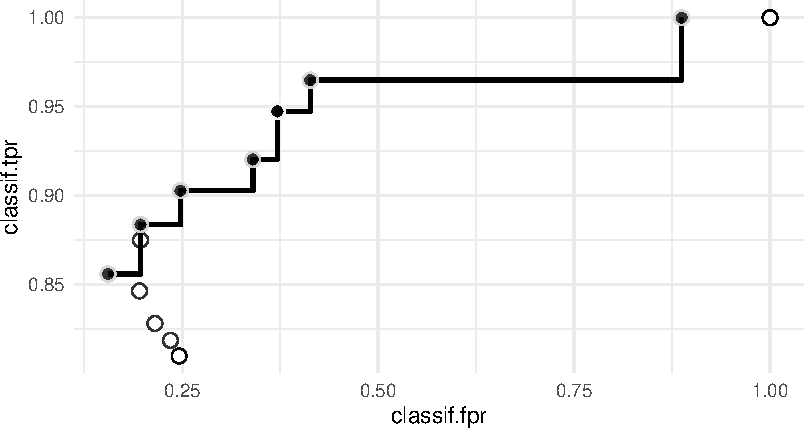
\includegraphics[width=1\textwidth,height=\textheight]{chapters/chapter5/advanced_tuning_methods_and_black_box_optimization_files/figure-pdf/fig-pareto-bayesopt-1.pdf}

}

\caption{\label{fig-pareto-bayesopt}Pareto front of TPR and FPR obtained
via ParEGO. White dots represent tested configurations, each black dot
individually represents a Pareto-optimal configuration and all black
dots together represent the Pareto front.}

\end{figure}

\hypertarget{sec-noisy-bayesian-optimization}{%
\subsection{Noisy Bayesian
Optimization}\label{sec-noisy-bayesian-optimization}}

So far, we implicitly assumed that the black box function we are trying
to optimize is deterministic, i.e., repeatedly evaluating the same point
will always return the same objective function value. However,
real-world black box functions are often noisy, which means that
repeatedly evaluating the same point will return different objective
function values due to background noise on top of the black box
function. For example, if you were modeling a machine in a factory to
estimate the rate of production, even if all parameters of the machine
were controlled, we would still expect different performance at
different times due to uncontrollable background factors such as
environmental conditions.

In \texttt{bbotk}, you can mark an
\href{https://bbotk.mlr-org.com/reference/Objective.html}{\texttt{Objective}}
object as noisy by passing the \texttt{"noisy"} tag to the
\texttt{properties} parameter, which allows us to use methods that can
treat such objectives differently.

\begin{Shaded}
\begin{Highlighting}[]
\NormalTok{sinus\_1D\_noisy }\OtherTok{=} \ControlFlowTok{function}\NormalTok{(xs) \{}
\NormalTok{  y }\OtherTok{=} \DecValTok{2} \SpecialCharTok{*}\NormalTok{ xs}\SpecialCharTok{$}\NormalTok{x }\SpecialCharTok{*} \FunctionTok{sin}\NormalTok{(}\DecValTok{14} \SpecialCharTok{*}\NormalTok{ xs}\SpecialCharTok{$}\NormalTok{x) }\SpecialCharTok{+} \FunctionTok{rnorm}\NormalTok{(}\DecValTok{1}\NormalTok{, }\AttributeTok{mean =} \DecValTok{0}\NormalTok{, }\AttributeTok{sd =} \FloatTok{0.1}\NormalTok{)}
\NormalTok{  y}
\NormalTok{\}}
\NormalTok{domain }\OtherTok{=} \FunctionTok{ps}\NormalTok{(}\AttributeTok{x =} \FunctionTok{p\_dbl}\NormalTok{(}\AttributeTok{lower =} \DecValTok{0}\NormalTok{, }\AttributeTok{upper =} \DecValTok{1}\NormalTok{))}
\NormalTok{codomain }\OtherTok{=} \FunctionTok{ps}\NormalTok{(}\AttributeTok{y =} \FunctionTok{p\_dbl}\NormalTok{(}\AttributeTok{tags =} \StringTok{"minimize"}\NormalTok{))}
\NormalTok{objective\_noisy }\OtherTok{=}\NormalTok{ ObjectiveRFun}\SpecialCharTok{$}\FunctionTok{new}\NormalTok{(sinus\_1D\_noisy,}
  \AttributeTok{domain =}\NormalTok{ domain, }\AttributeTok{codomain =}\NormalTok{ codomain, }\AttributeTok{properties =} \StringTok{"noisy"}\NormalTok{)}
\end{Highlighting}
\end{Shaded}

Noisy objectives can be treated in different ways:

\begin{enumerate}
\def\labelenumi{\arabic{enumi}.}
\tightlist
\item
  A surrogate model can be used to incorporate the noise
\item
  An acquisition function can be used that respects noisiness
\item
  The final best point(s) after optimization (i.e., the
  \texttt{\$result} field of the instance) can be chosen in a way to
  reflect noisiness
\end{enumerate}

In the first case, instead of using an interpolating Gaussian
process\index{Gaussian process}, we could instead use Gaussian process
regression that estimates the measurement error by setting
\texttt{nugget.estim\ =\ TRUE}:

\begin{Shaded}
\begin{Highlighting}[]
\FunctionTok{srlrn}\NormalTok{(}\FunctionTok{lrn}\NormalTok{(}\StringTok{"regr.km"}\NormalTok{, }\AttributeTok{nugget.estim =} \ConstantTok{TRUE}\NormalTok{))}
\end{Highlighting}
\end{Shaded}

This will result in the Gaussian process not perfectly interpolating
training data and the standard deviation prediction associated with the
training data will be non-zero, reflecting the uncertainty in the
observed function values due to the measurement error. A more in-depth
discussion of noise-free vs.~noisy observations in the context of
Gaussian processes can be found in Chapter 2 of Williams and Rasmussen
(2006).

For the second option, one example of an acquisition function that
respects noisiness is the Augmented expected improvement (D. Huang et
al. 2012) (\texttt{acqf("aei")}) which essentially rescales the expected
improvement, taking measurement error into account.

Finally, \texttt{mlr3mbo} allows for explicitly specifying how the final
result after optimization is assigned to the instance (i.e., what will
be saved in \texttt{instance\$result}) with a result
assigner\index{result assigner}{\marginnote{\begin{footnotesize}Result
Assigner\end{footnotesize}}}, which can be specified during the
construction of an \texttt{OptimizerMbo} or \texttt{TunerMbo}.
\href{https://mlr3mbo.mlr-org.com/reference/mlr_result_assigners_surrogate.html}{\texttt{ResultAssignerSurrogate}}
uses a surrogate model to predict the mean of all evaluated points and
proceeds to choose the point with the best mean prediction as the final
optimization result. In contrast, the default method,
\href{https://mlr3mbo.mlr-org.com/reference/mlr_result_assigners_archive.html}{\texttt{ResultAssignerArchive}},
just picks the best point according to the evaluations logged in
\texttt{archive}. Result assigners are stored in the
\href{https://mlr3mbo.mlr-org.com/reference/mlr_result_assigners.html}{\texttt{mlr\_result\_assigners}}
dictionary and can be constructed with
\href{https://mlr3mbo.mlr-org.com/reference/ras.html}{\texttt{ras()}}.

\begin{Shaded}
\begin{Highlighting}[]
\FunctionTok{opt}\NormalTok{(}\StringTok{"mbo"}\NormalTok{,}
  \AttributeTok{loop\_function =}\NormalTok{ bayesopt\_ego,}
  \AttributeTok{surrogate =}\NormalTok{ surrogate,}
  \AttributeTok{acq\_function =}\NormalTok{ acq\_function,}
  \AttributeTok{acq\_optimizer =}\NormalTok{ acq\_optimizer,}
  \AttributeTok{result\_assigner =} \FunctionTok{ras}\NormalTok{(}\StringTok{"surrogate"}\NormalTok{)}
\NormalTok{)}
\end{Highlighting}
\end{Shaded}

\hypertarget{sec-practical-bayesian-optimization}{%
\subsection{Practical Considerations in Bayesian
Optimization}\label{sec-practical-bayesian-optimization}}

\texttt{mlr3mbo} tries to use reasonable defaults regarding the choice
of surrogate model, acquisition function, acquisition function optimizer
and even the loop function. For example, in the case of a purely numeric
search space, \texttt{mlr3mbo} will by default use a Gaussian process as
the surrogate model and a random forest as the fallback learner and
additionally encapsulates the learner
(Section~\ref{sec-encapsulation-fallback}). In the case of a mixed or
hierarchical search space, \texttt{mlr3mbo} will use a random forest as
the surrogate model. Therefore, users can perform BO without specifying
any deviation from the defaults and still expect decent optimization
performance. To see an up-to-date overview of these defaults, take a
look at the help page of
\href{https://mlr3mbo.mlr-org.com/reference/mbo_defaults.html}{\texttt{mbo\_defaults}}.
We will finish this section with some practical considerations to think
about when using BO.

\hypertarget{error-handling}{%
\subsubsection*{Error Handling}\label{error-handling}}

In the context of BO, there is plenty of room for potential failure of
building blocks which could break the whole process. For example, if two
points in the training data are too close to each other, fitting the
Gaussian process surrogate model can fail.

\texttt{mlr3mbo} has several built-in safety nets to catch errors.
\href{https://mlr3mbo.mlr-org.com/reference/Surrogate.html}{\texttt{Surrogate}}
includes the \texttt{catch\_errors} configuration control parameter,
which, if set to \texttt{TRUE}, catches all errors that occur during
training or updating of the surrogate model.
\href{https://mlr3mbo.mlr-org.com/reference/AcqOptimizer.html}{\texttt{AcqOptimizer}}
also has the \texttt{catch\_errors} configuration control parameter,
which can be used to catch all errors that occur during the acquisition
function optimization, either due to the surrogate model failing to
predict or the acquisition function optimizer erroring. If errors are
caught in any of these steps, the standard behavior of any
\href{https://mlr3mbo.mlr-org.com/reference/loop_function.html}{\texttt{loop\_function}}
is to trigger a fallback, which proposes the next candidate uniformly at
random. Note, when setting \texttt{catch\_errors\ =\ TRUE} for the
\href{https://mlr3mbo.mlr-org.com/reference/AcqOptimizer.html}{\texttt{AcqOptimizer}},
it is usually not necessary to also explicitly set
\texttt{catch\_errors\ =\ TRUE} for the \texttt{Surrogate}, though this
may be useful when debugging.

In the worst-case scenario, if all iterations errored, the BO algorithm
will simply perform a random search. Ideally, fallback learners
(Section~\ref{sec-encapsulation-fallback}) should also be used, which
will be employed before proposing the next candidate randomly. The value
of the acquisition function is also always logged in the archive of the
optimization instance so inspecting this is a good idea to ensure the
algorithm behaved as expected.

\hypertarget{surrogate-models}{%
\subsubsection*{Surrogate Models}\label{surrogate-models}}

In practice, users may prefer a more robust BO variant over a
potentially better-performing but unstable variant. Even if the
\texttt{catch\_errors} parameters are turned on and are never triggered,
that does not guarantee that the BO algorithm ran as intended. For
instance, Gaussian processes are sensitive to the choice of kernel and
kernel parameters, typically estimated through maximum likelihood
estimation, suboptimal parameter values can result in white noise models
with a constant mean and standard deviation prediction. In this case,
the surrogate model will not provide useful mean and standard deviation
predictions resulting in poor overall performance of the BO algorithm.
Another practical consideration regarding the choice of surrogate model
can be overhead. Fitting a vanilla Gaussian process scales cubically in
the number of data points and therefore the overhead of the BO algorithm
grows with the number of iterations. Furthermore, vanilla Gaussian
processes natively cannot handle categorical input variables or
dependencies in the search space (recall that in HPO we often deal with
mixed hierarchical spaces). In contrast, a random forest -- popularly
used as a surrogate model in \emph{SMAC} (Lindauer et al. 2022) -- is
cheap to train, quite robust in the sense that it is not as sensitive to
its hyperparameters as a Gaussian process, and can easily handle mixed
hierarchical spaces. On the downside, a random forest is not really
Bayesian (i.e., there is no posterior predictive distribution) and
suffers from poor uncertainty estimates and poor extrapolation.

\hypertarget{warmstarting}{%
\subsubsection*{Warmstarting}\label{warmstarting}}

Warmstarting is a technique in optimization where previous optimization
runs are used to improve the convergence rate and final solution of a
new, related optimization run. In BO, warmstarting can be achieved by
providing a set of likely well-performing configurations as part of the
initial design (see, e.g., Feurer, Springenberg, and Hutter 2015). This
approach can be particularly advantageous because it allows the
surrogate model to start with prior knowledge of the optimization
landscape in relevant regions. In \texttt{mlr3mbo}, warmstarting is
straightforward by specifying a custom initial design. Furthermore, a
convenient feature of \texttt{mlr3mbo} is the ability to continue
optimization in an online fashion even after an optimization run has
been terminated. Both
\href{https://mlr3mbo.mlr-org.com/reference/mlr_optimizers_mbo.html}{\texttt{OptimizerMbo}}
and
\href{https://mlr3mbo.mlr-org.com/reference/mlr_tuners_mbo.html}{\texttt{TunerMbo}}
support this feature, allowing optimization to resume on a given
instance even if the optimization was previously interrupted or
terminated.

\hypertarget{termination}{%
\subsubsection*{Termination}\label{termination}}

Common termination criteria include stopping after a fixed number of
evaluations, once a given walltime budget has been reached, when
performance reaches a certain level, or when performance improvement
stagnates. In the context of BO, it can also be sensible to stop the
optimization if the best acquisition function value falls below a
certain threshold. For instance, terminating the optimization if the
expected improvement of the next candidate(s) is negligible can be a
reasonable approach. At the time of publishing, terminators based on
acquisition functions have not been implemented but this feature will be
coming soon.

\hypertarget{parallelization}{%
\subsubsection*{Parallelization}\label{parallelization}}

The standard behavior of most BO algorithms is to sequentially propose a
single candidate that should be evaluated next. Users may want to use
parallelization to compute candidates more efficiently. If you are using
BO for HPO, then the most efficient method is to parallelize the nested
resampling, see Section~\ref{sec-nested-resampling-parallelization}.
Alternatively, if the loop function supports candidates being proposed
in batches (e.g., \texttt{bayesopt\_parego()}) then the \texttt{q}
argument to the loop function can be set to propose \texttt{q}
candidates in each iteration that can be evaluated in parallel if the
\texttt{Objective} is properly implemented.

\hypertarget{conclusion-3}{%
\section{Conclusion}\label{conclusion-3}}

In this chapter, we looked at advanced tuning methods. We started by
thinking about the types of errors that can occur during tuning and how
to handle these to ensure your HPO process does not crash. We presented
multi-objective tuning, which can be used to optimize performance
measures simultaneously. We then looked at multi-fidelity tuning, in
which the Hyberband tuner can be used to efficiently tune algorithms by
making use of lower-fidelity evaluations to approximate full-fidelity
model performance. We will return to Hyperband in
Section~\ref{sec-hyperband-example-svm} where we will learn how to make
use of pipelines in order to tune any algorithm with Hyperband. Finally,
we took a deep dive into Bayesian optimization to look at how
\href{https://bbotk.mlr-org.com}{\texttt{bbotk}}\index{\texttt{bbotk}},
\href{https://mlr3mbo.mlr-org.com}{\texttt{mlr3mbo}}\index{\texttt{mlr3mbo}},
and
\href{https://mlr3tuning.mlr-org.com}{\texttt{mlr3tuning}}\index{\texttt{mlr3tuning}}
can be used together to implement complex BO tuning algorithms in
\texttt{mlr3}, allowing for highly flexible and sample-efficient
algorithms. In the next chapter we will look at feature selection and
see how
\href{https://mlr3filters.mlr-org.com}{\texttt{mlr3filters}}\index{\texttt{mlr3filters}}
and
\href{https://mlr3fselect.mlr-org.com}{\texttt{mlr3fselect}}\index{\texttt{mlr3fselect}}
use a very similar design interface to \texttt{mlr3tuning}.

\hypertarget{tbl-api-advanced-tuning}{}
\begin{longtable}[]{@{}
  >{\raggedright\arraybackslash}p{(\columnwidth - 4\tabcolsep) * \real{0.4444}}
  >{\raggedright\arraybackslash}p{(\columnwidth - 4\tabcolsep) * \real{0.3333}}
  >{\raggedright\arraybackslash}p{(\columnwidth - 4\tabcolsep) * \real{0.2222}}@{}}
\caption{\label{tbl-api-advanced-tuning}Important classes and functions
covered in this chapter with underlying class (if applicable), class
constructor or function, and important class methods (if
applicable).}\tabularnewline
\toprule\noalign{}
\begin{minipage}[b]{\linewidth}\raggedright
Class
\end{minipage} & \begin{minipage}[b]{\linewidth}\raggedright
Constructor/Function
\end{minipage} & \begin{minipage}[b]{\linewidth}\raggedright
Fields/Methods
\end{minipage} \\
\midrule\noalign{}
\endfirsthead
\toprule\noalign{}
\begin{minipage}[b]{\linewidth}\raggedright
Class
\end{minipage} & \begin{minipage}[b]{\linewidth}\raggedright
Constructor/Function
\end{minipage} & \begin{minipage}[b]{\linewidth}\raggedright
Fields/Methods
\end{minipage} \\
\midrule\noalign{}
\endhead
\bottomrule\noalign{}
\endlastfoot
\href{https://mlr3.mlr-org.com/reference/Learner.html}{\texttt{Learner}}
& \href{https://mlr3.mlr-org.com/reference/mlr_sugar.html}{\texttt{lrn}}
& \texttt{\$encapsulate}; \texttt{\$fallback} \\
\href{https://mlr3tuning.mlr-org.com/reference/TuningInstanceMultiCrit.html}{\texttt{TuningInstanceMultiCrit}}
&
\href{https://mlr3tuning.mlr-org.com/reference/ti.html}{\texttt{ti()}}/\href{https://mlr3tuning.mlr-org.com/reference/tune.html}{\texttt{tune()}}
& \texttt{\$result}; \texttt{\$archive} \\
\href{https://mlr3hyperband.mlr-org.com/reference/TunerHyperband.html}{\texttt{TunerHyperband}}
& \texttt{tnr("hyperband")} & - \\
\href{https://bbotk.mlr-org.com/reference/Objective.html}{\texttt{Objective}}
& - & \\
\href{https://bbotk.mlr-org.com/reference/OptimInstanceSingleCrit.html}{\texttt{OptimInstanceSingleCrit}}
or
\href{https://bbotk.mlr-org.com/reference/OptimInstanceMultiCrit.html}{\texttt{OptimInstanceMultiCrit}}
&
\href{https://bbotk.mlr-org.com/reference/bb_optimize.html}{\texttt{bb\_optimize()}}
& \texttt{\$result}; \texttt{\$archive} \\
\href{https://mlr3mbo.mlr-org.com/reference/SurrogateLearner.html}{\texttt{SurrogateLearner}}
&
\href{https://mlr3mbo.mlr-org.com/reference/srlrn.html}{\texttt{srlrn()}}
& \\
\href{https://mlr3mbo.mlr-org.com/reference/AcqFunction.html}{\texttt{AcqFunction}}
&
\href{https://mlr3mbo.mlr-org.com/reference/acqf.html}{\texttt{acqf()}}
& \\
\href{https://mlr3mbo.mlr-org.com/reference/AcqOptimizer.html}{\texttt{AcqOptimizer}}
&
\href{https://mlr3mbo.mlr-org.com/reference/acqo.html}{\texttt{acqo()}}
& \\
- &
\href{https://mlr3mbo.mlr-org.com/reference/loop_function.html}{\texttt{loop\_function}}
& - \\
\href{https://mlr3mbo.mlr-org.com/reference/mlr_optimizers_mbo.html}{\texttt{OptimizerMbo}}
& \texttt{bbotk::opt("mbo")} & \\
\href{https://mlr3mbo.mlr-org.com/reference/mlr_tuners_mbo.html}{\texttt{TunerMbo}}
& \texttt{tnr("mbo")} & \\
\href{https://paradox.mlr-org.com/reference/Design.html}{\texttt{Design}}
&
\href{https://paradox.mlr-org.com/reference/generate_design_random.html}{\texttt{generate\_design\_random}};
\href{https://paradox.mlr-org.com/reference/generate_design_grid.html}{\texttt{generate\_design\_grid}};
\href{https://paradox.mlr-org.com/reference/generate_design_lhs.html}{\texttt{generate\_design\_lhs}};
\href{https://paradox.mlr-org.com/reference/generate_design_sobol.html}{\texttt{generate\_design\_sobol}};
& \texttt{\$data} \\
\end{longtable}

\hypertarget{exercises-3}{%
\section{Exercises}\label{exercises-3}}

\begin{enumerate}
\def\labelenumi{\arabic{enumi}.}
\tightlist
\item
  Tune the \texttt{mtry}, \texttt{sample.fraction}, and
  \texttt{num.trees} hyperparameters of \texttt{lrn("regr.ranger")} on
  \texttt{tsk("mtcars")} and evaluate this with a three-fold CV and the
  root mean squared error (same as Chapter~\ref{sec-optimization},
  Exercise 1). Use \texttt{tnr("mbo")} with 50 evaluations. Compare this
  with the performance progress of a random search run from
  Chapter~\ref{sec-optimization}, Exercise 1. Plot the progress of
  performance over iterations and visualize the spatial distribution of
  the evaluated hyperparameter configurations for both algorithms.
\item
  Minimize the 2D Rastrigin function
  \(f: [-5.12, 5.12] \times [-5.12, 5.12] \rightarrow \mathbb{R}\),
  \(\mathbf{x} \mapsto 10 D+\sum_{i=1}^D\left[x_i^2-10 \cos \left(2 \pi x_i\right)\right]\),
  \(D = 2\) via BO (standard sequential single-objective BO via
  \texttt{bayesopt\_ego()}) using the lower confidence bound with
  \texttt{lambda\ =\ 1} as acquisition function and
  \texttt{"NLOPT\_GN\_ORIG\_DIRECT"} via \texttt{opt("nloptr")} as
  acquisition function optimizer. Use a budget of 40 function
  evaluations. Run this with both the ``default'' Gaussian process
  surrogate model with Matérn 5/2 kernel, and the ``default'' random
  forest surrogate model. Compare their anytime performance (similarly
  as in Figure~\ref{fig-bayesian-sinusoidal_bo_rs}). You can construct
  the surrogate models with default settings using:
\end{enumerate}

\begin{Shaded}
\begin{Highlighting}[]
\NormalTok{surrogate\_gp }\OtherTok{=} \FunctionTok{srlrn}\NormalTok{(}\FunctionTok{default\_gp}\NormalTok{())}
\NormalTok{surrogate\_rf }\OtherTok{=} \FunctionTok{srlrn}\NormalTok{(}\FunctionTok{default\_rf}\NormalTok{())}
\end{Highlighting}
\end{Shaded}

\begin{enumerate}
\def\labelenumi{\arabic{enumi}.}
\setcounter{enumi}{2}
\tightlist
\item
  Minimize the following function:
  \(f: [-10, 10] \rightarrow \mathbb{R}^2, x \mapsto \left(x^2, (x - 2)^2\right)\)
  with respect to both objectives. Use the ParEGO algorithm. Construct
  the objective function using the
  \href{https://bbotk.mlr-org.com/reference/ObjectiveRFunMany.html}{\texttt{ObjectiveRFunMany}}
  class. Terminate the optimization after a runtime of 100 evals. Plot
  the resulting Pareto front and compare it to the analytical solution,
  \(y_2 = \left(\sqrt{y_1}-2\right)^2\) with \(y_1\) ranging from \(0\)
  to \(4\).
\end{enumerate}

\hypertarget{sec-feature-selection}{%
\chapter{Feature Selection}\label{sec-feature-selection}}

\vspace{-15mm}\addtocontents{toc}{\textit{Marvin N. Wright}}

\textbf{Marvin N. Wright} \newline  \emph{Leibniz Institute for
Prevention Research and Epidemiology -- BIPS, and University of Bremen,
and University of Copenhagen} \newline \newline 

Feature selection\index{feature selection}, also known as variable or
descriptor
selection\index{variable selection|see{feature selection}}\index{descriptor selection|see{feature selection}},
is the process of finding a subset of features to use with a given task
and learner. Using an \emph{optimal set} of features can have several
benefits:

\begin{itemize}
\tightlist
\item
  improved predictive performance, since we reduce overfitting on
  irrelevant features,
\item
  robust models that do not rely on noisy features,
\item
  simpler models that are easier to interpret,
\item
  faster model fitting, e.g.~for model updates,
\item
  faster prediction, and
\item
  no need to collect potentially expensive features.
\end{itemize}

However, these objectives will not necessarily be optimized by the same
set of features and thus feature selection can be seen as a
multi-objective optimization\index{multi-objective optimization}
problem. In this chapter, we mostly focus on feature selection as a
means of improving predictive performance, but also briefly cover the
optimization of multiple criteria (Section~\ref{sec-multicrit-featsel}).

Reducing the number of features can improve models across many
scenarios, but it can be especially helpful in datasets that have a high
number of features in comparison to the number of data points. Many
learners perform implicit, also called embedded, feature
selection,\index{feature selection!implicit}\index{feature selection!embedded}
e.g.~via the choice of variables used for splitting in a decision tree.
Most other feature selection methods are model agnostic, i.e.~they can
be used together with any learner. Of the many different approaches to
identifying relevant features, we will focus on two general concepts,
which are described in detail below: Filter and Wrapper methods (Guyon
and Elisseeff 2003; Chandrashekar and Sahin 2014).

\hypertarget{sec-fs-filter}{%
\section{Filters}\label{sec-fs-filter}}

Filter methods are preprocessing\index{preprocessing} steps that can be
applied before training a model. A very simple filter approach could
look like this:

\begin{enumerate}
\def\labelenumi{\arabic{enumi}.}
\tightlist
\item
  calculate the correlation coefficient \(\rho\) between each feature
  and a numeric target variable, and
\item
  select all features with \(\rho > 0.2\) for further modeling steps.
\end{enumerate}

This approach is a \emph{univariate} filter because it only considers
the univariate relationship between each feature and the target
variable. Further, it can only be applied to regression tasks with
continuous features and the threshold of \(\rho > 0.2\) is quite
arbitrary. Thus, more advanced filter methods, e.g.~\emph{multivariate}
filters based on feature importance, usually perform better (Bommert et
al. 2020). On the other hand, a benefit of univariate filters is that
they are usually computationally cheaper than more complex filter or
wrapper methods. In the following, we describe how to calculate
univariate, multivariate and feature importance filters, how to access
implicitly selected features, how to integrate filters in a machine
learning pipeline and how to optimize filter thresholds.

Filter algorithms select features by assigning numeric scores to each
feature, e.g.~correlation between features and target variable, use
these to rank the features and select a feature subset based on the
ranking. Features that are assigned lower scores are then omitted in
subsequent modeling steps. All filters are implemented via the package
\href{https://mlr3filters.mlr-org.com}{\texttt{mlr3filters}}\index{\texttt{mlr3filters}}.
Below, we cover how to

\begin{itemize}
\tightlist
\item
  instantiate a
  \href{https://www.rdocumentation.org/packages/base/topics/funprog}{\texttt{Filter}}
  object,
\item
  calculate scores for a given task, and
\item
  use calculated scores to select or drop features.
\end{itemize}

Special cases of filters are feature
importance\index{feature importance} filters
(Section~\ref{sec-fs-var-imp-filters}) and embedded methods
(Section~\ref{sec-fs-embedded-methods}). Feature importance filters
select features that are important according to the model induced by a
selected
\href{https://mlr3.mlr-org.com/reference/Learner.html}{\texttt{Learner}}.
They rely on the learner to extract information on feature importance
from a trained model, for example, by inspecting a learned decision tree
and returning the features that are used as split variables, or by
computing model-agnostic feature importance
(Chapter~\ref{sec-interpretation}) values for each feature. Embedded
methods use the feature selection that is implicitly performed by some
learners and directly retrieve the internally selected features from the
learner.

\begin{tcolorbox}[enhanced jigsaw, opacitybacktitle=0.6, rightrule=.15mm, opacityback=0, arc=.35mm, breakable, titlerule=0mm, colframe=quarto-callout-tip-color-frame, coltitle=black, bottomrule=.15mm, toprule=.15mm, colback=white, colbacktitle=quarto-callout-tip-color!10!white, bottomtitle=1mm, toptitle=1mm, title=\textcolor{quarto-callout-tip-color}{\faLightbulb}\hspace{0.5em}{Independent Learners and Filters}, leftrule=.75mm, left=2mm]

The learner used in a feature importance or embedded filter is
independent of learners used in subsequent modeling steps. For example,
one might use feature importance of a random forest for feature
selection and train a neural network on the reduced feature set.

\end{tcolorbox}

Many filter methods are implemented in \texttt{mlr3filters}, including:

\begin{itemize}
\tightlist
\item
  Correlation, calculating Pearson or Spearman correlation between
  numeric features and numeric targets (\texttt{flt("correlation")})
\item
  Information gain, i.e.~mutual information of the feature and the
  target or the reduction of uncertainty of the target due to a feature
  (\texttt{flt("information\_gain")})
\item
  Minimal joint mutual information maximization (\texttt{flt("jmim")})
\item
  Permutation score, which calculates permutation feature importance
  (see Chapter~\ref{sec-interpretation}) with a given learner for each
  feature (\texttt{flt("permutation")})
\item
  Area under the ROC curve calculated for each feature separately
  (\texttt{flt("auc")})
\end{itemize}

Most of the filter methods have some limitations, for example, the
correlation filter can only be calculated for regression tasks with
numeric features. For a full list of all implemented filter methods, we
refer the reader to \url{https://mlr3filters.mlr-org.com}, which also
shows the supported task and features types. A benchmark of filter
methods was performed by Bommert et al. (2020), who recommend not to
rely on a single filter method but to try several ones if the available
computational resources allow. If only a single filter method is to be
used, the authors recommend to use a feature importance filter using
random forest permutation importance (see
(Section~\ref{sec-fs-var-imp-filters})), similar to the permutation
method described above, but also the JMIM and AUC filters performed well
in their comparison.

\hypertarget{sec-fs-calc}{%
\subsection{Calculating Filter Values}\label{sec-fs-calc}}

The first step is to create a new R object using the class of the
desired filter method. These are accessible from the
\href{https://mlr3filters.mlr-org.com/reference/mlr_filters.html}{\texttt{mlr\_filters}}\index{\texttt{mlr\_filters}}
dictionary with the sugar function
\href{https://mlr3filters.mlr-org.com/reference/flt.html}{\texttt{flt()}}\index{\texttt{flt()}}{\marginnote{\begin{footnotesize}\texttt{flt()}\end{footnotesize}}}.
Each object of class
\href{https://www.rdocumentation.org/packages/base/topics/funprog}{\texttt{Filter}}\index{\texttt{Filter}}
has a
\texttt{\$calculate()}\index{Filter!\$calculate()}{\marginnote{\begin{footnotesize}\texttt{\$calculate()}\end{footnotesize}}}
method, which computes the filter values and ranks them in a descending
order. For example, we can use the information gain filter described
above:

\begin{Shaded}
\begin{Highlighting}[]
\FunctionTok{library}\NormalTok{(mlr3filters)}
\NormalTok{flt\_gain }\OtherTok{=} \FunctionTok{flt}\NormalTok{(}\StringTok{"information\_gain"}\NormalTok{)}
\end{Highlighting}
\end{Shaded}

Such a \texttt{Filter} object can now be used to calculate the filter on
\texttt{tsk("penguins")} and get the results:

\begin{Shaded}
\begin{Highlighting}[]
\NormalTok{tsk\_pen }\OtherTok{=} \FunctionTok{tsk}\NormalTok{(}\StringTok{"penguins"}\NormalTok{)}
\NormalTok{flt\_gain}\SpecialCharTok{$}\FunctionTok{calculate}\NormalTok{(tsk\_pen)}

\FunctionTok{as.data.table}\NormalTok{(flt\_gain)}
\end{Highlighting}
\end{Shaded}

\begin{verbatim}
          feature    score
1: flipper_length 0.581168
2:    bill_length 0.544897
3:     bill_depth 0.538719
4:         island 0.520157
5:      body_mass 0.442880
6:            sex 0.007244
7:           year 0.000000
\end{verbatim}

This shows that the flipper and bill measurements are the most
informative features for predicting the species of a penguin in this
dataset, whereas sex and year are the least informative. Some filters
have hyperparameters that can be changed in the same way as
\texttt{Learner} hyperparameters. For example, to calculate
\texttt{"spearman"} instead of \texttt{"pearson"} correlation with the
correlation filter:

\begin{Shaded}
\begin{Highlighting}[]
\NormalTok{flt\_cor }\OtherTok{=} \FunctionTok{flt}\NormalTok{(}\StringTok{"correlation"}\NormalTok{, }\AttributeTok{method =} \StringTok{"spearman"}\NormalTok{)}
\NormalTok{flt\_cor}\SpecialCharTok{$}\NormalTok{param\_set}
\end{Highlighting}
\end{Shaded}

\begin{verbatim}
<ParamSet>
       id    class lower upper nlevels    default    value
1:    use ParamFct    NA    NA       5 everything         
2: method ParamFct    NA    NA       3    pearson spearman
\end{verbatim}

\hypertarget{sec-fs-var-imp-filters}{%
\subsection{Feature Importance Filters}\label{sec-fs-var-imp-filters}}

To use feature importance filters, we can use a learner with with an
\texttt{\$importance()} method that reports feature importance. All
learners with the property ``importance'' have this functionality. A
list of all learners with this property can be found with

\begin{Shaded}
\begin{Highlighting}[]
\FunctionTok{as.data.table}\NormalTok{(mlr\_learners)[}
  \FunctionTok{sapply}\NormalTok{(properties, }\ControlFlowTok{function}\NormalTok{(x) }\StringTok{"importance"} \SpecialCharTok{\%in\%}\NormalTok{ x)]}
\end{Highlighting}
\end{Shaded}

For some learners, the desired filter method needs to be set as a
hyperparameter. For example, \texttt{lrn("classif.ranger")} comes with
multiple integrated methods, which can be selected during construction:
To use the feature importance\index{feature importance} method
\texttt{"impurity"}, select it during learner construction:

\begin{Shaded}
\begin{Highlighting}[]
\FunctionTok{lrn}\NormalTok{(}\StringTok{"classif.ranger"}\NormalTok{)}\SpecialCharTok{$}\NormalTok{param\_set}\SpecialCharTok{$}\NormalTok{levels}\SpecialCharTok{$}\NormalTok{importance}
\end{Highlighting}
\end{Shaded}

\begin{verbatim}
[1] "none"               "impurity"           "impurity_corrected"
[4] "permutation"       
\end{verbatim}

\begin{Shaded}
\begin{Highlighting}[]
\NormalTok{lrn\_ranger }\OtherTok{=} \FunctionTok{lrn}\NormalTok{(}\StringTok{"classif.ranger"}\NormalTok{, }\AttributeTok{importance =} \StringTok{"impurity"}\NormalTok{)}
\end{Highlighting}
\end{Shaded}

We first have to remove missing data because the learner cannot handle
missing data, i.e.~it does not have the property ``missing''. Note we
use the \texttt{\$filter()} method presented in
Section~\ref{sec-tasks-mutators} here to remove rows; the ``filter''
name is unrelated to feature filtering, however.

\begin{Shaded}
\begin{Highlighting}[]
\NormalTok{tsk\_pen }\OtherTok{=} \FunctionTok{tsk}\NormalTok{(}\StringTok{"penguins"}\NormalTok{)}
\NormalTok{tsk\_pen}\SpecialCharTok{$}\FunctionTok{filter}\NormalTok{(tsk\_pen}\SpecialCharTok{$}\NormalTok{row\_ids[}\FunctionTok{complete.cases}\NormalTok{(tsk\_pen}\SpecialCharTok{$}\FunctionTok{data}\NormalTok{())])}
\end{Highlighting}
\end{Shaded}

Now we can use \texttt{flt("importance")} to calculate importance
values:

\begin{Shaded}
\begin{Highlighting}[]
\NormalTok{flt\_importance }\OtherTok{=} \FunctionTok{flt}\NormalTok{(}\StringTok{"importance"}\NormalTok{, }\AttributeTok{learner =}\NormalTok{ lrn\_ranger)}
\NormalTok{flt\_importance}\SpecialCharTok{$}\FunctionTok{calculate}\NormalTok{(tsk\_pen)}
\FunctionTok{as.data.table}\NormalTok{(flt\_importance)}
\end{Highlighting}
\end{Shaded}

\begin{verbatim}
          feature  score
1:    bill_length 76.164
2: flipper_length 50.032
3:     bill_depth 35.531
4:         island 24.880
5:      body_mass 22.422
6:            sex  1.419
7:           year  1.046
\end{verbatim}

\hypertarget{sec-fs-embedded-methods}{%
\subsection{Embedded Methods}\label{sec-fs-embedded-methods}}

Many learners internally select a subset of the features which they find
helpful for prediction, but ignore other features. For example, a
decision tree might never select some features for splitting. These
subsets can be used for feature selection, which we call embedded
methods\index{embedded methods} because the feature selection is
embedded in the learner. The selected features (and those not selected)
can be queried if the learner has the \texttt{"selected\_features"}
property. As above, we can find those learners with

\begin{Shaded}
\begin{Highlighting}[]
\FunctionTok{as.data.table}\NormalTok{(mlr\_learners)[}
  \FunctionTok{sapply}\NormalTok{(properties, }\ControlFlowTok{function}\NormalTok{(x) }\StringTok{"selected\_features"} \SpecialCharTok{\%in\%}\NormalTok{ x)]}
\end{Highlighting}
\end{Shaded}

For example, we can use \texttt{lrn("classif.rpart")}:

\begin{Shaded}
\begin{Highlighting}[]
\NormalTok{tsk\_pen }\OtherTok{=} \FunctionTok{tsk}\NormalTok{(}\StringTok{"penguins"}\NormalTok{)}
\NormalTok{lrn\_rpart }\OtherTok{=} \FunctionTok{lrn}\NormalTok{(}\StringTok{"classif.rpart"}\NormalTok{)}
\NormalTok{lrn\_rpart}\SpecialCharTok{$}\FunctionTok{train}\NormalTok{(tsk\_pen)}
\NormalTok{lrn\_rpart}\SpecialCharTok{$}\FunctionTok{selected\_features}\NormalTok{()}
\end{Highlighting}
\end{Shaded}

\begin{verbatim}
[1] "flipper_length" "bill_length"    "island"        
\end{verbatim}

The features selected by the model can be extracted by a
\href{https://www.rdocumentation.org/packages/base/topics/funprog}{\texttt{Filter}}
object, where \texttt{\$calculate()} corresponds to training the learner
on the given task:

\begin{Shaded}
\begin{Highlighting}[]
\NormalTok{flt\_selected }\OtherTok{=} \FunctionTok{flt}\NormalTok{(}\StringTok{"selected\_features"}\NormalTok{, }\AttributeTok{learner =}\NormalTok{ lrn\_rpart)}
\NormalTok{flt\_selected}\SpecialCharTok{$}\FunctionTok{calculate}\NormalTok{(tsk\_pen)}
\FunctionTok{as.data.table}\NormalTok{(flt\_selected)}
\end{Highlighting}
\end{Shaded}

\begin{verbatim}
          feature score
1:         island     1
2: flipper_length     1
3:    bill_length     1
4:     bill_depth     0
5:            sex     0
6:           year     0
7:      body_mass     0
\end{verbatim}

Contrary to other filter methods, embedded methods just return values of
\texttt{1} (selected features) and \texttt{0} (dropped feature).

\hypertarget{sec-fs-filter-based}{%
\subsection{Filter-Based Feature Selection}\label{sec-fs-filter-based}}

After calculating a score for each feature, one has to select the
features to be kept or those to be dropped from further modeling steps.
For the \texttt{"selected\_features"} filter described in embedded
methods (Section~\ref{sec-fs-embedded-methods}), this step is
straight-forward since the methods assign either a value of \texttt{1}
for a feature to be kept or \texttt{0} for a feature to be dropped.
Below, we find the names of features with a value of \texttt{1} and
select those features with \texttt{task\$select()}. At first glance it
may appear a bit convoluted to have a filter assign scores based on the
feature names returned by \texttt{\$selected\_features()}, only to turn
these scores back into the names of the features to be kept. However,
this approach allows us to use the same interface for all filter
methods, which is especially useful when we want to automate the feature
selection process in pipelines, as we will see in
Section~\ref{sec-pipelines-featsel}.

\begin{Shaded}
\begin{Highlighting}[]
\NormalTok{flt\_selected}\SpecialCharTok{$}\FunctionTok{calculate}\NormalTok{(tsk\_pen)}

\CommentTok{\# select all features used by rpart}
\NormalTok{keep }\OtherTok{=} \FunctionTok{names}\NormalTok{(}\FunctionTok{which}\NormalTok{(flt\_selected}\SpecialCharTok{$}\NormalTok{scores }\SpecialCharTok{==} \DecValTok{1}\NormalTok{))}
\NormalTok{tsk\_pen}\SpecialCharTok{$}\FunctionTok{select}\NormalTok{(keep)}
\NormalTok{tsk\_pen}\SpecialCharTok{$}\NormalTok{feature\_names}
\end{Highlighting}
\end{Shaded}

\begin{verbatim}
[1] "bill_length"    "flipper_length" "island"        
\end{verbatim}

For filter methods that assign continuous scores, there are essentially
two ways to select features:

\begin{itemize}
\tightlist
\item
  Select the top \(k\) features; or
\item
  Select all features with a score above a threshold \(\tau\).
\end{itemize}

The first option is equivalent to dropping the bottom \(p-k\) features.
For both options, one has to decide on a threshold, which is often quite
arbitrary. For example, to implement the first option with the
information gain filter:

\begin{Shaded}
\begin{Highlighting}[]
\NormalTok{tsk\_pen }\OtherTok{=} \FunctionTok{tsk}\NormalTok{(}\StringTok{"penguins"}\NormalTok{)}
\NormalTok{flt\_gain }\OtherTok{=} \FunctionTok{flt}\NormalTok{(}\StringTok{"information\_gain"}\NormalTok{)}
\NormalTok{flt\_gain}\SpecialCharTok{$}\FunctionTok{calculate}\NormalTok{(tsk\_pen)}

\CommentTok{\# select top three features from information gain filter}
\NormalTok{keep }\OtherTok{=} \FunctionTok{names}\NormalTok{(}\FunctionTok{head}\NormalTok{(flt\_gain}\SpecialCharTok{$}\NormalTok{scores, }\DecValTok{3}\NormalTok{))}
\NormalTok{tsk\_pen}\SpecialCharTok{$}\FunctionTok{select}\NormalTok{(keep)}
\NormalTok{tsk\_pen}\SpecialCharTok{$}\NormalTok{feature\_names}
\end{Highlighting}
\end{Shaded}

\begin{verbatim}
[1] "bill_depth"     "bill_length"    "flipper_length"
\end{verbatim}

Or, the second option with \(\tau = 0.5\):

\begin{Shaded}
\begin{Highlighting}[]
\NormalTok{tsk\_pen }\OtherTok{=} \FunctionTok{tsk}\NormalTok{(}\StringTok{"penguins"}\NormalTok{)}
\NormalTok{flt\_gain }\OtherTok{=} \FunctionTok{flt}\NormalTok{(}\StringTok{"information\_gain"}\NormalTok{)}
\NormalTok{flt\_gain}\SpecialCharTok{$}\FunctionTok{calculate}\NormalTok{(tsk\_pen)}

\CommentTok{\# select all features with score \textgreater{} 0.5 from information gain filter}
\NormalTok{keep }\OtherTok{=} \FunctionTok{names}\NormalTok{(}\FunctionTok{which}\NormalTok{(flt\_gain}\SpecialCharTok{$}\NormalTok{scores }\SpecialCharTok{\textgreater{}} \FloatTok{0.5}\NormalTok{))}
\NormalTok{tsk\_pen}\SpecialCharTok{$}\FunctionTok{select}\NormalTok{(keep)}
\NormalTok{tsk\_pen}\SpecialCharTok{$}\NormalTok{feature\_names}
\end{Highlighting}
\end{Shaded}

\begin{verbatim}
[1] "bill_depth"     "bill_length"    "flipper_length" "island"        
\end{verbatim}

In Section~\ref{sec-pipelines-featsel} we will return to filter-based
feature selection and how we can use pipelines\index{pipelines} and
tuning to automate and optimize the feature selection process.

\hypertarget{sec-fs-wrapper}{%
\section{Wrapper Methods}\label{sec-fs-wrapper}}

Wrapper methods work by fitting models on selected feature subsets and
evaluating their performance (Kohavi and John 1997). This can be done in
a sequential fashion, e.g.~by iteratively adding features to the model
in sequential forward selection, or in a parallel fashion, e.g.~by
evaluating random feature subsets in a random search. Below, we describe
these simple approaches in a common framework along with more advanced
methods such as genetic search. We further show how to select features
by optimizing multiple performance measures and how to wrap a learner
with feature selection to use it in pipelines or benchmarks.

In more detail, wrapper methods iteratively evaluate subsets of features
by resampling a learner restricted to this feature subset and with a
chosen performance metric (with holdout or a more expensive CV), and
using the resulting performance to guide the search. The specific search
strategy iteration is defined by a
\href{https://mlr3fselect.mlr-org.com/reference/FSelector.html}{\texttt{FSelector}}\index{\texttt{FSelector}}
object. A simple example is the sequential forward selection that starts
with computing each single-feature model, selects the best one, and then
iteratively always adds the feature that leads to the largest
performance improvement (Figure~\ref{fig-sequential-forward-selection}).

\begin{figure}

{\centering 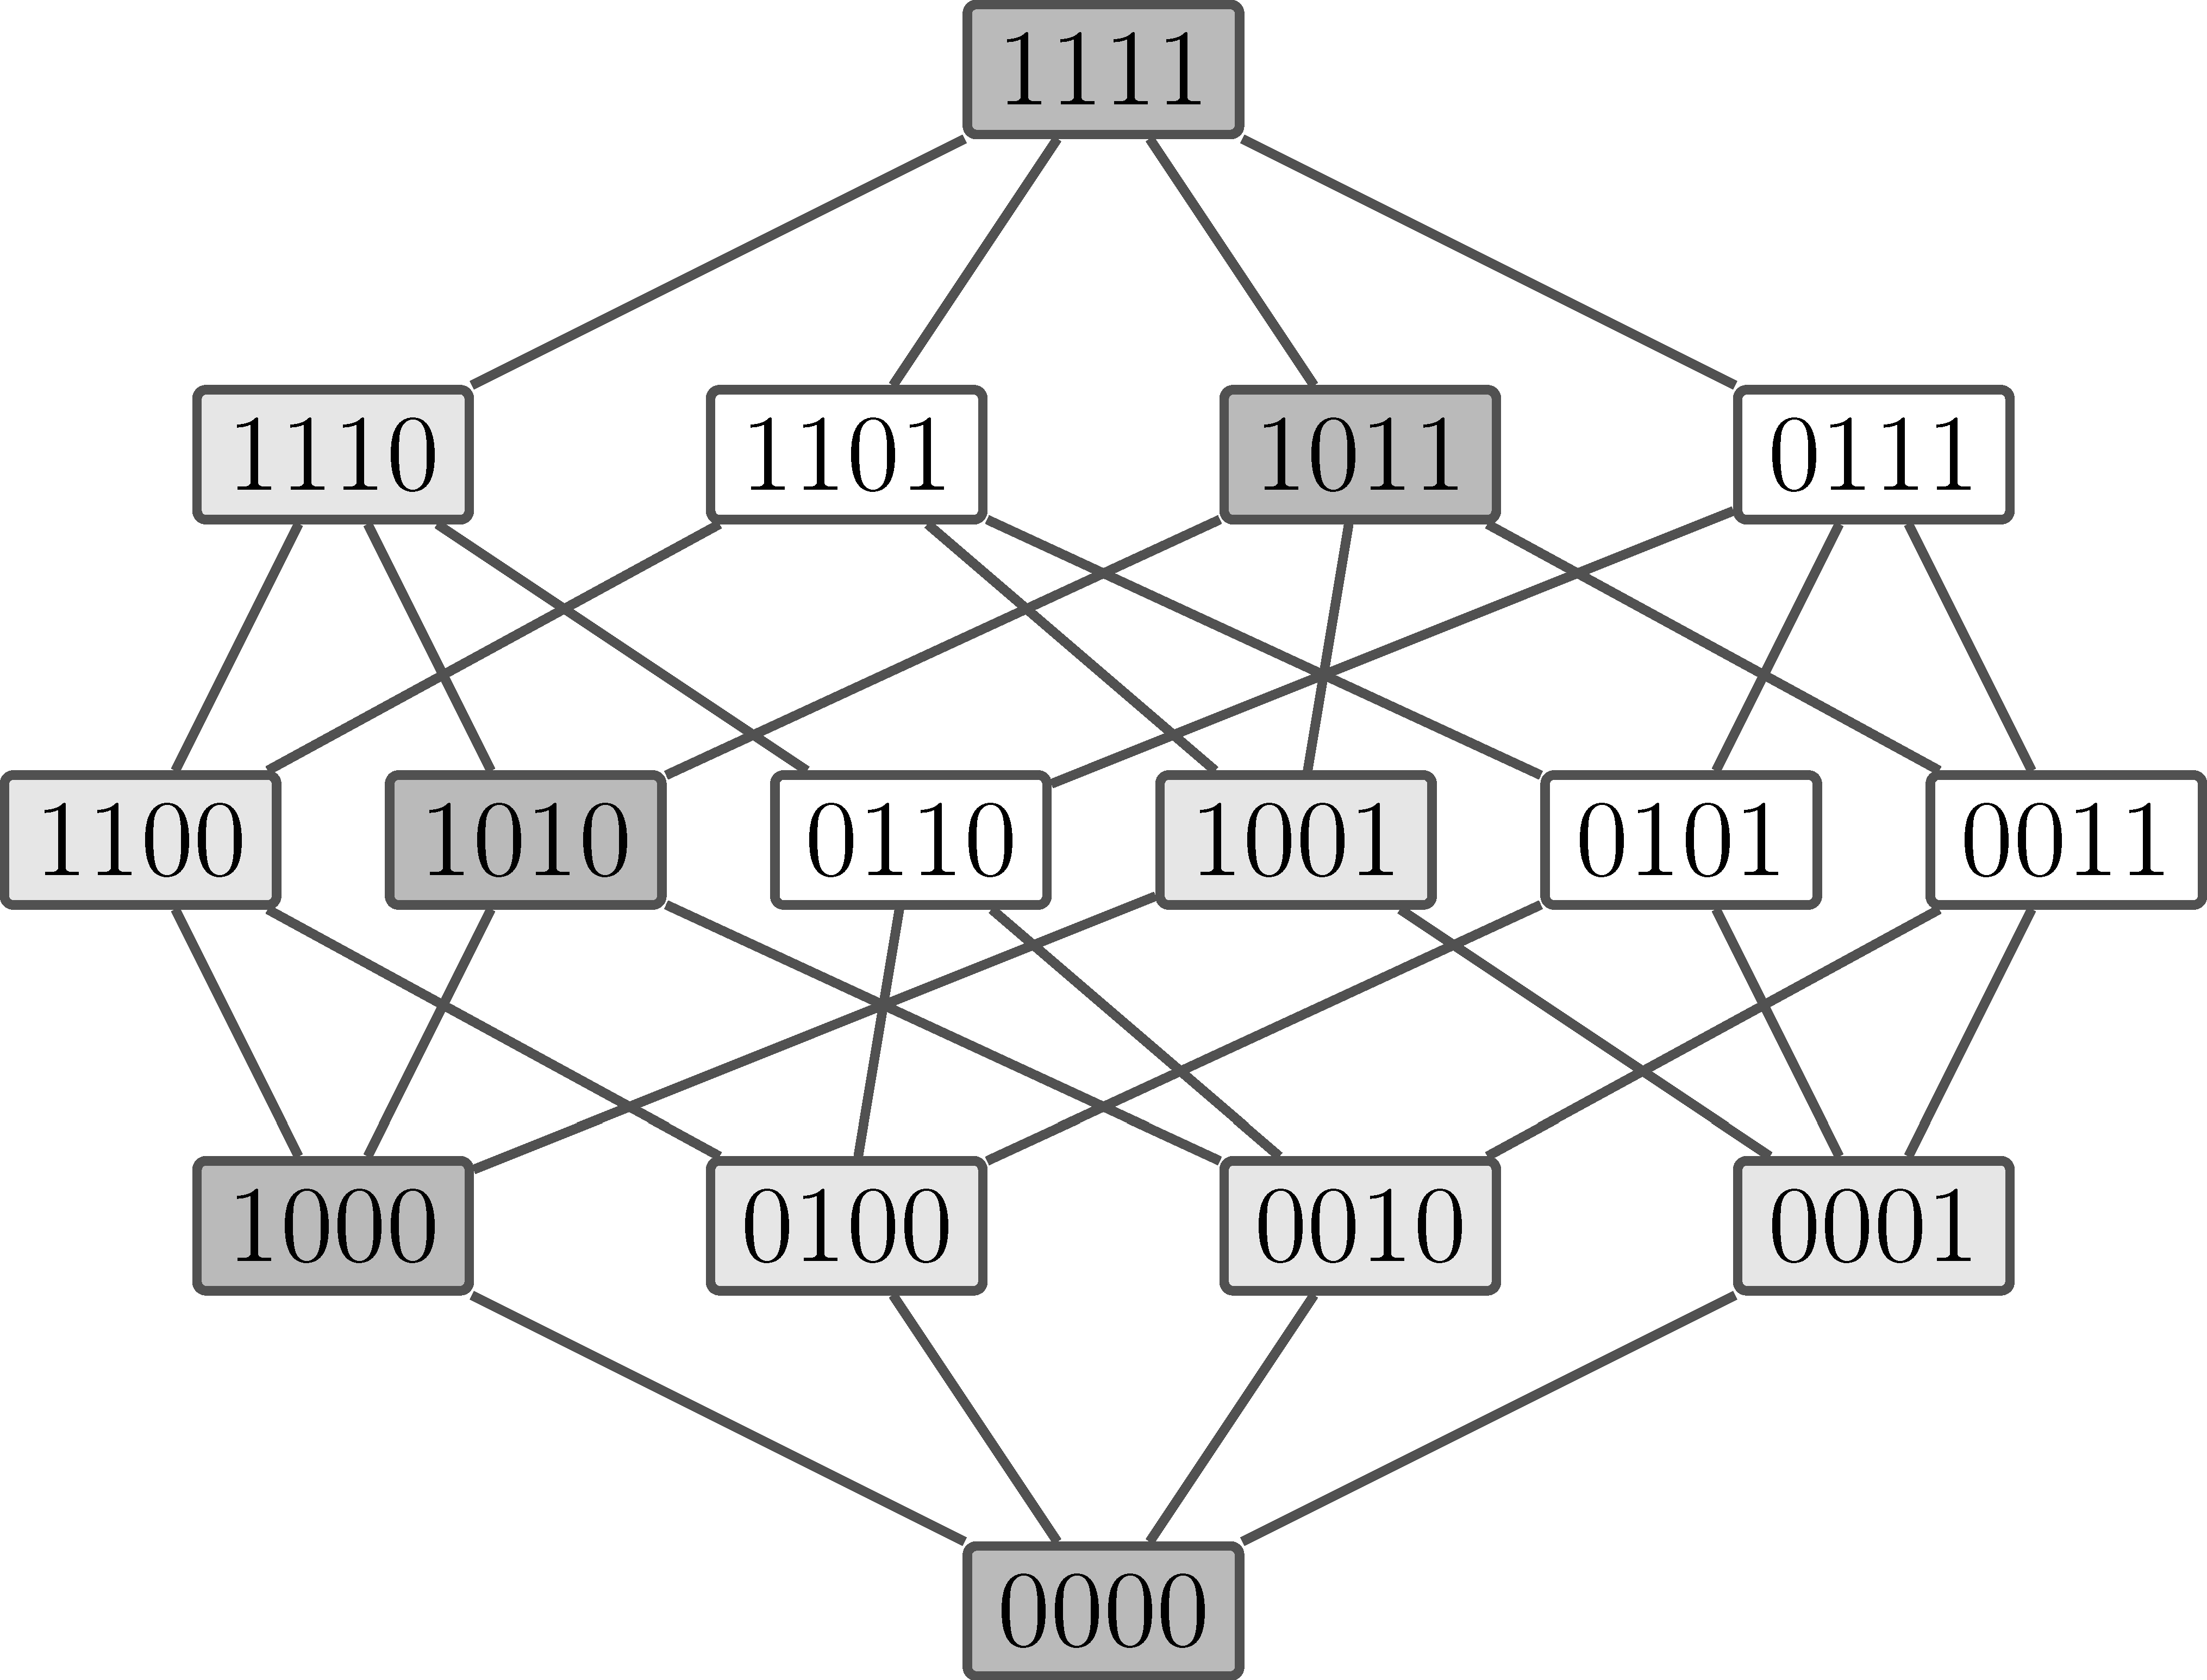
\includegraphics[width=0.8\textwidth,height=\textheight]{chapters/chapter6/Figures/mlr3book_figures-16.png}

}

\caption{\label{fig-sequential-forward-selection}A binary representation
of sequential forward selection with four features. Gray indicates
feature sets that were evaluated, with dark gray indicating the best
feature set in each iteration; white indicates feature sets that were
not evaluated. We start at the bottom with no selected features (all are
`0'). In the next iteration all features are separately tested (each is
`1' separately) and the best option (darkest in row two) is selected.
This continues for selecting the second, third, and fourth features.}

\end{figure}

Wrapper methods can be used with any learner, but need to train or even
resample the learner potentially many times, leading to a
computationally intensive method. All wrapper methods are implemented
via the package
\href{https://mlr3fselect.mlr-org.com}{\texttt{mlr3fselect}}\index{\texttt{mlr3fselect}}.

\begin{tcolorbox}[enhanced jigsaw, opacitybacktitle=0.6, rightrule=.15mm, opacityback=0, arc=.35mm, breakable, titlerule=0mm, colframe=quarto-callout-tip-color-frame, coltitle=black, bottomrule=.15mm, toprule=.15mm, colback=white, colbacktitle=quarto-callout-tip-color!10!white, bottomtitle=1mm, toptitle=1mm, title=\textcolor{quarto-callout-tip-color}{\faLightbulb}\hspace{0.5em}{Feature Selection and HPO}, leftrule=.75mm, left=2mm]

The wrapper-based feature selection explained above is very similar to
the black box optimization approach in HPO
(Chapter~\ref{sec-optimization}), see also
Figure~\ref{fig-optimization-loop-basic}. The major difference is that
we search for well-performing feature subsets instead of hyperparameter
configurations. This similarity is not only true in terms of underlying
concepts and structure, but also with respect to \texttt{mlr3} classes
and API. The API is in many places nearly identical, we can use the same
terminators, results are logged into an archive in a similar fashion to
tuning, and we can also optimize multiple performance measures to create
Pareto-optimal solutions in a similar way

\end{tcolorbox}

\hypertarget{sec-fs-wrapper-example}{%
\subsection{Simple Forward Selection Example}\label{sec-fs-wrapper-example}}

We start with the simple example from above and do sequential forward
selection with \texttt{tsk("penguins")}, similarly to how the sugar
function
\href{https://mlr3tuning.mlr-org.com/reference/tune.html}{\texttt{tune()}}
shown in Section~\ref{sec-autotuner} works, we can use
\href{https://mlr3fselect.mlr-org.com/reference/fselect.html}{\texttt{fselect()}}\index{\texttt{fselect()}}{\marginnote{\begin{footnotesize}\texttt{fselect()}\end{footnotesize}}}
to directly start the optimization and select features.

\begin{Shaded}
\begin{Highlighting}[]
\FunctionTok{library}\NormalTok{(mlr3fselect)}

\CommentTok{\# subset features to ease visualization}
\NormalTok{tsk\_pen }\OtherTok{=} \FunctionTok{tsk}\NormalTok{(}\StringTok{"penguins"}\NormalTok{)}
\NormalTok{tsk\_pen}\SpecialCharTok{$}\FunctionTok{select}\NormalTok{(}\FunctionTok{c}\NormalTok{(}\StringTok{"bill\_depth"}\NormalTok{, }\StringTok{"bill\_length"}\NormalTok{, }\StringTok{"body\_mass"}\NormalTok{,}
  \StringTok{"flipper\_length"}\NormalTok{))}

\NormalTok{instance }\OtherTok{=} \FunctionTok{fselect}\NormalTok{(}
  \AttributeTok{fselector =} \FunctionTok{fs}\NormalTok{(}\StringTok{"sequential"}\NormalTok{),}
  \AttributeTok{task =}\NormalTok{  tsk\_pen,}
  \AttributeTok{learner =}\NormalTok{ lrn\_rpart,}
  \AttributeTok{resampling =} \FunctionTok{rsmp}\NormalTok{(}\StringTok{"cv"}\NormalTok{, }\AttributeTok{folds =} \DecValTok{3}\NormalTok{),}
  \AttributeTok{measure =} \FunctionTok{msr}\NormalTok{(}\StringTok{"classif.acc"}\NormalTok{)}
\NormalTok{)}
\end{Highlighting}
\end{Shaded}

To show all analyzed feature subsets and the corresponding performance,
we use \texttt{as.data.table(instance\$archive)}. In this example, the
\texttt{batch\_nr} column represents the iteration of the sequential
forward selection\index{sequential forward selection} and we start by
looking at the first iteration.

\begin{Shaded}
\begin{Highlighting}[]
\NormalTok{dt }\OtherTok{=} \FunctionTok{as.data.table}\NormalTok{(instance}\SpecialCharTok{$}\NormalTok{archive)}
\NormalTok{dt[batch\_nr }\SpecialCharTok{==} \DecValTok{1}\NormalTok{, }\DecValTok{1}\SpecialCharTok{:}\DecValTok{5}\NormalTok{]}
\end{Highlighting}
\end{Shaded}

\begin{verbatim}
   bill_depth bill_length body_mass flipper_length classif.acc
1:       TRUE       FALSE     FALSE          FALSE      0.7557
2:      FALSE        TRUE     FALSE          FALSE      0.7353
3:      FALSE       FALSE      TRUE          FALSE      0.7064
4:      FALSE       FALSE     FALSE           TRUE      0.7936
\end{verbatim}

We see that the feature \texttt{flipper\_length} achieved the highest
prediction performance in the first iteration and is thus selected. We
plot the performance over the iterations:

\begin{Shaded}
\begin{Highlighting}[]
\FunctionTok{autoplot}\NormalTok{(instance, }\AttributeTok{type =} \StringTok{"performance"}\NormalTok{)}
\end{Highlighting}
\end{Shaded}

\begin{figure}

{\centering 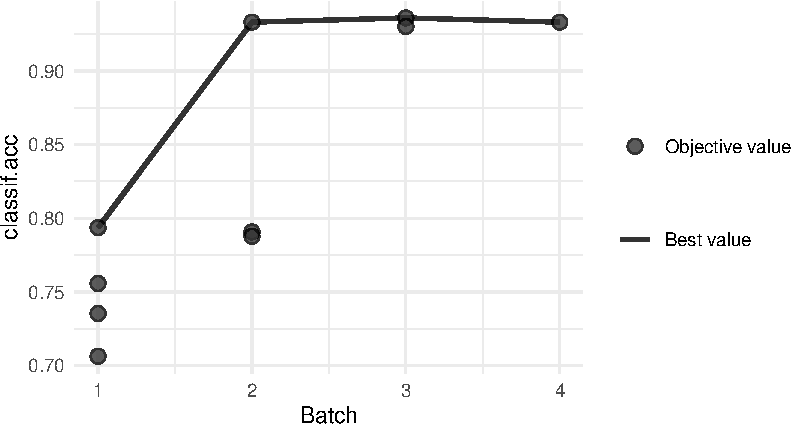
\includegraphics[width=1\textwidth,height=\textheight]{chapters/chapter6/feature_selection_files/figure-pdf/fig-forwardselection-1.pdf}

}

\caption{\label{fig-forwardselection}Model performance in iterations of
sequential forward selection.}

\end{figure}

In the plot, we can see that adding a second feature further improves
the performance to over 90\%. To see which feature was added, we can go
back to the archive and look at the second iteration:

\begin{Shaded}
\begin{Highlighting}[]
\NormalTok{dt[batch\_nr }\SpecialCharTok{==} \DecValTok{2}\NormalTok{, }\DecValTok{1}\SpecialCharTok{:}\DecValTok{5}\NormalTok{]}
\end{Highlighting}
\end{Shaded}

\begin{verbatim}
   bill_depth bill_length body_mass flipper_length classif.acc
1:       TRUE       FALSE     FALSE           TRUE      0.7907
2:      FALSE        TRUE     FALSE           TRUE      0.9331
3:      FALSE       FALSE      TRUE           TRUE      0.7878
\end{verbatim}

The improvement in batch three is small so we may even prefer to select
a marginally worse model with two features to reduce data size.

To directly show the best feature set, we can use
\texttt{\$result\_feature\_set} which returns the features in
alphabetical order (not order selected):

\begin{Shaded}
\begin{Highlighting}[]
\NormalTok{instance}\SpecialCharTok{$}\NormalTok{result\_feature\_set}
\end{Highlighting}
\end{Shaded}

\begin{verbatim}
[1] "bill_depth"     "bill_length"    "flipper_length"
\end{verbatim}

At the heart of \texttt{mlr3fselect} are the R6 classes:

\begin{itemize}
\tightlist
\item
  \texttt{FSelectInstanceSingleCrit},
  \href{https://mlr3fselect.mlr-org.com/reference/FSelectInstanceMultiCrit.html}{\texttt{FSelectInstanceMultiCrit}}:
  These two classes describe the feature selection problem and store the
  results.
\item
  \href{https://mlr3fselect.mlr-org.com/reference/FSelector.html}{\texttt{FSelector}}:
  This class is the base class for implementations of feature selection
  algorithms.
\end{itemize}

Internally, the \texttt{fselect()} function creates an
\href{https://mlr3fselect.mlr-org.com/reference/FSelectInstanceSingleCrit.html}{\texttt{FSelectInstanceSingleCrit}}
object and executes the feature selection with an
\href{https://mlr3fselect.mlr-org.com/reference/FSelector.html}{\texttt{FSelector}}\index{\texttt{FSelector}}
object, based on the selected method, in this example an
\href{https://mlr3fselect.mlr-org.com/reference/mlr_fselectors_sequential.html}{\texttt{FSelectorSequential}}
object. This is similar to what happens in the \texttt{tune()} function
and will be explained in more detail in the following section. It uses
the supplied resampling and measure to evaluate all feature subsets
provided by the \texttt{FSelector} on the task.

In the following two sections, these classes will be created manually,
to learn more about the \texttt{mlr3fselect} package.

\hypertarget{the-fselectinstance-classes}{%
\subsection{The FSelectInstance Classes}\label{the-fselectinstance-classes}}

To create an \texttt{FSelectInstanceSingleCrit} object, we use the sugar
function
\href{https://mlr3fselect.mlr-org.com/reference/fsi.html}{\texttt{fsi()}}\index{\texttt{fsi()}}{\marginnote{\begin{footnotesize}\texttt{fsi()}\end{footnotesize}}}:

\begin{Shaded}
\begin{Highlighting}[]
\NormalTok{instance }\OtherTok{=} \FunctionTok{fsi}\NormalTok{(}
  \AttributeTok{task =}\NormalTok{ tsk\_pen,}
  \AttributeTok{learner =}\NormalTok{ lrn\_rpart,}
  \AttributeTok{resampling =} \FunctionTok{rsmp}\NormalTok{(}\StringTok{"cv"}\NormalTok{, }\AttributeTok{folds =} \DecValTok{3}\NormalTok{),}
  \AttributeTok{measure =} \FunctionTok{msr}\NormalTok{(}\StringTok{"classif.acc"}\NormalTok{),}
  \AttributeTok{terminator =} \FunctionTok{trm}\NormalTok{(}\StringTok{"evals"}\NormalTok{, }\AttributeTok{n\_evals =} \DecValTok{20}\NormalTok{)}
\NormalTok{)}
\end{Highlighting}
\end{Shaded}

Note that we have not selected a feature selection algorithm and thus
did not select any features, yet. We have also supplied a
\texttt{Terminator}, which is used to stop the feature selection, these
are the same objects as we saw in Section~\ref{sec-terminator}.

To start the feature selection, we still need to select an algorithm
which are defined via the
\href{https://mlr3fselect.mlr-org.com/reference/FSelector.html}{\texttt{FSelector}}
class, described in the next section.

\hypertarget{the-fselector-class}{%
\subsection{The FSelector Class}\label{the-fselector-class}}

The \texttt{FSelector}\index{\texttt{FSelector}} class is the base class
for different feature selection algorithms. The following algorithms are
currently implemented in \texttt{mlr3fselect}:

\begin{itemize}
\tightlist
\item
  Random search, trying random feature subsets until termination
  (\texttt{fs("random\_search")})
\item
  Exhaustive search, trying all possible feature subsets
  (\texttt{fs("exhaustive\_search")})
\item
  Sequential search, i.e.~sequential forward or backward selection
  (\texttt{fs("sequential")})
\item
  Recursive feature elimination, which uses a learner's importance
  scores to iteratively remove features with low feature importance
  (\texttt{fs("rfe")})
\item
  Design points, trying all user-supplied feature sets
  (\texttt{fs("design\_points")})
\item
  Genetic search, implementing a genetic algorithm which treats the
  features as a binary sequence and tries to find the best subset with
  mutations (\texttt{fs("genetic\_search")})
\item
  Shadow variable search, which adds permuted copies of all features
  (shadow variables), performs forward selection, and stops when a
  shadow variable is selected (\texttt{fs("shadow\_variable\_search")})
\end{itemize}

Note that all these methods can be stopped (early) with a terminator,
e.g.~an exhaustive search can be stopped after a given number of
evaluations. In this example, we will use a simple random search and
retrieve it from the
\href{https://mlr3fselect.mlr-org.com/reference/mlr_fselectors.html}{\texttt{mlr\_fselectors}}\index{\texttt{mlr\_fselectors}}
dictionary with
\href{https://mlr3fselect.mlr-org.com/reference/fs.html}{\texttt{fs()}}\index{\texttt{fs()}}{\marginnote{\begin{footnotesize}\texttt{fs()}\end{footnotesize}}}.

\begin{Shaded}
\begin{Highlighting}[]
\NormalTok{fselector }\OtherTok{=} \FunctionTok{fs}\NormalTok{(}\StringTok{"random\_search"}\NormalTok{)}
\end{Highlighting}
\end{Shaded}

\hypertarget{starting-the-feature-selection}{%
\subsection{Starting the Feature Selection}\label{starting-the-feature-selection}}

To start the feature selection, we pass the
\texttt{FSelectInstanceSingleCrit} object to the \texttt{\$optimize()}
method of the initialized \texttt{FSelector} object:

\begin{Shaded}
\begin{Highlighting}[]
\NormalTok{fselector}\SpecialCharTok{$}\FunctionTok{optimize}\NormalTok{(instance)}
\end{Highlighting}
\end{Shaded}

The algorithm proceeds as follows

\begin{enumerate}
\def\labelenumi{\arabic{enumi}.}
\tightlist
\item
  The \texttt{FSelector} proposes at least one feature subset or may
  propose multiple subsets to be evaluated in parallel, which can be
  controlled via the setting \texttt{batch\_size}.
\item
  For each feature subset, the given learner is fitted on the task using
  the provided resampling and evaluated with the given measure.
\item
  All evaluations are stored in the archive of the
  \texttt{FSelectInstanceSingleCrit} object.
\item
  The terminator is queried. If the termination criteria are not
  triggered, go to 1).
\item
  Determine the feature subset with the best-observed performance.
\item
  Store the best feature subset as the result in the instance object.
\end{enumerate}

The best feature subset and the corresponding measured performance can
be accessed from the instance:

\begin{Shaded}
\begin{Highlighting}[]
  \FunctionTok{as.data.table}\NormalTok{(instance}\SpecialCharTok{$}\NormalTok{result)[, .(features, classif.acc)]}
\end{Highlighting}
\end{Shaded}

\begin{verbatim}
                               features classif.acc
1: bill_length,body_mass,flipper_length       0.936
\end{verbatim}

As in the forward selection example above, one can investigate all
subset evaluations, which are stored in the archive of the
\texttt{FSelectInstanceSingleCrit} object and can be accessed by using
\texttt{as.data.table()}:

\begin{Shaded}
\begin{Highlighting}[]
\FunctionTok{as.data.table}\NormalTok{(instance}\SpecialCharTok{$}\NormalTok{archive)[}\DecValTok{1}\SpecialCharTok{:}\DecValTok{5}\NormalTok{,}
\NormalTok{  .(bill\_depth, bill\_length, body\_mass, flipper\_length, classif.acc)]}
\end{Highlighting}
\end{Shaded}

\begin{verbatim}
   bill_depth bill_length body_mass flipper_length classif.acc
1:      FALSE        TRUE     FALSE          FALSE      0.7558
2:      FALSE        TRUE     FALSE          FALSE      0.7558
3:      FALSE       FALSE      TRUE          FALSE      0.7210
4:      FALSE        TRUE      TRUE           TRUE      0.9360
5:      FALSE        TRUE      TRUE           TRUE      0.9360
\end{verbatim}

Now the optimized feature subset can be used to subset the task and fit
the model on all observations:

\begin{Shaded}
\begin{Highlighting}[]
\NormalTok{tsk\_pen }\OtherTok{=} \FunctionTok{tsk}\NormalTok{(}\StringTok{"penguins"}\NormalTok{)}

\NormalTok{tsk\_pen}\SpecialCharTok{$}\FunctionTok{select}\NormalTok{(instance}\SpecialCharTok{$}\NormalTok{result\_feature\_set)}
\NormalTok{lrn\_rpart}\SpecialCharTok{$}\FunctionTok{train}\NormalTok{(tsk\_pen)}
\end{Highlighting}
\end{Shaded}

The trained model can now be used to make a prediction on external data.

\hypertarget{sec-multicrit-featsel}{%
\subsection{Optimizing Multiple Performance Measures}\label{sec-multicrit-featsel}}

You might want to use multiple criteria to evaluate the performance of
the feature subsets. With \texttt{mlr3fselect}, the result is the
collection of all feature subsets which are not
Pareto-dominated\index{Pareto optimality} by another subset. Again, we
point out the similarity with HPO and refer to multi-objective
hyperparameter optimization (see Section~\ref{sec-multi-metrics-tuning}
and Karl et al. (2022)).

In the following example, we will perform feature selection on the sonar
dataset. This time, we will use
\href{https://mlr3fselect.mlr-org.com/reference/FSelectInstanceMultiCrit.html}{\texttt{FSelectInstanceMultiCrit}}
to select a subset of features that has high sensitivity, i.e.~TPR, and
high specificity, i.e.~TNR. The feature selection process with multiple
criteria is similar to that with a single criterion, except that we
select two measures to be optimized:

\begin{Shaded}
\begin{Highlighting}[]
\NormalTok{instance }\OtherTok{=} \FunctionTok{fsi}\NormalTok{(}
  \AttributeTok{task =} \FunctionTok{tsk}\NormalTok{(}\StringTok{"sonar"}\NormalTok{),}
  \AttributeTok{learner =}\NormalTok{ lrn\_rpart,}
  \AttributeTok{resampling =} \FunctionTok{rsmp}\NormalTok{(}\StringTok{"holdout"}\NormalTok{),}
  \AttributeTok{measure =} \FunctionTok{msrs}\NormalTok{(}\FunctionTok{c}\NormalTok{(}\StringTok{"classif.tpr"}\NormalTok{, }\StringTok{"classif.tnr"}\NormalTok{)),}
  \AttributeTok{terminator =} \FunctionTok{trm}\NormalTok{(}\StringTok{"evals"}\NormalTok{, }\AttributeTok{n\_evals =} \DecValTok{20}\NormalTok{)}
\NormalTok{)}
\end{Highlighting}
\end{Shaded}

The function
\href{https://mlr3fselect.mlr-org.com/reference/fsi.html}{\texttt{fsi}}
creates an instance of \texttt{FSelectInstanceMultiCrit} if more than
one measure is selected. We now create an
\href{https://mlr3fselect.mlr-org.com/reference/FSelector.html}{\texttt{FSelector}}
and call the \texttt{\$optimize()} function of the \texttt{FSelector}
with the \texttt{FSelectInstanceMultiCrit} object, to search for the
subset of features with the best TPR and FPR. Note that these two
measures cannot both be optimal at the same time (except for the perfect
classifier) and we expect several Pareto-optimal solutions.

\begin{Shaded}
\begin{Highlighting}[]
\NormalTok{fselector }\OtherTok{=} \FunctionTok{fs}\NormalTok{(}\StringTok{"random\_search"}\NormalTok{)}
\NormalTok{fselector}\SpecialCharTok{$}\FunctionTok{optimize}\NormalTok{(instance)}
\end{Highlighting}
\end{Shaded}

As above, the best feature subsets and the corresponding measured
performance can be accessed from the instance.

\begin{Shaded}
\begin{Highlighting}[]
\FunctionTok{as.data.table}\NormalTok{(instance}\SpecialCharTok{$}\NormalTok{result)[, .(features, classif.tpr, classif.tnr)]}
\end{Highlighting}
\end{Shaded}

\begin{verbatim}
                      features classif.tpr classif.tnr
1: V16,V21,V31,V37,V48,V50,...      0.6410      0.8333
2:   V1,V11,V12,V18,V2,V25,...      0.8205      0.7667
3:  V1,V10,V12,V13,V14,V16,...      0.8718      0.7333
4:  V1,V13,V15,V17,V18,V19,...      0.9231      0.6333
\end{verbatim}

We see different tradeoffs of sensitivity and specificity but no feature
subset is dominated by another, i.e.~has worse sensitivity \emph{and}
specificity than any other subset.

\hypertarget{sec-autofselect}{%
\subsection{Nested Resampling}\label{sec-autofselect}}

As in tuning, the performance estimate of the finally selected feature
subset is usually optimistically biased. To obtain unbiased performance
estimates, nested resampling is required and can be set up analogously
to HPO (see Section~\ref{sec-nested-resampling}). We now show this as an
example on the \texttt{sonar} task. The
\href{https://mlr3fselect.mlr-org.com/reference/AutoFSelector.html}{\texttt{AutoFSelector}}\index{\texttt{AutoFSelector}}
class wraps a learner and augments it with automatic feature selection.
Because the \texttt{AutoFSelector} itself inherits from the
\href{https://mlr3.mlr-org.com/reference/Learner.html}{\texttt{Learner}}
base class, it can be used like any other learner. In the example below,
a logistic regression learner is created. This learner is then wrapped
in a random search feature selector that uses holdout (inner) resampling
for performance evaluation. The sugar function
\href{https://mlr3fselect.mlr-org.com/reference/auto_fselector.html}{\texttt{auto\_fselector}}\index{\texttt{auto\_fselector}}{\marginnote{\begin{footnotesize}\texttt{auto\_fselector}\end{footnotesize}}}
can be used to create an instance of \texttt{AutoFSelector}:

\begin{Shaded}
\begin{Highlighting}[]
\NormalTok{afs }\OtherTok{=} \FunctionTok{auto\_fselector}\NormalTok{(}
  \AttributeTok{fselector =} \FunctionTok{fs}\NormalTok{(}\StringTok{"random\_search"}\NormalTok{),}
  \AttributeTok{learner =} \FunctionTok{lrn}\NormalTok{(}\StringTok{"classif.log\_reg"}\NormalTok{),}
  \AttributeTok{resampling =} \FunctionTok{rsmp}\NormalTok{(}\StringTok{"holdout"}\NormalTok{),}
  \AttributeTok{measure =} \FunctionTok{msr}\NormalTok{(}\StringTok{"classif.acc"}\NormalTok{),}
  \AttributeTok{terminator =} \FunctionTok{trm}\NormalTok{(}\StringTok{"evals"}\NormalTok{, }\AttributeTok{n\_evals =} \DecValTok{10}\NormalTok{)}
\NormalTok{)}
\NormalTok{afs}
\end{Highlighting}
\end{Shaded}

\begin{verbatim}
<AutoFSelector:classif.log_reg.fselector>
* Model: list
* Packages: mlr3, mlr3fselect, mlr3learners, stats
* Predict Type: response
* Feature Types: logical, integer, numeric, character, factor,
  ordered
* Properties: loglik, twoclass
\end{verbatim}

The \texttt{AutoFSelector} can then be passed to \texttt{benchmark()} or
\texttt{resample()} for nested resampling
(Section~\ref{sec-nested-resampling}). Below we compare our wrapped
learner \texttt{afs} with a normal logistic regression
\texttt{lrn("classif.log\_reg")}.

\begin{Shaded}
\begin{Highlighting}[]
\NormalTok{grid }\OtherTok{=} \FunctionTok{benchmark\_grid}\NormalTok{(}\FunctionTok{tsk}\NormalTok{(}\StringTok{"sonar"}\NormalTok{), }\FunctionTok{list}\NormalTok{(afs, }\FunctionTok{lrn}\NormalTok{(}\StringTok{"classif.log\_reg"}\NormalTok{)),}
  \FunctionTok{rsmp}\NormalTok{(}\StringTok{"cv"}\NormalTok{, }\AttributeTok{folds =} \DecValTok{3}\NormalTok{))}

\NormalTok{bmr }\OtherTok{=} \FunctionTok{benchmark}\NormalTok{(grid)}\SpecialCharTok{$}\FunctionTok{aggregate}\NormalTok{(}\FunctionTok{msr}\NormalTok{(}\StringTok{"classif.acc"}\NormalTok{))}
\FunctionTok{as.data.table}\NormalTok{(bmr)[, .(learner\_id, classif.acc)]}
\end{Highlighting}
\end{Shaded}

\begin{verbatim}
                  learner_id classif.acc
1: classif.log_reg.fselector      0.7061
2:           classif.log_reg      0.6776
\end{verbatim}

We can see that, in this example, the feature selection improves
prediction performance.

\hypertarget{conclusion-4}{%
\section{Conclusion}\label{conclusion-4}}

In this chapter, we learned how to perform feature selection with
\texttt{mlr3}. We introduced filter and wrapper methods and covered the
optimization of multiple performance measures. Once you have learned
about pipelines we will return to feature selection in
Section~\ref{sec-pipelines-featsel}.

If you are interested in learning more about feature selection then we
recommend an overview of methods in Chandrashekar and Sahin (2014); a
more formal and detailed introduction to filters and wrappers is in
Guyon and Elisseeff (2003), and a benchmark of filter methods was
performed by Bommert et al. (2020).

\hypertarget{tbl-api-feature-selection}{}
\begin{longtable}[]{@{}
  >{\raggedright\arraybackslash}p{(\columnwidth - 4\tabcolsep) * \real{0.3333}}
  >{\raggedright\arraybackslash}p{(\columnwidth - 4\tabcolsep) * \real{0.3333}}
  >{\raggedright\arraybackslash}p{(\columnwidth - 4\tabcolsep) * \real{0.3333}}@{}}
\caption{\label{tbl-api-feature-selection}Important classes and
functions covered in this chapter with underlying class (if applicable),
class constructor or function, and important class fields and methods
(if applicable).}\tabularnewline
\toprule\noalign{}
\begin{minipage}[b]{\linewidth}\raggedright
Class
\end{minipage} & \begin{minipage}[b]{\linewidth}\raggedright
Constructor/Function
\end{minipage} & \begin{minipage}[b]{\linewidth}\raggedright
Fields/Methods
\end{minipage} \\
\midrule\noalign{}
\endfirsthead
\toprule\noalign{}
\begin{minipage}[b]{\linewidth}\raggedright
Class
\end{minipage} & \begin{minipage}[b]{\linewidth}\raggedright
Constructor/Function
\end{minipage} & \begin{minipage}[b]{\linewidth}\raggedright
Fields/Methods
\end{minipage} \\
\midrule\noalign{}
\endhead
\bottomrule\noalign{}
\endlastfoot
\href{https://www.rdocumentation.org/packages/base/topics/funprog}{\texttt{Filter}}
&
\href{https://mlr3filters.mlr-org.com/reference/flt.html}{\texttt{flt()}}
& \texttt{\$calculate()} \\
\href{https://mlr3fselect.mlr-org.com/reference/FSelectInstanceSingleCrit.html}{\texttt{FSelectInstanceSingleCrit}}
or
\href{https://mlr3fselect.mlr-org.com/reference/FSelectInstanceMultiCrit.html}{\texttt{FSelectInstanceMultiCrit}}
&
\href{https://mlr3fselect.mlr-org.com/reference/fselect.html}{\texttt{fselect()}}
& - \\
\href{https://mlr3fselect.mlr-org.com/reference/FSelector.html}{\texttt{FSelector}}
&
\href{https://mlr3fselect.mlr-org.com/reference/fs.html}{\texttt{fs()}}
& \texttt{\$optimize()} \\
\href{https://mlr3fselect.mlr-org.com/reference/AutoFSelector.html}{\texttt{AutoFSelector}}
&
\href{https://mlr3fselect.mlr-org.com/reference/auto_fselector.html}{\texttt{auto\_fselector()}}
& \texttt{\$train()}; \texttt{\$predict()} \\
\end{longtable}

\hypertarget{exercises-4}{%
\section{Exercises}\label{exercises-4}}

\begin{enumerate}
\def\labelenumi{\arabic{enumi}.}
\tightlist
\item
  Compute the correlation filter scores on \texttt{tsk("mtcars")} and
  use the filter to select the five features most strongly correlated
  with the target. Resample \texttt{lrn("regr.kknn")} on both the full
  dataset and the reduced one, and compare both performances based on
  10-fold CV with respect to MSE. NB: Here, we have performed the
  feature filtering outside of CV, which is generally not a good idea as
  it biases the CV performance estimation. To do this properly,
  filtering should be embedded inside the CV via pipelines -- try to
  come back to this exercise after you read
  Chapter~\ref{sec-pipelines-nonseq} to implement this with less bias.
\item
  Apply backward selection to \texttt{tsk("penguins")} with
  \texttt{lrn("classif.rpart")} and holdout resampling by the
  classification accuracy measure. Compare the results with those in
  Section~\ref{sec-fs-wrapper-example} by also running the forward
  selection from that section. Do the selected features differ? Which
  feature selection method reports a higher classification accuracy in
  its \texttt{\$result}?
\item
  There is a problem in the performance comparison in Exercise 2 as
  feature selection is performed on the test-set. Change the process by
  applying forward feature selection with \texttt{auto\_fselector()}.
  Compare the performance to backward feature selection from Exercise 2
  using nested resampling.
\item
  (*) Write a feature selection algorithm that is a hybrid of a filter
  and a wrapper method. This search algorithm should compute filter
  scores for all features and then perform a forward search. But instead
  of tentatively adding all remaining features to the current feature
  set, it should only stochastically try a subset of the available
  features. Features with high filter scores should be added with higher
  probability. Start by coding a stand-alone R method for this search
  (based on a learner, task, resampling, performance measure and some
  control settings). Then, as a stretch goal, see if you can implement
  this as an R6 class inheriting from \texttt{FSelector}.
\end{enumerate}


\part{Pipelines and Preprocessing}

\hypertarget{sec-pipelines}{%
\chapter{Sequential Pipelines}\label{sec-pipelines}}

\vspace{-15mm}\addtocontents{toc}{\textit{Martin Binder and Florian Pfisterer}}

\textbf{Martin Binder} \newline  \emph{Ludwig-Maximilians-Universität
München, and Munich Center for Machine Learning (MCML)}

\textbf{Florian Pfisterer} \newline 
\emph{Ludwig-Maximilians-Universität München} \newline \newline 

\href{https://mlr3.mlr-org.com}{\texttt{mlr3}}\index{\texttt{mlr3}} aims
to provide a layer of abstraction for ML practitioners, allowing users
to quickly swap one algorithm for another without needing expert
knowledge of the underlying implementation. A unified interface for
\href{https://mlr3.mlr-org.com/reference/Task.html}{\texttt{Task}},
\href{https://mlr3.mlr-org.com/reference/Learner.html}{\texttt{Learner}},
and
\href{https://mlr3.mlr-org.com/reference/Measure.html}{\texttt{Measure}}
objects means that complex benchmark and tuning experiments can be run
in just a few lines of code for any off-the-shelf model, i.e., if you
just want to run an experiment using the basic implementation from the
underlying algorithm, we hope we have made this easy for you to do.

\href{https://mlr3pipelines.mlr-org.com}{\texttt{mlr3pipelines}}\index{\texttt{mlr3pipelines}}
(Binder et al. 2021) takes this modularity one step further, extending
it to workflows that may also include data
preprocessing\index{preprocessing} (Chapter~\ref{sec-preprocessing}),
building ensemble\index{ensemble}-models, or even more complicated
meta-models. \texttt{mlr3pipelines} makes it possible to build
individual steps within a \texttt{Learner} out of building blocks, which
inherit from the
\href{https://mlr3pipelines.mlr-org.com/reference/PipeOp.html}{\texttt{PipeOp}}\index{\texttt{PipeOp}}
class. \texttt{PipeOp}s can be connected using directed edges to form a
\href{https://mlr3pipelines.mlr-org.com/reference/Graph.html}{\texttt{Graph}}\index{\texttt{Graph}}
or `pipeline', which represent the flow of data between operations.
During model training, the \texttt{PipeOp}s in a \texttt{Graph}
transform a given \texttt{Task} and subsequent \texttt{PipeOp}s receive
the transformed \texttt{Task} as input. As well as transforming data,
\texttt{PipeOp}s generate a \emph{state}, which is used to inform the
\texttt{PipeOp}s operation during prediction, similar to how learners
learn and store model parameters/weights during training that go on to
inform model prediction. This is visualized in
Figure~\ref{fig-pipelines-state} using the ``Scaling'' \texttt{PipeOp},
which scales features during training and saves the scaling factors as a
state to be used in predictions.

\begin{figure}

{\centering 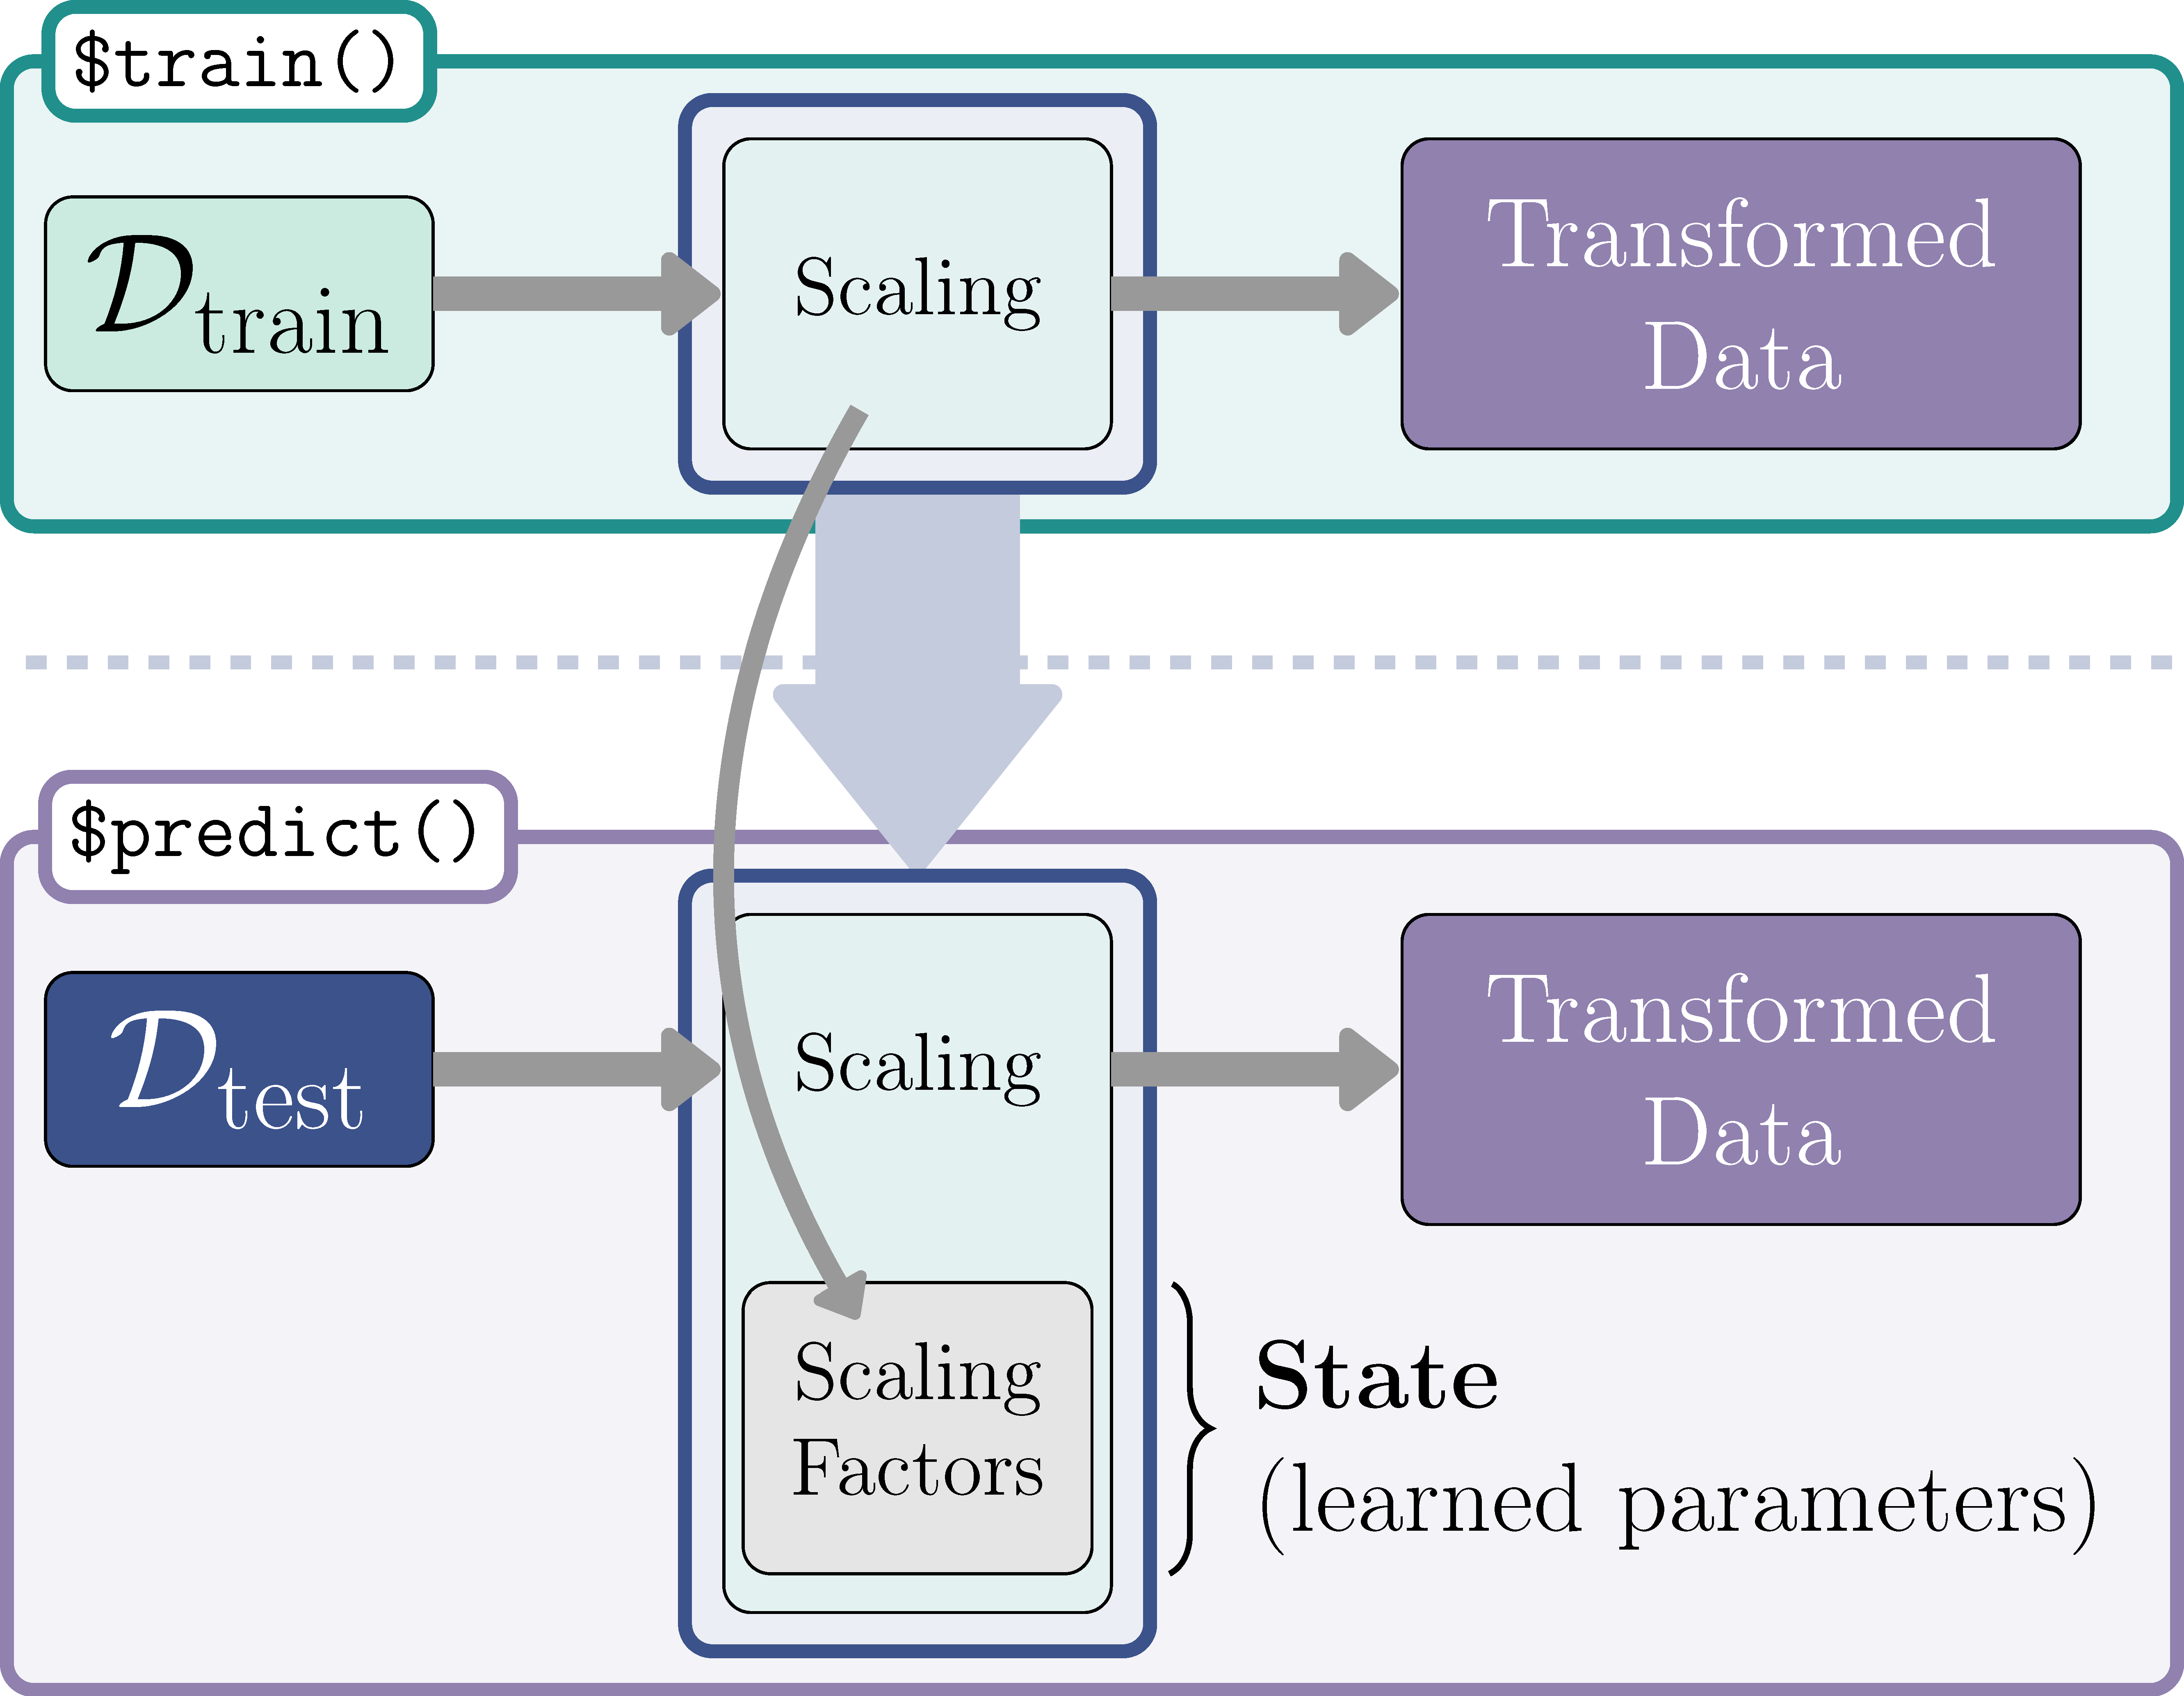
\includegraphics[width=0.7\textwidth,height=\textheight]{chapters/chapter7/Figures/mlr3book_figures-23.png}

}

\caption{\label{fig-pipelines-state}The \texttt{\$train()} method of the
``Scaling'' PipeOp both transforms data (rectangles) as well as creates
a state, which is the scaling factors necessary to transform data during
prediction.}

\end{figure}

We refer to pipelines as either sequential or non-sequential. These
terms should not be confused with ``sequential'' and ``parallel''
processing. In the context of pipelines, ``sequential'' refers to the
movement of data through the pipeline from one \texttt{PipeOp} directly
to the next from start to finish. Sequential pipelines can be visualized
in a straight line -- as we will see in this chapter. In contrast,
non-sequential pipelines see data being processed through
\texttt{PipeOp}s that may have multiple inputs and/or outputs.
Non-sequential pipelines are characterized by multiple branches so data
may be processed by different \texttt{PipeOp}s at different times.
Visually, non-sequential pipelines will not be a straight line from
start to finish, but a more complex graph. In this chapter, we will look
at sequential pipelines and in the next we will focus on non-sequential
pipelines.

\hypertarget{sec-pipelines-pipeops}{%
\section{PipeOp: Pipeline Operators}\label{sec-pipelines-pipeops}}

The basic class of \texttt{mlr3pipelines} is the
\href{https://mlr3pipelines.mlr-org.com/reference/PipeOp.html}{\texttt{PipeOp}}\index{\texttt{PipeOp}}{\marginnote{\begin{footnotesize}\texttt{PipeOp}\end{footnotesize}}},
short for ``pipeline operator''. It represents a transformative
operation on an input (for example, a training
\href{https://mlr3.mlr-org.com/reference/Task.html}{\texttt{Task}}),
resulting in some output. Similarly to a learner, it includes a
\texttt{\$train()} and a \texttt{\$predict()} method. The training phase
typically generates a particular model of the data, which is saved as
the internal
state\index{state}{\marginnote{\begin{footnotesize}State\end{footnotesize}}}.
In the prediction phase, the \texttt{PipeOp} acts on the prediction
\texttt{Task} using information from the saved state. Therefore, just
like a learner, a PipeOp has ``parameters'' (i.e., the state) that are
trained. As well as `parameters', \texttt{PipeOp}s also have
hyperparameters\index{hyperparameters} that can be set by the user when
constructing the \texttt{PipeOp} or by accessing its
\texttt{\$param\_set}. As with other classes, \texttt{PipeOp}s can be
constructed with a sugar function,
\href{https://mlr3pipelines.mlr-org.com/reference/po.html}{\texttt{po()}}\index{\texttt{po()}}{\marginnote{\begin{footnotesize}\texttt{po()}\end{footnotesize}}},
or \texttt{pos()} for multiple \texttt{PipeOp}s, and all available
\texttt{PipeOp}s are made available in the dictionary
\href{https://mlr3pipelines.mlr-org.com/reference/mlr_pipeops.html}{\texttt{mlr\_pipeops}}\index{\texttt{mlr\_pipeops}}{\marginnote{\begin{footnotesize}\texttt{mlr\_pipeops}\end{footnotesize}}}.
An up-to-date list of \texttt{PipeOp}s contained in
\texttt{mlr3pipelines} with links to their documentation can be found at
\url{https://mlr-org.com/pipeops.html}, a small subset of these are
printed below. If you want to extend \texttt{mlr3pipelines} with a
\texttt{PipeOp} that has not been implemented, have a look at our
vignette on extending \texttt{PipeOp}s by running:
\texttt{vignette("extending",\ package\ =\ "mlr3pipelines")}.

\begin{Shaded}
\begin{Highlighting}[]
\FunctionTok{as.data.table}\NormalTok{(}\FunctionTok{po}\NormalTok{())[}\DecValTok{1}\SpecialCharTok{:}\DecValTok{6}\NormalTok{, }\DecValTok{1}\SpecialCharTok{:}\DecValTok{2}\NormalTok{]}
\end{Highlighting}
\end{Shaded}

\begin{verbatim}
              key                                      label
1:         boxcox Box-Cox Transformation of Numeric Features
2:         branch                             Path Branching
3:          chunk          Chunk Input into Multiple Outputs
4: classbalancing                            Class Balancing
5:     classifavg                   Majority Vote Prediction
6:   classweights         Class Weights for Sample Weighting
\end{verbatim}

Let us now take a look at a \texttt{PipeOp} in practice using principal
component analysis\index{principal component analysis}
(PCA)\index{PCA|see{principal component analysis}} as an example, which
is implemented in
\href{https://mlr3pipelines.mlr-org.com/reference/mlr_pipeops_pca.html}{\texttt{PipeOpPCA}}.
Below we construct the \texttt{PipeOp} using its ID \texttt{"pca"} and
inspect it.

\begin{Shaded}
\begin{Highlighting}[]
\FunctionTok{library}\NormalTok{(mlr3pipelines)}

\NormalTok{po\_pca }\OtherTok{=} \FunctionTok{po}\NormalTok{(}\StringTok{"pca"}\NormalTok{, }\AttributeTok{center =} \ConstantTok{TRUE}\NormalTok{)}
\NormalTok{po\_pca}
\end{Highlighting}
\end{Shaded}

\begin{verbatim}
PipeOp: <pca> (not trained)
values: <center=TRUE>
Input channels <name [train type, predict type]>:
  input [Task,Task]
Output channels <name [train type, predict type]>:
  output [Task,Task]
\end{verbatim}

On printing, we can see that the \texttt{PipeOp} has not been trained
and that we have changed some of the hyperparameters from their default
values. The \texttt{Input\ channels} and \texttt{Output\ channels} lines
provide information about the input and output types of this PipeOp. The
PCA \texttt{PipeOp} takes one input (named ``input'') of type
``\texttt{Task}'', both during training and prediction
(``\texttt{input\ {[}Task,Task{]}}''), and produces one called
``output'' that is also of type ``\texttt{Task}'' in both phases
(``\texttt{output\ {[}Task,Task{]}}''). This highlights a key difference
from the \texttt{Learner} class: \texttt{PipeOp}s can return results
after the training phase.

A \texttt{PipeOp} can be trained using \texttt{\$train()}, which can
have multiple inputs and outputs. Both inputs and outputs are passed as
elements in a single \texttt{list}. The \texttt{"pca"} \texttt{PipeOp}
takes as input the original task and after training returns the task
with features replaced by their principal components.

\begin{Shaded}
\begin{Highlighting}[]
\NormalTok{tsk\_small }\OtherTok{=} \FunctionTok{tsk}\NormalTok{(}\StringTok{"penguins\_simple"}\NormalTok{)}\SpecialCharTok{$}\FunctionTok{select}\NormalTok{(}\FunctionTok{c}\NormalTok{(}\StringTok{"bill\_depth"}\NormalTok{, }\StringTok{"bill\_length"}\NormalTok{))}
\NormalTok{poin }\OtherTok{=} \FunctionTok{list}\NormalTok{(tsk\_small}\SpecialCharTok{$}\FunctionTok{clone}\NormalTok{()}\SpecialCharTok{$}\FunctionTok{filter}\NormalTok{(}\DecValTok{1}\SpecialCharTok{:}\DecValTok{5}\NormalTok{))}
\NormalTok{poout }\OtherTok{=}\NormalTok{ po\_pca}\SpecialCharTok{$}\FunctionTok{train}\NormalTok{(poin) }\CommentTok{\# poin: Task in a list}
\NormalTok{poout }\CommentTok{\# list with a single element \textquotesingle{}output\textquotesingle{}}
\end{Highlighting}
\end{Shaded}

\begin{verbatim}
$output
<TaskClassif:penguins> (5 x 3): Simplified Palmer Penguins
* Target: species
* Properties: multiclass
* Features (2):
  - dbl (2): PC1, PC2
\end{verbatim}

\begin{Shaded}
\begin{Highlighting}[]
\NormalTok{poout[[}\DecValTok{1}\NormalTok{]]}\SpecialCharTok{$}\FunctionTok{head}\NormalTok{()}
\end{Highlighting}
\end{Shaded}

\begin{verbatim}
   species     PC1       PC2
1:  Adelie  0.1561  0.005716
2:  Adelie  1.2677  0.789534
3:  Adelie  1.5336 -0.174460
4:  Adelie -2.1096  0.998977
5:  Adelie -0.8478 -1.619768
\end{verbatim}

During training, PCA transforms incoming data by rotating it in such a
way that features become uncorrelated and are ordered by their
contribution to the total variance. The rotation matrix is also saved in
the internal \texttt{\$state} field during training (shown in
Figure~\ref{fig-pipelines-state}), which is then used during predictions
and applied to new data.

\begin{Shaded}
\begin{Highlighting}[]
\NormalTok{po\_pca}\SpecialCharTok{$}\NormalTok{state}
\end{Highlighting}
\end{Shaded}

\begin{verbatim}
Standard deviations (1, .., p=2):
[1] 1.513 1.034

Rotation (n x k) = (2 x 2):
                PC1     PC2
bill_depth  -0.6116 -0.7911
bill_length  0.7911 -0.6116
\end{verbatim}

Once trained, the \texttt{\$predict()} function can then access the
saved state to operate on the test data, which again is passed as a
\texttt{list}:

\begin{Shaded}
\begin{Highlighting}[]
\NormalTok{tsk\_onepenguin }\OtherTok{=}\NormalTok{ tsk\_small}\SpecialCharTok{$}\FunctionTok{clone}\NormalTok{()}\SpecialCharTok{$}\FunctionTok{filter}\NormalTok{(}\DecValTok{42}\NormalTok{)}
\NormalTok{poin }\OtherTok{=} \FunctionTok{list}\NormalTok{(tsk\_onepenguin)}
\NormalTok{poout }\OtherTok{=}\NormalTok{ po\_pca}\SpecialCharTok{$}\FunctionTok{predict}\NormalTok{(poin)}
\NormalTok{poout[[}\DecValTok{1}\NormalTok{]]}\SpecialCharTok{$}\FunctionTok{data}\NormalTok{()}
\end{Highlighting}
\end{Shaded}

\begin{verbatim}
   species   PC1    PC2
1:  Adelie 1.555 -1.455
\end{verbatim}

\hypertarget{sec-pipelines-graphs}{%
\section{Graph: Networks of PipeOps}\label{sec-pipelines-graphs}}

\texttt{PipeOp}s represent individual computational steps in machine
learning pipelines. These pipelines themselves are defined by
\href{https://mlr3pipelines.mlr-org.com/reference/Graph.html}{\texttt{Graph}}\index{\texttt{Graph}}
objects. A \texttt{Graph} is a collection of \texttt{PipeOp}s with
``edges'' that guide the flow of data.

The most convenient way of building a \texttt{Graph} is to connect a
sequence of \texttt{PipeOp}s using the
\texttt{\%\textgreater{}\textgreater{}\%}-operator
{\marginnote{\begin{footnotesize}\texttt{\%\textgreater{}\textgreater{}\%}\end{footnotesize}}}
\index{\%>>\%} (read ``double-arrow'') operator. When given two
\texttt{PipeOp}s, this operator creates a \texttt{Graph} that first
executes the left-hand \texttt{PipeOp}, followed by the right-hand one.
It can also be used to connect a \texttt{Graph} with a \texttt{PipeOp},
or with another \texttt{Graph}. The following example uses
\texttt{po("mutate")} to add a new feature to the task, and
\texttt{po("scale")} to then scale\index{scale} and center all numeric
features.

\begin{Shaded}
\begin{Highlighting}[]
\NormalTok{po\_mutate }\OtherTok{=} \FunctionTok{po}\NormalTok{(}\StringTok{"mutate"}\NormalTok{,}
  \AttributeTok{mutation =} \FunctionTok{list}\NormalTok{(}\AttributeTok{bill\_ratio =} \SpecialCharTok{\textasciitilde{}}\NormalTok{bill\_length }\SpecialCharTok{/}\NormalTok{ bill\_depth)}
\NormalTok{)}
\NormalTok{po\_scale }\OtherTok{=} \FunctionTok{po}\NormalTok{(}\StringTok{"scale"}\NormalTok{)}
\NormalTok{graph }\OtherTok{=}\NormalTok{ po\_mutate }\SpecialCharTok{\%\textgreater{}\textgreater{}\%}\NormalTok{ po\_scale}
\NormalTok{graph}
\end{Highlighting}
\end{Shaded}

\begin{verbatim}
Graph with 2 PipeOps:
     ID         State sccssors prdcssors
 mutate <<UNTRAINED>>    scale          
  scale <<UNTRAINED>>             mutate
\end{verbatim}

The output provides information about the layout of the Graph. For each
\texttt{PipOp} (\texttt{ID}), we can see information about the state
(\texttt{State}), as well as a list of its successors
(\texttt{sccssors}), which are \texttt{PipeOp}s that come directly after
the given \texttt{PipeOp}, and its predecessors (\texttt{prdcssors}),
the \texttt{PipeOp}s that are connected to its input. In this simple
\texttt{Graph}, the output of the \texttt{"mutate"} \texttt{PipeOp} is
passed directly to the \texttt{"scale"} \texttt{PipeOp} and neither
takes any other inputs or outputs from other \texttt{PipeOp}s. The
\texttt{\$plot()}\index{\texttt{Graph}!\texttt{\$plot()}}{\marginnote{\begin{footnotesize}\$plot()\end{footnotesize}}}
method can be used to visualize the graph.

\begin{Shaded}
\begin{Highlighting}[]
\NormalTok{graph}\SpecialCharTok{$}\FunctionTok{plot}\NormalTok{(}\AttributeTok{horizontal =} \ConstantTok{TRUE}\NormalTok{)}
\end{Highlighting}
\end{Shaded}

\begin{figure}

{\centering 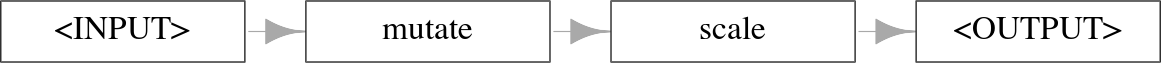
\includegraphics[width=1\textwidth,height=\textheight]{chapters/chapter7/sequential_pipelines_files/figure-pdf/fig-pipelines-basic-plot-1.png}

}

\caption{\label{fig-pipelines-basic-plot}Simple sequential pipeline
plot.}

\end{figure}

The plot demonstrates how a \texttt{Graph} is simply a collection of
\texttt{PipeOp}s that are connected by `edges'. The collection of
\texttt{PipeOp}s inside a \texttt{Graph} can be accessed through the
\texttt{\$pipeops} \index{\$pipeops} field. The \texttt{\$edges}
\index{\$edges} field can be used to access edges, which returns a
\texttt{data.table} listing the ``source'' (\texttt{src\_id},
\texttt{src\_channel}) and ``destination'' (\texttt{dst\_id},
\texttt{dst\_channel}) of data flowing along each edge
{\marginnote{\begin{footnotesize}\texttt{\$edges}/\texttt{\$pipeops}\end{footnotesize}}}.

\begin{Shaded}
\begin{Highlighting}[]
\NormalTok{graph}\SpecialCharTok{$}\NormalTok{pipeops}
\end{Highlighting}
\end{Shaded}

\begin{verbatim}
$mutate
PipeOp: <mutate> (not trained)
values: <mutation=<list>, delete_originals=FALSE>
Input channels <name [train type, predict type]>:
  input [Task,Task]
Output channels <name [train type, predict type]>:
  output [Task,Task]

$scale
PipeOp: <scale> (not trained)
values: <robust=FALSE>
Input channels <name [train type, predict type]>:
  input [Task,Task]
Output channels <name [train type, predict type]>:
  output [Task,Task]
\end{verbatim}

\begin{Shaded}
\begin{Highlighting}[]
\NormalTok{graph}\SpecialCharTok{$}\NormalTok{edges}
\end{Highlighting}
\end{Shaded}

\begin{verbatim}
   src_id src_channel dst_id dst_channel
1: mutate      output  scale       input
\end{verbatim}

Instead of using \texttt{\%\textgreater{}\textgreater{}\%}, you can also
create a \texttt{Graph} explicitly using the \texttt{\$add\_pipeop()}
and \texttt{\$add\_edge()} methods to create \texttt{PipeOp}s and the
edges connecting them:

\begin{Shaded}
\begin{Highlighting}[]
\NormalTok{graph }\OtherTok{=}\NormalTok{ Graph}\SpecialCharTok{$}\FunctionTok{new}\NormalTok{()}\SpecialCharTok{$}
  \FunctionTok{add\_pipeop}\NormalTok{(po\_mutate)}\SpecialCharTok{$}
  \FunctionTok{add\_pipeop}\NormalTok{(po\_scale)}\SpecialCharTok{$}
  \FunctionTok{add\_edge}\NormalTok{(}\StringTok{"mutate"}\NormalTok{, }\StringTok{"scale"}\NormalTok{)}
\end{Highlighting}
\end{Shaded}

\begin{tcolorbox}[enhanced jigsaw, opacitybacktitle=0.6, rightrule=.15mm, opacityback=0, arc=.35mm, breakable, titlerule=0mm, colframe=quarto-callout-tip-color-frame, coltitle=black, bottomrule=.15mm, toprule=.15mm, colback=white, colbacktitle=quarto-callout-tip-color!10!white, bottomtitle=1mm, toptitle=1mm, title=\textcolor{quarto-callout-tip-color}{\faLightbulb}\hspace{0.5em}{Graphs and DAGs}, leftrule=.75mm, left=2mm]

The
\href{https://mlr3pipelines.mlr-org.com/reference/Graph.html}{\texttt{Graph}}
class represents an object similar to a directed acyclic
graph\index{directed acyclic graph}
(DAG)\index{DAG|see{Directed Acyclic Graph}}, since the input of a
\href{https://mlr3pipelines.mlr-org.com/reference/PipeOp.html}{\texttt{PipeOp}}
cannot depend on its output and hence cycles are not allowed. However,
the resemblance to a DAG is not perfect, since the \texttt{Graph} class
allows for multiple edges between nodes. A term such as ``directed
acyclic multigraph'' would be more accurate, but we use ``graph'' for
simplicity.

\end{tcolorbox}

Once built, a \texttt{Graph} can be used by calling \texttt{\$train()}
and \texttt{\$predict()} as if it were a \texttt{Learner} (though it
still outputs a \texttt{list} during training and prediction):

\begin{Shaded}
\begin{Highlighting}[]
\NormalTok{result }\OtherTok{=}\NormalTok{ graph}\SpecialCharTok{$}\FunctionTok{train}\NormalTok{(tsk\_small)}
\NormalTok{result}
\end{Highlighting}
\end{Shaded}

\begin{verbatim}
$scale.output
<TaskClassif:penguins> (333 x 4): Simplified Palmer Penguins
* Target: species
* Properties: multiclass
* Features (3):
  - dbl (3): bill_depth, bill_length, bill_ratio
\end{verbatim}

\begin{Shaded}
\begin{Highlighting}[]
\NormalTok{result[[}\DecValTok{1}\NormalTok{]]}\SpecialCharTok{$}\FunctionTok{data}\NormalTok{()[}\DecValTok{1}\SpecialCharTok{:}\DecValTok{3}\NormalTok{]}
\end{Highlighting}
\end{Shaded}

\begin{verbatim}
   species bill_depth bill_length bill_ratio
1:  Adelie     0.7796     -0.8947    -1.0421
2:  Adelie     0.1194     -0.8216    -0.6804
3:  Adelie     0.4241     -0.6753    -0.7435
\end{verbatim}

\begin{Shaded}
\begin{Highlighting}[]
\NormalTok{result }\OtherTok{=}\NormalTok{ graph}\SpecialCharTok{$}\FunctionTok{predict}\NormalTok{(tsk\_onepenguin)}
\NormalTok{result[[}\DecValTok{1}\NormalTok{]]}\SpecialCharTok{$}\FunctionTok{head}\NormalTok{()}
\end{Highlighting}
\end{Shaded}

\begin{verbatim}
   species bill_depth bill_length bill_ratio
1:  Adelie     0.9319      -0.529    -0.8963
\end{verbatim}

\hypertarget{sec-pipelines-sequential}{%
\section{Sequential Learner-Pipelines}\label{sec-pipelines-sequential}}

Possibly the most common application for \texttt{mlr3pipelines} is to
use it to perform preprocessing\index{preprocessing} tasks, such as
missing value imputation\index{imputation} or factor
encoding\index{factor encoding}, and to then feed the resulting data
into a \texttt{Learner} -- we will see more of this in practice in
Chapter~\ref{sec-preprocessing}. A \texttt{Graph} representing this
workflow manipulates data and fits a \texttt{Learner}-model during
training, ensuring that the data is processed the same way during the
prediction stage. Conceptually, the process may look as shown in
Figure~\ref{fig-pipelines-pipeline}.

\begin{figure}

{\centering 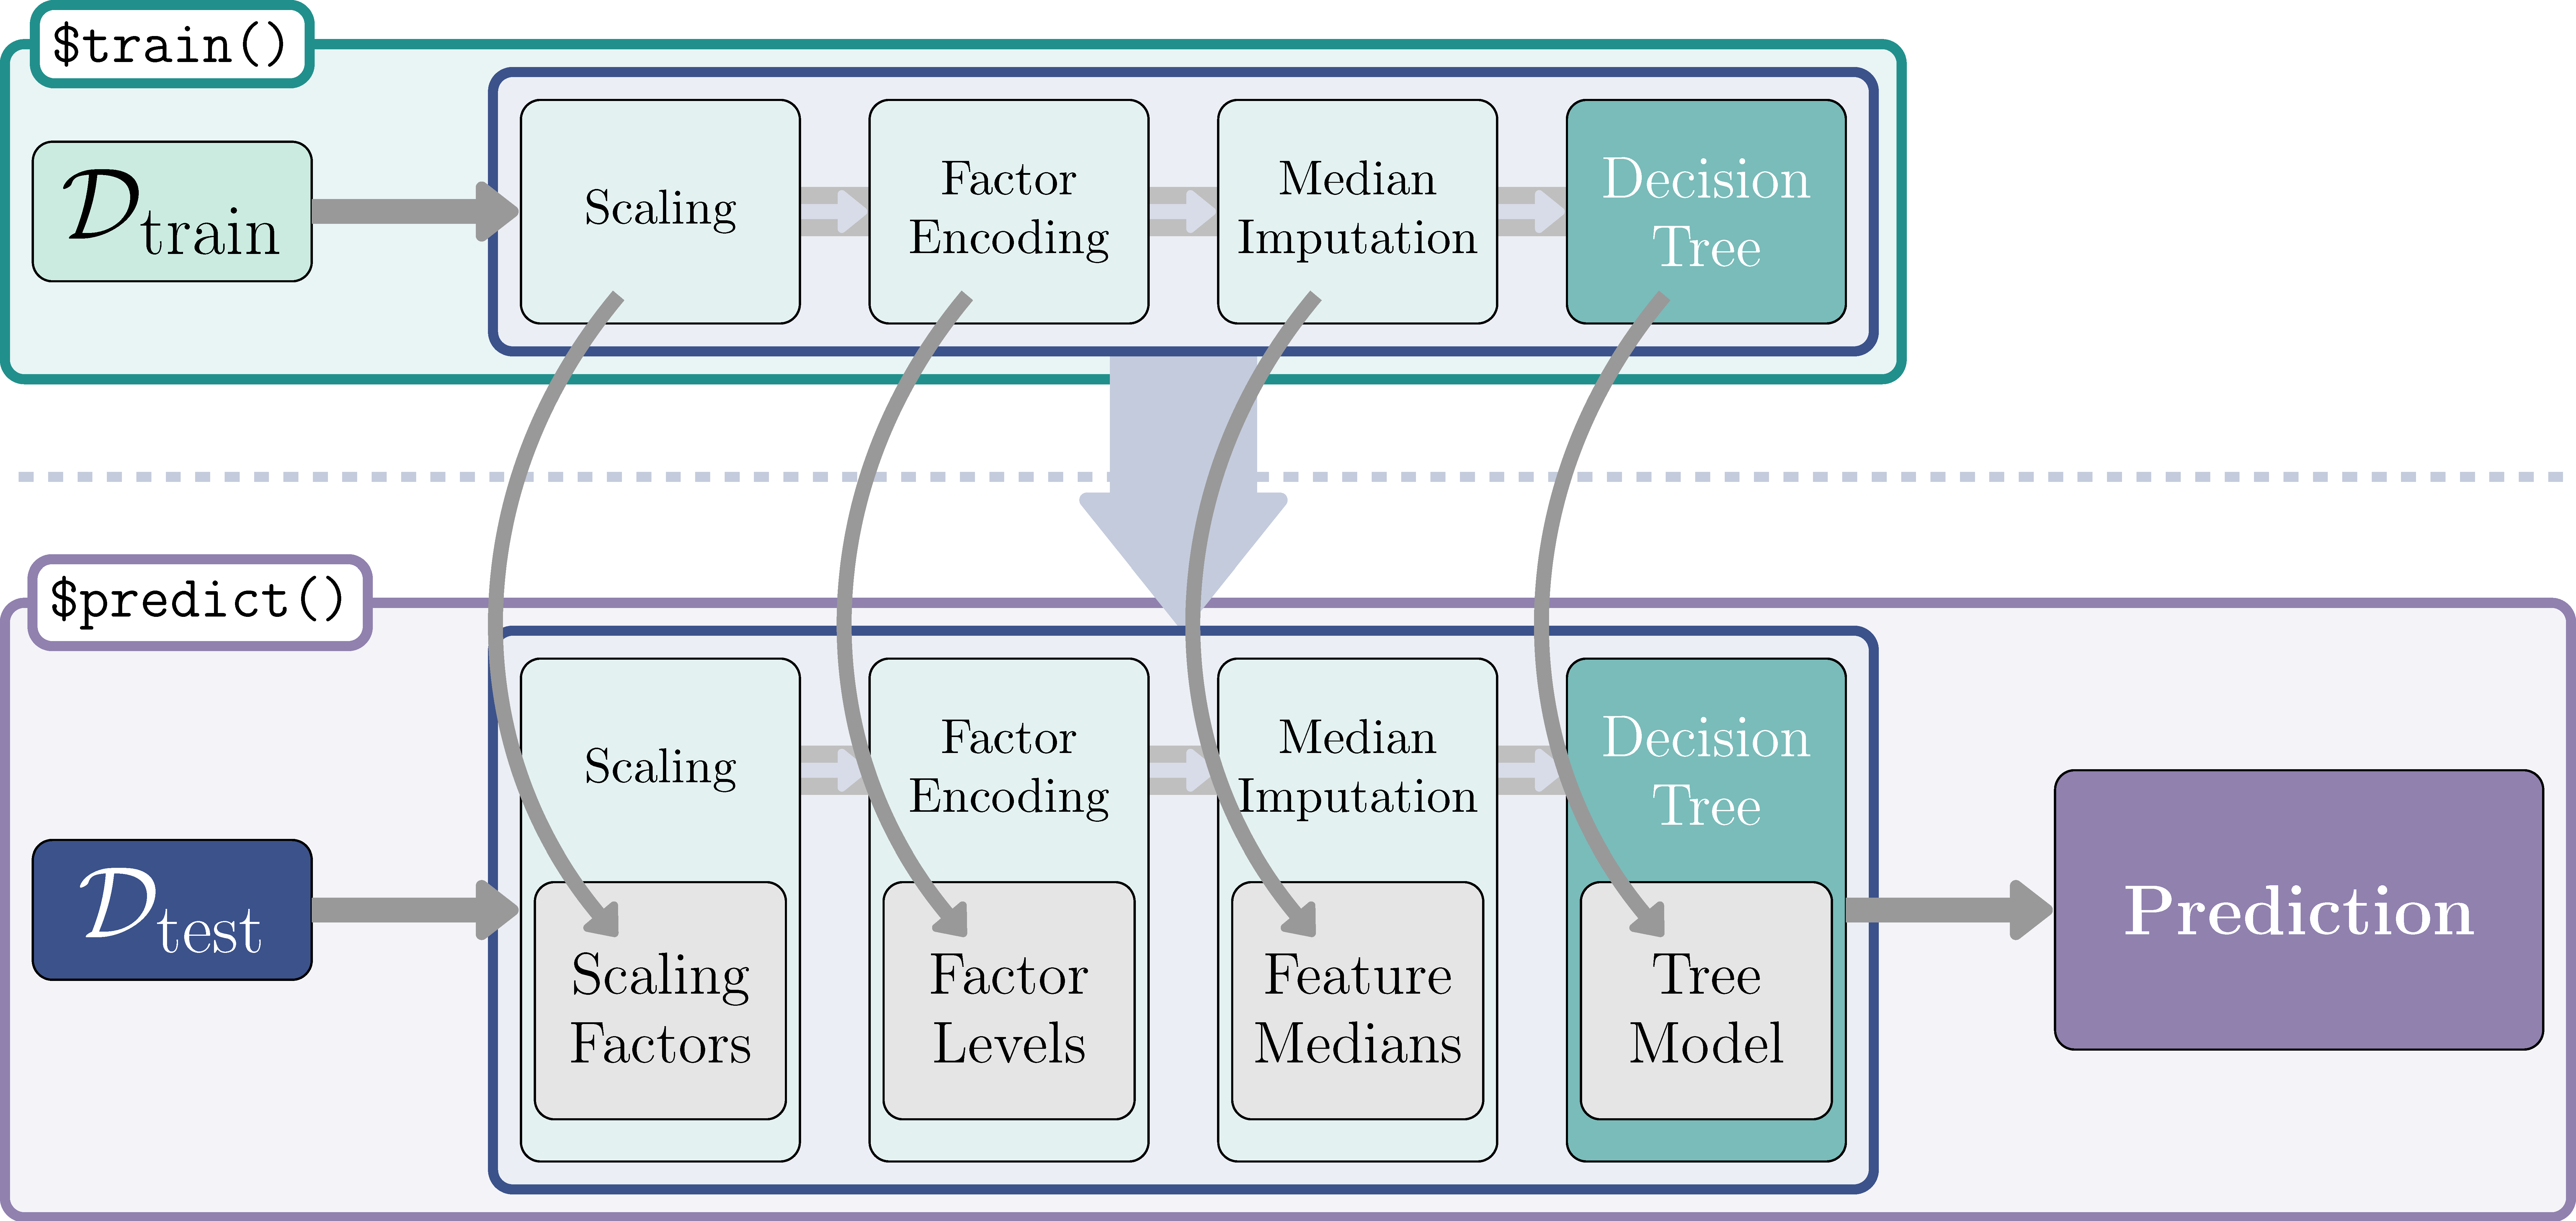
\includegraphics[width=1\textwidth,height=\textheight]{chapters/chapter7/Figures/mlr3book_figures-22.png}

}

\caption{\label{fig-pipelines-pipeline}Conceptualization of training and
prediction process inside a sequential learner-pipeline. During training
(top row), the data is passed along the preprocessing operators, each of
which modifies the data and creates a \texttt{\$state}. Finally, the
learner receives the data and a model is created. During prediction
(bottom row), data is likewise transformed by preprocessing operators,
using their respective \texttt{\$state} (gray boxes) information in the
process. The learner then receives data that has the same format as the
data seen during training, and makes a prediction.}

\end{figure}

\hypertarget{learners-as-pipeops-and-graphs-as-learners}{%
\subsection{Learners as PipeOps and Graphs as
Learners}\label{learners-as-pipeops-and-graphs-as-learners}}

In Figure~\ref{fig-pipelines-pipeline} the final \texttt{PipeOp} is a
\texttt{Learner}. \texttt{Learner} objects can be converted to
\texttt{PipeOp}s with
\href{https://mlr3pipelines.mlr-org.com/reference/as_pipeop.html}{\texttt{as\_pipeop()}},
however, this is only necessary if you choose to manually create a graph
instead of using \texttt{\%\textgreater{}\textgreater{}\%}. With either
method, internally \texttt{Learner}s are passed to
\texttt{po("learner")}. The following code creates a
\href{https://mlr3pipelines.mlr-org.com/reference/Graph.html}{\texttt{Graph}}
that uses \texttt{po("imputesample")} to impute\index{imputation}
missing values by sampling from observed values
(Section~\ref{sec-preprocessing-missing}) then fits a logistic
regression\index{logistic regression} on the transformed task.

\begin{Shaded}
\begin{Highlighting}[]
\NormalTok{lrn\_logreg }\OtherTok{=} \FunctionTok{lrn}\NormalTok{(}\StringTok{"classif.log\_reg"}\NormalTok{)}
\NormalTok{graph }\OtherTok{=} \FunctionTok{po}\NormalTok{(}\StringTok{"imputesample"}\NormalTok{) }\SpecialCharTok{\%\textgreater{}\textgreater{}\%}\NormalTok{ lrn\_logreg}
\NormalTok{graph}\SpecialCharTok{$}\FunctionTok{plot}\NormalTok{(}\AttributeTok{horizontal =} \ConstantTok{TRUE}\NormalTok{)}
\end{Highlighting}
\end{Shaded}

\begin{figure}

{\centering 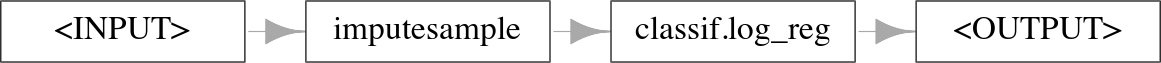
\includegraphics[width=1\textwidth,height=\textheight]{chapters/chapter7/sequential_pipelines_files/figure-pdf/fig-pipelines-learnerpipeop-1.png}

}

\caption{\label{fig-pipelines-learnerpipeop}\texttt{"imputesample"} and
\texttt{"learner"} PipeOps in a sequential pipeline.}

\end{figure}

We have seen how training and predicting \texttt{Graph}s is possible but
has a slightly different design to \texttt{Learner} objects, i.e.,
inputs and outputs during both training and predicting are \texttt{list}
objects. To use a \texttt{Graph} as a \texttt{Learner} with an identical
interface, it can be wrapped in a
\href{https://mlr3pipelines.mlr-org.com/reference/mlr_learners_graph.html}{\texttt{GraphLearner}}\index{\texttt{GraphLearner}}
object with
\href{https://mlr3.mlr-org.com/reference/as_learner.html}{\texttt{as\_learner()}}\index{\texttt{as\_learner()}}{\marginnote{\begin{footnotesize}\texttt{GraphLearner}\end{footnotesize}}}.
The \texttt{Graph} can then be used like any other \texttt{Learner}, so
now we can benchmark our pipeline to decide if we should impute by
sampling or with the mode of observed values
(\texttt{po("imputemode")}):

\begin{Shaded}
\begin{Highlighting}[]
\NormalTok{glrn\_sample }\OtherTok{=} \FunctionTok{as\_learner}\NormalTok{(graph)}
\NormalTok{glrn\_mode }\OtherTok{=} \FunctionTok{as\_learner}\NormalTok{(}\FunctionTok{po}\NormalTok{(}\StringTok{"imputemode"}\NormalTok{) }\SpecialCharTok{\%\textgreater{}\textgreater{}\%}\NormalTok{ lrn\_logreg)}

\NormalTok{design }\OtherTok{=} \FunctionTok{benchmark\_grid}\NormalTok{(}\FunctionTok{tsk}\NormalTok{(}\StringTok{"pima"}\NormalTok{), }\FunctionTok{list}\NormalTok{(glrn\_sample, glrn\_mode),}
  \FunctionTok{rsmp}\NormalTok{(}\StringTok{"cv"}\NormalTok{, }\AttributeTok{folds =} \DecValTok{3}\NormalTok{))}
\NormalTok{bmr }\OtherTok{=} \FunctionTok{benchmark}\NormalTok{(design)}
\NormalTok{aggr }\OtherTok{=}\NormalTok{ bmr}\SpecialCharTok{$}\FunctionTok{aggregate}\NormalTok{()[, .(learner\_id, classif.ce)]}
\NormalTok{aggr}
\end{Highlighting}
\end{Shaded}

\begin{verbatim}
                     learner_id classif.ce
1: imputesample.classif.log_reg     0.2357
2:   imputemode.classif.log_reg     0.2396
\end{verbatim}

In this example, we can see that the sampling imputation method worked
slightly better, although the difference is likely not significant.

\begin{tcolorbox}[enhanced jigsaw, opacitybacktitle=0.6, rightrule=.15mm, opacityback=0, arc=.35mm, breakable, titlerule=0mm, colframe=quarto-callout-tip-color-frame, coltitle=black, bottomrule=.15mm, toprule=.15mm, colback=white, colbacktitle=quarto-callout-tip-color!10!white, bottomtitle=1mm, toptitle=1mm, title=\textcolor{quarto-callout-tip-color}{\faLightbulb}\hspace{0.5em}{Automatic Conversion to Learner}, leftrule=.75mm, left=2mm]

In this book, we always use \texttt{as\_learner()} to convert a
\texttt{Graph} to a \texttt{Learner} explicitly for clarity. While this
conversion is necessary when you want to use \texttt{Learner}-specific
functions like \texttt{\$predict\_newdata()}, builtin \texttt{mlr3}
methods like \texttt{resample()} and \texttt{benchmark\_grid()} will
make this conversion automatically and it is therefore not strictly
needed. In the above example, it is therefore also possible to use

\begin{Shaded}
\begin{Highlighting}[]
\NormalTok{design }\OtherTok{=} \FunctionTok{benchmark\_grid}\NormalTok{(}\FunctionTok{tsk}\NormalTok{(}\StringTok{"pima"}\NormalTok{),}
  \FunctionTok{list}\NormalTok{(graph, }\FunctionTok{po}\NormalTok{(}\StringTok{"imputesample"}\NormalTok{) }\SpecialCharTok{\%\textgreater{}\textgreater{}\%}\NormalTok{ lrn\_logreg),}
  \FunctionTok{rsmp}\NormalTok{(}\StringTok{"cv"}\NormalTok{, }\AttributeTok{folds =} \DecValTok{3}\NormalTok{))}
\end{Highlighting}
\end{Shaded}

\end{tcolorbox}

\hypertarget{inspecting-graphs}{%
\subsection{Inspecting Graphs}\label{inspecting-graphs}}

You may want to inspect pipelines and the flow of data to learn more
about your pipeline or to debug\index{debugging} them. We first need to
set the \texttt{\$keep\_results} flag to be \texttt{TRUE} so that
intermediate results are retained, which is turned off by default to
save memory.

\begin{Shaded}
\begin{Highlighting}[]
\NormalTok{glrn\_sample}\SpecialCharTok{$}\NormalTok{graph\_model}\SpecialCharTok{$}\NormalTok{keep\_results }\OtherTok{=} \ConstantTok{TRUE}
\NormalTok{glrn\_sample}\SpecialCharTok{$}\FunctionTok{train}\NormalTok{(}\FunctionTok{tsk}\NormalTok{(}\StringTok{"pima"}\NormalTok{))}
\end{Highlighting}
\end{Shaded}

The \texttt{Graph} can be accessed through the \texttt{\$graph\_model}
field and then \texttt{PipeOp}s can be accessed with \texttt{\$pipeops}
as before. In this example, we can see that our
\href{https://mlr3.mlr-org.com/reference/Task.html}{\texttt{Task}} no
longer has missing data after training the \texttt{"imputesample"}
\texttt{PipeOp}. This can be used to access arbitrary intermediate
results:

\begin{Shaded}
\begin{Highlighting}[]
\NormalTok{imputesample\_output }\OtherTok{=}\NormalTok{ glrn\_sample}\SpecialCharTok{$}\NormalTok{graph\_model}\SpecialCharTok{$}\NormalTok{pipeops}\SpecialCharTok{$}\NormalTok{imputesample}\SpecialCharTok{$}
\NormalTok{  .result}
\NormalTok{imputesample\_output[[}\DecValTok{1}\NormalTok{]]}\SpecialCharTok{$}\FunctionTok{missings}\NormalTok{()}
\end{Highlighting}
\end{Shaded}

\begin{verbatim}
diabetes      age pedigree pregnant  glucose  insulin     mass pressure 
       0        0        0        0        0        0        0        0 
 triceps 
       0 
\end{verbatim}

We could also use \texttt{\$pipeops} to access our underlying
\href{https://mlr3.mlr-org.com/reference/Learner.html}{\texttt{Learner}},
note we need to use \texttt{\$learner\_model} to get the learner from
the
\href{https://mlr3pipelines.mlr-org.com/reference/mlr_pipeops_learner.html}{\texttt{PipeOpLearner}}.
We could use a similar method to peek at the state of any
\texttt{PipeOp} in the graph:

\begin{Shaded}
\begin{Highlighting}[]
\NormalTok{pipeop\_logreg }\OtherTok{=}\NormalTok{ glrn\_sample}\SpecialCharTok{$}\NormalTok{graph\_model}\SpecialCharTok{$}\NormalTok{pipeops}\SpecialCharTok{$}\NormalTok{classif.log\_reg}
\NormalTok{learner\_logreg }\OtherTok{=}\NormalTok{ pipeop\_logreg}\SpecialCharTok{$}\NormalTok{learner\_model}
\NormalTok{learner\_logreg}
\end{Highlighting}
\end{Shaded}

\begin{verbatim}
<LearnerClassifLogReg:classif.log_reg>
* Model: glm
* Parameters: list()
* Packages: mlr3, mlr3learners, stats
* Predict Types:  [response], prob
* Feature Types: logical, integer, numeric, character, factor,
  ordered
* Properties: loglik, twoclass
\end{verbatim}

\begin{tcolorbox}[enhanced jigsaw, opacitybacktitle=0.6, rightrule=.15mm, opacityback=0, arc=.35mm, breakable, titlerule=0mm, colframe=quarto-callout-tip-color-frame, coltitle=black, bottomrule=.15mm, toprule=.15mm, colback=white, colbacktitle=quarto-callout-tip-color!10!white, bottomtitle=1mm, toptitle=1mm, title=\textcolor{quarto-callout-tip-color}{\faLightbulb}\hspace{0.5em}{\texttt{\$base\_learner()}}, leftrule=.75mm, left=2mm]

In this example we could have used
\texttt{glrn\_sample\$base\_learner()} to immediately access our trained
learner, however, this does not generalize to more complex pipelines
that may contain multiple learners.

\end{tcolorbox}

\hypertarget{configuring-pipeline-hyperparameters}{%
\subsection{Configuring Pipeline
Hyperparameters}\label{configuring-pipeline-hyperparameters}}

\texttt{PipeOp} hyperparameters are collected together in the
\texttt{\$param\_set} of a graph and prefixed with the ID of the
\texttt{PipeOp} to avoid parameter name clashes. Below we use the same
\texttt{PipeOp} twice but set the \texttt{id} to ensure their IDs are
unique.

\begin{Shaded}
\begin{Highlighting}[]
\NormalTok{graph }\OtherTok{=} \FunctionTok{po}\NormalTok{(}\StringTok{"scale"}\NormalTok{, }\AttributeTok{center =} \ConstantTok{FALSE}\NormalTok{, }\AttributeTok{scale =} \ConstantTok{TRUE}\NormalTok{, }\AttributeTok{id =} \StringTok{"scale"}\NormalTok{) }\SpecialCharTok{\%\textgreater{}\textgreater{}\%}
  \FunctionTok{po}\NormalTok{(}\StringTok{"scale"}\NormalTok{, }\AttributeTok{center =} \ConstantTok{TRUE}\NormalTok{, }\AttributeTok{scale =} \ConstantTok{FALSE}\NormalTok{, }\AttributeTok{id =} \StringTok{"center"}\NormalTok{) }\SpecialCharTok{\%\textgreater{}\textgreater{}\%}
  \FunctionTok{lrn}\NormalTok{(}\StringTok{"classif.rpart"}\NormalTok{, }\AttributeTok{cp =} \DecValTok{1}\NormalTok{)}
\FunctionTok{unlist}\NormalTok{(graph}\SpecialCharTok{$}\NormalTok{param\_set}\SpecialCharTok{$}\NormalTok{values)}
\end{Highlighting}
\end{Shaded}

\begin{verbatim}
      scale.robust       scale.center        scale.scale 
                 0                  0                  1 
     center.robust      center.center       center.scale 
                 0                  1                  0 
classif.rpart.xval   classif.rpart.cp 
                 0                  1 
\end{verbatim}

\begin{tcolorbox}[enhanced jigsaw, opacitybacktitle=0.6, rightrule=.15mm, opacityback=0, arc=.35mm, breakable, titlerule=0mm, colframe=quarto-callout-warning-color-frame, coltitle=black, bottomrule=.15mm, toprule=.15mm, colback=white, colbacktitle=quarto-callout-warning-color!10!white, bottomtitle=1mm, toptitle=1mm, title=\textcolor{quarto-callout-warning-color}{\faExclamationTriangle}\hspace{0.5em}{PipeOp IDs in Graphs}, leftrule=.75mm, left=2mm]

If you need to change the ID of a
\href{https://mlr3pipelines.mlr-org.com/reference/PipeOp.html}{\texttt{PipeOp}}
in a
\href{https://mlr3pipelines.mlr-org.com/reference/Graph.html}{\texttt{Graph}}
then use the \texttt{\$set\_names} method from the \texttt{Graph} class,
e.g.,
\texttt{some\_graph\$set\_names(old\ =\ "old\_name",\ new\ =\ "new\_name")}.
Do not change the ID of a \texttt{PipeOp} through
\texttt{graph\$pipeops\$\textless{}old\_id\textgreater{}\$id\ =\ \textless{}new\_id\textgreater{}},
as this will only alter the \texttt{PipeOp}'s record of its own ID, and
not the \texttt{Graph}'s record, which will lead to errors.

\end{tcolorbox}

Whether a pipeline is treated as a \texttt{Graph} or
\texttt{GraphLearner}, hyperparameters\index{hyperparameters} are
updated and accessed in the same way.

\begin{Shaded}
\begin{Highlighting}[]
\NormalTok{graph}\SpecialCharTok{$}\NormalTok{param\_set}\SpecialCharTok{$}\NormalTok{values}\SpecialCharTok{$}\NormalTok{classif.rpart.maxdepth }\OtherTok{=} \DecValTok{5}
\NormalTok{graph\_learner }\OtherTok{=} \FunctionTok{as\_learner}\NormalTok{(graph)}
\NormalTok{graph\_learner}\SpecialCharTok{$}\NormalTok{param\_set}\SpecialCharTok{$}\NormalTok{values}\SpecialCharTok{$}\NormalTok{classif.rpart.minsplit }\OtherTok{=} \DecValTok{2}
\FunctionTok{unlist}\NormalTok{(graph\_learner}\SpecialCharTok{$}\NormalTok{param\_set}\SpecialCharTok{$}\NormalTok{values)}
\end{Highlighting}
\end{Shaded}

\begin{verbatim}
          scale.center            scale.scale           scale.robust 
                     0                      1                      0 
         center.center           center.scale          center.robust 
                     1                      0                      0 
      classif.rpart.cp classif.rpart.maxdepth classif.rpart.minsplit 
                     1                      5                      2 
    classif.rpart.xval 
                     0 
\end{verbatim}

\hypertarget{conclusion-5}{%
\section{Conclusion}\label{conclusion-5}}

In this chapter, we introduced
\href{https://mlr3pipelines.mlr-org.com}{\texttt{mlr3pipelines}}\index{\texttt{mlr3pipelines}}
and its building blocks:
\href{https://mlr3pipelines.mlr-org.com/reference/Graph.html}{\texttt{Graph}}
and
\href{https://mlr3pipelines.mlr-org.com/reference/PipeOp.html}{\texttt{PipeOp}}.
We saw how to create pipelines as \texttt{Graph} objects from multiple
\texttt{PipeOp} objects and how to access \texttt{PipeOp}s from a
\texttt{Graph}. We also saw how to treat a \texttt{Learner} as a
\texttt{PipeOp} and how to treat a \texttt{Graph} as a \texttt{Learner}.
In Chapter~\ref{sec-pipelines-nonseq} we will take this functionality a
step further and look at pipelines where \texttt{PipeOp}s are not
executed sequentially, as well as looking at how you can use
\href{https://mlr3tuning.mlr-org.com}{\texttt{mlr3tuning}}\index{\texttt{mlr3tuning}}
to tune pipelines. A lot of practical examples that use sequential
pipelines can be found in Chapter~\ref{sec-preprocessing} where we look
at pipelines for data preprocessing.

\hypertarget{tbl-api-pipelines-seq}{}
\begin{longtable}[]{@{}
  >{\raggedright\arraybackslash}p{(\columnwidth - 4\tabcolsep) * \real{0.3333}}
  >{\raggedright\arraybackslash}p{(\columnwidth - 4\tabcolsep) * \real{0.3333}}
  >{\raggedright\arraybackslash}p{(\columnwidth - 4\tabcolsep) * \real{0.3333}}@{}}
\caption{\label{tbl-api-pipelines-seq}Important classes and functions
covered in this chapter with underlying class (if applicable), class
constructor or function, and important class fields and methods (if
applicable).}\tabularnewline
\toprule\noalign{}
\begin{minipage}[b]{\linewidth}\raggedright
Class
\end{minipage} & \begin{minipage}[b]{\linewidth}\raggedright
Constructor/Function
\end{minipage} & \begin{minipage}[b]{\linewidth}\raggedright
Fields/Methods
\end{minipage} \\
\midrule\noalign{}
\endfirsthead
\toprule\noalign{}
\begin{minipage}[b]{\linewidth}\raggedright
Class
\end{minipage} & \begin{minipage}[b]{\linewidth}\raggedright
Constructor/Function
\end{minipage} & \begin{minipage}[b]{\linewidth}\raggedright
Fields/Methods
\end{minipage} \\
\midrule\noalign{}
\endhead
\bottomrule\noalign{}
\endlastfoot
\href{https://mlr3pipelines.mlr-org.com/reference/PipeOp.html}{\texttt{PipeOp}}
&
\href{https://mlr3pipelines.mlr-org.com/reference/po.html}{\texttt{po()}}
& \texttt{\$train()}; \texttt{\$predict()}; \texttt{\$state};
\texttt{\$id}; \texttt{\$param\_set} \\
\href{https://mlr3pipelines.mlr-org.com/reference/Graph.html}{\texttt{Graph}}
& \texttt{\%\textgreater{}\textgreater{}\%} & \texttt{\$add\_pipeop()};
\texttt{\$add\_edge()}; \texttt{\$pipeops};
\texttt{\$edges};\texttt{\$train()}; \texttt{\$predict()} \\
\href{https://mlr3pipelines.mlr-org.com/reference/mlr_learners_graph.html}{\texttt{GraphLearner}}
&
\href{https://mlr3.mlr-org.com/reference/as_learner.html}{\texttt{as\_learner}}
& \texttt{\$graph} \\
\href{https://mlr3pipelines.mlr-org.com/reference/mlr_pipeops_learner.html}{\texttt{PipeOpLearner}}
&
\href{https://mlr3pipelines.mlr-org.com/reference/as_pipeop.html}{\texttt{as\_pipeop}}
& \texttt{\$learner\_model} \\
\end{longtable}

\hypertarget{exercises-5}{%
\section{Exercises}\label{exercises-5}}

\begin{enumerate}
\def\labelenumi{\arabic{enumi}.}
\tightlist
\item
  Create a learner containing a \texttt{Graph} that first imputes
  missing values using \texttt{po("imputeoor")}, standardizes the data
  using \texttt{po("scale")}, and then fits a logistic linear model
  using \texttt{"lrn("classif.log\_reg")}.
\item
  Train the learner created in the previous exercise on
  \texttt{tsk("pima")} and display the coefficients of the resulting
  model. What are two different ways to access the model?
\item
  Verify that the \texttt{"age"} column of the input task of
  \texttt{"lrn("classif.log\_reg")} from the previous exercise is indeed
  standardized. One way to do this would be to look at the
  \texttt{\$data} field of the \texttt{lrn("classif.log\_reg")} model;
  however, that is specific to that particular learner and does not work
  in general. What would be a different, more general way to do this?
  Hint: use the \texttt{\$keep\_results} flag.
\end{enumerate}

\hypertarget{sec-pipelines-nonseq}{%
\chapter{Non-sequential Pipelines and Tuning}\label{sec-pipelines-nonseq}}

\vspace{-15mm}\addtocontents{toc}{\textit{Martin Binder, Florian Pfisterer, Marc Becker and Marvin N. Wright}}

\textbf{Martin Binder} \newline  \emph{Ludwig-Maximilians-Universität
München, and Munich Center for Machine Learning (MCML)}

\textbf{Florian Pfisterer} \newline 
\emph{Ludwig-Maximilians-Universität München}

\textbf{Marc Becker} \newline  \emph{Ludwig-Maximilians-Universität
München, and Munich Center for Machine Learning (MCML)}

\textbf{Marvin N. Wright} \newline  \emph{Leibniz Institute for
Prevention Research and Epidemiology -- BIPS, and University of Bremen,
and University of Copenhagen} \newline \newline 

In Chapter~\ref{sec-pipelines} we looked at simple sequential pipelines
that can be built using the
\href{https://mlr3pipelines.mlr-org.com/reference/Graph.html}{\texttt{Graph}}
class and a few
\href{https://mlr3pipelines.mlr-org.com/reference/PipeOp.html}{\texttt{PipeOp}}
objects. In this chapter, we will take this further and look at
non-sequential pipelines that can perform more complex operations. We
will then look at tuning pipelines by combining methods in
\href{https://mlr3tuning.mlr-org.com}{\texttt{mlr3tuning}}\index{\texttt{mlr3tuning}}
and
\href{https://mlr3pipelines.mlr-org.com}{\texttt{mlr3pipelines}}\index{\texttt{mlr3pipelines}}
and will consider some concrete examples using multi-fidelity tuning
(Section~\ref{sec-hyperband}) and feature selection
(Chapter~\ref{sec-feature-selection}).

We saw the power of the
\texttt{\%\textgreater{}\textgreater{}\%}-operator in
Chapter~\ref{sec-pipelines} to assemble graphs from combinations of
multiple \texttt{PipeOp}s and \texttt{Learner}s. Given a single
\texttt{PipeOp} or
\href{https://mlr3.mlr-org.com/reference/Learner.html}{\texttt{Learner}},
the \texttt{\%\textgreater{}\textgreater{}\%}-operator will arrange
these objects into a linear \texttt{Graph} with each \texttt{PipeOp}
acting in sequence. However, by using the
\href{https://mlr3pipelines.mlr-org.com/reference/gunion.html}{\texttt{gunion()}}
function, we can instead combine multiple \texttt{PipeOp}s,
\texttt{Graph}s, or a mixture of both, into a parallel \texttt{Graph}.

In the following example, we create a \texttt{Graph} that centers its
inputs (\texttt{po("scale")}) and then copies the centered data to two
parallel streams: one replaces the data with columns that indicate
whether data is missing (\texttt{po("missind")}), and the other imputes
missing data using the median (\texttt{po("imputemedian")}), which we
will return to in Section~\ref{sec-preprocessing-missing}. The outputs
of both streams are then combined into a single dataset using
\texttt{po("featureunion")}.

\begin{Shaded}
\begin{Highlighting}[]
\FunctionTok{library}\NormalTok{(mlr3pipelines)}

\NormalTok{graph }\OtherTok{=} \FunctionTok{po}\NormalTok{(}\StringTok{"scale"}\NormalTok{, }\AttributeTok{center =} \ConstantTok{TRUE}\NormalTok{, }\AttributeTok{scale =} \ConstantTok{FALSE}\NormalTok{) }\SpecialCharTok{\%\textgreater{}\textgreater{}\%}
  \FunctionTok{gunion}\NormalTok{(}\FunctionTok{list}\NormalTok{(}
    \FunctionTok{po}\NormalTok{(}\StringTok{"missind"}\NormalTok{),}
    \FunctionTok{po}\NormalTok{(}\StringTok{"imputemedian"}\NormalTok{)}
\NormalTok{  )) }\SpecialCharTok{\%\textgreater{}\textgreater{}\%}
  \FunctionTok{po}\NormalTok{(}\StringTok{"featureunion"}\NormalTok{)}

\NormalTok{graph}\SpecialCharTok{$}\FunctionTok{plot}\NormalTok{(}\AttributeTok{horizontal =} \ConstantTok{TRUE}\NormalTok{)}
\end{Highlighting}
\end{Shaded}

\begin{figure}

{\centering 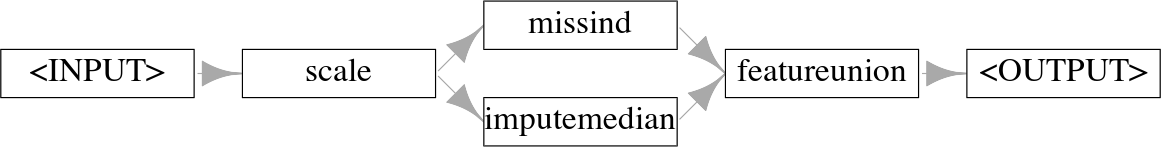
\includegraphics[width=1\textwidth,height=\textheight]{chapters/chapter8/non-sequential_pipelines_and_tuning_files/figure-pdf/fig-pipelines-parallel-plot-1.png}

}

\caption{\label{fig-pipelines-parallel-plot}Simple parallel pipeline
plot showing a common data source being scaled then the same data being
passed to two \texttt{PipeOp}s in parallel whose outputs are combined
and returned to the user.}

\end{figure}

When applied to the first three rows of the \texttt{"pima"} task we can
see how this imputes missing data and adds a column indicating where
values were missing.

\begin{Shaded}
\begin{Highlighting}[]
\NormalTok{tsk\_pima\_head }\OtherTok{=} \FunctionTok{tsk}\NormalTok{(}\StringTok{"pima"}\NormalTok{)}\SpecialCharTok{$}\FunctionTok{filter}\NormalTok{(}\DecValTok{1}\SpecialCharTok{:}\DecValTok{3}\NormalTok{)}
\NormalTok{tsk\_pima\_head}\SpecialCharTok{$}\FunctionTok{data}\NormalTok{(}\AttributeTok{cols =} \FunctionTok{c}\NormalTok{(}\StringTok{"diabetes"}\NormalTok{, }\StringTok{"insulin"}\NormalTok{, }\StringTok{"triceps"}\NormalTok{))}
\end{Highlighting}
\end{Shaded}

\begin{verbatim}
   diabetes insulin triceps
1:      pos      NA      35
2:      neg      NA      29
3:      pos      NA      NA
\end{verbatim}

\begin{Shaded}
\begin{Highlighting}[]
\NormalTok{result }\OtherTok{=}\NormalTok{ graph}\SpecialCharTok{$}\FunctionTok{train}\NormalTok{(tsk\_pima\_head)[[}\DecValTok{1}\NormalTok{]]}
\NormalTok{result}\SpecialCharTok{$}\FunctionTok{data}\NormalTok{(}\AttributeTok{cols =} \FunctionTok{c}\NormalTok{(}\StringTok{"diabetes"}\NormalTok{, }\StringTok{"insulin"}\NormalTok{, }\StringTok{"missing\_insulin"}\NormalTok{, }\StringTok{"triceps"}\NormalTok{,}
  \StringTok{"missing\_triceps"}\NormalTok{))}
\end{Highlighting}
\end{Shaded}

\begin{verbatim}
   diabetes insulin missing_insulin triceps missing_triceps
1:      pos       0         missing       3         present
2:      neg       0         missing      -3         present
3:      pos       0         missing       0         missing
\end{verbatim}

\hypertarget{selectors-and-parallel-pipelines}{%
\section{Selectors and Parallel
Pipelines}\label{selectors-and-parallel-pipelines}}

It is common in
\href{https://mlr3pipelines.mlr-org.com/reference/Graph.html}{\texttt{Graph}}s
for an operation to be applied to a subset of features. In
\texttt{mlr3pipelines} this can be achieved in two ways
(Figure~\ref{fig-pipelines-select-affect}): either by passing the column
subset to the \texttt{affect\_columns} hyperparameter of a
\href{https://mlr3pipelines.mlr-org.com/reference/PipeOp.html}{\texttt{PipeOp}}
(assuming it has that hyperparameter), which controls which columns
should be affected by the \texttt{PipeOp}; or, one can use the
\href{https://mlr3pipelines.mlr-org.com/reference/mlr_pipeops_select.html}{\texttt{PipeOpSelect}}\index{\texttt{PipeOpSelect}}
operator to create operations in parallel on specified feature subsets,
and then unite the result using
\href{https://mlr3pipelines.mlr-org.com/reference/mlr_pipeops_featureunion.html}{\texttt{PipeOpFeatureUnion}}.

\begin{figure}

\begin{minipage}[t]{\linewidth}

{\centering 

\raisebox{-\height}{


\includegraphics{chapters/chapter8/Figures/mlr3book_figures-28.png}

}

}

\subcaption{\label{fig-pipelines-select-affect-1}The
\texttt{affect\_columns} hyperparameter can be used to restrict
operations to a subset of features. When used, pipelines may still be
run in sequence.}
\end{minipage}%
\newline
\begin{minipage}[t]{\linewidth}

{\centering 

\raisebox{-\height}{

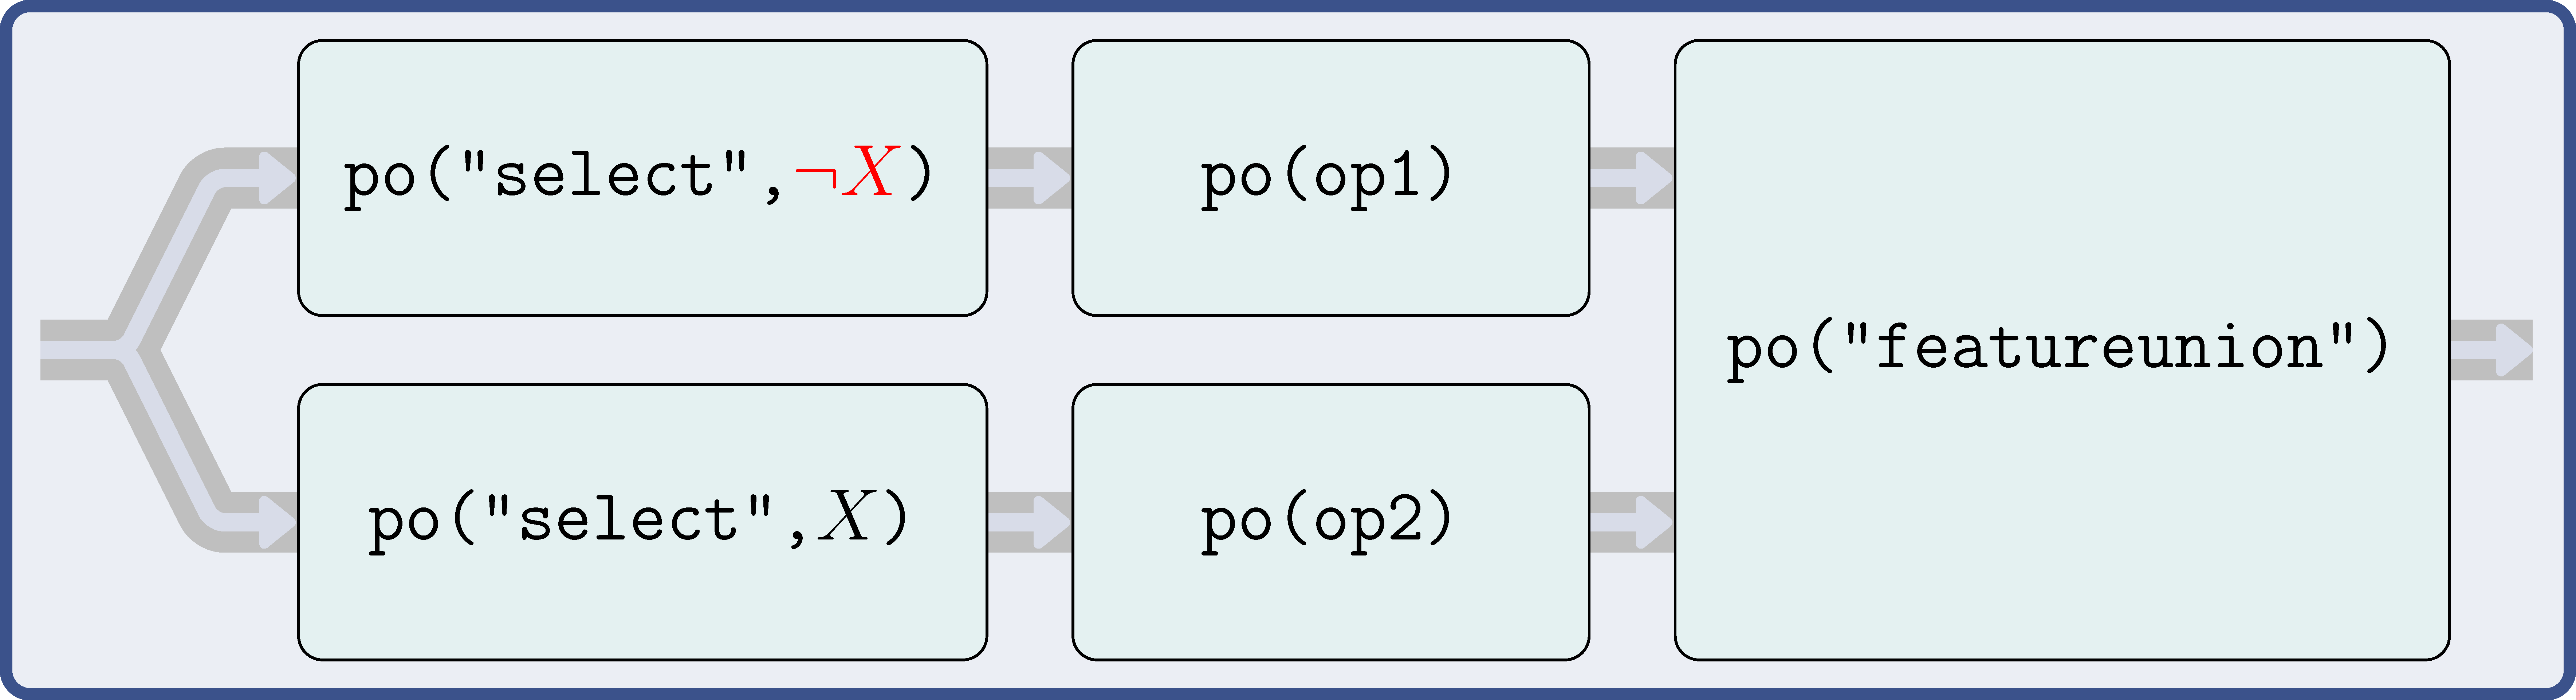
\includegraphics{chapters/chapter8/Figures/mlr3book_figures-29.png}

}

}

\subcaption{\label{fig-pipelines-select-affect-2}Operating on subsets of
tasks using concurrent paths by first splitting the inputs with
\texttt{po("select")} and then combining outputs with
\texttt{po("featureunion")}.}
\end{minipage}%

\caption{\label{fig-pipelines-select-affect}Two methods of setting up
\texttt{PipeOp}s (\texttt{po(op1)} and \texttt{po(op2)}) that operate on
complementary features (X and ¬X) of an input task.}

\end{figure}

Both methods make use of
\href{https://mlr3pipelines.mlr-org.com/reference/Selector.html}{\texttt{Selector}}\index{\texttt{Selector}}{\marginnote{\begin{footnotesize}\texttt{Selector}\end{footnotesize}}}-functions.
These are helper functions that indicate to a \texttt{PipeOp} which
features it should apply to. \texttt{Selectors} may match column names
by regular expressions
(\href{https://mlr3pipelines.mlr-org.com/reference/Selector.html}{\texttt{selector\_grep()}}),
or by column type
(\href{https://mlr3pipelines.mlr-org.com/reference/Selector.html}{\texttt{selector\_type()}}).
\texttt{Selectors} can also be used to join variables
(\href{https://mlr3pipelines.mlr-org.com/reference/Selector.html}{\texttt{selector\_union()}}),
return their set difference
(\href{https://mlr3pipelines.mlr-org.com/reference/Selector.html}{\texttt{selector\_setdiff()}}),
or select the complement of features from another \texttt{Selector}
(\href{https://mlr3pipelines.mlr-org.com/reference/Selector.html}{\texttt{selector\_invert()}}).

For example, in Section~\ref{sec-pipelines-pipeops} we applied PCA to
the bill length and depth of penguins from
\texttt{tsk("penguins\_simple")} by first selecting these columns using
the \texttt{Task} method \texttt{\$select()} and then applying the
\texttt{PipeOp}. We can now do this more simply with
\texttt{selector\_grep}, and could go on to use
\texttt{selector\_invert} to apply some other \texttt{PipeOp} to other
features, below we use \texttt{po("scale")} and make use of the
\texttt{affect\_columns} hyperparameter:

\begin{Shaded}
\begin{Highlighting}[]
\NormalTok{sel\_bill }\OtherTok{=} \FunctionTok{selector\_grep}\NormalTok{(}\StringTok{"\^{}bill"}\NormalTok{)}
\NormalTok{sel\_not\_bill }\OtherTok{=} \FunctionTok{selector\_invert}\NormalTok{(sel\_bill)}

\NormalTok{graph }\OtherTok{=} \FunctionTok{po}\NormalTok{(}\StringTok{"scale"}\NormalTok{, }\AttributeTok{affect\_columns =}\NormalTok{ sel\_not\_bill) }\SpecialCharTok{\%\textgreater{}\textgreater{}\%}
  \FunctionTok{po}\NormalTok{(}\StringTok{"pca"}\NormalTok{, }\AttributeTok{affect\_columns =}\NormalTok{ sel\_bill)}

\NormalTok{result }\OtherTok{=}\NormalTok{ graph}\SpecialCharTok{$}\FunctionTok{train}\NormalTok{(}\FunctionTok{tsk}\NormalTok{(}\StringTok{"penguins\_simple"}\NormalTok{))}
\NormalTok{result[[}\DecValTok{1}\NormalTok{]]}\SpecialCharTok{$}\FunctionTok{data}\NormalTok{()[}\DecValTok{1}\SpecialCharTok{:}\DecValTok{3}\NormalTok{, }\DecValTok{1}\SpecialCharTok{:}\DecValTok{5}\NormalTok{]}
\end{Highlighting}
\end{Shaded}

\begin{verbatim}
   species    PC1     PC2 body_mass flipper_length
1:  Adelie -5.015  1.0717   -0.5676        -1.4246
2:  Adelie -4.495 -0.1853   -0.5055        -1.0679
3:  Adelie -3.755  0.4868   -1.1886        -0.4257
\end{verbatim}

The biggest advantage of this method is that it creates a very simple,
sequential \texttt{Graph}. However, one disadvantage of the
\texttt{affect\_columns} method is that it is relatively easy to have
unexpected results if the ordering of \texttt{PipeOp}s is mixed up. For
example, if we had reversed the order of \texttt{po("pca")} and
\texttt{po("scale")} above then we would have first created columns
\texttt{"PC1"} and \texttt{"PC2"} and then erroneously scaled these,
since their names do not start with ``bill'' and they are therefore
matched by \texttt{sel\_not\_bill}. Creating parallel paths with
\texttt{po("select")} can help mitigate such errors by selecting
features given by the \texttt{Selector} and creating independent data
processing streams with the given feature subset. Below we pass the
parallel pipelines to
\href{https://mlr3pipelines.mlr-org.com/reference/gunion.html}{\texttt{gunion()}}
as a \texttt{list} to ensure they receive the same input, and then
combine the outputs with \texttt{po("featureunion")}.

\begin{Shaded}
\begin{Highlighting}[]
\NormalTok{po\_select\_bill }\OtherTok{=} \FunctionTok{po}\NormalTok{(}\StringTok{"select"}\NormalTok{, }\AttributeTok{id =} \StringTok{"s\_bill"}\NormalTok{, }\AttributeTok{selector =}\NormalTok{ sel\_bill)}
\NormalTok{po\_select\_not\_bill }\OtherTok{=} \FunctionTok{po}\NormalTok{(}\StringTok{"select"}\NormalTok{, }\AttributeTok{id =} \StringTok{"s\_notbill"}\NormalTok{,}
  \AttributeTok{selector =}\NormalTok{ sel\_not\_bill)}

\NormalTok{path\_pca }\OtherTok{=}\NormalTok{  po\_select\_bill }\SpecialCharTok{\%\textgreater{}\textgreater{}\%} \FunctionTok{po}\NormalTok{(}\StringTok{"pca"}\NormalTok{)}
\NormalTok{path\_scale }\OtherTok{=}\NormalTok{ po\_select\_not\_bill }\SpecialCharTok{\%\textgreater{}\textgreater{}\%} \FunctionTok{po}\NormalTok{(}\StringTok{"scale"}\NormalTok{)}

\NormalTok{graph }\OtherTok{=} \FunctionTok{gunion}\NormalTok{(}\FunctionTok{list}\NormalTok{(path\_pca, path\_scale)) }\SpecialCharTok{\%\textgreater{}\textgreater{}\%} \FunctionTok{po}\NormalTok{(}\StringTok{"featureunion"}\NormalTok{)}
\NormalTok{graph}\SpecialCharTok{$}\FunctionTok{plot}\NormalTok{(}\AttributeTok{horizontal =} \ConstantTok{TRUE}\NormalTok{)}
\end{Highlighting}
\end{Shaded}

\begin{figure}

{\centering 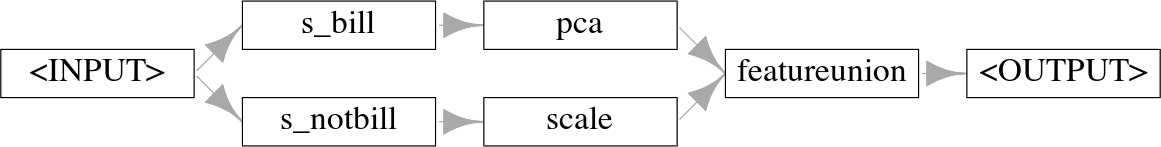
\includegraphics[width=1\textwidth,height=\textheight]{chapters/chapter8/non-sequential_pipelines_and_tuning_files/figure-pdf/fig-pipelines-pcascale-1.png}

}

\caption{\label{fig-pipelines-pcascale}Visualization of a \texttt{Graph}
where features are split into two paths, one with PCA and one with
scaling, then combined and returned.}

\end{figure}

The \texttt{po("select")} method also has the significant advantage that
it allows the same set of features to be used in multiple operations
simultaneously, or to both transform features and keep their
untransformed versions (by using \texttt{po("nop")} in one path).
\href{https://mlr3pipelines.mlr-org.com/reference/mlr_pipeops_nop.html}{\texttt{PipeOpNOP}}
performs no operation on its inputs and is thus useful when you only
want to perform a transformation on a subset of features and leave the
others untouched:

\begin{Shaded}
\begin{Highlighting}[]
\NormalTok{graph }\OtherTok{=} \FunctionTok{gunion}\NormalTok{(}\FunctionTok{list}\NormalTok{(}
\NormalTok{  po\_select\_bill }\SpecialCharTok{\%\textgreater{}\textgreater{}\%} \FunctionTok{po}\NormalTok{(}\StringTok{"scale"}\NormalTok{),}
\NormalTok{  po\_select\_not\_bill }\SpecialCharTok{\%\textgreater{}\textgreater{}\%} \FunctionTok{po}\NormalTok{(}\StringTok{"nop"}\NormalTok{)}
\NormalTok{)) }\SpecialCharTok{\%\textgreater{}\textgreater{}\%} \FunctionTok{po}\NormalTok{(}\StringTok{"featureunion"}\NormalTok{)}
\NormalTok{graph}\SpecialCharTok{$}\FunctionTok{plot}\NormalTok{(}\AttributeTok{horizontal =} \ConstantTok{TRUE}\NormalTok{)}
\end{Highlighting}
\end{Shaded}

\begin{figure}

{\centering \includegraphics[width=1\textwidth,height=\textheight]{chapters/chapter8/non-sequential_pipelines_and_tuning_files/figure-pdf/fig-pipelines-selectnop-1.png}

}

\caption{\label{fig-pipelines-selectnop}Visualization of our
\texttt{Graph} where features are split into two paths, features that
start with `bill' are scaled and the rest are untransformed.}

\end{figure}

\begin{Shaded}
\begin{Highlighting}[]
\NormalTok{graph}\SpecialCharTok{$}\FunctionTok{train}\NormalTok{(}\FunctionTok{tsk}\NormalTok{(}\StringTok{"penguins\_simple"}\NormalTok{))[[}\DecValTok{1}\NormalTok{]]}\SpecialCharTok{$}\FunctionTok{data}\NormalTok{()[}\DecValTok{1}\SpecialCharTok{:}\DecValTok{3}\NormalTok{, }\DecValTok{1}\SpecialCharTok{:}\DecValTok{5}\NormalTok{]}
\end{Highlighting}
\end{Shaded}

\begin{verbatim}
   species bill_depth bill_length body_mass flipper_length
1:  Adelie     0.7796     -0.8947      3750            181
2:  Adelie     0.1194     -0.8216      3800            186
3:  Adelie     0.4241     -0.6753      3250            195
\end{verbatim}

\hypertarget{sec-pipelines-ppl}{%
\section{Common Patterns and ppl()}\label{sec-pipelines-ppl}}

Now you have the tools to create sequential and non-sequential
pipelines, you can create an infinite number of transformations on
\href{https://mlr3.mlr-org.com/reference/Task.html}{\texttt{Task}},
\href{https://mlr3.mlr-org.com/reference/Learner.html}{\texttt{Learner}},
and
\href{https://mlr3.mlr-org.com/reference/Prediction.html}{\texttt{Prediction}}
objects. In Section~\ref{sec-pipelines-bagging} and
Section~\ref{sec-pipelines-stack} we will work through two examples to
demonstrate how you can make complex and powerful graphs using the
methods and classes we have already looked at. However, many common
problems in ML can be well solved by the same pipelines, and so to make
your life easier we have implemented and saved these pipelines in the
\href{https://mlr3pipelines.mlr-org.com/reference/mlr_graphs.html}{\texttt{mlr\_graphs}}\index{\texttt{mlr\_graphs}}
dictionary; pipelines in the dictionary can be accessed with the
\href{https://mlr3pipelines.mlr-org.com/reference/ppl.html}{\texttt{ppl()}}\index{\texttt{ppl()}}{\marginnote{\begin{footnotesize}\texttt{ppl()}\end{footnotesize}}}
sugar function.

At the time of writing, this dictionary includes seven
\href{https://mlr3pipelines.mlr-org.com/reference/Graph.html}{\texttt{Graph}}s
(required arguments included below):

\begin{itemize}
\tightlist
\item
  \texttt{ppl("bagging",\ graph)}: In \texttt{mlr3pipelines},
  bagging\index{bagging} is the process of running a \texttt{graph}
  multiple times on different data samples and then averaging the
  results. This is discussed in detail in
  Section~\ref{sec-pipelines-bagging}.
\item
  \texttt{ppl("branch",\ graphs)}: Uses
  \href{https://mlr3pipelines.mlr-org.com/reference/mlr_pipeops_branch.html}{\texttt{PipeOpBranch}}
  to create different path branches from the given \texttt{graphs} where
  only one branch is evaluated. This is returned to in more detail in
  Section~\ref{sec-pipelines-branch}.
\item
  \texttt{ppl("greplicate",\ graph,\ n)}: Create a \texttt{Graph} that
  replicates \texttt{graph} (which can also be a single \texttt{PipeOp})
  \texttt{n} times. The pipeline avoids ID clashes by adding a suffix to
  each \texttt{PipeOp}, we will see this pipeline in use in
  Section~\ref{sec-pipelines-bagging}.
\item
  \texttt{ppl("ovr",\ graph)}: One-versus-rest
  classification\index{one-versus-rest classification} for converting
  multiclass classification\index{classification!multiclass} tasks into
  several binary classification tasks with one task for each class in
  the original. These tasks are then evaluated by the given
  \texttt{graph}, which should be a learner (or a pipeline containing a
  learner that emits a prediction). The predictions made on the binary
  tasks are combined into the multiclass prediction needed for the
  original task.
\item
  \texttt{ppl("robustify")}: Performs common preprocessing steps to make
  any \texttt{Task} compatible with a given \texttt{Learner}. This
  pipeline is demonstrated in Section~\ref{sec-prepro-robustify}.
\item
  \texttt{ppl("stacking",\ base\_learners,\ super\_learner)}:
  Stacking\index{stacking}, returned to in detail in
  Section~\ref{sec-pipelines-stack}, is the process of using predictions
  from one or more models (\texttt{base\_learners}) as features in a
  subsequent model (\texttt{super\_learner})
\item
  \texttt{ppl("targettrafo",\ graph)}: Create a \texttt{Graph} that
  transforms the prediction target of a task and ensures that any
  transformations applied during training (using the function passed to
  the \texttt{targetmutate.trafo} hyperparameter) are inverted in the
  resulting predictions (using the function passed to the
  \texttt{targetmutate.inverter} hyperparameter); an example is given in
  Section~\ref{sec-prepro-scale}.
\end{itemize}

\hypertarget{practical-pipelines-by-example}{%
\section{Practical Pipelines by
Example}\label{practical-pipelines-by-example}}

In this section, we will put pipelines into practice by demonstrating
how to turn weak learners into powerful machine learning models using
bagging\index{bagging} and stacking\index{stacking}.

\hypertarget{sec-pipelines-bagging}{%
\subsection{Bagging with ``greplicate'' and
``subsample''}\label{sec-pipelines-bagging}}

The basic idea of bagging\index{bagging} (from \textbf{b}ootstrapp
\textbf{agg}regat\textbf{ing}), introduced by Breiman (1996), is to
aggregate multiple predictors into a single, more powerful predictor
(Figure~\ref{fig-pipelines-bagging}). Predictions are usually aggregated
by the arithmetic mean for regression tasks or majority vote for
classification. The underlying intuition behind bagging is that
averaging a set of unstable and diverse (i.e., only weakly correlated)
predictors can reduce the variance of the overall prediction. Each
learner is trained on a different random sample of the original data.

Although we have already seen that a pre-constructed bagging pipeline is
available with \texttt{ppl("bagging")}, in this section we will build
our own pipeline from scratch to showcase how to construct a complex
\href{https://mlr3pipelines.mlr-org.com/reference/Graph.html}{\texttt{Graph}},
which will look something like Figure~\ref{fig-pipelines-bagging}.

\begin{figure}

{\centering \includegraphics[width=0.7\textwidth,height=\textheight]{chapters/chapter8/Figures/mlr3book_figures-26.png}

}

\caption{\label{fig-pipelines-bagging}Graph that performs Bagging by
independently subsampling data and fitting individual decision tree
learners. The resulting predictions are aggregated by a majority vote
\texttt{PipeOp}.}

\end{figure}

To begin, we use \texttt{po("subsample")} to sample a fraction of the
data (here 70\%), which is then passed to a classification tree (note by
default \texttt{po("subsample")} samples without replacement).

\begin{Shaded}
\begin{Highlighting}[]
\NormalTok{gr\_single\_pred }\OtherTok{=} \FunctionTok{po}\NormalTok{(}\StringTok{"subsample"}\NormalTok{, }\AttributeTok{frac =} \FloatTok{0.7}\NormalTok{) }\SpecialCharTok{\%\textgreater{}\textgreater{}\%} \FunctionTok{lrn}\NormalTok{(}\StringTok{"classif.rpart"}\NormalTok{)}
\end{Highlighting}
\end{Shaded}

Next, we use \texttt{ppl("greplicate")} to copy the graph,
\texttt{gr\_single\_pred}, 10 times (\texttt{n\ =\ 10}) and finally
\texttt{po("classifavg")} to take the majority vote of all predictions,
note that we pass \texttt{innum\ =\ 10} to \texttt{"classifavg"} to tell
the
\href{https://mlr3pipelines.mlr-org.com/reference/PipeOp.html}{\texttt{PipeOp}}
to expect 10 inputs.

\begin{Shaded}
\begin{Highlighting}[]
\NormalTok{gr\_pred\_set }\OtherTok{=} \FunctionTok{ppl}\NormalTok{(}\StringTok{"greplicate"}\NormalTok{, }\AttributeTok{graph =}\NormalTok{ gr\_single\_pred, }\AttributeTok{n =} \DecValTok{10}\NormalTok{)}
\NormalTok{gr\_bagging }\OtherTok{=}\NormalTok{ gr\_pred\_set }\SpecialCharTok{\%\textgreater{}\textgreater{}\%} \FunctionTok{po}\NormalTok{(}\StringTok{"classifavg"}\NormalTok{, }\AttributeTok{innum =} \DecValTok{10}\NormalTok{)}
\NormalTok{gr\_bagging}\SpecialCharTok{$}\FunctionTok{plot}\NormalTok{()}
\end{Highlighting}
\end{Shaded}

\begin{figure}

{\centering \includegraphics[width=1\textwidth,height=\textheight]{chapters/chapter8/non-sequential_pipelines_and_tuning_files/figure-pdf/fig-pipelines-bagginggraph-1.png}

}

\caption{\label{fig-pipelines-bagginggraph}Constructed bagging
\texttt{Graph} with one input being sampled many times for 10 different
learners.}

\end{figure}

Now let us see how well our bagging pipeline compares to the single
decision tree and a random forest when benchmarked against
\texttt{tsk("sonar")}.

\begin{Shaded}
\begin{Highlighting}[]
\CommentTok{\# turn graph into learner}
\NormalTok{glrn\_bagging }\OtherTok{=} \FunctionTok{as\_learner}\NormalTok{(gr\_bagging)}
\NormalTok{glrn\_bagging}\SpecialCharTok{$}\NormalTok{id }\OtherTok{=} \StringTok{"bagging"}

\NormalTok{lrn\_rpart }\OtherTok{=} \FunctionTok{lrn}\NormalTok{(}\StringTok{"classif.rpart"}\NormalTok{)}
\NormalTok{learners }\OtherTok{=} \FunctionTok{c}\NormalTok{(glrn\_bagging, lrn\_rpart, }\FunctionTok{lrn}\NormalTok{(}\StringTok{"classif.ranger"}\NormalTok{))}

\NormalTok{bmr }\OtherTok{=} \FunctionTok{benchmark}\NormalTok{(}\FunctionTok{benchmark\_grid}\NormalTok{(}\FunctionTok{tsk}\NormalTok{(}\StringTok{"sonar"}\NormalTok{), learners,}
  \FunctionTok{rsmp}\NormalTok{(}\StringTok{"cv"}\NormalTok{, }\AttributeTok{folds =} \DecValTok{3}\NormalTok{)))}
\NormalTok{bmr}\SpecialCharTok{$}\FunctionTok{aggregate}\NormalTok{()[, .(learner\_id, classif.ce)]}
\end{Highlighting}
\end{Shaded}

\begin{verbatim}
       learner_id classif.ce
1:        bagging     0.2498
2:  classif.rpart     0.2739
3: classif.ranger     0.2021
\end{verbatim}

The bagged learner performs better than the decision tree but worse than
the random forest. To automatically recreate this pipeline, you can
construct \texttt{ppl("bagging")} by specifying the learner to `bag',
the number of iterations, the fraction of data to sample, and the
\href{https://mlr3pipelines.mlr-org.com/reference/PipeOp.html}{\texttt{PipeOp}}
to average the predictions, as shown in the code below. Note we set
\texttt{collect\_multiplicity\ =\ TRUE} which collects the predictions
across paths, that technically use the
\href{https://mlr3pipelines.mlr-org.com/reference/Multiplicity.html}{\texttt{Multiplicity}}
method, which we will not discuss here but refer the reader to the
documentation.

\begin{Shaded}
\begin{Highlighting}[]
\FunctionTok{ppl}\NormalTok{(}\StringTok{"bagging"}\NormalTok{, }\FunctionTok{lrn}\NormalTok{(}\StringTok{"classif.rpart"}\NormalTok{),}
  \AttributeTok{iterations =} \DecValTok{10}\NormalTok{, }\AttributeTok{frac =} \FloatTok{0.7}\NormalTok{,}
  \AttributeTok{averager =} \FunctionTok{po}\NormalTok{(}\StringTok{"classifavg"}\NormalTok{, }\AttributeTok{collect\_multiplicity =} \ConstantTok{TRUE}\NormalTok{))}
\end{Highlighting}
\end{Shaded}

The main difference between our pipeline and a random forest is that the
latter also performs feature subsampling, where only a random subset of
available features is considered at each split point. While we cannot
implement this directly with \texttt{mlr3pipelines}, we can use a custom
\href{https://mlr3pipelines.mlr-org.com/reference/Selector.html}{\texttt{Selector}}
method to approximate this method. We will create this \texttt{Selector}
by passing a function that takes as input the task and returns a sample
of the features, we sample the square root of the number of features to
mimic the implementation in
\href{https://www.rdocumentation.org/packages/ranger/topics/ranger}{\texttt{ranger}}.
For efficiency, we will now use \texttt{ppl("bagging")} to recreate the
steps above:

\begin{Shaded}
\begin{Highlighting}[]
\CommentTok{\# custom selector}
\NormalTok{selector\_subsample }\OtherTok{=} \ControlFlowTok{function}\NormalTok{(task) \{}
  \FunctionTok{sample}\NormalTok{(task}\SpecialCharTok{$}\NormalTok{feature\_names, }\FunctionTok{sqrt}\NormalTok{(}\FunctionTok{length}\NormalTok{(task}\SpecialCharTok{$}\NormalTok{feature\_names)))}
\NormalTok{\}}

\CommentTok{\# bagging pipeline with our selector}
\NormalTok{gr\_bagging\_quasi\_rf }\OtherTok{=} \FunctionTok{ppl}\NormalTok{(}\StringTok{"bagging"}\NormalTok{,}
  \AttributeTok{graph =} \FunctionTok{po}\NormalTok{(}\StringTok{"select"}\NormalTok{, }\AttributeTok{selector =}\NormalTok{ selector\_subsample) }\SpecialCharTok{\%\textgreater{}\textgreater{}\%}
    \FunctionTok{lrn}\NormalTok{(}\StringTok{"classif.rpart"}\NormalTok{, }\AttributeTok{minsplit =} \DecValTok{1}\NormalTok{),}
  \AttributeTok{iterations =} \DecValTok{100}\NormalTok{,}
  \AttributeTok{averager =} \FunctionTok{po}\NormalTok{(}\StringTok{"classifavg"}\NormalTok{, }\AttributeTok{collect\_multiplicity =} \ConstantTok{TRUE}\NormalTok{)}
\NormalTok{)}

\CommentTok{\# bootstrap resampling}
\NormalTok{gr\_bagging\_quasi\_rf}\SpecialCharTok{$}\NormalTok{param\_set}\SpecialCharTok{$}\NormalTok{values}\SpecialCharTok{$}\NormalTok{subsample.replace }\OtherTok{=} \ConstantTok{TRUE}

\CommentTok{\# convert to learner}
\NormalTok{glrn\_quasi\_rf }\OtherTok{=} \FunctionTok{as\_learner}\NormalTok{(gr\_bagging\_quasi\_rf)}
\NormalTok{glrn\_quasi\_rf}\SpecialCharTok{$}\NormalTok{id }\OtherTok{=} \StringTok{"quasi.rf"}

\CommentTok{\# benchmark}
\NormalTok{design }\OtherTok{=} \FunctionTok{benchmark\_grid}\NormalTok{(}\FunctionTok{tsks}\NormalTok{(}\StringTok{"sonar"}\NormalTok{),}
  \FunctionTok{c}\NormalTok{(glrn\_quasi\_rf, }\FunctionTok{lrn}\NormalTok{(}\StringTok{"classif.ranger"}\NormalTok{, }\AttributeTok{num.trees =} \DecValTok{100}\NormalTok{)),}
  \FunctionTok{rsmp}\NormalTok{(}\StringTok{"cv"}\NormalTok{, }\AttributeTok{folds =} \DecValTok{5}\NormalTok{)}
\NormalTok{)}
\NormalTok{bmr }\OtherTok{=} \FunctionTok{benchmark}\NormalTok{(design)}
\NormalTok{bmr}\SpecialCharTok{$}\FunctionTok{aggregate}\NormalTok{()[, .(learner\_id, classif.ce)]}
\end{Highlighting}
\end{Shaded}

\begin{verbatim}
       learner_id classif.ce
1:       quasi.rf     0.1826
2: classif.ranger     0.1779
\end{verbatim}

In only a few lines of code, we took a weaker learner and turned it into
a powerful model that we can see is comparable to the implementation in
\texttt{ranger::ranger}. In the next section, we will look at a second
example, which makes use of cross-validation within pipelines.

\hypertarget{sec-pipelines-stack}{%
\subsection{Stacking with
po(``learner\_cv'')}\label{sec-pipelines-stack}}

Stacking\index{stacking} (Wolpert 1992) is another very popular
ensembling technique that can significantly improve predictive
performance. The basic idea behind stacking is to use predictions from
multiple models (usually referred to as level 0 models) as features for
a subsequent model (the level 1 model) which in turn combines these
predictions (Figure~\ref{fig-pipelines-stacking}). A simple combination
can be a linear model (possibly regularized if you have many level 0
models), since a weighted sum of level 0 models is often plausible and
good enough. Though, non-linear level 1 models can also be used, and it
is also possible for the level 1 model to access the input features as
well as the level 0 predictions. Stacking can be built with more than
two levels (both conceptually, and in \texttt{mlr3}) but we limit
ourselves to this simpler setup here, which often also performs well in
practice.

As with bagging, we will demonstrate how to create a stacking pipeline
manually, although a pre-constructed pipeline is available with
\texttt{ppl("stacking")}.

\begin{figure}

{\centering \includegraphics[width=0.7\textwidth,height=\textheight]{chapters/chapter8/Figures/mlr3book_figures-27.png}

}

\caption{\label{fig-pipelines-stacking}Graph that performs Stacking by
fitting three models and using their outputs as features for another
model after combining with \texttt{PipeOpFeatureUnion}.}

\end{figure}

Stacking pipelines depend on the level 0 learners returning predictions
during the \texttt{\$train()} phase. This is possible in
\texttt{mlr3pipelines} with
\href{https://mlr3pipelines.mlr-org.com/reference/mlr_pipeops_learner_cv.html}{\texttt{PipeOpLearnerCV}}\index{\texttt{PipeOpLearnerCV}}.
During training, this operator performs cross-validation and passes the
out-of-sample predictions to the level 1 model. Using cross-validated
predictions is recommended to reduce the risk of overfitting.

We first create the level 0 learners to produce the predictions that
will be used as features. In this example, we use a classification
tree\index{decision tree}, k-nearest
neighbors\index{k-nearest neighbors}
(KNN)\index{KNN|see{k-nearest neighbors}}, and a regularized
GLM\index{generalized linear model}. Each learner is wrapped in
\texttt{po("learner\_cv")} which performs cross-validation on the input
data and then outputs the predictions from the
\href{https://mlr3.mlr-org.com/reference/Learner.html}{\texttt{Learner}}
in a new
\href{https://mlr3.mlr-org.com/reference/Task.html}{\texttt{Task}}
object.

\begin{Shaded}
\begin{Highlighting}[]
\NormalTok{lrn\_rpart }\OtherTok{=} \FunctionTok{lrn}\NormalTok{(}\StringTok{"classif.rpart"}\NormalTok{, }\AttributeTok{predict\_type =} \StringTok{"prob"}\NormalTok{)}
\NormalTok{po\_rpart\_cv }\OtherTok{=} \FunctionTok{po}\NormalTok{(}\StringTok{"learner\_cv"}\NormalTok{, }\AttributeTok{learner =}\NormalTok{ lrn\_rpart,}
  \AttributeTok{resampling.folds =} \DecValTok{2}\NormalTok{, }\AttributeTok{id =} \StringTok{"rpart\_cv"}
\NormalTok{)}

\NormalTok{lrn\_knn }\OtherTok{=} \FunctionTok{lrn}\NormalTok{(}\StringTok{"classif.kknn"}\NormalTok{, }\AttributeTok{predict\_type =} \StringTok{"prob"}\NormalTok{)}
\NormalTok{po\_knn\_cv }\OtherTok{=} \FunctionTok{po}\NormalTok{(}\StringTok{"learner\_cv"}\NormalTok{,}
  \AttributeTok{learner =}\NormalTok{ lrn\_knn,}
  \AttributeTok{resampling.folds =} \DecValTok{2}\NormalTok{, }\AttributeTok{id =} \StringTok{"knn\_cv"}
\NormalTok{)}

\NormalTok{lrn\_glmnet }\OtherTok{=} \FunctionTok{lrn}\NormalTok{(}\StringTok{"classif.glmnet"}\NormalTok{, }\AttributeTok{predict\_type =} \StringTok{"prob"}\NormalTok{)}
\NormalTok{po\_glmnet\_cv }\OtherTok{=} \FunctionTok{po}\NormalTok{(}\StringTok{"learner\_cv"}\NormalTok{,}
  \AttributeTok{learner =}\NormalTok{ lrn\_glmnet,}
  \AttributeTok{resampling.folds =} \DecValTok{2}\NormalTok{, }\AttributeTok{id =} \StringTok{"glmnet\_cv"}
\NormalTok{)}
\end{Highlighting}
\end{Shaded}

These learners are combined using
\href{https://mlr3pipelines.mlr-org.com/reference/gunion.html}{\texttt{gunion()}},
and \texttt{po("featureunion")} is used to merge their predictions. This
is demonstrated in the output of \texttt{\$train()}:

\begin{Shaded}
\begin{Highlighting}[]
\NormalTok{gr\_level\_0 }\OtherTok{=} \FunctionTok{gunion}\NormalTok{(}\FunctionTok{list}\NormalTok{(po\_rpart\_cv, po\_knn\_cv, po\_glmnet\_cv))}
\NormalTok{gr\_combined }\OtherTok{=}\NormalTok{ gr\_level\_0 }\SpecialCharTok{\%\textgreater{}\textgreater{}\%} \FunctionTok{po}\NormalTok{(}\StringTok{"featureunion"}\NormalTok{)}

\NormalTok{gr\_combined}\SpecialCharTok{$}\FunctionTok{train}\NormalTok{(}\FunctionTok{tsk}\NormalTok{(}\StringTok{"sonar"}\NormalTok{))[[}\DecValTok{1}\NormalTok{]]}\SpecialCharTok{$}\FunctionTok{head}\NormalTok{()}
\end{Highlighting}
\end{Shaded}

\begin{verbatim}
   Class rpart_cv.prob.M rpart_cv.prob.R knn_cv.prob.M knn_cv.prob.R
1:     R         0.57895          0.4211        0.3857        0.6143
2:     R         0.88636          0.1136        0.3170        0.6830
3:     R         0.04348          0.9565        0.4396        0.5604
4:     R         0.03030          0.9697        0.4762        0.5238
5:     R         0.04348          0.9565        0.4753        0.5247
6:     R         0.23077          0.7692        0.4020        0.5980
2 variables not shown: [glmnet_cv.prob.M, glmnet_cv.prob.R]
\end{verbatim}

\begin{tcolorbox}[enhanced jigsaw, opacitybacktitle=0.6, rightrule=.15mm, opacityback=0, arc=.35mm, breakable, titlerule=0mm, colframe=quarto-callout-tip-color-frame, coltitle=black, bottomrule=.15mm, toprule=.15mm, colback=white, colbacktitle=quarto-callout-tip-color!10!white, bottomtitle=1mm, toptitle=1mm, title=\textcolor{quarto-callout-tip-color}{\faLightbulb}\hspace{0.5em}{Retaining Features}, leftrule=.75mm, left=2mm]

In this example, the original features were removed as each
\texttt{PipeOp} only returns the predictions made by the respective
learners. To retain the original features, include \texttt{po("nop")} in
the list passed to
\href{https://mlr3pipelines.mlr-org.com/reference/gunion.html}{\texttt{gunion()}}.

\end{tcolorbox}

The resulting task contains the predicted probabilities for both classes
made from each of the level 0 learners. However, as the probabilities
always add up to \(1\), we only need the predictions for one of the
classes (as this is a binary classification task), so we can use
\texttt{po("select")} to only keep predictions for one class (we choose
\texttt{"M"} in this example).

\begin{Shaded}
\begin{Highlighting}[]
\NormalTok{gr\_stack }\OtherTok{=}\NormalTok{ gr\_combined }\SpecialCharTok{\%\textgreater{}\textgreater{}\%}
  \FunctionTok{po}\NormalTok{(}\StringTok{"select"}\NormalTok{, }\AttributeTok{selector =} \FunctionTok{selector\_grep}\NormalTok{(}\StringTok{"}\SpecialCharTok{\textbackslash{}\textbackslash{}}\StringTok{.M$"}\NormalTok{))}
\end{Highlighting}
\end{Shaded}

Finally, we can combine our pipeline with the final model that will take
these predictions as its input. Below we use logistic
regression\index{logistic regression}, which combines the level 0
predictions in a weighted linear sum.

\begin{Shaded}
\begin{Highlighting}[]
\NormalTok{gr\_stack }\OtherTok{=}\NormalTok{ gr\_stack }\SpecialCharTok{\%\textgreater{}\textgreater{}\%} \FunctionTok{po}\NormalTok{(}\StringTok{"learner"}\NormalTok{, }\FunctionTok{lrn}\NormalTok{(}\StringTok{"classif.log\_reg"}\NormalTok{))}
\NormalTok{gr\_stack}\SpecialCharTok{$}\FunctionTok{plot}\NormalTok{(}\AttributeTok{horizontal =} \ConstantTok{TRUE}\NormalTok{)}
\end{Highlighting}
\end{Shaded}

\begin{figure}

{\centering \includegraphics[width=1\textwidth,height=\textheight]{chapters/chapter8/non-sequential_pipelines_and_tuning_files/figure-pdf/fig-pipelines-stackinggraph-1.png}

}

\caption{\label{fig-pipelines-stackinggraph}Constructed stacking Graph
with one input being passed to three weak learners whose predictions are
passed to the logistic regression.}

\end{figure}

As our final model was an interpretable logistic regression, we can
inspect the weights of the level 0 learners by looking at the final
trained model:

\begin{Shaded}
\begin{Highlighting}[]
\NormalTok{glrn\_stack }\OtherTok{=} \FunctionTok{as\_learner}\NormalTok{(gr\_stack)}
\NormalTok{glrn\_stack}\SpecialCharTok{$}\FunctionTok{train}\NormalTok{(}\FunctionTok{tsk}\NormalTok{(}\StringTok{"sonar"}\NormalTok{))}
\NormalTok{glrn\_stack}\SpecialCharTok{$}\FunctionTok{base\_learner}\NormalTok{()}\SpecialCharTok{$}\NormalTok{model}
\end{Highlighting}
\end{Shaded}

\begin{verbatim}

Call:  stats::glm(formula = task$formula(), family = "binomial", data = data, 
    model = FALSE)

Coefficients:
     (Intercept)   rpart_cv.prob.M     knn_cv.prob.M  glmnet_cv.prob.M  
          -3.120            -0.134             4.040             1.804  

Degrees of Freedom: 207 Total (i.e. Null);  204 Residual
Null Deviance:      287 
Residual Deviance: 176  AIC: 184
\end{verbatim}

The model weights suggest that knn influences the predictions the most
with the largest coefficient. To confirm this we can benchmark the
individual models alongside the stacking pipeline.

\begin{Shaded}
\begin{Highlighting}[]
\NormalTok{glrn\_stack}\SpecialCharTok{$}\NormalTok{id }\OtherTok{=} \StringTok{"stacking"}
\NormalTok{design }\OtherTok{=} \FunctionTok{benchmark\_grid}\NormalTok{(}\FunctionTok{tsk}\NormalTok{(}\StringTok{"sonar"}\NormalTok{),}
  \FunctionTok{list}\NormalTok{(lrn\_rpart, lrn\_knn, lrn\_glmnet, glrn\_stack), }\FunctionTok{rsmp}\NormalTok{(}\StringTok{"repeated\_cv"}\NormalTok{))}
\NormalTok{bmr }\OtherTok{=} \FunctionTok{benchmark}\NormalTok{(design)}
\NormalTok{bmr}\SpecialCharTok{$}\FunctionTok{aggregate}\NormalTok{()[, .(learner\_id, classif.ce)]}
\end{Highlighting}
\end{Shaded}

\begin{verbatim}
       learner_id classif.ce
1:  classif.rpart     0.2876
2:   classif.kknn     0.1505
3: classif.glmnet     0.2559
4:       stacking     0.1438
\end{verbatim}

This experiment confirms that of the individual models, the KNN learner
performs the best, however, our stacking pipeline outperforms them all.
Now that we have seen the inner workings of this pipeline, next time you
might want to more efficiently create it using \texttt{ppl("stacking")},
to copy the example above you would run:

\begin{Shaded}
\begin{Highlighting}[]
\FunctionTok{ppl}\NormalTok{(}\StringTok{"stacking"}\NormalTok{,}
  \AttributeTok{base\_learners =} \FunctionTok{lrns}\NormalTok{(}\FunctionTok{c}\NormalTok{(}\StringTok{"classif.rpart"}\NormalTok{, }\StringTok{"classif.kknn"}\NormalTok{,}
    \StringTok{"classif.glmnet"}\NormalTok{)),}
  \AttributeTok{super\_learner =} \FunctionTok{lrn}\NormalTok{(}\StringTok{"classif.log\_reg"}\NormalTok{)}
\NormalTok{)}
\end{Highlighting}
\end{Shaded}

Having covered the building blocks of \texttt{mlr3pipelines} and seen
these in practice, we will now turn to more advanced functionality,
combining pipelines with tuning.

\hypertarget{sec-pipelines-tuning}{%
\section{\texorpdfstring{Tuning\index{tuning}
Graphs}{Tuning Graphs}}\label{sec-pipelines-tuning}}

By wrapping a pipeline inside a
\href{https://mlr3pipelines.mlr-org.com/reference/mlr_learners_graph.html}{\texttt{GraphLearner}},
we can tune it at two levels of complexity using
\href{https://mlr3tuning.mlr-org.com}{\texttt{mlr3tuning}}\index{\texttt{mlr3tuning}}:

\begin{enumerate}
\def\labelenumi{\arabic{enumi}.}
\item
  Tuning of a fixed, usually sequential pipeline, where preprocessing is
  combined with a given learner. This simply means the joint tuning of
  any subset of selected hyperparameters of operations in the pipeline.
  Conceptually and also technically in \texttt{mlr3}, this is not much
  different from tuning a learner that is not part of a pipeline.
\item
  Tuning not only the hyperparameters of a pipeline, whose structure is
  not completely fixed in terms of its included operations, but also
  which concrete
  \href{https://mlr3pipelines.mlr-org.com/reference/PipeOp.html}{\texttt{PipeOp}}s
  should be applied to data. This allows us to select these operations
  (e.g.~which learner to use, which preprocessing to perform) in a
  data-driven manner known as ``Combined Algorithm Selection and
  Hyperparameter
  optimization\index{combined algorithm selection and hyperparameter optimization}''\index{CASH|see{combined algorithm selection and hyperparameter optimization}}
  (Thornton et al. 2013). As we will soon see, we can do this in
  \texttt{mlr3pipelines} by using the powerful branching
  (Section~\ref{sec-pipelines-branch}) and proxy
  (Section~\ref{sec-pipelines-proxy}) meta operators. Through this, we
  can conveniently create our own ``mini AutoML systems'' (Hutter,
  Kotthoff, and Vanschoren 2019) in \texttt{mlr3}, which can even be
  geared for specific tasks.
\end{enumerate}

\hypertarget{sec-pipelines-combined}{%
\subsection{Tuning Graph Hyperparameters}\label{sec-pipelines-combined}}

Let us consider a simple, sequential pipeline using \texttt{po("pca")}
followed by \texttt{lrn("classif.kknn")}:

\begin{Shaded}
\begin{Highlighting}[]
\NormalTok{graph\_learner }\OtherTok{=} \FunctionTok{as\_learner}\NormalTok{(}\FunctionTok{po}\NormalTok{(}\StringTok{"pca"}\NormalTok{) }\SpecialCharTok{\%\textgreater{}\textgreater{}\%} \FunctionTok{lrn}\NormalTok{(}\StringTok{"classif.kknn"}\NormalTok{))}
\end{Highlighting}
\end{Shaded}

The optimal setting of the \texttt{rank.} hyperparameter of our PCA
\href{https://mlr3pipelines.mlr-org.com/reference/PipeOp.html}{\texttt{PipeOp}}
may realistically depend on the value of the \texttt{k} hyperparameter
of the KNN model so jointly tuning them is reasonable. For this, we can
simply use the syntax for tuning \texttt{Learner}s, which was introduced
in Chapter~\ref{sec-optimization}.

\begin{Shaded}
\begin{Highlighting}[]
\NormalTok{lrn\_knn }\OtherTok{=} \FunctionTok{lrn}\NormalTok{(}\StringTok{"classif.kknn"}\NormalTok{, }\AttributeTok{k =} \FunctionTok{to\_tune}\NormalTok{(}\DecValTok{1}\NormalTok{, }\DecValTok{32}\NormalTok{))}
\NormalTok{po\_pca }\OtherTok{=} \FunctionTok{po}\NormalTok{(}\StringTok{"pca"}\NormalTok{, }\AttributeTok{rank. =} \FunctionTok{to\_tune}\NormalTok{(}\DecValTok{2}\NormalTok{, }\DecValTok{20}\NormalTok{))}
\NormalTok{graph\_learner }\OtherTok{=} \FunctionTok{as\_learner}\NormalTok{(po\_pca }\SpecialCharTok{\%\textgreater{}\textgreater{}\%}\NormalTok{ lrn\_knn)}
\NormalTok{graph\_learner}\SpecialCharTok{$}\NormalTok{param\_set}\SpecialCharTok{$}\NormalTok{values}
\end{Highlighting}
\end{Shaded}

\begin{verbatim}
$pca.rank.
Tuning over:
range [2, 20]


$classif.kknn.k
Tuning over:
range [1, 32]
\end{verbatim}

We can see how the pipeline's \texttt{\$param\_set} includes the tune
tokens for all selected hyperparameters, creating a joint search space.
We can compare the tuned and untuned pipeline in a benchmark experiment
with nested resampling by using an \texttt{AutoTuner}:

\begin{Shaded}
\begin{Highlighting}[]
\NormalTok{glrn\_tuned }\OtherTok{=} \FunctionTok{auto\_tuner}\NormalTok{(}\FunctionTok{tnr}\NormalTok{(}\StringTok{"random\_search"}\NormalTok{), graph\_learner,}
  \FunctionTok{rsmp}\NormalTok{(}\StringTok{"holdout"}\NormalTok{), }\AttributeTok{term\_evals =} \DecValTok{10}\NormalTok{)}
\NormalTok{glrn\_untuned }\OtherTok{=} \FunctionTok{po}\NormalTok{(}\StringTok{"pca"}\NormalTok{) }\SpecialCharTok{\%\textgreater{}\textgreater{}\%} \FunctionTok{lrn}\NormalTok{(}\StringTok{"classif.kknn"}\NormalTok{)}
\NormalTok{design }\OtherTok{=} \FunctionTok{benchmark\_grid}\NormalTok{(}\FunctionTok{tsk}\NormalTok{(}\StringTok{"sonar"}\NormalTok{), }\FunctionTok{c}\NormalTok{(glrn\_tuned, glrn\_untuned),}
  \FunctionTok{rsmp}\NormalTok{(}\StringTok{"cv"}\NormalTok{, }\AttributeTok{folds =} \DecValTok{5}\NormalTok{))}
\FunctionTok{benchmark}\NormalTok{(design)}\SpecialCharTok{$}\FunctionTok{aggregate}\NormalTok{()[, .(learner\_id, classif.ce)]}
\end{Highlighting}
\end{Shaded}

\begin{verbatim}
               learner_id classif.ce
1: pca.classif.kknn.tuned     0.2063
2:       pca.classif.kknn     0.2553
\end{verbatim}

Tuning pipelines will usually take longer than tuning individual
learners as training steps are often more complex and the search space
will be larger. Therefore, parallelization is often appropriate
(Section~\ref{sec-parallelization}) and/or more efficient tuning methods
for searching large tuning spaces such as Bayesian
optimization\index{Bayesian optimization}
(Section~\ref{sec-bayesian-optimization}).

\hypertarget{sec-pipelines-branch}{%
\subsection{Tuning Alternative Paths with
po(``branch'')}\label{sec-pipelines-branch}}

In the previous section, we tuned the KKNN and decision
tree\index{decision tree} in the stacking pipeline, as well as tuning
the rank of the PCA. However, we tuned the PCA without first considering
if it was even beneficial at all, in this section we will answer that
question by making use of
\href{https://mlr3pipelines.mlr-org.com/reference/mlr_pipeops_branch.html}{\texttt{PipeOpBranch}}
and
\href{https://mlr3pipelines.mlr-org.com/reference/mlr_pipeops_unbranch.html}{\texttt{PipeOpUnbranch}},
which make it possible to specify multiple alternative paths in a
pipeline. \texttt{po("branch")} creates multiple paths such that data
can only flow through \emph{one} of these as determined by the
\texttt{selection} hyperparameter
(Figure~\ref{fig-pipelines-alternatives}). This concept makes it
possible to use tuning to decide which
\href{https://mlr3pipelines.mlr-org.com/reference/PipeOp.html}{\texttt{PipeOp}}s
and
\href{https://mlr3.mlr-org.com/reference/Learner.html}{\texttt{Learner}}s
to include in the pipeline, while also allowing all options in every
path to be tuned.

\begin{figure}

{\centering \includegraphics[width=1\textwidth,height=\textheight]{chapters/chapter8/Figures/mlr3book_figures-24.png}

}

\caption{\label{fig-pipelines-branching}Figure demonstrates the
\texttt{po("branch")} and \texttt{po("unbranch")} operators where three
separate branches are created and data only flows through the PCA, which
is specified with the argument to \texttt{selection}.}

\end{figure}

To demonstrate alternative paths we will make use of the MNIST (LeCun et
al. 1998) data, which is useful for demonstrating preprocessing. The
data is loaded from OpenML, which is described in
Section~\ref{sec-openml}, we subset the data to make the example run
faster.

\begin{Shaded}
\begin{Highlighting}[]
\FunctionTok{library}\NormalTok{(mlr3oml)}
\NormalTok{otsk\_mnist }\OtherTok{=} \FunctionTok{otsk}\NormalTok{(}\AttributeTok{id =} \DecValTok{3573}\NormalTok{)}
\NormalTok{tsk\_mnist }\OtherTok{=} \FunctionTok{as\_task}\NormalTok{(otsk\_mnist)}\SpecialCharTok{$}
  \FunctionTok{filter}\NormalTok{(}\FunctionTok{sample}\NormalTok{(}\DecValTok{70000}\NormalTok{, }\DecValTok{1000}\NormalTok{))}\SpecialCharTok{$}
  \FunctionTok{select}\NormalTok{(otsk\_mnist}\SpecialCharTok{$}\NormalTok{feature\_names[}\FunctionTok{sample}\NormalTok{(}\DecValTok{700}\NormalTok{, }\DecValTok{100}\NormalTok{)])}
\end{Highlighting}
\end{Shaded}

\texttt{po("branch")} is initialized either with the number of branches
or with a \texttt{character}-vector indicating the names of the
branches, the latter makes the \texttt{selection} hyperparameter
(discussed below) more readable. Below we create three branches: do
nothing (\texttt{po("nop")}), apply PCA (\texttt{po("pca")}), remove
constant features (\texttt{po("removeconstants")}) then apply the
Yeo-Johnson\index{Yeo-Johnson} transform (\texttt{po("yeojohnson")}). It
is important to use \texttt{po("unbranch")} (with the same arguments as
\texttt{"branch"}) to ensure that the outputs are merged into one result
object.

\begin{Shaded}
\begin{Highlighting}[]
\NormalTok{paths }\OtherTok{=} \FunctionTok{c}\NormalTok{(}\StringTok{"nop"}\NormalTok{, }\StringTok{"pca"}\NormalTok{, }\StringTok{"yeojohnson"}\NormalTok{)}

\NormalTok{graph }\OtherTok{=} \FunctionTok{po}\NormalTok{(}\StringTok{"branch"}\NormalTok{, paths, }\AttributeTok{id =} \StringTok{"brnchPO"}\NormalTok{) }\SpecialCharTok{\%\textgreater{}\textgreater{}\%}
  \FunctionTok{gunion}\NormalTok{(}\FunctionTok{list}\NormalTok{(}
    \FunctionTok{po}\NormalTok{(}\StringTok{"nop"}\NormalTok{),}
    \FunctionTok{po}\NormalTok{(}\StringTok{"pca"}\NormalTok{),}
    \FunctionTok{po}\NormalTok{(}\StringTok{"removeconstants"}\NormalTok{, }\AttributeTok{id =} \StringTok{"rm\_const"}\NormalTok{) }\SpecialCharTok{\%\textgreater{}\textgreater{}\%}
      \FunctionTok{po}\NormalTok{(}\StringTok{"yeojohnson"}\NormalTok{, }\AttributeTok{id =} \StringTok{"YJ"}\NormalTok{)}
\NormalTok{  )) }\SpecialCharTok{\%\textgreater{}\textgreater{}\%} \FunctionTok{po}\NormalTok{(}\StringTok{"unbranch"}\NormalTok{, paths, }\AttributeTok{id =} \StringTok{"unbrnchPO"}\NormalTok{)}

\NormalTok{graph}\SpecialCharTok{$}\FunctionTok{plot}\NormalTok{(}\AttributeTok{horizontal =} \ConstantTok{TRUE}\NormalTok{)}
\end{Highlighting}
\end{Shaded}

\begin{figure}

{\centering \includegraphics[width=1\textwidth,height=\textheight]{chapters/chapter8/non-sequential_pipelines_and_tuning_files/figure-pdf/fig-pipelines-branchone-1.png}

}

\caption{\label{fig-pipelines-branchone}Graph with branching to three
different paths that are split with \texttt{po("branch")} and combined
with \texttt{po("unbranch")}.}

\end{figure}

We can see how the output of this \texttt{Graph} depends on the setting
of the \texttt{branch.selection} hyperparameter:

\begin{Shaded}
\begin{Highlighting}[]
\CommentTok{\# use the "PCA" path}
\NormalTok{graph}\SpecialCharTok{$}\NormalTok{param\_set}\SpecialCharTok{$}\NormalTok{values}\SpecialCharTok{$}\NormalTok{brnchPO.selection }\OtherTok{=} \StringTok{"pca"}
\CommentTok{\# new PCA columns}
\FunctionTok{head}\NormalTok{(graph}\SpecialCharTok{$}\FunctionTok{train}\NormalTok{(tsk\_mnist)[[}\DecValTok{1}\NormalTok{]]}\SpecialCharTok{$}\NormalTok{feature\_names)}
\end{Highlighting}
\end{Shaded}

\begin{verbatim}
[1] "PC1" "PC2" "PC3" "PC4" "PC5" "PC6"
\end{verbatim}

\begin{Shaded}
\begin{Highlighting}[]
\CommentTok{\# use the "No{-}Op" path}
\NormalTok{graph}\SpecialCharTok{$}\NormalTok{param\_set}\SpecialCharTok{$}\NormalTok{values}\SpecialCharTok{$}\NormalTok{brnchPO.selection }\OtherTok{=} \StringTok{"nop"}
\CommentTok{\# same features}
\FunctionTok{head}\NormalTok{(graph}\SpecialCharTok{$}\FunctionTok{train}\NormalTok{(tsk\_mnist)[[}\DecValTok{1}\NormalTok{]]}\SpecialCharTok{$}\NormalTok{feature\_names)}
\end{Highlighting}
\end{Shaded}

\begin{verbatim}
[1] "pixel4"  "pixel10" "pixel11" "pixel14" "pixel34" "pixel39"
\end{verbatim}

\texttt{ppl("branch")} simplifies the above by allowing you to just pass
the different paths to the \texttt{graphs} argument (omitting
``\texttt{rm\_const}'' for simplicity here):

\begin{Shaded}
\begin{Highlighting}[]
\FunctionTok{ppl}\NormalTok{(}\StringTok{"branch"}\NormalTok{, }\AttributeTok{graphs =} \FunctionTok{pos}\NormalTok{(}\FunctionTok{c}\NormalTok{(}\StringTok{"nop"}\NormalTok{, }\StringTok{"pca"}\NormalTok{, }\StringTok{"yeojohnson"}\NormalTok{)))}
\end{Highlighting}
\end{Shaded}

Branching can even be used to tune which of several learners is most
appropriate for a given dataset. We extend our example further and add
the choice between a decision tree and KKNN:

\begin{Shaded}
\begin{Highlighting}[]
\NormalTok{graph\_learner }\OtherTok{=}\NormalTok{ graph }\SpecialCharTok{\%\textgreater{}\textgreater{}\%}
  \FunctionTok{ppl}\NormalTok{(}\StringTok{"branch"}\NormalTok{, }\FunctionTok{lrns}\NormalTok{(}\FunctionTok{c}\NormalTok{(}\StringTok{"classif.rpart"}\NormalTok{, }\StringTok{"classif.kknn"}\NormalTok{)))}
\NormalTok{graph\_learner}\SpecialCharTok{$}\FunctionTok{plot}\NormalTok{(}\AttributeTok{horizontal =} \ConstantTok{TRUE}\NormalTok{)}
\end{Highlighting}
\end{Shaded}

\begin{figure}

{\centering \includegraphics[width=1\textwidth,height=\textheight]{chapters/chapter8/non-sequential_pipelines_and_tuning_files/figure-pdf/fig-pipelines-branchtwo-1.png}

}

\caption{\label{fig-pipelines-branchtwo}Graph with branching to three
different paths that are split with \texttt{po("branch")} and combined
with \texttt{po("unbranch")} then branch and recombine again.}

\end{figure}

Tuning the \texttt{selection} hyperparameters can help determine which
of the possible options work best in combination. We additionally tune
the \texttt{k} hyperparameter of the KNN learner, as it may depend on
the type of preprocessing performed. As this hyperparameter is only
active when the \texttt{"classif.kknn"} path is chosen we will set a
dependency (Section~\ref{sec-optimization-depends}):

\begin{Shaded}
\begin{Highlighting}[]
\NormalTok{graph\_learner }\OtherTok{=} \FunctionTok{as\_learner}\NormalTok{(graph\_learner)}

\NormalTok{graph\_learner}\SpecialCharTok{$}\NormalTok{param\_set}\SpecialCharTok{$}\FunctionTok{set\_values}\NormalTok{(}
  \AttributeTok{brnchPO.selection =} \FunctionTok{to\_tune}\NormalTok{(paths),}
  \AttributeTok{branch.selection =} \FunctionTok{to\_tune}\NormalTok{(}\FunctionTok{c}\NormalTok{(}\StringTok{"classif.rpart"}\NormalTok{, }\StringTok{"classif.kknn"}\NormalTok{)),}
  \AttributeTok{classif.kknn.k =} \FunctionTok{to\_tune}\NormalTok{(}\FunctionTok{p\_int}\NormalTok{(}\DecValTok{1}\NormalTok{, }\DecValTok{32}\NormalTok{,}
    \AttributeTok{depends =}\NormalTok{ branch.selection }\SpecialCharTok{==} \StringTok{"classif.kknn"}\NormalTok{))}
\NormalTok{)}

\NormalTok{instance }\OtherTok{=} \FunctionTok{tune}\NormalTok{(}\FunctionTok{tnr}\NormalTok{(}\StringTok{"grid\_search"}\NormalTok{), tsk\_mnist, graph\_learner,}
  \FunctionTok{rsmp}\NormalTok{(}\StringTok{"repeated\_cv"}\NormalTok{, }\AttributeTok{folds =} \DecValTok{3}\NormalTok{, }\AttributeTok{repeats =} \DecValTok{3}\NormalTok{), }\FunctionTok{msr}\NormalTok{(}\StringTok{"classif.ce"}\NormalTok{))}

\NormalTok{instance}\SpecialCharTok{$}\NormalTok{archive}\SpecialCharTok{$}\NormalTok{data[}\FunctionTok{order}\NormalTok{(classif.ce)[}\DecValTok{1}\SpecialCharTok{:}\DecValTok{5}\NormalTok{],}
\NormalTok{  .(brnchPO.selection, classif.kknn.k, branch.selection, classif.ce)]}
\end{Highlighting}
\end{Shaded}

\begin{verbatim}
   brnchPO.selection classif.kknn.k branch.selection classif.ce
1:        yeojohnson             11     classif.kknn     0.2293
2:        yeojohnson             15     classif.kknn     0.2370
3:        yeojohnson             18     classif.kknn     0.2400
4:        yeojohnson              8     classif.kknn     0.2400
5:        yeojohnson             22     classif.kknn     0.2467
\end{verbatim}

\begin{Shaded}
\begin{Highlighting}[]
\FunctionTok{autoplot}\NormalTok{(instance)}
\end{Highlighting}
\end{Shaded}

\begin{figure}

{\centering \includegraphics[width=1\textwidth,height=\textheight]{chapters/chapter8/non-sequential_pipelines_and_tuning_files/figure-pdf/fig-nonseq-instance-1.pdf}

}

\caption{\label{fig-nonseq-instance}Instance after tuning preprocessing
branch choice (\texttt{brnchPO.selection}), KNN \texttt{k} parameter
(\texttt{classif.kknn.k}), and learning branch choice
(\texttt{branch.selection}). Dots are different hyperparameter
configurations that were tested during tuning, colors separate
hyperparameter configurations.}

\end{figure}

As we can see in the results and Figure~\ref{fig-nonseq-instance}, the
KNN-learner with \texttt{k} set to 11 was selected, which performs best
in combination with the Yeo-Johnson transform.

\hypertarget{sec-pipelines-proxy}{%
\subsection{Tuning with po(``proxy'')}\label{sec-pipelines-proxy}}

\begin{tcolorbox}[enhanced jigsaw, colframe=quarto-callout-note-color-frame, rightrule=.15mm, bottomrule=.15mm, toprule=.15mm, opacityback=0, colback=white, left=2mm, arc=.35mm, breakable, leftrule=.75mm]
\begin{minipage}[t]{5.5mm}
\textcolor{quarto-callout-note-color}{\faInfo}
\end{minipage}%
\begin{minipage}[t]{\textwidth - 5.5mm}

\textbf{This section covers advanced ML or technical
details.}\vspace{2mm}

\end{minipage}%
\end{tcolorbox}

\texttt{po("proxy")} is a meta-operator that performs the operation that
is stored in its \texttt{content} hyperparameter, which could be another
\href{https://mlr3pipelines.mlr-org.com/reference/PipeOp.html}{\texttt{PipeOp}}
or
\href{https://mlr3pipelines.mlr-org.com/reference/Graph.html}{\texttt{Graph}}.
It can therefore be used to tune over and select different
\texttt{PipeOp}s or \texttt{Graph}s that could be passed to this
hyperparameter (Figure~\ref{fig-pipelines-alternatives}).

\begin{figure}

{\centering \includegraphics[width=0.7\textwidth,height=\textheight]{chapters/chapter8/Figures/mlr3book_figures-25.png}

}

\caption{\label{fig-pipelines-alternatives}Figure demonstrates the
\texttt{po("proxy")} operator with a \texttt{PipeOp} as its argument.}

\end{figure}

To recreate the example above with \texttt{po("proxy")}, the first step
is to create placeholder
\href{https://mlr3pipelines.mlr-org.com/reference/mlr_pipeops_proxy.html}{\texttt{PipeOpProxy}}
operators to stand in for the operations (i.e., different paths) that
should be tuned.

\begin{Shaded}
\begin{Highlighting}[]
\NormalTok{graph\_learner }\OtherTok{=} \FunctionTok{po}\NormalTok{(}\StringTok{"proxy"}\NormalTok{, }\AttributeTok{id =} \StringTok{"preproc"}\NormalTok{) }\SpecialCharTok{\%\textgreater{}\textgreater{}\%}
  \FunctionTok{po}\NormalTok{(}\StringTok{"proxy"}\NormalTok{, }\AttributeTok{id =} \StringTok{"learner"}\NormalTok{)}
\NormalTok{graph\_learner }\OtherTok{=} \FunctionTok{as\_learner}\NormalTok{(graph\_learner)}
\end{Highlighting}
\end{Shaded}

The tuning space for the \texttt{content} hyperparameters should be a
discrete set of possibilities to be evaluated, passed as a
\href{https://paradox.mlr-org.com/reference/Domain.html}{\texttt{p\_fct}}
(Section~\ref{sec-tune-ps}). For the \texttt{"preproc"} proxy operator
this would simply be the different \texttt{PipeOp}s that we want to
consider:

\begin{Shaded}
\begin{Highlighting}[]
\CommentTok{\# define content for the preprocessing proxy operator}
\NormalTok{preproc.content }\OtherTok{=} \FunctionTok{p\_fct}\NormalTok{(}\FunctionTok{list}\NormalTok{(}
  \AttributeTok{nop =} \FunctionTok{po}\NormalTok{(}\StringTok{"nop"}\NormalTok{),}
  \AttributeTok{pca =} \FunctionTok{po}\NormalTok{(}\StringTok{"pca"}\NormalTok{),}
  \AttributeTok{yeojohnson =} \FunctionTok{po}\NormalTok{(}\StringTok{"removeconstants"}\NormalTok{) }\SpecialCharTok{\%\textgreater{}\textgreater{}\%} \FunctionTok{po}\NormalTok{(}\StringTok{"yeojohnson"}\NormalTok{)}
\NormalTok{))}
\end{Highlighting}
\end{Shaded}

For the \texttt{"learner"} proxy, this is more complicated as the
selection of the learner depends on more than one search space
component: The choice of the learner itself
(\texttt{lrn("classif.rpart")} or \texttt{lrn("classif.kknn")}) and the
tuned \texttt{k} hyperparameter of the KNN learner. To enable this we
pass a transformation to \texttt{.extra\_trafo}
(Section~\ref{sec-tune-trafo}). Note that inside this transformation we
clone \texttt{learner.content}, otherwise, we would end up modifying the
original
\href{https://mlr3.mlr-org.com/reference/Learner.html}{\texttt{Learner}}
object inside the search space by reference (Section~\ref{sec-r6}).

\begin{Shaded}
\begin{Highlighting}[]
\CommentTok{\# define content for the learner proxy operator}
\NormalTok{learner.content }\OtherTok{=} \FunctionTok{p\_fct}\NormalTok{(}\FunctionTok{list}\NormalTok{(}
    \AttributeTok{classif.rpart =} \FunctionTok{lrn}\NormalTok{(}\StringTok{"classif.rpart"}\NormalTok{),}
    \AttributeTok{classif.kknn =} \FunctionTok{lrn}\NormalTok{(}\StringTok{"classif.kknn"}\NormalTok{)}
\NormalTok{))}

\CommentTok{\# define transformation to set the content values}
\NormalTok{trafo }\OtherTok{=} \ControlFlowTok{function}\NormalTok{(x, param\_set) \{}
    \ControlFlowTok{if}\NormalTok{ (}\SpecialCharTok{!}\FunctionTok{is.null}\NormalTok{(x}\SpecialCharTok{$}\NormalTok{classif.kknn.k)) \{}
\NormalTok{      x}\SpecialCharTok{$}\NormalTok{learner.content }\OtherTok{=}\NormalTok{ x}\SpecialCharTok{$}\NormalTok{learner.content}\SpecialCharTok{$}\FunctionTok{clone}\NormalTok{(}\AttributeTok{deep =} \ConstantTok{TRUE}\NormalTok{)}
\NormalTok{      x}\SpecialCharTok{$}\NormalTok{learner.content}\SpecialCharTok{$}\NormalTok{param\_set}\SpecialCharTok{$}\NormalTok{values}\SpecialCharTok{$}\NormalTok{k }\OtherTok{=}\NormalTok{ x}\SpecialCharTok{$}\NormalTok{classif.kknn.k}
\NormalTok{      x}\SpecialCharTok{$}\NormalTok{classif.kknn.k }\OtherTok{=} \ConstantTok{NULL}
\NormalTok{    \}}
\NormalTok{    x}
\NormalTok{\}}
\end{Highlighting}
\end{Shaded}

We can now put this all together, add the KNN tuning, and run the
experiment.

\begin{Shaded}
\begin{Highlighting}[]
\NormalTok{search\_space }\OtherTok{=} \FunctionTok{ps}\NormalTok{(}
  \AttributeTok{preproc.content =}\NormalTok{ preproc.content,}
  \AttributeTok{learner.content =}\NormalTok{ learner.content,}
  \CommentTok{\# tune KKNN parameter as normal}
  \AttributeTok{classif.kknn.k =} \FunctionTok{p\_int}\NormalTok{(}\DecValTok{1}\NormalTok{, }\DecValTok{32}\NormalTok{,}
    \AttributeTok{depends =}\NormalTok{ learner.content }\SpecialCharTok{==} \StringTok{"classif.kknn"}\NormalTok{),}
  \AttributeTok{.extra\_trafo =}\NormalTok{ trafo}
\NormalTok{)}

\NormalTok{instance }\OtherTok{=} \FunctionTok{tune}\NormalTok{(}\FunctionTok{tnr}\NormalTok{(}\StringTok{"grid\_search"}\NormalTok{), tsk\_mnist, graph\_learner,}
  \FunctionTok{rsmp}\NormalTok{(}\StringTok{"repeated\_cv"}\NormalTok{, }\AttributeTok{folds =} \DecValTok{3}\NormalTok{, }\AttributeTok{repeats =} \DecValTok{3}\NormalTok{), }\FunctionTok{msr}\NormalTok{(}\StringTok{"classif.ce"}\NormalTok{),}
  \AttributeTok{search\_space =}\NormalTok{ search\_space)}

\FunctionTok{as.data.table}\NormalTok{(instance}\SpecialCharTok{$}\NormalTok{result)[,}
\NormalTok{  .(preproc.content,}
    \AttributeTok{classif.kknn.k =}\NormalTok{ x\_domain[[}\DecValTok{1}\NormalTok{]]}\SpecialCharTok{$}\NormalTok{learner.content}\SpecialCharTok{$}\NormalTok{param\_set}\SpecialCharTok{$}\NormalTok{values}\SpecialCharTok{$}\NormalTok{k,}
\NormalTok{    learner.content, classif.ce)}
\NormalTok{]}
\end{Highlighting}
\end{Shaded}

\begin{verbatim}
   preproc.content classif.kknn.k learner.content classif.ce
1:      yeojohnson             11    classif.kknn       0.23
\end{verbatim}

Once again, the best configuration is a KNN learner with the Yeo-Johnson
transform. In practice \texttt{po("proxy")} offers complete flexibility
and may be more useful for more complicated use cases, whereas
\texttt{ppl("branch")} is more efficient in more straightforward
scenarios.

\hypertarget{sec-hyperband-example-svm}{%
\subsection{Hyperband with
Subsampling}\label{sec-hyperband-example-svm}}

\begin{tcolorbox}[enhanced jigsaw, colframe=quarto-callout-note-color-frame, rightrule=.15mm, bottomrule=.15mm, toprule=.15mm, opacityback=0, colback=white, left=2mm, arc=.35mm, breakable, leftrule=.75mm]
\begin{minipage}[t]{5.5mm}
\textcolor{quarto-callout-note-color}{\faInfo}
\end{minipage}%
\begin{minipage}[t]{\textwidth - 5.5mm}

\textbf{This section covers advanced ML or technical
details.}\vspace{2mm}

\end{minipage}%
\end{tcolorbox}

In Section~\ref{sec-hyperband} we learned about the
Hyperband\index{hyperband} tuner and how it can make use of fidelity
parameters\index{fidelity parameters} to efficiently tune learners. Now
that you have learned about pipelines and how to tune them, in this
short section we will briefly return to Hyperband to showcase how we can
put together everything we have learned in this chapter to allow
Hyperband to be used with any \texttt{Learner}.

We previously saw how some learners have hyperparameters that can act
naturally as fidelity parameters, such as the number of trees in a
random forest. However, using pipelines, we can now create a fidelity
parameter for any model using \texttt{po("subsample")}. The
\texttt{frac} parameter of \texttt{po("subsample")} controls the amount
of data fed into the subsequent \texttt{Learner}. In general, feeding
less data to a \texttt{Learner} results in quicker model training but
poorer quality predictions compared to when more training data is
supplied. Resampling with less data will still give us some information
about the relative performance of different model configurations, thus
making the fraction of data to subsample the perfect candidate for a
fidelity parameter.

In this example, we will optimize the SVM\index{support vector machine}
hyperparameters, \texttt{cost} and \texttt{gamma}, on
\texttt{tsk("sonar")}:

\begin{Shaded}
\begin{Highlighting}[]
\FunctionTok{library}\NormalTok{(mlr3tuning)}

\NormalTok{learner }\OtherTok{=} \FunctionTok{lrn}\NormalTok{(}\StringTok{"classif.svm"}\NormalTok{, }\AttributeTok{id =} \StringTok{"svm"}\NormalTok{, }\AttributeTok{type =} \StringTok{"C{-}classification"}\NormalTok{,}
  \AttributeTok{kernel =} \StringTok{"radial"}\NormalTok{, }\AttributeTok{cost  =} \FunctionTok{to\_tune}\NormalTok{(}\FloatTok{1e{-}5}\NormalTok{, }\FloatTok{1e5}\NormalTok{, }\AttributeTok{logscale =} \ConstantTok{TRUE}\NormalTok{),}
  \AttributeTok{gamma =} \FunctionTok{to\_tune}\NormalTok{(}\FloatTok{1e{-}5}\NormalTok{, }\FloatTok{1e5}\NormalTok{, }\AttributeTok{logscale =} \ConstantTok{TRUE}\NormalTok{))}
\end{Highlighting}
\end{Shaded}

We then construct \texttt{po("subsample")} and specify that we want to
use the \texttt{frac} parameter between \([3^{-3}, 1]\) as our fidelity
parameter and set the \texttt{"budget"} tag to pass this information to
Hyperband. We add this to our SVM and create a
\href{https://mlr3pipelines.mlr-org.com/reference/mlr_learners_graph.html}{\texttt{GraphLearner}}.

\begin{Shaded}
\begin{Highlighting}[]
\NormalTok{graph\_learner }\OtherTok{=} \FunctionTok{as\_learner}\NormalTok{(}
  \FunctionTok{po}\NormalTok{(}\StringTok{"subsample"}\NormalTok{, }\AttributeTok{frac =} \FunctionTok{to\_tune}\NormalTok{(}\FunctionTok{p\_dbl}\NormalTok{(}\DecValTok{3}\SpecialCharTok{\^{}{-}}\DecValTok{3}\NormalTok{, }\DecValTok{1}\NormalTok{, }\AttributeTok{tags =} \StringTok{"budget"}\NormalTok{))) }\SpecialCharTok{\%\textgreater{}\textgreater{}\%}
\NormalTok{  learner}
\NormalTok{)}
\end{Highlighting}
\end{Shaded}

As good practice, we encapsulate our learner and add a fallback to
prevent fatal errors (Section~\ref{sec-tuning-errors}).

\begin{Shaded}
\begin{Highlighting}[]
\NormalTok{graph\_learner}\SpecialCharTok{$}\NormalTok{encapsulate }\OtherTok{=} \FunctionTok{c}\NormalTok{(}\AttributeTok{train =} \StringTok{"evaluate"}\NormalTok{, }\AttributeTok{predict =} \StringTok{"evaluate"}\NormalTok{)}
\NormalTok{graph\_learner}\SpecialCharTok{$}\NormalTok{timeout }\OtherTok{=} \FunctionTok{c}\NormalTok{(}\AttributeTok{train =} \DecValTok{30}\NormalTok{, }\AttributeTok{predict =} \DecValTok{30}\NormalTok{)}
\NormalTok{graph\_learner}\SpecialCharTok{$}\NormalTok{fallback }\OtherTok{=} \FunctionTok{lrn}\NormalTok{(}\StringTok{"classif.featureless"}\NormalTok{)}
\end{Highlighting}
\end{Shaded}

Now we can tune our SVM by tuning our \texttt{GraphLearner} as normal,
below we set \texttt{eta\ =\ 3} for Hyperband.

\begin{Shaded}
\begin{Highlighting}[]
\NormalTok{instance }\OtherTok{=} \FunctionTok{tune}\NormalTok{(}\FunctionTok{tnr}\NormalTok{(}\StringTok{"hyperband"}\NormalTok{, }\AttributeTok{eta =} \DecValTok{3}\NormalTok{), }\FunctionTok{tsk}\NormalTok{(}\StringTok{"sonar"}\NormalTok{), graph\_learner,}
  \FunctionTok{rsmp}\NormalTok{(}\StringTok{"cv"}\NormalTok{, }\AttributeTok{folds =} \DecValTok{3}\NormalTok{), }\FunctionTok{msr}\NormalTok{(}\StringTok{"classif.ce"}\NormalTok{))}

\NormalTok{instance}\SpecialCharTok{$}\NormalTok{result\_x\_domain}
\end{Highlighting}
\end{Shaded}

\begin{verbatim}
$subsample.frac
[1] 1

$svm.cost
[1] 5126

$svm.gamma
[1] 0.03179
\end{verbatim}

\hypertarget{sec-pipelines-featsel}{%
\subsection{Feature Selection with Filter
Pipelines}\label{sec-pipelines-featsel}}

\begin{tcolorbox}[enhanced jigsaw, colframe=quarto-callout-note-color-frame, rightrule=.15mm, bottomrule=.15mm, toprule=.15mm, opacityback=0, colback=white, left=2mm, arc=.35mm, breakable, leftrule=.75mm]
\begin{minipage}[t]{5.5mm}
\textcolor{quarto-callout-note-color}{\faInfo}
\end{minipage}%
\begin{minipage}[t]{\textwidth - 5.5mm}

\textbf{This section covers advanced ML or technical
details.}\vspace{2mm}

\end{minipage}%
\end{tcolorbox}

In Section~\ref{sec-fs-filter-based} we learnt about filter-based
feature selection\index{feature selection} and how we can manually run a
filter and then extract the selected features, often using an arbitrary
choice of thresholds that were not tuned. Now that we have covered
pipelines and tuning, we will briefly return to feature selection to
demonstrate how to automate filter-based feature selection by making use
of \texttt{po("filter")}. \texttt{po("filter")} includes the
\texttt{filter} construction argument, which takes a
\href{https://www.rdocumentation.org/packages/base/topics/funprog}{\texttt{Filter}}
object to be used as the filter method as well as a choice of parameters
for different methods of selecting features:

\begin{itemize}
\tightlist
\item
  \texttt{filter.nfeat} -- Number of features to select
\item
  \texttt{filter.frac} -- Fraction of features to select
\item
  \texttt{filter.cutoff} -- Minimum value of filter such that features
  with filter values greater than or equal to the cutoff are kept
\item
  \texttt{filter.permuted} -- Random permutation of features added to
  task before applying the filter and all features before the
  \texttt{permuted}-th permuted features are kept
\end{itemize}

Below we use the information gain filter and select the top three
features:

\begin{Shaded}
\begin{Highlighting}[]
\FunctionTok{library}\NormalTok{(mlr3filters)}
\FunctionTok{library}\NormalTok{(mlr3fselect)}

\NormalTok{task\_pen }\OtherTok{=} \FunctionTok{tsk}\NormalTok{(}\StringTok{"penguins"}\NormalTok{)}

\CommentTok{\# combine filter (keep top 3 features) with learner}
\NormalTok{po\_flt }\OtherTok{=} \FunctionTok{po}\NormalTok{(}\StringTok{"filter"}\NormalTok{, }\AttributeTok{filter =} \FunctionTok{flt}\NormalTok{(}\StringTok{"information\_gain"}\NormalTok{), }\AttributeTok{filter.nfeat =} \DecValTok{3}\NormalTok{)}
\NormalTok{graph }\OtherTok{=}\NormalTok{ po\_flt }\SpecialCharTok{\%\textgreater{}\textgreater{}\%} \FunctionTok{po}\NormalTok{(}\StringTok{"learner"}\NormalTok{, }\FunctionTok{lrn}\NormalTok{(}\StringTok{"classif.rpart"}\NormalTok{))}

\FunctionTok{po}\NormalTok{(}\StringTok{"filter"}\NormalTok{, }\AttributeTok{filter =} \FunctionTok{flt}\NormalTok{(}\StringTok{"information\_gain"}\NormalTok{), }\AttributeTok{filter.nfeat =} \DecValTok{3}\NormalTok{)}\SpecialCharTok{$}
  \FunctionTok{train}\NormalTok{(}\FunctionTok{list}\NormalTok{(task\_pen))[[}\DecValTok{1}\NormalTok{]]}\SpecialCharTok{$}\NormalTok{feature\_names}
\end{Highlighting}
\end{Shaded}

\begin{verbatim}
[1] "bill_depth"     "bill_length"    "flipper_length"
\end{verbatim}

Choosing \texttt{3} as the cutoff was fairly arbitrary but by tuning a
graph we can optimize this cutoff:

\begin{Shaded}
\begin{Highlighting}[]
\CommentTok{\# tune between 1 and total number of features}
\NormalTok{po\_filter }\OtherTok{=} \FunctionTok{po}\NormalTok{(}\StringTok{"filter"}\NormalTok{, }\AttributeTok{filter =} \FunctionTok{flt}\NormalTok{(}\StringTok{"information\_gain"}\NormalTok{),}
  \AttributeTok{filter.nfeat =} \FunctionTok{to\_tune}\NormalTok{(}\DecValTok{1}\NormalTok{, task\_pen}\SpecialCharTok{$}\NormalTok{ncol))}

\NormalTok{graph }\OtherTok{=} \FunctionTok{as\_learner}\NormalTok{(po\_filter }\SpecialCharTok{\%\textgreater{}\textgreater{}\%} \FunctionTok{po}\NormalTok{(}\StringTok{"learner"}\NormalTok{, }\FunctionTok{lrn}\NormalTok{(}\StringTok{"classif.rpart"}\NormalTok{)))}

\NormalTok{instance }\OtherTok{=} \FunctionTok{tune}\NormalTok{(}\FunctionTok{tnr}\NormalTok{(}\StringTok{"random\_search"}\NormalTok{), task\_pen, graph,}
  \FunctionTok{rsmp}\NormalTok{(}\StringTok{"cv"}\NormalTok{, }\AttributeTok{folds =} \DecValTok{3}\NormalTok{), }\AttributeTok{term\_evals =} \DecValTok{10}\NormalTok{)}
\NormalTok{instance}\SpecialCharTok{$}\NormalTok{result}
\end{Highlighting}
\end{Shaded}

\begin{verbatim}
   information_gain.filter.nfeat learner_param_vals  x_domain classif.ce
1:                             5          <list[2]> <list[1]>    0.06972
\end{verbatim}

In this example, \texttt{5} is the optimal number of features. It can be
especially useful in feature selection to visualize the tuning results
as there may be cases where the optimal result is only marginally better
than a result with less features (which would lead to a model that is
quicker to train and possibly easier to interpret).

\begin{Shaded}
\begin{Highlighting}[]
\FunctionTok{autoplot}\NormalTok{(instance)}
\end{Highlighting}
\end{Shaded}

\begin{figure}[H]

{\centering \includegraphics[width=1\textwidth,height=\textheight]{chapters/chapter8/non-sequential_pipelines_and_tuning_files/figure-pdf/fig-tunefilter-1.pdf}

}

\caption{\label{fig-tunefilter}Model performance with different numbers
of features, selected by an information gain filter.}

\end{figure}

Now we can see that four variables may be equally as good in this case
so we could consider going forward by selecting four features and not
six as suggested by \texttt{instance\$result}.

\hypertarget{conclusion-6}{%
\section{Conclusion}\label{conclusion-6}}

In this chapter, we built on what we learned in
Chapter~\ref{sec-pipelines} to develop complex non-sequential
\texttt{Graph}s. We saw how to build our own graphs, as well as how to
make use of \texttt{ppl()} to load \texttt{Graph}s that are available in
\href{https://mlr3pipelines.mlr-org.com}{\texttt{mlr3pipelines}}\index{\texttt{mlr3pipelines}}.
We then looked at different ways to tune pipelines, including joint
tuning of hyperparameters and tuning the selection of \texttt{PipeOp}s
in a \texttt{Graph}, enabling the construction of simple, custom AutoML
systems. In Chapter~\ref{sec-preprocessing} we will study in more detail
how to use pipelines for data preprocessing.

\hypertarget{tbl-api-pipelines-nonseq}{}
\begin{longtable}[]{@{}
  >{\raggedright\arraybackslash}p{(\columnwidth - 4\tabcolsep) * \real{0.3333}}
  >{\raggedright\arraybackslash}p{(\columnwidth - 4\tabcolsep) * \real{0.3333}}
  >{\raggedright\arraybackslash}p{(\columnwidth - 4\tabcolsep) * \real{0.3333}}@{}}
\caption{\label{tbl-api-pipelines-nonseq}Important classes and functions
covered in this chapter with underlying class (if applicable), class
constructor or function, and important class fields and methods (if
applicable).}\tabularnewline
\toprule\noalign{}
\begin{minipage}[b]{\linewidth}\raggedright
Class
\end{minipage} & \begin{minipage}[b]{\linewidth}\raggedright
Constructor/Function
\end{minipage} & \begin{minipage}[b]{\linewidth}\raggedright
Fields/Methods
\end{minipage} \\
\midrule\noalign{}
\endfirsthead
\toprule\noalign{}
\begin{minipage}[b]{\linewidth}\raggedright
Class
\end{minipage} & \begin{minipage}[b]{\linewidth}\raggedright
Constructor/Function
\end{minipage} & \begin{minipage}[b]{\linewidth}\raggedright
Fields/Methods
\end{minipage} \\
\midrule\noalign{}
\endhead
\bottomrule\noalign{}
\endlastfoot
\href{https://mlr3pipelines.mlr-org.com/reference/Graph.html}{\texttt{Graph}}
&
\href{https://mlr3pipelines.mlr-org.com/reference/ppl.html}{\texttt{ppl()}}
& \texttt{\$train()}; \texttt{\$predict()} \\
\href{https://mlr3pipelines.mlr-org.com/reference/Selector.html}{\texttt{Selector}}
&
\href{https://mlr3pipelines.mlr-org.com/reference/Selector.html}{\texttt{selector\_grep()}};
\href{https://mlr3pipelines.mlr-org.com/reference/Selector.html}{\texttt{selector\_type()}};
\href{https://mlr3pipelines.mlr-org.com/reference/Selector.html}{\texttt{selector\_invert()}}
& - \\
\href{https://mlr3pipelines.mlr-org.com/reference/mlr_pipeops_branch.html}{\texttt{PipeOpBranch}};
\href{https://mlr3pipelines.mlr-org.com/reference/mlr_pipeops_unbranch.html}{\texttt{PipeOpUnbranch}}
& \texttt{po("branch")}; \texttt{po("unbranch")} & - \\
\href{https://mlr3pipelines.mlr-org.com/reference/mlr_pipeops_proxy.html}{\texttt{PipeOpProxy}}
& \texttt{po("proxy")} & - \\
\end{longtable}

\hypertarget{exercises-6}{%
\section{Exercises}\label{exercises-6}}

\begin{enumerate}
\def\labelenumi{\arabic{enumi}.}
\tightlist
\item
  Create a graph that replaces all numeric columns that do not contain
  missing values with their PCA transform. Solve this in two ways, using
  \texttt{affect\_columns} in a sequential graph, and using
  \texttt{po("select")} in a non-sequential graph. Train the graph on
  \texttt{tsk("pima")} to check your result. Hint: You may find
  \texttt{selector\_missing()} useful.
\item
  The \texttt{po("select")} in Section~\ref{sec-pipelines-stack} is
  necessary to remove redundant predictions (recall this is a binary
  classification task so we do not require predictions of both classes).
  However, if this was a multiclass classification task, then using
  \texttt{selector\_grep()} would need to be called with a pattern for
  \emph{all} prediction columns that should be \emph{kept}, which would
  be inefficient. Instead it would be more appropriate to provide a
  pattern for the single class to remove. How would you do this using
  the \texttt{Selector} functions provided by \texttt{mlr3pipelines}?
  Implement this and train the modified stacking pipeline on
  \texttt{tsk("wine")}, using \texttt{lrn("classif.multinom")} as the
  level 1 learner.
\item
  How would you solve the previous exercise without explicitly naming
  the class you want to exclude, so that your graph works for any
  classification task? Hint: look at the \texttt{selector\_subsample} in
  Section~\ref{sec-pipelines-bagging}.
\item
  (*) Create your own ``minimal AutoML system'' by combining pipelines,
  branching and tuning. It should allow automatic preprocessing and the
  automatic selection of a well-performing learning algorithm. Both your
  \texttt{PipeOp}s and models should be tuned. Your system should
  feature options for two preprocessing steps (imputation and factor
  encoding) and at least three learning algorithms to choose from. You
  can optimize this via random search, or try to use a more advanced
  tuning algorithm. Test it on at least three different data sets and
  compare its performance against an untuned random forest via nested
  resampling.
\end{enumerate}
\hypertarget{sec-preprocessing}{%
\chapter{Preprocessing}\label{sec-preprocessing}}

\vspace{-15mm}\addtocontents{toc}{\textit{Janek Thomas}}

\textbf{Janek Thomas} \newline  \emph{Ludwig-Maximilians-Universität
München, and Munich Center for Machine Learning (MCML), and Essential
Data Science Training GmbH} \newline \newline 

Chapter~\ref{sec-pipelines} and Chapter~\ref{sec-pipelines-nonseq}
provided a technical introduction to
\href{https://mlr3pipelines.mlr-org.com}{\texttt{mlr3pipelines}}\index{\texttt{mlr3pipelines}},
this chapter will now demonstrate how to use those pipelines to tackle
common problems when preprocessing\index{preprocessing} data for ML,
including factor encoding\index{factor encoding},
imputation\index{imputation} of missing values, feature and target
transformations, and functional feature
extraction\index{feature extraction}. Feature selection, an important
preprocessing method, is covered in Chapter~\ref{sec-feature-selection}.

In this book, preprocessing refers to everything that happens with
\emph{data} before it is used to fit a model, while
postprocessing\index{postprocessing} encompasses everything that occurs
with \emph{predictions} after the model is fitted.

Data cleaning\index{data cleaning}{\marginnote{\begin{footnotesize}Data
Cleaning\end{footnotesize}}}\index{exploratory data analysis|see{data cleaning}}
is an important part of preprocessing that involves the removal of
errors, noise, and redundancy in the data; we only consider data
cleaning very briefly as it is usually performed outside of
\texttt{mlr3} on the raw dataset.

Another aspect of preprocessing is feature
engineering\index{feature engineering}{\marginnote{\begin{footnotesize}Feature
Engineering\end{footnotesize}}}, which covers all other transformations
of data before it is fed to the machine learning model, including the
creation of features from possibly unstructured data, such as written
text, sequences or images. The goal of feature engineering is to enable
the data to be handled by a given learner, and/or to further improve
predictive performance. It is important to note that feature engineering
helps mostly for simpler algorithms, while highly complex models usually
gain less from it and require little data preparation to be trained.
Common difficulties in data that can be solved with feature engineering
include features with skewed distributions, high cardinality categorical
features, missing observations, high dimensionality and imbalanced
classes in classification tasks. Deep learning has shown promising
results in automating feature engineering, however, its effectiveness
depends on the complexity and nature of the data being processed, as
well as the specific problem being addressed. Typically it can work well
with natural language processing and computer vision problems, while for
standard tabular data, tree-based ensembles such as a random forest or
gradient boosting are often still superior (and easier to handle).
However, tabular deep learning approaches are currently catching up
quickly. Hence, manual feature engineering is still often required but
with \texttt{mlr3pipelines}, which can simplify the process as much as
possible.

As we work through this chapter we will use an adapted version of the
Ames housing data (De Cock 2011). We changed the data slightly and
introduced some additional (artificial) problems to showcase as many
aspects of preprocessing as possible on a single dataset. The modified
version is shipped with
\href{https://mlr3data.mlr-org.com}{\texttt{mlr3data}} and the code to
recreate this version of the data from the original raw data can be
found at \url{https://github.com/mlr-org/mlr3data/} in the directory
\texttt{data-raw}. This original dataset was collected as an alternative
to the Boston Housing data and is commonly used to demonstrate feature
engineering in ML. Raw and processed versions of the data can be
directly loaded from the
\href{https://cran.r-project.org/package=AmesHousing}{\texttt{AmesHousing}}
package. The dataset includes 2,930 residential properties (rows)
situated in Ames, Iowa, sold between 2006 and 2010. It contains 81
features about various aspects of the property, the size and shape of
the lot, and information about its condition and quality. The prediction
target is the sale price in USD, hence it is a regression task.

\begin{Shaded}
\begin{Highlighting}[]
\NormalTok{ames }\OtherTok{=}\NormalTok{ mlr3data}\SpecialCharTok{::}\NormalTok{ames\_housing}
\end{Highlighting}
\end{Shaded}

\hypertarget{data-cleaning}{%
\section{Data Cleaning}\label{data-cleaning}}

As a first step, we explore the data and look for simple problems such
as constant or duplicated features. This can be done quite efficiently
with a package like
\href{https://cran.r-project.org/package=DataExplorer}{\texttt{DataExplorer}}
or \href{https://cran.r-project.org/package=skimr}{\texttt{skimr}} which
can be used to create a large number of informative plots.

Below we summarize the most important findings for data cleaning, but we
only consider this aspect in a cursory manner:

\begin{Shaded}
\begin{Highlighting}[]
\CommentTok{\# 1. \textasciigrave{}Misc\_Feature\_2\textasciigrave{} is a factor with only a single level \textasciigrave{}Othr\textasciigrave{}.}
\FunctionTok{summary}\NormalTok{(ames}\SpecialCharTok{$}\NormalTok{Misc\_Feature\_2)}
\end{Highlighting}
\end{Shaded}

\begin{verbatim}
Othr 
2930 
\end{verbatim}

\begin{Shaded}
\begin{Highlighting}[]
\CommentTok{\# 2. \textasciigrave{}Condition\_2\textasciigrave{} and \textasciigrave{}Condition\_3\textasciigrave{} are identical.}
\FunctionTok{identical}\NormalTok{(ames}\SpecialCharTok{$}\NormalTok{Condition\_2, ames}\SpecialCharTok{$}\NormalTok{Condition\_3)}
\end{Highlighting}
\end{Shaded}

\begin{verbatim}
[1] TRUE
\end{verbatim}

\begin{Shaded}
\begin{Highlighting}[]
\CommentTok{\# 3. \textasciigrave{}Lot\_Area\textasciigrave{} and \textasciigrave{}Lot\_Area\_m2\textasciigrave{} are same data on different scales}
\FunctionTok{cor}\NormalTok{(ames}\SpecialCharTok{$}\NormalTok{Lot\_Area, ames}\SpecialCharTok{$}\NormalTok{Lot\_Area\_m2)}
\end{Highlighting}
\end{Shaded}

\begin{verbatim}
[1] 1
\end{verbatim}

For all three problems, simply removing the problematic features (or
feature in a pair) might be the best course of action.

\begin{Shaded}
\begin{Highlighting}[]
\NormalTok{to\_remove }\OtherTok{=} \FunctionTok{c}\NormalTok{(}\StringTok{"Lot\_Area\_m2"}\NormalTok{, }\StringTok{"Condition\_3"}\NormalTok{, }\StringTok{"Misc\_Feature\_2"}\NormalTok{)}
\end{Highlighting}
\end{Shaded}

Other typical problems that should be checked are:

\begin{enumerate}
\def\labelenumi{\arabic{enumi}.}
\tightlist
\item
  ID columns, i.e., columns that are unique for every observation should
  be removed or tagged.
\item
  \texttt{NA}s not correctly encoded, e.g.~as \texttt{"NA"} or
  \texttt{""}
\item
  Semantic errors in the data, e.g., negative \texttt{Lot\_Area}
\item
  Numeric features encoded as categorical for learners that can not
  handle such features.
\end{enumerate}

Before we continue with feature engineering we will create a task,
measure, and resampling strategy to use throughout the chapter.

\begin{Shaded}
\begin{Highlighting}[]
\NormalTok{tsk\_ames }\OtherTok{=} \FunctionTok{as\_task\_regr}\NormalTok{(ames, }\AttributeTok{target =} \StringTok{"Sale\_Price"}\NormalTok{, }\AttributeTok{id =} \StringTok{"ames"}\NormalTok{)}
\CommentTok{\# remove problematic features}
\NormalTok{tsk\_ames}\SpecialCharTok{$}\FunctionTok{select}\NormalTok{(}\FunctionTok{setdiff}\NormalTok{(tsk\_ames}\SpecialCharTok{$}\NormalTok{feature\_names, to\_remove))}

\NormalTok{msr\_mae }\OtherTok{=} \FunctionTok{msr}\NormalTok{(}\StringTok{"regr.mae"}\NormalTok{)}
\NormalTok{rsmp\_cv3 }\OtherTok{=} \FunctionTok{rsmp}\NormalTok{(}\StringTok{"cv"}\NormalTok{, }\AttributeTok{folds =} \DecValTok{3}\NormalTok{)}
\NormalTok{rsmp\_cv3}\SpecialCharTok{$}\FunctionTok{instantiate}\NormalTok{(tsk\_ames)}
\end{Highlighting}
\end{Shaded}

Lastly, we run a very simple experiment to verify our setup works as
expected with a simple featureless baseline, note below we set
\texttt{robust\ =\ TRUE} to always predict the \emph{median} sale price
as opposed to the \emph{mean}.

\begin{Shaded}
\begin{Highlighting}[]
\NormalTok{lrn\_baseline }\OtherTok{=} \FunctionTok{lrn}\NormalTok{(}\StringTok{"regr.featureless"}\NormalTok{, }\AttributeTok{robust =} \ConstantTok{TRUE}\NormalTok{)}
\NormalTok{lrn\_baseline}\SpecialCharTok{$}\NormalTok{id }\OtherTok{=} \StringTok{"Baseline"}
\NormalTok{rr\_baseline }\OtherTok{=} \FunctionTok{resample}\NormalTok{(tsk\_ames, lrn\_baseline, rsmp\_cv3)}
\NormalTok{rr\_baseline}\SpecialCharTok{$}\FunctionTok{aggregate}\NormalTok{(msr\_mae)}
\end{Highlighting}
\end{Shaded}

\begin{verbatim}
regr.mae 
   56056 
\end{verbatim}

\hypertarget{factor-encoding}{%
\section{Factor Encoding}\label{factor-encoding}}

Many machine learning algorithm implementations, such as XGBoost (Chen
and Guestrin 2016), cannot handle categorical data and so categorical
features must be encoded\index{encoding} into numerical variables.

\begin{Shaded}
\begin{Highlighting}[]
\NormalTok{lrn\_xgb }\OtherTok{=} \FunctionTok{lrn}\NormalTok{(}\StringTok{"regr.xgboost"}\NormalTok{, }\AttributeTok{nrounds =} \DecValTok{100}\NormalTok{)}
\NormalTok{lrn\_xgb}\SpecialCharTok{$}\FunctionTok{train}\NormalTok{(tsk\_ames)}
\end{Highlighting}
\end{Shaded}

\begin{verbatim}
Error: <TaskRegr:ames> has the following unsupported feature types: factor
\end{verbatim}

Categorical features can be grouped by their cardinality, which refers
to the number of levels they contain: binary features (two levels),
low-cardinality features, and high-cardinality features; there is no
universal threshold for when a feature should be considered
high-cardinality and this threshold can even be tuned. For now, we will
consider high-cardinality to be features with more than 10 levels:

\begin{Shaded}
\begin{Highlighting}[]
\FunctionTok{names}\NormalTok{(}\FunctionTok{which}\NormalTok{(}\FunctionTok{lengths}\NormalTok{(tsk\_ames}\SpecialCharTok{$}\FunctionTok{levels}\NormalTok{()) }\SpecialCharTok{\textgreater{}} \DecValTok{10}\NormalTok{))}
\end{Highlighting}
\end{Shaded}

\begin{verbatim}
[1] "Exterior_1st" "Exterior_2nd" "MS_SubClass"  "Neighborhood"
\end{verbatim}

Binary features can be trivially encoded by setting one of the feature
levels to \texttt{1} and the other to \texttt{0}.

\begin{Shaded}
\begin{Highlighting}[]
\FunctionTok{names}\NormalTok{(}\FunctionTok{which}\NormalTok{(}\FunctionTok{lengths}\NormalTok{(tsk\_ames}\SpecialCharTok{$}\FunctionTok{levels}\NormalTok{()) }\SpecialCharTok{==} \DecValTok{2}\NormalTok{))}
\end{Highlighting}
\end{Shaded}

\begin{verbatim}
[1] "Alley"       "Central_Air" "Street"     
\end{verbatim}

Low-cardinality features can be handled by one-hot
encoding\index{encoding!one-hot}{\marginnote{\begin{footnotesize}One-hot
Encoding\end{footnotesize}}}. One-hot encoding is a process of
converting categorical features into a binary representation, where each
possible category is represented as a separate binary feature.
Theoretically, it is sufficient to create one less binary feature than
levels, as setting all binary features to zero is also a valid
representation. This is typically called
dummy\index{dummy encoding|see{encoding, treatment}} or treatment
encoding\index{encoding!treatment} and is required if the learner is a
generalized linear model (GLM) or additive model
(GAM)\index{generalized linear model}.

Some learners support handling categorical features but may still crash
for high-cardinality features if they internally apply encodings that
are only suitable for low-cardinality features, such as one-hot
encoding. Impact encoding (Micci-Barreca 2001) is a good approach for
handling high-cardinality features. Impact
encoding\index{encoding!impact}{\marginnote{\begin{footnotesize}Impact
Encoding\end{footnotesize}}} converts categorical features into numeric
values. The idea behind impact encoding is to use the target feature to
create a mapping between the categorical feature and a numerical value
that reflects its importance in predicting the target feature. Impact
encoding involves the following steps:

\begin{enumerate}
\def\labelenumi{\arabic{enumi}.}
\tightlist
\item
  Group the target variable by the categorical feature.
\item
  Compute the mean of the target variable for each group.
\item
  Compute the global mean of the target variable.
\item
  Compute the impact score for each group as the difference between the
  mean of the target variable for the group and the global mean of the
  target variable.
\item
  Replace the categorical feature with the impact scores.
\end{enumerate}

Impact encoding preserves the information of the categorical feature
while also creating a numerical representation that reflects its
importance in predicting the target. Compared to one-hot encoding, the
main advantage is that only a single numeric feature is created
regardless of the number of levels of the categorical features, hence it
is especially useful for high-cardinality features. As information from
the target is used to compute the impact scores, the encoding process
must be embedded in cross-validation to avoid leakage between training
and testing data (Chapter~\ref{sec-performance}).

As well as encoding features, other basic preprocessing steps for
categorical features include removing constant features (which only have
one level and may have been removed as part of data cleaning), and
collapsing levels that occur very rarely. These types of problems can
occur as artifacts of resampling as the dataset size is further reduced.
Stratification on such features would be an alternative way to mitigate
this (Section~\ref{sec-strat-group}).

In the code below we use \texttt{po("removeconstants")} to remove
features with only one level, \texttt{po("collapsefactors")} to collapse
levels that occur less than 1\% of the time in the data,
\texttt{po("encodeimpact")} to impact-encode high-cardinality features,
\texttt{po("encode",\ method\ =\ "one-hot")} to one-hot encode
low-cardinality features, and finally
\texttt{po("encode",\ method\ =\ "treatment")} to treatment encode
binary features.

\begin{Shaded}
\begin{Highlighting}[]
\NormalTok{factor\_pipeline }\OtherTok{=}
    \FunctionTok{po}\NormalTok{(}\StringTok{"removeconstants"}\NormalTok{) }\SpecialCharTok{\%\textgreater{}\textgreater{}\%}
    \FunctionTok{po}\NormalTok{(}\StringTok{"collapsefactors"}\NormalTok{, }\AttributeTok{no\_collapse\_above\_prevalence =} \FloatTok{0.01}\NormalTok{) }\SpecialCharTok{\%\textgreater{}\textgreater{}\%}
    \FunctionTok{po}\NormalTok{(}\StringTok{"encodeimpact"}\NormalTok{,}
        \AttributeTok{affect\_columns =} \FunctionTok{selector\_cardinality\_greater\_than}\NormalTok{(}\DecValTok{10}\NormalTok{),}
        \AttributeTok{id =} \StringTok{"high\_card\_enc"}\NormalTok{) }\SpecialCharTok{\%\textgreater{}\textgreater{}\%}
    \FunctionTok{po}\NormalTok{(}\StringTok{"encode"}\NormalTok{, }\AttributeTok{method =} \StringTok{"one{-}hot"}\NormalTok{,}
        \AttributeTok{affect\_columns =} \FunctionTok{selector\_cardinality\_greater\_than}\NormalTok{(}\DecValTok{2}\NormalTok{),}
        \AttributeTok{id =} \StringTok{"low\_card\_enc"}\NormalTok{) }\SpecialCharTok{\%\textgreater{}\textgreater{}\%}
    \FunctionTok{po}\NormalTok{(}\StringTok{"encode"}\NormalTok{, }\AttributeTok{method =} \StringTok{"treatment"}\NormalTok{,}
        \AttributeTok{affect\_columns =} \FunctionTok{selector\_type}\NormalTok{(}\StringTok{"factor"}\NormalTok{), }\AttributeTok{id =} \StringTok{"binary\_enc"}\NormalTok{)}
\end{Highlighting}
\end{Shaded}

Now we can apply this pipeline to our xgboost model to use it in a
benchmark experiment; we also compare a simpler pipeline that only uses
one-hot encoding to demonstrate performance differences resulting from
different strategies.

\begin{Shaded}
\begin{Highlighting}[]
\NormalTok{glrn\_xgb\_impact }\OtherTok{=} \FunctionTok{as\_learner}\NormalTok{(factor\_pipeline }\SpecialCharTok{\%\textgreater{}\textgreater{}\%}\NormalTok{ lrn\_xgb)}
\NormalTok{glrn\_xgb\_impact}\SpecialCharTok{$}\NormalTok{id }\OtherTok{=} \StringTok{"XGB\_enc\_impact"}

\NormalTok{glrn\_xgb\_one\_hot }\OtherTok{=} \FunctionTok{as\_learner}\NormalTok{(}\FunctionTok{po}\NormalTok{(}\StringTok{"encode"}\NormalTok{) }\SpecialCharTok{\%\textgreater{}\textgreater{}\%}\NormalTok{ lrn\_xgb)}
\NormalTok{glrn\_xgb\_one\_hot}\SpecialCharTok{$}\NormalTok{id }\OtherTok{=} \StringTok{"XGB\_enc\_onehot"}

\NormalTok{bmr }\OtherTok{=} \FunctionTok{benchmark}\NormalTok{(}\FunctionTok{benchmark\_grid}\NormalTok{(tsk\_ames,}
  \FunctionTok{c}\NormalTok{(lrn\_baseline, glrn\_xgb\_impact, glrn\_xgb\_one\_hot), rsmp\_cv3))}
\NormalTok{bmr}\SpecialCharTok{$}\FunctionTok{aggregate}\NormalTok{(}\AttributeTok{measure =}\NormalTok{ msr\_mae)[, .(learner\_id, regr.mae)]}
\end{Highlighting}
\end{Shaded}

\begin{verbatim}
       learner_id regr.mae
1:       Baseline    56056
2: XGB_enc_impact    16068
3: XGB_enc_onehot    16098
\end{verbatim}

In this small experiment, we see that the difference between the
extended factor encoding pipeline and the simpler one-hot encoding
strategy pipeline is only very small. If you are interested in learning
more about different encoding strategies, including a benchmark study
comparing them, we recommend Pargent et al. (2022).

\hypertarget{sec-preprocessing-missing}{%
\section{Missing Values}\label{sec-preprocessing-missing}}

A common problem in real-world data is missing
values\index{missing data} in features. In the Ames dataset, several
variables have at least one missing data point:

\begin{Shaded}
\begin{Highlighting}[]
\CommentTok{\# print first five with missing data}
\FunctionTok{names}\NormalTok{(}\FunctionTok{which}\NormalTok{(tsk\_ames}\SpecialCharTok{$}\FunctionTok{missings}\NormalTok{() }\SpecialCharTok{\textgreater{}} \DecValTok{0}\NormalTok{))[}\DecValTok{1}\SpecialCharTok{:}\DecValTok{5}\NormalTok{]}
\end{Highlighting}
\end{Shaded}

\begin{verbatim}
[1] "Alley"          "BsmtFin_SF_1"   "BsmtFin_SF_2"   "BsmtFin_Type_1"
[5] "BsmtFin_Type_2"
\end{verbatim}

Many learners cannot handle missing values automatically (e.g.,
\texttt{lrn("regr.ranger")} and \texttt{lrn("regr.lm")}) and others may
be able to handle missing values but may use simple methods that are not
ideal (e.g., just omitting rows with missing data).

The simplest data
imputation\index{data imputation}{\marginnote{\begin{footnotesize}Data
Imputation\end{footnotesize}}} method is to replace missing values by
the feature's mean (\texttt{po("imputemean")})
(Figure~\ref{fig-imputation}), median (\texttt{po("imputemedian")}), or
mode (\texttt{po("imputemode")}). Alternatively, one can impute by
sampling from the empirical distribution of the feature, for example a
histogram (\texttt{po("imputehist")}). Instead of guessing at what a
missing feature might be, missing values could instead be replaced by a
new level, for example, called \texttt{.MISSING}
(\texttt{po("imputeoor")}). For numeric features, Ding and Simonoff
(2010) show that for binary classification and tree-based models,
encoding missing values out-of-range (OOR), e.g.~a constant value above
the largest observed value, is a reasonable approach.

\begin{figure}

{\centering \includegraphics[width=0.6\textwidth,height=\textheight]{chapters/chapter9/Figures/mlr3book_figures-13.png}

}

\caption{\label{fig-imputation}Mean imputation of missing values using
observed values.}

\end{figure}

It is often important for predictive tasks that you keep track of
missing data as it is common for missing data to be informative in
itself. To preserve the information about which data was missing,
imputation should be tracked by adding binary indicator features (one
for each imputed feature) that are \texttt{1} if the feature was missing
for an observation and \texttt{0} if it was present
(\texttt{po("missind")}). It is important to note that recording this
information will not prevent problems in model interpretation on its
own. As a real-world example, medical data are typically collected more
extensively for White communities than for racially minoritized
communities. Imputing data from minoritized communities would at best
mask this data bias, and at worst would make the data bias even worse by
making vastly inaccurate assumptions (see Chapter~\ref{sec-fairness} for
data bias and algorithmic fairness).

In the code below we create a pipeline from the
\href{https://mlr3pipelines.mlr-org.com/reference/PipeOp.html}{\texttt{PipeOp}}s
listed above as well as making use of \texttt{po("featureunion")} to
combine multiple \texttt{PipeOp}s acting on the \texttt{"integer"}
columns.

\begin{Shaded}
\begin{Highlighting}[]
\NormalTok{impute\_hist }\OtherTok{=} \FunctionTok{list}\NormalTok{(}
      \FunctionTok{po}\NormalTok{(}\StringTok{"missind"}\NormalTok{, }\AttributeTok{type =} \StringTok{"integer"}\NormalTok{,}
          \AttributeTok{affect\_columns =} \FunctionTok{selector\_type}\NormalTok{(}\StringTok{"integer"}\NormalTok{)}
\NormalTok{      ),}
      \FunctionTok{po}\NormalTok{(}\StringTok{"imputehist"}\NormalTok{, }\AttributeTok{affect\_columns =} \FunctionTok{selector\_type}\NormalTok{(}\StringTok{"integer"}\NormalTok{))}
\NormalTok{    ) }\SpecialCharTok{\%\textgreater{}\textgreater{}\%}
    \FunctionTok{po}\NormalTok{(}\StringTok{"featureunion"}\NormalTok{) }\SpecialCharTok{\%\textgreater{}\textgreater{}\%}
    \FunctionTok{po}\NormalTok{(}\StringTok{"imputeoor"}\NormalTok{, }\AttributeTok{affect\_columns =} \FunctionTok{selector\_type}\NormalTok{(}\StringTok{"factor"}\NormalTok{))}

\NormalTok{impute\_hist}\SpecialCharTok{$}\FunctionTok{plot}\NormalTok{(}\AttributeTok{horizontal =} \ConstantTok{TRUE}\NormalTok{)}
\end{Highlighting}
\end{Shaded}

\begin{figure}

{\centering \includegraphics[width=1\textwidth,height=\textheight]{chapters/chapter9/preprocessing_files/figure-pdf/fig-impute-1.png}

}

\caption{\label{fig-impute}Pipeline to impute missing values of numeric
features by histogram with binary indicators and missings in
categoricals out-of-range with a new level.}

\end{figure}

Using this pipeline we can now run experiments with
\texttt{lrn("regr.ranger")}, which cannot handle missing data; we also
compare a simpler pipeline that only uses OOR imputation to demonstrate
performance differences resulting from different strategies.

\begin{Shaded}
\begin{Highlighting}[]
\NormalTok{glrn\_rf\_impute\_hist }\OtherTok{=} \FunctionTok{as\_learner}\NormalTok{(impute\_hist }\SpecialCharTok{\%\textgreater{}\textgreater{}\%} \FunctionTok{lrn}\NormalTok{(}\StringTok{"regr.ranger"}\NormalTok{))}
\NormalTok{glrn\_rf\_impute\_hist}\SpecialCharTok{$}\NormalTok{id }\OtherTok{=} \StringTok{"RF\_imp\_Hist"}

\NormalTok{glrn\_rf\_impute\_oor }\OtherTok{=} \FunctionTok{as\_learner}\NormalTok{(}\FunctionTok{po}\NormalTok{(}\StringTok{"imputeoor"}\NormalTok{) }\SpecialCharTok{\%\textgreater{}\textgreater{}\%} \FunctionTok{lrn}\NormalTok{(}\StringTok{"regr.ranger"}\NormalTok{))}
\NormalTok{glrn\_rf\_impute\_oor}\SpecialCharTok{$}\NormalTok{id }\OtherTok{=} \StringTok{"RF\_imp\_OOR"}

\NormalTok{design }\OtherTok{=} \FunctionTok{benchmark\_grid}\NormalTok{(tsk\_ames,}
  \FunctionTok{c}\NormalTok{(glrn\_rf\_impute\_hist, glrn\_rf\_impute\_oor), rsmp\_cv3)}
\NormalTok{bmr\_new }\OtherTok{=} \FunctionTok{benchmark}\NormalTok{(design)}
\NormalTok{bmr}\SpecialCharTok{$}\FunctionTok{combine}\NormalTok{(bmr\_new)}
\NormalTok{bmr}\SpecialCharTok{$}\FunctionTok{aggregate}\NormalTok{(}\AttributeTok{measure =}\NormalTok{ msr\_mae)[, .(learner\_id, regr.mae)]}
\end{Highlighting}
\end{Shaded}

\begin{verbatim}
       learner_id regr.mae
1:       Baseline    56056
2: XGB_enc_impact    16068
3: XGB_enc_onehot    16098
4:    RF_imp_Hist    16377
5:     RF_imp_OOR    16393
\end{verbatim}

Similarly to encoding, we see limited differences in performance between
the different imputation strategies. This is expected here and confirms
the findings of Ding and Simonoff (2010) -- out-of-range imputation is a
simple yet effective imputation for tree-based methods.

Many more advanced imputation strategies exist, including model-based
imputation where machine learning models are used to predict missing
values, and multiple imputation where data is repeatedly resampled and
imputed in each sample (e.g., by mean imputation) to attain more robust
estimates. However, these more advanced techniques rarely improve the
models predictive performance substantially and the simple imputation
techniques introduced above are usually sufficient (Poulos and Valle
2018). Nevertheless, these methods are still important, as finding
imputations that fit well to the distribution of the observed values
allows a model to be fitted that can be interpreted and analyzed in a
second step.

\hypertarget{sec-prepro-robustify}{%
\section{Pipeline Robustify}\label{sec-prepro-robustify}}

\texttt{mlr3pipelines} offers a simple and reusable pipeline for (among
other things) imputation\index{imputation} and factor
encoding\index{encoding} called
\texttt{ppl("robustify")}\index{\texttt{ppl("robustify")}}{\marginnote{\begin{footnotesize}ppl(``robustify'')\end{footnotesize}}},
which includes sensible defaults that can be used most of the time when
encoding or imputing data. The pipeline includes the following
\href{https://mlr3pipelines.mlr-org.com/reference/PipeOp.html}{\texttt{PipeOp}}s
(some are applied multiple times and most use selectors):

\begin{enumerate}
\def\labelenumi{\arabic{enumi}.}
\tightlist
\item
  \texttt{po("removeconstants")} -- Constant features are removed.
\item
  \texttt{po("colapply")} -- Character and ordinal features are encoded
  as categorical, and date/time features are encoded as numeric.
\item
  \texttt{po("imputehist")} -- Numeric features are imputed by histogram
  sampling.
\item
  \texttt{po("imputesample")} -- Logical features are imputed by
  sampling from the empirical distribution -- this only affects the
  \texttt{\$predict()}-step.
\item
  \texttt{po("missind")} -- Missing data indicators are added for
  imputed numeric and logical variables.
\item
  \texttt{po("imputeoor")} -- Missing values of categorical features are
  encoded with a new level.
\item
  \texttt{po("fixfactors")} -- Fixes levels of categorical features such
  that the same levels are present during prediction and training (which
  may involve dropping empty factor levels).
\item
  \texttt{po("imputesample")} -- Missing values in categorical features
  introduced from dropping levels in the previous step are imputed by
  sampling from the empirical distributions.
\item
  \texttt{po("collapsefactors")} -- Categorical features levels are
  collapsed (starting from the rarest factors in the training data)
  until there are less than a certan number of levels, controlled by the
  \texttt{max\_cardinality} argument (with a conservative default of
  \texttt{1000}).
\item
  \texttt{po("encode")} -- Categorical features are one-hot encoded.
\item
  \texttt{po("removeconstants")} -- Constant features that might have
  been created in the previous steps are removed.
\end{enumerate}

\texttt{ppl("robustify")} has optional arguments \texttt{task} and
\texttt{learner}. If these are provided, then the resulting pipeline
will be set up to handle the given task and learner specifically, for
example, it will not impute missing values if the learner has the
\texttt{"missings"} property, or if there are no missing values in the
task to begin with. By default, when \texttt{task} and \texttt{learner}
are not provided, the graph is set up to be defensive: it imputes all
missing values and converts all feature types to numerics.

Linear regression is a simple model that cannot handle most problems
that we may face when processing data, but with the
\texttt{ppl("robustify")} we can now include it in our experiment:

\begin{Shaded}
\begin{Highlighting}[]
\NormalTok{glrn\_lm\_robust }\OtherTok{=} \FunctionTok{as\_learner}\NormalTok{(}\FunctionTok{ppl}\NormalTok{(}\StringTok{"robustify"}\NormalTok{) }\SpecialCharTok{\%\textgreater{}\textgreater{}\%} \FunctionTok{lrn}\NormalTok{(}\StringTok{"regr.lm"}\NormalTok{))}
\NormalTok{glrn\_lm\_robust}\SpecialCharTok{$}\NormalTok{id }\OtherTok{=} \StringTok{"lm\_robust"}

\NormalTok{bmr\_new }\OtherTok{=} \FunctionTok{benchmark}\NormalTok{(}\FunctionTok{benchmark\_grid}\NormalTok{(tsk\_ames, glrn\_lm\_robust,  rsmp\_cv3))}
\NormalTok{bmr}\SpecialCharTok{$}\FunctionTok{combine}\NormalTok{(bmr\_new)}
\NormalTok{bmr}\SpecialCharTok{$}\FunctionTok{aggregate}\NormalTok{(}\AttributeTok{measure =}\NormalTok{ msr\_mae)[, .(learner\_id, regr.mae)]}
\end{Highlighting}
\end{Shaded}

\begin{verbatim}
       learner_id regr.mae
1:       Baseline    56056
2: XGB_enc_impact    16068
3: XGB_enc_onehot    16098
4:    RF_imp_Hist    16377
5:     RF_imp_OOR    16393
6:      lm_robust    16298
\end{verbatim}

Robustifying the linear regression results in a model that vastly
outperforms the featureless baseline and is competitive when compared to
more complex machine learning models.

\hypertarget{sec-prepro-scale}{%
\section{Transforming Features and Targets}\label{sec-prepro-scale}}

Simple transformations of features and the target can be beneficial (and
sometimes essential) for certain learners. In particular, log
transformation of the target can help in making the distribution more
symmetrical and can help reduce the impact of outliers. Similarly, log
transformation of skewed features can help to reduce the influence of
outliers. In Figure~\ref{fig-sale} we plot the distribution of the
target in the \texttt{ames} dataset and then the log-transformed target,
we can see how simply taking the log of the variable results in a
distribution that is much more symmetrical and with fewer outliers.

\begin{Shaded}
\begin{Highlighting}[]
\FunctionTok{library}\NormalTok{(patchwork)}

\CommentTok{\# copy ames data}
\NormalTok{log\_ames }\OtherTok{=} \FunctionTok{copy}\NormalTok{(ames)}
\CommentTok{\# log transform target}
\NormalTok{log\_ames[, logSalePrice }\SpecialCharTok{:}\ErrorTok{=} \FunctionTok{log}\NormalTok{(Sale\_Price)]}
\CommentTok{\# plot}
\FunctionTok{autoplot}\NormalTok{(}\FunctionTok{as\_task\_regr}\NormalTok{(log\_ames, }\AttributeTok{target =} \StringTok{"Sale\_Price"}\NormalTok{)) }\SpecialCharTok{+}
  \FunctionTok{autoplot}\NormalTok{(}\FunctionTok{as\_task\_regr}\NormalTok{(log\_ames, }\AttributeTok{target =} \StringTok{"logSalePrice"}\NormalTok{))}
\end{Highlighting}
\end{Shaded}

\begin{figure}

{\centering \includegraphics[width=1\textwidth,height=\textheight]{chapters/chapter9/preprocessing_files/figure-pdf/fig-sale-1.pdf}

}

\caption{\label{fig-sale}Distribution of house sales prices (in USD) in
the ames dataset before (left) and after (right) log transformation.
Before transformation there is a skewed distribution of prices towards
cheaper properties with a few outliers of very expensive properties.
After transformation the distribution is much more symmetrical with the
majority of points evenly spread around the same range.}

\end{figure}

Normalization of features may also be necessary to ensure features with
a larger scale do not have a higher impact, which is especially
important for distance-based methods such as k-nearest
neighbors\index{k-nearest neighbors} models or regularized parametric
models such as Lasso or Elastic net. Many models internally scale the
data if required by the algorithm so most of the time we do not need to
manually do this in preprocessing, though if this is required then
\texttt{po("scale")} can be used to center and scale numeric features.

Any transformations applied to the target during training must be
inverted during model prediction to ensure predictions are made on the
correct scale. By example, say we are interested in log transforming the
target, then we would take the following steps:

\begin{Shaded}
\begin{Highlighting}[]
\NormalTok{df }\OtherTok{=} \FunctionTok{data.table}\NormalTok{(}\AttributeTok{x =} \FunctionTok{runif}\NormalTok{(}\DecValTok{5}\NormalTok{), }\AttributeTok{y =} \FunctionTok{runif}\NormalTok{(}\DecValTok{5}\NormalTok{, }\DecValTok{10}\NormalTok{, }\DecValTok{20}\NormalTok{))}
\NormalTok{df}
\end{Highlighting}
\end{Shaded}

\begin{verbatim}
         x     y
1: 0.48004 10.25
2: 0.14466 10.75
3: 0.05795 18.30
4: 0.65004 17.34
5: 0.37355 10.48
\end{verbatim}

\begin{Shaded}
\begin{Highlighting}[]
\CommentTok{\# 1. log transform the target}
\NormalTok{df[, y }\SpecialCharTok{:}\ErrorTok{=} \FunctionTok{log}\NormalTok{(y)]}
\NormalTok{df}\SpecialCharTok{$}\NormalTok{y}
\end{Highlighting}
\end{Shaded}

\begin{verbatim}
[1] 2.327 2.375 2.907 2.853 2.350
\end{verbatim}

\begin{Shaded}
\begin{Highlighting}[]
\CommentTok{\# 2. make linear regression predictions}
\CommentTok{\#    predictions on the log{-}transformed scale}
\NormalTok{yhat }\OtherTok{=} \FunctionTok{predict}\NormalTok{(}\FunctionTok{lm}\NormalTok{(y }\SpecialCharTok{\textasciitilde{}}\NormalTok{ x, df), df)}
\NormalTok{yhat}
\end{Highlighting}
\end{Shaded}

\begin{verbatim}
    1     2     3     4     5 
2.556 2.571 2.575 2.548 2.561 
\end{verbatim}

\begin{Shaded}
\begin{Highlighting}[]
\CommentTok{\# 3. transform to correct scale with inverse of log function}
\CommentTok{\#    predictions on the original scale}
\FunctionTok{exp}\NormalTok{(yhat)}
\end{Highlighting}
\end{Shaded}

\begin{verbatim}
    1     2     3     4     5 
12.88 13.08 13.13 12.79 12.95 
\end{verbatim}

In this simple experiment, we could manually transform and invert the
target, however, this is much more complex when dealing with resampling
and benchmarking experiments and so the pipeline
\texttt{ppl("targettrafo")} will do this heavy lifting for you. The
pipeline includes a parameter \texttt{targetmutate.trafo} for the
transformation to be applied during training to the target, as well as
\texttt{targetmutate.inverter} for the transformation to be applied to
invert the original transformation during prediction. So now let us
consider the log transformation by adding this pipeline to our robust
linear regression model:

\begin{Shaded}
\begin{Highlighting}[]
\NormalTok{glrn\_log\_lm\_robust }\OtherTok{=} \FunctionTok{as\_learner}\NormalTok{(}\FunctionTok{ppl}\NormalTok{(}\StringTok{"targettrafo"}\NormalTok{,}
  \AttributeTok{graph =}\NormalTok{ glrn\_lm\_robust,}
  \AttributeTok{targetmutate.trafo =} \ControlFlowTok{function}\NormalTok{(x) }\FunctionTok{log}\NormalTok{(x),}
  \AttributeTok{targetmutate.inverter =} \ControlFlowTok{function}\NormalTok{(x) }\FunctionTok{list}\NormalTok{(}\AttributeTok{response =} \FunctionTok{exp}\NormalTok{(x}\SpecialCharTok{$}\NormalTok{response))))}
\NormalTok{glrn\_log\_lm\_robust}\SpecialCharTok{$}\NormalTok{id }\OtherTok{=} \StringTok{"lm\_robust\_logtrafo"}

\NormalTok{bmr\_new }\OtherTok{=} \FunctionTok{benchmark}\NormalTok{(}\FunctionTok{benchmark\_grid}\NormalTok{(tsk\_ames, glrn\_log\_lm\_robust,}
\NormalTok{  rsmp\_cv3))}
\NormalTok{bmr}\SpecialCharTok{$}\FunctionTok{combine}\NormalTok{(bmr\_new)}
\NormalTok{bmr}\SpecialCharTok{$}\FunctionTok{aggregate}\NormalTok{(}\AttributeTok{measure =}\NormalTok{ msr\_mae)[, .(learner\_id, regr.mae)]}
\end{Highlighting}
\end{Shaded}

\begin{verbatim}
           learner_id regr.mae
1:           Baseline    56056
2:     XGB_enc_impact    16068
3:     XGB_enc_onehot    16098
4:        RF_imp_Hist    16377
5:         RF_imp_OOR    16393
6:          lm_robust    16298
7: lm_robust_logtrafo    15557
\end{verbatim}

With the target transformation and the \texttt{ppl("robustify")}, the
simple linear regression now appears to be the best-performing model.

\hypertarget{functional-feature-extraction}{%
\section{Functional Feature
Extraction}\label{functional-feature-extraction}}

As a final step of data preprocessing, we will look at feature
extraction\index{feature extraction} from functional features. In
Chapter~\ref{sec-feature-selection} we look at automated feature
selection\index{feature selection} and how automated approaches with
filters and wrappers can be used to reduce a dataset to an optimized set
of features. Functional feature extraction differs from this process as
we are now interested in features that are dependent on one another and
together may provide useful information but not individually.
Figure~\ref{fig-functional-features} visualizes the difference between
regular and functional features.

\begin{figure}

{\centering \includegraphics[width=1\textwidth,height=\textheight]{chapters/chapter9/Figures/mlr3book_figures-14.png}

}

\caption{\label{fig-functional-features}Variables x1,x2,x3 are regular
features, variables xt1,\ldots,xt365 are functional features that could
be plotted to identify important properties.}

\end{figure}

As a concrete example, consider the power consumption of kitchen
appliances in houses in the Ames dataset.

\begin{Shaded}
\begin{Highlighting}[]
\NormalTok{energy\_data }\OtherTok{=}\NormalTok{ mlr3data}\SpecialCharTok{::}\NormalTok{energy\_usage}
\end{Highlighting}
\end{Shaded}

In this dataset, each row represents one house and each feature is the
total power consumption from kitchen appliances at a given time (Bagnall
et al. 2017). The consumption is measured in two-minute intervals,
resulting in 720 features.

\begin{Shaded}
\begin{Highlighting}[]
\FunctionTok{library}\NormalTok{(ggplot2)}
\FunctionTok{ggplot}\NormalTok{(}\FunctionTok{data.frame}\NormalTok{(}\AttributeTok{y =} \FunctionTok{as.numeric}\NormalTok{(energy\_data[}\DecValTok{1}\NormalTok{, ])),}
    \FunctionTok{aes}\NormalTok{(}\AttributeTok{y =}\NormalTok{ y, }\AttributeTok{x =} \DecValTok{1}\SpecialCharTok{:}\DecValTok{720}\NormalTok{)) }\SpecialCharTok{+}
  \FunctionTok{geom\_line}\NormalTok{() }\SpecialCharTok{+} \FunctionTok{theme\_minimal}\NormalTok{() }\SpecialCharTok{+}
  \FunctionTok{labs}\NormalTok{(}\AttributeTok{x =} \StringTok{"2{-}Minute Interval"}\NormalTok{, }\AttributeTok{y =} \StringTok{"Power Consumption"}\NormalTok{)}
\end{Highlighting}
\end{Shaded}

\begin{figure}[H]

{\centering \includegraphics[width=1\textwidth,height=\textheight]{chapters/chapter9/preprocessing_files/figure-pdf/fig-energy-1.pdf}

}

\caption{\label{fig-energy}Energy consumption of one example house in a
day, recorded in two-minute intervals.}

\end{figure}

Adding these 720 features to our full dataset is a bad idea as each
individual feature does not provide meaningful information, similarly,
we cannot automate selection of the best feature subset for the same
reason. Instead, we can \emph{extract} information about the curves to
gain insights into the kitchen's overall energy usage. For example, we
could extract the maximum used wattage, overall used wattage, number of
peaks, and other similar features.

To extract features we will write our own
\href{https://mlr3pipelines.mlr-org.com/reference/PipeOp.html}{\texttt{PipeOp}}
that inherits from
\href{https://mlr3pipelines.mlr-org.com/reference/PipeOpTaskPreprocSimple.html}{\texttt{PipeOpTaskPreprocSimple}}.
To do this we add a private method called \texttt{.transform\_dt} that
hardcodes the operations in our task. In this example, we select the
functional features (which all start with ``att''), extract the mean,
minimum, maximum, and variance of the power consumption, and then remove
the functional features. To read more about building custom
\texttt{PipeOp}s, open the corresponding vignette by running
\texttt{vignette("extending",\ package\ =\ "mlr3pipelines")} in R.

\begin{Shaded}
\begin{Highlighting}[]
\NormalTok{PipeOpFuncExtract }\OtherTok{=}\NormalTok{ R6}\SpecialCharTok{::}\FunctionTok{R6Class}\NormalTok{(}\StringTok{"PipeOpFuncExtract"}\NormalTok{,}
  \AttributeTok{inherit =}\NormalTok{ mlr3pipelines}\SpecialCharTok{::}\NormalTok{PipeOpTaskPreprocSimple,}
  \AttributeTok{private =} \FunctionTok{list}\NormalTok{(}
    \AttributeTok{.transform\_dt =} \ControlFlowTok{function}\NormalTok{(dt, levels) \{}
\NormalTok{        ffeat\_names }\OtherTok{=} \FunctionTok{paste0}\NormalTok{(}\StringTok{"att"}\NormalTok{, }\DecValTok{1}\SpecialCharTok{:}\DecValTok{720}\NormalTok{)}
\NormalTok{        ffeats }\OtherTok{=}\NormalTok{ dt[, ..ffeat\_names]}
\NormalTok{        dt[, energy\_means }\SpecialCharTok{:}\ErrorTok{=} \FunctionTok{apply}\NormalTok{(ffeats, }\DecValTok{1}\NormalTok{, mean)]}
\NormalTok{        dt[, energy\_mins }\SpecialCharTok{:}\ErrorTok{=} \FunctionTok{apply}\NormalTok{(ffeats, }\DecValTok{1}\NormalTok{, min)]}
\NormalTok{        dt[, energy\_maxs }\SpecialCharTok{:}\ErrorTok{=} \FunctionTok{apply}\NormalTok{(ffeats, }\DecValTok{1}\NormalTok{, max)]}
\NormalTok{        dt[, energy\_vars }\SpecialCharTok{:}\ErrorTok{=} \FunctionTok{apply}\NormalTok{(ffeats, }\DecValTok{1}\NormalTok{, var)]}
\NormalTok{        dt[, (ffeat\_names) }\SpecialCharTok{:}\ErrorTok{=} \ConstantTok{NULL}\NormalTok{]}
\NormalTok{        dt}
\NormalTok{    \}}
\NormalTok{  )}
\NormalTok{)}
\end{Highlighting}
\end{Shaded}

Before using this in an experiment we first test that the
\texttt{PipeOp} works as expected.

\begin{Shaded}
\begin{Highlighting}[]
\NormalTok{tsk\_ames\_ext }\OtherTok{=} \FunctionTok{cbind}\NormalTok{(ames, energy\_data)}
\NormalTok{tsk\_ames\_ext }\OtherTok{=} \FunctionTok{as\_task\_regr}\NormalTok{(tsk\_ames\_ext, }\StringTok{"Sale\_Price"}\NormalTok{, }\StringTok{"ames\_ext"}\NormalTok{)}
\CommentTok{\# remove the redundant variables identified at the start of this chapter}
\NormalTok{tsk\_ames\_ext}\SpecialCharTok{$}\FunctionTok{select}\NormalTok{(}\FunctionTok{setdiff}\NormalTok{(tsk\_ames\_ext}\SpecialCharTok{$}\NormalTok{feature\_names, to\_remove))}

\NormalTok{func\_extractor }\OtherTok{=}\NormalTok{ PipeOpFuncExtract}\SpecialCharTok{$}\FunctionTok{new}\NormalTok{(}\StringTok{"energy\_extract"}\NormalTok{)}
\NormalTok{tsk\_ames\_ext }\OtherTok{=}\NormalTok{ func\_extractor}\SpecialCharTok{$}\FunctionTok{train}\NormalTok{(}\FunctionTok{list}\NormalTok{(tsk\_ames\_ext))[[}\DecValTok{1}\NormalTok{]]}
\NormalTok{tsk\_ames\_ext}\SpecialCharTok{$}\FunctionTok{data}\NormalTok{(}\DecValTok{1}\NormalTok{,}
  \FunctionTok{c}\NormalTok{(}\StringTok{"energy\_means"}\NormalTok{, }\StringTok{"energy\_mins"}\NormalTok{, }\StringTok{"energy\_maxs"}\NormalTok{, }\StringTok{"energy\_vars"}\NormalTok{))}
\end{Highlighting}
\end{Shaded}

\begin{verbatim}
   energy_means energy_mins energy_maxs energy_vars
1:        1.062     0.01427       21.98       3.708
\end{verbatim}

These outputs look sensible compared to Figure~\ref{fig-energy} so we
can now run our final benchmark experiment using feature extraction. We
do not need to add the \texttt{PipeOp} to each learner as we can apply
it once (as above) before any model training by applying it to all
available data.

\begin{Shaded}
\begin{Highlighting}[]
\NormalTok{learners }\OtherTok{=} \FunctionTok{list}\NormalTok{(lrn\_baseline, }\FunctionTok{lrn}\NormalTok{(}\StringTok{"regr.rpart"}\NormalTok{), glrn\_xgb\_impact,}
\NormalTok{    glrn\_rf\_impute\_oor, glrn\_lm\_robust, glrn\_log\_lm\_robust)}

\NormalTok{bmr\_final }\OtherTok{=} \FunctionTok{benchmark}\NormalTok{(}\FunctionTok{benchmark\_grid}\NormalTok{(}\FunctionTok{c}\NormalTok{(tsk\_ames\_ext, tsk\_ames), learners,}
\NormalTok{  rsmp\_cv3))}

\NormalTok{perf }\OtherTok{=}\NormalTok{ bmr\_final}\SpecialCharTok{$}\FunctionTok{aggregate}\NormalTok{(}\AttributeTok{measure =}\NormalTok{ msr\_mae)}
\NormalTok{perf[}\FunctionTok{order}\NormalTok{(learner\_id, task\_id), .(task\_id, learner\_id, regr.mae)]}
\end{Highlighting}
\end{Shaded}

\begin{verbatim}
     task_id         learner_id regr.mae
 1:     ames           Baseline    56056
 2: ames_ext           Baseline    56056
 3:     ames         RF_imp_OOR    16433
 4: ames_ext         RF_imp_OOR    14317
 5:     ames     XGB_enc_impact    16068
 6: ames_ext     XGB_enc_impact    14400
 7:     ames          lm_robust    16291
 8: ames_ext          lm_robust    15093
 9:     ames lm_robust_logtrafo    15555
10: ames_ext lm_robust_logtrafo    13905
11:     ames         regr.rpart    27371
12: ames_ext         regr.rpart    27111
\end{verbatim}

The final results indicate that adding these extracted features improved
the performance of all models (except the featureless baseline).

In this example, we could have just applied the transformations to the
dataset directly and not used a \texttt{PipeOp}. However, the advantage
of using the \texttt{PipeOp} is that we could have chained it to a
subset of learners to prevent a blow-up of experiments in the benchmark
experiment.

\hypertarget{conclusion-7}{%
\section{Conclusion}\label{conclusion-7}}

In this chapter, we built on everything learned in
Chapter~\ref{sec-pipelines} and Chapter~\ref{sec-pipelines-nonseq} to
look at concrete usage of pipelines for data preprocessing. We focused
primarily on feature engineering, which can make use of
\href{https://mlr3pipelines.mlr-org.com}{\texttt{mlr3pipelines}}\index{\texttt{mlr3pipelines}}
to automate preprocessing as much as possible while still ensuring user
control. We looked at factor encoding for categorical variables,
imputing missing data, transforming variables, and feature extraction.
Preprocessing is almost always required in machine learning experiments,
and applying the \texttt{ppl("robustify")} will help in many cases to
simplify this process by applying the most common preprocessing steps,
we will see this in use in Chapter~\ref{sec-large-benchmarking}.

We have not introduced any new classes in this chapter, so instead
Table~\ref{tbl-prepro-api} lists the
\href{https://mlr3pipelines.mlr-org.com/reference/PipeOp.html}{\texttt{PipeOp}}s
and
\href{https://mlr3pipelines.mlr-org.com/reference/Graph.html}{\texttt{Graph}}s
we discussed.

\hypertarget{tbl-prepro-api}{}
\begin{longtable}[]{@{}
  >{\raggedright\arraybackslash}p{(\columnwidth - 2\tabcolsep) * \real{0.4000}}
  >{\raggedright\arraybackslash}p{(\columnwidth - 2\tabcolsep) * \real{0.6000}}@{}}
\caption{\label{tbl-prepro-api}\texttt{PipeOp}s and \texttt{Graph}s
discussed in this chapter.}\tabularnewline
\toprule\noalign{}
\begin{minipage}[b]{\linewidth}\raggedright
PipeOp/Graph
\end{minipage} & \begin{minipage}[b]{\linewidth}\raggedright
Description
\end{minipage} \\
\midrule\noalign{}
\endfirsthead
\toprule\noalign{}
\begin{minipage}[b]{\linewidth}\raggedright
PipeOp/Graph
\end{minipage} & \begin{minipage}[b]{\linewidth}\raggedright
Description
\end{minipage} \\
\midrule\noalign{}
\endhead
\bottomrule\noalign{}
\endlastfoot
\href{https://mlr3pipelines.mlr-org.com/reference/mlr_pipeops_removeconstants.html}{\texttt{PipeOpRemoveConstants}}
& Remove variables consisting of one value \\
\href{https://mlr3pipelines.mlr-org.com/reference/mlr_pipeops_collapsefactors.html}{\texttt{PipeOpCollapseFactors}}
& Combine rare factor levels \\
\href{https://mlr3pipelines.mlr-org.com/reference/mlr_pipeops_encodeimpact.html}{\texttt{PipeOpEncodeImpact}}
& Impact encoding \\
\href{https://mlr3pipelines.mlr-org.com/reference/mlr_pipeops_encode.html}{\texttt{PipeOpEncode}}
& Other factor encoding methods \\
\href{https://mlr3pipelines.mlr-org.com/reference/mlr_pipeops_missind.html}{\texttt{PipeOpMissInd}}
& Add an indicator column to track missing data \\
\href{https://mlr3pipelines.mlr-org.com/reference/mlr_pipeops_imputehist.html}{\texttt{PipeOpImputeHist}}
& Impute missing data by sampling from a histogram \\
\href{https://mlr3pipelines.mlr-org.com/reference/mlr_pipeops_imputeoor.html}{\texttt{PipeOpImputeOOR}}
& Impute missing data with out-of-range values \\
\href{https://mlr3pipelines.mlr-org.com/reference/mlr_graphs_robustify.html}{\texttt{pipeline\_robustify}}
& Graph with common imputation and encoding methods \\
\href{https://mlr3pipelines.mlr-org.com/reference/mlr_graphs_targettrafo.html}{\texttt{pipeline\_targettrafo}}
& Graph to transform target during training and invert transformation
during prediction \\
\end{longtable}

\hypertarget{exercises-7}{%
\section{Exercises}\label{exercises-7}}

We will consider a prediction problem similar to the one from this
chapter, but using the King County Housing regression data instead
(available with \texttt{tsk("kc\_housing")}). To evaluate the models, we
again use 10-fold CV, mean absolute error and
\texttt{lrn("regr.glmnet")}. For now we will ignore the \texttt{date}
column and simply remove it:

\begin{Shaded}
\begin{Highlighting}[]
\FunctionTok{library}\NormalTok{(}\StringTok{"mlr3data"}\NormalTok{)}
\NormalTok{kc\_housing }\OtherTok{=} \FunctionTok{tsk}\NormalTok{(}\StringTok{"kc\_housing"}\NormalTok{)}
\NormalTok{kc\_housing}\SpecialCharTok{$}\FunctionTok{select}\NormalTok{(}\FunctionTok{setdiff}\NormalTok{(kc\_housing}\SpecialCharTok{$}\NormalTok{feature\_names, }\StringTok{"date"}\NormalTok{))}
\end{Highlighting}
\end{Shaded}

\begin{enumerate}
\def\labelenumi{\arabic{enumi}.}
\tightlist
\item
  Have a look at the features, are there any features which might be
  problematic? If so, change or remove them. Check the dataset and
  learner properties to understand which preprocessing steps you need to
  do.
\item
  Build a suitable pipeline that allows \texttt{glmnet} to be trained on
  the dataset. Construct a new \texttt{glmnet} model with
  \texttt{ppl("robustify")}. Compare the two pipelines in a benchmark
  experiment.
\item
  Now consider the \texttt{date} feature: How can you extract
  information from this feature in a way that \texttt{glmnet} can use?
  Does this improve the performance of your pipeline? Finally, consider
  the spatial nature of the dataset. Can you extract an additional
  feature from the lat / long coordinates? (Hint: Downtown Seattle has
  lat/long coordinates \texttt{47.605}/\texttt{122.334}).
\end{enumerate}


\part{Advanced Topics}

\hypertarget{sec-technical}{%
\chapter{Advanced Technical Aspects of mlr3}\label{sec-technical}}

\vspace{-15mm}\addtocontents{toc}{\textit{Michel Lang, Sebastian Fischer and Raphael Sonabend}}

\textbf{Michel Lang} \newline  \emph{Research Center Trustworthy Data
Science and Security, and TU Dortmund University}

\textbf{Sebastian Fischer} \newline 
\emph{Ludwig-Maximilians-Universität München, and Munich Center for
Machine Learning (MCML)}

\textbf{Raphael Sonabend} \newline  \emph{Imperial College London}
\newline \newline 

In the previous chapters, we demonstrated how to turn machine learning
concepts and methods into code. In this chapter we will turn to those
technical details that can be important for more advanced uses of
\href{https://mlr3.mlr-org.com}{\texttt{mlr3}}\index{\texttt{mlr3}},
including:

\begin{itemize}
\tightlist
\item
  Parallelization\index{parallelization} with the
  \href{https://cran.r-project.org/package=future}{\texttt{future}}
  framework (Section~\ref{sec-parallelization});
\item
  Error handling and debugging\index{debugging}
  (Section~\ref{sec-error-handling});
\item
  Adjusting the logger to your needs (Section~\ref{sec-logging});
\item
  Working with out-of-memory data, e.g., data stored in databases
  (Section~\ref{sec-backends}); and
\item
  Adding new classes to \texttt{mlr3} (Section~\ref{sec-extending}).
\end{itemize}

\hypertarget{sec-parallelization}{%
\section{Parallelization}\label{sec-parallelization}}

The term parallelization\index{parallelization} refers to running
multiple algorithms in parallel, i.e., executing them simultaneously on
multiple CPU cores, CPUs, or computational nodes. Not all algorithms can
be parallelized, but when they can, parallelization allows significant
savings in computation time.

In general, there are many possibilities to parallelize, depending on
the hardware to run the computations. If you only have a single CPU with
multiple cores, then \emph{threads} or \emph{processes} are ways to
utilize all cores on a local machine. If you have multiple machines on
the other hand, they can communicate and exchange information via
protocols such as \emph{network sockets} or the \emph{Message Passing
Interface}. Larger computational sites rely on scheduling systems to
orchestrate the computation for multiple users and usually offer a
shared network file system all machines can access. Interacting with
scheduling systems on compute clusters is covered in
Section~\ref{sec-hpc-exec} using the R package
\href{https://cran.r-project.org/package=batchtools}{\texttt{batchtools}}.

There are a few pieces of terminology associated with parallelization
that we will use in this section:

\begin{itemize}
\tightlist
\item
  The parallelization
  backend\index{parallelization backend}{\marginnote{\begin{footnotesize}Parallelization
  Backend\end{footnotesize}}} is the hardware to parallelize with a
  respective interface provided by an R package. Many parallelization
  backends have different APIs, so we use the
  \href{https://cran.r-project.org/package=future}{\texttt{future}}
  package as a unified, abstraction layer for many parallelization
  backends. From a user perspective, \texttt{mlr3} interfaces with
  \texttt{future} directly so all you will need to do is configure the
  backend before starting any computations.
\item
  The Main process is the R session or process that orchestrates the
  computational work, called jobs.
\item
  Workers are the R sessions, processes, or machines that receive the
  jobs, perform calculations, and then send the results back to Main.
\end{itemize}

An important step in parallel programming involves the identification of
sections of the program flow that are both time-consuming
(`bottlenecks') and can run independently of a different section, i.e.,
section A's operations are not dependent on the results of section B's
operations, and vice versa. Fortunately, these sections are usually
relatively easy to spot for machine learning experiments:

\begin{enumerate}
\def\labelenumi{\arabic{enumi}.}
\tightlist
\item
  Training of a learning algorithm (or other computationally intensive
  parts of a machine learning pipeline) \emph{may} contain independent
  sections which can run in parallel, e.g.

  \begin{itemize}
  \tightlist
  \item
    A single decision tree\index{decision tree} iterates over all
    features to find the best split point, for each feature
    independently.
  \item
    A random forest\index{random forest} usually fits hundreds of trees
    independently.
  \end{itemize}

  The key principle that makes parallelization possible for these
  examples (and in general in many fields of statistics and ML) is
  called data
  parallelism\index{data parallelism}{\marginnote{\begin{footnotesize}Data
  Parallelism\end{footnotesize}}}, which means the same operation is
  performed concurrently on different elements of the input data.
  Parallelization of learning algorithms is covered in
  Section~\ref{sec-parallel-learner}.
\item
  Resampling consists of independent repetitions of train-test-splits
  and benchmarking consists of multiple independent resamplings
  (Section~\ref{sec-parallel-resample}).
\item
  Tuning (Chapter~\ref{sec-optimization}) often is iterated
  benchmarking, embedded in a sequential procedure that determines the
  hyperparameter configurations to try next. While many tuning
  algorithms are inherently sequential to some degree, there are some
  (e.g., random search) that can propose multiple configurations in
  parallel to be evaluated independently, providing another level for
  parallelization (Section~\ref{sec-nested-resampling-parallelization}).
\item
  Predictions of a single learner for multiple observations can be
  computed independently (Section~\ref{sec-parallel-predict}).
\end{enumerate}

These examples are referred to as ``embarrassingly
parallel\index{embarrassingly parallel}{\marginnote{\begin{footnotesize}Embarrassingly
Parallel\end{footnotesize}}}'' as they are so easy to parallelize. If we
can formulate the problem as a function that can be passed to map-like
functions such as
\href{https://www.rdocumentation.org/packages/base/topics/lapply}{\texttt{lapply()}},
then you have an embarrassingly parallel problem. However, just because
a problem \emph{can} be parallelized, it does not follow that every
operation in a problem \emph{should} be parallelized. Starting and
terminating workers as well as possible communication between workers
comes at a price in the form of additionally required runtime which is
called parallelization
overhead\index{parallelization overhead}{\marginnote{\begin{footnotesize}Parallelization
Overhead\end{footnotesize}}}. This overhead strongly varies between
parallelization backends and must be carefully weighed against the
runtime of the sequential execution to determine if parallelization is
worth the effort. If the sequential execution is comparably fast,
enabling parallelization may introduce additional complexity with little
runtime savings, or could even slow down the execution. It is possible
to control the
granularity\index{granularity}{\marginnote{\begin{footnotesize}Granularity\end{footnotesize}}}
of the parallelization to reduce the parallelization overhead. For
example, we could reduce the overhead of parallelizing a
\texttt{for}-loop with 1000 iterations on four CPU cores by
chunking\index{chunking} the work of the 1000 jobs into four
computational jobs performing 250 iterations each, resulting in four big
jobs and not 1000 small ones.

This effect is illustrated in the following code chunk using a socket
cluster\index{socket cluster} with the
\href{https://cran.r-project.org/package=parallel}{\texttt{parallel}}
package, which has a \texttt{chunk.size} option so we do not need to
manually create chunks:

\begin{Shaded}
\begin{Highlighting}[]
\CommentTok{\# set up a socket cluster with 4 workers on the local machine}
\FunctionTok{library}\NormalTok{(parallel)}
\NormalTok{cores }\OtherTok{=} \DecValTok{4}
\NormalTok{cl }\OtherTok{=} \FunctionTok{makeCluster}\NormalTok{(cores)}

\CommentTok{\# vector to operate on}
\NormalTok{x }\OtherTok{=} \DecValTok{1}\SpecialCharTok{:}\DecValTok{10000}

\CommentTok{\# fast function to parallelize}
\NormalTok{f }\OtherTok{=} \ControlFlowTok{function}\NormalTok{(y) }\FunctionTok{sqrt}\NormalTok{(y }\SpecialCharTok{+} \DecValTok{1}\NormalTok{)}

\CommentTok{\# unchunked approach: 1000 jobs}
\FunctionTok{system.time}\NormalTok{(\{}\FunctionTok{parSapply}\NormalTok{(cl, x, f, }\AttributeTok{chunk.size =} \DecValTok{1}\NormalTok{)\})}
\end{Highlighting}
\end{Shaded}

\begin{verbatim}
   user  system elapsed 
  0.504   0.120   0.780 
\end{verbatim}

\begin{Shaded}
\begin{Highlighting}[]
\CommentTok{\# chunked approach: 4 jobs}
\FunctionTok{system.time}\NormalTok{(\{}\FunctionTok{parSapply}\NormalTok{(cl, x, f, }\AttributeTok{chunk.size =} \DecValTok{2500}\NormalTok{)\})}
\end{Highlighting}
\end{Shaded}

\begin{verbatim}
   user  system elapsed 
  0.003   0.001   0.013 
\end{verbatim}

Whenever you have the option to control the granularity by setting the
chunk size, you should aim for at least as many jobs as workers.
However, if there are too few job chunks with strongly dissimilar
runtimes, the system may end up waiting for the last chunk to finish,
while other resources are idle. This is referred to as synchronization
overhead\index{synchronization overhead}{\marginnote{\begin{footnotesize}Synchronization
Overhead\end{footnotesize}}}. You should therefore aim for chunks with a
runtime of at least several seconds, so that the parallelization
overhead remains reasonable, while still having enough chunks to ensure
that you can fully utilize the system. If you have heterogeneous
runtimes, you can consider grouping jobs so that the runtimes of the
chunks are more homogeneous. If runtimes can be estimated, then both
\texttt{batchtools::binpack()} and \texttt{batchtools::lpt()}
(documented together with the
\href{https://www.rdocumentation.org/packages/batchtools/topics/chunk}{\texttt{chunk()}}
function) are useful for chunking jobs. If runtimes cannot be estimated,
then it can be useful to randomize the order of jobs. Otherwise jobs
could be accidentally ordered by runtime, for example because they are
sorted by a hyperparameter that has a strong influence on training time.
Naively chunking jobs could then lead to some chunks containing much
more expensive jobs than others, resulting in avoidable underutilization
of resources.
\href{https://mlr3misc.mlr-org.com}{\texttt{mlr3misc}}\index{\texttt{mlr3misc}}
ships with the functions
\href{https://mlr3misc.mlr-org.com/reference/chunk.html}{\texttt{chunk()}}
and
\href{https://mlr3misc.mlr-org.com/reference/chunk_vector.html}{\texttt{chunk\_vector()}}
that conveniently chunk jobs and also shuffle them by default. There are
also options to control the chunk size for parallelization in
\texttt{mlr3}, which are discussed in
Section~\ref{sec-parallel-resample}.

\begin{tcolorbox}[enhanced jigsaw, opacitybacktitle=0.6, rightrule=.15mm, opacityback=0, arc=.35mm, breakable, titlerule=0mm, colframe=quarto-callout-tip-color-frame, coltitle=black, bottomrule=.15mm, toprule=.15mm, colback=white, colbacktitle=quarto-callout-tip-color!10!white, bottomtitle=1mm, toptitle=1mm, title=\textcolor{quarto-callout-tip-color}{\faLightbulb}\hspace{0.5em}{Reproducibility}, leftrule=.75mm, left=2mm]

Reproducibility is often a concern during parallelization because
special Pseudorandom number generators (PRNGs) may be required
(Bengtsson 2020). However,
\href{https://cran.r-project.org/package=future}{\texttt{future}}
ensures that all workers will receive the same PRNG streams, independent
of the number of workers (Bengtsson 2020). Therefore, \texttt{mlr3}
experiments will be reproducible as long as you use \texttt{set.seed} at
the start of your scripts (with the PRNG of your choice).

\end{tcolorbox}

\hypertarget{sec-parallel-learner}{%
\subsection{Parallelization of Learners}\label{sec-parallel-learner}}

At the lowest level, external code can be parallelized if available in
underlying implementations. For example, while fitting a single decision
tree, each split that divides the data into two disjoint partitions
requires a search for the best cut point on all \(p\) features. Instead
of iterating over all features sequentially, the search can be broken
down into \(p\) threads, each searching for the best cut point on a
single feature. These threads can then be scheduled depending on
available CPU cores, as there is no need for communication between the
threads. After all the threads have finished, the results are collected
and merged before terminating the threads. The \(p\) best-cut points per
feature are collected and aggregated to the single best-cut point across
all features by iterating over the \(p\) results sequentially.

\begin{tcolorbox}[enhanced jigsaw, opacitybacktitle=0.6, rightrule=.15mm, opacityback=0, arc=.35mm, breakable, titlerule=0mm, colframe=quarto-callout-tip-color-frame, coltitle=black, bottomrule=.15mm, toprule=.15mm, colback=white, colbacktitle=quarto-callout-tip-color!10!white, bottomtitle=1mm, toptitle=1mm, title=\textcolor{quarto-callout-tip-color}{\faLightbulb}\hspace{0.5em}{GPU Computation}, leftrule=.75mm, left=2mm]

Parallelization on GPUs is not covered in this book. \texttt{mlr3} only
distributes the fitting of multiple learners, e.g., during resampling,
benchmarking, or tuning. On this rather abstract level, GPU
parallelization does not work efficiently. However, some learning
procedures can be compiled against CUDA/OpenCL to utilize the GPU while
fitting a single model. We refer to the respective documentation of the
learner's implementation, e.g.,
\url{https://xgboost.readthedocs.io/en/stable/gpu/} for XGBoost.

\end{tcolorbox}

Threading\index{threading} is implemented in the compiled code of the
package (e.g., in C or C++), which means that the R interpreter calls
the external code and waits for the results to be returned, without
noticing that the computations are executed in parallel. Therefore,
threading can conflict with certain parallel backends, leading the
system to be overutilized in the best-case scenario, or causing hangs or
segfaults in the worst case. For this reason, we introduced the
convention that threading parallelization is turned off by default.
Hyperparameters that control the number of threads are tagged with the
label \texttt{"threads"}:

\begin{Shaded}
\begin{Highlighting}[]
\NormalTok{lrn\_ranger }\OtherTok{=} \FunctionTok{lrn}\NormalTok{(}\StringTok{"classif.ranger"}\NormalTok{)}

\CommentTok{\# show all hyperparameters tagged with "threads"}
\NormalTok{lrn\_ranger}\SpecialCharTok{$}\NormalTok{param\_set}\SpecialCharTok{$}\FunctionTok{ids}\NormalTok{(}\AttributeTok{tags =} \StringTok{"threads"}\NormalTok{)}
\end{Highlighting}
\end{Shaded}

\begin{verbatim}
[1] "num.threads"
\end{verbatim}

\begin{Shaded}
\begin{Highlighting}[]
\CommentTok{\# The number of threads is initialized to 1}
\NormalTok{lrn\_ranger}\SpecialCharTok{$}\NormalTok{param\_set}\SpecialCharTok{$}\NormalTok{values}\SpecialCharTok{$}\NormalTok{num.threads}
\end{Highlighting}
\end{Shaded}

\begin{verbatim}
[1] 1
\end{verbatim}

To enable the parallelization for this learner, \texttt{mlr3} provides
the helper function
\href{https://mlr3.mlr-org.com/reference/set_threads.html}{\texttt{set\_threads()}},
which automatically adjusts the hyperparameters associated with builtin
learner parallelization:

\begin{Shaded}
\begin{Highlighting}[]
\CommentTok{\# use four CPUs}
\FunctionTok{set\_threads}\NormalTok{(lrn\_ranger, }\AttributeTok{n =} \DecValTok{4}\NormalTok{)}
\end{Highlighting}
\end{Shaded}

\begin{verbatim}
<LearnerClassifRanger:classif.ranger>
* Model: -
* Parameters: num.threads=4
* Packages: mlr3, mlr3learners, ranger
* Predict Types:  [response], prob
* Feature Types: logical, integer, numeric, character, factor,
  ordered
* Properties: hotstart_backward, importance, multiclass,
  oob_error, twoclass, weights
\end{verbatim}

If we did not specify an argument for the \texttt{n} parameter then the
default is a heuristic to detect the correct number using
\href{https://www.rdocumentation.org/packages/parallelly/topics/availableCores}{\texttt{availableCores()}}.
This heuristic is not always ideal (interested readers might want to
look up ``Amdahl's Law'') and utilizing all available cores is
occasionally counterproductive and can slow down overall runtime
(Bengtsson 2022), moreover using all cores is not ideal if:

\begin{itemize}
\tightlist
\item
  You want to simultaneously use your system for other purposes.
\item
  You are on a multi-user system and want to spare some resources for
  other users.
\item
  You have linked R to a threaded BLAS\index{BLAS} implementation like
  OpenBLAS and your learners make heavy use of linear algebra.
\end{itemize}

\begin{Shaded}
\begin{Highlighting}[]
\CommentTok{\# auto{-}detect cores on the local machine}
\FunctionTok{set\_threads}\NormalTok{(lrn\_ranger)}
\end{Highlighting}
\end{Shaded}

\begin{verbatim}
<LearnerClassifRanger:classif.ranger>
* Model: -
* Parameters: num.threads=8
* Packages: mlr3, mlr3learners, ranger
* Predict Types:  [response], prob
* Feature Types: logical, integer, numeric, character, factor,
  ordered
* Properties: hotstart_backward, importance, multiclass,
  oob_error, twoclass, weights
\end{verbatim}

To control how many cores are set, we recommend manually setting the
number of CPUs in your system's \texttt{.Rprofile} file:

\begin{Shaded}
\begin{Highlighting}[]
\FunctionTok{options}\NormalTok{(}\AttributeTok{mc.cores =} \DecValTok{4}\NormalTok{)}
\end{Highlighting}
\end{Shaded}

There are also other approaches for parallelization of learners, e.g.~by
directly supporting one specific parallelization backend or a
parallelization framework like
\href{https://cran.r-project.org/package=foreach}{\texttt{foreach}}. If
this is supported, parallelization must be explicitly activated, e.g.~by
setting a hyperparameter. If you need to parallelize on the learner
level because a single model fit takes too much time, and you only fit a
few of these models, consult the documentation of the respective
learner. In many scenarios, it makes more sense to parallelize on a
different level like resampling or benchmarking which is covered in the
following subsections.

\hypertarget{sec-parallel-resample}{%
\subsection{Parallelization of Resamplings and
Benchmarks}\label{sec-parallel-resample}}

In addition to parallel learners, most machine learning experiments can
be easily parallelized during resampling. By definition, resampling is
performed by aggregating over independent repetitions of multiple
train-test splits.

\texttt{mlr3} makes use of
\href{https://cran.r-project.org/package=future}{\texttt{future}} to
enable parallelization over resampling iterations using the parallel
backend, which can be configured by the user via the
\href{https://www.rdocumentation.org/packages/future/topics/plan}{\texttt{plan()}}
function.

By example, we will look at parallelizing three-fold CV for a decision
tree on the sonar task (Figure~\ref{fig-parallel-overview}). We use the
\href{https://www.rdocumentation.org/packages/future/topics/multisession}{\texttt{multisession}}
plan (which internally uses socket clusters from the \texttt{parallel}
package) that should work on all operating systems.

\begin{Shaded}
\begin{Highlighting}[]
\FunctionTok{library}\NormalTok{(future)}

\CommentTok{\# select the multisession backend to use}
\NormalTok{future}\SpecialCharTok{::}\FunctionTok{plan}\NormalTok{(}\StringTok{"multisession"}\NormalTok{)}

\CommentTok{\# run our experiment}
\NormalTok{tsk\_sonar }\OtherTok{=} \FunctionTok{tsk}\NormalTok{(}\StringTok{"sonar"}\NormalTok{)}
\NormalTok{lrn\_rpart }\OtherTok{=} \FunctionTok{lrn}\NormalTok{(}\StringTok{"classif.rpart"}\NormalTok{)}
\NormalTok{rsmp\_cv3 }\OtherTok{=} \FunctionTok{rsmp}\NormalTok{(}\StringTok{"cv"}\NormalTok{, }\AttributeTok{folds =} \DecValTok{3}\NormalTok{)}
\FunctionTok{system.time}\NormalTok{(\{}\FunctionTok{resample}\NormalTok{(tsk\_sonar, lrn\_rpart, rsmp\_cv3)\})}
\end{Highlighting}
\end{Shaded}

\begin{verbatim}
   user  system elapsed 
  0.068   0.003   0.481 
\end{verbatim}

By default, all CPUs of your machine are used unless you specify the
argument \texttt{workers} in \texttt{future::plan()} (see the previous
section for issues that this might cause). In contrast to threads, the
technical overhead for starting workers, communicating objects, sending
back results, and shutting down the workers is quite large for the
\texttt{"multisession"} backend.

The
\href{https://www.rdocumentation.org/packages/future/topics/multicore}{\texttt{multicore}}
backend comes with more overhead than threading, but considerably less
overhead than \texttt{"multisession"}, as the \texttt{"multicore"}
backend only copies R objects when modified (`copy-on-write'), whereas
objects are always copied to the respective session before any
computation for \texttt{"multisession"}. The \texttt{"multicore"}
backend has the major disadvantage that it is not supported on Windows
systems - for this reason, we will stick with the
\texttt{"multisession"} backend for all examples here.

In general, it is advised to only consider parallelization for
resamplings where each iteration runs at least a few seconds. There are
two \texttt{mlr3} options to control the execution and granularity:

\begin{itemize}
\tightlist
\item
  If \texttt{mlr3.exec\_random} is set to \texttt{TRUE} (default), the
  order of jobs is randomized in resamplings and benchmarks. This can
  help if you run a benchmark or tuning with heterogeneous runtimes.
\item
  Option \texttt{mlr3.exec\_chunk\_size} can be used to control how many
  jobs are mapped to a single \texttt{future} and defaults to
  \texttt{1}. The value of this option is passed to
  \href{https://www.rdocumentation.org/packages/future.apply/topics/future_mapply}{\texttt{future\_mapply()}}
  and \texttt{future.scheduling} is constantly set to \texttt{TRUE}.
\end{itemize}

Tuning the chunk size can help in some rare cases to mitigate the
parallelization overhead but is unlikely to be useful in larger problems
or longer runtimes.

\begin{figure}

{\centering \includegraphics[width=1\textwidth,height=\textheight]{chapters/chapter10/Figures/mlr3book_figures-30.png}

}

\caption{\label{fig-parallel-overview}Parallelization of a resampling
using three-fold CV. The main process calls the \texttt{resample()}
function, which starts the parallelization process and the computational
task is split into three parts for three-fold CV. The folds are passed
to three workers, each fitting a model on the respective subset of the
task and predicting on the left-out observations. The predictions (and
trained models) are communicated back to the main process which combines
them into a \texttt{ResampleResult}.}

\end{figure}

Benchmarks\index{benchmark experiments} can be seen as a collection of
multiple independent resamplings where a combination of a task, a
learner, and a resampling strategy defines one resampling to perform. In
pseudo-code, the calculation can be written as

\begin{verbatim}
foreach combination of (task, learner, resampling strategy) {
    foreach resampling iteration {
        execute(resampling, j)
    }
}
\end{verbatim}

Therefore we could either:

\begin{enumerate}
\def\labelenumi{\arabic{enumi}.}
\tightlist
\item
  Parallelize over all resamplings and execute each resampling
  sequentially (parallelize outer loop); or
\item
  Iterate over all resamplings and execute each resampling in parallel
  (parallelize inner loop).
\end{enumerate}

\texttt{mlr3} simplifies this decision for you by flattening all
experiments to the same level, i.e.,
\href{https://mlr3.mlr-org.com/reference/benchmark.html}{\texttt{benchmark()}}
iterates over the elements of the Cartesian product of the iterations of
the outer and inner loops. Therefore, there is no need to decide whether
you want to parallelize the tuning \emph{or} the resampling, you always
parallelize both. This approach makes the computation fine-grained and
allows the \texttt{future} backend to group the jobs into chunks of
suitable size (depending on the number of workers), it also makes the
procedure identical to parallelizing resampling:

\begin{Shaded}
\begin{Highlighting}[]
\CommentTok{\# simple benchmark design}
\NormalTok{design }\OtherTok{=} \FunctionTok{benchmark\_grid}\NormalTok{(}\FunctionTok{tsks}\NormalTok{(}\FunctionTok{c}\NormalTok{(}\StringTok{"sonar"}\NormalTok{, }\StringTok{"penguins"}\NormalTok{)),}
  \FunctionTok{lrns}\NormalTok{(}\FunctionTok{c}\NormalTok{(}\StringTok{"classif.featureless"}\NormalTok{, }\StringTok{"classif.rpart"}\NormalTok{)), rsmp\_cv3)}

\CommentTok{\# enable parallelization}
\NormalTok{future}\SpecialCharTok{::}\FunctionTok{plan}\NormalTok{(}\StringTok{"multisession"}\NormalTok{)}

\CommentTok{\# run benchmark in parallel}
\NormalTok{bmr }\OtherTok{=} \FunctionTok{benchmark}\NormalTok{(design)}
\end{Highlighting}
\end{Shaded}

See Section~\ref{sec-hpc-exec} for larger benchmark experiments that may
have a cumulative runtime of weeks, months or even years.

\hypertarget{sec-parallel-tuning}{%
\subsection{Parallelization of Tuning}\label{sec-parallel-tuning}}

Tuning is usually an iterative procedure, consisting of steps that are
themselves embarrassingly parallel. In each iteration, a tuner proposes
a batch of hyperparameter configurations (which could be of size
\texttt{1}), which can then be evaluated in parallel. After each
iteration, most tuners adapt themselves in some way based on the
obtained performance values. Random and grid search are exceptions as
they do not choose configurations based on past results, instead, for
these tuners, all evaluations are independent and can, in principle, be
fully parallelized.

Tuning is implemented in \texttt{mlr3} as iterative benchmarks. The
\href{https://mlr3tuning.mlr-org.com/reference/Tuner.html}{\texttt{Tuner}}
proposes a batch of learners, each with a different configuration in its
\texttt{\$param\_set\$values}, where the size of the batch can usually
be controlled with the \texttt{batch\_size} configuration parameter.
This batch is passed to
\href{https://mlr3.mlr-org.com/reference/benchmark.html}{\texttt{benchmark()}}
with the resampling strategy of the tuning instance.

Since each call to \texttt{benchmark()} depends on previous results, it
is generally not possible to parallelize tuning at a higher ``level''
than individual benchmarks. Instead, the individual \texttt{benchmark()}
evaluations are parallelized by \texttt{mlr3} as if they were
experiments without tuning. This means that the individual resampling
iterations of each evaluated configuration are all parallelized at the
same time. To ensure full parallelization, make sure that the
\texttt{batch\_size} multiplied by the number of resampling iterations
is at least equal to the number of available workers. If you expect
homogeneous runtimes, i.e., you are tuning over a single learner or
pipeline without any hyperparameters with a large influence on the
runtime, aim for a multiple of the number of workers. In general, larger
batches allow for more parallelization, while smaller batches imply a
more frequent evaluation of the termination criteria. Independently of
whether you use parallelization, the termination criteria are only
checked between evaluations of batches.

The following code shows a parallelized execution of random search with
the termination criterion set to 20 iterations and a moderate batch
size, where 36 resampling splits -- 12 configurations of three splits
each -- are evaluated in parallel on four workers. The batch size, set
to a multiple of the number of workers, ensures that available resources
are used efficiently. However, note that the tuning only terminates
after a multiple of the given batch size, in this case after 24
evaluations.

\begin{Shaded}
\begin{Highlighting}[]
\NormalTok{future}\SpecialCharTok{::}\FunctionTok{plan}\NormalTok{(}\StringTok{"multisession"}\NormalTok{, }\AttributeTok{workers =} \DecValTok{4}\NormalTok{)}

\NormalTok{instance }\OtherTok{=} \FunctionTok{tune}\NormalTok{(}
  \FunctionTok{tnr}\NormalTok{(}\StringTok{"random\_search"}\NormalTok{, }\AttributeTok{batch\_size =} \DecValTok{12}\NormalTok{),}
  \FunctionTok{tsk}\NormalTok{(}\StringTok{"penguins"}\NormalTok{),}
  \FunctionTok{lrn}\NormalTok{(}\StringTok{"classif.rpart"}\NormalTok{, }\AttributeTok{minsplit =} \FunctionTok{to\_tune}\NormalTok{(}\DecValTok{2}\NormalTok{, }\DecValTok{128}\NormalTok{)),}
  \FunctionTok{rsmp}\NormalTok{(}\StringTok{"cv"}\NormalTok{, }\AttributeTok{folds =} \DecValTok{3}\NormalTok{),}
  \AttributeTok{term\_evals =} \DecValTok{20}
\NormalTok{)}

\NormalTok{instance}\SpecialCharTok{$}\NormalTok{archive}\SpecialCharTok{$}\NormalTok{n\_evals}
\end{Highlighting}
\end{Shaded}

\begin{verbatim}
[1] 24
\end{verbatim}

In this example, we could have increased the batch size to 20 to make
use of available resources in the most efficient way while stopping
exactly at the number of evaluations, however this does not generalize
to other termination criteria where we do not know the number of
evaluations in advance. For example, if we used
\texttt{trm("perf\_reached")} with a batch size of 12, then if the first
configuration of the batch yielded better performance than the given
threshold, the remaining 11 configurations would still be unnecessarily
evaluated.

\hypertarget{sec-nested-resampling-parallelization}{%
\subsection{Nested Resampling
Parallelization}\label{sec-nested-resampling-parallelization}}

Nested resampling can conceptually be parallelized at three different
levels, each corresponding to jobs of different granularity:

\begin{enumerate}
\def\labelenumi{\arabic{enumi}.}
\tightlist
\item
  The parallelization of the outer resampling. A job is then the tuning
  of a learner on the respective training set of the outer resampling
  splits.
\item
  The parallel evaluation of the batch of hyperparameter configurations
  proposed in one tuning iteration. A job is then, for example, the
  cross-validation of such a configuration.
\item
  The parallelization of the inner resampling in tuning. A job is then a
  train-predict-score step of a single configuration.
\end{enumerate}

This is demonstrated in the pseudocode below, which is a simplified form
of Algorithm 3 from Bischl et al. (2023):

\begin{Shaded}
\begin{Highlighting}[]
\CommentTok{\# outer resampling, level 1:}
\ControlFlowTok{for}\NormalTok{ (i }\ControlFlowTok{in} \FunctionTok{seq\_len}\NormalTok{(n\_outer\_splits)) \{}
  \CommentTok{\# tuning instance, in this example mainly represents the archive}
\NormalTok{  tuning\_inst }\OtherTok{=} \FunctionTok{ti}\NormalTok{(...)}
\NormalTok{  inner\_task }\OtherTok{=} \FunctionTok{get\_training\_task}\NormalTok{(task, outer\_splits[[i]])}
  \CommentTok{\# tuning loop, the details of which depend on the tuner being used}
  \CommentTok{\# This does not correspond to a level:}
  \ControlFlowTok{while}\NormalTok{ (}\SpecialCharTok{!}\NormalTok{tuning\_inst}\SpecialCharTok{$}\NormalTok{is\_terminated) \{}
\NormalTok{    proposed\_points }\OtherTok{=} \FunctionTok{propose\_points}\NormalTok{(tuning\_inst}\SpecialCharTok{$}\NormalTok{archive, batch\_size)}
    \CommentTok{\# Evaluation of configurations, level 2:}
    \ControlFlowTok{for}\NormalTok{ (hp\_configuration }\ControlFlowTok{in}\NormalTok{ proposed\_points) \{}
\NormalTok{      split\_performances }\OtherTok{=} \FunctionTok{numeric}\NormalTok{()}
      \CommentTok{\# Inner resampling, level 3:}
      \ControlFlowTok{for}\NormalTok{ (j }\ControlFlowTok{in} \FunctionTok{seq\_len}\NormalTok{(n\_inner\_splits)) \{}
\NormalTok{        split\_performances[j] }\OtherTok{=} \FunctionTok{evaluate\_performance}\NormalTok{(}
\NormalTok{          learner, hp\_configuration, inner\_task, inner\_splits[[j]]}
\NormalTok{        )}
\NormalTok{      \}}
\NormalTok{      performance }\OtherTok{=} \FunctionTok{aggregate}\NormalTok{(split\_performances)}
      \FunctionTok{update\_archive}\NormalTok{(tuning\_inst}\SpecialCharTok{$}\NormalTok{archive, configuration, performance)}
\NormalTok{    \}}
\NormalTok{  \}}
  \FunctionTok{evaluate\_performance}\NormalTok{(}
\NormalTok{    learner, tuning\_inst}\SpecialCharTok{$}\NormalTok{result, task, outer\_splits[[i]]}
\NormalTok{  )}
\NormalTok{\}}
\end{Highlighting}
\end{Shaded}

This algorithm is implemented in \texttt{mlr3} in a slightly more
efficient manner. At the second level (the evaluation of hyperparameter
configurations), it exploits the functionality of \texttt{benchmark()}:
a \texttt{Learner} object is created for each proposed hyperparameter
configuration and all learners are resampled in a benchmark experiment
in the innermost for-loop, effectively executing the second level along
with the third level on a finer granularity (number of proposed points
times number of inner resampling iterations). Hence, when parallelizing
nested resampling in \texttt{mlr3}, the user only has to choose between
two options: parallelizing the outer resampling or the inner
benchmarking.

By example, let us tune the \texttt{minsplit} argument of a
classification tree using an
\href{https://mlr3tuning.mlr-org.com/reference/AutoTuner.html}{\texttt{AutoTuner}}
(Section~\ref{sec-autotuner}) and random search with only two
iterations. Note that this is a didactic example to illustrate the
interplay of the different parallelization levels and not a realistic
setup. We use holdout for inner resampling and set the
\texttt{batch\_size} to \texttt{2}, which yields two independent
iterations in the inner benchmark experiment. A five-fold CV is used for
our outer resampling. For the sake of simplicity, we will also ignore
the final model fit the \texttt{AutoTuner} performs after tuning. Below,
we run the example sequentially without parallelization:

\begin{Shaded}
\begin{Highlighting}[]
\FunctionTok{library}\NormalTok{(mlr3tuning)}
\CommentTok{\# reset to default sequential plan}
\NormalTok{future}\SpecialCharTok{::}\FunctionTok{plan}\NormalTok{(}\StringTok{"sequential"}\NormalTok{)}

\NormalTok{lrn\_rpart }\OtherTok{=} \FunctionTok{lrn}\NormalTok{(}\StringTok{"classif.rpart"}\NormalTok{,}
  \AttributeTok{minsplit  =} \FunctionTok{to\_tune}\NormalTok{(}\DecValTok{2}\NormalTok{, }\DecValTok{128}\NormalTok{))}

\NormalTok{lrn\_rpart\_tuned }\OtherTok{=} \FunctionTok{auto\_tuner}\NormalTok{(}\FunctionTok{tnr}\NormalTok{(}\StringTok{"random\_search"}\NormalTok{, }\AttributeTok{batch\_size =} \DecValTok{2}\NormalTok{),}
\NormalTok{  lrn\_rpart, }\FunctionTok{rsmp}\NormalTok{(}\StringTok{"holdout"}\NormalTok{), }\FunctionTok{msr}\NormalTok{(}\StringTok{"classif.ce"}\NormalTok{), }\DecValTok{2}\NormalTok{)}

\NormalTok{rr }\OtherTok{=} \FunctionTok{resample}\NormalTok{(}\FunctionTok{tsk}\NormalTok{(}\StringTok{"penguins"}\NormalTok{), lrn\_rpart\_tuned, }\FunctionTok{rsmp}\NormalTok{(}\StringTok{"cv"}\NormalTok{, }\AttributeTok{folds =} \DecValTok{5}\NormalTok{))}
\end{Highlighting}
\end{Shaded}

We can now either opt to parallelize the outer CV or the inner
benchmarking. Let us assume we have a single CPU with four cores (C1 -
C4) available and each inner holdout evaluation during tuning takes four
seconds. If we parallelize the outer five-fold CV
(Figure~\ref{fig-parallel-outer}), each of the four cores would run one
outer resampling first, the computation of the fifth iteration has to
wait as there are no more available cores.

\begin{Shaded}
\begin{Highlighting}[]
\CommentTok{\# Parallelize outer loop}
\NormalTok{future}\SpecialCharTok{::}\FunctionTok{plan}\NormalTok{(}\FunctionTok{list}\NormalTok{(}\StringTok{"multisession"}\NormalTok{, }\StringTok{"sequential"}\NormalTok{))}

\CommentTok{\# Alternative: skip specification of 2nd level, since future}
\CommentTok{\# sets all levels after the first to "sequential" by default}
\NormalTok{future}\SpecialCharTok{::}\FunctionTok{plan}\NormalTok{(}\StringTok{"multisession"}\NormalTok{)}
\end{Highlighting}
\end{Shaded}

This approach is illustrated in Figure~\ref{fig-parallel-outer}. Each of
the four workers starts with the computation of a different inner
benchmark, each of which runs sequentially and therefore takes eight
seconds on one worker. As there are more jobs than workers, the
remaining fifth iteration of the outer resampling is queued on C1
\textbf{after} the first four iterations are finished after eight
seconds. During the computation of the fifth outer resampling iteration,
only C1 is busy, the other three cores are idle.

In contrast, if we parallelize the inner benchmark
(Figure~\ref{fig-parallel-inner}) then the outer resampling runs
sequentially: the five inner benchmarks are scheduled one after the
other, each of which runs its two holdout evaluations in parallel on two
cores; meanwhile, C3 and C4 are idle.

\begin{Shaded}
\begin{Highlighting}[]
\CommentTok{\# Parallelize inner loop}
\NormalTok{future}\SpecialCharTok{::}\FunctionTok{plan}\NormalTok{(}\FunctionTok{list}\NormalTok{(}\StringTok{"sequential"}\NormalTok{, }\StringTok{"multisession"}\NormalTok{))}
\end{Highlighting}
\end{Shaded}

\begin{figure}

{\centering 

\begin{figure}[H]

{\centering \includegraphics[width=5.5in,height=2.89in]{chapters/chapter10/advanced_technical_aspects_of_mlr3_files/figure-latex/mermaid-figure-1.png}

}

\end{figure}

}

\caption{\label{fig-parallel-outer}CPU utilization for four CPUs while
parallelizing the outer five-fold CV with a sequential two-fold CV
inside. Jobs are labeled as {[}iteration outer{]}-{[}iteration
inner{]}.}

\end{figure}

\begin{figure}

{\centering 

\begin{figure}[H]

{\centering \includegraphics[width=5.5in,height=2.72in]{chapters/chapter10/advanced_technical_aspects_of_mlr3_files/figure-latex/mermaid-figure-2.png}

}

\end{figure}

}

\caption{\label{fig-parallel-inner}CPU utilization for four cores while
parallelizing the inner benchmarking (consisting of two holdout
evaluations) with a sequential five-fold CV outside. Jobs are labeled as
{[}iteration outer{]}-{[}iteration inner{]}.}

\end{figure}

In this example, both possibilities for parallelization are not
exploiting the full potential of the four cores. With parallelization of
the outer loop, all results are computed after 16 seconds, if we
parallelize the inner loop we obtain them after 20 seconds, and in both
cases some CPU cores remain idle for at least some of the time.

\texttt{mlr3} and \texttt{future} make it possible to enable
parallelization for both loops for nested parallelization, even on
different parallelization backends, which can be useful in some
distributed computing setups. Note that the detection of available cores
does not work for such a nested parallelization and the number of
workers must be manually set instead:

\begin{Shaded}
\begin{Highlighting}[]
\CommentTok{\# Runs both loops in parallel}
\NormalTok{future}\SpecialCharTok{::}\FunctionTok{plan}\NormalTok{(}\FunctionTok{list}\NormalTok{(}
  \FunctionTok{tweak}\NormalTok{(}\StringTok{"multisession"}\NormalTok{, }\AttributeTok{workers =} \DecValTok{2}\NormalTok{),}
  \FunctionTok{tweak}\NormalTok{(}\StringTok{"multisession"}\NormalTok{, }\AttributeTok{workers =} \DecValTok{2}\NormalTok{)}
\NormalTok{))}
\end{Highlighting}
\end{Shaded}

This example would run on up to four cores on the local machine: first,
two new sessions would be spawned for the outer loop. Both new sessions
then spawn two additional sessions each to evaluate the inner benchmark.
Although two cores are still idle when the fifth outer resampling
iteration runs, this approach reduces the total runtime to 12 seconds,
which is optimal in this example.

\hypertarget{sec-parallel-predict}{%
\subsection{Parallelization of Predictions}\label{sec-parallel-predict}}

Finally, predictions from a single learner can be parallelized as the
predictions of multiple observations are independent. For most learners,
training is the bottleneck and parallelizing the prediction is not a
worthwhile endeavor, but there can be exceptions, e.g., if your test
dataset is very large.

To predict in parallel, the test data is first split into multiple
groups and the predict method of the learner is applied to each group in
parallel using an active backend configured via
\href{https://www.rdocumentation.org/packages/future/topics/plan}{\texttt{plan()}}.
The resulting predictions are then combined internally in a second step.
To avoid predicting in parallel accidentally, parallel predictions must
be enabled in the learner via the \texttt{parallel\_predict} field:

\begin{Shaded}
\begin{Highlighting}[]
\CommentTok{\# train random forest on sonar task}
\NormalTok{tsk\_sonar }\OtherTok{=} \FunctionTok{tsk}\NormalTok{(}\StringTok{"sonar"}\NormalTok{)}
\NormalTok{lrn\_rpart }\OtherTok{=} \FunctionTok{lrn}\NormalTok{(}\StringTok{"classif.rpart"}\NormalTok{)}
\NormalTok{lrn\_rpart}\SpecialCharTok{$}\FunctionTok{train}\NormalTok{(tsk\_sonar)}

\CommentTok{\# set up parallel predict on four workers}
\NormalTok{future}\SpecialCharTok{::}\FunctionTok{plan}\NormalTok{(}\StringTok{"multisession"}\NormalTok{, }\AttributeTok{workers =} \DecValTok{4}\NormalTok{)}
\NormalTok{lrn\_rpart}\SpecialCharTok{$}\NormalTok{parallel\_predict }\OtherTok{=} \ConstantTok{TRUE}

\CommentTok{\# predict}
\NormalTok{prediction }\OtherTok{=}\NormalTok{ lrn\_rpart}\SpecialCharTok{$}\FunctionTok{predict}\NormalTok{(tsk\_sonar)}
\end{Highlighting}
\end{Shaded}

\hypertarget{sec-error-handling}{%
\section{Error Handling}\label{sec-error-handling}}

In large experiments, it is not uncommon that a model fit or prediction
fails with an error.\index{debugging} This is because the algorithms
have to process arbitrary data, and not all eventualities can always be
handled. While we try to identify obvious problems before execution,
such as when missing values occur for a learner that cannot handle them,
other problems are far more complex to detect. Examples include
numerical problems that may cause issues in training (e.g., due to lack
of convergence), or new levels of categorical variables appearing in the
prediction step. Different learners behave quite differently when
encountering such problems: some models signal a warning during the
training step that they failed to fit but return a baseline model, while
other models stop the execution. During prediction, some learners error
and refuse to predict the response for observations they cannot handle,
while others may predict \texttt{NA}. In this section, we will discuss
how to prevent these errors from causing the program to stop when we do
not want it to (e.g., during a benchmark experiment).

For illustration (and internal testing) of error handling, \texttt{mlr3}
ships with \texttt{lrn("classif.debug")} and \texttt{lrn("regr.debug")}:

\begin{Shaded}
\begin{Highlighting}[]
\NormalTok{tsk\_penguins }\OtherTok{=} \FunctionTok{tsk}\NormalTok{(}\StringTok{"penguins"}\NormalTok{)}
\NormalTok{lrn\_debug }\OtherTok{=} \FunctionTok{lrn}\NormalTok{(}\StringTok{"classif.debug"}\NormalTok{)}
\NormalTok{lrn\_debug}
\end{Highlighting}
\end{Shaded}

\begin{verbatim}
<LearnerClassifDebug:classif.debug>: Debug Learner for Classification
* Model: -
* Parameters: list()
* Packages: mlr3
* Predict Types:  [response], prob
* Feature Types: logical, integer, numeric, character, factor,
  ordered
* Properties: hotstart_forward, missings, multiclass, twoclass
\end{verbatim}

This learner lets us simulate problems that are frequently encountered
in ML. It can be configured to stochastically trigger warnings, errors,
and even segfaults, during training or prediction.

With the learner's default settings, the learner will remember a random
label and constantly predict this label without signaling any
conditions. In the following code we tell the learner to signal an error
during the training step:

\begin{Shaded}
\begin{Highlighting}[]
\CommentTok{\# set probability to signal an error to \textasciigrave{}1\textasciigrave{}}
\NormalTok{lrn\_debug}\SpecialCharTok{$}\NormalTok{param\_set}\SpecialCharTok{$}\NormalTok{values}\SpecialCharTok{$}\NormalTok{error\_train }\OtherTok{=} \DecValTok{1}
\NormalTok{lrn\_debug}\SpecialCharTok{$}\FunctionTok{train}\NormalTok{(tsk\_penguins)}
\end{Highlighting}
\end{Shaded}

\begin{verbatim}
Error in .__LearnerClassifDebug__.train(self = self, private = private, :
	Error from classif.debug->train()
\end{verbatim}

Now we can look at how to deal with errors during \texttt{mlr3}
experiments.

\hypertarget{sec-encapsulation}{%
\subsection{\texorpdfstring{Encapsulation\index{encapsulation}}{Encapsulation}}\label{sec-encapsulation}}

Encapsulation ensures that signaled conditions (e.g., messages, warnings
and errors) are intercepted and that all conditions raised during the
training or prediction step are logged into the learner without
interrupting the program flow. This means that models can be used for
fitting and predicting and any conditions can be analyzed post hoc.
However, the result of the experiment will be a missing model and/or
predictions, depending on where the error occurs. In
Section~\ref{sec-fallback}, we will discuss fallback learners to replace
missing models and/or predictions.

Each
\href{https://mlr3.mlr-org.com/reference/Learner.html}{\texttt{Learner}}
contains the field
\texttt{\$encapsulate}\index{\texttt{Learner}!\texttt{\$encapsulate}}{\marginnote{\begin{footnotesize}\$encapsulate\end{footnotesize}}}
to control how the train or predict steps are wrapped. The first way to
encapsulate the execution is provided by the package
\href{https://cran.r-project.org/package=evaluate}{\texttt{evaluate}},
which evaluates R expressions and captures and tracks conditions
(outputs, messages, warnings or errors) without letting them stop the
process (see documentation of
\href{https://mlr3misc.mlr-org.com/reference/encapsulate.html}{\texttt{encapsulate()}}
for full details):

\begin{Shaded}
\begin{Highlighting}[]
\CommentTok{\# trigger warning and error in training}
\NormalTok{lrn\_debug }\OtherTok{=} \FunctionTok{lrn}\NormalTok{(}\StringTok{"classif.debug"}\NormalTok{, }\AttributeTok{warning\_train =} \DecValTok{1}\NormalTok{, }\AttributeTok{error\_train =} \DecValTok{1}\NormalTok{)}

\CommentTok{\# enable encapsulation for train() and predict()}
\NormalTok{lrn\_debug}\SpecialCharTok{$}\NormalTok{encapsulate }\OtherTok{=} \FunctionTok{c}\NormalTok{(}\AttributeTok{train =} \StringTok{"evaluate"}\NormalTok{, }\AttributeTok{predict =} \StringTok{"evaluate"}\NormalTok{)}
\NormalTok{lrn\_debug}\SpecialCharTok{$}\FunctionTok{train}\NormalTok{(tsk\_penguins)}
\end{Highlighting}
\end{Shaded}

Note how we passed \texttt{"evaluate"} to \texttt{train} and
\texttt{predict} to enable encapsulation in both training and
predicting. However, we could have only set encapsulation for one of
these stages by instead passing
\texttt{c(train\ =\ "evaluate",\ predict\ =\ "none")} or
\texttt{c(train\ =\ "none",\ predict\ =\ "evaluate")}.

Note that encapsulation captures all output written to the standard
output (stdout) and standard error (stderr) streams and stores them in
the learner's log. However, in some computational setups, the calling
process needs to operate on the log output, such as the
\href{https://cran.r-project.org/package=batchtools}{\texttt{batchtools}}
package in Chapter~\ref{sec-large-benchmarking}. In this case, use the
encapsulation method \texttt{"try"} instead, which catches signaled
conditions but does not suppress the output.

After training the learner, one can access the log via the fields
\texttt{log}, \texttt{warnings} and \texttt{errors}:

\begin{Shaded}
\begin{Highlighting}[]
\NormalTok{lrn\_debug}\SpecialCharTok{$}\NormalTok{log}
\end{Highlighting}
\end{Shaded}

\begin{verbatim}
   stage   class                                 msg
1: train warning Warning from classif.debug->train()
2: train   error   Error from classif.debug->train()
\end{verbatim}

\begin{Shaded}
\begin{Highlighting}[]
\NormalTok{lrn\_debug}\SpecialCharTok{$}\NormalTok{warnings}
\end{Highlighting}
\end{Shaded}

\begin{verbatim}
[1] "Warning from classif.debug->train()"
\end{verbatim}

\begin{Shaded}
\begin{Highlighting}[]
\NormalTok{lrn\_debug}\SpecialCharTok{$}\NormalTok{errors}
\end{Highlighting}
\end{Shaded}

\begin{verbatim}
[1] "Error from classif.debug->train()"
\end{verbatim}

Another encapsulation method is implemented in the
\href{https://cran.r-project.org/package=callr}{\texttt{callr}} package.
In contrast to \texttt{evaluate}, the computation is handled in a
separate R process. This guards the calling session against segmentation
faults which otherwise would tear down the complete main R session (if
we demonstrate that here we would break our book). On the downside,
starting new processes comes with comparably more computational
overhead.

\begin{Shaded}
\begin{Highlighting}[]
\NormalTok{lrn\_debug}\SpecialCharTok{$}\NormalTok{encapsulate }\OtherTok{=} \FunctionTok{c}\NormalTok{(}\AttributeTok{train =} \StringTok{"callr"}\NormalTok{, }\AttributeTok{predict =} \StringTok{"callr"}\NormalTok{)}
\CommentTok{\# set segfault\_train and remove warning\_train and error\_train}
\NormalTok{lrn\_debug}\SpecialCharTok{$}\NormalTok{param\_set}\SpecialCharTok{$}\NormalTok{values }\OtherTok{=} \FunctionTok{list}\NormalTok{(}\AttributeTok{segfault\_train =} \DecValTok{1}\NormalTok{)}
\NormalTok{lrn\_debug}\SpecialCharTok{$}\FunctionTok{train}\NormalTok{(}\AttributeTok{task =}\NormalTok{ tsk\_penguins)}\SpecialCharTok{$}\NormalTok{errors}
\end{Highlighting}
\end{Shaded}

\begin{verbatim}
[1] "callr process exited with status -11"
\end{verbatim}

As well as catching errors, we can also set a timeout, in seconds, so
that learners do not run for an indefinite time (e.g., due to failing to
converge) but are terminated after a specified time. This works most
reliably when using \texttt{callr} encapsulation, since the
\texttt{evaluate} method is sometimes not able to interrupt a learner if
it gets stuck in external compiled code. If learners are interrupted,
then this is logged as an error by the encapsulation process. Again, the
timeout can be set separately for training and prediction:

\begin{Shaded}
\begin{Highlighting}[]
\CommentTok{\# near instant timeout for training, no timeout for predict}
\NormalTok{lrn\_debug}\SpecialCharTok{$}\NormalTok{timeout }\OtherTok{=} \FunctionTok{c}\NormalTok{(}\AttributeTok{train =} \FloatTok{1e{-}5}\NormalTok{, }\AttributeTok{predict =} \ConstantTok{Inf}\NormalTok{)}
\NormalTok{lrn\_debug}\SpecialCharTok{$}\FunctionTok{train}\NormalTok{(}\AttributeTok{task =}\NormalTok{ tsk\_penguins)}\SpecialCharTok{$}\NormalTok{errors}
\end{Highlighting}
\end{Shaded}

\begin{verbatim}
[1] "reached elapsed time limit"
\end{verbatim}

With these methods, we can now catch all conditions and post hoc analyze
messages, warnings and errors.

Unfortunately, catching errors and ensuring an upper time limit is only
half the battle. If there are errors during training then we will not
have a trained model to query, or if there are errors during predicting,
then we will not have predictions to analyze:

\begin{Shaded}
\begin{Highlighting}[]
\CommentTok{\# no saved model as there was an error during training}
\FunctionTok{lrn}\NormalTok{(}\StringTok{"classif.debug"}\NormalTok{, }\AttributeTok{error\_train =} \DecValTok{1}\NormalTok{)}\SpecialCharTok{$}\FunctionTok{train}\NormalTok{(tsk\_penguins)}\SpecialCharTok{$}\NormalTok{model}
\end{Highlighting}
\end{Shaded}

\begin{verbatim}
Error in .__LearnerClassifDebug__.train(self = self, private = private, :
	Error from classif.debug->train()
\end{verbatim}

\begin{Shaded}
\begin{Highlighting}[]
\CommentTok{\# saved model}
\NormalTok{lrn\_debug }\OtherTok{=} \FunctionTok{lrn}\NormalTok{(}\StringTok{"classif.debug"}\NormalTok{, }\AttributeTok{error\_predict =} \DecValTok{1}\NormalTok{)}\SpecialCharTok{$}\FunctionTok{train}\NormalTok{(tsk\_penguins)}
\NormalTok{lrn\_debug}\SpecialCharTok{$}\NormalTok{model}
\end{Highlighting}
\end{Shaded}

\begin{verbatim}
$response
[1] "Adelie"

$pid
[1] 13523

$iter
NULL

$id
[1] "09512759-941c-4359-a701-9305513a021b"

attr(,"class")
[1] "classif.debug_model"
\end{verbatim}

\begin{Shaded}
\begin{Highlighting}[]
\CommentTok{\#  but no predictions due to an error during predicting}
\NormalTok{lrn\_debug}\SpecialCharTok{$}\FunctionTok{predict}\NormalTok{(tsk\_penguins)}
\end{Highlighting}
\end{Shaded}

\begin{verbatim}
Error in .__LearnerClassifDebug__.predict(self = self, private = private, :
	Error from classif.debug->predict()
\end{verbatim}

Missing learners and/or predictions are particularly problematic during
automated processes such as resampling, benchmarking, or tuning
(Section~\ref{sec-encapsulation-fallback}), as results cannot be
aggregated properly across iterations. In the next section, we will look
at fallback learners that impute missing models and predictions.

\hypertarget{sec-fallback}{%
\subsection{\texorpdfstring{Fallback
Learners\index{fallback learner}}{Fallback Learners}}\label{sec-fallback}}

Say an error has occurred when training a model in one or more
iterations during resampling, then there are three methods to proceed
with our experiment:

\begin{enumerate}
\def\labelenumi{\arabic{enumi}.}
\tightlist
\item
  Ignore iterations with failures -- This might be the most frequent
  approach in practice, however, it is \textbf{not} statistically sound.
  Say we are trying to evaluate the performance of a model. This model
  might error if in some resampling splits, there are factor levels
  during predicting that were not seen during training, thus leading to
  the model being unable to handle these and erroring. If we discarded
  failed iterations, our model would appear to perform well despite it
  failing to make predictions for an entire class of features.
\item
  Penalize failing learners -- Instead of ignoring failed iterations, we
  could impute the worst possible score (as defined by a given
  \href{https://mlr3.mlr-org.com/reference/Measure.html}{\texttt{Measure}})
  and thereby heavily penalize the learner for failing. However, this
  will often be too harsh for many problems, and for some measures,
  there is no reasonable value to impute.
\item
  Train and predict with a fallback
  learner\index{fallback learner}{\marginnote{\begin{footnotesize}Fallback
  Learner\end{footnotesize}}} -- Instead of imputing with the worst
  possible score, we could train a baseline learner and make predictions
  from this model.
\end{enumerate}

We strongly recommend the final option, which is statistically sound and
can be easily used in any practical experiment. \texttt{mlr3} includes
two baseline learners: \texttt{lrn("classif.featureless")}, which, in
its default configuration, always predicts the majority class, and
\texttt{lrn("regr.featureless")}, which predicts the average response by
default.

To make this procedure convenient during resampling and benchmarking, we
support fitting a baseline (though in theory you could use any
\texttt{Learner}) as a fallback learner\index{fallback learner} by
passing a
\href{https://mlr3.mlr-org.com/reference/Learner.html}{\texttt{Learner}}
to
\texttt{\$fallback}\index{\texttt{Learner}!\texttt{\$fallback}}{\marginnote{\begin{footnotesize}\$fallback\end{footnotesize}}}.
In the next example, we add a classification baseline to our debug
learner, so that when the debug learner errors, \texttt{mlr3} falls back
to the predictions of the featureless learner internally. Note that
while encapsulation is not enabled explicitly, it is automatically
enabled and set to \texttt{"evaluate"} if a fallback learner is added.

\begin{Shaded}
\begin{Highlighting}[]
\NormalTok{lrn\_debug }\OtherTok{=} \FunctionTok{lrn}\NormalTok{(}\StringTok{"classif.debug"}\NormalTok{, }\AttributeTok{error\_train =} \DecValTok{1}\NormalTok{)}
\NormalTok{lrn\_debug}\SpecialCharTok{$}\NormalTok{fallback }\OtherTok{=} \FunctionTok{lrn}\NormalTok{(}\StringTok{"classif.featureless"}\NormalTok{)}

\NormalTok{lrn\_debug}\SpecialCharTok{$}\FunctionTok{train}\NormalTok{(tsk\_penguins)}
\NormalTok{lrn\_debug}
\end{Highlighting}
\end{Shaded}

\begin{verbatim}
<LearnerClassifDebug:classif.debug>: Debug Learner for Classification
* Model: -
* Parameters: error_train=1
* Packages: mlr3
* Predict Types:  [response], prob
* Feature Types: logical, integer, numeric, character, factor,
  ordered
* Properties: hotstart_forward, missings, multiclass, twoclass
* Errors: Error from classif.debug->train()
\end{verbatim}

The learner's log contains the captured error, and although no model is
stored as the error was in training, we can still obtain predictions
from our fallback:

\begin{Shaded}
\begin{Highlighting}[]
\NormalTok{lrn\_debug}\SpecialCharTok{$}\NormalTok{log}
\end{Highlighting}
\end{Shaded}

\begin{verbatim}
   stage class                               msg
1: train error Error from classif.debug->train()
\end{verbatim}

\begin{Shaded}
\begin{Highlighting}[]
\NormalTok{lrn\_debug}\SpecialCharTok{$}\NormalTok{model}
\end{Highlighting}
\end{Shaded}

\begin{verbatim}
NULL
\end{verbatim}

\begin{Shaded}
\begin{Highlighting}[]
\NormalTok{prediction }\OtherTok{=}\NormalTok{ lrn\_debug}\SpecialCharTok{$}\FunctionTok{predict}\NormalTok{(tsk\_penguins)}
\NormalTok{prediction}\SpecialCharTok{$}\FunctionTok{score}\NormalTok{()}
\end{Highlighting}
\end{Shaded}

\begin{verbatim}
classif.ce 
    0.5581 
\end{verbatim}

In the following snippet, we compare the debug learner with a simple
classification tree. We re-parametrize the debug learner to fail in
roughly 50\% of the resampling iterations during the training step:

\begin{Shaded}
\begin{Highlighting}[]
\NormalTok{lrn\_debug }\OtherTok{=} \FunctionTok{lrn}\NormalTok{(}\StringTok{"classif.debug"}\NormalTok{, }\AttributeTok{error\_train =} \FloatTok{0.5}\NormalTok{)}
\NormalTok{lrn\_debug}\SpecialCharTok{$}\NormalTok{fallback }\OtherTok{=} \FunctionTok{lrn}\NormalTok{(}\StringTok{"classif.featureless"}\NormalTok{)}

\NormalTok{aggr }\OtherTok{=} \FunctionTok{benchmark}\NormalTok{(}\FunctionTok{benchmark\_grid}\NormalTok{(}
\NormalTok{  tsk\_penguins,}
  \FunctionTok{list}\NormalTok{(lrn\_debug, }\FunctionTok{lrn}\NormalTok{(}\StringTok{"classif.rpart"}\NormalTok{)),}
  \FunctionTok{rsmp}\NormalTok{(}\StringTok{"cv"}\NormalTok{, }\AttributeTok{folds =} \DecValTok{20}\NormalTok{)))}\SpecialCharTok{$}\FunctionTok{aggregate}\NormalTok{(}\AttributeTok{conditions =} \ConstantTok{TRUE}\NormalTok{)}
\NormalTok{aggr[, .(learner\_id, warnings, errors, classif.ce)]}
\end{Highlighting}
\end{Shaded}

\begin{verbatim}
      learner_id warnings errors classif.ce
1: classif.debug        0     12    0.61944
2: classif.rpart        0      0    0.05523
\end{verbatim}

Even though the debug learner occasionally failed to provide
predictions, we still obtained a statistically sound aggregated
performance value which we can compare to the aggregated performance of
the classification tree. It is also possible to split the benchmark up
into separate
\href{https://mlr3.mlr-org.com/reference/ResampleResult.html}{\texttt{ResampleResult}}
objects which sometimes helps to get more context. E.g., if we only want
to have a closer look into the debug learner, we can extract the errors
from the corresponding resample results:

\begin{Shaded}
\begin{Highlighting}[]
\NormalTok{rr }\OtherTok{=}\NormalTok{ aggr[learner\_id }\SpecialCharTok{==} \StringTok{"classif.debug"}\NormalTok{]}\SpecialCharTok{$}\NormalTok{resample\_result[[1L]]}
\NormalTok{rr}\SpecialCharTok{$}\NormalTok{errors[}\DecValTok{1}\SpecialCharTok{:}\DecValTok{2}\NormalTok{]}
\end{Highlighting}
\end{Shaded}

\begin{verbatim}
   iteration                               msg
1:         2 Error from classif.debug->train()
2:         4 Error from classif.debug->train()
\end{verbatim}

In summary, combining encapsulation and fallback learners makes it
possible to benchmark and tune unreliable or unstable learning
algorithms in a convenient and statistically sound fashion.

\hypertarget{sec-logging}{%
\section{\texorpdfstring{Logging\index{logging}}{Logging}}\label{sec-logging}}

\texttt{mlr3} uses the
\href{https://cran.r-project.org/package=lgr}{\texttt{lgr}} package to
control the verbosity of the output, i.e., to decide how much output is
shown when \texttt{mlr3} operations are run, from suppression of all
non-critical messages to detailed messaging for debugging. In this
section, we will cover how to change logging levels, redirect output,
and finally change the timing of logging feedback.

\texttt{mlr3} uses the following verbosity levels from \texttt{lgr}:

\begin{itemize}
\tightlist
\item
  \texttt{"warn"} -- Only non-breaking warnings are logged
\item
  \texttt{"info"} -- Information such as model runtimes are logged, as
  well as warnings
\item
  \texttt{"debug"} -- Detailed messaging for debugging, as well as
  information and warnings
\end{itemize}

The default log level in \texttt{mlr3} is \texttt{"info"}, this means
that messages are only displayed for messages that are informative or
worse, i.e., \texttt{"info"} and \texttt{"warn"}.

To change the logging threshold you need to retrieve the \texttt{R6}
logger object from \texttt{lgr}, and then call
\texttt{\$set\_threshold()}, for example, to lower the logging threshold
to enable debugging messaging we would change the threshold to
\texttt{"debug"}:

\begin{Shaded}
\begin{Highlighting}[]
\NormalTok{lgr}\SpecialCharTok{::}\FunctionTok{get\_logger}\NormalTok{(}\StringTok{"mlr3"}\NormalTok{)}\SpecialCharTok{$}\FunctionTok{set\_threshold}\NormalTok{(}\StringTok{"debug"}\NormalTok{)}
\end{Highlighting}
\end{Shaded}

Or to suppress all messaging except warnings:

\begin{Shaded}
\begin{Highlighting}[]
\NormalTok{lgr}\SpecialCharTok{::}\FunctionTok{get\_logger}\NormalTok{(}\StringTok{"mlr3"}\NormalTok{)}\SpecialCharTok{$}\FunctionTok{set\_threshold}\NormalTok{(}\StringTok{"warn"}\NormalTok{)}
\end{Highlighting}
\end{Shaded}

\texttt{lgr} comes with a global option called
\texttt{"lgr.default\_threshold"} which can be set via
\texttt{options()} to make your choice permanent across sessions (note
this will affect all packages using \texttt{lgr}), e.g.,
\texttt{options(lgr.default\_threshold\ =\ "info")}.

The packages in \texttt{mlr3} that make use of optimization, i.e.,
\href{https://mlr3tuning.mlr-org.com}{\texttt{mlr3tuning}}\index{\texttt{mlr3tuning}}
or
\href{https://mlr3fselect.mlr-org.com}{\texttt{mlr3fselect}}\index{\texttt{mlr3fselect}},
use the logger of their base package
\href{https://bbotk.mlr-org.com}{\texttt{bbotk}}. This means you could
disable ``info''-logging from the \texttt{mlr3} logger, but keep the
output from \texttt{mlr3tuning}:

\begin{Shaded}
\begin{Highlighting}[]
\NormalTok{lgr}\SpecialCharTok{::}\FunctionTok{get\_logger}\NormalTok{(}\StringTok{"mlr3"}\NormalTok{)}\SpecialCharTok{$}\FunctionTok{set\_threshold}\NormalTok{(}\StringTok{"warn"}\NormalTok{)}
\NormalTok{lgr}\SpecialCharTok{::}\FunctionTok{get\_logger}\NormalTok{(}\StringTok{"bbotk"}\NormalTok{)}\SpecialCharTok{$}\FunctionTok{set\_threshold}\NormalTok{(}\StringTok{"info"}\NormalTok{)}
\end{Highlighting}
\end{Shaded}

By default, output from \texttt{lgr} is printed in the console, however,
you could choose to redirect this to a file in various formats, for
example to a JSON file:

\begin{Shaded}
\begin{Highlighting}[]
\NormalTok{tf }\OtherTok{=} \FunctionTok{tempfile}\NormalTok{(}\StringTok{"mlr3log\_"}\NormalTok{, }\AttributeTok{fileext =} \StringTok{".json"}\NormalTok{)}

\CommentTok{\# get the logger as R6 object}
\NormalTok{logger }\OtherTok{=}\NormalTok{ lgr}\SpecialCharTok{::}\FunctionTok{get\_logger}\NormalTok{(}\StringTok{"mlr"}\NormalTok{)}

\CommentTok{\# add Json appender}
\NormalTok{logger}\SpecialCharTok{$}\FunctionTok{add\_appender}\NormalTok{(lgr}\SpecialCharTok{::}\NormalTok{AppenderJson}\SpecialCharTok{$}\FunctionTok{new}\NormalTok{(tf), }\AttributeTok{name =} \StringTok{"json"}\NormalTok{)}

\CommentTok{\# signal a warning}
\NormalTok{logger}\SpecialCharTok{$}\FunctionTok{warn}\NormalTok{(}\StringTok{"this is a warning from mlr3"}\NormalTok{)}
\end{Highlighting}
\end{Shaded}

\begin{verbatim}
WARN  [15:32:51.496] this is a warning from mlr3
\end{verbatim}

\begin{Shaded}
\begin{Highlighting}[]
\CommentTok{\# print the contents of the file (splitting over two lines)}
\NormalTok{x }\OtherTok{=} \FunctionTok{readLines}\NormalTok{(tf)}
\FunctionTok{cat}\NormalTok{(}\FunctionTok{paste0}\NormalTok{(}\FunctionTok{substr}\NormalTok{(x, }\DecValTok{1}\NormalTok{, }\DecValTok{71}\NormalTok{), }\StringTok{"}\SpecialCharTok{\textbackslash{}n}\StringTok{"}\NormalTok{, }\FunctionTok{substr}\NormalTok{(x, }\DecValTok{72}\NormalTok{, }\FunctionTok{nchar}\NormalTok{(x))))}
\end{Highlighting}
\end{Shaded}

\begin{verbatim}
{"level":300,"timestamp":"2023-07-04 15:32:51","logger":"mlr","caller":
"eval","msg":"this is a warning from mlr3"}
\end{verbatim}

\begin{Shaded}
\begin{Highlighting}[]
\CommentTok{\# remove the appender again}
\NormalTok{logger}\SpecialCharTok{$}\FunctionTok{remove\_appender}\NormalTok{(}\StringTok{"json"}\NormalTok{)}
\end{Highlighting}
\end{Shaded}

See the vignettes in the \texttt{lgr} for more comprehensive examples.

When using parallelization and/or encapsulation, logs may be delayed,
out of order, or, in case of some errors, not present at all. When it is
necessary to have immediate access to log messages, e.g., when
debugging, one may choose to disable \texttt{future} and encapsulation.
To enable `debug mode', set \texttt{options(mlr3.debug\ =\ TRUE)} and
ensure the \texttt{\$encapsulate} slot of learners is set to
\texttt{"none"} (default) or \texttt{"evaluate"}. Debug mode should only
be enabled during debugging and not in production use as it disables
parallelization and leads to unexpected RNG behavior that prevents
reproducibility.

\hypertarget{sec-backends}{%
\section{Data Backends}\label{sec-backends}}

\texttt{Task} objects store their data in an abstract data object, the
\href{https://mlr3.mlr-org.com/reference/DataBackend.html}{\texttt{DataBackend}}.
A data backend\index{data backend} provides a unified API to retrieve
subsets of the data or query information about it, regardless of how the
data is stored on the system. The default backend uses
\href{https://cran.r-project.org/package=data.table}{\texttt{data.table}}
via the
\href{https://mlr3.mlr-org.com/reference/DataBackendDataTable.html}{\texttt{DataBackendDataTable}}
class as a very fast and efficient in-memory database.

While storing the task's data in memory is most efficient for accessing
it for model fitting, there are two major disadvantages:

\begin{enumerate}
\def\labelenumi{\arabic{enumi}.}
\tightlist
\item
  Even if only a small proportion of the data is required, for example
  when doing subsampling, the complete dataset sits in, and consumes,
  memory. This is especially a problem if you work with large tasks or
  many tasks simultaneously, e.g., for
  benchmarking\index{benchmark experiments}.
\item
  During parallelization (Section~\ref{sec-parallelization}), the
  complete data needs to be transferred to the workers which can
  increase the overhead.
\end{enumerate}

To avoid these drawbacks, especially for larger data, it can be
necessary to interface out-of-memory data to reduce the memory
requirements. This way, only the part of the data which is currently
required by the learners will be placed in the main memory to operate
on. There are multiple options to handle this:

\begin{enumerate}
\def\labelenumi{\arabic{enumi}.}
\tightlist
\item
  \href{https://mlr3db.mlr-org.com/reference/DataBackendDplyr.html}{\texttt{DataBackendDplyr}},
  which interfaces the R package
  \href{https://cran.r-project.org/package=dbplyr}{\texttt{dbplyr}},
  extending
  \href{https://cran.r-project.org/package=dplyr}{\texttt{dplyr}} to
  work on many popular SQL\index{SQL} databases like \emph{MariaDB},
  \emph{PostgresSQL}, or \emph{SQLite}.
\item
  \href{https://mlr3db.mlr-org.com/reference/DataBackendDuckDB.html}{\texttt{DataBackendDuckDB}}
  for the \emph{DuckDB\index{DuckDB}} database connected via
  \href{https://cran.r-project.org/package=duckdb}{\texttt{duckdb}},
  which is a fast, zero-configuration alternative to
  SQLite\index{SQLite}.
\item
  \href{https://mlr3db.mlr-org.com/reference/DataBackendDuckDB.html}{\texttt{DataBackendDuckDB}}
  for Parquet\index{Parquet} files. This means the data does not need to
  be converted to DuckDB's native storage format and instead you can
  work directly on directories containing one or multiple files stored
  in the popular Parquet format.
\end{enumerate}

In the following, we will show how to work with each of these choices
using
\href{https://mlr3db.mlr-org.com}{\texttt{mlr3db}}\index{\texttt{mlr3db}}.

\hypertarget{databases-with-databackenddplyr}{%
\subsection{Databases with
DataBackendDplyr}\label{databases-with-databackenddplyr}}

To demonstrate
\href{https://mlr3db.mlr-org.com/reference/DataBackendDplyr.html}{\texttt{DataBackendDplyr}}
we use the (pretty big) NYC flights dataset from the
\href{https://cran.r-project.org/package=nycflights13}{\texttt{nycflights13}}
package and move it into a SQLite\index{SQLite} database. Although
\href{https://mlr3db.mlr-org.com/reference/as_sqlite_backend.html}{\texttt{as\_sqlite\_backend()}}
provides a convenient function to perform this step, we construct the
database manually here.

\begin{Shaded}
\begin{Highlighting}[]
\CommentTok{\# load data}
\FunctionTok{requireNamespace}\NormalTok{(}\StringTok{"DBI"}\NormalTok{)}
\FunctionTok{requireNamespace}\NormalTok{(}\StringTok{"RSQLite"}\NormalTok{)}
\FunctionTok{requireNamespace}\NormalTok{(}\StringTok{"nycflights13"}\NormalTok{)}
\FunctionTok{data}\NormalTok{(}\StringTok{"flights"}\NormalTok{, }\AttributeTok{package =} \StringTok{"nycflights13"}\NormalTok{)}
\FunctionTok{dim}\NormalTok{(flights)}
\end{Highlighting}
\end{Shaded}

\begin{verbatim}
[1] 336776     19
\end{verbatim}

\begin{Shaded}
\begin{Highlighting}[]
\CommentTok{\# add column of unique row ids}
\NormalTok{flights}\SpecialCharTok{$}\NormalTok{row\_id }\OtherTok{=} \FunctionTok{seq}\NormalTok{(}\FunctionTok{nrow}\NormalTok{(flights))}

\CommentTok{\# create sqlite database in temporary file}
\NormalTok{path }\OtherTok{=} \FunctionTok{tempfile}\NormalTok{(}\StringTok{"flights"}\NormalTok{, }\AttributeTok{fileext =} \StringTok{".sqlite"}\NormalTok{)}
\NormalTok{con }\OtherTok{=}\NormalTok{ DBI}\SpecialCharTok{::}\FunctionTok{dbConnect}\NormalTok{(RSQLite}\SpecialCharTok{::}\FunctionTok{SQLite}\NormalTok{(), path)}
\NormalTok{tbl }\OtherTok{=}\NormalTok{ DBI}\SpecialCharTok{::}\FunctionTok{dbWriteTable}\NormalTok{(con, }\StringTok{"flights"}\NormalTok{, }\FunctionTok{as.data.frame}\NormalTok{(flights))}
\NormalTok{DBI}\SpecialCharTok{::}\FunctionTok{dbDisconnect}\NormalTok{(con)}

\CommentTok{\# remove in{-}memory data}
\FunctionTok{rm}\NormalTok{(flights)}
\end{Highlighting}
\end{Shaded}

With the SQLite database stored in file \texttt{path}, we now
re-establish a connection and switch to
\href{https://cran.r-project.org/package=dplyr}{\texttt{dplyr}}/\href{https://cran.r-project.org/package=dbplyr}{\texttt{dbplyr}}
for some essential preprocessing.

\begin{Shaded}
\begin{Highlighting}[]
\CommentTok{\# establish connection}
\NormalTok{con }\OtherTok{=}\NormalTok{ DBI}\SpecialCharTok{::}\FunctionTok{dbConnect}\NormalTok{(RSQLite}\SpecialCharTok{::}\FunctionTok{SQLite}\NormalTok{(), path)}

\CommentTok{\# select the "flights" table}
\FunctionTok{library}\NormalTok{(dplyr)}
\FunctionTok{library}\NormalTok{(dbplyr)}
\NormalTok{tbl }\OtherTok{=} \FunctionTok{tbl}\NormalTok{(con, }\StringTok{"flights"}\NormalTok{)}
\end{Highlighting}
\end{Shaded}

As databases are intended to store large volumes of data, a natural
first step is to subset and filter the data to suitable dimensions.
Therefore, we build up an SQL query in a step-wise fashion using
\texttt{dplyr} verbs and:

\begin{enumerate}
\def\labelenumi{\arabic{enumi}.}
\tightlist
\item
  Select a subset of columns to work on;
\item
  Remove observations where the arrival delay (\texttt{arr\_delay}) has
  a missing value;
\item
  Filter the data to only use every second row (to reduce example
  runtime); and
\item
  Merge factor levels of the feature \texttt{carrier} so infrequent
  carriers are replaced by level ``other''.
\end{enumerate}

\begin{Shaded}
\begin{Highlighting}[]
\CommentTok{\# 1. subset columns}
\NormalTok{keep }\OtherTok{=} \FunctionTok{c}\NormalTok{(}\StringTok{"row\_id"}\NormalTok{, }\StringTok{"year"}\NormalTok{, }\StringTok{"month"}\NormalTok{, }\StringTok{"day"}\NormalTok{, }\StringTok{"hour"}\NormalTok{, }\StringTok{"minute"}\NormalTok{, }\StringTok{"dep\_time"}\NormalTok{,}
  \StringTok{"arr\_time"}\NormalTok{, }\StringTok{"carrier"}\NormalTok{, }\StringTok{"flight"}\NormalTok{, }\StringTok{"air\_time"}\NormalTok{, }\StringTok{"distance"}\NormalTok{, }\StringTok{"arr\_delay"}\NormalTok{)}
\NormalTok{tbl }\OtherTok{=} \FunctionTok{select}\NormalTok{(tbl, }\FunctionTok{all\_of}\NormalTok{(keep))}

\CommentTok{\# 2. filter by missing}
\NormalTok{tbl }\OtherTok{=} \FunctionTok{filter}\NormalTok{(tbl, }\SpecialCharTok{!}\FunctionTok{is.na}\NormalTok{(arr\_delay))}

\CommentTok{\# 3. select every other row}
\NormalTok{tbl }\OtherTok{=} \FunctionTok{filter}\NormalTok{(tbl, row\_id }\SpecialCharTok{\%\%} \DecValTok{2} \SpecialCharTok{==} \DecValTok{0}\NormalTok{)}

\CommentTok{\# 4. merge infrequent carriers}
\NormalTok{infrequent }\OtherTok{=} \FunctionTok{c}\NormalTok{(}\StringTok{"OO"}\NormalTok{, }\StringTok{"HA"}\NormalTok{, }\StringTok{"YV"}\NormalTok{, }\StringTok{"F9"}\NormalTok{, }\StringTok{"AS"}\NormalTok{, }\StringTok{"FL"}\NormalTok{, }\StringTok{"VX"}\NormalTok{, }\StringTok{"WN"}\NormalTok{)}
\NormalTok{tbl }\OtherTok{=} \FunctionTok{mutate}\NormalTok{(tbl, }\AttributeTok{carrier =} \FunctionTok{case\_when}\NormalTok{(}
\NormalTok{  carrier }\SpecialCharTok{\%in\%}\NormalTok{ infrequent }\SpecialCharTok{\textasciitilde{}} \StringTok{"other"}\NormalTok{,}
  \ConstantTok{TRUE} \SpecialCharTok{\textasciitilde{}}\NormalTok{ carrier))}
\end{Highlighting}
\end{Shaded}

Having prepared our data, we can now create a
\href{https://mlr3db.mlr-org.com/reference/DataBackendDplyr.html}{\texttt{DataBackendDplyr}}
and can then query basic information from our new
\href{https://mlr3.mlr-org.com/reference/DataBackend.html}{\texttt{DataBackend}}:

\begin{Shaded}
\begin{Highlighting}[]
\FunctionTok{library}\NormalTok{(mlr3db)}
\NormalTok{backend\_flights }\OtherTok{=} \FunctionTok{as\_data\_backend}\NormalTok{(tbl, }\AttributeTok{primary\_key =} \StringTok{"row\_id"}\NormalTok{)}
\FunctionTok{c}\NormalTok{(}\AttributeTok{nrow =}\NormalTok{ backend\_flights}\SpecialCharTok{$}\NormalTok{nrow, }\AttributeTok{ncol =}\NormalTok{ backend\_flights}\SpecialCharTok{$}\NormalTok{ncol)}
\end{Highlighting}
\end{Shaded}

\begin{verbatim}
  nrow   ncol 
163707     13 
\end{verbatim}

\begin{Shaded}
\begin{Highlighting}[]
\NormalTok{backend\_flights}\SpecialCharTok{$}\FunctionTok{head}\NormalTok{()}
\end{Highlighting}
\end{Shaded}

\begin{verbatim}
   row_id year month day hour minute dep_time arr_time carrier flight
1:      2 2013     1   1    5     29      533      850      UA   1714
2:      4 2013     1   1    5     45      544     1004      B6    725
3:      6 2013     1   1    5     58      554      740      UA   1696
4:      8 2013     1   1    6      0      557      709      EV   5708
5:     10 2013     1   1    6      0      558      753      AA    301
6:     12 2013     1   1    6      0      558      853      B6     71
3 variables not shown: [air_time, distance, arr_delay]
\end{verbatim}

Note that the \texttt{DataBackendDplyr} can only operate on the data we
provided, so does not `know' about the rows and columns we already
filtered out (this is in contrast to using \texttt{\$filter} and
\texttt{\$subset} as in Section~\ref{sec-tasks-mutators}, which only
remove row or column roles and not the rows/columns themselves).

With a backend constructed, we can now use the standard \texttt{mlr3}
API:

\begin{Shaded}
\begin{Highlighting}[]
\NormalTok{tsk\_flights }\OtherTok{=} \FunctionTok{as\_task\_regr}\NormalTok{(backend\_flights, }\AttributeTok{id =} \StringTok{"flights\_sqlite"}\NormalTok{,}
  \AttributeTok{target =} \StringTok{"arr\_delay"}\NormalTok{)}
\NormalTok{rsmp\_sub002 }\OtherTok{=} \FunctionTok{rsmp}\NormalTok{(}\StringTok{"subsampling"}\NormalTok{, }\AttributeTok{ratio =} \FloatTok{0.02}\NormalTok{, }\AttributeTok{repeats =} \DecValTok{3}\NormalTok{)}
\end{Highlighting}
\end{Shaded}

Above we created a regression task by passing a backend as the first
argument and then created a resampling strategy where we will subsample
2\% of the observations three times. In each resampling iteration, only
the required subset of the data is queried from the SQLite database and
passed to our learner:

\begin{Shaded}
\begin{Highlighting}[]
\NormalTok{rr }\OtherTok{=} \FunctionTok{resample}\NormalTok{(tsk\_flights, }\FunctionTok{lrn}\NormalTok{(}\StringTok{"regr.rpart"}\NormalTok{), rsmp\_sub002)}
\NormalTok{measures }\OtherTok{=} \FunctionTok{msrs}\NormalTok{(}\FunctionTok{c}\NormalTok{(}\StringTok{"regr.rmse"}\NormalTok{, }\StringTok{"time\_train"}\NormalTok{, }\StringTok{"time\_predict"}\NormalTok{))}
\NormalTok{rr}\SpecialCharTok{$}\FunctionTok{aggregate}\NormalTok{(measures)}
\end{Highlighting}
\end{Shaded}

\begin{verbatim}
   regr.rmse   time_train time_predict 
     35.9536       0.6997       7.3883 
\end{verbatim}

As we have finished our experiment we can now close our connection,
which we can do by removing the \texttt{tbl} object referencing the
connection and then closing it.

\begin{Shaded}
\begin{Highlighting}[]
\FunctionTok{rm}\NormalTok{(tbl)}
\NormalTok{DBI}\SpecialCharTok{::}\FunctionTok{dbDisconnect}\NormalTok{(con)}
\end{Highlighting}
\end{Shaded}

\hypertarget{parquet-files-with-databackendduckdb}{%
\subsection{Parquet Files with
DataBackendDuckDB}\label{parquet-files-with-databackendduckdb}}

DuckDB\index{DuckDB} databases provide a modern alternative to SQLite,
tailored to the needs of ML. Parquet\index{Parquet} is a popular
column-oriented data storage format supporting efficient compression,
making it far superior to other popular data exchange formats such as
CSV.

Converting a \texttt{data.frame} to DuckDB is possible by passing the
\texttt{data.frame} to convert and the \texttt{path} to store the data
to
\href{https://mlr3db.mlr-org.com/reference/as_duckdb_backend.html}{\texttt{as\_duckdb\_backend()}}.
By example, below we first query the location of an example dataset in a
Parquet file shipped with \texttt{mlr3db} and then convert the resulting
\href{https://mlr3db.mlr-org.com/reference/DataBackendDuckDB.html}{\texttt{DataBackendDuckDB}}
object into a classification task, all without loading the dataset into
memory:

\begin{Shaded}
\begin{Highlighting}[]
\NormalTok{path }\OtherTok{=} \FunctionTok{system.file}\NormalTok{(}\FunctionTok{file.path}\NormalTok{(}\StringTok{"extdata"}\NormalTok{, }\StringTok{"spam.parquet"}\NormalTok{),}
  \AttributeTok{package =} \StringTok{"mlr3db"}\NormalTok{)}
\NormalTok{backend }\OtherTok{=} \FunctionTok{as\_duckdb\_backend}\NormalTok{(path)}
\FunctionTok{as\_task\_classif}\NormalTok{(backend, }\AttributeTok{target =} \StringTok{"type"}\NormalTok{)}
\end{Highlighting}
\end{Shaded}

\begin{verbatim}
<TaskClassif:backend> (4601 x 58)
* Target: type
* Properties: twoclass
* Features (57):
  - dbl (57): address, addresses, all, business, capitalAve,
    capitalLong, capitalTotal, charDollar, charExclamation,
    charHash, charRoundbracket, charSemicolon,
    charSquarebracket, conference, credit, cs, data, direct,
    edu, email, font, free, george, hp, hpl, internet, lab,
    labs, mail, make, meeting, money, num000, num1999, num3d,
    num415, num650, num85, num857, order, original, our, over,
    parts, people, pm, project, re, receive, remove, report,
    table, technology, telnet, will, you, your
\end{verbatim}

Accessing the data internally triggers a query and the required subsets
of data are fetched to be stored in an in-memory \texttt{data.frame}.
After the retrieved data is processed, the garbage collector can release
the occupied memory. The backend can also operate on a folder with
multiple parquet files.

\hypertarget{sec-extending}{%
\section{\texorpdfstring{Extending mlr3 and Defining a New
\texttt{Measure}}{Extending mlr3 and Defining a New Measure}}\label{sec-extending}}

After getting this far in the book you are well on your way to being an
\texttt{mlr3} expert and may even want to add more classes to our
universe. While many classes could be extended, all have a similar
design interface and so, we will only demonstrate how to create a custom
\href{https://mlr3.mlr-org.com/reference/Measure.html}{\texttt{Measure}}.
If you are interested in implementing new learners, \texttt{PipeOp}s, or
tuners, then check out the vignettes in the respective packages:
\href{https://mlr3extralearners.mlr-org.com}{\texttt{mlr3extralearners}}\index{\texttt{mlr3extralearners}},
\href{https://mlr3pipelines.mlr-org.com}{\texttt{mlr3pipelines}}\index{\texttt{mlr3pipelines}},
or
\href{https://mlr3tuning.mlr-org.com}{\texttt{mlr3tuning}}\index{\texttt{mlr3tuning}}.
If you are considering creating a package that adds an entirely new task
type then feel free to contact us for some support via GitHub, email, or
Mattermost. This section assumes good knowledge of \texttt{R6}, see
Section~\ref{sec-r6} for a brief introduction and references to further
resources.

As an example, let us consider a regression measure that scores a
prediction as \texttt{1} if the difference between the true and
predicted values is less than one standard deviation of the truth, or
scores the prediction as \texttt{0} otherwise. In maths this would be
defined as
\(f(y, \hat{y}) = \frac{1}{n} \sum_{i=1}^n \mathbb{I}(|y_i - \hat{y}_i| < \sigma_y)\),
where \(\sigma_y\) is the standard deviation of the truth and
\(\mathbb{I}\) is the indicator function. In code, this measure may be
written as:

\begin{Shaded}
\begin{Highlighting}[]
\NormalTok{threshold\_acc }\OtherTok{=} \ControlFlowTok{function}\NormalTok{(truth, response) \{}
  \FunctionTok{mean}\NormalTok{(}\FunctionTok{ifelse}\NormalTok{(}\FunctionTok{abs}\NormalTok{(truth }\SpecialCharTok{{-}}\NormalTok{ response) }\SpecialCharTok{\textless{}} \FunctionTok{sd}\NormalTok{(truth), }\DecValTok{1}\NormalTok{, }\DecValTok{0}\NormalTok{))}
\NormalTok{\}}

\FunctionTok{threshold\_acc}\NormalTok{(}\FunctionTok{c}\NormalTok{(}\DecValTok{100}\NormalTok{, }\DecValTok{0}\NormalTok{, }\DecValTok{1}\NormalTok{), }\FunctionTok{c}\NormalTok{(}\DecValTok{1}\NormalTok{, }\DecValTok{11}\NormalTok{, }\DecValTok{6}\NormalTok{))}
\end{Highlighting}
\end{Shaded}

\begin{verbatim}
[1] 0.6667
\end{verbatim}

By definition of this measure, its values are bounded in \([0, 1]\)
where a perfect score of \(1\) would mean all predictions are within a
standard deviation of the truth, hence for this measure larger scores
are better.

To use this measure in \texttt{mlr3}, we need to create a new
\href{https://www.rdocumentation.org/packages/R6/topics/R6Class}{\texttt{R6Class}},
which will inherit from \texttt{Measure} and in this case specifically
from
\href{https://mlr3.mlr-org.com/reference/MeasureRegr.html}{\texttt{MeasureRegr}}.
The code for this new measure is in the snippet below, with an
explanation following it. This code chunk can be used as a template for
the majority of performance measures.

\begin{Shaded}
\begin{Highlighting}[]
\NormalTok{MeasureRegrThresholdAcc }\OtherTok{=}\NormalTok{ R6}\SpecialCharTok{::}\FunctionTok{R6Class}\NormalTok{(}\StringTok{"MeasureRegrThresholdAcc"}\NormalTok{,}
  \AttributeTok{inherit =}\NormalTok{ mlr3}\SpecialCharTok{::}\NormalTok{MeasureRegr, }\CommentTok{\# regression measure}
  \AttributeTok{public =} \FunctionTok{list}\NormalTok{(}
    \AttributeTok{initialize =} \ControlFlowTok{function}\NormalTok{() \{ }\CommentTok{\# initialize class}
\NormalTok{      super}\SpecialCharTok{$}\FunctionTok{initialize}\NormalTok{(}
        \AttributeTok{id =} \StringTok{"thresh\_acc"}\NormalTok{, }\CommentTok{\# unique ID}
        \AttributeTok{packages =} \FunctionTok{character}\NormalTok{(), }\CommentTok{\# no package dependencies}
        \AttributeTok{properties =} \FunctionTok{character}\NormalTok{(), }\CommentTok{\# no special properties}
        \AttributeTok{predict\_type =} \StringTok{"response"}\NormalTok{, }\CommentTok{\# measures response prediction}
        \AttributeTok{range =} \FunctionTok{c}\NormalTok{(}\DecValTok{0}\NormalTok{, }\DecValTok{1}\NormalTok{), }\CommentTok{\# results in values between (0, 1)}
        \AttributeTok{minimize =} \ConstantTok{FALSE} \CommentTok{\# larger values are better}
\NormalTok{      )}
\NormalTok{    \}}
\NormalTok{  ),}

  \AttributeTok{private =} \FunctionTok{list}\NormalTok{(}
    \CommentTok{\# define score as private method}
    \AttributeTok{.score =} \ControlFlowTok{function}\NormalTok{(prediction, ...) \{}
      \CommentTok{\# define loss}
\NormalTok{      threshold\_acc }\OtherTok{=} \ControlFlowTok{function}\NormalTok{(truth, response) \{}
        \FunctionTok{mean}\NormalTok{(}\FunctionTok{ifelse}\NormalTok{(}\FunctionTok{abs}\NormalTok{(truth }\SpecialCharTok{{-}}\NormalTok{ response) }\SpecialCharTok{\textless{}} \FunctionTok{sd}\NormalTok{(truth), }\DecValTok{1}\NormalTok{, }\DecValTok{0}\NormalTok{))}
\NormalTok{      \}}
      \CommentTok{\# call loss function}
      \FunctionTok{threshold\_acc}\NormalTok{(prediction}\SpecialCharTok{$}\NormalTok{truth, prediction}\SpecialCharTok{$}\NormalTok{response)}
\NormalTok{    \}}
\NormalTok{  )}
\NormalTok{)}
\end{Highlighting}
\end{Shaded}

\begin{enumerate}
\def\labelenumi{\arabic{enumi}.}
\tightlist
\item
  In the first two lines we name the class, here
  \texttt{MeasureRegrThresholdAcc}, and then state this is a regression
  measure that inherits from \texttt{MeasureRegr}.
\item
  We initialize the class by stating its unique ID is
  \texttt{"thresh\_acc"}, that it does not require any external packages
  (\texttt{packages\ =\ character()}) and that it has no special
  properties (\texttt{properties\ =\ character()}).
\item
  We then pass specific details of the loss function which are: it
  measures the quality of a \texttt{"response"} type prediction, its
  values range between \texttt{(0,\ 1)}, and that the loss is optimized
  as its maximum (\texttt{minimize\ =\ FALSE}).
\item
  Finally, we define the score itself as a private method called
  \texttt{.score} where we pass the predictions to the function we
  defined just above.
\end{enumerate}

Sometimes measures require data from the training set, the task, or the
learner. These are usually complex edge-cases examples, so we will not
go into detail here, for working examples we suggest looking at the code
for
\href{https://mlr3proba.mlr-org.com/reference/MeasureSurvSongAUC.html}{\texttt{MeasureSurvSongAUC}}
and
\href{https://mlr3proba.mlr-org.com/reference/MeasureSurvAUC.html}{\texttt{MeasureSurvAUC}}.
You can also consult the manual page of the \texttt{Measure} for an
overview of other properties and meta-data that can be specified.

Once you have defined your measure you can load it with the \texttt{R6}
constructor (\texttt{\$new()}), or make it available to be constructed
with the \texttt{msr()} sugar function by adding it to the
\href{https://mlr3.mlr-org.com/reference/mlr_measures.html}{\texttt{mlr\_measures}}
dictionary:

\begin{Shaded}
\begin{Highlighting}[]
\NormalTok{tsk\_mtcars }\OtherTok{=} \FunctionTok{tsk}\NormalTok{(}\StringTok{"mtcars"}\NormalTok{)}
\NormalTok{split }\OtherTok{=} \FunctionTok{partition}\NormalTok{(tsk\_mtcars)}
\NormalTok{lrn\_featureless }\OtherTok{=} \FunctionTok{lrn}\NormalTok{(}\StringTok{"regr.featureless"}\NormalTok{)}\SpecialCharTok{$}\FunctionTok{train}\NormalTok{(tsk\_mtcars, split}\SpecialCharTok{$}\NormalTok{train)}
\NormalTok{prediction }\OtherTok{=}\NormalTok{ lrn\_featureless}\SpecialCharTok{$}\FunctionTok{predict}\NormalTok{(tsk\_mtcars, split}\SpecialCharTok{$}\NormalTok{test)}
\NormalTok{prediction}\SpecialCharTok{$}\FunctionTok{score}\NormalTok{(MeasureRegrThresholdAcc}\SpecialCharTok{$}\FunctionTok{new}\NormalTok{())}
\end{Highlighting}
\end{Shaded}

\begin{verbatim}
thresh_acc 
    0.7273 
\end{verbatim}

\begin{Shaded}
\begin{Highlighting}[]
\CommentTok{\# or add to dictionary by passing a unique key to the first argument}
\CommentTok{\#  and the class to the second}
\NormalTok{mlr3}\SpecialCharTok{::}\NormalTok{mlr\_measures}\SpecialCharTok{$}\FunctionTok{add}\NormalTok{(}\StringTok{"regr.thresh\_acc"}\NormalTok{, MeasureRegrThresholdAcc)}
\NormalTok{prediction}\SpecialCharTok{$}\FunctionTok{score}\NormalTok{(}\FunctionTok{msr}\NormalTok{(}\StringTok{"regr.thresh\_acc"}\NormalTok{))}
\end{Highlighting}
\end{Shaded}

\begin{verbatim}
thresh_acc 
    0.7273 
\end{verbatim}

While we only covered how to create a simple regression measure, the
process of adding other classes to our universe is in essence the same:

\begin{enumerate}
\def\labelenumi{\arabic{enumi}.}
\tightlist
\item
  Find the right class to inherit from
\item
  Add methods that:

  \begin{enumerate}
  \def\labelenumii{\alph{enumii})}
  \tightlist
  \item
    Initialize the object with the correct properties
    (\texttt{\$initialize()}).
  \item
    Implement the public and private methods that do the actual
    computation. In the above example, this was the private
    \texttt{\$.score()} method.
  \end{enumerate}
\end{enumerate}

We are always happy to chat and welcome new contributors, please get in
touch if you need assistance in extending \texttt{mlr3}.

\hypertarget{conclusion-8}{%
\section{Conclusion}\label{conclusion-8}}

This chapter covered several advanced topics including parallelization,
error handling, logging, working with databases, and extending the
\texttt{mlr3} universe. For simple use cases, you will probably not need
to know each of these topics in detail, however, we do recommend being
familiar at least with error handling and fallback learners, as these
are essential to preventing even simple experiments being interrupted.
If you are working with large experiments or datasets, then
understanding parallelization, logging, and databases will also be
essential.

We have not covered any of these topics extensively and therefore
recommended the following resources should you want to read more about
these areas. If you are interested to learn more about parallelization
in R, we recommend Schmidberger et al. (2009) and Eddelbuettel (2020).
To find out more about logging, have a read of the vignettes in
\texttt{lgr}, which cover everything from logging to JSON files to
retrieving logged objects for debugging. For an overview of available
DBMS in R, see the CRAN task view on databases at
\url{https://cran.r-project.org/view=Databases}, and in particular the
vignettes of the \texttt{dbplyr} package for DBMS readily available in
\texttt{mlr3}.

\hypertarget{tbl-technical-api}{}
\begin{longtable}[]{@{}
  >{\raggedright\arraybackslash}p{(\columnwidth - 4\tabcolsep) * \real{0.3333}}
  >{\raggedright\arraybackslash}p{(\columnwidth - 4\tabcolsep) * \real{0.3333}}
  >{\raggedright\arraybackslash}p{(\columnwidth - 4\tabcolsep) * \real{0.3333}}@{}}
\caption{\label{tbl-technical-api}Important classes and functions
covered in this chapter with underlying class (if applicable), class
constructor or function, and important class fields and methods (if
applicable).}\tabularnewline
\toprule\noalign{}
\begin{minipage}[b]{\linewidth}\raggedright
Class
\end{minipage} & \begin{minipage}[b]{\linewidth}\raggedright
Constructor/Function
\end{minipage} & \begin{minipage}[b]{\linewidth}\raggedright
Fields/Methods
\end{minipage} \\
\midrule\noalign{}
\endfirsthead
\toprule\noalign{}
\begin{minipage}[b]{\linewidth}\raggedright
Class
\end{minipage} & \begin{minipage}[b]{\linewidth}\raggedright
Constructor/Function
\end{minipage} & \begin{minipage}[b]{\linewidth}\raggedright
Fields/Methods
\end{minipage} \\
\midrule\noalign{}
\endhead
\bottomrule\noalign{}
\endlastfoot
- &
\href{https://www.rdocumentation.org/packages/future/topics/plan}{\texttt{plan()}}
& - \\
- &
\href{https://mlr3.mlr-org.com/reference/set_threads.html}{\texttt{set\_threads()}}
& - \\
- &
\href{https://www.rdocumentation.org/packages/future/topics/tweak}{\texttt{tweak()}}
& - \\
\texttt{Learner} & \texttt{lrn()} & \texttt{\$encapsulate};
\texttt{\$fallback}; \texttt{\$timeout}; \texttt{\$parallel\_predict};
\texttt{\$log} \\
\href{https://www.rdocumentation.org/packages/lgr/topics/Logger}{\texttt{Logger}}
&
\href{https://www.rdocumentation.org/packages/lgr/topics/get_logger}{\texttt{get\_logger}}
& \texttt{\$set\_threshold()} \\
\href{https://mlr3db.mlr-org.com/reference/DataBackendDplyr.html}{\texttt{DataBackendDplyr}}
&
\href{https://mlr3.mlr-org.com/reference/as_data_backend.html}{\texttt{as\_data\_backend}}
& - \\
\href{https://mlr3db.mlr-org.com/reference/DataBackendDuckDB.html}{\texttt{DataBackendDuckDB}}
&
\href{https://mlr3db.mlr-org.com/reference/as_duckdb_backend.html}{\texttt{as\_duckdb\_backend}}
& - \\
\end{longtable}

\hypertarget{exercises-8}{%
\section{Exercises}\label{exercises-8}}

\begin{enumerate}
\def\labelenumi{\arabic{enumi}.}
\tightlist
\item
  Consider the following example where you resample a learner (debug
  learner, sleeps for three seconds during train) on four workers using
  the multisession backend:
\end{enumerate}

\begin{Shaded}
\begin{Highlighting}[]
\NormalTok{tsk\_penguins }\OtherTok{=} \FunctionTok{tsk}\NormalTok{(}\StringTok{"penguins"}\NormalTok{)}
\NormalTok{lrn\_debug }\OtherTok{=} \FunctionTok{lrn}\NormalTok{(}\StringTok{"classif.debug"}\NormalTok{, }\AttributeTok{sleep\_train =} \ControlFlowTok{function}\NormalTok{() }\DecValTok{3}\NormalTok{)}
\NormalTok{rsmp\_cv6 }\OtherTok{=} \FunctionTok{rsmp}\NormalTok{(}\StringTok{"cv"}\NormalTok{, }\AttributeTok{folds =} \DecValTok{6}\NormalTok{)}

\NormalTok{future}\SpecialCharTok{::}\FunctionTok{plan}\NormalTok{(}\StringTok{"multisession"}\NormalTok{, }\AttributeTok{workers =} \DecValTok{4}\NormalTok{)}
\FunctionTok{resample}\NormalTok{(tsk\_penguins, lrn\_debug, rsmp\_cv6)}
\end{Highlighting}
\end{Shaded}

\begin{enumerate}
\def\labelenumi{(\alph{enumi})}
\tightlist
\item
  Assuming you were running this experiment on a computer with four
  CPUs, and that the learner would actually calculate something and not
  just sleep: Would all CPUs be busy for the entire time of this
  calculation?
\item
  Prove your point by measuring the elapsed time, e.g., using
  \href{https://www.rdocumentation.org/packages/base/topics/system.time}{\texttt{system.time()}}.
\item
  What would you change in the setup and why?
\end{enumerate}

\begin{enumerate}
\def\labelenumi{\arabic{enumi}.}
\setcounter{enumi}{1}
\item
  Create a new custom binary classification measure (either using
  methods demonstrated in Section~\ref{sec-extending} or with
  \texttt{msr("classif.costs")}) which scores (``prob''-type)
  predictions. This measure should compute the absolute difference
  between the predicted probability for the positive class and a 0-1
  encoding of the ground truth and then average these values across the
  test set. Test this with \texttt{classif.log\_reg} on
  \texttt{tsk(“sonar”)}.
\item
  ``Tune'' the \texttt{error\_train} hyperparameter of the
  \texttt{classif.debug} learner on a continuous interval from 0 to 1,
  using a simple fallback learner. Tune for 50 iterations using random
  search and holdout resampling. Inspect the resulting archive and find
  out which evaluations resulted in an error, and which did not. Now do
  the same in the interval 0.3 to 0.7. Are your results surprising?
\end{enumerate}

\hypertarget{sec-large-benchmarking}{%
\chapter{Large-Scale Benchmarking}\label{sec-large-benchmarking}}

\vspace{-15mm}\addtocontents{toc}{\textit{Sebastian Fischer, Michel Lang and Marc Becker}}

\textbf{Sebastian Fischer} \newline 
\emph{Ludwig-Maximilians-Universität München, and Munich Center for
Machine Learning (MCML)}

\textbf{Michel Lang} \newline  \emph{Research Center Trustworthy Data
Science and Security, and TU Dortmund University}

\textbf{Marc Becker} \newline  \emph{Ludwig-Maximilians-Universität
München, and Munich Center for Machine Learning (MCML)}
\newline \newline 

In machine learning, it is often difficult to evaluate methods using
mathematical analysis alone. Even when formal analyses can be
successfully applied, it is often an open question whether real-world
datasets satisfy the necessary assumptions for the theorems to hold.
Empirical benchmark experiments\index{benchmark experiments} evaluate
the performance of different algorithms on a wide range of datasets.
These empirical investigations are essential for understanding the
capabilities and limitations of existing methods and for developing new
and improved approaches. Trustworthy benchmark experiments are often
`large-scale', which means they may make use of many datasets, measures,
and learners. Moreover, datasets must span a wide range of domains and
problem types as conclusions can only be drawn about the kind of
datasets on which the benchmark
study\index{benchmark study|see{benchmark experiment}} was conducted.

Large-scale benchmark experiments consist of three primary steps:
sourcing the data for the experiment, executing the experiment, and
analyzing the results; we will discuss each of these in turn. In
Section~\ref{sec-openml} we will begin by discussing
\href{https://mlr3oml.mlr-org.com}{\texttt{mlr3oml}}, which provides an
interface between
\href{https://mlr3.mlr-org.com}{\texttt{mlr3}}\index{\texttt{mlr3}} and
OpenML (Vanschoren et al. 2013), a popular tool for uploading and
downloading datasets. Increasing the number of datasets leads to
`large-scale' experiments that may require significant computational
resources, so in Section~\ref{sec-hpc-exec} we will introduce
\href{https://mlr3batchmark.mlr-org.com}{\texttt{mlr3batchmark}}, which
connects \texttt{mlr3} with
\href{https://cran.r-project.org/package=batchtools}{\texttt{batchtools}}
(Lang, Bischl, and Surmann 2017), which provides methods for managing
and executing experiments on high-performance
computing\index{high-performance computing} (HPC) clusters. Finally, in
Section~\ref{sec-benchmark-analysis} we will demonstrate how to make use
of \href{https://mlr3benchmark.mlr-org.com}{\texttt{mlr3benchmark}} to
formally analyze the results from large-scale benchmark experiments.

Throughout this chapter, we will use the running example of benchmarking
a random forest model against a logistic regression as in Couronné,
Probst, and Boulesteix (2018). We will also assume that you have read
Chapter~\ref{sec-pipelines} and Chapter~\ref{sec-technical}. We make use
of \texttt{ppl("robustify")} (Section~\ref{sec-prepro-robustify}) for
automating common preprocessing steps. We also set a featureless
baseline as a fallback learner (Section~\ref{sec-fallback}) and set
\texttt{"try"} as our encapsulation method
(Section~\ref{sec-encapsulation}), which logs errors/warnings to an
external file that can be read by \texttt{batchtools} (we will return to
this in Section~\ref{sec-batchtools-monitoring}).

\begin{Shaded}
\begin{Highlighting}[]
\CommentTok{\# featureless baseline}
\NormalTok{lrn\_baseline }\OtherTok{=} \FunctionTok{lrn}\NormalTok{(}\StringTok{"classif.featureless"}\NormalTok{, }\AttributeTok{id =} \StringTok{"featureless"}\NormalTok{)}

\CommentTok{\# logistic regression pipeline}
\NormalTok{lrn\_lr }\OtherTok{=} \FunctionTok{lrn}\NormalTok{(}\StringTok{"classif.log\_reg"}\NormalTok{)}
\NormalTok{lrn\_lr }\OtherTok{=} \FunctionTok{as\_learner}\NormalTok{(}\FunctionTok{ppl}\NormalTok{(}\StringTok{"robustify"}\NormalTok{, }\AttributeTok{learner =}\NormalTok{ lrn\_lr) }\SpecialCharTok{\%\textgreater{}\textgreater{}\%}\NormalTok{ lrn\_lr)}
\NormalTok{lrn\_lr}\SpecialCharTok{$}\NormalTok{id }\OtherTok{=} \StringTok{"logreg"}
\NormalTok{lrn\_lr}\SpecialCharTok{$}\NormalTok{fallback }\OtherTok{=}\NormalTok{ lrn\_baseline}
\NormalTok{lrn\_lr}\SpecialCharTok{$}\NormalTok{encapsulate }\OtherTok{=} \FunctionTok{c}\NormalTok{(}\AttributeTok{train =} \StringTok{"try"}\NormalTok{, }\AttributeTok{predict =} \StringTok{"try"}\NormalTok{)}

\CommentTok{\# random forest pipeline}
\NormalTok{lrn\_rf }\OtherTok{=} \FunctionTok{lrn}\NormalTok{(}\StringTok{"classif.ranger"}\NormalTok{)}
\NormalTok{lrn\_rf }\OtherTok{=} \FunctionTok{as\_learner}\NormalTok{(}\FunctionTok{ppl}\NormalTok{(}\StringTok{"robustify"}\NormalTok{, }\AttributeTok{learner =}\NormalTok{ lrn\_rf) }\SpecialCharTok{\%\textgreater{}\textgreater{}\%}\NormalTok{ lrn\_rf)}
\NormalTok{lrn\_rf}\SpecialCharTok{$}\NormalTok{id }\OtherTok{=} \StringTok{"ranger"}
\NormalTok{lrn\_rf}\SpecialCharTok{$}\NormalTok{fallback }\OtherTok{=}\NormalTok{ lrn\_baseline}
\NormalTok{lrn\_rf}\SpecialCharTok{$}\NormalTok{encapsulate }\OtherTok{=} \FunctionTok{c}\NormalTok{(}\AttributeTok{train =} \StringTok{"try"}\NormalTok{, }\AttributeTok{predict =} \StringTok{"try"}\NormalTok{)}

\NormalTok{learners }\OtherTok{=} \FunctionTok{list}\NormalTok{(lrn\_lr, lrn\_rf, lrn\_baseline)}
\end{Highlighting}
\end{Shaded}

As a starting example, we will compare our learners across three
classification tasks using accuracy and three-fold CV.

\begin{Shaded}
\begin{Highlighting}[]
\NormalTok{design }\OtherTok{=} \FunctionTok{benchmark\_grid}\NormalTok{(}\FunctionTok{tsks}\NormalTok{(}\FunctionTok{c}\NormalTok{(}\StringTok{"german\_credit"}\NormalTok{, }\StringTok{"sonar"}\NormalTok{, }\StringTok{"pima"}\NormalTok{)),}
\NormalTok{  learners, }\FunctionTok{rsmp}\NormalTok{(}\StringTok{"cv"}\NormalTok{, }\AttributeTok{folds =} \DecValTok{10}\NormalTok{))}
\NormalTok{bmr }\OtherTok{=} \FunctionTok{benchmark}\NormalTok{(design)}
\NormalTok{bmr}\SpecialCharTok{$}\FunctionTok{aggregate}\NormalTok{(}\FunctionTok{msr}\NormalTok{(}\StringTok{"classif.acc"}\NormalTok{))[, .(task\_id, learner\_id, classif.acc)]}
\end{Highlighting}
\end{Shaded}

\begin{verbatim}
         task_id  learner_id classif.acc
1: german_credit      logreg      0.7460
2: german_credit      ranger      0.7610
3: german_credit featureless      0.7000
4:         sonar      logreg      0.7162
5:         sonar      ranger      0.8317
6:         sonar featureless      0.5329
7:          pima      logreg      0.7747
8:          pima      ranger      0.7683
9:          pima featureless      0.6511
\end{verbatim}

In this small experiment, random forests appears to outperform the other
learners on all three datasets. However, this analysis is not conclusive
as we only considered three tasks, and the performance differences might
not be statistically significant. In the following, we will introduce
some techniques to improve the study.

\hypertarget{sec-openml}{%
\section{Getting Data with OpenML}\label{sec-openml}}

To draw meaningful conclusions from benchmark experiments, a good choice
of datasets and tasks is essential.
OpenML\index{OpenML}{\marginnote{\begin{footnotesize}OpenML\end{footnotesize}}}
is an open-source platform that facilitates the sharing and
dissemination of machine learning research data, algorithms, and
experimental results, in a standardized format enabling consistent
cross-study comparison. OpenML's design ensures that all data on the
platform is `FAIR\index{FAIR}' (\textbf{F}indability,
\textbf{A}ccessibility, \textbf{I}nteroperability and
\textbf{R}eusability), which ensures the data is easily discoverable and
reusable. All entities on the platform have unique identifiers and
standardized (meta)data that can be accessed via a REST API or the web
interface.

In this section, we will cover some of the main features of OpenML and
how to use them via the
\href{https://mlr3oml.mlr-org.com}{\texttt{mlr3oml}}\index{\texttt{mlr3oml}}
interface package. In particular, we will discuss OpenML datasets,
tasks, and task collections, but will not cover algorithms or experiment
results here.

\hypertarget{sec-openml-dataset}{%
\subsection{Datasets}\label{sec-openml-dataset}}

Finding data from OpenML is possible via the website or its REST API
that \texttt{mlr3oml} interfaces.
\href{https://mlr3oml.mlr-org.com/reference/list_oml.html}{\texttt{list\_oml\_data()}}
can be used to filter datasets for specific properties, for example by
number of features, rows, or number of classes in a classification
problem:

\begin{Shaded}
\begin{Highlighting}[]
\FunctionTok{library}\NormalTok{(mlr3oml)}

\NormalTok{odatasets }\OtherTok{=} \FunctionTok{list\_oml\_data}\NormalTok{(}
  \AttributeTok{number\_features =} \FunctionTok{c}\NormalTok{(}\DecValTok{10}\NormalTok{, }\DecValTok{20}\NormalTok{),}
  \AttributeTok{number\_instances =} \FunctionTok{c}\NormalTok{(}\DecValTok{45000}\NormalTok{, }\DecValTok{50000}\NormalTok{),}
  \AttributeTok{number\_classes =} \DecValTok{2}
\NormalTok{)}
\end{Highlighting}
\end{Shaded}

\begin{Shaded}
\begin{Highlighting}[]
\NormalTok{odatasets[NumberOfFeatures }\SpecialCharTok{\textless{}} \DecValTok{16}\NormalTok{,}
  \FunctionTok{c}\NormalTok{(}\StringTok{"data\_id"}\NormalTok{, }\StringTok{"name"}\NormalTok{, }\StringTok{"NumberOfFeatures"}\NormalTok{, }\StringTok{"NumberOfInstances"}\NormalTok{)]}
\end{Highlighting}
\end{Shaded}

\begin{verbatim}
   data_id       name NumberOfFeatures NumberOfInstances
1:     179      adult               15             48842
2:    1590      adult               15             48842
3:   43898      adult               15             48790
4:   45051 adult-test               15             48842
5:   45068      adult               15             48842
\end{verbatim}

Note that \texttt{list\_oml\_data()} returns a \texttt{data.table} with
many more meta-features than shown here; this table can itself be used
to filter further.

We can see that some datasets have duplicated names, which is why each
dataset also has a unique ID. By example, let us consider the `adult'
dataset with ID 1590. Metadata for the dataset is loaded with
\href{https://mlr3oml.mlr-org.com/reference/oml_sugar.html}{\texttt{odt()}}\index{\texttt{odt()}}{\marginnote{\begin{footnotesize}\texttt{odt()}\end{footnotesize}}},
which returns an object of class
\href{https://mlr3oml.mlr-org.com/reference/oml_data.html}{\texttt{OMLData}}.

\begin{Shaded}
\begin{Highlighting}[]
\NormalTok{odata }\OtherTok{=} \FunctionTok{odt}\NormalTok{(}\AttributeTok{id =} \DecValTok{1590}\NormalTok{)}
\NormalTok{odata}
\end{Highlighting}
\end{Shaded}

\begin{verbatim}
<OMLData:1590:adult> (48842x15)
 * Default target: class
\end{verbatim}

The \texttt{OMLData} object contains metadata about the dataset but
importantly does not (yet) contain the data. This means that information
about the dataset can be queried without having to load the entire data
into memory, for example, the license and dimension of the data:

\begin{Shaded}
\begin{Highlighting}[]
\NormalTok{odata}\SpecialCharTok{$}\NormalTok{license}
\end{Highlighting}
\end{Shaded}

\begin{verbatim}
[1] "Public"
\end{verbatim}

\begin{Shaded}
\begin{Highlighting}[]
\FunctionTok{c}\NormalTok{(}\AttributeTok{nrow =}\NormalTok{ odata}\SpecialCharTok{$}\NormalTok{nrow, }\AttributeTok{ncol =}\NormalTok{ odata}\SpecialCharTok{$}\NormalTok{ncol)}
\end{Highlighting}
\end{Shaded}

\begin{verbatim}
 nrow  ncol 
48842    15 
\end{verbatim}

If we want to work with the actual data, then accessing the
\texttt{\$data} field will download the data, import it into R, and then
store the \texttt{data.frame} in the \texttt{OMLData} object:

\begin{Shaded}
\begin{Highlighting}[]
\CommentTok{\# first 5 rows and columns}
\NormalTok{odata}\SpecialCharTok{$}\NormalTok{data[}\DecValTok{1}\SpecialCharTok{:}\DecValTok{5}\NormalTok{, }\DecValTok{1}\SpecialCharTok{:}\DecValTok{5}\NormalTok{]}
\end{Highlighting}
\end{Shaded}

\begin{verbatim}
   age workclass fnlwgt    education education.num
1:  25   Private 226802         11th             7
2:  38   Private  89814      HS-grad             9
3:  28 Local-gov 336951   Assoc-acdm            12
4:  44   Private 160323 Some-college            10
5:  18      <NA> 103497 Some-college            10
\end{verbatim}

\begin{tcolorbox}[enhanced jigsaw, opacitybacktitle=0.6, rightrule=.15mm, opacityback=0, arc=.35mm, breakable, titlerule=0mm, colframe=quarto-callout-tip-color-frame, coltitle=black, bottomrule=.15mm, toprule=.15mm, colback=white, colbacktitle=quarto-callout-tip-color!10!white, bottomtitle=1mm, toptitle=1mm, title=\textcolor{quarto-callout-tip-color}{\faLightbulb}\hspace{0.5em}{mlr3oml Cache}, leftrule=.75mm, left=2mm]

After \texttt{\$data} has been called the first time, all subsequent
calls to \texttt{\$data} will be transparently redirected to the
in-memory \texttt{data.frame}. Additionally, many objects can be
permanently cached on the local file system by setting the option
\texttt{mlr3oml.cache} to either \texttt{TRUE} or to a specific path to
be used as the cache folder.

\end{tcolorbox}

Data can then be converted into \texttt{mlr3} backends (see
Section~\ref{sec-backends}) with the
\href{https://mlr3.mlr-org.com/reference/as_data_backend.Matrix.html}{\texttt{as\_data\_backend()}}
function and then into tasks:

\begin{Shaded}
\begin{Highlighting}[]
\NormalTok{backend }\OtherTok{=} \FunctionTok{as\_data\_backend}\NormalTok{(odata)}
\NormalTok{tsk\_adult }\OtherTok{=} \FunctionTok{as\_task\_classif}\NormalTok{(backend, }\AttributeTok{target =} \StringTok{"class"}\NormalTok{)}
\NormalTok{tsk\_adult}
\end{Highlighting}
\end{Shaded}

\begin{verbatim}
<TaskClassif:backend> (48842 x 15)
* Target: class
* Properties: twoclass
* Features (14):
  - fct (8): education, marital.status, native.country,
    occupation, race, relationship, sex, workclass
  - int (6): age, capital.gain, capital.loss, education.num,
    fnlwgt, hours.per.week
\end{verbatim}

Some datasets on OpenML contain columns that should neither be used as a
feature nor a target. The column names that are usually included as
features are accessible through the field \texttt{\$feature\_names}, and
we assign them to the \texttt{mlr3} task accordingly. Note that for the
dataset at hand, this would not have been necessary, as all non-target
columns are to be treated as predictors, but we include it for clarity.

\begin{Shaded}
\begin{Highlighting}[]
\NormalTok{tsk\_adult}\SpecialCharTok{$}\NormalTok{col\_roles}\SpecialCharTok{$}\NormalTok{feature }\OtherTok{=}\NormalTok{ odata}\SpecialCharTok{$}\NormalTok{feature\_names}
\NormalTok{tsk\_adult}
\end{Highlighting}
\end{Shaded}

\begin{verbatim}
<TaskClassif:backend> (48842 x 15)
* Target: class
* Properties: twoclass
* Features (14):
  - fct (8): education, marital.status, native.country,
    occupation, race, relationship, sex, workclass
  - int (6): age, capital.gain, capital.loss, education.num,
    fnlwgt, hours.per.week
\end{verbatim}

\hypertarget{sec-openml-task}{%
\subsection{Task}\label{sec-openml-task}}

OpenML tasks are built on top of OpenML datasets and additionally
specify the target variable, the train-test splits to use for
resampling, and more. Note that this differs from \texttt{mlr3}
\texttt{Task} objects, which do not contain information about the
resampling procedure. Similarly to \texttt{mlr3}, OpenML has different
types of tasks, such as regression and classification. Analogously to
filtering datasets, tasks can be filtered with
\href{https://mlr3oml.mlr-org.com/reference/list_oml.html}{\texttt{list\_oml\_tasks()}}.
To find a task that makes use of the data we have been using, we would
pass the data ID to the \texttt{data\_id} argument:

\begin{Shaded}
\begin{Highlighting}[]
\CommentTok{\# tasks making use of the adult data}
\NormalTok{adult\_tasks }\OtherTok{=} \FunctionTok{list\_oml\_tasks}\NormalTok{(}\AttributeTok{data\_id =} \DecValTok{1590}\NormalTok{)}
\end{Highlighting}
\end{Shaded}

\begin{Shaded}
\begin{Highlighting}[]
\NormalTok{adult\_tasks[task\_type }\SpecialCharTok{==} \StringTok{"Supervised Classification"}\NormalTok{, task\_id]}
\end{Highlighting}
\end{Shaded}

\begin{verbatim}
[1]   7592  14947 126025 146154 146598 168878 233099 359983 361515
\end{verbatim}

From these tasks, we randomly select the task with ID 359983. We can
load the object using
\href{https://mlr3oml.mlr-org.com/reference/oml_sugar.html}{\texttt{otsk()}}\index{\texttt{otsk()}}{\marginnote{\begin{footnotesize}\texttt{otsk()}\end{footnotesize}}},
which returns an
\href{https://mlr3oml.mlr-org.com/reference/oml_task.html}{\texttt{OMLTask}}
object.

\begin{Shaded}
\begin{Highlighting}[]
\NormalTok{otask }\OtherTok{=} \FunctionTok{otsk}\NormalTok{(}\AttributeTok{id =} \DecValTok{359983}\NormalTok{)}
\NormalTok{otask}
\end{Highlighting}
\end{Shaded}

\begin{verbatim}
<OMLTask:359983>
 * Type: Supervised Classification
 * Data: adult (id: 1590; dim: 48842x15)
 * Target: class
 * Estimation: crossvalidation (id: 1; repeats: 1, folds: 10)
\end{verbatim}

The \texttt{OMLData} object associated with the underlying dataset can
be accessed through the \texttt{\$data} field.

\begin{Shaded}
\begin{Highlighting}[]
\NormalTok{otask}\SpecialCharTok{$}\NormalTok{data}
\end{Highlighting}
\end{Shaded}

\begin{verbatim}
<OMLData:1590:adult> (48842x15)
 * Default target: class
\end{verbatim}

The data splits associated with the estimation procedure are accessible
through the field \texttt{\$task\_splits}. In \texttt{mlr3} terms, these
are the instantiation of a
\href{https://mlr3.mlr-org.com/reference/Resampling.html}{\texttt{Resampling}}
on a specific
\href{https://mlr3.mlr-org.com/reference/Task.html}{\texttt{Task}}.

\begin{Shaded}
\begin{Highlighting}[]
\NormalTok{otask}\SpecialCharTok{$}\NormalTok{task\_splits}
\end{Highlighting}
\end{Shaded}

\begin{verbatim}
         type rowid repeat. fold
     1: TRAIN 32427       0    0
     2: TRAIN 13077       0    0
     3: TRAIN 15902       0    0
     4: TRAIN 17703       0    0
     5: TRAIN 35511       0    0
    ---                         
488416:  TEST  8048       0    9
488417:  TEST 12667       0    9
488418:  TEST 43944       0    9
488419:  TEST 25263       0    9
488420:  TEST 43381       0    9
\end{verbatim}

The OpenML task can be converted to both an \texttt{mlr3::Task} and
\href{https://mlr3.mlr-org.com/reference/ResamplingCustom.html}{\texttt{ResamplingCustom}}
instantiated on the task using
\href{https://mlr3.mlr-org.com/reference/as_task.html}{\texttt{as\_task()}}
and
\href{https://mlr3.mlr-org.com/reference/as_resampling.html}{\texttt{as\_resampling()}},
respectively:

\begin{Shaded}
\begin{Highlighting}[]
\NormalTok{tsk\_adult }\OtherTok{=} \FunctionTok{as\_task}\NormalTok{(otask)}
\NormalTok{tsk\_adult}
\end{Highlighting}
\end{Shaded}

\begin{verbatim}
<TaskClassif:adult> (48842 x 15)
* Target: class
* Properties: twoclass
* Features (14):
  - fct (8): education, marital.status, native.country,
    occupation, race, relationship, sex, workclass
  - int (6): age, capital.gain, capital.loss, education.num,
    fnlwgt, hours.per.week
\end{verbatim}

\begin{Shaded}
\begin{Highlighting}[]
\NormalTok{resampling }\OtherTok{=} \FunctionTok{as\_resampling}\NormalTok{(otask)}
\NormalTok{resampling}
\end{Highlighting}
\end{Shaded}

\begin{verbatim}
<ResamplingCustom>: Custom Splits
* Iterations: 10
* Instantiated: TRUE
* Parameters: list()
\end{verbatim}

\texttt{mlr3oml} also allows direct construction of \texttt{mlr3} tasks
and resamplings with the standard
\href{https://mlr3.mlr-org.com/reference/mlr_sugar.html}{\texttt{tsk()}}
and
\href{https://mlr3.mlr-org.com/reference/mlr_sugar.html}{\texttt{rsmp()}}
constructors, e.g.:

\begin{Shaded}
\begin{Highlighting}[]
\FunctionTok{tsk}\NormalTok{(}\StringTok{"oml"}\NormalTok{, }\AttributeTok{task\_id =} \DecValTok{359983}\NormalTok{)}
\end{Highlighting}
\end{Shaded}

\begin{verbatim}
<TaskClassif:adult> (48842 x 15)
* Target: class
* Properties: twoclass
* Features (14):
  - fct (8): education, marital.status, native.country,
    occupation, race, relationship, sex, workclass
  - int (6): age, capital.gain, capital.loss, education.num,
    fnlwgt, hours.per.week
\end{verbatim}

\hypertarget{sec-openml-collection}{%
\subsection{Task Collection}\label{sec-openml-collection}}

The OpenML task collection is a container object bundling existing
tasks. This allows for the creation of benchmark
suites\index{benchmark suites}, which are curated collections of tasks
that satisfy certain quality criteria. Examples include the OpenML CC-18
benchmark suite (Bischl et al. 2021), the AutoML benchmark (Gijsbers et
al. 2022) and the benchmark for tabular deep learning (Grinsztajn,
Oyallon, and Varoquaux 2022).
\href{https://mlr3oml.mlr-org.com/reference/oml_collection.html}{\texttt{OMLCollection}}
objects are loaded with
\href{https://mlr3oml.mlr-org.com/reference/oml_sugar.html}{\texttt{ocl()}}\index{\texttt{ocl()}}{\marginnote{\begin{footnotesize}\texttt{ocl()}\end{footnotesize}}},
by example we will look at CC-18, which has ID 99:

\begin{Shaded}
\begin{Highlighting}[]
\NormalTok{otask\_collection }\OtherTok{=} \FunctionTok{ocl}\NormalTok{(}\AttributeTok{id =} \DecValTok{99}\NormalTok{)}
\end{Highlighting}
\end{Shaded}

\begin{Shaded}
\begin{Highlighting}[]
\NormalTok{otask\_collection}
\end{Highlighting}
\end{Shaded}

\begin{verbatim}
<OMLCollection: 99> OpenML-CC18 Curated Class[...]
 * data:  72
 * tasks: 72
\end{verbatim}

The task includes 72 classification tasks on different datasets that can
be accessed through \texttt{\$task\_ids}:

\begin{Shaded}
\begin{Highlighting}[]
\NormalTok{otask\_collection}\SpecialCharTok{$}\NormalTok{task\_ids[}\DecValTok{1}\SpecialCharTok{:}\DecValTok{5}\NormalTok{] }\CommentTok{\# first 5 tasks in the collection}
\end{Highlighting}
\end{Shaded}

\begin{verbatim}
[1]  3  6 11 12 14
\end{verbatim}

Task collections can be used to quickly define benchmark experiments in
\texttt{mlr3}. To easily construct all tasks and resamplings from the
benchmarking suite, you can use
\href{https://mlr3.mlr-org.com/reference/as_task.html}{\texttt{as\_tasks()}}\index{\texttt{as\_tasks()}}
and
\href{https://mlr3.mlr-org.com/reference/as_resampling.html}{\texttt{as\_resamplings()}}\index{\texttt{as\_resamplings()}}
respectively:

\begin{Shaded}
\begin{Highlighting}[]
\NormalTok{tasks }\OtherTok{=} \FunctionTok{as\_tasks}\NormalTok{(otask\_collection)}
\NormalTok{resamplings }\OtherTok{=} \FunctionTok{as\_resamplings}\NormalTok{(otask\_collection)}
\end{Highlighting}
\end{Shaded}

Alternatively, if we wanted to filter the collection further, say to a
binary classification experiment with six tasks, we could run
\href{https://mlr3oml.mlr-org.com/reference/list_oml.html}{\texttt{list\_oml\_tasks()}}
with the task IDs from the CC-18 collection as argument
\texttt{task\_id}. We can either use the \texttt{list\_oml\_tasks()}
argument to request the number of classes to be \texttt{2}, or we can
make use of the fact that the result of \texttt{list\_oml\_tasks()} is a
\texttt{data.table} and subset the resulting table.

\begin{Shaded}
\begin{Highlighting}[]
\NormalTok{binary\_cc18 }\OtherTok{=} \FunctionTok{list\_oml\_tasks}\NormalTok{(}
  \AttributeTok{limit =} \DecValTok{6}\NormalTok{,}
  \AttributeTok{task\_id =}\NormalTok{ otask\_collection}\SpecialCharTok{$}\NormalTok{task\_ids,}
  \AttributeTok{number\_classes =} \DecValTok{2}
\NormalTok{)}
\end{Highlighting}
\end{Shaded}

We now define the tasks and resamplings which we will use for comparing
the logistic regression with the random forest learner. Note that all
resamplings in this collection consist of exactly 10 iterations.

\begin{Shaded}
\begin{Highlighting}[]
\CommentTok{\# load tasks as a list}
\NormalTok{otasks }\OtherTok{=} \FunctionTok{lapply}\NormalTok{(binary\_cc18}\SpecialCharTok{$}\NormalTok{task\_id, otsk)}

\CommentTok{\# convert to mlr3 tasks and resamplings}
\NormalTok{tasks }\OtherTok{=} \FunctionTok{as\_tasks}\NormalTok{(otasks)}
\NormalTok{resamplings }\OtherTok{=} \FunctionTok{as\_resamplings}\NormalTok{(otasks)}
\end{Highlighting}
\end{Shaded}

To define the design table, we use
\href{https://mlr3.mlr-org.com/reference/benchmark_grid.html}{\texttt{benchmark\_grid()}}
and set \texttt{paired} to \texttt{TRUE}, which is used in situations
where each resampling is instantiated on a corresponding task (therefore
the \texttt{tasks} and \texttt{resamplings} below must have the same
length) and each learner should be evaluated on every resampled task.

\begin{Shaded}
\begin{Highlighting}[]
\NormalTok{large\_design }\OtherTok{=} \FunctionTok{benchmark\_grid}\NormalTok{(tasks, learners, resamplings,}
  \AttributeTok{paired =} \ConstantTok{TRUE}\NormalTok{)}
\NormalTok{large\_design[}\DecValTok{1}\SpecialCharTok{:}\DecValTok{6}\NormalTok{] }\CommentTok{\# first 6 rows}
\end{Highlighting}
\end{Shaded}

\begin{verbatim}
       task     learner resampling
1: kr-vs-kp      logreg     custom
2: kr-vs-kp      ranger     custom
3: kr-vs-kp featureless     custom
4: breast-w      logreg     custom
5: breast-w      ranger     custom
6: breast-w featureless     custom
\end{verbatim}

Having set up our large experiment, we can now look at how to
efficiently carry it out on a cluster.

\hypertarget{sec-hpc-exec}{%
\section{Benchmarking on HPC Clusters}\label{sec-hpc-exec}}

As discussed in Section~\ref{sec-parallelization}, parallelization of
benchmark experiments is straightforward as they are embarrassingly
parallel\index{embarrassingly parallel}. However, for large experiments,
parallelization on a high-performance
computing\index{high-performance computing}{\marginnote{\begin{footnotesize}High-performance
Computing\end{footnotesize}}} (HPC) cluster is often preferable.
\href{https://cran.r-project.org/package=batchtools}{\texttt{batchtools}}
provides a framework to simplify running large batches of computational
experiments in parallel from R on such sites. It is highly flexible,
making it suitable for a wide range of computational experiments,
including machine learning, optimization, simulation, and more.

\begin{tcolorbox}[enhanced jigsaw, opacitybacktitle=0.6, rightrule=.15mm, opacityback=0, arc=.35mm, breakable, titlerule=0mm, colframe=quarto-callout-tip-color-frame, coltitle=black, bottomrule=.15mm, toprule=.15mm, colback=white, colbacktitle=quarto-callout-tip-color!10!white, bottomtitle=1mm, toptitle=1mm, title=\textcolor{quarto-callout-tip-color}{\faLightbulb}\hspace{0.5em}{\texttt{"batchtools"} backend for \texttt{future}}, leftrule=.75mm, left=2mm]

In Section~\ref{sec-parallel-resample} we touched upon different
parallelization backends. The package
\href{https://cran.r-project.org/package=future}{\texttt{future}}
includes a \texttt{"batchtools"} plan, however, this does not allow the
additional control that comes with working with \texttt{batchtools}
directly.

\end{tcolorbox}

An HPC cluster is a collection of interconnected computers or servers
providing computational power beyond what a single computer can achieve.
HPC clusters typically consist of multiple compute nodes, each with
multiple CPU/GPU cores, memory, and local storage. These nodes are
usually connected by a high-speed network and network file system which
enables the nodes to communicate and work together on a given task. The
most important difference between HPC clusters and a personal computer
(PC), is that the nodes often cannot be accessed directly, but instead,
computational jobs are queued by a scheduling
system\index{scheduling system} such as Slurm (Simple Linux Utility for
Resource Management). A scheduling system is a software tool that
orchestrates the allocation of computing resources to users or
applications on the cluster. It ensures that multiple users and
applications can access the resources of the cluster fairly and
efficiently, and also helps to maximize the utilization of the computing
resources.

Figure~\ref{fig-hpc} contains a rough sketch of an HPC architecture.
Multiple users can log into the head node (typically via SSH) and add
their computational job\index{computational job}s to the queue by
sending a command of the form ``execute computation X using resources Y
for Z amount of time''. The scheduling system controls when these
computational jobs are executed.

For the rest of this section, we will look at how to use
\texttt{batchtools} and
\href{https://mlr3batchmark.mlr-org.com}{\texttt{mlr3batchmark}}\index{\texttt{mlr3batchmark}}
for submitting jobs, adapting jobs to clusters, ensuring
reproducibility, querying job status, and debugging failures.

\begin{figure}

{\centering \includegraphics[width=1\textwidth,height=\textheight]{chapters/chapter11/Figures/mlr3book_figures-32.png}

}

\caption{\label{fig-hpc}Illustration of an HPC cluster architecture.}

\end{figure}

\hypertarget{sec-registry}{%
\subsection{Experiment Registry Setup}\label{sec-registry}}

\texttt{batchtools}\index{\texttt{batchtools}} is built around
experiments or `jobs\index{jobs}'. One replication of a job is defined
by applying a (parameterized) algorithm to a (parameterized) problem. A
benchmark experiment in \texttt{batchtools} consists of running many
such experiments with different algorithms, algorithm parameters,
problems, and problem parameters. Each such experiment is
computationally independent of all other experiments and constitutes the
basic level of computation \texttt{batchtools} can parallelize. For this
section, we will define a single \texttt{batchtools} experiment as one
resampling iteration of one learner on one task, in
Section~\ref{sec-custom-experiments} we will look at different ways of
defining an experiment.

The first step in running an experiment is to create or load an
experiment registry with
\href{https://www.rdocumentation.org/packages/batchtools/topics/makeExperimentRegistry}{\texttt{makeExperimentRegistry()}}
or
\href{https://www.rdocumentation.org/packages/batchtools/topics/loadRegistry}{\texttt{loadRegistry()}}
respectively. This constructs the inter-communication object for all
functions in \texttt{batchtools} and corresponds to a folder on the file
system. Among other things, the experiment registry stores the
algorithms, problems, and job definitions; log outputs and status of
submitted, running, and finished jobs; job results; and the ``cluster
function'' that defines the interaction with the scheduling system in a
scheduling-software-agnostic way.

Below, we create a registry in a subdirectory of our working directory
-- on a real cluster, make sure that this folder is stored on a shared
network filesystem, otherwise, the nodes cannot access it. We also set
the registry's \texttt{seed} to \texttt{1} and the \texttt{packages} to
\texttt{"mlr3verse"}, which will make these packages available in all
our experiments.

\begin{Shaded}
\begin{Highlighting}[]
\FunctionTok{library}\NormalTok{(batchtools)}

\CommentTok{\# create registry}
\NormalTok{reg }\OtherTok{=} \FunctionTok{makeExperimentRegistry}\NormalTok{(}
  \AttributeTok{file.dir =} \StringTok{"./experiments"}\NormalTok{,}
  \AttributeTok{seed =} \DecValTok{1}\NormalTok{,}
  \AttributeTok{packages =} \StringTok{"mlr3verse"}
\NormalTok{)}
\end{Highlighting}
\end{Shaded}

Once the registry has been created, we need to populate it with problems
and algorithms to form the jobs, this is most easily carried out with
\texttt{mlr3batchmark}\index{\texttt{mlr3batchmark}}, although finer
control is possible with \texttt{batchtools} and will be explored in
Section~\ref{sec-custom-experiments}.
\href{https://mlr3batchmark.mlr-org.com/reference/batchmark.html}{\texttt{batchmark()}}\index{\texttt{batchmark()}}
converts \texttt{mlr3} tasks and resamplings to \texttt{batchtools}
problems, and converts \texttt{mlr3} learners to \texttt{batchtools}
algorithms; jobs are then created for all resampling iterations.

\begin{Shaded}
\begin{Highlighting}[]
\FunctionTok{library}\NormalTok{(mlr3batchmark)}
\FunctionTok{batchmark}\NormalTok{(large\_design, }\AttributeTok{reg =}\NormalTok{ reg)}
\end{Highlighting}
\end{Shaded}

Now the registry includes six problems, one for each resampled task, and
\(180\) jobs from \(3\) learners \(\times\) \(6\) tasks \(\times\)
\(10\) resampling iterations. The single algorithm in the registry is
because \texttt{mlr3batchmark} specifies a single algorithm that is
parametrized with the learner IDs.

\begin{Shaded}
\begin{Highlighting}[]
\NormalTok{reg}
\end{Highlighting}
\end{Shaded}

\begin{verbatim}
Experiment Registry
  Backend   : Interactive
  File dir  : /your_directory/experiments
  Work dir  : /your_directory
  Jobs      : 180
  Problems  : 6
  Algorithms: 1
  Seed      : 1
  Writeable : TRUE
\end{verbatim}

By default, the ``Interactive'' cluster function (see
\href{https://www.rdocumentation.org/packages/batchtools/topics/makeClusterFunctionsInteractive}{\texttt{makeClusterFunctionsInteractive()}})
is used -- this is the abstraction for the scheduling system, and
``interactive'' here means to not use a real scheduler but instead to
use the interactive R session for sequential computation.
\href{https://www.rdocumentation.org/packages/batchtools/topics/getJobTable}{\texttt{getJobTable()}}
can be used to get more detailed information about the jobs. Here, we
only show a few selected columns for readability and unpack the list
columns \texttt{algo.pars} and \texttt{prob.pars} using
\href{https://www.rdocumentation.org/packages/batchtools/topics/unwrap}{\texttt{unwrap()}}.

\begin{Shaded}
\begin{Highlighting}[]
\NormalTok{job\_table }\OtherTok{=} \FunctionTok{getJobTable}\NormalTok{(}\AttributeTok{reg =}\NormalTok{ reg)}
\NormalTok{job\_table }\OtherTok{=} \FunctionTok{unwrap}\NormalTok{(job\_table)}
\NormalTok{job\_table }\OtherTok{=}\NormalTok{ job\_table[,}
\NormalTok{  .(job.id, learner\_id, task\_id, resampling\_id, repl)}
\NormalTok{]}

\NormalTok{job\_table}
\end{Highlighting}
\end{Shaded}

\begin{verbatim}
     job.id  learner_id  task_id resampling_id repl
  1:      1      logreg kr-vs-kp        custom    1
  2:      2      logreg kr-vs-kp        custom    2
  3:      3      logreg kr-vs-kp        custom    3
  4:      4      logreg kr-vs-kp        custom    4
  5:      5      logreg kr-vs-kp        custom    5
 ---                                               
176:    176 featureless spambase        custom    6
177:    177 featureless spambase        custom    7
178:    178 featureless spambase        custom    8
179:    179 featureless spambase        custom    9
180:    180 featureless spambase        custom   10
\end{verbatim}

In this output, we can see how each job is now assigned a unique
\texttt{job.id} and that each row corresponds to a single iteration
(column \texttt{repl}) of a resample experiment.

\hypertarget{sec-batchtools-submission}{%
\subsection{Job Submission}\label{sec-batchtools-submission}}

With the experiments defined, we can now submit them to the cluster.
However, it is best practice to first test each algorithm individually
using
\href{https://www.rdocumentation.org/packages/batchtools/topics/testJob}{\texttt{testJob()}}\index{\texttt{testJob()}}{\marginnote{\begin{footnotesize}\texttt{testJob()}\end{footnotesize}}}.
By example, we will only test the first job (\texttt{id\ =\ 1}) and will
use an external R session (\texttt{external\ =\ TRUE}).

\begin{Shaded}
\begin{Highlighting}[]
\NormalTok{result }\OtherTok{=} \FunctionTok{testJob}\NormalTok{(}\DecValTok{1}\NormalTok{, }\AttributeTok{external =} \ConstantTok{TRUE}\NormalTok{, }\AttributeTok{reg =}\NormalTok{ reg)}
\end{Highlighting}
\end{Shaded}

Once we are confident that the jobs are defined correctly (see
Section~\ref{sec-batchtools-monitoring} for jobs with errors), we can
proceed with their submission, by specifying the resource requirements
for each computational job and then optionally grouping jobs.

Configuration of resources is dependent on the cluster function set in
the registry. We will assume we are working with a Slurm\index{Slurm}
cluster and accordingly initialize the cluster function with
\href{https://www.rdocumentation.org/packages/batchtools/topics/makeClusterFunctionsSlurm}{\texttt{makeClusterFunctionsSlurm()}}
and will make use of the \texttt{slurm-simple.tml} template file that
can be found in a subdirectory of the \texttt{batchtools} package itself
(the exact location can be found by running
\texttt{system.file("templates",\ package\ =\ "batchtools")}), or the
\texttt{batchtools} GitHub repository. A template file is a shell script
with placeholders filled in by \texttt{batchtools} and contains the
command to start the computation via \texttt{Rscript} or
\texttt{R\ CMD\ batch}, as well as comments which serve as annotations
for the scheduler, for example, to communicate resources or paths on the
file system.

The exemplary template should work on many Slurm installations
out-of-the-box, but you might have to modify it for your cluster -- it
can be customized to work with more advanced configurations.

\begin{Shaded}
\begin{Highlighting}[]
\NormalTok{cf }\OtherTok{=} \FunctionTok{makeClusterFunctionsSlurm}\NormalTok{(}\AttributeTok{template =} \StringTok{"slurm{-}simple"}\NormalTok{)}
\end{Highlighting}
\end{Shaded}

To proceed with the examples on a local machine, we recommend setting
the cluster function to a Socket backend with
\href{https://www.rdocumentation.org/packages/batchtools/topics/makeClusterFunctionsSocket}{\texttt{makeClusterFunctionsSocket()}}.
The chosen cluster function can be saved to the registry by passing it
to the \texttt{\$cluster.functions} field.

\begin{Shaded}
\begin{Highlighting}[]
\NormalTok{reg}\SpecialCharTok{$}\NormalTok{cluster.functions }\OtherTok{=}\NormalTok{ cf}
\FunctionTok{saveRegistry}\NormalTok{(}\AttributeTok{reg =}\NormalTok{ reg)}
\end{Highlighting}
\end{Shaded}

With the registry setup, we can now decide if we want to run the
experiments in chunks (Section~\ref{sec-parallelization}) and then
specify the resource requirements for the submitted jobs.

For this example, we will use
\href{https://www.rdocumentation.org/packages/batchtools/topics/chunk}{\texttt{chunk()}}\index{\texttt{chunk()}}{\marginnote{\begin{footnotesize}\texttt{chunk()}\end{footnotesize}}}
to chunk\index{chunk} the jobs such that five iterations of one resample
experiment are run sequentially in one computational job -- in practice
the optimal grouping will be highly dependent on your experiment
(Section~\ref{sec-parallelization}).

\begin{Shaded}
\begin{Highlighting}[]
\NormalTok{ids }\OtherTok{=}\NormalTok{ job\_table}\SpecialCharTok{$}\NormalTok{job.id}
\NormalTok{chunks }\OtherTok{=} \FunctionTok{data.table}\NormalTok{(}
  \AttributeTok{job.id =}\NormalTok{ ids, }\AttributeTok{chunk =} \FunctionTok{chunk}\NormalTok{(ids, }\AttributeTok{chunk.size =} \DecValTok{5}\NormalTok{, }\AttributeTok{shuffle =} \ConstantTok{FALSE}\NormalTok{)}
\NormalTok{)}
\NormalTok{chunks[}\DecValTok{1}\SpecialCharTok{:}\DecValTok{6}\NormalTok{] }\CommentTok{\# first 6 jobs}
\end{Highlighting}
\end{Shaded}

\begin{verbatim}
   job.id chunk
1:      1     1
2:      2     1
3:      3     1
4:      4     1
5:      5     1
6:      6     2
\end{verbatim}

The final step is to decide the resource requirements for each job. The
set of resources depends on your cluster and the corresponding template
file. If you are unsure about the resource requirements, you can start a
subset of jobs with liberal resource constraints, e.g.~the maximum
runtime allowed for your computing site. Measured runtimes and memory
usage can later be queried with
\href{https://www.rdocumentation.org/packages/batchtools/topics/getJobTable}{\texttt{getJobTable()}}
and used to better estimate the required resources for the remaining
jobs. In this example we will set the number of CPUs per job to
\texttt{1}, the walltime (time limit before jobs are stopped by the
scheduler) to one hour (\texttt{3600} seconds), and the RAM limit
(memory limit before jobs are stopped by the scheduler) to \texttt{8000}
megabytes.

\begin{Shaded}
\begin{Highlighting}[]
\NormalTok{resources }\OtherTok{=} \FunctionTok{list}\NormalTok{(}\AttributeTok{ncpus =} \DecValTok{1}\NormalTok{, }\AttributeTok{walltime =} \DecValTok{3600}\NormalTok{, }\AttributeTok{memory =} \DecValTok{8000}\NormalTok{)}
\end{Highlighting}
\end{Shaded}

With all the elements in place, we can now submit our jobs.

\begin{Shaded}
\begin{Highlighting}[]
\FunctionTok{submitJobs}\NormalTok{(}\AttributeTok{ids =}\NormalTok{ chunks, }\AttributeTok{resources =}\NormalTok{ resources, }\AttributeTok{reg =}\NormalTok{ reg)}

\CommentTok{\# wait for all jobs to terminate}
\FunctionTok{waitForJobs}\NormalTok{(}\AttributeTok{reg =}\NormalTok{ reg)}
\end{Highlighting}
\end{Shaded}

\begin{tcolorbox}[enhanced jigsaw, opacitybacktitle=0.6, rightrule=.15mm, opacityback=0, arc=.35mm, breakable, titlerule=0mm, colframe=quarto-callout-tip-color-frame, coltitle=black, bottomrule=.15mm, toprule=.15mm, colback=white, colbacktitle=quarto-callout-tip-color!10!white, bottomtitle=1mm, toptitle=1mm, title=\textcolor{quarto-callout-tip-color}{\faLightbulb}\hspace{0.5em}{Submitting Jobs}, leftrule=.75mm, left=2mm]

A good approach to submit computational jobs is by using a persistent R
session (e.g., with Terminal Multiplexer (TMUX)) on the head node to
continue job submission (or computation, depending on the cluster
functions) in the background.

However, \texttt{batchtools} registries are saved to the file system and
therefore persistent when the R session is terminated. This means that
you can also submit jobs from an interactive R session, terminate the
session, and analyze the results later in a new session.

\end{tcolorbox}

\hypertarget{sec-batchtools-monitoring}{%
\subsection{Job Monitoring, Error Handling, and Result
Collection}\label{sec-batchtools-monitoring}}

Once jobs have been submitted, they can then be queried with
\href{https://www.rdocumentation.org/packages/batchtools/topics/getStatus}{\texttt{getStatus()}}\index{\texttt{getStatus()}}{\marginnote{\begin{footnotesize}\texttt{getStatus()}\end{footnotesize}}}
to find their current status and the results (or errors) can be
investigated. If you terminated your R sessions after job submission,
you can load the experiment registry with
\href{https://www.rdocumentation.org/packages/batchtools/topics/loadRegistry}{\texttt{loadRegistry()}}\index{\texttt{loadRegistry()}}{\marginnote{\begin{footnotesize}\texttt{loadRegistry()}\end{footnotesize}}}.

\begin{Shaded}
\begin{Highlighting}[]
\FunctionTok{getStatus}\NormalTok{(}\AttributeTok{reg =}\NormalTok{ reg)}
\end{Highlighting}
\end{Shaded}

\begin{verbatim}
Status for 180 jobs at 2023-07-04 15:34:46:
  Submitted    : 180 (100.0%)
  -- Queued    :   0 (  0.0%)
  -- Started   : 180 (100.0%)
  ---- Running :   0 (  0.0%)
  ---- Done    : 180 (100.0%)
  ---- Error   :   0 (  0.0%)
  ---- Expired :   0 (  0.0%)
\end{verbatim}

To query the ids of jobs in the respective categories, see
\href{https://www.rdocumentation.org/packages/batchtools/topics/findJobs}{\texttt{findJobs()}}
and, e.g.,
\href{https://www.rdocumentation.org/packages/batchtools/topics/findJobs}{\texttt{findNotSubmitted()}}
or
\href{https://www.rdocumentation.org/packages/batchtools/topics/findJobs}{\texttt{findDone()}}.
In our case, we can see all experiments finished and none expired (i.e.,
were removed from the queue without ever starting,
\texttt{Expired\ :\ 0}) or crashed (\texttt{Error\ :\ 0}). It can still
be sensible to use
\href{https://www.rdocumentation.org/packages/batchtools/topics/grepLogs}{\texttt{grepLogs()}}
to check the logs for suspicious messages and warnings before proceeding
with the analysis of the results.

In any large-scale experiment many things can and will go wrong, for
example, the cluster might have an outage, jobs may run into resource
limits or crash, or there could be bugs in your code. In these
situations, it is important to quickly determine what went wrong and to
recompute only the minimal number of required jobs.

To see debugging\index{debugging} in practice we will use the debug
learner (see Section~\ref{sec-error-handling}) with a 50\% probability
of erroring in training. When calling
\href{https://mlr3batchmark.mlr-org.com/reference/batchmark.html}{\texttt{batchmark()}}
again, the new experiments will be added to the registry on top of the
existing jobs.

\begin{Shaded}
\begin{Highlighting}[]
\NormalTok{extra\_design }\OtherTok{=} \FunctionTok{benchmark\_grid}\NormalTok{(tasks,}
  \FunctionTok{lrn}\NormalTok{(}\StringTok{"classif.debug"}\NormalTok{, }\AttributeTok{error\_train =} \FloatTok{0.5}\NormalTok{), resamplings, }\AttributeTok{paired =} \ConstantTok{TRUE}\NormalTok{)}

\FunctionTok{batchmark}\NormalTok{(extra\_design, }\AttributeTok{reg =}\NormalTok{ reg)}
\end{Highlighting}
\end{Shaded}

\begin{tcolorbox}[enhanced jigsaw, opacitybacktitle=0.6, rightrule=.15mm, opacityback=0, arc=.35mm, breakable, titlerule=0mm, colframe=quarto-callout-tip-color-frame, coltitle=black, bottomrule=.15mm, toprule=.15mm, colback=white, colbacktitle=quarto-callout-tip-color!10!white, bottomtitle=1mm, toptitle=1mm, title=\textcolor{quarto-callout-tip-color}{\faLightbulb}\hspace{0.5em}{Registry Argument}, leftrule=.75mm, left=2mm]

All \texttt{batchtools} functions that interoperate with a registry take
a registry as an argument. By default, this argument is set to the last
created registry, which is currently the \texttt{reg} object defined
earlier. We pass it explicitly in this section for clarity.

\end{tcolorbox}

Now we can get the IDs of the new jobs (which have not been submitted
yet) and submit them by passing their IDs.

\begin{Shaded}
\begin{Highlighting}[]
\NormalTok{ids }\OtherTok{=} \FunctionTok{findNotSubmitted}\NormalTok{(}\AttributeTok{reg =}\NormalTok{ reg)}
\FunctionTok{submitJobs}\NormalTok{(ids, }\AttributeTok{reg =}\NormalTok{ reg)}
\end{Highlighting}
\end{Shaded}

After these jobs have terminated, we can get a summary of those that
failed:

\begin{Shaded}
\begin{Highlighting}[]
\FunctionTok{getStatus}\NormalTok{(}\AttributeTok{reg =}\NormalTok{ reg)}
\end{Highlighting}
\end{Shaded}

\begin{verbatim}
Status for 240 jobs at 2023-07-04 15:34:47:
  Submitted    : 240 (100.0%)
  -- Queued    :   0 (  0.0%)
  -- Started   : 240 (100.0%)
  ---- Running :   0 (  0.0%)
  ---- Done    : 213 ( 88.8%)
  ---- Error   :  27 ( 11.2%)
  ---- Expired :   0 (  0.0%)
\end{verbatim}

\begin{Shaded}
\begin{Highlighting}[]
\NormalTok{error\_ids }\OtherTok{=} \FunctionTok{findErrors}\NormalTok{(}\AttributeTok{reg =}\NormalTok{ reg)}
\FunctionTok{summarizeExperiments}\NormalTok{(error\_ids, }\AttributeTok{by =} \FunctionTok{c}\NormalTok{(}\StringTok{"task\_id"}\NormalTok{, }\StringTok{"learner\_id"}\NormalTok{),}
  \AttributeTok{reg =}\NormalTok{ reg)}
\end{Highlighting}
\end{Shaded}

\begin{verbatim}
           task_id    learner_id .count
1:        kr-vs-kp classif.debug      6
2:        breast-w classif.debug      3
3: credit-approval classif.debug      5
4:        credit-g classif.debug      6
5:        diabetes classif.debug      5
6:        spambase classif.debug      2
\end{verbatim}

In a real experiment, we would now investigate the debug learner further
to understand why it errored, try to fix those bugs, and then
potentially rerun those experiments only.

Assuming learners have been debugged (or we are happy to ignore them),
we can then collect the results of our experiment with
\href{https://mlr3batchmark.mlr-org.com/reference/reduceResultsBatchmark.html}{\texttt{reduceResultsBatchmark()}},
which constructs a
\href{https://mlr3.mlr-org.com/reference/BenchmarkResult.html}{\texttt{BenchmarkResult}}
from the results. Below we filter out results from the debug learner.

\begin{Shaded}
\begin{Highlighting}[]
\NormalTok{ids }\OtherTok{=} \FunctionTok{findExperiments}\NormalTok{(}\AttributeTok{algo.pars =}\NormalTok{ learner\_id }\SpecialCharTok{!=} \StringTok{"classif.debug"}\NormalTok{,}
  \AttributeTok{reg =}\NormalTok{ reg)}
\NormalTok{bmr }\OtherTok{=} \FunctionTok{reduceResultsBatchmark}\NormalTok{(ids, }\AttributeTok{reg =}\NormalTok{ reg)}
\NormalTok{bmr}\SpecialCharTok{$}\FunctionTok{aggregate}\NormalTok{()[}\DecValTok{1}\SpecialCharTok{:}\DecValTok{5}\NormalTok{]}
\end{Highlighting}
\end{Shaded}

\begin{verbatim}
   nr  task_id  learner_id resampling_id iters classif.ce
1:  1 kr-vs-kp      logreg        custom    10    0.02566
2:  2 kr-vs-kp      ranger        custom    10    0.01440
3:  3 kr-vs-kp featureless        custom    10    0.47778
4:  4 breast-w      logreg        custom    10    0.03578
5:  5 breast-w      ranger        custom    10    0.03006
Hidden columns: resample_result
\end{verbatim}

\hypertarget{sec-custom-experiments}{%
\subsection{Custom Experiments with
batchtools}\label{sec-custom-experiments}}

\begin{tcolorbox}[enhanced jigsaw, colframe=quarto-callout-note-color-frame, rightrule=.15mm, bottomrule=.15mm, toprule=.15mm, opacityback=0, colback=white, left=2mm, arc=.35mm, breakable, leftrule=.75mm]
\begin{minipage}[t]{5.5mm}
\textcolor{quarto-callout-note-color}{\faInfo}
\end{minipage}%
\begin{minipage}[t]{\textwidth - 5.5mm}

\textbf{This section covers advanced ML or technical
details.}\vspace{2mm}

\end{minipage}%
\end{tcolorbox}

In general, we recommend using \texttt{mlr3batchmark} for scheduling
simpler \texttt{mlr3} jobs on an HPC, however, we will also briefly show
you how to use \texttt{batchtools} without \texttt{mlr3batchmark} for
finer control over your experiment. Again we start by creating an
experiment registry.

\begin{Shaded}
\begin{Highlighting}[]
\NormalTok{reg }\OtherTok{=} \FunctionTok{makeExperimentRegistry}\NormalTok{(}
  \AttributeTok{file.dir =} \StringTok{"./experiments{-}custom"}\NormalTok{,}
  \AttributeTok{seed =} \DecValTok{1}\NormalTok{,}
  \AttributeTok{packages =} \StringTok{"mlr3verse"}
\NormalTok{)}
\end{Highlighting}
\end{Shaded}

``Problems'' are then manually registered with
\href{https://www.rdocumentation.org/packages/batchtools/topics/addProblem}{\texttt{addProblem()}}.
In this example, we will register all task-resampling combinations of
the \texttt{large\_design} above using the task ids as unique names. We
specify that the \texttt{data} for the problem (i.e., the static data
that is trained/tested by the learner) is the task/resampling pair.
Finally, we pass a function (\texttt{fun}, dynamic problem part) that
takes in the static problem \texttt{data} and returns it as the problem
\texttt{instance} without making changes
(Figure~\ref{fig-batchtools-illustration}). The \texttt{fun} shown below
is the default behavior and could be omitted, we show it here for
clarity. This function could be more complex and take further parameters
to modify the problem instance dynamically.

\begin{Shaded}
\begin{Highlighting}[]
\ControlFlowTok{for}\NormalTok{ (i }\ControlFlowTok{in} \FunctionTok{seq\_along}\NormalTok{(tasks)) \{}
  \FunctionTok{addProblem}\NormalTok{(}
    \AttributeTok{name =}\NormalTok{ tasks[[i]]}\SpecialCharTok{$}\NormalTok{id,}
    \AttributeTok{data =} \FunctionTok{list}\NormalTok{(}\AttributeTok{task =}\NormalTok{ tasks[[i]], }\AttributeTok{resampling =}\NormalTok{ resamplings[[i]]),}
    \AttributeTok{fun =} \ControlFlowTok{function}\NormalTok{(data, job, ...) data,}
    \AttributeTok{reg =}\NormalTok{ reg}
\NormalTok{  )}
\NormalTok{\}}
\end{Highlighting}
\end{Shaded}

\begin{figure}

{\centering \includegraphics[width=1\textwidth,height=\textheight]{chapters/chapter11/Figures/mlr3book_figures-31.png}

}

\caption{\label{fig-batchtools-illustration}Illustration of a batchtools
problem, algorithm, and experiment.}

\end{figure}

Next, we need to specify the algorithm to run with
\href{https://www.rdocumentation.org/packages/batchtools/topics/addAlgorithm}{\texttt{addAlgorithm()}}.
Algorithms are again specified with a unique \texttt{name}, as well as a
function to define the computational steps of the experiment and to
return its result.

Here, we define one job to represent a complete resample experiment. In
general, algorithms in \texttt{batchtools} may return arbitrary objects
-- those are simply stored on the file system and can be processed with
a custom function while collecting the results.

\begin{Shaded}
\begin{Highlighting}[]
\FunctionTok{addAlgorithm}\NormalTok{(}
  \StringTok{"run\_learner"}\NormalTok{,}
  \AttributeTok{fun =} \ControlFlowTok{function}\NormalTok{(instance, learner, job, ...) \{}
    \FunctionTok{resample}\NormalTok{(instance}\SpecialCharTok{$}\NormalTok{task, learner, instance}\SpecialCharTok{$}\NormalTok{resampling)}
\NormalTok{  \},}
  \AttributeTok{reg =}\NormalTok{ reg}
\NormalTok{)}
\end{Highlighting}
\end{Shaded}

Finally, we will define concrete experiments with
\href{https://www.rdocumentation.org/packages/batchtools/topics/addExperiments}{\texttt{addExperiments()}}
by passing problem designs (\texttt{prob.designs}) and algorithm designs
(\texttt{algo.designs}) that assign parameters to problems and
algorithms, respectively (Figure~\ref{fig-batchtools-illustration}).

In the code below, we add all resampling iterations for the six tasks as
experiments. By leaving \texttt{prob.designs} unspecified, experiments
for all existing problems are created per default. We set the
\texttt{learner} parameter of our algorithm (\texttt{"run\_learner"}) to
be the three learners from our \texttt{large\_design} object. Note that
whenever an experiment is added, the current seed is assigned to the
experiment and then incremented.

\begin{Shaded}
\begin{Highlighting}[]
\NormalTok{alg\_des }\OtherTok{=} \FunctionTok{list}\NormalTok{(}\AttributeTok{run\_learner =} \FunctionTok{data.table}\NormalTok{(}\AttributeTok{learner =}\NormalTok{ learners))}
\FunctionTok{addExperiments}\NormalTok{(}\AttributeTok{algo.designs =}\NormalTok{ alg\_des, }\AttributeTok{reg =}\NormalTok{ reg)}
\FunctionTok{summarizeExperiments}\NormalTok{()}
\end{Highlighting}
\end{Shaded}

Our jobs can now be submitted to the cluster; by not specifying specific
job IDs, \emph{all} experiments are submitted.

\begin{Shaded}
\begin{Highlighting}[]
\FunctionTok{submitJobs}\NormalTok{(}\AttributeTok{reg =}\NormalTok{ reg)}
\end{Highlighting}
\end{Shaded}

We can retrieve the job results using
\href{https://www.rdocumentation.org/packages/batchtools/topics/loadResult}{\texttt{loadResult()}},
which outputs the objects returned by the algorithm function, which in
our case is a
\href{https://mlr3.mlr-org.com/reference/ResampleResult.html}{\texttt{ResampleResult}}.
To retrieve all results at once, we can use
\href{https://www.rdocumentation.org/packages/batchtools/topics/reduceResults}{\texttt{reduceResults()}}
to create a single
\href{https://mlr3.mlr-org.com/reference/BenchmarkResult.html}{\texttt{BenchmarkResult}}.
For this, we use the combine function \texttt{c()} which can combine
multiple objects of type \texttt{ResampleResult} or
\texttt{BenchmarkResult} to a single \texttt{BenchmarkResult}.

\begin{Shaded}
\begin{Highlighting}[]
\NormalTok{rr }\OtherTok{=} \FunctionTok{loadResult}\NormalTok{(}\DecValTok{1}\NormalTok{, }\AttributeTok{reg =}\NormalTok{ reg)}
\FunctionTok{as.data.table}\NormalTok{(rr)[}\DecValTok{1}\SpecialCharTok{:}\DecValTok{5}\NormalTok{]}
\end{Highlighting}
\end{Shaded}

\begin{verbatim}
                task            learner             resampling
1: <TaskClassif[51]> <GraphLearner[38]> <ResamplingCustom[20]>
2: <TaskClassif[51]> <GraphLearner[38]> <ResamplingCustom[20]>
3: <TaskClassif[51]> <GraphLearner[38]> <ResamplingCustom[20]>
4: <TaskClassif[51]> <GraphLearner[38]> <ResamplingCustom[20]>
5: <TaskClassif[51]> <GraphLearner[38]> <ResamplingCustom[20]>
2 variables not shown: [iteration, prediction]
\end{verbatim}

\begin{Shaded}
\begin{Highlighting}[]
\NormalTok{bmr }\OtherTok{=} \FunctionTok{reduceResults}\NormalTok{(c, }\AttributeTok{reg =}\NormalTok{ reg)}
\NormalTok{bmr}\SpecialCharTok{$}\FunctionTok{aggregate}\NormalTok{()[}\DecValTok{1}\SpecialCharTok{:}\DecValTok{5}\NormalTok{]}
\end{Highlighting}
\end{Shaded}

\begin{verbatim}
   nr  task_id  learner_id resampling_id iters classif.ce
1:  1 kr-vs-kp      logreg        custom    10    0.02566
2:  2 kr-vs-kp      ranger        custom    10    0.01377
3:  3 kr-vs-kp featureless        custom    10    0.47778
4:  4 breast-w      logreg        custom    10    0.03578
5:  5 breast-w      ranger        custom    10    0.02861
Hidden columns: resample_result
\end{verbatim}

\hypertarget{sec-benchmark-analysis}{%
\section{Statistical Analysis}\label{sec-benchmark-analysis}}

The final step of a benchmarking experiment is to use statistical tests
to determine which (if any) of our learners performed the best.
\href{https://mlr3benchmark.mlr-org.com/reference/mlr3benchmark-package.html}{\texttt{mlr3benchmark}}
provides infrastructure for applying statistical significance tests on
\href{https://mlr3.mlr-org.com/reference/BenchmarkResult.html}{\texttt{BenchmarkResult}}
objects.

Currently, Friedman\index{friedman} tests and pairwise Friedman-Nemenyi
tests (Demšar 2006) are supported to analyze benchmark experiments with
at least two independent tasks and at least two learners. As a first
step, we recommend performing a pairwise comparison of learners using
pairwise Friedman-Nemenyi tests with \texttt{\$friedman\_posthoc()}.
This method first performs a global comparison to see if any learner is
statistically better than another. To use these methods we first convert
the benchmark result to a
\href{https://mlr3benchmark.mlr-org.com/reference/BenchmarkAggr.html}{\texttt{BenchmarkAggr}}
object using
\href{https://mlr3benchmark.mlr-org.com/reference/as_benchmark_aggr.html}{\texttt{as\_benchmark\_aggr()}}\index{\texttt{as\_benchmark\_aggr()}}{\marginnote{\begin{footnotesize}\texttt{as\_benchmark\_aggr()}\end{footnotesize}}}.

\begin{Shaded}
\begin{Highlighting}[]
\FunctionTok{library}\NormalTok{(mlr3benchmark)}
\NormalTok{bma }\OtherTok{=} \FunctionTok{as\_benchmark\_aggr}\NormalTok{(bmr, }\AttributeTok{measures =} \FunctionTok{msr}\NormalTok{(}\StringTok{"classif.ce"}\NormalTok{))}
\NormalTok{bma}\SpecialCharTok{$}\FunctionTok{friedman\_posthoc}\NormalTok{()}
\end{Highlighting}
\end{Shaded}

\begin{verbatim}

    Pairwise comparisons using Nemenyi-Wilcoxon-Wilcox all-pairs test for a
    		two-way balanced complete block design
\end{verbatim}

\begin{verbatim}
data: ce and learner_id and task_id
\end{verbatim}

\begin{verbatim}
            logreg ranger
ranger      0.1932 -     
featureless 0.1932 0.0015
\end{verbatim}

\begin{verbatim}

P value adjustment method: single-step
\end{verbatim}

These results indicate a statistically significant difference between
the \texttt{"featureless"} learner and \texttt{"ranger"} (assuming
\(p\leq0.05\) is significant). This table can be visualized in a
critical difference plot (Figure~\ref{fig-lsb-cd}), which typically
shows the mean rank of a learning algorithm on the x-axis along with a
thick horizontal line that connects learners that are pairwise not
significantly different (while correcting for multiple tests).

\begin{Shaded}
\begin{Highlighting}[]
\FunctionTok{autoplot}\NormalTok{(bma, }\AttributeTok{type =} \StringTok{"cd"}\NormalTok{, }\AttributeTok{ratio =} \DecValTok{1}\SpecialCharTok{/}\DecValTok{5}\NormalTok{)}
\end{Highlighting}
\end{Shaded}

\begin{figure}[H]

{\centering \includegraphics[width=1\textwidth,height=\textheight]{chapters/chapter11/large-scale_benchmarking_files/figure-pdf/fig-lsb-cd-1.pdf}

}

\caption{\label{fig-lsb-cd}Critical difference diagram comparing the
random forest, logistic regression, and featureless baseline. The
critical difference of 1.35 in the title refers to the difference in
mean rank required to conclude that one learner performs statistically
different to another.}

\end{figure}

Using Figure~\ref{fig-lsb-cd} we can conclude that on average the random
forest had the lowest (i.e., best) rank, followed by the logistic
regression, and then the featureless baseline. While the random forest
was statistically better performing than the baseline (no connecting
line in Figure~\ref{fig-lsb-cd}), it was not statistically superior to
the logistic regression (connecting line in Figure~\ref{fig-lsb-cd}). We
could now further compare this with the large benchmark study conducted
by Couronné, Probst, and Boulesteix (2018), where the random forest
outperformed the logistic regression in 69\% of 243 real-world datasets.

\hypertarget{conclusion-9}{%
\section{Conclusion}\label{conclusion-9}}

In this chapter, we have explored how to conduct large-scale machine
learning experiments using \texttt{mlr3}. We have shown how to acquire
diverse datasets from OpenML through the
\href{https://mlr3oml.mlr-org.com}{\texttt{mlr3oml}}\index{\texttt{mlr3oml}}
interface package, how to execute large-scale experiments with
\texttt{batchtools} and
\href{https://mlr3batchmark.mlr-org.com}{\texttt{mlr3batchmark}}\index{\texttt{mlr3batchmark}}
integration, and finally how to analyze the results of these experiments
with
\href{https://mlr3benchmark.mlr-org.com}{\texttt{mlr3benchmark}}\index{\texttt{mlr3benchmark}}.
For further reading about
\href{https://cran.r-project.org/package=batchtools}{\texttt{batchtools}}
we recommend Lang, Bischl, and Surmann (2017) and Bischl et al. (2015).

\hypertarget{tbl-api-large-benchmarking}{}
\begin{longtable}[]{@{}
  >{\raggedright\arraybackslash}p{(\columnwidth - 4\tabcolsep) * \real{0.3333}}
  >{\raggedright\arraybackslash}p{(\columnwidth - 4\tabcolsep) * \real{0.3333}}
  >{\raggedright\arraybackslash}p{(\columnwidth - 4\tabcolsep) * \real{0.3333}}@{}}
\caption{\label{tbl-api-large-benchmarking}Important classes and
functions covered in this chapter with underlying class (if applicable),
class constructor or function, and important class fields and methods
(if applicable).}\tabularnewline
\toprule\noalign{}
\begin{minipage}[b]{\linewidth}\raggedright
Class
\end{minipage} & \begin{minipage}[b]{\linewidth}\raggedright
Constructor/Function
\end{minipage} & \begin{minipage}[b]{\linewidth}\raggedright
Fields/Methods
\end{minipage} \\
\midrule\noalign{}
\endfirsthead
\toprule\noalign{}
\begin{minipage}[b]{\linewidth}\raggedright
Class
\end{minipage} & \begin{minipage}[b]{\linewidth}\raggedright
Constructor/Function
\end{minipage} & \begin{minipage}[b]{\linewidth}\raggedright
Fields/Methods
\end{minipage} \\
\midrule\noalign{}
\endhead
\bottomrule\noalign{}
\endlastfoot
\href{https://mlr3oml.mlr-org.com/reference/oml_data.html}{\texttt{OMLData}}
&
\href{https://mlr3oml.mlr-org.com/reference/oml_sugar.html}{\texttt{odt()}}
& \texttt{\$data}; \texttt{\$feature\_names} \\
\href{https://mlr3oml.mlr-org.com/reference/oml_task.html}{\texttt{OMLTask}}
&
\href{https://mlr3oml.mlr-org.com/reference/oml_sugar.html}{\texttt{otsk()}}
& \texttt{\$data}; \texttt{\$task\_splits} \\
\href{https://mlr3oml.mlr-org.com/reference/oml_collection.html}{\texttt{OMLCollection}}
&
\href{https://mlr3oml.mlr-org.com/reference/oml_sugar.html}{\texttt{ocl()}}
& \texttt{\$task\_ids} \\
\texttt{Registry} &
\href{https://www.rdocumentation.org/packages/batchtools/topics/makeExperimentRegistry}{\texttt{makeExperimentRegistry()}}
&
\href{https://www.rdocumentation.org/packages/batchtools/topics/submitJobs}{\texttt{submitJobs()}};
\href{https://www.rdocumentation.org/packages/batchtools/topics/getStatus}{\texttt{getStatus()}};
\href{https://mlr3batchmark.mlr-org.com/reference/reduceResultsBatchmark.html}{\texttt{reduceResultsBatchmark}};
\href{https://www.rdocumentation.org/packages/batchtools/topics/getJobTable}{\texttt{getJobTable}} \\
&
\href{https://mlr3batchmark.mlr-org.com/reference/batchmark.html}{\texttt{batchmark()}}
& - \\
\href{https://mlr3benchmark.mlr-org.com/reference/BenchmarkAggr.html}{\texttt{BenchmarkAggr()}}
&
\href{https://mlr3benchmark.mlr-org.com/reference/as_benchmark_aggr.html}{\texttt{as\_benchmark\_aggr()}}
& \texttt{\$friedman\_posthoc()} \\
\end{longtable}

\hypertarget{exercises-9}{%
\section{Exercises}\label{exercises-9}}

In these exercises, we will conduct an empirical study analyzing whether
a random forest is predictively stronger than a single decision tree.
Our null hypothesis is that there is no significant performance
difference.

\begin{enumerate}
\def\labelenumi{\arabic{enumi}.}
\tightlist
\item
  Load the OpenML collection with ID 269, which contains regression
  tasks from the AutoML benchmark (Gijsbers et al. 2022). Peek into this
  suite to study the contained data sets and their characteristics. Then
  find all tasks with less than 4000 observations and convert them to
  \texttt{mlr3} tasks.
\item
  Create an experimental design that compares
  \texttt{lrn("regr.ranger")} and \texttt{lrn("regr.rpart")} on those
  tasks. Use the robustify pipeline for both learners and a featureless
  fallback learner. You can use three-fold CV instead of the OpenML
  resamplings to save time. Run the comparison experiments with
  \texttt{batchtools}. Use default hyperparameter settings and do not
  perform any tuning to keep the experiments simple.
\item
  Conduct a global Friedman test and, if appropriate, post hoc
  Friedman-Nemenyi tests, and interpret the results. As an evaluation
  measure, use the MSE.
\end{enumerate}

\hypertarget{sec-interpretation}{%
\chapter{Model Interpretation}\label{sec-interpretation}}

\vspace{-15mm}\addtocontents{toc}{\textit{Susanne Dandl, Przemysław Biecek, Giuseppe Casalicchio and Marvin N. Wright}}

\textbf{Susanne Dandl} \newline  \emph{Ludwig-Maximilians-Universität
München, and Munich Center for Machine Learning (MCML)}

\textbf{Przemysław Biecek} \newline  \emph{MI2.AI, Warsaw University of
Technology, and University of Warsaw}

\textbf{Giuseppe Casalicchio} \newline 
\emph{Ludwig-Maximilians-Universität München, and Munich Center for
Machine Learning (MCML), and Essential Data Science Training GmbH}

\textbf{Marvin N. Wright} \newline  \emph{Leibniz Institute for
Prevention Research and Epidemiology -- BIPS, and University of Bremen,
and University of Copenhagen} \newline \newline 

The increasing availability of data and software frameworks to create
predictive models has allowed the widespread adoption of ML in many
applications. However, high predictive performance of such models often
comes at the cost of interpretability\index{interpretability}. Many
models are called a `black box\index{black box}' as the decision-making
process behind their predictions is often not immediately interpretable.
This lack of explanation can decrease trust in ML and may create
barriers to the adoption of predictive models, especially in critical
applications such as medicine, engineering, and finance (Lipton 2018).

In recent years, many interpretation methods have been developed that
allow developers to `peek' inside these models and produce explanations
to, for example, understand how features are used by the model to make
predictions (Guidotti et al. 2018). Interpretation methods can be
valuable from multiple perspectives:

\begin{enumerate}
\def\labelenumi{\arabic{enumi}.}
\tightlist
\item
  To gain global insights into a model, for example, to identify which
  features were the most important overall or how the features act on
  the predictions.
\item
  To improve the model if flaws are identified (in the data or model),
  for example, if the model depends on one feature unexpectedly.
\item
  To understand and control individual predictions, for example, to
  identify how a given prediction may change if a feature is altered.
\item
  To assess algorithmic fairness\index{algorithmic fairness}, for
  example, to inspect whether the model adversely affects certain
  subpopulations or individuals (see Chapter~\ref{sec-fairness}).
\end{enumerate}

In this chapter, we will look at model-agnostic (i.e., can be applied to
any model) interpretable machine
learning\index{interpretable machine learning}{\marginnote{\begin{footnotesize}Interpretable
Machine Learning\end{footnotesize}}} (IML) methods that can be used to
understand models post hoc\index{post hoc} (after they have been
trained). We will focus on methods implemented in three R packages that
nicely interface with \texttt{mlr3}:
\href{https://cran.r-project.org/package=iml}{\texttt{iml}}
(Section~\ref{sec-iml}),
\href{https://cran.r-project.org/package=counterfactuals}{\texttt{counterfactuals}}
(Section~\ref{sec-counterfactuals}), and
\href{https://cran.r-project.org/package=DALEX}{\texttt{DALEX}}
(Section~\ref{sec-dalex}).

\texttt{iml} and \texttt{DALEX} offer similar functionality but differ
in design choices in that \texttt{iml} makes use of the \texttt{R6}
class system whereas \texttt{DALEX} is based on the S3 class system.
\texttt{counterfactuals} also uses the \texttt{R6} class system. In
contrast to \texttt{iml} and \texttt{counterfactuals}, \texttt{DALEX}
focuses on comparing multiple predictive models, usually of different
types. We will only provide a brief overview of the methodology
discussed below, we recommend Molnar (2022) as a comprehensive
introductory book about IML.

As a running example throughout this chapter, we will consider a
gradient boosting machine (GBM) fit on half the features in the
\texttt{"german\_credit"} task. In practice, we would tune the
hyperparameters of GBM as discussed in Chapter~\ref{sec-optimization}
and perform feature selection as discussed in
Chapter~\ref{sec-feature-selection} to select the most relevant
features. However, for the sake of simplicity, we utilize an untuned GBM
in these examples as it exhibited satisfactory performance even without
fine-tuning.

\begin{Shaded}
\begin{Highlighting}[]
\FunctionTok{library}\NormalTok{(mlr3verse)}
\NormalTok{tsk\_german }\OtherTok{=} \FunctionTok{tsk}\NormalTok{(}\StringTok{"german\_credit"}\NormalTok{)}\SpecialCharTok{$}\FunctionTok{select}\NormalTok{(}
  \AttributeTok{cols =} \FunctionTok{c}\NormalTok{(}\StringTok{"duration"}\NormalTok{, }\StringTok{"amount"}\NormalTok{, }\StringTok{"age"}\NormalTok{, }\StringTok{"status"}\NormalTok{, }\StringTok{"savings"}\NormalTok{, }\StringTok{"purpose"}\NormalTok{,}
  \StringTok{"credit\_history"}\NormalTok{, }\StringTok{"property"}\NormalTok{, }\StringTok{"employment\_duration"}\NormalTok{, }\StringTok{"other\_debtors"}\NormalTok{))}
\NormalTok{split }\OtherTok{=} \FunctionTok{partition}\NormalTok{(tsk\_german)}
\NormalTok{lrn\_gbm }\OtherTok{=} \FunctionTok{lrn}\NormalTok{(}\StringTok{"classif.gbm"}\NormalTok{, }\AttributeTok{predict\_type =} \StringTok{"prob"}\NormalTok{)}
\NormalTok{lrn\_gbm}\SpecialCharTok{$}\FunctionTok{train}\NormalTok{(tsk\_german, }\AttributeTok{row\_ids =}\NormalTok{ split}\SpecialCharTok{$}\NormalTok{train)}
\end{Highlighting}
\end{Shaded}

\begin{tcolorbox}[enhanced jigsaw, opacitybacktitle=0.6, rightrule=.15mm, opacityback=0, arc=.35mm, breakable, titlerule=0mm, colframe=quarto-callout-tip-color-frame, coltitle=black, bottomrule=.15mm, toprule=.15mm, colback=white, colbacktitle=quarto-callout-tip-color!10!white, bottomtitle=1mm, toptitle=1mm, title=\textcolor{quarto-callout-tip-color}{\faLightbulb}\hspace{0.5em}{Performance-based Interpretation Methods Require Test Data}, leftrule=.75mm, left=2mm]

Performance-based interpretation methods such as permutation feature
importance (Section~\ref{sec-feat-importance}) rely on measuring the
generalization performance. Hence, they should be computed on an
independent test set to decrease bias in estimation (see
Chapter~\ref{sec-performance}).

However, the differences in interpretation between training and test
data are less pronounced (Molnar et al. 2022) in prediction-based
methods that do not require performance estimation such as ICE/PD
(Section~\ref{sec-feature-effects}) or Shapley values
(Section~\ref{sec-shapley}).

\end{tcolorbox}

\hypertarget{sec-iml}{%
\section{The iml Package}\label{sec-iml}}

\index{\texttt{iml}}\href{https://cran.r-project.org/package=iml}{\texttt{iml}}
(Molnar, Bischl, and Casalicchio 2018) implements a unified interface
for a variety of model-agnostic interpretation methods that facilitate
the analysis and interpretation of machine learning models. \texttt{iml}
supports machine learning models (for classification or regression)
fitted by \emph{any} R package, and in particular all \texttt{mlr3}
models are supported by wrapping learners in an
\href{https://www.rdocumentation.org/packages/iml/topics/Predictor}{\texttt{Predictor}}
object, which unifies the input-output behavior of the trained models.
This object contains the prediction model as well as the data used for
analyzing the model and producing the desired explanation. We construct
the \texttt{Predictor} object using our trained learner and heldout test
data:

\begin{Shaded}
\begin{Highlighting}[]
\FunctionTok{library}\NormalTok{(iml)}

\CommentTok{\# features in test data}
\NormalTok{credit\_x }\OtherTok{=}\NormalTok{ tsk\_german}\SpecialCharTok{$}\FunctionTok{data}\NormalTok{(}\AttributeTok{rows =}\NormalTok{ split}\SpecialCharTok{$}\NormalTok{test,}
  \AttributeTok{cols =}\NormalTok{ tsk\_german}\SpecialCharTok{$}\NormalTok{feature\_names)}
\CommentTok{\# target in test data}
\NormalTok{credit\_y }\OtherTok{=}\NormalTok{ tsk\_german}\SpecialCharTok{$}\FunctionTok{data}\NormalTok{(}\AttributeTok{rows =}\NormalTok{ split}\SpecialCharTok{$}\NormalTok{test,}
  \AttributeTok{cols =}\NormalTok{ tsk\_german}\SpecialCharTok{$}\NormalTok{target\_names)}

\NormalTok{predictor }\OtherTok{=}\NormalTok{ Predictor}\SpecialCharTok{$}\FunctionTok{new}\NormalTok{(lrn\_gbm, }\AttributeTok{data =}\NormalTok{ credit\_x, }\AttributeTok{y =}\NormalTok{ credit\_y)}
\end{Highlighting}
\end{Shaded}

With our \texttt{Predictor} setup we can now consider different model
interpretation methods.

\hypertarget{sec-feat-importance}{%
\subsection{\texorpdfstring{Feature
Importance\index{feature importance}}{Feature Importance}}\label{sec-feat-importance}}

When deploying a model in practice, it is often of interest to know
which features contribute the most to the \emph{predictive performance}
of the model. This can be useful to better understand the problem at
hand and the relationship between features and target. In model
development, this can be used to filter features
(Section~\ref{sec-fs-filter}) that do not contribute a lot to the
model's predictive ability. In this book, we use the term `feature
importance' to describe global methods that calculate a single score per
feature that reflect the importance regarding a given quantity of
interest, e.g., model performance, thus allowing features to be ranked.

One of the most popular feature importance methods is the permutation
feature
importance\index{permutation feature importance}{\marginnote{\begin{footnotesize}Permutation
Feature Importance\end{footnotesize}}} (PFI), originally introduced by
Breiman (2001a) for random forests\index{random forest} and adapted by
Fisher, Rudin, and Dominici (2019) as a model-agnostic feature
importance measure (originally termed, `model reliance'). Feature
permutation is the process of randomly shuffling observed values for a
single feature in a dataset. This removes the original dependency
structure of the feature with the target variable and with all other
features while maintaining the marginal distribution of the feature. The
PFI measures the change in the model performance before (original model
performance) and after (permuted model performance) permuting a feature.
If a feature is not important, then there will be little change in model
performance after permuting that feature. Conversely, we would expect a
clear decrease in model performance if the feature is more important. It
is generally recommended to repeat the permutation process and aggregate
performance changes over multiple repetitions to decrease randomness in
results.

PFI is run in \texttt{iml} by constructing an object of class
\href{https://www.rdocumentation.org/packages/iml/topics/FeatureImp}{\texttt{FeatureImp}}
and specifying the performance measure, below we use classification
error. By default, the permutation is repeated five times to keep
computation time low (this can be changed with \texttt{n.repetitions}
when calling the constructor \texttt{\$new()}, below we set
\texttt{n.repetitions\ =\ 100}) and in each repetition, the importance
value corresponding to the change in the classification error is
calculated. The \texttt{\$plot()} method shows the median of the five
resulting importance values (as a point) and the boundaries of the error
bars in the plot refer to the 5\% and 95\% quantiles of the importance
values (Figure~\ref{fig-iml-pfi}).

\begin{tcolorbox}[enhanced jigsaw, opacitybacktitle=0.6, rightrule=.15mm, opacityback=0, arc=.35mm, breakable, titlerule=0mm, colframe=quarto-callout-tip-color-frame, coltitle=black, bottomrule=.15mm, toprule=.15mm, colback=white, colbacktitle=quarto-callout-tip-color!10!white, bottomtitle=1mm, toptitle=1mm, title=\textcolor{quarto-callout-tip-color}{\faLightbulb}\hspace{0.5em}{Increase the Number of Repetitions to Obtain Useful Error Bars}, leftrule=.75mm, left=2mm]

The default number of repetitions when constructing a
\texttt{FeatureImp} object is \texttt{5}. However, the number of
repetitions should be increased if you want to obtain useful error bars
from the resulting plot.

\end{tcolorbox}

\begin{Shaded}
\begin{Highlighting}[]
\NormalTok{importance }\OtherTok{=}\NormalTok{ FeatureImp}\SpecialCharTok{$}\FunctionTok{new}\NormalTok{(predictor, }\AttributeTok{loss =} \StringTok{"ce"}\NormalTok{, }\AttributeTok{n.repetitions =} \DecValTok{100}\NormalTok{)}
\NormalTok{importance}\SpecialCharTok{$}\FunctionTok{plot}\NormalTok{()}
\end{Highlighting}
\end{Shaded}

\begin{figure}

{\centering \includegraphics[width=1\textwidth,height=\textheight]{chapters/chapter12/model_interpretation_files/figure-pdf/fig-iml-pfi-1.pdf}

}

\caption{\label{fig-iml-pfi}Permutation feature importance (PFI). Points
indicate the median and bars the 5\% and 95\% quantiles of the PFI over
five repetitions of the permutation process.}

\end{figure}

The plot automatically ranks features from most (largest median
performance change) to least (smallest median performance change)
important. In Figure~\ref{fig-iml-pfi}, the feature \texttt{status} is
most important, if we permute the \texttt{status} column in the data the
classification error of our model increases by a factor of around 1.08.
By default, \texttt{FeatureImp} calculates the \emph{ratio} of the model
performance before and after permutation as an importance value; the
\emph{difference} of the performance measures can be returned by passing
\texttt{compare\ =\ "difference"} when calling \texttt{\$new()}.

\hypertarget{sec-feature-effects}{%
\subsection{Feature Effects}\label{sec-feature-effects}}

Feature effect\index{feature effect} methods describe how or to what
extent a feature contributes towards the \emph{model predictions} by
analyzing how the predictions change when changing a feature. These
methods can be distinguished between local and global feature effect
methods. Global feature effect methods refer to how a prediction changes
\emph{on average} when a feature is changed. In contrast, local feature
effect methods address the question of how a \emph{single} prediction of
a given observation changes when a feature value is changed. To a
certain extent, local feature effect methods can reveal interactions in
the model that become visible when the local effects are heterogeneous,
i.e., if changes in the local effect are different across the
observations.

Partial
dependence\index{partial dependence}{\marginnote{\begin{footnotesize}Partial
Dependence\end{footnotesize}}} (PD) plots (Friedman 2001) can be used to
visualize global feature effects by visualizing how model predictions
change on average when varying the values of a given feature of
interest.

Individual conditional
expectation\index{individual conditional expectation}{\marginnote{\begin{footnotesize}Individual
Conditional Expectation\end{footnotesize}}} (ICE) curves (Goldstein et
al. 2015) (a.k.a. Ceteris Paribus
Effects\index{ceteris paribus|see{individual conditional expectation (ICE) curves}})
are a local feature effects method that display how the prediction of a
\emph{single} observation changes when varying a feature of interest,
while all other features stay constant. Goldstein et al. (2015)
demonstrated that the PD plot is the average of ICE curves. ICE curves
are constructed by taking a single observation and feature of interest,
and then replacing the feature's value with another value and plotting
the new prediction, this is then repeated for many feature values (e.g.,
across an equidistant grid of the feature's value range). The x-axis of
an ICE curve visualizes the set of replacement feature values and the
y-axis is the model prediction. Each ICE curve is a local explanation
that assesses the feature effect of a single observation on the model
prediction. An ICE plot contains one ICE curve (line) per observation.
If the ICE curves are heterogeneous, i.e., not parallel, then the model
may have estimated an interaction involving the considered feature.

\begin{tcolorbox}[enhanced jigsaw, opacitybacktitle=0.6, rightrule=.15mm, opacityback=0, arc=.35mm, breakable, titlerule=0mm, colframe=quarto-callout-tip-color-frame, coltitle=black, bottomrule=.15mm, toprule=.15mm, colback=white, colbacktitle=quarto-callout-tip-color!10!white, bottomtitle=1mm, toptitle=1mm, title=\textcolor{quarto-callout-tip-color}{\faLightbulb}\hspace{0.5em}{Feature Effects Can Be Non-Linear}, leftrule=.75mm, left=2mm]

Feature effects are very similar to regression coefficients, \(\beta\),
in linear models which offer interpretations such as ``if you increase
this feature by one unit, your prediction increases on average by
\(\beta\) if all other features stay constant''. However, feature
effects are not limited to linear effects and can be applied to any type
of predictive model.

\end{tcolorbox}

Let us put this into practice by considering how the feature
\texttt{amount} influences the predictions in our subsetted credit
classification task. Below we initialize an object of class
\href{https://www.rdocumentation.org/packages/iml/topics/FeatureEffect}{\texttt{FeatureEffect}}
by passing the feature name of interest and the feature effect method,
we use \texttt{"pdp+ice"} to indicate that we want to visualize ICE
curves with a PD plot (average of the ICE curves). We recommend always
plotting PD and ICE curves together as PD plots on their own could mask
heterogeneous effects. We use \texttt{\$plot()} to visualize the results
(Figure~\ref{fig-iml-pdice}).

\begin{Shaded}
\begin{Highlighting}[]
\NormalTok{effect }\OtherTok{=}\NormalTok{ FeatureEffect}\SpecialCharTok{$}\FunctionTok{new}\NormalTok{(predictor, }\AttributeTok{feature =} \StringTok{"amount"}\NormalTok{,}
  \AttributeTok{method =} \StringTok{"pdp+ice"}\NormalTok{)}
\NormalTok{effect}\SpecialCharTok{$}\FunctionTok{plot}\NormalTok{()}
\end{Highlighting}
\end{Shaded}

\begin{figure}[H]

{\centering \includegraphics[width=1\textwidth,height=\textheight]{chapters/chapter12/model_interpretation_files/figure-pdf/fig-iml-pdice-1.pdf}

}

\caption{\label{fig-iml-pdice}Partial dependence (PD) plot (yellow) and
individual conditional expectation (ICE) curves (black) that show how
the credit amount affects the predicted credit risk.}

\end{figure}

Figure~\ref{fig-iml-pdice} shows that if the \texttt{amount} is smaller
than roughly 10,000 then on average there is a high chance that the
predicted creditworthiness will be \texttt{good}. Furthermore, the ICE
curves are roughly parallel, meaning that there do not seem to be strong
interactions present where \texttt{amount} is involved.

\hypertarget{surrogate-models-1}{%
\subsection{Surrogate Models}\label{surrogate-models-1}}

Interpretable models such as decision trees or linear models can be used
as surrogate models\index{surrogate model} to approximate or mimic an,
often very complex, black box model. Inspecting the surrogate model can
provide insights into the behavior of a black box model, for example by
looking at the model coefficients in a linear regression or splits in a
decision tree. We differentiate between local surrogate models, which
approximate a model locally around a specific data point of interest,
and global surrogate models which approximate the model across the
entire input space (Ribeiro, Singh, and Guestrin 2016; Molnar 2022).

The features used to train a surrogate model are usually the same
features used to train the black box model or at least data with the
same distribution to ensure a representative input space. However, the
target used to train the surrogate model is the predictions obtained
from the black box model, not the real outcome of the underlying data.
Hence, conclusions drawn from the surrogate model are only valid if the
surrogate model approximates the black box model very well (i.e., if the
model fidelity is high). It is therefore also important to measure and
report the approximation error of the surrogate model.

The data used to train the black box model may be very complex or
limited, making it challenging to directly train a well-performing
interpretable model on that data. Instead, we can use the black box
model to generate new labeled data in specific regions of the input
space with which we can augment the original data. The augmented data
can then be used to train an interpretable model that captures and
explains the relationships learned by the black box model (in specific
regions) or to identify flaws or unexpected behavior.

\hypertarget{global-surrogate-model}{%
\subsubsection{Global Surrogate Model}\label{global-surrogate-model}}

\index{surrogate model!global}Initializing the
\href{https://www.rdocumentation.org/packages/iml/topics/TreeSurrogate}{\texttt{TreeSurrogate}}
class fits a conditional inference tree
(\href{https://www.rdocumentation.org/packages/partykit/topics/ctree}{\texttt{ctree()}})
surrogate model to the predictions from our trained model. This class
extracts the decision rules created by the tree surrogate and the
\texttt{\$plot()} method visualizes the distribution of the predicted
outcomes from each terminal node. Below, we pass \texttt{maxdepth\ =\ 2}
to the constructor to build a tree with two binary splits, yielding four
terminal nodes.

\begin{Shaded}
\begin{Highlighting}[]
\NormalTok{tree\_surrogate }\OtherTok{=}\NormalTok{ TreeSurrogate}\SpecialCharTok{$}\FunctionTok{new}\NormalTok{(predictor, }\AttributeTok{maxdepth =}\NormalTok{ 2L)}
\end{Highlighting}
\end{Shaded}

Before inspecting this model, we need to first check if the surrogate
model approximates the prediction model accurately, which we can assess
by comparing the predictions of the tree surrogate and the predictions
of the black box model. For example, we could quantify the number of
matching predictions and measure the accuracy of the surrogate in
predicting the predictions of the black box GBM model:

\begin{Shaded}
\begin{Highlighting}[]
\NormalTok{pred\_surrogate }\OtherTok{=}\NormalTok{ tree\_surrogate}\SpecialCharTok{$}\FunctionTok{predict}\NormalTok{(credit\_x, }\AttributeTok{type =} \StringTok{"class"}\NormalTok{)}\SpecialCharTok{$}\NormalTok{.class}
\NormalTok{pred\_surrogate }\OtherTok{=} \FunctionTok{factor}\NormalTok{(pred\_surrogate, }\AttributeTok{levels =} \FunctionTok{c}\NormalTok{(}\StringTok{"good"}\NormalTok{, }\StringTok{"bad"}\NormalTok{))}
\NormalTok{pred\_gbm }\OtherTok{=}\NormalTok{ lrn\_gbm}\SpecialCharTok{$}\FunctionTok{predict\_newdata}\NormalTok{(credit\_x)}\SpecialCharTok{$}\NormalTok{response}
\NormalTok{confusion }\OtherTok{=}\NormalTok{ mlr3measures}\SpecialCharTok{::}\FunctionTok{confusion\_matrix}\NormalTok{(pred\_surrogate, pred\_gbm,}
  \AttributeTok{positive =} \StringTok{"good"}\NormalTok{)}
\NormalTok{confusion}
\end{Highlighting}
\end{Shaded}

\begin{verbatim}
        truth
response good bad
    good  269   4
    bad    38  19
acc :  0.8727; ce  :  0.1273; dor :  33.6250; f1  :  0.9276 
fdr :  0.0147; fnr :  0.1238; fomr:  0.6667; fpr :  0.1739 
mcc :  0.4731; npv :  0.3333; ppv :  0.9853; tnr :  0.8261 
tpr :  0.8762 
\end{verbatim}

This shows an accuracy of around 87\% in predictions from the surrogate
compared to the black box model, which is good enough for us to use our
surrogate for further interpretation, for example by plotting the splits
in the terminal node:

\begin{Shaded}
\begin{Highlighting}[]
\NormalTok{tree\_surrogate}\SpecialCharTok{$}\FunctionTok{plot}\NormalTok{()}
\end{Highlighting}
\end{Shaded}

\begin{figure}[H]

{\centering \includegraphics[width=1\textwidth,height=\textheight]{chapters/chapter12/model_interpretation_files/figure-pdf/fig-iml-surro-1.pdf}

}

\caption{\label{fig-iml-surro}Distribution of the predicted outcomes for
each terminal node identified by the tree surrogate. The top two nodes
consist of applications with a positive balance in the account
(\texttt{status}is either
\texttt{"0\ \textless{}=\ ...\ \textless{}\ 200\ DM"},
\texttt{"...\ \textgreater{}=\ 200\ DM"} or
\texttt{"salary\ for\ at\ least\ 1\ year"}) and either a duration of
less or equal than 42 months (top left), or more than 42 months (top
right). The bottom nodes contain applicants that either have no checking
account or a negative balance (\texttt{status}) and either a duration of
less than or equal to 36 months (bottom left) or more than 36 months
(bottom right).}

\end{figure}

Or we could access the trained tree surrogate via the \texttt{\$tree}
field of the \texttt{TreeSurrogate} object and then have access to all
methods in
\href{https://cran.r-project.org/package=partykit}{\texttt{partykit}}:

\begin{Shaded}
\begin{Highlighting}[]
\NormalTok{partykit}\SpecialCharTok{::}\FunctionTok{print.party}\NormalTok{(tree\_surrogate}\SpecialCharTok{$}\NormalTok{tree)}
\end{Highlighting}
\end{Shaded}

\begin{verbatim}
[1] root
|   [2] status in no checking account, ... < 0 DM
|   |   [3] duration <= 36: *
|   |   [4] duration > 36: *
|   [5] status in 0<= ... < 200 DM, ... >= 200 DM / salary for at least 1 year
|   |   [6] duration <= 42: *
|   |   [7] duration > 42: *
\end{verbatim}

\hypertarget{local-surrogate-model}{%
\subsubsection{Local Surrogate Model}\label{local-surrogate-model}}

\index{surrogate model!local}In general, it can be very difficult to
accurately approximate the black box model with an interpretable
surrogate in the entire feature space. Therefore, local surrogate models
focus on a small area in the feature space surrounding a point of
interest. Local surrogate models are constructed as follows:

\begin{enumerate}
\def\labelenumi{\arabic{enumi}.}
\tightlist
\item
  Obtain predictions from the black box model for a given dataset.
\item
  Weight the observations in this dataset by their proximity to our
  point of interest.
\item
  Fit an interpretable, surrogate model on the weighted dataset using
  the predictions of the black box model as the target.
\item
  Explain the prediction of our point of interest with the surrogate
  model.
\end{enumerate}

To illustrate this, we will select a random data point to explain. As we
are dealing with people, we will name our observation ``Charlie'' and
first look at the black box predictions:

\begin{Shaded}
\begin{Highlighting}[]
\NormalTok{Charlie }\OtherTok{=}\NormalTok{ credit\_x[}\DecValTok{35}\NormalTok{, ]}
\NormalTok{gbm\_predict }\OtherTok{=}\NormalTok{ predictor}\SpecialCharTok{$}\FunctionTok{predict}\NormalTok{(Charlie)}
\NormalTok{gbm\_predict}
\end{Highlighting}
\end{Shaded}

\begin{verbatim}
    good    bad
1 0.6346 0.3654
\end{verbatim}

We can see that the model predicts the class `good' with 63.5\%
probability, so now we can use
\href{https://www.rdocumentation.org/packages/iml/topics/LocalModel}{\texttt{LocalModel}}
to find out why this prediction was made. The underlying surrogate model
is a locally weighted L1-penalized linear regression model such that
only a pre-defined number of features per class, \texttt{k} (default is
\texttt{3}), will have a non-zero coefficient and as such are the
\texttt{k} most influential features, below we set \texttt{k\ =\ 2}. We
can also set the parameter \texttt{gower.power} which specifies the size
of the neighborhood for the local model (default is
\texttt{gower.power\ =\ 1}), the smaller the value, the more the model
will focus on points closer to the point of interest, below we set
\texttt{gower.power\ =\ 0.1}. This implementation is very closely
related to Local Interpretable Model-agnostic Explanations
(LIME\index{LIME}) (Ribeiro, Singh, and Guestrin 2016), the differences
are outlined in the documentation of \texttt{iml::LocalModel}.

\begin{Shaded}
\begin{Highlighting}[]
\NormalTok{predictor}\SpecialCharTok{$}\NormalTok{class }\OtherTok{=} \StringTok{"good"} \CommentTok{\# explain the \textquotesingle{}good\textquotesingle{} class}
\NormalTok{local\_surrogate }\OtherTok{=}\NormalTok{ LocalModel}\SpecialCharTok{$}\FunctionTok{new}\NormalTok{(predictor, Charlie, }\AttributeTok{gower.power =} \FloatTok{0.1}\NormalTok{,}
  \AttributeTok{k =} \DecValTok{2}\NormalTok{)}
\end{Highlighting}
\end{Shaded}

If the prediction of the local model and the prediction of the black box
GBM model greatly differ, then you might want to experiment with
changing the \texttt{k} and \texttt{gower.power} parameters. These
parameters can be considered as hyperparameters of the local surrogate
model, which should be tuned to obtain an accurate local surrogate.
First, we check if the predictions for Charlie match:

\begin{Shaded}
\begin{Highlighting}[]
\FunctionTok{c}\NormalTok{(}\AttributeTok{gbm =}\NormalTok{ gbm\_predict[[}\DecValTok{1}\NormalTok{]], }\AttributeTok{local =}\NormalTok{ local\_surrogate}\SpecialCharTok{$}\FunctionTok{predict}\NormalTok{()[[}\DecValTok{1}\NormalTok{]])}
\end{Highlighting}
\end{Shaded}

\begin{verbatim}
   gbm  local 
0.6346 0.6539 
\end{verbatim}

Ideally, we should assess the fidelity of the surrogate model in the
local neighborhood of Charlie, i.e., how well the local surrogate model
approximates the predictions of the black box GBM model for multiple
data points in the vicinity of Charlie. A practical approach to assess
this local model fidelity involves generating artificial data points
within Charlie's local neighborhood (and potentially applying
distance-based weighting) or selecting the \(k\) nearest neighbors from
the original data. For illustration purposes, we now quantify the
approximation error using the mean absolute error calculated from the 10
nearest neighbors (including Charlie) according to the Gower distance
(Gower 1971):

\begin{Shaded}
\begin{Highlighting}[]
\NormalTok{ind\_10nn }\OtherTok{=}\NormalTok{ gower}\SpecialCharTok{::}\FunctionTok{gower\_topn}\NormalTok{(Charlie, credit\_x, }\AttributeTok{n =} \DecValTok{10}\NormalTok{)}\SpecialCharTok{$}\NormalTok{index[, }\DecValTok{1}\NormalTok{]}
\NormalTok{Charlie\_10nn }\OtherTok{=}\NormalTok{ credit\_x[ind\_10nn, ]}

\NormalTok{gbm\_pred\_10nn }\OtherTok{=}\NormalTok{ predictor}\SpecialCharTok{$}\FunctionTok{predict}\NormalTok{(Charlie\_10nn)[[}\DecValTok{1}\NormalTok{]]}
\NormalTok{local\_pred\_10nn }\OtherTok{=}\NormalTok{ local\_surrogate}\SpecialCharTok{$}\FunctionTok{predict}\NormalTok{(Charlie\_10nn)[[}\DecValTok{1}\NormalTok{]]}
\FunctionTok{mean}\NormalTok{(}\FunctionTok{abs}\NormalTok{(gbm\_pred\_10nn }\SpecialCharTok{{-}}\NormalTok{ local\_pred\_10nn))}
\end{Highlighting}
\end{Shaded}

\begin{verbatim}
[1] 0.05475
\end{verbatim}

As we see good agreement between the local and black box model (on
average, the predictions of both the local surrogate and the black box
model for Charlie's 10 nearest neighbors differ only by 0.055), we can
move on to look at the most influential features for Charlie's
predictions:

\begin{Shaded}
\begin{Highlighting}[]
\NormalTok{local\_surrogate}\SpecialCharTok{$}\NormalTok{results[, }\FunctionTok{c}\NormalTok{(}\StringTok{"feature.value"}\NormalTok{, }\StringTok{"effect"}\NormalTok{)]}
\end{Highlighting}
\end{Shaded}

\begin{verbatim}
               feature.value   effect
1                duration=12 -0.02000
2 status=no checking account -0.08544
\end{verbatim}

In this case, `duration' and `status' were most important and both have
a negative effect on the prediction of Charlie.

\hypertarget{sec-shapley}{%
\subsection{Shapley Values}\label{sec-shapley}}

Shapley values\index{Shapley values} were originally developed in the
context of cooperative game theory to study how the payout of a game can
be fairly distributed among the players that form a team. This concept
has been adapted for use in ML as a local interpretation method to
explain the contributions of each input feature to the final model
prediction of a single observation (Štrumbelj and Kononenko 2013).
Hence, the `players' are the features, and the `payout', which should be
fairly distributed among features, refers to the difference between the
individual observation's prediction and the mean prediction.

Shapley values estimate how much each input feature contributed to the
final prediction for a single observation (after subtracting the mean
prediction). By assigning a value to each feature, we can gain insights
into which features were the most important ones for the considered
observation. Compared to the penalized linear model as a local surrogate
model, Shapley values guarantee that the prediction is fairly
distributed among the features as they also inherently consider
interactions between features when calculating the contribution of each
feature.

\begin{tcolorbox}[enhanced jigsaw, opacitybacktitle=0.6, rightrule=.15mm, opacityback=0, arc=.35mm, breakable, titlerule=0mm, colframe=quarto-callout-warning-color-frame, coltitle=black, bottomrule=.15mm, toprule=.15mm, colback=white, colbacktitle=quarto-callout-warning-color!10!white, bottomtitle=1mm, toptitle=1mm, title=\textcolor{quarto-callout-warning-color}{\faExclamationTriangle}\hspace{0.5em}{Correctly Interpreting Shapley Values}, leftrule=.75mm, left=2mm]

Shapley values are frequently \textbf{misinterpreted} as the difference
between the predicted value after removing the feature from model
training. The Shapley value of a feature is calculated by considering
all possible subsets of features and computing the difference in the
model prediction with and without the feature of interest included.
Hence, it refers to the average marginal contribution of a feature to
the difference between the actual prediction and the mean prediction,
given the current set of features.

\end{tcolorbox}

Shapley values can be calculated by passing the \texttt{Predictor} and
the observation of interest to the constructor of
\href{https://www.rdocumentation.org/packages/iml/topics/Shapley}{\texttt{Shapley}}.
The exact computation of Shapley values is time consuming, as it
involves taking into account all possible combinations of features to
calculate the marginal contribution of a feature. Therefore, the
estimation of Shapley values is often approximated. The
\texttt{sample.size} argument (default is \texttt{sample.size\ =\ 100})
can be increased to obtain a more accurate approximation of exact
Shapley values.

\begin{Shaded}
\begin{Highlighting}[]
\NormalTok{shapley }\OtherTok{=}\NormalTok{ Shapley}\SpecialCharTok{$}\FunctionTok{new}\NormalTok{(predictor, }\AttributeTok{x.interest =}\NormalTok{ Charlie,}
  \AttributeTok{sample.size =} \DecValTok{1000}\NormalTok{)}
\NormalTok{shapley}\SpecialCharTok{$}\FunctionTok{plot}\NormalTok{()}
\end{Highlighting}
\end{Shaded}

\begin{figure}[H]

{\centering \includegraphics[width=1\textwidth,height=\textheight]{chapters/chapter12/model_interpretation_files/figure-pdf/fig-iml-shapley-1.pdf}

}

\caption{\label{fig-iml-shapley}Shapley values for Charlie. The actual
prediction (0.63) displays the prediction of the model for the
observation we are interested in, the average prediction (0.71) displays
the average prediction over the given test dataset. Each horizontal bar
is the Shapley value (phi) for the given feature.}

\end{figure}

In Figure~\ref{fig-iml-shapley}, the Shapley values (\texttt{phi}) of
the features show us how to fairly distribute the difference of
Charlie's probability of being creditworthy to the dataset's average
probability among the given features. The approximation is sufficiently
good if all Shapley values (\texttt{phi}) sum up to the difference of
the actual prediction and the average prediction. Here, we used
\texttt{sample.size\ =\ 1000} leading to sufficiently good prediction
difference of -0.079 between the actual prediction of Charlie (0.635)
and the average prediction (0.706). The `purpose' variable has the most
positive effect on the probability of being creditworthy, with an
increase in the predicted probability of around 5\%. In contrast, the
`status' variable leads to a decrease in the predicted probability of
over 10\%.

\hypertarget{sec-counterfactuals}{%
\section{The counterfactuals Package}\label{sec-counterfactuals}}

\index{\texttt{counterfactuals}}Counterfactual\index{counterfactual}
explanations try to identify the smallest possible changes to the input
features of a given observation that would lead to a different
prediction (Wachter, Mittelstadt, and Russell 2017). In other words, a
counterfactual explanation provides an answer to the question: ``What
changes in the current feature values are necessary to achieve a
different prediction?''.

Counterfactual explanations can have many applications in different
areas such as healthcare, finance, and criminal justice, where it may be
important to understand how small changes in input features could affect
the model's prediction. For example, a counterfactual explanation could
be used to suggest lifestyle changes to a patient to reduce their risk
of developing a particular disease, or to suggest actions that would
increase the chance of a credit being approved. For our
\texttt{tsk("german\_credit")} example, we might consider what changes
in features would turn a `bad' credit prediction into a `good' one
(Figure~\ref{fig-counterfactuals-ill}).

\begin{figure}

{\centering \includegraphics[width=0.5\textwidth,height=\textheight]{chapters/chapter12/Figures/counterfactuals.png}

}

\caption{\label{fig-counterfactuals-ill}Illustration of a counterfactual
explanation. The real observation (blue, right dot) is predicted to have
`bad' credit. The brown (left) dot is one possible counterfactual that
would result in a `good' credit prediction.}

\end{figure}

A simple counterfactual method is the
What-If\index{What-If}{\marginnote{\begin{footnotesize}What-If\end{footnotesize}}}
approach (Wexler et al. 2019) where, for a given prediction to explain,
the counterfactual is the closest data point in the dataset with the
desired prediction. Usually, many possible counterfactual data points
can exist. However, the approach by Wexler et al. (2019), and several
other early counterfactual methods (see Guidotti (2022) for a
comprehensive overview), only produce a single, somewhat arbitrary
counterfactual explanation, which can be regarded as problematic when
counterfactuals are used for insights or actions against the model.

In contrast, the multi-objective
counterfactuals\index{multi-objective counterfactuals}{\marginnote{\begin{footnotesize}Multi-objective
Counterfactuals\end{footnotesize}}} method (MOC) (Dandl et al. 2020)
generates multiple artificially-generated counterfactuals that may not
be equal to observations in a given dataset. The generation of
counterfactuals is based on an optimization problem that aims for
counterfactuals that:

\begin{enumerate}
\def\labelenumi{\arabic{enumi})}
\tightlist
\item
  Have the desired prediction;
\item
  Are close to the observation of interest;
\item
  Only require changes in a few features; and
\item
  Originate from the same distribution as the observations in the given
  dataset.
\end{enumerate}

In MOC, all four objectives are optimized simultaneously via a
multi-objective optimization method. Several other counterfactual
methods rely on single-objective optimization methods, where multiple
objectives are combined into a single objective, e.g., using a weighted
sum. However, a single-objective approach raises concerns about the
appropriate weighting of objectives and is unable to account for
inherent trade-offs among individual objectives. Moreover, it may
restrict the solution set of the counterfactural search to a single
candidate. MOC returns a set of non-dominated and, therefore equally
good, counterfactuals with respect to the four objectives (similarly to
the Pareto front\index{Pareto front} we saw in
Section~\ref{sec-multi-metrics-tuning}).

Counterfactual explanations are available in the
\texttt{counterfactuals} package, which depends on
\href{https://www.rdocumentation.org/packages/iml/topics/Predictor}{\texttt{Predictor}}
objects as inputs.

\hypertarget{what-if-method}{%
\subsection{What-If Method}\label{what-if-method}}

Continuing our previous example, we saw that the GBM model classifies
Charlie as having good credit with a predicted probability of 63.5\%. We
can use the What-If method to understand how the features need to change
for this predicted probability to increase to 75\%. We initialize a
\href{https://www.rdocumentation.org/packages/counterfactuals/topics/WhatIfClassif}{\texttt{WhatIfClassif}}
object with our \texttt{Predictor} and state that we only want to find
one counterfactual (\texttt{n\_counterfactuals\ =\ 1L}), increasing
\texttt{n\_counterfactuals} would return the specified number of
counterfactuals closest to the point of interest. The
\texttt{\$find\_counterfactuals()} method generates a counterfactual of
class
\href{https://www.rdocumentation.org/packages/counterfactuals/topics/Counterfactuals}{\texttt{Counterfactuals}},
below we set our desired predicted probability to be between
\texttt{0.75} and \texttt{1} (\texttt{desired\_prob\ =\ c(0.75,\ 1)}).
The \texttt{\$evaluate(show\_diff\ =\ TRUE)} method tells us how
features need to be changed to generate our desired class.

\begin{Shaded}
\begin{Highlighting}[]
\FunctionTok{library}\NormalTok{(counterfactuals)}
\NormalTok{whatif }\OtherTok{=}\NormalTok{ WhatIfClassif}\SpecialCharTok{$}\FunctionTok{new}\NormalTok{(predictor, }\AttributeTok{n\_counterfactuals =}\NormalTok{ 1L)}
\NormalTok{cfe }\OtherTok{=}\NormalTok{ whatif}\SpecialCharTok{$}\FunctionTok{find\_counterfactuals}\NormalTok{(Charlie,}
  \AttributeTok{desired\_class =} \StringTok{"good"}\NormalTok{, }\AttributeTok{desired\_prob =} \FunctionTok{c}\NormalTok{(}\FloatTok{0.75}\NormalTok{, }\DecValTok{1}\NormalTok{))}
\FunctionTok{data.frame}\NormalTok{(cfe}\SpecialCharTok{$}\FunctionTok{evaluate}\NormalTok{(}\AttributeTok{show\_diff =} \ConstantTok{TRUE}\NormalTok{))}
\end{Highlighting}
\end{Shaded}

\begin{verbatim}
  age amount credit_history duration employment_duration other_debtors
1  -3   1417           <NA>       -3                <NA>          <NA>
  property purpose savings     status dist_x_interest no_changed
1     <NA>    <NA>    <NA> ... < 0 DM          0.1176          4
  dist_train dist_target minimality
1          0           0          1
\end{verbatim}

Here we can see that, to achieve a predicted probability of at least
75\% for good credit, Charlie would have to be three years younger, the
duration of credit would have to be reduced by three months, the amount
would have to be increased by 1417 DM and the status would have to be
`\ldots{} \textless{} 0 DM' (instead of `no checking account') .

\hypertarget{moc-method}{%
\subsection{MOC Method}\label{moc-method}}

Calling the MOC method is similar to the What-If method but with a
\href{https://www.rdocumentation.org/packages/counterfactuals/topics/MOCClassif}{\texttt{MOCClassif()}}
object. We set the \texttt{epsilon} parameter to 0 to penalize
counterfactuals in the optimization process with predictions outside the
desired range. With MOC, we can also prohibit changes in specific
features via the \texttt{fixed\_features} argument, below we restrict
changes in the `age' variable. For illustrative purposes, we only run
the multi-objective optimizer for 30 generations.

\begin{Shaded}
\begin{Highlighting}[]
\NormalTok{moc }\OtherTok{=}\NormalTok{ MOCClassif}\SpecialCharTok{$}\FunctionTok{new}\NormalTok{(predictor, }\AttributeTok{epsilon =} \DecValTok{0}\NormalTok{, }\AttributeTok{n\_generations =}\NormalTok{ 30L,}
  \AttributeTok{fixed\_features =} \StringTok{"age"}\NormalTok{)}
\NormalTok{cfe\_multi }\OtherTok{=}\NormalTok{ moc}\SpecialCharTok{$}\FunctionTok{find\_counterfactuals}\NormalTok{(Charlie,}
  \AttributeTok{desired\_class =} \StringTok{"good"}\NormalTok{, }\AttributeTok{desired\_prob =} \FunctionTok{c}\NormalTok{(}\FloatTok{0.75}\NormalTok{, }\DecValTok{1}\NormalTok{))}
\end{Highlighting}
\end{Shaded}

The multi-objective approach does not guarantee that all counterfactuals
have the desired prediction so we use \texttt{\$subset\_to\_valid()} to
restrict counterfactuals to those we are interested in:

\begin{Shaded}
\begin{Highlighting}[]
\NormalTok{cfe\_multi}\SpecialCharTok{$}\FunctionTok{subset\_to\_valid}\NormalTok{()}
\NormalTok{cfe\_multi}
\end{Highlighting}
\end{Shaded}

\begin{verbatim}
6 Counterfactual(s) 
 
Desired class: good 
Desired predicted probability range: [0.75, 1] 
 
Head: 
   age amount                              credit_history duration
1:  40    701 no credits taken/all credits paid back duly       12
2:  40    701 no credits taken/all credits paid back duly       12
3:  40    701 no credits taken/all credits paid back duly       12
6 variables not shown: [employment_duration, other_debtors, property, purpose, savings, status]
\end{verbatim}

This method generated 6 counterfactuals but as these are artificially
generated they are not necessarily equal to actual observations in the
underlying dataset. For a concise overview of the required feature
changes, we can use the \texttt{plot\_freq\_of\_feature\_changes()}
method, which visualizes the frequency of feature changes across all
returned counterfactuals.

\begin{Shaded}
\begin{Highlighting}[]
\NormalTok{cfe\_multi}\SpecialCharTok{$}\FunctionTok{plot\_freq\_of\_feature\_changes}\NormalTok{()}
\end{Highlighting}
\end{Shaded}

\begin{figure}[H]

{\centering \includegraphics[width=1\textwidth,height=\textheight]{chapters/chapter12/model_interpretation_files/figure-pdf/fig-cf-mocfreq-1.pdf}

}

\caption{\label{fig-cf-mocfreq}Barplots of the relative frequency of
feature changes of the counterfactuals found by MOC.}

\end{figure}

We can see that `status' and `savings' were changed most frequently in
the counterfactuals. To see \emph{how} the features were changed, we can
visualize the counterfactuals for two features on a two-dimensional ICE
plot.

\begin{Shaded}
\begin{Highlighting}[]
\NormalTok{cfe\_multi}\SpecialCharTok{$}\FunctionTok{plot\_surface}\NormalTok{(}\AttributeTok{feature\_names =} \FunctionTok{c}\NormalTok{(}\StringTok{"status"}\NormalTok{, }\StringTok{"savings"}\NormalTok{)) }\SpecialCharTok{+}
    \FunctionTok{theme}\NormalTok{(}\AttributeTok{axis.text.x =} \FunctionTok{element\_text}\NormalTok{(}\AttributeTok{angle =} \DecValTok{15}\NormalTok{, }\AttributeTok{hjust =}\NormalTok{ .}\DecValTok{7}\NormalTok{))}
\end{Highlighting}
\end{Shaded}

\begin{figure}[H]

{\centering \includegraphics[width=1\textwidth,height=\textheight]{chapters/chapter12/model_interpretation_files/figure-pdf/fig-cf-mocsurface-1.pdf}

}

\caption{\label{fig-cf-mocsurface}Two-dimensional surface plot for the
`status' and `savings' variables, higher predictions are lighter. The
colors and contour lines indicate the predicted value of the model when
`status' and `savings' differ while all other features are set to the
true (Charlie's) values. The white point displays the true prediction
(Charlie), and the black points are the counterfactuals that only
propose changes in the two features.}

\end{figure}

\hypertarget{sec-dalex}{%
\section{\texorpdfstring{The \texttt{DALEX}
Package}{The DALEX Package}}\label{sec-dalex}}

\href{https://cran.r-project.org/package=DALEX}{\texttt{DALEX}}\index{\texttt{DALEX}}
(Biecek 2018) implements a similar set of methods as \texttt{iml}, but
the architecture of \texttt{DALEX} is oriented towards model comparison.
The logic behind working with this package assumes that the process of
exploring models is iterative, and in successive iterations, we want to
compare different perspectives, including perspectives presented/learned
by different models. This logic is commonly referred to as the
Rashomon\index{Rashomon} perspective, first described in Breiman (2001b)
and more extensively developed and formalized as interactive explanatory
model analysis (Baniecki, Parzych, and Biecek 2023).

You can use the \texttt{DALEX} package with any classification and
regression model built with \texttt{mlr3} as well as with other
frameworks in R. As we have already explored the methodology behind most
of the methods discussed in this section, we will just focus on the
implementations of these methods in \texttt{DALEX} using the
\texttt{tsk("german\_credit")} running example.

Once you become familiar with the philosophy of working with the
\texttt{DALEX} package, you can use other packages from this family such
as
\href{https://cran.r-project.org/package=fairmodels}{\texttt{fairmodels}}
(Wiśniewski and Biecek 2022) for detection and mitigation of biases,
\href{https://cran.r-project.org/package=modelStudio}{\texttt{modelStudio}}
(Baniecki and Biecek 2019) for interactive model exploration,
\href{https://cran.r-project.org/package=modelDown}{\texttt{modelDown}}
(Romaszko et al. 2019) for the automatic generation of IML model
documentation,
\href{https://cran.r-project.org/package=survex}{\texttt{survex}}
(Krzyziński et al. 2023) for the explanation of survival models, or
\href{https://cran.r-project.org/package=treeshap}{\texttt{treeshap}}
for the analysis of tree-based models.

The analysis of a model is usually an interactive process starting with
evaluating a model based on one or more performance metrics, known as a
`shallow analysis'. In a series of subsequent steps, one can
systematically deepen understanding of the model by exploring the
importance of single variables or pairs of variables to an in-depth
analysis of the relationship between selected variables to the model
outcome. See Bücker et al. (2022) for a broader discussion of what the
model exploration process looks like.

This explanatory model
analysis\index{explanatory model analysis}{\marginnote{\begin{footnotesize}Explanatory
Model Analysis\end{footnotesize}}} (EMA) process can focus on a single
observation, in which case we speak of local model analysis, or for a
set of observations, in which case we refer to global model analysis.
Figure~\ref{fig-dalex-fig-plot-01} visualizes an overview of the key
functions in these two scenarios that we will discuss in this section.
An in-depth description of this methodology can be found in Biecek and
Burzykowski (2021).

\begin{figure}

{\centering \includegraphics[width=0.92\textwidth,height=\textheight]{chapters/chapter12/Figures/DALEX_ema_process.pdf}

}

\caption{\label{fig-dalex-fig-plot-01}Taxonomy of methods for model
exploration presented in this section. The left side shows global
analysis methods and the right shows local analysis methods. Methods
increase in analysis complexity from top to bottom.}

\end{figure}

As with \texttt{iml}, \texttt{DALEX} also implements a wrapper that
enables a unified interface to its functionality. For models created
with the \texttt{mlr3} package, we would use
\href{https://www.rdocumentation.org/packages/DALEXtra/topics/explain_mlr3}{\texttt{explain\_mlr3()}},
which creates an S3 \texttt{explainer} object, which is a list
containing at least: the model object, the dataset that will be used for
calculation of explanations, the predict function, the function that
calculates residuals, name/label of the model name and other additional
information about the model.

\begin{Shaded}
\begin{Highlighting}[]
\FunctionTok{library}\NormalTok{(DALEX)}
\FunctionTok{library}\NormalTok{(DALEXtra)}

\NormalTok{gbm\_exp }\OtherTok{=}\NormalTok{ DALEXtra}\SpecialCharTok{::}\FunctionTok{explain\_mlr3}\NormalTok{(lrn\_gbm,}
  \AttributeTok{data =}\NormalTok{ credit\_x,}
  \AttributeTok{y =} \FunctionTok{as.numeric}\NormalTok{(credit\_y}\SpecialCharTok{$}\NormalTok{credit\_risk }\SpecialCharTok{==} \StringTok{"bad"}\NormalTok{),}
  \AttributeTok{label =} \StringTok{"GBM Credit"}\NormalTok{,}
  \AttributeTok{colorize =} \ConstantTok{FALSE}\NormalTok{)}

\NormalTok{gbm\_exp}
\end{Highlighting}
\end{Shaded}

\begin{verbatim}
Model label:  GBM Credit 
Model class:  LearnerClassifGBM,LearnerClassif,Learner,R6 
Data head  :
  age amount                          credit_history duration
1  67   1169 all credits at this bank paid back duly        6
2  49   2096 all credits at this bank paid back duly       12
  employment_duration other_debtors              property
1            >= 7 yrs          none unknown / no property
2    4 <= ... < 7 yrs          none unknown / no property
              purpose                    savings
1 furniture/equipment             ... >= 1000 DM
2             repairs unknown/no savings account
                                      status
1                        no checking account
2 ... >= 200 DM / salary for at least 1 year
\end{verbatim}

\hypertarget{sec-interpretability-dataset-level}{%
\subsection{Global EMA}\label{sec-interpretability-dataset-level}}

Global EMA aims to understand how a model behaves on average for a set
of observations. In \texttt{DALEX}, functions for global level analysis
are prefixed with \texttt{model\_}.

The model exploration process starts
(Figure~\ref{fig-dalex-fig-plot-01}) by evaluating the performance of a
model.
\href{https://www.rdocumentation.org/packages/DALEX/topics/model_performance}{\texttt{model\_performance()}}
detects the task type and selects the most appropriate measure, as we
are using binary classification the function automatically suggests
recall, precision, F1-score, accuracy, and AUC; similarly the default
plotting method is selected based on the task type, below ROC is
selected.

\begin{Shaded}
\begin{Highlighting}[]
\NormalTok{perf\_credit }\OtherTok{=} \FunctionTok{model\_performance}\NormalTok{(gbm\_exp)}
\NormalTok{perf\_credit}
\end{Highlighting}
\end{Shaded}

\begin{verbatim}
Measures for:  classification
recall     : 0.3535 
precision  : 0.614 
f1         : 0.4487 
accuracy   : 0.7394 
auc        : 0.7689

Residuals:
      0%      10%      20%      30%      40%      50%      60%      70% 
-0.88117 -0.44188 -0.31691 -0.20743 -0.14601 -0.10782 -0.07089  0.03232 
     80%      90%     100% 
 0.49779  0.65661  0.94458 
\end{verbatim}

\begin{Shaded}
\begin{Highlighting}[]
\NormalTok{old\_theme }\OtherTok{=} \FunctionTok{set\_theme\_dalex}\NormalTok{(}\StringTok{"ema"}\NormalTok{)}
\FunctionTok{plot}\NormalTok{(perf\_credit, }\AttributeTok{geom =} \StringTok{"roc"}\NormalTok{)}
\end{Highlighting}
\end{Shaded}

\begin{figure}

{\centering \includegraphics[width=0.6\textwidth,height=\textheight]{chapters/chapter12/model_interpretation_files/figure-pdf/fig-dalex-roc-1.pdf}

}

\caption{\label{fig-dalex-roc}Graphical summary of model performance
using the Receiver Operator Curve (Section~\ref{sec-roc}).}

\end{figure}

\begin{tcolorbox}[enhanced jigsaw, opacitybacktitle=0.6, rightrule=.15mm, opacityback=0, arc=.35mm, breakable, titlerule=0mm, colframe=quarto-callout-tip-color-frame, coltitle=black, bottomrule=.15mm, toprule=.15mm, colback=white, colbacktitle=quarto-callout-tip-color!10!white, bottomtitle=1mm, toptitle=1mm, title=\textcolor{quarto-callout-tip-color}{\faLightbulb}\hspace{0.5em}{Visual Summaries}, leftrule=.75mm, left=2mm]

Various visual summaries may be selected with the \texttt{geom}
parameter. For the credit risk task, the LIFT curve is a popular
graphical summary.

\end{tcolorbox}

Feature importance methods can be calculated with
\href{https://www.rdocumentation.org/packages/DALEX/topics/model_parts}{\texttt{model\_parts()}}
and then plotted.

\begin{Shaded}
\begin{Highlighting}[]
\NormalTok{gbm\_effect }\OtherTok{=} \FunctionTok{model\_parts}\NormalTok{(gbm\_exp)}
\FunctionTok{head}\NormalTok{(gbm\_effect)}
\end{Highlighting}
\end{Shaded}

\begin{verbatim}
             variable mean_dropout_loss      label
1        _full_model_            0.2311 GBM Credit
2       other_debtors            0.2351 GBM Credit
3              amount            0.2351 GBM Credit
4            property            0.2353 GBM Credit
5                 age            0.2355 GBM Credit
6 employment_duration            0.2403 GBM Credit
\end{verbatim}

\begin{Shaded}
\begin{Highlighting}[]
\FunctionTok{plot}\NormalTok{(gbm\_effect, }\AttributeTok{show\_boxplots =} \ConstantTok{FALSE}\NormalTok{)}
\end{Highlighting}
\end{Shaded}

\begin{figure}

{\centering \includegraphics[width=0.9\textwidth,height=\textheight]{chapters/chapter12/model_interpretation_files/figure-pdf/fig-dalex-featimp-1.pdf}

}

\caption{\label{fig-dalex-featimp}Graphical summary of permutation
importance of features. The longer the bar, the larger the change in the
loss function after permutation of the particular feature and therefore
the more important the feature. This plot shows that `status' is the
most important feature and `other\_debtors' is the least important.}

\end{figure}

\begin{tcolorbox}[enhanced jigsaw, opacitybacktitle=0.6, rightrule=.15mm, opacityback=0, arc=.35mm, breakable, titlerule=0mm, colframe=quarto-callout-tip-color-frame, coltitle=black, bottomrule=.15mm, toprule=.15mm, colback=white, colbacktitle=quarto-callout-tip-color!10!white, bottomtitle=1mm, toptitle=1mm, title=\textcolor{quarto-callout-tip-color}{\faLightbulb}\hspace{0.5em}{Calculating Importance}, leftrule=.75mm, left=2mm]

The \texttt{type} argument in the \texttt{model\_parts} function allows
you to specify how the importance of the features is to be calculated,
by the difference of the loss functions
(\texttt{type\ =\ "difference"}), by the quotient
(\texttt{type\ =\ "ratio"}), or without any transformation
(\texttt{type\ =\ "raw"}).

\end{tcolorbox}

Feature effects can be calculated with
\href{https://www.rdocumentation.org/packages/DALEX/topics/model_profile}{\texttt{model\_profile()}}
and by default are plotted as PD plots.

\begin{Shaded}
\begin{Highlighting}[]
\NormalTok{gbm\_profiles }\OtherTok{=} \FunctionTok{model\_profile}\NormalTok{(gbm\_exp)}
\NormalTok{gbm\_profiles}
\end{Highlighting}
\end{Shaded}

\begin{verbatim}
Top profiles    : 
   _vname_    _label_ _x_ _yhat_ _ids_
1 duration GBM Credit   4 0.2052     0
2 duration GBM Credit   6 0.2052     0
3 duration GBM Credit   7 0.2052     0
4 duration GBM Credit   8 0.2052     0
5 duration GBM Credit   9 0.2246     0
6 duration GBM Credit  10 0.2246     0
\end{verbatim}

\begin{Shaded}
\begin{Highlighting}[]
\FunctionTok{plot}\NormalTok{(gbm\_profiles) }\SpecialCharTok{+}
  \FunctionTok{theme}\NormalTok{(}\AttributeTok{legend.position =} \StringTok{"top"}\NormalTok{) }\SpecialCharTok{+}
  \FunctionTok{ggtitle}\NormalTok{(}\StringTok{"Partial Dependence for GBM Credit model"}\NormalTok{,}\StringTok{""}\NormalTok{)}
\end{Highlighting}
\end{Shaded}

\begin{figure}

{\centering \includegraphics[width=0.9\textwidth,height=\textheight]{chapters/chapter12/model_interpretation_files/figure-pdf/fig-dalex-pdp-1.pdf}

}

\caption{\label{fig-dalex-pdp}Graphical summary of the model's partial
dependence profile for three selected variables (age, amount,
duration).}

\end{figure}

From Figure~\ref{fig-dalex-pdp}, we can see that the GBM model has
learned a non-monotonic relationship for the feature \texttt{amount}.

\begin{tcolorbox}[enhanced jigsaw, opacitybacktitle=0.6, rightrule=.15mm, opacityback=0, arc=.35mm, breakable, titlerule=0mm, colframe=quarto-callout-tip-color-frame, coltitle=black, bottomrule=.15mm, toprule=.15mm, colback=white, colbacktitle=quarto-callout-tip-color!10!white, bottomtitle=1mm, toptitle=1mm, title=\textcolor{quarto-callout-tip-color}{\faLightbulb}\hspace{0.5em}{Marginal and Accumulated Local Profiles}, leftrule=.75mm, left=2mm]

The \texttt{type} argument of the
\href{https://www.rdocumentation.org/packages/DALEX/topics/model_profile}{\texttt{model\_profile()}}
function also allows \emph{marginal profiles} (with
\texttt{type\ =\ "conditional"}) and \emph{accumulated local profiles}
(with \texttt{type\ =\ "accumulated"}) to be calculated.

\end{tcolorbox}

\hypertarget{sec-interpretability-instance-level}{%
\subsection{Local EMA}\label{sec-interpretability-instance-level}}

Local EMA aims to understand how a model behaves for a single
observation. In \texttt{DALEX}, functions for local analysis are
prefixed with \texttt{predict\_}. We will carry out the following
examples using Charlie again.

Local analysis starts with the calculation of a model prediction
(Figure~\ref{fig-dalex-fig-plot-01}).

\begin{Shaded}
\begin{Highlighting}[]
\FunctionTok{predict}\NormalTok{(gbm\_exp, Charlie)}
\end{Highlighting}
\end{Shaded}

\begin{verbatim}
   bad 
0.3654 
\end{verbatim}

As a next step, we might consider break-down plots, which decompose the
model's prediction into contributions that can be attributed to
different explanatory variables (see the \emph{Break-down Plots for
Additive Attributions} chapter in Biecek and Burzykowski (2021) for more
on this method). These are calculated with
\href{https://www.rdocumentation.org/packages/DALEX/topics/predict_parts}{\texttt{predict\_parts()}}:

\begin{Shaded}
\begin{Highlighting}[]
\FunctionTok{plot}\NormalTok{(}\FunctionTok{predict\_parts}\NormalTok{(gbm\_exp, }\AttributeTok{new\_observation =}\NormalTok{ Charlie))}
\end{Highlighting}
\end{Shaded}

\begin{figure}[H]

{\centering \includegraphics[width=0.9\textwidth,height=\textheight]{chapters/chapter12/model_interpretation_files/figure-pdf/fig-dalex-breakdown-1.pdf}

}

\caption{\label{fig-dalex-breakdown}Graphical summary of local
attributions of features calculated by the break-down method. Positive
attributions are shown in green and negative attributions in red. The
violet bar corresponds to the model prediction for the explained
observation and the dashed line corresponds to the average model
prediction.}

\end{figure}

Looking at Figure~\ref{fig-dalex-breakdown}, we can read that the
biggest contributors to the final prediction for Charlie were the
features \texttt{status} and \texttt{savings}.

\begin{tcolorbox}[enhanced jigsaw, opacitybacktitle=0.6, rightrule=.15mm, opacityback=0, arc=.35mm, breakable, titlerule=0mm, colframe=quarto-callout-tip-color-frame, coltitle=black, bottomrule=.15mm, toprule=.15mm, colback=white, colbacktitle=quarto-callout-tip-color!10!white, bottomtitle=1mm, toptitle=1mm, title=\textcolor{quarto-callout-tip-color}{\faLightbulb}\hspace{0.5em}{Selected Order of Features}, leftrule=.75mm, left=2mm]

The \texttt{order} argument allows you to indicate the selected order of
the features. This is a useful option when the features have some
relative conditional importance (e.g.~pregnancy and sex).

\end{tcolorbox}

The \texttt{predict\_parts()} function can also be used to plot Shapley
values with the SHAP algorithm (Lundberg, Erion, and Lee 2019) by
setting \texttt{type\ =\ "shap"}:

\begin{Shaded}
\begin{Highlighting}[]
\FunctionTok{plot}\NormalTok{(}\FunctionTok{predict\_parts}\NormalTok{(gbm\_exp, }\AttributeTok{new\_observation =}\NormalTok{ Charlie, }\AttributeTok{type =} \StringTok{"shap"}\NormalTok{),}
  \AttributeTok{show\_boxplots =} \ConstantTok{FALSE}\NormalTok{)}
\end{Highlighting}
\end{Shaded}

\begin{figure}[H]

{\centering \includegraphics[width=0.9\textwidth,height=\textheight]{chapters/chapter12/model_interpretation_files/figure-pdf/fig-dalex-shaps-1.pdf}

}

\caption{\label{fig-dalex-shaps}Graphical summary of local attributions
of features calculated by the Shap method. Positive attributions are
shown in green and negative attributions in red. The most important
feature here is the `status' variable and least is `other\_debtors'.}

\end{figure}

The results for Break Down and SHAP methods are generally similar.
Differences will emerge if there are many complex interactions in the
model.

\begin{tcolorbox}[enhanced jigsaw, opacitybacktitle=0.6, rightrule=.15mm, opacityback=0, arc=.35mm, breakable, titlerule=0mm, colframe=quarto-callout-tip-color-frame, coltitle=black, bottomrule=.15mm, toprule=.15mm, colback=white, colbacktitle=quarto-callout-tip-color!10!white, bottomtitle=1mm, toptitle=1mm, title=\textcolor{quarto-callout-tip-color}{\faLightbulb}\hspace{0.5em}{Speeding Up Shapley Computation}, leftrule=.75mm, left=2mm]

Shapley values can take a long time to compute. This process can be sped
up at the expense of accuracy. The parameters \texttt{B} and \texttt{N}
can be used to tune this trade-off, where \texttt{N} is the number of
observations on which conditional expectation values are estimated (500
by default) and \texttt{B} is the number of random paths used to
calculate Shapley values (25 by default).

\end{tcolorbox}

Finally, we can plot ICE curves using
\href{https://www.rdocumentation.org/packages/DALEX/topics/predict_profile}{\texttt{predict\_profile()}}:

\begin{Shaded}
\begin{Highlighting}[]
\FunctionTok{plot}\NormalTok{(}\FunctionTok{predict\_profile}\NormalTok{(gbm\_exp,  credit\_x[}\DecValTok{30}\SpecialCharTok{:}\DecValTok{40}\NormalTok{, ]))}
\end{Highlighting}
\end{Shaded}

\begin{figure}[H]

{\centering \includegraphics[width=0.9\textwidth,height=\textheight]{chapters/chapter12/model_interpretation_files/figure-pdf/fig-dalex-ice-1.pdf}

}

\caption{\label{fig-dalex-ice}Individual conditional explanations (aka
Ceteris Paribus) plots for 10 rows in the credit data (including
Charlie) for three selected variables (age, amount, duration).}

\end{figure}

\hypertarget{conclusions}{%
\section{Conclusions}\label{conclusions}}

In this chapter, we learned how to gain post hoc insights into a model
trained with \texttt{mlr3} by using the most popular approaches from the
field of interpretable machine learning. The methods are all
model-agnostic and so do not depend on specific model classes.
\href{https://cran.r-project.org/package=iml}{\texttt{iml}} and
\href{https://cran.r-project.org/package=DALEX}{\texttt{DALEX}} offer a
wide range of (partly) overlapping methods, while
\href{https://cran.r-project.org/package=counterfactuals}{\texttt{counterfactuals}}
focuses solely on counterfactual methods. We demonstrated on
\texttt{tsk("german\_credit")} how these packages offer an in-depth
analysis of a GBM model fitted with \texttt{mlr3}. As we conclude the
chapter we will highlight some limitations in the methods discussed
above to help guide your own post hoc analyses.

\hypertarget{correlated-features}{%
\subsubsection*{Correlated Features}\label{correlated-features}}

If features are correlated, the insights from the interpretation methods
should be treated with caution. Changing the feature values of an
observation without taking the correlation with other features into
account leads to unrealistic combinations of the feature values. Since
such feature combinations are also unlikely to be part of the training
data, the model will likely extrapolate in these areas (Molnar et al.
2022; Hooker and Mentch 2019). This distorts the interpretation of
methods that are based on changing single feature values such as PFI, PD
plots, and Shapley values. Alternative methods can help in these cases:
conditional feature importance instead of PFI (Strobl et al. 2008;
Watson and Wright 2021), accumulated local effect plots instead of PD
plots (Apley and Zhu 2020), and the KernelSHAP method instead of Shapley
values (Lundberg, Erion, and Lee 2019).

\hypertarget{rashomon-effect}{%
\subsubsection*{Rashomon Effect}\label{rashomon-effect}}

Explanations derived from an interpretation method can be ambiguous. A
method can deliver multiple equally plausible but potentially
contradicting explanations. This phenomenon is also called the
Rashomon\index{Rashomon} effect (Breiman 2001b). This effect can be due
to changes in hyperparameters, the underlying dataset, or even the
initial seed (Molnar et al. 2022).

\hypertarget{high-dimensional-data}{%
\subsubsection*{High-Dimensional Data}\label{high-dimensional-data}}

\texttt{tsk("german\_credit")} is low-dimensional with a limited number
of observations. Applying interpretation methods off-the-shelf to higher
dimensional datasets is often not feasible due to the enormous
computational costs and so recent methods, such as Shapley values that
use kernel-based estimators, have been developed to help over come this.
Another challenge is that the high-dimensional IML output generated for
high-dimensional datasets can overwhelm users. If the features can be
meaningfully grouped, grouped versions of methods, e.g.~the grouped
feature importance proposed by Au et al. (2022), can be applied.

\hypertarget{tbl-interpretation-api}{}
\begin{longtable}[]{@{}
  >{\raggedright\arraybackslash}p{(\columnwidth - 4\tabcolsep) * \real{0.4286}}
  >{\raggedright\arraybackslash}p{(\columnwidth - 4\tabcolsep) * \real{0.2857}}
  >{\raggedright\arraybackslash}p{(\columnwidth - 4\tabcolsep) * \real{0.2857}}@{}}
\caption{\label{tbl-interpretation-api}Important classes and functions
covered in this chapter with underlying class (if applicable), class
constructor or function, and important class fields and methods (if
applicable).}\tabularnewline
\toprule\noalign{}
\begin{minipage}[b]{\linewidth}\raggedright
Class
\end{minipage} & \begin{minipage}[b]{\linewidth}\raggedright
Constructor/Function
\end{minipage} & \begin{minipage}[b]{\linewidth}\raggedright
Fields/Methods
\end{minipage} \\
\midrule\noalign{}
\endfirsthead
\toprule\noalign{}
\begin{minipage}[b]{\linewidth}\raggedright
Class
\end{minipage} & \begin{minipage}[b]{\linewidth}\raggedright
Constructor/Function
\end{minipage} & \begin{minipage}[b]{\linewidth}\raggedright
Fields/Methods
\end{minipage} \\
\midrule\noalign{}
\endhead
\bottomrule\noalign{}
\endlastfoot
\href{https://www.rdocumentation.org/packages/iml/topics/Predictor}{\texttt{Predictor}}
& \texttt{\$new()} & - \\
\href{https://www.rdocumentation.org/packages/iml/topics/FeatureImp}{\texttt{FeatureImp}}
& \texttt{\$new(some\_predictor)} & \texttt{\$plot()} \\
\href{https://www.rdocumentation.org/packages/iml/topics/FeatureEffect}{\texttt{FeatureEffect}}
& \texttt{\$new(some\_predictor)} & \texttt{\$plot()} \\
\href{https://www.rdocumentation.org/packages/iml/topics/LocalModel}{\texttt{LocalModel}}
& \texttt{\$new(some\_predictor,\ some\_x)} & \texttt{\$results()} \\
\href{https://www.rdocumentation.org/packages/iml/topics/Shapley}{\texttt{Shapley}}
& \texttt{\$new(some\_predictor,\ x.interest)} & \texttt{\$plot()} \\
\href{https://www.rdocumentation.org/packages/counterfactuals/topics/WhatIfClassif}{\texttt{WhatIfClassif}}
& \texttt{\$new(some\_predictor)} &
\texttt{\$find\_counterfactuals()} \\
\href{https://www.rdocumentation.org/packages/counterfactuals/topics/MOCClassif}{\texttt{MOCClassif}}
& \texttt{\$new(some\_predictor)} &
\texttt{\$find\_counterfactuals()} \\
\href{https://www.rdocumentation.org/packages/DALEX/topics/explainer}{\texttt{explainer}}
&
\href{https://www.rdocumentation.org/packages/DALEXtra/topics/explain_mlr3}{\texttt{explain\_mlr3()}}
& \texttt{model\_parts()}; \texttt{model\_performance()};
\texttt{predict\_parts()} \\
\end{longtable}

\hypertarget{exercises-10}{%
\section{Exercises}\label{exercises-10}}

The following exercises are based on predictions of the value of soccer
players based on their characteristics in the FIFA video game series.
They use the 2020 \texttt{fifa} data available in DALEX.
Solve them with either \texttt{iml} or \texttt{DALEX}.

\begin{enumerate}
\def\labelenumi{\arabic{enumi}.}
\tightlist
\item
  Prepare an \texttt{mlr3} regression task for the \texttt{fifa} data.
  Select only features describing the age and skills of soccer players.
  Train a predictive model of your own choice on this task, to predict
  the value of a soccer player.
\item
  Use the permutation importance method to calculate feature importance
  ranking. Which feature is the most important? Do you find the results
  surprising?
\item
  Use the partial dependence plot/profile to draw the global behavior of
  the model for this feature. Is it aligned with your expectations?
\item
  Choose Manuel Neuer as a specific example and calculate and plot the
  Shapley values. Which feature is locally the most important and has
  the strongest influence on his valuation as a soccer player? Calculate
  the ceteris paribus profiles / individual conditional expectation
  curves to visualize the local behavior of the model for this feature.
  Is it different from the global behavior?
\end{enumerate}

\hypertarget{sec-special}{%
\chapter{Beyond Regression and Classification}\label{sec-special}}

\vspace{-15mm}\addtocontents{toc}{\textit{Raphael Sonabend, Patrick Schratz and Damir Pulatov}}

\textbf{Raphael Sonabend} \newline  \emph{Imperial College London}

\textbf{Patrick Schratz} \newline  \emph{Friedrich Schiller University
Jena}

\textbf{Damir Pulatov} \newline  \emph{University of Wyoming}
\newline \newline 

So far, this book has only considered two tasks. In
Chapter~\ref{sec-basics} we introduced deterministic regression as well
as deterministic and probabilistic single-label classification
(Table~\ref{tbl-alltasks}). But our infrastructure also works well for
many other tasks, some of which are available in extension packages
(Figure~\ref{fig-mlr3verse}) and some are available by creating
pipelines with
\href{https://mlr3pipelines.mlr-org.com}{\texttt{mlr3pipelines}}\index{\texttt{mlr3pipelines}}.
In this chapter, we will take you through just a subset of these new
tasks, focusing on the ones that have a stable API. As we work through
this chapter we will refer to the `building blocks' of
\href{https://mlr3.mlr-org.com}{\texttt{mlr3}}\index{\texttt{mlr3}},
this refers to the base classes that must be extended to create new
tasks, these are
\href{https://mlr3.mlr-org.com/reference/Prediction.html}{\texttt{Prediction}},
\href{https://mlr3.mlr-org.com/reference/Learner.html}{\texttt{Learner}},
\href{https://mlr3.mlr-org.com/reference/Measure.html}{\texttt{Measure}},
and \href{https://mlr3.mlr-org.com/reference/Task.html}{\texttt{Task}}.
Table~\ref{tbl-alltasks} summarizes available extension tasks, including
the package(s) they are implemented in and a brief description of the
task.

\hypertarget{tbl-alltasks}{}
\begin{longtable}[]{@{}
  >{\raggedright\arraybackslash}p{(\columnwidth - 4\tabcolsep) * \real{0.4000}}
  >{\raggedright\arraybackslash}p{(\columnwidth - 4\tabcolsep) * \real{0.2000}}
  >{\raggedright\arraybackslash}p{(\columnwidth - 4\tabcolsep) * \real{0.4000}}@{}}
\caption{\label{tbl-alltasks}Table of extension tasks that can be used
with \texttt{mlr3} infrastructure. As we have a growing community of
contributors, this list is far from exhaustive and many `experimental'
task implementations exist; this list just represents the tasks that
have a functioning interface.}\tabularnewline
\toprule\noalign{}
\begin{minipage}[b]{\linewidth}\raggedright
Task
\end{minipage} & \begin{minipage}[b]{\linewidth}\raggedright
Package
\end{minipage} & \begin{minipage}[b]{\linewidth}\raggedright
Description
\end{minipage} \\
\midrule\noalign{}
\endfirsthead
\toprule\noalign{}
\begin{minipage}[b]{\linewidth}\raggedright
Task
\end{minipage} & \begin{minipage}[b]{\linewidth}\raggedright
Package
\end{minipage} & \begin{minipage}[b]{\linewidth}\raggedright
Description
\end{minipage} \\
\midrule\noalign{}
\endhead
\bottomrule\noalign{}
\endlastfoot
Deterministic regression &
\href{https://mlr3.mlr-org.com}{\texttt{mlr3}}\index{\texttt{mlr3}} &
Point prediction of a continuous variable. \\
Deterministic single-label classification &
\href{https://mlr3.mlr-org.com}{\texttt{mlr3}}\index{\texttt{mlr3}} &
Prediction of a single class for each observation. \\
Probabilistic single-label classification &
\href{https://mlr3.mlr-org.com}{\texttt{mlr3}}\index{\texttt{mlr3}} &
Prediction of the probability of an observation falling into one or more
mutually exclusive categories. \\
Cost-sensitive classification &
\href{https://mlr3.mlr-org.com}{\texttt{mlr3}}\index{\texttt{mlr3}} and
\href{https://mlr3pipelines.mlr-org.com}{\texttt{mlr3pipelines}}\index{\texttt{mlr3pipelines}}
& Classification predictions with unequal costs associated with
misclassifications. \\
Survival analysis &
\href{https://mlr3proba.mlr-org.com}{\texttt{mlr3proba}}\index{\texttt{mlr3proba}}
& Time-to-event predictions with possible `censoring'. \\
Density estimation &
\href{https://mlr3proba.mlr-org.com}{\texttt{mlr3proba}}\index{\texttt{mlr3proba}}
& Unsupervised estimation of probability density functions. \\
Spatiotemporal analysis &
\href{https://mlr3spatiotempcv.mlr-org.com}{\texttt{mlr3spatiotempcv}}\index{\texttt{mlr3spatiotempcv}}
and
\href{https://mlr3spatial.mlr-org.com}{\texttt{mlr3spatial}}\index{\texttt{mlr3spatial}}
& Supervised prediction of data with spatial (e.g., coordinates) and/or
temporal outcomes. \\
Cluster analysis &
\href{https://mlr3cluster.mlr-org.com}{\texttt{mlr3cluster}}\index{\texttt{mlr3cluster}}
& Unsupervised estimation of homogeneous clusters of data points. \\
\end{longtable}

\hypertarget{sec-cost-sens}{%
\section{Cost-Sensitive Classification}\label{sec-cost-sens}}

We begin by discussing a task that does not require any additional
packages or infrastructure, only the tools we have already learned about
from earlier chapters. In `regular' classification, the aim is to
optimize a metric (often the misclassification rate) while assuming all
misclassification errors are deemed equally severe. A more general
approach is cost-sensitive
classification\index{classification!cost-sensitive}{\marginnote{\begin{footnotesize}Cost-sensitive
Classification\end{footnotesize}}}, in which costs caused by different
kinds of errors may not be equal. The objective of cost-sensitive
classification is to minimize the expected costs. We will use
\texttt{tsk("german\_credit")} as a running example.

Imagine you are trying to calculate if giving someone a loan of \$5K
will result in a profit after one year, assuming they are expected to
pay back \$6K. To make this calculation, you will need to predict if the
person will have good credit. This is a deterministic classification
problem where we are predicting whether someone will be in class `Good'
or `Bad'. Now let us consider some potential costs associated with each
prediction and the eventual truth. As cost-sensitive classification is a
minimization problem, we assume lower costs correspond to higher
profits/positive outcomes, hence we write profits as negative values and
losses as positive values:

\begin{Shaded}
\begin{Highlighting}[]
\NormalTok{costs }\OtherTok{=} \FunctionTok{matrix}\NormalTok{(}\FunctionTok{c}\NormalTok{(}\SpecialCharTok{{-}}\DecValTok{1}\NormalTok{, }\DecValTok{0}\NormalTok{, }\DecValTok{5}\NormalTok{, }\DecValTok{0}\NormalTok{), }\AttributeTok{nrow =} \DecValTok{2}\NormalTok{, }\AttributeTok{dimnames =}
  \FunctionTok{list}\NormalTok{(}\StringTok{"Predicted Credit"} \OtherTok{=} \FunctionTok{c}\NormalTok{(}\StringTok{"good"}\NormalTok{, }\StringTok{"bad"}\NormalTok{),}
    \AttributeTok{Truth =} \FunctionTok{c}\NormalTok{(}\StringTok{"good"}\NormalTok{, }\StringTok{"bad"}\NormalTok{)))}
\NormalTok{costs}
\end{Highlighting}
\end{Shaded}

\begin{verbatim}
                Truth
Predicted Credit good bad
            good   -1   5
            bad     0   0
\end{verbatim}

In this example, if the model predicts that the individual has bad
credit (bottom row) then there is no profit or loss, the loan is not
provided. If the model predicts that the individual has good credit and
indeed the customer repays the loan with interest (top left), then you
will make a \$1K profit. On the other hand, if they default (top right),
you will lose \$5K.

\hypertarget{cost-sensitive-measure}{%
\subsection{Cost-Sensitive Measure}\label{cost-sensitive-measure}}

We will now see how to implement a more nuanced approach to
classification errors with \texttt{msr("classif.costs")}. This measure
takes one argument, which is a matrix with row and column names
corresponding to the class labels in the task of interest. Let us put
our insurance example into practice, notice that we have already named
the cost matrix as required for the measure:

\begin{Shaded}
\begin{Highlighting}[]
\FunctionTok{library}\NormalTok{(mlr3verse)}

\NormalTok{tsk\_german }\OtherTok{=} \FunctionTok{tsk}\NormalTok{(}\StringTok{"german\_credit"}\NormalTok{)}

\NormalTok{msr\_costs }\OtherTok{=} \FunctionTok{msr}\NormalTok{(}\StringTok{"classif.costs"}\NormalTok{, }\AttributeTok{costs =}\NormalTok{ costs)}
\NormalTok{msr\_costs}
\end{Highlighting}
\end{Shaded}

\begin{verbatim}
<MeasureClassifCosts:classif.costs>: Cost-sensitive Classification
* Packages: mlr3
* Range: [-Inf, Inf]
* Minimize: TRUE
* Average: macro
* Parameters: normalize=TRUE
* Properties: -
* Predict type: response
\end{verbatim}

\begin{Shaded}
\begin{Highlighting}[]
\NormalTok{learners }\OtherTok{=} \FunctionTok{lrns}\NormalTok{(}\FunctionTok{c}\NormalTok{(}\StringTok{"classif.log\_reg"}\NormalTok{, }\StringTok{"classif.featureless"}\NormalTok{,}
  \StringTok{"classif.ranger"}\NormalTok{))}
\NormalTok{bmr }\OtherTok{=} \FunctionTok{benchmark}\NormalTok{(}\FunctionTok{benchmark\_grid}\NormalTok{(tsk\_german, learners,}
  \FunctionTok{rsmp}\NormalTok{(}\StringTok{"cv"}\NormalTok{, }\AttributeTok{folds =} \DecValTok{3}\NormalTok{)))}
\NormalTok{bmr}\SpecialCharTok{$}\FunctionTok{aggregate}\NormalTok{(msr\_costs)[, }\FunctionTok{c}\NormalTok{(}\DecValTok{4}\NormalTok{, }\DecValTok{7}\NormalTok{)]}
\end{Highlighting}
\end{Shaded}

\begin{verbatim}
            learner_id classif.costs
1:     classif.log_reg        0.1791
2: classif.featureless        0.8002
3:      classif.ranger        0.2331
\end{verbatim}

In this experiment, we find that the logistic regression learner happens
to perform best as it minimizes the expected costs (and maximizes
expected profits) and the featureless learner performs the worst. All
losses result in positive costs, which means each model results in us
losing money. To improve our models, we will now turn to thresholding.

\hypertarget{thresholding-1}{%
\subsection{Thresholding}\label{thresholding-1}}

As we have discussed in Chapter~\ref{sec-basics},
thresholding\index{thresholding} is a method to fine-tune the
probability at which an observation will be predicted as one class label
or another. Currently in our running example, the models above will
predict a customer has good credit (in the class `Good') if the
probability of good credit is greater than 0.5. Here, this might not be
a sensible approach as we would likely act more conservatively and
reject more credit applications with a higher threshold due to the
non-uniform costs. This is highlighted in the \texttt{"threshold"}
\texttt{autoplot} (Figure~\ref{fig-costsens-threshold}), which plots
\texttt{msr("classif.costs")} over all possible thresholds.

\begin{Shaded}
\begin{Highlighting}[]
\NormalTok{prediction }\OtherTok{=} \FunctionTok{lrn}\NormalTok{(}\StringTok{"classif.log\_reg"}\NormalTok{,}
  \AttributeTok{predict\_type =} \StringTok{"prob"}\NormalTok{)}\SpecialCharTok{$}\FunctionTok{train}\NormalTok{(tsk\_german)}\SpecialCharTok{$}\FunctionTok{predict}\NormalTok{(tsk\_german)}
\FunctionTok{autoplot}\NormalTok{(prediction, }\AttributeTok{type =} \StringTok{"threshold"}\NormalTok{, }\AttributeTok{measure =}\NormalTok{ msr\_costs)}
\end{Highlighting}
\end{Shaded}

\begin{figure}

{\centering \includegraphics[width=1\textwidth,height=\textheight]{chapters/chapter13/beyond_regression_and_classification_files/figure-pdf/fig-costsens-threshold-1.pdf}

}

\caption{\label{fig-costsens-threshold}Changing values of cost-sensitive
measure as the prediction threshold is changed.}

\end{figure}

As expected, the optimal threshold is greater than 0.5 which means the
optimal model should predict `bad' credit more often than not.

The optimal threshold can be automated by making use of
\href{https://mlr3tuning.mlr-org.com}{\texttt{mlr3tuning}}\index{\texttt{mlr3tuning}}
(Chapter~\ref{sec-optimization}) and
\href{https://mlr3pipelines.mlr-org.com}{\texttt{mlr3pipelines}}\index{\texttt{mlr3pipelines}}
(Chapter~\ref{sec-pipelines}) to tune \texttt{po("tunethreshold")}.
Continuing the same example:

\begin{Shaded}
\begin{Highlighting}[]
\NormalTok{po\_cv }\OtherTok{=} \FunctionTok{po}\NormalTok{(}\StringTok{"learner\_cv"}\NormalTok{, }\FunctionTok{lrn}\NormalTok{(}\StringTok{"classif.log\_reg"}\NormalTok{, }\AttributeTok{predict\_type =} \StringTok{"prob"}\NormalTok{))}
\NormalTok{graph }\OtherTok{=}\NormalTok{  po\_cv }\SpecialCharTok{\%\textgreater{}\textgreater{}\%} \FunctionTok{po}\NormalTok{(}\StringTok{"tunethreshold"}\NormalTok{, }\AttributeTok{measure =}\NormalTok{ msr\_costs)}

\NormalTok{learners }\OtherTok{=} \FunctionTok{list}\NormalTok{(}\FunctionTok{as\_learner}\NormalTok{(graph), }\FunctionTok{lrn}\NormalTok{(}\StringTok{"classif.log\_reg"}\NormalTok{))}
\NormalTok{bmr }\OtherTok{=} \FunctionTok{benchmark}\NormalTok{(}\FunctionTok{benchmark\_grid}\NormalTok{(tsk\_german, learners,}
  \FunctionTok{rsmp}\NormalTok{(}\StringTok{"cv"}\NormalTok{, }\AttributeTok{folds =} \DecValTok{3}\NormalTok{)))}
\NormalTok{bmr}\SpecialCharTok{$}\FunctionTok{aggregate}\NormalTok{(msr\_costs)[, }\FunctionTok{c}\NormalTok{(}\DecValTok{4}\NormalTok{, }\DecValTok{7}\NormalTok{)]}
\end{Highlighting}
\end{Shaded}

\begin{verbatim}
                      learner_id classif.costs
1: classif.log_reg.tunethreshold       -0.1060
2:               classif.log_reg        0.1481
\end{verbatim}

By using \texttt{po("learner\_cv")} for internal resampling and
\texttt{po("tunethreshold")} to find the optimal threshold we have
improved our model performance considerably and can now even expect a
profit.

\hypertarget{sec-survival}{%
\section{Survival Analysis}\label{sec-survival}}

Survival analysis\index{survival analysis} is a field of statistics
concerned with trying to predict/estimate the time until an event takes
place. This predictive problem is unique as survival models are trained
and tested on data that may include `censoring', which occurs when the
event of interest does \emph{not} take place. Survival analysis can be
hard to explain in the abstract, so as a working example consider a
marathon runner in a race. Here the `survival problem' is trying to
predict the time when the marathon runner finishes the race. However, if
the event of interest does not take place (e.g., the marathon runner
gives up and does not finish the race), they are said to be censored.
Instead of throwing away information about censored events, survival
analysis datasets include a status variable that provides information
about the `status' of an observation. So in our example, we might write
the runner's outcome as \((4, 1)\) if they finish the race at four
hours, otherwise, if they give up at two hours we would write
\((2, 0)\).

The key to modeling in survival analysis is that we assume there exists
a hypothetical time the marathon runner would have finished if they had
not been censored, it is then the job of a survival learner to estimate
what the true survival time would have been for a similar runner,
assuming they are \emph{not} censored (see Figure~\ref{fig-censoring}).
Mathematically, this is represented by the hypothetical event time,
\(Y\), the hypothetical censoring time, \(C\), the observed outcome
time, \(T = \min(Y, C)\), the event indicator \(\Delta = (T = Y)\), and
as usual some features, \(X\). Learners are trained on \((T, \Delta)\)
but, critically, make predictions of \(Y\) from previously unseen
features. This means that unlike classification and regression, learners
are trained on two variables, \((T, \Delta)\), which, in R, is often
captured in a
\href{https://www.rdocumentation.org/packages/survival/topics/Surv}{\texttt{Surv}}
object. Relating to our example above, the runner's outcome would then
be \((T = 4, \Delta = 1)\) or \((T = 2, \Delta = 0)\). Another example
is in the code below, where we randomly generate six survival times and
six event indicators, an outcome with a \texttt{+} indicates the outcome
is censored, otherwise, the event of interest occurred.

\begin{Shaded}
\begin{Highlighting}[]
\FunctionTok{library}\NormalTok{(survival)}
\FunctionTok{Surv}\NormalTok{(}\FunctionTok{runif}\NormalTok{(}\DecValTok{6}\NormalTok{), }\FunctionTok{rbinom}\NormalTok{(}\DecValTok{6}\NormalTok{, }\DecValTok{1}\NormalTok{, }\FloatTok{0.5}\NormalTok{))}
\end{Highlighting}
\end{Shaded}

\begin{verbatim}
[1] 0.5523+ 0.2905  0.4404+ 0.1184  0.9216+ 0.7326 
\end{verbatim}

Readers familiar with survival analysis will recognize that the
description above applies specifically to `right censoring'. Currently,
this is the only form of censoring available in the \texttt{mlr3}
universe, hence restricting our discussion to that setting. For a good
introduction to survival analysis see Collett (2014) or for machine
learning in survival analysis specifically see R. Sonabend and Bender
(2023).

For the remainder of this section, we will look at how
\href{https://mlr3proba.mlr-org.com}{\texttt{mlr3proba}}\index{\texttt{mlr3proba}}
(R. Sonabend et al. 2021) extends the building blocks of \texttt{mlr3}
for survival analysis. We will begin by looking at objects used to
construct machine learning tasks for survival analysis, then we will
turn to the learners we have implemented to solve these tasks, before
looking at measures for evaluating survival analysis predictions, and
then finally we will consider how to transform prediction types.

\begin{figure}

{\centering \includegraphics[width=1\textwidth,height=\textheight]{chapters/chapter13/beyond_regression_and_classification_files/figure-pdf/fig-censoring-1.pdf}

}

\caption{\label{fig-censoring}Plot illustrating different censoring
types. Dead and censored subjects (y-axis) over time (x-axis). Black
diamonds indicate true death times and white circles indicate censoring
times. Vertical line is the study end time. Subjects 1 and 2 die in the
study time. Subject 3 is censored in the study and (unknown) dies within
the study time. Subject 4 is censored in the study and (unknown) dies
after the study. Subject 5 dies after the end of the study. Figure and
caption from R. E. B. Sonabend (2021).}

\end{figure}

\hypertarget{tasksurv}{%
\subsection{TaskSurv}\label{tasksurv}}

As we saw in the introduction to this section, survival algorithms
require two targets for training, this means the new
\href{https://mlr3proba.mlr-org.com/reference/TaskSurv.html}{\texttt{TaskSurv}}
object expects two targets. The simplest way to create a survival task
is to use
\href{https://mlr3proba.mlr-org.com/reference/as_task_surv.html}{\texttt{as\_task\_surv()}},
as in the following code chunk. Note this has more arguments than
\href{https://mlr3.mlr-org.com/reference/as_task_regr.html}{\texttt{as\_task\_regr()}}
to reflect multiple target and censoring types, \texttt{time} and
\texttt{event} arguments expect strings representing column names where
the `time' and `event' variables are stored, \texttt{type} refers to the
censoring type (currently only right censoring supported so this is the
default). \texttt{as\_task\_surv()} coerces the target columns into a
\href{https://www.rdocumentation.org/packages/survival/topics/Surv}{\texttt{Surv}}
object. In this section we will use the \texttt{rats} dataset as a
running example, this dataset looks at predicting if a drug treatment
was successful in preventing 150 rats from developing tumors. The
dataset, by its own admission, is not perfect and should generally be
treated as `dummy' data, which is good for examples but not real-world
analysis.

\begin{Shaded}
\begin{Highlighting}[]
\FunctionTok{library}\NormalTok{(mlr3verse)}
\FunctionTok{library}\NormalTok{(mlr3proba)}
\FunctionTok{library}\NormalTok{(survival)}

\NormalTok{tsk\_rats }\OtherTok{=} \FunctionTok{as\_task\_surv}\NormalTok{(survival}\SpecialCharTok{::}\NormalTok{rats, }\AttributeTok{time =} \StringTok{"time"}\NormalTok{,}
  \AttributeTok{event =} \StringTok{"status"}\NormalTok{, }\AttributeTok{type =} \StringTok{"right"}\NormalTok{, }\AttributeTok{id =} \StringTok{"rats"}\NormalTok{)}

\NormalTok{tsk\_rats}\SpecialCharTok{$}\FunctionTok{head}\NormalTok{()}
\end{Highlighting}
\end{Shaded}

\begin{verbatim}
   time status litter rx sex
1:  101      0      1  1   f
2:   49      1      1  0   f
3:  104      0      1  0   f
4:   91      0      2  1   m
5:  104      0      2  0   m
6:  102      0      2  0   m
\end{verbatim}

Plotting the task with \texttt{autoplot} results in a
Kaplan-Meier\index{Kaplan-Meier} plot (Figure~\ref{fig-autokm}) which is
a non-parametric estimator of the probability of survival for the
average observation in the training set.

\begin{Shaded}
\begin{Highlighting}[]
\FunctionTok{autoplot}\NormalTok{(tsk\_rats)}
\end{Highlighting}
\end{Shaded}

\begin{figure}

{\centering \includegraphics[width=1\textwidth,height=\textheight]{chapters/chapter13/beyond_regression_and_classification_files/figure-pdf/fig-autokm-1.pdf}

}

\caption{\label{fig-autokm}Kaplan-Meier plot of \texttt{tsk("rats")}.
x-axis is time variable and y-axis is survival function, S(T), defined
by \(1 -\) F(T) where F is the cumulative distribution function. Crosses
indicate points where censoring takes place.}

\end{figure}

As well as creating your own tasks, you can load any of the tasks
shipped with \texttt{mlr3proba}:

\begin{Shaded}
\begin{Highlighting}[]
\FunctionTok{as.data.table}\NormalTok{(mlr\_tasks)[task\_type }\SpecialCharTok{==} \StringTok{"surv"}\NormalTok{]}
\end{Highlighting}
\end{Shaded}

\begin{verbatim}
            key                  label task_type nrow ncol properties
1:         actg               ACTG 320      surv 1151   13           
2:         gbcs   German Breast Cancer      surv  686   10           
3:        grace             GRACE 1000      surv 1000    8           
4:         lung            Lung Cancer      surv  228   10           
5:         rats                   Rats      surv  300    5           
6: unemployment  Unemployment Duration      surv 3343    6           
7:         whas Worcester Heart Attack      surv  481   11           
7 variables not shown: [lgl, int, dbl, chr, fct, ord, pxc]
\end{verbatim}

\hypertarget{learnersurv-predictionsurv-and-predict-types}{%
\subsection{LearnerSurv, PredictionSurv and Predict
Types}\label{learnersurv-predictionsurv-and-predict-types}}

The interface for
\href{https://mlr3proba.mlr-org.com/reference/LearnerSurv.html}{\texttt{LearnerSurv}}
and
\href{https://mlr3proba.mlr-org.com/reference/PredictionSurv.html}{\texttt{PredictionSurv}}
objects is identical to the regression and classification settings
discussed in Chapter~\ref{sec-basics}. Similarly to these settings,
survival learners are constructed with
\href{https://mlr3.mlr-org.com/reference/mlr_sugar.html}{\texttt{lrn()}}.

\texttt{mlr3proba} has a different predict interface to \texttt{mlr3} as
all possible types of prediction (`predict types') are returned when
possible for all survival models -- i.e., if a model \emph{can} compute
a particular predict type then \emph{it will be} returned in
\texttt{PredictionSurv}. The reason for this design decision is that all
these predict types can be transformed to one another and it is
therefore computationally simpler to return all at once instead of
rerunning models to change predict type. In survival analysis, the
following predictions can be made:

\begin{itemize}
\tightlist
\item
  \texttt{response} -- Predicted survival time.
\item
  \texttt{distr} -- Predicted survival distribution, either discrete or
  continuous.
\item
  \texttt{lp} -- Linear predictor calculated as the fitted coefficients
  multiplied by the test data.
\item
  \texttt{crank} -- Continuous risk ranking.
\end{itemize}

We will go through each of these prediction types in more detail and
with examples to make them less abstract. We will use
\texttt{lrn("surv.coxph")}\index{Cox Proportional Hazards} trained on
\texttt{tsk("rats")} as a running example, for this model, all predict
types except \texttt{response} can be computed.

\begin{Shaded}
\begin{Highlighting}[]
\NormalTok{tsk\_rats }\OtherTok{=} \FunctionTok{tsk}\NormalTok{(}\StringTok{"rats"}\NormalTok{)}
\NormalTok{split }\OtherTok{=} \FunctionTok{partition}\NormalTok{(tsk\_rats)}
\NormalTok{prediction\_cph }\OtherTok{=} \FunctionTok{lrn}\NormalTok{(}\StringTok{"surv.coxph"}\NormalTok{)}\SpecialCharTok{$}\FunctionTok{train}\NormalTok{(tsk\_rats, split}\SpecialCharTok{$}\NormalTok{train)}\SpecialCharTok{$}
  \FunctionTok{predict}\NormalTok{(tsk\_rats, split}\SpecialCharTok{$}\NormalTok{test)}
\NormalTok{prediction\_cph}
\end{Highlighting}
\end{Shaded}

\begin{verbatim}
<PredictionSurv> for 99 observations:
    row_ids time status   crank      lp     distr
          8  102  FALSE -0.1577 -0.1577 <list[1]>
         16   98  FALSE -1.9549 -1.9549 <list[1]>
         24   76  FALSE -2.7150 -2.7150 <list[1]>
---                                              
        241   72   TRUE  0.8827  0.8827 <list[1]>
        247   73   TRUE  0.8897  0.8897 <list[1]>
        249   66   TRUE  0.1226  0.1226 <list[1]>
\end{verbatim}

\hypertarget{predict_type-response}{%
\subsubsection*{predict\_type =
``response''}\label{predict_type-response}}

Counterintuitively for many, the \texttt{response} prediction of
predicted survival times is the least common predict type in survival
analysis. The likely reason for this is due to the presence of
censoring. We rarely observe the true survival time for many
observations and therefore it is unlikely any survival model can
confidently make predictions for survival times. This is illustrated in
the code below.

In the example below we train and predict from a survival
SVM\index{support vector machine!survival} (\texttt{lrn("surv.svm")}),
note we use \texttt{type\ =\ "regression"} to select the algorithm that
optimizes survival time predictions and \texttt{gamma.mu\ =\ 1e-3} is
selected arbitrarily as this is a required parameter (this parameter
should usually be tuned). We then compare the predictions from the model
to the true data.

\begin{Shaded}
\begin{Highlighting}[]
\FunctionTok{library}\NormalTok{(mlr3extralearners)}
\NormalTok{prediction\_svm }\OtherTok{=} \FunctionTok{lrn}\NormalTok{(}\StringTok{"surv.svm"}\NormalTok{, }\AttributeTok{type =} \StringTok{"regression"}\NormalTok{, }\AttributeTok{gamma.mu =} \FloatTok{1e{-}3}\NormalTok{)}\SpecialCharTok{$}
  \FunctionTok{train}\NormalTok{(tsk\_rats, split}\SpecialCharTok{$}\NormalTok{train)}\SpecialCharTok{$}\FunctionTok{predict}\NormalTok{(tsk\_rats, split}\SpecialCharTok{$}\NormalTok{test)}
\FunctionTok{data.frame}\NormalTok{(}\AttributeTok{pred =}\NormalTok{ prediction\_svm}\SpecialCharTok{$}\NormalTok{response[}\DecValTok{1}\SpecialCharTok{:}\DecValTok{3}\NormalTok{],}
  \AttributeTok{truth =}\NormalTok{ prediction\_svm}\SpecialCharTok{$}\NormalTok{truth[}\DecValTok{1}\SpecialCharTok{:}\DecValTok{3}\NormalTok{])}
\end{Highlighting}
\end{Shaded}

\begin{verbatim}
   pred truth
1 88.19  102+
2 87.60   98+
3 87.21   76+
\end{verbatim}

As can be seen from the output, our predictions are all less than the
true observed time, which means we know our model underestimated the
truth. However, because each of the true values are censored times, we
have absolutely no way of knowing if these predictions are slightly bad
or absolutely terrible, (i.e., the true survival times could be
\(105, 99, 92\) or they could be \(300, 1000, 200\)). Hence, with no
realistic way to evaluate these models, survival time predictions are
rarely useful.

\hypertarget{predict_type-distr}{%
\subsubsection*{predict\_type = ``distr''}\label{predict_type-distr}}

Unlike regression in which deterministic/point predictions are most
common, in survival analysis distribution predictions are much more
common. You will therefore find that the majority of survival models in
\texttt{mlr3proba} will make distribution predictions by default. These
predictions are implemented using the
\href{https://alan-turing-institute.r-universe.dev/ui\#package:distr6}{\texttt{distr6}}
package, which allows visualization and evaluation of survival curves
(defined as \(1 -\) cumulative distribution function). Below we extract
the first three \texttt{\$distr} predictions from our running example
and calculate the probability of survival at \(t = 77\).

\begin{Shaded}
\begin{Highlighting}[]
\NormalTok{prediction\_cph}\SpecialCharTok{$}\NormalTok{distr[}\DecValTok{1}\SpecialCharTok{:}\DecValTok{3}\NormalTok{]}\SpecialCharTok{$}\FunctionTok{survival}\NormalTok{(}\DecValTok{77}\NormalTok{)}
\end{Highlighting}
\end{Shaded}

\begin{verbatim}
     [,1]   [,2]   [,3]
77 0.9213 0.9865 0.9937
\end{verbatim}

The output indicates that there is a 92.1\%, 98.7\%, 99.4\%, chance of
the first three predicted rats being alive at time 77 respectively.

\hypertarget{predict_type-lp}{%
\subsubsection*{predict\_type = ``lp''}\label{predict_type-lp}}

\texttt{lp}, often written as \(\eta\) in academic writing, is
computationally the simplest prediction and has a natural analog in
regression modeling. Readers familiar with linear regression will know
that when fitting a simple linear regression model, \(Y = X\beta\), we
are estimating the values for \(\beta\), and the estimated linear
predictor\index{linear predictor} (lp) is then \(X\hat{\beta}\), where
\(\hat{\beta}\) are our estimated coefficients. In simple survival
models, the linear predictor is the same quantity (but estimated in a
slightly more complicated way). The learner implementations in
\texttt{mlr3proba} are primarily machine-learning focused and few of
these models have a simple linear form, which means that \texttt{lp}
cannot be computed for most of these. In practice, when used for
prediction, \texttt{lp} is a proxy for a relative risk/continuous
ranking prediction, which is discussed next.

\hypertarget{predict_type-crank}{%
\subsubsection*{predict\_type = ``crank''}\label{predict_type-crank}}

The final prediction type, \texttt{crank}, is the most common in
survival analysis and perhaps also the most confusing. Academic texts
will often refer to `risk' predictions in survival analysis (hence why
survival models are often known as `risk prediction models'), without
defining what `risk' means. Often, risk is defined as \(\exp(\eta)\) as
this is a common quantity found in simple linear survival models.
However, sometimes risk is defined as \(\exp(-\eta)\), and sometimes it
can be an arbitrary quantity that does not have a meaningful
interpretation. To prevent this confusion in \texttt{mlr3proba}, we
define the predict type \texttt{crank}, which stands for
\textbf{c}ontinuous \textbf{rank}ing. This is best explained by example;
continuing from the previous we output the first three \texttt{crank}
predictions.

\begin{Shaded}
\begin{Highlighting}[]
\NormalTok{prediction\_cph}\SpecialCharTok{$}\NormalTok{crank[}\DecValTok{1}\SpecialCharTok{:}\DecValTok{3}\NormalTok{]}
\end{Highlighting}
\end{Shaded}

\begin{verbatim}
      1       2       3 
-0.1577 -1.9549 -2.7150 
\end{verbatim}

The output tells us that the first rat is at the lowest risk of death
(smaller values represent lower risk) and the third rat is at the
highest risk. The distance between predictions also tells us that the
difference in risk between the second and third rats is smaller than the
difference between the first and second. The actual values themselves
are meaningless and therefore comparing \texttt{crank} values between
samples (or papers or experiments) is not meaningful.

The \texttt{crank} prediction type is informative and common in practice
because it allows identifying observations at lower/higher risk to each
other, which is useful for resource allocation, e.g., which patient
should be given an expensive treatment, and clinical trials, e.g., are
people in a treatment arm at lower risk of disease X than people in the
control arm.

\begin{tcolorbox}[enhanced jigsaw, opacitybacktitle=0.6, rightrule=.15mm, opacityback=0, arc=.35mm, breakable, titlerule=0mm, colframe=quarto-callout-warning-color-frame, coltitle=black, bottomrule=.15mm, toprule=.15mm, colback=white, colbacktitle=quarto-callout-warning-color!10!white, bottomtitle=1mm, toptitle=1mm, title=\textcolor{quarto-callout-warning-color}{\faExclamationTriangle}\hspace{0.5em}{Interpreting Survival Risk}, leftrule=.75mm, left=2mm]

The interpretation of `risk' for survival predictions differs across R
packages and sometimes even between models in the same package. In
\texttt{mlr3proba} there is one consistent interpretation of
\texttt{crank}: lower values represent a lower risk of the event taking
place and higher values represent higher risk.

\end{tcolorbox}

\hypertarget{measuresurv}{%
\subsection{MeasureSurv}\label{measuresurv}}

Survival models in \texttt{mlr3proba} are evaluated with
\href{https://mlr3proba.mlr-org.com/reference/MeasureSurv.html}{\texttt{MeasureSurv}}
objects, which are constructed in the usual way with \texttt{msr()}.

In general survival measures can be grouped into the following:

\begin{enumerate}
\def\labelenumi{\arabic{enumi}.}
\tightlist
\item
  Discrimination measures -- Quantify if a model correctly identifies if
  one observation is at higher risk than another. Evaluate
  \texttt{crank} and/or \texttt{lp} predictions.
\item
  Calibration measures -- Quantify if the average prediction is close to
  the truth (all definitions of calibration are unfortunately vague in a
  survival context). Evaluate \texttt{crank} and/or \texttt{distr}
  predictions.
\item
  Scoring rules -- Quantify if probabilistic predictions are close to
  true values. Evaluate \texttt{distr} predictions.
\end{enumerate}

\begin{Shaded}
\begin{Highlighting}[]
\FunctionTok{as.data.table}\NormalTok{(mlr\_measures)[}
\NormalTok{  task\_type }\SpecialCharTok{==} \StringTok{"surv"}\NormalTok{, }\FunctionTok{c}\NormalTok{(}\StringTok{"key"}\NormalTok{, }\StringTok{"predict\_type"}\NormalTok{)][}\DecValTok{1}\SpecialCharTok{:}\DecValTok{5}\NormalTok{]}
\end{Highlighting}
\end{Shaded}

\begin{verbatim}
                  key predict_type
1:         surv.brier        distr
2:   surv.calib_alpha        distr
3:    surv.calib_beta           lp
4: surv.chambless_auc           lp
5:        surv.cindex        crank
\end{verbatim}

There is not a consensus in the literature around the `best' survival
measures to use to evaluate models. We recommend RCLL (right-censored
logloss) (\texttt{msr("surv.rcll")}) to evaluate the quality of
\texttt{distr} predictions, concordance index
(\texttt{msr("surv.cindex")}) to evaluate a model's discrimination, and
D-Calibration (\texttt{msr("surv.dcalib")}) to evaluate a model's
calibration.

Using these measures, we can now evaluate our predictions from the
previous example.

\begin{Shaded}
\begin{Highlighting}[]
\NormalTok{prediction\_cph}\SpecialCharTok{$}\FunctionTok{score}\NormalTok{(}\FunctionTok{msrs}\NormalTok{(}\FunctionTok{c}\NormalTok{(}\StringTok{"surv.rcll"}\NormalTok{, }\StringTok{"surv.cindex"}\NormalTok{, }\StringTok{"surv.dcalib"}\NormalTok{)))}
\end{Highlighting}
\end{Shaded}

\begin{verbatim}
  surv.rcll surv.cindex surv.dcalib 
     4.0879      0.8593      0.7463 
\end{verbatim}

The model's performance seems okay as the RCLL and DCalib are relatively
low 0 and the C-index is greater than 0.5 however it is very hard to
determine the performance of any survival model without comparing it to
some baseline (usually the Kaplan-Meier).

\hypertarget{sec-surv-comp}{%
\subsection{Composition}\label{sec-surv-comp}}

Throughout \texttt{mlr3proba} documentation we refer to ``native'' and
``composed'' predictions. We define a `native' prediction as the
prediction made by a model without any post-processing, whereas a
`composed' prediction is returned after post-processing.

\hypertarget{internal-composition}{%
\subsubsection{Internal Composition}\label{internal-composition}}

\texttt{mlr3proba} makes use of composition internally to return a
\texttt{"crank"} prediction for every learner. This is to ensure that we
can meaningfully benchmark all models according to at least one
criterion. The package uses the following rules to create
\texttt{"crank"} predictions:

\begin{enumerate}
\def\labelenumi{\arabic{enumi}.}
\tightlist
\item
  If a model returns a `risk' prediction then \texttt{crank\ =\ risk}
  (we may multiply this by \(-1\) to ensure the `low-value low-risk'
  interpretation).
\item
  Else if a model returns a \texttt{response} prediction then we set
  \texttt{crank\ =\ -response}.
\item
  Else if a model returns a \texttt{lp} prediction then we set
  \texttt{crank\ =\ lp} (or \texttt{crank\ =\ -lp} if needed).
\item
  Else if a model returns a \texttt{distr} prediction then we set
  \texttt{crank} as the sum of the cumulative hazard function (see R.
  Sonabend, Bender, and Vollmer (2022) for full discussion as to why we
  picked this method).
\end{enumerate}

\hypertarget{explicit-composition-and-pipelines}{%
\subsubsection{Explicit Composition and
Pipelines}\label{explicit-composition-and-pipelines}}

At the start of this section, we mentioned that it is possible to
transform prediction types between each other. In \texttt{mlr3proba}
this is possible with `compositor' pipelines
(Chapter~\ref{sec-pipelines}). There are several pipelines implemented
in the package but two in particular focus on predict type
transformation:

\begin{enumerate}
\def\labelenumi{\arabic{enumi}.}
\tightlist
\item
  \href{https://mlr3proba.mlr-org.com/reference/mlr_graphs_crankcompositor.html}{\texttt{pipeline\_crankcompositor()}}
  -- Transforms a \texttt{"distr"} prediction to \texttt{"crank"}
\item
  \href{https://mlr3proba.mlr-org.com/reference/mlr_graphs_distrcompositor.html}{\texttt{pipeline\_distrcompositor()}}
  -- Transforms a \texttt{"lp"} prediction to \texttt{"distr"}
\end{enumerate}

In practice, the second pipeline is more common as we internally use a
version of the first pipeline whenever we return predictions from
survival models (so only use the first pipeline to overwrite these
ranking predictions), and so we will just look at the second pipeline.

In the example below we load the \texttt{rats} dataset, remove factor
columns, and then partition the data into training and testing. We
construct the \texttt{distrcompositor} pipeline around a survival GLMnet
learner (\texttt{lrn("surv.glmnet")}) which by default can only make
predictions for \texttt{"lp"} and \texttt{"crank"}. In the pipeline, we
specify that we will estimate the baseline distribution with a
Kaplan-Meier\index{Kaplan-Meier} estimator
(\texttt{estimator\ =\ "kaplan"}) and that we want to assume a
proportional hazards form for our estimated distribution
(\texttt{form\ =\ "ph"}). We then train and predict in the usual way and
in our output we can now see a \texttt{distr} prediction.

\begin{Shaded}
\begin{Highlighting}[]
\FunctionTok{library}\NormalTok{(mlr3verse)}
\FunctionTok{library}\NormalTok{(mlr3extralearners)}

\NormalTok{tsk\_rats }\OtherTok{=} \FunctionTok{tsk}\NormalTok{(}\StringTok{"rats"}\NormalTok{)}\SpecialCharTok{$}\FunctionTok{select}\NormalTok{(}\FunctionTok{c}\NormalTok{(}\StringTok{"litter"}\NormalTok{, }\StringTok{"rx"}\NormalTok{))}
\NormalTok{split }\OtherTok{=} \FunctionTok{partition}\NormalTok{(tsk\_rats)}

\NormalTok{learner }\OtherTok{=} \FunctionTok{lrn}\NormalTok{(}\StringTok{"surv.glmnet"}\NormalTok{)}

\CommentTok{\# no distr output}
\NormalTok{learner}\SpecialCharTok{$}\FunctionTok{train}\NormalTok{(tsk\_rats, split}\SpecialCharTok{$}\NormalTok{train)}\SpecialCharTok{$}\FunctionTok{predict}\NormalTok{(tsk\_rats, split}\SpecialCharTok{$}\NormalTok{test)}
\end{Highlighting}
\end{Shaded}

\begin{verbatim}
<PredictionSurv> for 99 observations:
    row_ids time status crank.1   lp.1
          9  104  FALSE  0.0249 0.0249
         10   91  FALSE  0.7997 0.7997
         15  104  FALSE  0.0415 0.0415
---                                   
        236   81   TRUE  0.6558 0.6558
        249   66   TRUE  0.6890 0.6890
        289  103   TRUE  1.5717 1.5717
\end{verbatim}

\begin{Shaded}
\begin{Highlighting}[]
\NormalTok{graph\_learner }\OtherTok{=} \FunctionTok{as\_learner}\NormalTok{(}\FunctionTok{ppl}\NormalTok{(}
  \StringTok{"distrcompositor"}\NormalTok{,}
  \AttributeTok{learner =}\NormalTok{ learner,}
  \AttributeTok{estimator =} \StringTok{"kaplan"}\NormalTok{,}
  \AttributeTok{form =} \StringTok{"ph"}
\NormalTok{))}

\CommentTok{\# now with distr}
\NormalTok{graph\_learner}\SpecialCharTok{$}\FunctionTok{train}\NormalTok{(tsk\_rats, split}\SpecialCharTok{$}\NormalTok{train)}\SpecialCharTok{$}\FunctionTok{predict}\NormalTok{(tsk\_rats, split}\SpecialCharTok{$}\NormalTok{test)}
\end{Highlighting}
\end{Shaded}

\begin{verbatim}
<PredictionSurv> for 99 observations:
    row_ids time status crank.1   lp.1     distr
          9  104  FALSE  0.0249 0.0249 <list[1]>
         10   91  FALSE  0.7997 0.7997 <list[1]>
         15  104  FALSE  0.0415 0.0415 <list[1]>
---                                             
        236   81   TRUE  0.6558 0.6558 <list[1]>
        249   66   TRUE  0.6890 0.6890 <list[1]>
        289  103   TRUE  1.5717 1.5717 <list[1]>
\end{verbatim}

Mathematically, we have done the following:

\begin{enumerate}
\def\labelenumi{\arabic{enumi}.}
\tightlist
\item
  Assume our estimated distribution will have the form
  \(h(t) = h_0(t)\exp(\eta)\) where \(h\) is the hazard function and
  \(h_0\) is the baseline hazard function.
\item
  Estimate \(\hat{\eta}\) prediction using GLMnet
\item
  Estimate \(\hat{h}_0(t)\) with the Kaplan-Meier estimator
\item
  Put this all together as \(h(t) = \hat{h}_0(t)\exp(\hat{\eta})\)
\end{enumerate}

For more detail about prediction types and composition we recommend
Kalbfleisch and Prentice (2011).

\hypertarget{sec-survival-all}{%
\subsection{Putting It All Together}\label{sec-survival-all}}

Finally, we will put all the above into practice in a small benchmark
experiment. We first load \texttt{tsk("grace")} (which only has numeric
features) and sample 500 rows randomly. We then select the RCLL,
D-Calibration, and C-index to evaluate predictions, set up the same
pipeline we used in the previous experiment, and load a Cox PH and
Kaplan-Meier estimator. We run our experiment with three-fold CV and
aggregate the results.

\begin{Shaded}
\begin{Highlighting}[]
\FunctionTok{library}\NormalTok{(mlr3extralearners)}

\NormalTok{tsk\_grace }\OtherTok{=} \FunctionTok{tsk}\NormalTok{(}\StringTok{"grace"}\NormalTok{)}
\NormalTok{tsk\_grace}\SpecialCharTok{$}\FunctionTok{filter}\NormalTok{(}\FunctionTok{sample}\NormalTok{(tsk\_grace}\SpecialCharTok{$}\NormalTok{nrow, }\DecValTok{500}\NormalTok{))}
\NormalTok{msr\_txt }\OtherTok{=} \FunctionTok{c}\NormalTok{(}\StringTok{"surv.rcll"}\NormalTok{, }\StringTok{"surv.cindex"}\NormalTok{, }\StringTok{"surv.dcalib"}\NormalTok{)}
\NormalTok{measures }\OtherTok{=} \FunctionTok{msrs}\NormalTok{(msr\_txt)}

\NormalTok{graph\_learner }\OtherTok{=} \FunctionTok{as\_learner}\NormalTok{(}\FunctionTok{ppl}\NormalTok{(}
  \StringTok{"distrcompositor"}\NormalTok{,}
  \AttributeTok{learner =} \FunctionTok{lrn}\NormalTok{(}\StringTok{"surv.glmnet"}\NormalTok{),}
  \AttributeTok{estimator =} \StringTok{"kaplan"}\NormalTok{,}
  \AttributeTok{form =} \StringTok{"ph"}
\NormalTok{))}
\NormalTok{graph\_learner}\SpecialCharTok{$}\NormalTok{id }\OtherTok{=} \StringTok{"Coxnet"}
\NormalTok{learners }\OtherTok{=} \FunctionTok{c}\NormalTok{(}\FunctionTok{lrns}\NormalTok{(}\FunctionTok{c}\NormalTok{(}\StringTok{"surv.coxph"}\NormalTok{, }\StringTok{"surv.kaplan"}\NormalTok{)), graph\_learner)}

\NormalTok{bmr }\OtherTok{=} \FunctionTok{benchmark}\NormalTok{(}\FunctionTok{benchmark\_grid}\NormalTok{(tsk\_grace, learners,}
  \FunctionTok{rsmp}\NormalTok{(}\StringTok{"cv"}\NormalTok{, }\AttributeTok{folds =} \DecValTok{3}\NormalTok{)))}
\NormalTok{bmr}\SpecialCharTok{$}\FunctionTok{aggregate}\NormalTok{(measures)[, }\FunctionTok{c}\NormalTok{(}\StringTok{"learner\_id"}\NormalTok{, ..msr\_txt)]}
\end{Highlighting}
\end{Shaded}

\begin{verbatim}
    learner_id surv.rcll surv.cindex surv.dcalib
1:  surv.coxph     5.220      0.8250       5.050
2: surv.kaplan     5.438      0.5000       4.152
3:      Coxnet     5.212      0.8264      12.164
\end{verbatim}

In this small experiment, Coxnet and Cox PH have the best
discrimination, the Kaplan-Meier baseline has the best calibration, and
Coxnet and Cox PH have similar overall predictive accuracy (with the
lowest RCLL).

\hypertarget{sec-density}{%
\section{Density Estimation}\label{sec-density}}

Density estimation\index{density estimation} is a learning task to
estimate the unknown distribution from which a univariate dataset is
generated or put more simply to estimate the probability density (or
mass) function for a single variable. As with survival analysis, density
estimation is implemented in \texttt{mlr3proba}, as both can make
probability distribution predictions (hence the name
``\textbf{mlr3proba}bilistic''). Unconditional density estimation
(i.e.~estimation of a target without any covariates) is viewed as an
unsupervised task, which means the `truth' is never known. For a good
overview of density estimation see Silverman (1986).

The package \texttt{mlr3proba} extends \texttt{mlr3} with the following
objects for density estimation:

\begin{itemize}
\tightlist
\item
  \href{https://mlr3proba.mlr-org.com/reference/TaskDens.html}{\texttt{TaskDens}}
  to define density tasks.
\item
  \href{https://mlr3proba.mlr-org.com/reference/LearnerDens.html}{\texttt{LearnerDens}}
  as the base class for density estimators.
\item
  \href{https://mlr3proba.mlr-org.com/reference/PredictionDens.html}{\texttt{PredictionDens}}
  for density predictions.
\item
  \href{https://mlr3proba.mlr-org.com/reference/MeasureDens.html}{\texttt{MeasureDens}}
  as a specialized class for density performance measures.
\end{itemize}

We will consider each in turn.

\hypertarget{taskdens}{%
\subsection{TaskDens}\label{taskdens}}

As density estimation is an unsupervised task, there is no target for
prediction. In the code below we construct a density task using
\href{https://mlr3proba.mlr-org.com/reference/as_task_dens.html}{\texttt{as\_task\_dens()}}
which takes one argument, a \texttt{data.frame} type object with exactly
one column (which we will use to estimate the underlying distribution).

\begin{Shaded}
\begin{Highlighting}[]
\NormalTok{tsk\_dens }\OtherTok{=} \FunctionTok{as\_task\_dens}\NormalTok{(}\FunctionTok{data.table}\NormalTok{(}\AttributeTok{x =} \FunctionTok{rnorm}\NormalTok{(}\DecValTok{1000}\NormalTok{)))}
\NormalTok{tsk\_dens}
\end{Highlighting}
\end{Shaded}

\begin{verbatim}
<TaskDens:data.table(x = rnorm(1000))> (1000 x 1)
* Target: -
* Properties: -
* Features (1):
  - dbl (1): x
\end{verbatim}

As with other tasks, we have included a couple of tasks that come
shipped with \texttt{mlr3proba}:

\begin{Shaded}
\begin{Highlighting}[]
\FunctionTok{as.data.table}\NormalTok{(mlr\_tasks)[task\_type }\SpecialCharTok{==} \StringTok{"dens"}\NormalTok{, }\FunctionTok{c}\NormalTok{(}\DecValTok{1}\SpecialCharTok{:}\DecValTok{2}\NormalTok{, }\DecValTok{4}\SpecialCharTok{:}\DecValTok{5}\NormalTok{)]}
\end{Highlighting}
\end{Shaded}

\begin{verbatim}
        key                  label nrow ncol
1: faithful Old Faithful Eruptions  272    1
2:   precip   Annual Precipitation   70    1
\end{verbatim}

\hypertarget{learnerdens-and-predictiondens}{%
\subsection{LearnerDens and
PredictionDens}\label{learnerdens-and-predictiondens}}

Density learners may return the following prediction types:

\begin{enumerate}
\def\labelenumi{\arabic{enumi}.}
\tightlist
\item
  \texttt{distr} -- probability distribution
\item
  \texttt{pdf} -- probability density function
\item
  \texttt{cdf} -- cumulative distribution function
\end{enumerate}

All learners will return a \texttt{distr} and \texttt{pdf} prediction
but only some can make \texttt{cdf} predictions. Again, the
\texttt{distr} predict type is implemented using \texttt{distr6}. In the
code below we train and `predict' with a histogram learner and then plot
the estimated probability density function (Figure~\ref{fig-dens-hist}),
which closely matches the underlying Normally-distributed data.

\begin{Shaded}
\begin{Highlighting}[]
\NormalTok{lrn\_hist }\OtherTok{=} \FunctionTok{lrn}\NormalTok{(}\StringTok{"dens.hist"}\NormalTok{)}
\NormalTok{prediction }\OtherTok{=}\NormalTok{ lrn\_hist}\SpecialCharTok{$}\FunctionTok{train}\NormalTok{(tsk\_dens, }\DecValTok{1}\SpecialCharTok{:}\DecValTok{900}\NormalTok{)}\SpecialCharTok{$}\FunctionTok{predict}\NormalTok{(tsk\_dens, }\DecValTok{901}\SpecialCharTok{:}\DecValTok{1000}\NormalTok{)}
\NormalTok{x }\OtherTok{=} \FunctionTok{seq.int}\NormalTok{(}\SpecialCharTok{{-}}\DecValTok{2}\NormalTok{, }\DecValTok{2}\NormalTok{, }\FloatTok{0.01}\NormalTok{)}
\NormalTok{df }\OtherTok{=} \FunctionTok{data.frame}\NormalTok{(}\AttributeTok{x =}\NormalTok{ x, }\AttributeTok{y =}\NormalTok{ prediction}\SpecialCharTok{$}\NormalTok{distr}\SpecialCharTok{$}\FunctionTok{pdf}\NormalTok{(x))}
\FunctionTok{ggplot}\NormalTok{(df, }\FunctionTok{aes}\NormalTok{(}\AttributeTok{x =}\NormalTok{ x, }\AttributeTok{y =}\NormalTok{ y)) }\SpecialCharTok{+} \FunctionTok{geom\_line}\NormalTok{() }\SpecialCharTok{+} \FunctionTok{theme\_minimal}\NormalTok{()}
\end{Highlighting}
\end{Shaded}

\begin{figure}[H]

{\centering \includegraphics[width=1\textwidth,height=\textheight]{chapters/chapter13/beyond_regression_and_classification_files/figure-pdf/fig-dens-hist-1.pdf}

}

\caption{\label{fig-dens-hist}Predicted density from the histogram
learner, which closely resembles the underlying N(0, 1) data.}

\end{figure}

The \texttt{pdf} and \texttt{cdf} predict types are simply wrappers
around \texttt{distr\$pdf} and \texttt{distr\$cdf} respectively:

\begin{Shaded}
\begin{Highlighting}[]
\NormalTok{prediction }\OtherTok{=}\NormalTok{ lrn\_hist}\SpecialCharTok{$}\FunctionTok{train}\NormalTok{(tsk\_dens, }\DecValTok{1}\SpecialCharTok{:}\DecValTok{10}\NormalTok{)}\SpecialCharTok{$}\FunctionTok{predict}\NormalTok{(tsk\_dens, }\DecValTok{11}\SpecialCharTok{:}\DecValTok{13}\NormalTok{)}
\CommentTok{\# pdf and cdf columns in output}
\NormalTok{prediction}
\end{Highlighting}
\end{Shaded}

\begin{verbatim}
<PredictionDens> for 3 observations:
 row_ids pdf    cdf              distr
      11 0.4 0.1803 <Distribution[39]>
      12 0.0 0.0000 <Distribution[39]>
      13 0.2 0.9963 <Distribution[39]>
\end{verbatim}

\begin{Shaded}
\begin{Highlighting}[]
\CommentTok{\# comparing cdf from prediction to $cdf method from distr}
\FunctionTok{cbind}\NormalTok{(prediction}\SpecialCharTok{$}\NormalTok{distr}\SpecialCharTok{$}\FunctionTok{cdf}\NormalTok{(tsk\_dens}\SpecialCharTok{$}\FunctionTok{data}\NormalTok{()}\SpecialCharTok{$}\NormalTok{x[}\DecValTok{11}\SpecialCharTok{:}\DecValTok{13}\NormalTok{]),}
\NormalTok{  prediction}\SpecialCharTok{$}\NormalTok{cdf[}\DecValTok{1}\SpecialCharTok{:}\DecValTok{3}\NormalTok{])}
\end{Highlighting}
\end{Shaded}

\begin{verbatim}
       [,1]   [,2]
[1,] 0.1803 0.1803
[2,] 0.0000 0.0000
[3,] 0.9963 0.9963
\end{verbatim}

\hypertarget{measuredens-and-putting-it-all-together}{%
\subsection{MeasureDens and Putting It All
Together}\label{measuredens-and-putting-it-all-together}}

At the time of publication, the only measure implemented in
\texttt{mlr3proba} for density estimation is logloss, which is defined
in the same way as in classification, \(L(y) = -\log(\hat{f}_Y(y))\),
where \(\hat{f}_Y\) is our estimated probability density function.
Putting this together with the above we are now ready to train a density
learner, estimate a distribution, and evaluate our estimation:

\begin{Shaded}
\begin{Highlighting}[]
\NormalTok{msr\_logloss }\OtherTok{=} \FunctionTok{msr}\NormalTok{(}\StringTok{"dens.logloss"}\NormalTok{)}
\NormalTok{msr\_logloss}
\end{Highlighting}
\end{Shaded}

\begin{verbatim}
<MeasureDensLogloss:dens.logloss>: Log Loss
* Packages: mlr3, mlr3proba
* Range: [0, Inf]
* Minimize: TRUE
* Average: macro
* Parameters: eps=1e-15
* Properties: -
* Predict type: pdf
\end{verbatim}

\begin{Shaded}
\begin{Highlighting}[]
\NormalTok{prediction}\SpecialCharTok{$}\FunctionTok{score}\NormalTok{(msr\_logloss)}
\end{Highlighting}
\end{Shaded}

\begin{verbatim}
dens.logloss 
       12.35 
\end{verbatim}

This output is most easily interpreted when compared to other learners
in a benchmark experiment, so let us put everything together to conduct
a small benchmark study on \texttt{tsk("faithful")} task using some of
the integrated density learners:

\begin{Shaded}
\begin{Highlighting}[]
\FunctionTok{library}\NormalTok{(mlr3extralearners)}
\NormalTok{tsk\_faithful }\OtherTok{=} \FunctionTok{tsk}\NormalTok{(}\StringTok{"faithful"}\NormalTok{)}
\NormalTok{learners }\OtherTok{=} \FunctionTok{lrns}\NormalTok{(}\FunctionTok{c}\NormalTok{(}\StringTok{"dens.hist"}\NormalTok{, }\StringTok{"dens.pen"}\NormalTok{, }\StringTok{"dens.kde"}\NormalTok{))}
\NormalTok{measure }\OtherTok{=} \FunctionTok{msr}\NormalTok{(}\StringTok{"dens.logloss"}\NormalTok{)}
\NormalTok{bmr }\OtherTok{=} \FunctionTok{benchmark}\NormalTok{(}\FunctionTok{benchmark\_grid}\NormalTok{(tsk\_faithful, learners,}
  \FunctionTok{rsmp}\NormalTok{(}\StringTok{"cv"}\NormalTok{, }\AttributeTok{folds =} \DecValTok{3}\NormalTok{)))}
\NormalTok{bmr}\SpecialCharTok{$}\FunctionTok{aggregate}\NormalTok{(measure)}
\end{Highlighting}
\end{Shaded}

\begin{Shaded}
\begin{Highlighting}[]
\FunctionTok{autoplot}\NormalTok{(bmr, }\AttributeTok{measure =}\NormalTok{ measure)}
\end{Highlighting}
\end{Shaded}

\begin{figure}

{\centering \includegraphics[width=1\textwidth,height=\textheight]{chapters/chapter13/beyond_regression_and_classification_files/figure-pdf/fig-beyond-density-1.pdf}

}

\caption{\label{fig-beyond-density}Three boxplots comparing performance
of dens.hist, dens.pen, and dens.kde on \texttt{tsk("faithful")}.}

\end{figure}

The results (Figure~\ref{fig-beyond-density}) of this experiment
indicate that the sophisticated Penalized Density Estimator does not
outperform the baseline histogram, but the Kernel Density Estimator has
at least consistently better (i.e.~lower) logloss results.

\hypertarget{sec-cluster}{%
\section{Cluster Analysis}\label{sec-cluster}}

Cluster analysis\index{cluster analysis} is another unsupervised task
implemented in \texttt{mlr3}. The objective of cluster analysis is to
group data into clusters, where each cluster contains similar
observations. The similarity is based on specified metrics that are task
and application-dependent. Unlike classification where we try to predict
a class for each observation, in cluster analysis there is no `true'
label or class to predict.

The package
\href{https://mlr3cluster.mlr-org.com}{\texttt{mlr3cluster}}\index{\texttt{mlr3cluster}}
extends \texttt{mlr3} with the following objects for cluster analysis:

\begin{itemize}
\tightlist
\item
  \href{https://mlr3cluster.mlr-org.com/reference/TaskClust.html}{\texttt{TaskClust}}
  to define clustering tasks
\item
  \href{https://mlr3cluster.mlr-org.com/reference/LearnerClust.html}{\texttt{LearnerClust}}
  as the base class for clustering learners
\item
  \href{https://mlr3cluster.mlr-org.com/reference/PredictionClust.html}{\texttt{PredictionClust}}
  as the specialized class for
  \href{https://mlr3.mlr-org.com/reference/Prediction.html}{\texttt{Prediction}}
  objects
\item
  \href{https://mlr3cluster.mlr-org.com/reference/MeasureClust.html}{\texttt{MeasureClust}}
  as the specialized class for performance measures
\end{itemize}

We will consider each in turn.

\hypertarget{taskclust}{%
\subsection{TaskClust}\label{taskclust}}

Similarly to density estimation (Section~\ref{sec-density}), there is no
target for prediction and so no \texttt{truth} field in
\href{https://mlr3cluster.mlr-org.com/reference/TaskClust.html}{\texttt{TaskClust}}.
By example, we will look at the
\href{https://www.rdocumentation.org/packages/cluster/topics/ruspini}{\texttt{ruspini}}
dataset, which has 75 rows and two columns and was first introduced in
Ruspini (1970) to illustrate different clustering techniques. The
observations in the dataset form four natural clusters
(Figure~\ref{fig-beyond-clust-ruspini}). In the code below we construct
a cluster task using
\href{https://mlr3cluster.mlr-org.com/reference/as_task_clust.html}{\texttt{as\_task\_clust()}}
which only takes one argument, a \texttt{data.frame} type object.

\begin{Shaded}
\begin{Highlighting}[]
\FunctionTok{library}\NormalTok{(mlr3verse)}
\FunctionTok{library}\NormalTok{(cluster)}
\NormalTok{tsk\_ruspini }\OtherTok{=} \FunctionTok{as\_task\_clust}\NormalTok{(ruspini)}
\NormalTok{tsk\_ruspini}
\end{Highlighting}
\end{Shaded}

\begin{verbatim}
<TaskClust:ruspini> (75 x 2)
* Target: -
* Properties: -
* Features (2):
  - int (2): x, y
\end{verbatim}

\begin{Shaded}
\begin{Highlighting}[]
\NormalTok{tsk\_ruspini}\SpecialCharTok{$}\FunctionTok{data}\NormalTok{(}\DecValTok{1}\SpecialCharTok{:}\DecValTok{3}\NormalTok{) }\CommentTok{\# print first 3 rows}
\end{Highlighting}
\end{Shaded}

\begin{verbatim}
    x  y
1:  4 53
2:  5 63
3: 10 59
\end{verbatim}

\begin{Shaded}
\begin{Highlighting}[]
\FunctionTok{autoplot}\NormalTok{(tsk\_ruspini)}
\end{Highlighting}
\end{Shaded}

\begin{figure}[H]

{\centering \includegraphics[width=1\textwidth,height=\textheight]{chapters/chapter13/beyond_regression_and_classification_files/figure-pdf/fig-beyond-clust-ruspini-1.pdf}

}

\caption{\label{fig-beyond-clust-ruspini}Distribution of the
\texttt{ruspini} dataset.}

\end{figure}

Technically, we did not need to create a new task for the
\texttt{ruspini} dataset since it is already included in the package,
along with one other task:

\begin{Shaded}
\begin{Highlighting}[]
\FunctionTok{as.data.table}\NormalTok{(mlr\_tasks)[task\_type }\SpecialCharTok{==} \StringTok{"clust"}\NormalTok{, }\FunctionTok{c}\NormalTok{(}\DecValTok{1}\SpecialCharTok{:}\DecValTok{2}\NormalTok{, }\DecValTok{4}\SpecialCharTok{:}\DecValTok{5}\NormalTok{)]}
\end{Highlighting}
\end{Shaded}

\begin{verbatim}
         key      label nrow ncol
1:   ruspini    Ruspini   75    2
2: usarrests US Arrests   50    4
\end{verbatim}

\hypertarget{learnerclust-and-predictionclust}{%
\subsection{LearnerClust and
PredictionClust}\label{learnerclust-and-predictionclust}}

As with density estimation, we refer to \texttt{training} and
\texttt{predicting} for clustering to be consistent with the
\texttt{mlr3} interface, but strictly speaking, this should be
\texttt{clustering} and \texttt{assigning} (the latter we will return to
shortly). Two \texttt{predict\_types} are available for clustering
learners:

\begin{enumerate}
\def\labelenumi{\arabic{enumi}.}
\tightlist
\item
  \texttt{"partition"} -- Estimate of which cluster an observation falls
  into
\item
  \texttt{"prob"} -- Probability of an observation belonging to each
  cluster
\end{enumerate}

Similarly to classification, prediction types of clustering learners are
either deterministic (\texttt{"partition"}) or probabilistic
(\texttt{"prob"}).

Below we construct a C-Means clustering learner with \texttt{"prob"}
prediction type and three clusters (\texttt{centers\ =\ 3}), train it on
the \texttt{ruspini} dataset and then return the cluster assignments
(\texttt{\$assignments}) for six random observations.

\begin{Shaded}
\begin{Highlighting}[]
\NormalTok{lrn\_cmeans }\OtherTok{=} \FunctionTok{lrn}\NormalTok{(}\StringTok{"clust.cmeans"}\NormalTok{, }\AttributeTok{predict\_type =} \StringTok{"prob"}\NormalTok{, }\AttributeTok{centers =} \DecValTok{3}\NormalTok{)}
\NormalTok{lrn\_cmeans}
\end{Highlighting}
\end{Shaded}

\begin{verbatim}
<LearnerClustCMeans:clust.cmeans>: Fuzzy C-Means Clustering Learner
* Model: -
* Parameters: centers=3
* Packages: mlr3, mlr3cluster, e1071
* Predict Types:  partition, [prob]
* Feature Types: logical, integer, numeric
* Properties: complete, fuzzy, partitional
\end{verbatim}

\begin{Shaded}
\begin{Highlighting}[]
\NormalTok{lrn\_cmeans}\SpecialCharTok{$}\FunctionTok{train}\NormalTok{(tsk\_ruspini)}
\NormalTok{lrn\_cmeans}\SpecialCharTok{$}\NormalTok{assignments[}\FunctionTok{sample}\NormalTok{(tsk\_ruspini}\SpecialCharTok{$}\NormalTok{nrow, }\DecValTok{6}\NormalTok{)]}
\end{Highlighting}
\end{Shaded}

\begin{verbatim}
[1] 1 2 1 3 1 3
\end{verbatim}

As clustering is unsupervised, it often does not make sense to use
\texttt{predict} for new data however this is still possible using the
\texttt{mlr3} interface.

\begin{Shaded}
\begin{Highlighting}[]
\CommentTok{\# using different data for estimation (rare use case)}
\NormalTok{lrn\_cmeans}\SpecialCharTok{$}\FunctionTok{train}\NormalTok{(tsk\_ruspini, }\DecValTok{1}\SpecialCharTok{:}\DecValTok{30}\NormalTok{)}\SpecialCharTok{$}\FunctionTok{predict}\NormalTok{(tsk\_ruspini, }\DecValTok{31}\SpecialCharTok{:}\DecValTok{32}\NormalTok{)}
\end{Highlighting}
\end{Shaded}

\begin{verbatim}
<PredictionClust> for 2 observations:
 row_ids partition prob.1  prob.2  prob.3
      31         1 0.9663 0.01815 0.01552
      32         1 0.9782 0.01178 0.01002
\end{verbatim}

\begin{Shaded}
\begin{Highlighting}[]
\CommentTok{\# using same data as for estimation (common use case)}
\NormalTok{prediction }\OtherTok{=}\NormalTok{ lrn\_cmeans}\SpecialCharTok{$}\FunctionTok{train}\NormalTok{(tsk\_ruspini)}\SpecialCharTok{$}\FunctionTok{predict}\NormalTok{(tsk\_ruspini)}
\FunctionTok{autoplot}\NormalTok{(prediction, tsk\_ruspini)}
\end{Highlighting}
\end{Shaded}

\begin{figure}[H]

{\centering \includegraphics[width=1\textwidth,height=\textheight]{chapters/chapter13/beyond_regression_and_classification_files/figure-pdf/fig-beyond-clust-ruspini-estimated-1.pdf}

}

\caption{\label{fig-beyond-clust-ruspini-estimated}Distribution of the
estimated clusters.}

\end{figure}

While two prediction types are possible, there are some learners where
`prediction' can never make sense, for example in hierarchical
clustering\index{hierarchical clustering}{\marginnote{\begin{footnotesize}Hierarchical
Clustering\end{footnotesize}}}. In hierarchical clustering, the goal is
to build a hierarchy of nested clusters by either splitting large
clusters into smaller ones or merging smaller clusters into bigger ones.
The final result is a tree or dendrogram\index{dendrogram} which can
change if a new data point is added. For consistency,
\texttt{mlr3cluster} offers a \texttt{predict} method for hierarchical
clusters but with a warning:

\begin{Shaded}
\begin{Highlighting}[]
\NormalTok{lrn\_hclust }\OtherTok{=} \FunctionTok{lrn}\NormalTok{(}\StringTok{"clust.hclust"}\NormalTok{, }\AttributeTok{k =} \DecValTok{2}\NormalTok{)}
\NormalTok{lrn\_hclust}\SpecialCharTok{$}\FunctionTok{train}\NormalTok{(tsk\_ruspini)}\SpecialCharTok{$}\FunctionTok{predict}\NormalTok{(tsk\_ruspini)}
\end{Highlighting}
\end{Shaded}

\begin{verbatim}
Warning: Learner 'clust.hclust' doesn't predict on new data and
predictions may not make sense on new data
\end{verbatim}

\begin{verbatim}
<PredictionClust> for 75 observations:
    row_ids partition
          1         1
          2         1
          3         1
---                  
         73         1
         74         1
         75         1
\end{verbatim}

\begin{Shaded}
\begin{Highlighting}[]
\FunctionTok{autoplot}\NormalTok{(lrn\_hclust) }\SpecialCharTok{+} \FunctionTok{theme}\NormalTok{(}\AttributeTok{axis.text =} \FunctionTok{element\_text}\NormalTok{(}\AttributeTok{size =} \FloatTok{5.5}\NormalTok{))}
\end{Highlighting}
\end{Shaded}

\begin{figure}[H]

{\centering \includegraphics[width=1\textwidth,height=\textheight]{chapters/chapter13/beyond_regression_and_classification_files/figure-pdf/fig-beyond-clust-dend-1.pdf}

}

\caption{\label{fig-beyond-clust-dend}Dendrogram representing
hierarchical clustering of the \texttt{ruspini} dataset. y-axis is
similarity of points such that the lower observations (x-axis) are
connected, the greater their similarity. The top split represents the
separation of the two clusters.}

\end{figure}

In this case, the \texttt{predict} method simply cuts the dendrogram
into the number of clusters specified by \texttt{k} parameter of the
learner.

\hypertarget{measureclust}{%
\subsection{MeasureClust}\label{measureclust}}

As previously discussed, unsupervised tasks do not have ground truth
data to compare to in model evaluation. However, we can still measure
the quality of cluster assignments by quantifying how closely objects
within the same cluster are related (cluster
cohesion\index{cluster cohesion}) as well as how distinct different
clusters are from each other (cluster
separation\index{cluster separation}). There are a few built-in
evaluation metrics available to assess the quality of clustering, which
can be found by searching the
\href{https://mlr3.mlr-org.com/reference/mlr_measures.html}{\texttt{mlr\_measures}}
dictionary.

Two common measures are the within sum of squares (WSS) measure
(\texttt{msr("clust.wss")}) and the silhouette coefficient
(\texttt{msr("clust.silhouette")}). WSS calculates the sum of squared
differences between observations and centroids, which is a
quantification of cluster cohesion (smaller values indicate the clusters
are more compact). The silhouette coefficient quantifies how well each
point belongs to its assigned cluster versus neighboring clusters, where
scores closer to \texttt{1} indicate well clustered and scores closer to
\texttt{-1} indicate poorly clustered. Note that the silhouette measure
in \texttt{mlr3cluster} returns the mean silhouette score across all
observations and when there is only a single cluster, the measure simply
outputs 0.

Putting this together with the above we can now score our cluster
estimation (note we must pass the \texttt{task} to \texttt{\$score}):

\begin{Shaded}
\begin{Highlighting}[]
\NormalTok{measures }\OtherTok{=} \FunctionTok{msrs}\NormalTok{(}\FunctionTok{c}\NormalTok{(}\StringTok{"clust.wss"}\NormalTok{, }\StringTok{"clust.silhouette"}\NormalTok{))}

\NormalTok{prediction}\SpecialCharTok{$}\FunctionTok{score}\NormalTok{(measures, }\AttributeTok{task =}\NormalTok{ tsk\_ruspini)}
\end{Highlighting}
\end{Shaded}

\begin{verbatim}
       clust.wss clust.silhouette 
       5.116e+04        6.414e-01 
\end{verbatim}

The very high WSS and middling mean silhouette coefficient indicate that
our clusters could do with a bit more work.

Often reducing an unsupervised task to a quantitative measure may not be
useful (given no ground truth) and instead visualization (discussed
next) may be a more effective tool for assessing the quality of the
clusters.

\hypertarget{visualization}{%
\subsection{Visualization}\label{visualization}}

As clustering is an unsupervised task, visualization can be essential
not just for `evaluating' models but also for determining if our
learners are performing as expected for our task. This section will look
at visualizations for supporting clustering choices and following that
we will consider plots for evaluating model performance.

\hypertarget{visualizing-clusters}{%
\subsubsection{Visualizing Clusters}\label{visualizing-clusters}}

It is easy to rely on clustering measures to assess the quality of
clustering however this should be done with care as choosing between
models may come down to other decisions such as how clusters are formed.
By example, consider data generated by
\href{https://www.rdocumentation.org/packages/mlbench/topics/mlbench.spirals}{\texttt{mlbench.spirals}},
which results in two individual lines that spiral around each other
(Figure~\ref{fig-beyond-clust-spirals}).

\begin{Shaded}
\begin{Highlighting}[]
\NormalTok{spirals }\OtherTok{=}\NormalTok{ mlbench}\SpecialCharTok{::}\FunctionTok{mlbench.spirals}\NormalTok{(}\AttributeTok{n =} \DecValTok{300}\NormalTok{, }\AttributeTok{sd =} \FloatTok{0.01}\NormalTok{)}
\NormalTok{tsk\_spirals }\OtherTok{=} \FunctionTok{as\_task\_clust}\NormalTok{(}\FunctionTok{as.data.frame}\NormalTok{(spirals}\SpecialCharTok{$}\NormalTok{x))}
\FunctionTok{autoplot}\NormalTok{(tsk\_spirals)}
\end{Highlighting}
\end{Shaded}

\begin{figure}[H]

{\centering \includegraphics[width=1\textwidth,height=\textheight]{chapters/chapter13/beyond_regression_and_classification_files/figure-pdf/fig-beyond-clust-spirals-1.pdf}

}

\caption{\label{fig-beyond-clust-spirals}Distribution of
\texttt{spirals} data.}

\end{figure}

Now let us see what happens when fit two clustering learners on this
data:

\begin{Shaded}
\begin{Highlighting}[]
\NormalTok{learners }\OtherTok{=} \FunctionTok{list}\NormalTok{(}
  \FunctionTok{lrn}\NormalTok{(}\StringTok{"clust.kmeans"}\NormalTok{),}
  \FunctionTok{lrn}\NormalTok{(}\StringTok{"clust.dbscan"}\NormalTok{, }\AttributeTok{eps =} \FloatTok{0.1}\NormalTok{)}
\NormalTok{)}

\NormalTok{bmr }\OtherTok{=} \FunctionTok{benchmark}\NormalTok{(}\FunctionTok{benchmark\_grid}\NormalTok{(tsk\_spirals, learners, }\FunctionTok{rsmp}\NormalTok{(}\StringTok{"insample"}\NormalTok{)))}
\NormalTok{bmr}\SpecialCharTok{$}\FunctionTok{aggregate}\NormalTok{(}\FunctionTok{msr}\NormalTok{(}\StringTok{"clust.silhouette"}\NormalTok{))[, }\FunctionTok{c}\NormalTok{(}\DecValTok{4}\NormalTok{, }\DecValTok{7}\NormalTok{)]}
\end{Highlighting}
\end{Shaded}

\begin{verbatim}
     learner_id clust.silhouette
1: clust.kmeans          0.37209
2: clust.dbscan          0.02943
\end{verbatim}

We can see that K-means clustering gives us a higher average silhouette
score and so we might conclude that a K-means learner with two centroids
is a better choice than the DBSCAN method. However, now take a look at
the cluster assignment plots in
Figure~\ref{fig-beyond-clust-spirals-pred}
(\texttt{autoplot.PredictionClust} is available but we do not use it
here so we can highlight two particular plots).

\begin{Shaded}
\begin{Highlighting}[]
\FunctionTok{library}\NormalTok{(patchwork)}
\CommentTok{\# get K{-}Means and DBSCAN partitions}
\NormalTok{pred\_kmeans }\OtherTok{=} \FunctionTok{as.factor}\NormalTok{(bmr}\SpecialCharTok{$}\FunctionTok{resample\_result}\NormalTok{(}\DecValTok{1}\NormalTok{)}\SpecialCharTok{$}\FunctionTok{prediction}\NormalTok{()}\SpecialCharTok{$}\NormalTok{partition)}
\NormalTok{pred\_dbscan }\OtherTok{=} \FunctionTok{as.factor}\NormalTok{(bmr}\SpecialCharTok{$}\FunctionTok{resample\_result}\NormalTok{(}\DecValTok{2}\NormalTok{)}\SpecialCharTok{$}\FunctionTok{prediction}\NormalTok{()}\SpecialCharTok{$}\NormalTok{partition)}
\CommentTok{\# plot}
\NormalTok{df\_kmeans }\OtherTok{=} \FunctionTok{cbind}\NormalTok{(tsk\_spirals}\SpecialCharTok{$}\FunctionTok{data}\NormalTok{(), }\AttributeTok{clust =}\NormalTok{ pred\_kmeans)}
\NormalTok{df\_dbscan }\OtherTok{=} \FunctionTok{cbind}\NormalTok{(tsk\_spirals}\SpecialCharTok{$}\FunctionTok{data}\NormalTok{(), }\AttributeTok{clust =}\NormalTok{ pred\_dbscan)}
\NormalTok{map }\OtherTok{=} \FunctionTok{aes}\NormalTok{(}\AttributeTok{x =}\NormalTok{ V1, }\AttributeTok{y =}\NormalTok{ V2, }\AttributeTok{color =}\NormalTok{ clust)}
\NormalTok{p\_kmeans }\OtherTok{=} \FunctionTok{ggplot}\NormalTok{(df\_kmeans, map) }\SpecialCharTok{+} \FunctionTok{ggtitle}\NormalTok{(}\StringTok{"K{-}means"}\NormalTok{)}
\NormalTok{p\_dbscan }\OtherTok{=} \FunctionTok{ggplot}\NormalTok{(df\_dbscan, map) }\SpecialCharTok{+} \FunctionTok{ggtitle}\NormalTok{(}\StringTok{"DBSCAN"}\NormalTok{)}

\NormalTok{p\_kmeans }\SpecialCharTok{+}\NormalTok{ p\_dbscan }\SpecialCharTok{+} \FunctionTok{plot\_layout}\NormalTok{(}\AttributeTok{guides =} \StringTok{"collect"}\NormalTok{) }\SpecialCharTok{\&} \FunctionTok{geom\_point}\NormalTok{() }\SpecialCharTok{\&}
  \FunctionTok{theme\_minimal}\NormalTok{() }\SpecialCharTok{\&}\NormalTok{ ggplot2}\SpecialCharTok{::}\FunctionTok{scale\_colour\_viridis\_d}\NormalTok{(}\AttributeTok{end =} \FloatTok{0.8}\NormalTok{)}
\end{Highlighting}
\end{Shaded}

\begin{figure}[H]

{\centering \includegraphics[width=1\textwidth,height=\textheight]{chapters/chapter13/beyond_regression_and_classification_files/figure-pdf/fig-beyond-clust-spirals-pred-1.pdf}

}

\caption{\label{fig-beyond-clust-spirals-pred}Comparing estimated
clusters from \texttt{lrn("clust.kmeans")} and
\texttt{lrn("clust.dbscan")}. Both create two distinct clusters that are
separated in different ways.}

\end{figure}

The two learners arrived at two different results to cleanly separate
clusters -- the K-means algorithm assigned points that are part of the
same line into two different clusters whereas DBSCAN assigned each line
to its own cluster. Which one of these approaches is correct? The answer
is it depends on your specific task and the goal of cluster analysis. If
we had only relied on the silhouette score, then the details of how the
clustering was performed would have been masked and we would have been
unable to decide which method was appropriate for the task.

\hypertarget{pca-and-silhouette-plots}{%
\subsubsection{PCA and Silhouette
Plots}\label{pca-and-silhouette-plots}}

The two most important plots implemented in
\href{https://mlr3viz.mlr-org.com}{\texttt{mlr3viz}}\index{\texttt{mlr3viz}}
to support the evaluation of cluster learners are PCA and silhouette
plots.

Principal components analysis\index{principal components analysis} (PCA)
is a commonly used dimension reduction method in ML to reduce the number
of variables in a dataset or to visualize the most important
`components', which are linear transformations of the dataset features.
Components are considered more important if they have higher variance
(and therefore more predictive power). In the context of clustering, by
plotting observations against the first two components, and then
coloring them by cluster, we could visualize our high-dimensional
dataset and we would expect to see observations in distinct groups.

Since our running example only has two features, PCA does not make sense
to visualize the data. So we will use a task based on the
\texttt{USArrests} dataset instead. By plotting the result of PCA
(Figure~\ref{fig-beyond-clust-usarrests}), we see that our model has
done a good job of separating observations into two clusters along the
first two principal components.

\begin{Shaded}
\begin{Highlighting}[]
\NormalTok{tsk\_usarrests }\OtherTok{=} \FunctionTok{tsk}\NormalTok{(}\StringTok{"usarrests"}\NormalTok{)}
\NormalTok{prediction }\OtherTok{=} \FunctionTok{lrn}\NormalTok{(}\StringTok{"clust.kmeans"}\NormalTok{)}\SpecialCharTok{$}\FunctionTok{train}\NormalTok{(tsk\_usarrests)}\SpecialCharTok{$}
  \FunctionTok{predict}\NormalTok{(tsk\_usarrests)}
\FunctionTok{autoplot}\NormalTok{(prediction, tsk\_usarrests, }\AttributeTok{type =} \StringTok{"pca"}\NormalTok{)}
\end{Highlighting}
\end{Shaded}

\begin{figure}[H]

{\centering \includegraphics[width=1\textwidth,height=\textheight]{chapters/chapter13/beyond_regression_and_classification_files/figure-pdf/fig-beyond-clust-usarrests-1.pdf}

}

\caption{\label{fig-beyond-clust-usarrests}First two principal
components using PCA on \texttt{tsk("usarrests")}.}

\end{figure}

Silhouette plots visually assess the quality of the estimated clusters
by visualizing if observations in a cluster are well-placed both
individually and as a group. The plots include a dotted line which
visualizes the average silhouette coefficient across all data points and
each data point's silhouette value is represented by a bar colored by
their assigned cluster. In our particular case, the average silhouette
index is 0.59. If the average silhouette value for a given cluster is
below the average silhouette coefficient line then this implies that the
cluster is not well defined.

Continuing with our new example, we find
(Figure~\ref{fig-beyond-clust-sil}) that a lot of observations are
actually below the average line and close to zero, and therefore the
quality of our cluster assignments is not very good, meaning that many
observations are likely assigned to the wrong cluster.

\begin{Shaded}
\begin{Highlighting}[]
\FunctionTok{autoplot}\NormalTok{(prediction, tsk\_usarrests, }\AttributeTok{type =} \StringTok{"sil"}\NormalTok{)}
\end{Highlighting}
\end{Shaded}

\begin{figure}[H]

{\centering \includegraphics[width=1\textwidth,height=\textheight]{chapters/chapter13/beyond_regression_and_classification_files/figure-pdf/fig-beyond-clust-sil-1.pdf}

}

\caption{\label{fig-beyond-clust-sil}Silhouette plot from predictions
made by \texttt{lrn("clust.kmeans")} on \texttt{tsk("usarrests")}.}

\end{figure}

\hypertarget{sec-cluster-all}{%
\subsection{Putting It All Together}\label{sec-cluster-all}}

Finally, we conduct a small benchmark study using
\texttt{tsk("usarrests")} and a few integrated cluster learners:

\begin{Shaded}
\begin{Highlighting}[]
\NormalTok{tsk\_usarrests }\OtherTok{=} \FunctionTok{tsk}\NormalTok{(}\StringTok{"usarrests"}\NormalTok{)}
\NormalTok{learners }\OtherTok{=} \FunctionTok{list}\NormalTok{(}
  \FunctionTok{lrn}\NormalTok{(}\StringTok{"clust.featureless"}\NormalTok{),}
  \FunctionTok{lrn}\NormalTok{(}\StringTok{"clust.kmeans"}\NormalTok{, }\AttributeTok{centers =}\NormalTok{ 4L),}
  \FunctionTok{lrn}\NormalTok{(}\StringTok{"clust.cmeans"}\NormalTok{, }\AttributeTok{centers =}\NormalTok{ 3L)}
\NormalTok{)}
\NormalTok{measures }\OtherTok{=} \FunctionTok{list}\NormalTok{(}\FunctionTok{msr}\NormalTok{(}\StringTok{"clust.wss"}\NormalTok{), }\FunctionTok{msr}\NormalTok{(}\StringTok{"clust.silhouette"}\NormalTok{))}
\NormalTok{bmr }\OtherTok{=} \FunctionTok{benchmark}\NormalTok{(}\FunctionTok{benchmark\_grid}\NormalTok{(tsk\_usarrests, learners,}
  \FunctionTok{rsmp}\NormalTok{(}\StringTok{"insample"}\NormalTok{)))}
\NormalTok{bmr}\SpecialCharTok{$}\FunctionTok{aggregate}\NormalTok{(measures)[, }\FunctionTok{c}\NormalTok{(}\DecValTok{4}\NormalTok{, }\DecValTok{7}\NormalTok{, }\DecValTok{8}\NormalTok{)]}
\end{Highlighting}
\end{Shaded}

\begin{verbatim}
          learner_id clust.wss clust.silhouette
1: clust.featureless    355808           0.0000
2:      clust.kmeans     34729           0.5012
3:      clust.cmeans     47964           0.5319
\end{verbatim}

The C-means and K-means algorithms are both considerably better than the
featureless baseline but further analysis (and visualizations) would be
required to decide which of those two is suitable for our needs.

\hypertarget{sec-spatiotemporal}{%
\section{Spatial Analysis}\label{sec-spatiotemporal}}

The final task we will discuss in this book is spatial
analysis\index{spatial analysis}. Spatial analysis can be a subset of
any other machine learning task (e.g., regression or classification) and
is defined by the presence of spatial information in a dataset, usually
stored as coordinates that are often named ``x'' and ``y'' or ``lat''
and ``lon'' (for `latitude' and `longitude' respectively.)

Spatial analysis is its own task as spatial data must be handled
carefully due to the complexity of `autocorrelation'. Where
correlation\index{correlation} is defined as a statistical association
\emph{between two} variables,
autocorrelation\index{autocorrelation}{\marginnote{\begin{footnotesize}Autocorrelation\end{footnotesize}}}
is a statistical association \emph{within one} variable. In ML terms, in
a dataset with features and observations, correlation occurs when two or
more features are statistically associated in some way, whereas
autocorrelation occurs when two or more observations are statistically
associated across one feature. Autocorrelation, therefore, violates one
of the fundamental assumptions of ML that all observations in a dataset
are independent, which results in lower confidence about the quality of
a trained machine learning model and the resulting performance estimates
(Hastie, Friedman, and Tibshirani 2001).

Autocorrelation is present in spatial data as there is implicit
information encoded in coordinates, such as whether two observations
(e.g., cities, countries, continents) are close together or far apart.
By example, let us imagine we are predicting the number of cases of a
disease two months after an outbreak in Germany
(Figure~\ref{fig-autocorrelation}). Outbreaks radiate outwards from an
epicenter and therefore countries closer to Germany will have higher
numbers of cases and countries further away will have lower numbers
(Figure~\ref{fig-autocorrelation}, bottom). Thus, looking at the data
spatially shows clear signs of autocorrelation across nearby
observations. Note in this example the autocorrelation is radial but in
practice, this will not always be the case.

\begin{figure}

{\centering \includegraphics[width=0.6\textwidth,height=0.6\textheight]{chapters/chapter13/beyond_regression_and_classification_files/figure-pdf/fig-autocorrelation-1.pdf}

}

\caption{\label{fig-autocorrelation}Heatmaps where darker countries
indicate higher number of cases and lighter countries indicate lower
number of cases of imaginary Disease X with epicenter in Germany. The
top map imagines a world in which there is no spatial autocorrelation
and the number of cases of a disease is randomly distributed. The bottom
map shows a more accurate world in which the number of cases radiate
outwards from the epicenter (Germany).}

\end{figure}

Unlike other tasks we have looked at in this chapter, there is no
underlying difference between the implemented learners or measures.
Instead, we provide additional resampling methods in
\href{https://mlr3spatiotempcv.mlr-org.com}{\texttt{mlr3spatiotempcv}}\index{\texttt{mlr3spatiotempcv}}
to account for the similarity in the train and test sets during
resampling that originates from spatiotemporal autocorrelation.

Throughout this section we will use the
\href{https://mlr3spatiotempcv.mlr-org.com/reference/ecuador.html}{\texttt{ecuador}}
dataset and task as a working example.

\hypertarget{taskclassifst-and-taskregrst}{%
\subsection{TaskClassifST and
TaskRegrST}\label{taskclassifst-and-taskregrst}}

To make use of spatial resampling methods, we have implemented two
extensions of
\href{https://mlr3.mlr-org.com/reference/TaskClassif.html}{\texttt{TaskClassif}}
and
\href{https://mlr3.mlr-org.com/reference/TaskRegr.html}{\texttt{TaskRegr}}
to accommodate spatial data,
\href{https://mlr3spatiotempcv.mlr-org.com/reference/TaskClassifST.html}{\texttt{TaskClassifST}}
and
\href{https://mlr3spatiotempcv.mlr-org.com/reference/TaskRegrST.html}{\texttt{TaskRegrST}}
respectively. Below we only show classification examples but regression
follows trivially.

\begin{Shaded}
\begin{Highlighting}[]
\FunctionTok{library}\NormalTok{(mlr3spatial)}
\FunctionTok{library}\NormalTok{(mlr3spatiotempcv)}

\CommentTok{\# create task from \textasciigrave{}data.frame\textasciigrave{}}
\NormalTok{tsk\_ecuador }\OtherTok{=} \FunctionTok{as\_task\_classif\_st}\NormalTok{(ecuador, }\AttributeTok{id =} \StringTok{"ecuador\_task"}\NormalTok{,}
  \AttributeTok{target =} \StringTok{"slides"}\NormalTok{, }\AttributeTok{positive =} \StringTok{"TRUE"}\NormalTok{,}
  \AttributeTok{coordinate\_names =} \FunctionTok{c}\NormalTok{(}\StringTok{"x"}\NormalTok{, }\StringTok{"y"}\NormalTok{), }\AttributeTok{crs =} \StringTok{"32717"}\NormalTok{)}

\CommentTok{\# or create task from \textquotesingle{}sf\textquotesingle{} object}
\NormalTok{data\_sf }\OtherTok{=}\NormalTok{ sf}\SpecialCharTok{::}\FunctionTok{st\_as\_sf}\NormalTok{(ecuador, }\AttributeTok{coords =} \FunctionTok{c}\NormalTok{(}\StringTok{"x"}\NormalTok{, }\StringTok{"y"}\NormalTok{), }\AttributeTok{crs =} \StringTok{"32717"}\NormalTok{)}
\NormalTok{tsk\_ecuador }\OtherTok{=} \FunctionTok{as\_task\_classif\_st}\NormalTok{(data\_sf, }\AttributeTok{target =} \StringTok{"slides"}\NormalTok{,}
  \AttributeTok{positive =} \StringTok{"TRUE"}\NormalTok{)}
\NormalTok{tsk\_ecuador}
\end{Highlighting}
\end{Shaded}

\begin{verbatim}
<TaskClassifST:data_sf> (751 x 11)
* Target: slides
* Properties: twoclass
* Features (10):
  - dbl (10): carea, cslope, dem, distdeforest, distroad,
    distslidespast, hcurv, log.carea, slope, vcurv
* Coordinates:
          X       Y
  1: 712882 9560002
  2: 715232 9559582
  3: 715392 9560172
  4: 715042 9559312
  5: 715382 9560142
 ---               
747: 714472 9558482
748: 713142 9560992
749: 713322 9560562
750: 715392 9557932
751: 713802 9560862
\end{verbatim}

Once a task is created, you can train and predict as normal.

\begin{Shaded}
\begin{Highlighting}[]
\FunctionTok{lrn}\NormalTok{(}\StringTok{"classif.rpart"}\NormalTok{)}\SpecialCharTok{$}\FunctionTok{train}\NormalTok{(tsk\_ecuador)}\SpecialCharTok{$}\FunctionTok{predict}\NormalTok{(tsk\_ecuador)}
\end{Highlighting}
\end{Shaded}

\begin{verbatim}
<PredictionClassif> for 751 observations:
    row_ids truth response
          1  TRUE     TRUE
          2  TRUE     TRUE
          3  TRUE     TRUE
---                       
        749 FALSE    FALSE
        750 FALSE    FALSE
        751 FALSE     TRUE
\end{verbatim}

However as discussed above, it is best to use the specialized resampling
methods to achieve bias-reduced estimates of model performance.

\hypertarget{spatiotemp-cv}{%
\subsection{Spatiotemporal Cross-Validation}\label{spatiotemp-cv}}

Before we look at the spatial resampling methods implemented in
\texttt{mlr3spatiotempcv} we will first show what can go wrong if
non-spatial resampling methods are used for spatial data. Below we
benchmark a decision tree on \texttt{tsk("ecuador")} using two different
repeated cross-validation resampling methods, the first (``NSpCV''
(non-spatial cross-validation)) is a non-spatial resampling method from
\texttt{mlr3}, the second (``SpCV'' (spatial cross-validation)) is from
\texttt{mlr3spatiotempcv} and is optimized for spatial data. The example
highlights how ``NSpCV'' makes it appear as if the decision tree is
performing better than it is with considerably higher estimated
performance, however, this is an overconfident prediction due to the
autocorrelation in the data.

\begin{Shaded}
\begin{Highlighting}[]
\NormalTok{lrn\_rpart }\OtherTok{=} \FunctionTok{lrn}\NormalTok{(}\StringTok{"classif.rpart"}\NormalTok{, }\AttributeTok{predict\_type =} \StringTok{"prob"}\NormalTok{)}
\NormalTok{rsmp\_nsp }\OtherTok{=} \FunctionTok{rsmp}\NormalTok{(}\StringTok{"repeated\_cv"}\NormalTok{, }\AttributeTok{folds =} \DecValTok{3}\NormalTok{, }\AttributeTok{repeats =} \DecValTok{2}\NormalTok{, }\AttributeTok{id =} \StringTok{"NSpCV"}\NormalTok{)}
\NormalTok{rsmp\_sp }\OtherTok{=} \FunctionTok{rsmp}\NormalTok{(}\StringTok{"repeated\_spcv\_coords"}\NormalTok{, }\AttributeTok{folds =} \DecValTok{3}\NormalTok{, }\AttributeTok{repeats =} \DecValTok{2}\NormalTok{,}
  \AttributeTok{id =} \StringTok{"SpCV"}\NormalTok{)}

\NormalTok{design }\OtherTok{=} \FunctionTok{benchmark\_grid}\NormalTok{(tsk\_ecuador, lrn\_rpart, }\FunctionTok{c}\NormalTok{(rsmp\_nsp, rsmp\_sp))}
\NormalTok{bmr }\OtherTok{=} \FunctionTok{benchmark}\NormalTok{(design)}
\NormalTok{bmr}\SpecialCharTok{$}\FunctionTok{aggregate}\NormalTok{(}\FunctionTok{msr}\NormalTok{(}\StringTok{"classif.acc"}\NormalTok{))[, }\FunctionTok{c}\NormalTok{(}\DecValTok{5}\NormalTok{, }\DecValTok{7}\NormalTok{)]}
\end{Highlighting}
\end{Shaded}

\begin{verbatim}
   resampling_id classif.acc
1:         NSpCV      0.6718
2:          SpCV      0.5842
\end{verbatim}

In the above example, applying non-spatial resampling results in train
and test sets that are very similar due to the underlying spatial
autocorrelation. Hence there is little difference from testing a model
on the same data it was trained on, which should be avoided for an
honest performance result (see Chapter~\ref{sec-basics}). In contrast,
the spatial method has accommodated autocorrelation and the test data is
less correlated (though some association will remain) with the training
data. Visually this can be seen using
\href{https://mlr3spatiotempcv.mlr-org.com/reference/autoplot.html}{\texttt{autoplot()}}
methods. In Figure~\ref{fig-sprsmp} we visualize how the task is
partitioned according to the spatial resampling method
(Figure~\ref{fig-sprsmp}, left) and non-spatial resampling method
(Figure~\ref{fig-sprsmp}, right). There is a clear separation in space
for the respective partitions when using the spatial resampling whereas
the train and test splits overlap a lot (and are therefore more
correlated) using the non-spatial method.

\begin{Shaded}
\begin{Highlighting}[]
\FunctionTok{library}\NormalTok{(patchwork)}

\NormalTok{(}\FunctionTok{autoplot}\NormalTok{(rsmp\_sp, tsk\_ecuador, }\AttributeTok{fold\_id =} \DecValTok{1}\NormalTok{, }\AttributeTok{size =} \FloatTok{0.7}\NormalTok{) }\SpecialCharTok{+}
  \FunctionTok{ggtitle}\NormalTok{(}\StringTok{"Spatial Resampling"}\NormalTok{) }\SpecialCharTok{+}
  \FunctionTok{autoplot}\NormalTok{(rsmp\_nsp, tsk\_ecuador, }\AttributeTok{fold\_id =} \DecValTok{1}\NormalTok{, }\AttributeTok{size =} \FloatTok{0.7}\NormalTok{) }\SpecialCharTok{+}
  \FunctionTok{ggtitle}\NormalTok{(}\StringTok{"Non{-}spatial Resampling"}\NormalTok{)) }\SpecialCharTok{+}
  \FunctionTok{plot\_layout}\NormalTok{(}\AttributeTok{guides =} \StringTok{"collect"}\NormalTok{) }\SpecialCharTok{\&}
  \FunctionTok{theme\_minimal}\NormalTok{() }\SpecialCharTok{\&}
  \FunctionTok{theme}\NormalTok{(}\AttributeTok{axis.text =} \FunctionTok{element\_text}\NormalTok{(}\AttributeTok{size =} \DecValTok{4}\NormalTok{), }\AttributeTok{legend.position =} \StringTok{"bottom"}\NormalTok{)}
\end{Highlighting}
\end{Shaded}

\begin{figure}[H]

{\centering \includegraphics[width=1\textwidth,height=\textheight]{chapters/chapter13/beyond_regression_and_classification_files/figure-pdf/fig-sprsmp-1.pdf}

}

\caption{\label{fig-sprsmp}Scatterplots show separation of train (blue)
and test (orange) data for the first fold of the first repetition of the
cross-validation. Left is spatial resampling where train and test data
are clearly separated. Right is non-spatial resampling where there is
overlap in train and test data.}

\end{figure}

Now we have seen why spatial resampling matters we can take a look at
what methods are available in \texttt{mlr3spatiotempcv}. The resampling
methods we have added can be categorized into:

\begin{itemize}
\tightlist
\item
  Blocking -- Create rectangular blocks in 2D or 3D space
\item
  Buffering -- Create buffering zones to remove observations between
  train and test sets
\item
  Spatiotemporal clustering -- Clusters based on coordinates (and/or
  time points)
\item
  Feature space clustering -- Clusters based on feature space and not
  necessarily spatiotemporal
\item
  Custom (partitioning) -- Grouped by factor variables
\end{itemize}

The choice of method may depend on specific characteristics of the
dataset and there is no easy rule to pick one method over another, full
details of different methods can be found in Schratz et al. (2021) --
the paper deliberately avoids recommending one method over another as
the `optimal' choice is highly dependent on the predictive task,
autocorrelation in the data, and the spatial structure of the sampling
design. The documentation for each of the implemented methods includes
details of each method as well as references to original publications.

\begin{tcolorbox}[enhanced jigsaw, opacitybacktitle=0.6, rightrule=.15mm, opacityback=0, arc=.35mm, breakable, titlerule=0mm, colframe=quarto-callout-tip-color-frame, coltitle=black, bottomrule=.15mm, toprule=.15mm, colback=white, colbacktitle=quarto-callout-tip-color!10!white, bottomtitle=1mm, toptitle=1mm, title=\textcolor{quarto-callout-tip-color}{\faLightbulb}\hspace{0.5em}{Spatio\emph{temporal} Resampling}, leftrule=.75mm, left=2mm]

We have focused on spatial analysis but referred to ``spatiotemporal''
and ``spatiotemp''. The spatial-only resampling methods discussed in
this section can be extended to temporal analysis (or spatial and
temporal analysis combined) by setting the \texttt{"time"}
\texttt{col\_role} in the task (Section~\ref{sec-row-col-roles}) -- this
is an advanced topic that may be added in future editions of this book.
See the \texttt{mlr3spatiotempcv} visualization vignette at
\url{https://mlr3spatiotempcv.mlr-org.com/articles/spatiotemp-viz.html}
for specific details about 3D spatiotemporal visualization.

\end{tcolorbox}

\hypertarget{sec-spatial-prediction}{%
\subsection{Spatial Prediction}\label{sec-spatial-prediction}}

Until now we have looked at resampling to accommodate spatiotemporal
\emph{features}, but what if you want to make spatiotemporal
\emph{predictions}? In this case, the goal is to make classification or
regression predictions at the pixel level, i.e., for an area, defined by
the geometric resolution, of a raster image.

To enable these predictions we have created a new function,
\href{https://mlr3spatial.mlr-org.com/reference/predict_spatial.html}{\texttt{predict\_spatial()}},
to allow spatial predictions using any of the following spatial data
classes:

\begin{itemize}
\tightlist
\item
  \texttt{stars} (from package
  \href{https://cran.r-project.org/package=stars}{\texttt{stars}})
\item
  \texttt{SpatRaster} (from package
  \href{https://cran.r-project.org/package=terra}{\texttt{terra}})
\item
  \texttt{RasterLayer} (from package
  \href{https://cran.r-project.org/package=raster}{\texttt{raster}})
\item
  \texttt{RasterStack} (from package
  \href{https://cran.r-project.org/package=raster}{\texttt{raster}})
\end{itemize}

In the example below we load the \texttt{leipzig\_points} dataset for
training and coerce this to a spatiotemporal task with
\href{https://mlr3spatiotempcv.mlr-org.com/reference/as_task_classif_st.html}{\texttt{as\_task\_classif\_st}},
and we load the \texttt{leipzig\_raster} raster. Both files are included
as example data in
\href{https://mlr3spatial.mlr-org.com}{\texttt{mlr3spatial}}\index{\texttt{mlr3spatial}}.

\begin{Shaded}
\begin{Highlighting}[]
\FunctionTok{library}\NormalTok{(mlr3spatial)}
\FunctionTok{library}\NormalTok{(sf)}
\FunctionTok{library}\NormalTok{(terra, }\AttributeTok{exclude =} \StringTok{"resample"}\NormalTok{)}

\CommentTok{\# load sample points}
\NormalTok{leipzig\_vector }\OtherTok{=}\NormalTok{ sf}\SpecialCharTok{::}\FunctionTok{read\_sf}\NormalTok{(}\FunctionTok{system.file}\NormalTok{(}\StringTok{"extdata"}\NormalTok{,}
  \StringTok{"leipzig\_points.gpkg"}\NormalTok{, }\AttributeTok{package =} \StringTok{"mlr3spatial"}\NormalTok{),}
  \AttributeTok{stringsAsFactors =} \ConstantTok{TRUE}\NormalTok{)}
\CommentTok{\# create training data}
\NormalTok{tsk\_leipzig }\OtherTok{=} \FunctionTok{as\_task\_classif\_st}\NormalTok{(leipzig\_vector, }\AttributeTok{target =} \StringTok{"land\_cover"}\NormalTok{)}

\CommentTok{\# load raster image}
\NormalTok{leipzig\_raster }\OtherTok{=}\NormalTok{ terra}\SpecialCharTok{::}\FunctionTok{rast}\NormalTok{(}\FunctionTok{system.file}\NormalTok{(}\StringTok{"extdata"}\NormalTok{, }\StringTok{"leipzig\_raster.tif"}\NormalTok{,}
  \AttributeTok{package =} \StringTok{"mlr3spatial"}\NormalTok{))}
\end{Highlighting}
\end{Shaded}

Now we can continue as normal to train and predict with a classification
learner, in this case, a random forest.

\begin{Shaded}
\begin{Highlighting}[]
\NormalTok{lrn\_ranger }\OtherTok{=} \FunctionTok{lrn}\NormalTok{(}\StringTok{"classif.ranger"}\NormalTok{)}\SpecialCharTok{$}\FunctionTok{train}\NormalTok{(tsk\_leipzig)}
\NormalTok{prediction }\OtherTok{=} \FunctionTok{predict\_spatial}\NormalTok{(leipzig\_raster, lrn\_ranger,}
  \AttributeTok{format =} \StringTok{"terra"}\NormalTok{)}
\NormalTok{prediction}
\end{Highlighting}
\end{Shaded}

\begin{verbatim}
class       : SpatRaster 
dimensions  : 206, 154, 1  (nrow, ncol, nlyr)
resolution  : 10, 10  (x, y)
extent      : 731810, 733350, 5692030, 5694090  (xmin, xmax, ymin, ymax)
coord. ref. : WGS 84 / UTM zone 32N (EPSG:32632) 
source      : file3aaf41170ae0.tif 
categories  : categories 
name        : land_cover 
min value   :     forest 
max value   :      water 
\end{verbatim}

In this example, we specified the creation of a \texttt{terra} object,
which can be visualized with in-built plotting methods.

\begin{Shaded}
\begin{Highlighting}[]
\FunctionTok{plot}\NormalTok{(prediction, }\AttributeTok{col =} \FunctionTok{c}\NormalTok{(}\StringTok{"\#440154FF"}\NormalTok{, }\StringTok{"\#443A83FF"}\NormalTok{, }\StringTok{"\#31688EFF"}\NormalTok{,}
  \StringTok{"\#21908CFF"}\NormalTok{, }\StringTok{"\#35B779FF"}\NormalTok{, }\StringTok{"\#8FD744FF"}\NormalTok{, }\StringTok{"\#FDE725FF"}\NormalTok{))}
\end{Highlighting}
\end{Shaded}

\begin{figure}[H]

{\centering \includegraphics[width=0.5\textwidth,height=0.5\textheight]{chapters/chapter13/beyond_regression_and_classification_files/figure-pdf/fig-beyond-raster-1.pdf}

}

\caption{\label{fig-beyond-raster}Spatial predictions for forest
(purple), pasture (blue), urban (green), and water (yellow) categories.}

\end{figure}

\hypertarget{conclusion-10}{%
\section{Conclusion}\label{conclusion-10}}

In this chapter, we explored going beyond regression and classification
to see how classes in \texttt{mlr3} can be used to implement other ML
tasks. Cost-sensitive classification extends the `normal' classification
setting by assuming that costs associated with false
negatives\index{false negative} and false
positives\index{false positive} are unequal. Running cost-sensitive
classification experiments is possible using only features in
\texttt{mlr3}. Survival analysis, available in
\href{https://mlr3proba.mlr-org.com}{\texttt{mlr3proba}}\index{\texttt{mlr3proba}},
can be thought of as a regression problem when the outcome may be
censored, which means it may never be observed within a given time
frame. The final task in \texttt{mlr3proba} is density estimation, the
unsupervised task concerned with estimating univariate probability
distributions. Using
\href{https://mlr3cluster.mlr-org.com}{\texttt{mlr3cluster}}\index{\texttt{mlr3cluster}},
you can perform cluster analysis on observations, which involves
grouping observations according to similarities in their variables.
Finally, with
\href{https://mlr3spatial.mlr-org.com}{\texttt{mlr3spatial}}\index{\texttt{mlr3spatial}}
and
\href{https://mlr3spatiotempcv.mlr-org.com}{\texttt{mlr3spatiotempcv}}\index{\texttt{mlr3spatiotempcv}},
it is possible to perform spatial analysis to make predictions using
coordinates as features and to make spatial predictions. The
\texttt{mlr3} interface is highly extensible, which means future ML
tasks can (and will) be added to our universe and we will add these to
this chapter of the book in future editions.

\hypertarget{tbl-beyond-api}{}
\begin{longtable}[]{@{}
  >{\raggedright\arraybackslash}p{(\columnwidth - 4\tabcolsep) * \real{0.5000}}
  >{\raggedright\arraybackslash}p{(\columnwidth - 4\tabcolsep) * \real{0.3000}}
  >{\raggedright\arraybackslash}p{(\columnwidth - 4\tabcolsep) * \real{0.2000}}@{}}
\caption{\label{tbl-beyond-api}Important classes and functions covered
in this chapter with underlying class (if applicable), class constructor
or function, and important class fields and methods (if
applicable).}\tabularnewline
\toprule\noalign{}
\begin{minipage}[b]{\linewidth}\raggedright
Class
\end{minipage} & \begin{minipage}[b]{\linewidth}\raggedright
Constructor/Function
\end{minipage} & \begin{minipage}[b]{\linewidth}\raggedright
Fields/Methods
\end{minipage} \\
\midrule\noalign{}
\endfirsthead
\toprule\noalign{}
\begin{minipage}[b]{\linewidth}\raggedright
Class
\end{minipage} & \begin{minipage}[b]{\linewidth}\raggedright
Constructor/Function
\end{minipage} & \begin{minipage}[b]{\linewidth}\raggedright
Fields/Methods
\end{minipage} \\
\midrule\noalign{}
\endhead
\bottomrule\noalign{}
\endlastfoot
\href{https://mlr3.mlr-org.com/reference/MeasureClassifCosts.html}{\texttt{MeasureClassifCosts}}
& \texttt{msr("classif.costs")} & - \\
\href{https://mlr3pipelines.mlr-org.com/reference/PipeOpTuneThreshold.html}{\texttt{PipeOpTuneThreshold}}
& \texttt{po("tunethreshold")} & - \\
\href{https://mlr3proba.mlr-org.com/reference/TaskSurv.html}{\texttt{TaskSurv}}
&
\href{https://mlr3proba.mlr-org.com/reference/as_task_surv.html}{\texttt{as\_task\_surv()}}
& \texttt{\$data()} \\
\href{https://mlr3proba.mlr-org.com/reference/PipeOpDistrCompositor.html}{\texttt{PipeOpDistrCompositor}}
& \texttt{po("distrcompose")} & - \\
\href{https://mlr3proba.mlr-org.com/reference/TaskDens.html}{\texttt{TaskDens}}
&
\href{https://mlr3proba.mlr-org.com/reference/as_task_dens.html}{\texttt{as\_task\_dens()}}
& \texttt{\$data()} \\
\href{https://mlr3cluster.mlr-org.com/reference/TaskClust.html}{\texttt{TaskClust}}
&
\href{https://mlr3cluster.mlr-org.com/reference/as_task_clust.html}{\texttt{as\_task\_clust()}}
& \texttt{\$data()} \\
\href{https://mlr3spatiotempcv.mlr-org.com/reference/TaskClassifST.html}{\texttt{TaskClassifST}}
&
\href{https://mlr3spatiotempcv.mlr-org.com/reference/as_task_classif_st.html}{\texttt{as\_task\_classif\_st()}}
& \texttt{\$data()} \\
- &
\href{https://mlr3spatiotempcv.mlr-org.com/reference/predict_spatial.html}{\texttt{predict\_spatial()}}
& \\
\end{longtable}

\hypertarget{exercises-11}{%
\section{Exercises}\label{exercises-11}}

\begin{enumerate}
\def\labelenumi{\arabic{enumi}.}
\tightlist
\item
  Run a benchmark experiment on \texttt{tsk("german\_credit")} with
  \texttt{lrn("classif.featureless")}, \texttt{lrn("classif.log\_reg")},
  and \texttt{lrn("classif.ranger")}. Tune the prediction thresholds of
  all learners by encapsulating them in a \texttt{po("learner\_cv")}
  (with two-fold CV), followed by a \texttt{po("tunethreshold")}. Use
  \texttt{msr("classif.costs",\ costs\ =\ costs)}, where the
  \texttt{costs} matrix is as follows: true positive is \texttt{-10},
  true negative is \texttt{-1}, false positive is \texttt{2}, and false
  negative is \texttt{3}. Use this measure in
  \texttt{po("tunethreshold")} and when evaluating your benchmark
  experiment.
\item
  Train and test a survival forest using \texttt{lrn("surv.rfsrc")}
  (from \texttt{mlr3extralearners}). Run this experiment using
  \texttt{tsk("rats")} and \texttt{partition()}. Evaluate your model
  with the RCLL measure.
\item
  Estimate the density of the ``precip'' task from the
  \texttt{mlr3proba} package using \texttt{lrn("dens.hist")}, evaluate
  your estimation with the logloss measure. As a stretch goal, look into
  the documentation of \texttt{distr6} to learn how to analyse your
  estimated distribution further.
\item
  Run a benchmark clustering experiment on the ``wine'' dataset without
  a label column. Compare the performance of k-means learner with
  \texttt{k} equal to \texttt{2}, \texttt{3} and \texttt{4} using the
  silhouette measure and the insample resampling technique. What value
  of \texttt{k} would you choose based on the silhouette scores?
\end{enumerate}

\hypertarget{sec-fairness}{%
\chapter{Algorithmic Fairness}\label{sec-fairness}}

\vspace{-15mm}\addtocontents{toc}{\textit{Florian Pfisterer}}

\textbf{Florian Pfisterer} \newline 
\emph{Ludwig-Maximilians-Universität München} \newline \newline 

In this chapter, we will explore algorithmic
fairness\index{algorithmic fairness}\index{fairness|see{algorithmic fairness}}
in automated decision-making and how we can build fair and unbiased (or
at least less biased) predictive models. Methods to help audit and
resolve bias in
\href{https://mlr3.mlr-org.com}{\texttt{mlr3}}\index{\texttt{mlr3}}
models are implemented in
\href{https://mlr3fairness.mlr-org.com}{\texttt{mlr3fairness}}\index{\texttt{mlr3fairness}}.
We will begin by first discussing some of the theory behind algorithmic
fairness and then show how this is implemented in \texttt{mlr3fairness}.

Automated decision-making systems based on data-driven models are
becoming increasingly common but without proper auditing, these models
may result in negative consequences for individuals, especially those
from underprivileged groups. The proliferation of such systems in
everyday life has made it important to address the potential for biases
in these models. As a real-world example, historical and sampling biases
have led to better quality medical data for patients from White ethnic
groups when compared with other ethnic groups. If a model is trained
primarily on data from White patients, then the model may appear `good'
with respect to a given performance metric (e.g., classification error)
when in fact the model could simultaneously be making good predictions
for White patients while making bad or even harmful predictions for
other patients (J. Huang et al. 2022). As ML-driven systems are used for
highly influential decisions, it is vital to develop capabilities to
analyze and assess these models not only with respect to their
robustness and predictive performance but also with respect to potential
biases.

As we work through this chapter we will use the \texttt{"adult\_train"}
and \texttt{"adult\_test"} tasks from \texttt{mlr3fairness}, which
contain a subset of the \texttt{Adult} dataset (Dua and Graff 2017).
This is a binary classification task to predict if an individual earns
more than \$50,000 per year and is useful for demonstrating biases in
data.

\begin{Shaded}
\begin{Highlighting}[]
\FunctionTok{library}\NormalTok{(mlr3fairness)}
\NormalTok{tsk\_adult\_train }\OtherTok{=} \FunctionTok{tsk}\NormalTok{(}\StringTok{"adult\_train"}\NormalTok{)}
\NormalTok{tsk\_adult\_train}
\end{Highlighting}
\end{Shaded}

\begin{verbatim}
<TaskClassif:adult_train> (30718 x 13)
* Target: target
* Properties: twoclass
* Features (12):
  - fct (7): education, marital_status, occupation, race,
    relationship, sex, workclass
  - int (5): age, capital_gain, capital_loss, education_num,
    hours_per_week
* Protected attribute: sex
\end{verbatim}

\hypertarget{bias-and-fairness}{%
\section{Bias and Fairness}\label{bias-and-fairness}}

In the context of fairness,
bias\index{bias}{\marginnote{\begin{footnotesize}Bias\end{footnotesize}}}
refers to disparities in how a model treats individuals or groups. In
this chapter, we will concentrate on a subset of bias definitions, those
concerning group
fairness\index{group fairness}{\marginnote{\begin{footnotesize}Group
Fairness\end{footnotesize}}}. For example, in the adult dataset, it can
be seen that adults in the group `Male' are significantly more likely to
earn a salary greater than \$50K per year when compared to the group
`Female'.

\begin{Shaded}
\begin{Highlighting}[]
\NormalTok{sex\_salary }\OtherTok{=} \FunctionTok{table}\NormalTok{(tsk\_adult\_train}\SpecialCharTok{$}\FunctionTok{data}\NormalTok{(}\AttributeTok{cols =} \FunctionTok{c}\NormalTok{(}\StringTok{"sex"}\NormalTok{, }\StringTok{"target"}\NormalTok{)))}
\FunctionTok{round}\NormalTok{(}\FunctionTok{proportions}\NormalTok{(sex\_salary), }\DecValTok{2}\NormalTok{)}
\end{Highlighting}
\end{Shaded}

\begin{verbatim}
        target
sex      <=50K >50K
  Female  0.29 0.04
  Male    0.46 0.21
\end{verbatim}

\begin{Shaded}
\begin{Highlighting}[]
\FunctionTok{chisq.test}\NormalTok{(sex\_salary)}
\end{Highlighting}
\end{Shaded}

\begin{verbatim}

    Pearson's Chi-squared test with Yates' continuity correction

data:  sex_salary
X-squared = 1440, df = 1, p-value <2e-16
\end{verbatim}

In this example, we would refer to the `sex' variable as a sensitive
attribute\index{sensitive attribute}{\marginnote{\begin{footnotesize}Sensitive
Attribute\end{footnotesize}}}. The goal of group fairness is then to
ascertain if decisions are fair across groups defined by a sensitive
attribute. The sensitive attribute in a task is set with the
\texttt{"pta"} (\textbf{p}ro\textbf{t}ected \textbf{a}ttribute) column
role (Section~\ref{sec-row-col-roles}).

\begin{Shaded}
\begin{Highlighting}[]
\NormalTok{tsk\_adult\_train}\SpecialCharTok{$}\FunctionTok{set\_col\_roles}\NormalTok{(}\StringTok{"sex"}\NormalTok{, }\AttributeTok{add\_to =} \StringTok{"pta"}\NormalTok{)}
\end{Highlighting}
\end{Shaded}

If more than one sensitive attribute is specified, then fairness will be
based on observations at the intersections of the specified groups. In
this chapter we will only focus on group fairness, however, one could
also consider auditing individual
fairness\index{algorithmic fairness!individual}, which assesses fairness
at an individual level, and causal
fairness\index{algorithmic fairness!causal}, which incorporates causal
relationships in the data and propose metrics based on a directed
acyclic graph (Barocas, Hardt, and Narayanan 2019; Mitchell et al.
2021). While we will only focus on metrics for binary classification
here, most metrics discussed naturally extend to more complex scenarios,
such as multi-class classification, regression, and survival analysis
(Mehrabi et al. 2021; R. Sonabend et al. 2022).

\hypertarget{group-fairness-notions}{%
\section{Group Fairness Notions}\label{group-fairness-notions}}

It is necessary to choose a notion of group fairness before selecting an
appropriate fairness metric to measure algorithmic bias.

Model predictions are said to be
bias-transforming\index{bias-transforming}{\marginnote{\begin{footnotesize}Bias-transforming\end{footnotesize}}}
(Wachter, Mittelstadt, and Russell 2021), or to satisfy
independence\index{independence|see{bias-transforming}}, if the
predictions made by the model are independent of the sensitive
attribute. This group includes the concept of ``Demographic
Parity\index{demographic parity}'', which tests if the proportion of
positive predictions (PPV\index{positive predictive value}) is equal
across all groups. Bias-transforming methods (i.e., those that test for
independence) do not depend on labels and can help detect biases arising
from different base rates across populations.

A model is said to be
bias-preserving\index{bias-preserving}{\marginnote{\begin{footnotesize}Bias-preserving\end{footnotesize}}},
or to satisfy separation\index{separation|see{bias-preserving}}, if the
predictions made by the model are independent of the sensitive attribute
\emph{given the true label}. In other words, the model should make
roughly the same amount of right/wrong predictions in each group.
Several metrics fall under this category, such as ``equalized
odds\index{equalized odds}'', which tests if the
TPR\index{true positive rate} and FPR\index{false positive rate} is
equal across groups. Bias-preserving metrics (which test for separation)
test if errors made by a model are equal across groups but might not
account for bias in the labels (e.g., if outcomes in the real world may
be biased such as different rates of arrest for people from different
ethnic groups).

Choosing a fairness notion will depend on the model's purpose and its
societal context. For example, if a model is being used to predict if a
person is guilty of something then we might want to focus on false
positive or false discovery rates instead of true positives. Whichever
metric is chosen, we are essentially condensing systemic biases and
prejudices into a few numbers, and all metrics are limited with none
being able to identify all biases that may exist in the data. For
example, if societal biases lead to disparities in an observed quantity
(such as school exam scores) for individuals with the same underlying
ability, these metrics may not identify existing biases.

To see these notions in practice, let \(A\) be a binary sensitive group
taking values \(0\) and \(1\) and let \(M\) be a fairness metric. Then
to measure independence we would simply calculate the difference between
these values and test if the result is less than some threshold,
\(\epsilon\).

\[
|\Delta_{M}| = |M_{A=0} - M_{A=1}| < \epsilon
\]

If we used TPR as our metric \(M\) then if \(|\Delta_{M}| > \epsilon\)
(e.g., \(\epsilon = 0.05\)) we would conclude that predictions from our
model violate the equality of opportunity metric and do not satisfy
separation. If we chose accuracy or PPV for \(M\), then we would have
concluded that the model predictions do not satisfy independence.

In \texttt{mlr3fairness} we can construct a fairness metric from any
\href{https://mlr3.mlr-org.com/reference/Measure.html}{\texttt{Measure}}
by constructing \texttt{msr("fairness",\ base\_measure,\ range)} with
our metric of choice passed to \texttt{base\_measure} as well as the
possible range the metric can take (i.e., the range in differences
possible based on the base measure):

\begin{Shaded}
\begin{Highlighting}[]
\NormalTok{fair\_tpr }\OtherTok{=} \FunctionTok{msr}\NormalTok{(}\StringTok{"fairness"}\NormalTok{, }\AttributeTok{base\_measure =} \FunctionTok{msr}\NormalTok{(}\StringTok{"classif.tpr"}\NormalTok{),}
  \AttributeTok{range =} \FunctionTok{c}\NormalTok{(}\DecValTok{0}\NormalTok{, }\DecValTok{1}\NormalTok{))}
\NormalTok{fair\_tpr}
\end{Highlighting}
\end{Shaded}

\begin{verbatim}
<MeasureFairness:fairness.tpr>
* Packages: mlr3, mlr3fairness
* Range: [0, 1]
* Minimize: TRUE
* Average: macro
* Parameters: list()
* Properties: requires_task
* Predict type: response
\end{verbatim}

We have implemented several \texttt{Measure}s in \texttt{mlr3fairness}
that simplify this step for you, these are named
\texttt{fairness.\textless{}base\_measure\textgreater{}}, for example
for TPR: \texttt{msr("fairness.tpr")} would run the same code as above.

\hypertarget{auditing-a-model-for-bias}{%
\section{Auditing a Model For Bias}\label{auditing-a-model-for-bias}}

With our sensitive attribute set and the fairness metric selected, we
can now train a
\href{https://mlr3.mlr-org.com/reference/Learner.html}{\texttt{Learner}}
and test for bias. Below we use a random forest and evaluate the
absolute difference in true positive rate across groups `Male' and
`Female':

\begin{Shaded}
\begin{Highlighting}[]
\NormalTok{tsk\_adult\_test }\OtherTok{=} \FunctionTok{tsk}\NormalTok{(}\StringTok{"adult\_test"}\NormalTok{)}
\NormalTok{lrn\_rpart }\OtherTok{=} \FunctionTok{lrn}\NormalTok{(}\StringTok{"classif.rpart"}\NormalTok{, }\AttributeTok{predict\_type =} \StringTok{"prob"}\NormalTok{)}
\NormalTok{prediction }\OtherTok{=}\NormalTok{ lrn\_rpart}\SpecialCharTok{$}\FunctionTok{train}\NormalTok{(tsk\_adult\_train)}\SpecialCharTok{$}\FunctionTok{predict}\NormalTok{(tsk\_adult\_test)}
\NormalTok{prediction}\SpecialCharTok{$}\FunctionTok{score}\NormalTok{(fair\_tpr, tsk\_adult\_test)}
\end{Highlighting}
\end{Shaded}

\begin{verbatim}
fairness.tpr 
     0.06034 
\end{verbatim}

With an \(\epsilon\) value of \(0.05\) we would conclude that there is
bias present in our model, however, this value of \(\epsilon\) is
arbitrary and should be decided based on context. As well as using
fairness metrics to evaluate a single model, they can also be used in
larger benchmark experiments to compare bias across multiple models.

Visualizations can also help better understand discrepancies between
groups or differences between models.
\href{https://mlr3fairness.mlr-org.com/reference/fairness_prediction_density.html}{\texttt{fairness\_prediction\_density()}}
plots the sub-group densities across group levels and
\href{https://mlr3fairness.mlr-org.com/reference/compare_metrics.html}{\texttt{compare\_metrics()}}
scores predictions across multiple metrics:

\begin{Shaded}
\begin{Highlighting}[]
\FunctionTok{library}\NormalTok{(patchwork)}
\FunctionTok{library}\NormalTok{(ggplot2)}

\NormalTok{p1 }\OtherTok{=} \FunctionTok{fairness\_prediction\_density}\NormalTok{(prediction, }\AttributeTok{task =}\NormalTok{ tsk\_adult\_test)}
\NormalTok{p2 }\OtherTok{=} \FunctionTok{compare\_metrics}\NormalTok{(prediction,}
  \FunctionTok{msrs}\NormalTok{(}\FunctionTok{c}\NormalTok{(}\StringTok{"fairness.fpr"}\NormalTok{, }\StringTok{"fairness.tpr"}\NormalTok{, }\StringTok{"fairness.eod"}\NormalTok{)),}
  \AttributeTok{task =}\NormalTok{ tsk\_adult\_test}
\NormalTok{)}

\NormalTok{(p1 }\SpecialCharTok{+}\NormalTok{ p2) }\SpecialCharTok{*}
  \FunctionTok{theme\_minimal}\NormalTok{() }\SpecialCharTok{*}
  \FunctionTok{scale\_fill\_viridis\_d}\NormalTok{(}\AttributeTok{end =} \FloatTok{0.8}\NormalTok{, }\AttributeTok{alpha =} \FloatTok{0.8}\NormalTok{) }\SpecialCharTok{*}
  \FunctionTok{theme}\NormalTok{(}
    \AttributeTok{axis.text.x =} \FunctionTok{element\_text}\NormalTok{(}\AttributeTok{angle =} \DecValTok{15}\NormalTok{, }\AttributeTok{hjust =}\NormalTok{ .}\DecValTok{7}\NormalTok{),}
    \AttributeTok{legend.position =} \StringTok{"bottom"}
\NormalTok{  )}
\end{Highlighting}
\end{Shaded}

\begin{figure}[H]

{\centering \includegraphics[width=1\textwidth,height=\textheight]{chapters/chapter14/algorithmic_fairness_files/figure-pdf/fig-fairness-1.pdf}

}

\caption{\label{fig-fairness}Fairness prediction density plot (left)
showing the density of predictions for the positive class split by
``Male'' and ``Female'' individuals. The metrics comparison barplot
(right) displays the model's scores across the specified metrics.}

\end{figure}

In this example (Figure~\ref{fig-fairness}), we can see the model is
more likely to predict `Female' observations as having a lower salary.
This could be due to systemic prejudices seen in the data, i.e., women
are more likely to have lower salaries due to societal biases, or could
be due to bias introduced by the algorithm. As the right plot indicates
that all fairness metrics exceed 0.05, this supports the argument that
the algorithm may have introduced further bias (with the same caveat
about the 0.05 threshold).

\hypertarget{fair-machine-learning}{%
\section{Fair Machine Learning}\label{fair-machine-learning}}

If we detect that our model is unfair, then a natural next step is to
mitigate such biases. \texttt{mlr3fairness} comes with several options
to address biases in models, which broadly fall into three categories
(Caton and Haas 2020):

\begin{enumerate}
\def\labelenumi{\arabic{enumi}.}
\tightlist
\item
  Preprocessing\index{preprocessing} data -- The underlying data is
  preprocessed in some way to address bias in the data before it is
  passed to the
  \href{https://mlr3.mlr-org.com/reference/Learner.html}{\texttt{Learner}};
\item
  Employing fair models -- Some algorithms can incorporate fairness
  considerations directly, for example, generalized linear model with
  fairness constraints (\texttt{lrn("classif.fairzlrm")}).
\item
  Postprocessing model predictions -- Heuristics/algorithms are applied
  to the predictions to mitigate biases present in the predictions
\end{enumerate}

All methods often slightly decrease predictive performance and it can
therefore be useful to try all approaches to empirically see which
balance predictive performance and fairness. In general, all biases
should be addressed at their root cause (or as close to it) as possible
as any other intervention will be suboptimal.

Pre- and postprocessing schemes can be integrated using
\href{https://mlr3pipelines.mlr-org.com}{\texttt{mlr3pipelines}}\index{\texttt{mlr3pipelines}}
(Chapter~\ref{sec-pipelines}). We provide two examples below, first
preprocessing to balance observation weights with
\texttt{po("reweighing\_wts")} and second post-processing predictions
using \texttt{po("EOd")}. The latter enforces the equalized odds
fairness definition by stochastically flipping specific predictions. We
also test \texttt{lrn("classif.fairzlrm")} against the other methods.

\begin{Shaded}
\begin{Highlighting}[]
\CommentTok{\# load learners}
\NormalTok{lrn\_rpart }\OtherTok{=} \FunctionTok{lrn}\NormalTok{(}\StringTok{"classif.rpart"}\NormalTok{, }\AttributeTok{predict\_type =} \StringTok{"prob"}\NormalTok{)}
\NormalTok{lrn\_rpart}\SpecialCharTok{$}\NormalTok{id }\OtherTok{=} \StringTok{"rpart"}
\NormalTok{l1 }\OtherTok{=} \FunctionTok{as\_learner}\NormalTok{(}\FunctionTok{po}\NormalTok{(}\StringTok{"reweighing\_wts"}\NormalTok{) }\SpecialCharTok{\%\textgreater{}\textgreater{}\%} \FunctionTok{lrn}\NormalTok{(}\StringTok{"classif.rpart"}\NormalTok{))}
\NormalTok{l1}\SpecialCharTok{$}\NormalTok{id }\OtherTok{=} \StringTok{"reweight"}

\NormalTok{l2 }\OtherTok{=} \FunctionTok{as\_learner}\NormalTok{(}\FunctionTok{po}\NormalTok{(}\StringTok{"learner\_cv"}\NormalTok{, }\FunctionTok{lrn}\NormalTok{(}\StringTok{"classif.rpart"}\NormalTok{)) }\SpecialCharTok{\%\textgreater{}\textgreater{}\%}
  \FunctionTok{po}\NormalTok{(}\StringTok{"EOd"}\NormalTok{))}
\NormalTok{l2}\SpecialCharTok{$}\NormalTok{id }\OtherTok{=} \StringTok{"EOd"}

\CommentTok{\# preprocess by collapsing factors}
\NormalTok{l3 }\OtherTok{=} \FunctionTok{as\_learner}\NormalTok{(}\FunctionTok{po}\NormalTok{(}\StringTok{"collapsefactors"}\NormalTok{) }\SpecialCharTok{\%\textgreater{}\textgreater{}\%} \FunctionTok{lrn}\NormalTok{(}\StringTok{"classif.fairzlrm"}\NormalTok{))}
\NormalTok{l3}\SpecialCharTok{$}\NormalTok{id }\OtherTok{=} \StringTok{"fairzlrm"}

\CommentTok{\# load task and subset by rows and columns}
\NormalTok{task }\OtherTok{=} \FunctionTok{tsk}\NormalTok{(}\StringTok{"adult\_train"}\NormalTok{)}
\NormalTok{task}\SpecialCharTok{$}\FunctionTok{set\_col\_roles}\NormalTok{(}\StringTok{"sex"}\NormalTok{, }\StringTok{"pta"}\NormalTok{)}\SpecialCharTok{$}
  \FunctionTok{filter}\NormalTok{(}\FunctionTok{sample}\NormalTok{(task}\SpecialCharTok{$}\NormalTok{nrow, }\DecValTok{500}\NormalTok{))}\SpecialCharTok{$}
  \FunctionTok{select}\NormalTok{(}\FunctionTok{setdiff}\NormalTok{(task}\SpecialCharTok{$}\NormalTok{feature\_names, }\StringTok{"education\_num"}\NormalTok{))}

\CommentTok{\# run experiment}
\NormalTok{lrns }\OtherTok{=} \FunctionTok{list}\NormalTok{(lrn\_rpart, l1, l2, l3)}
\NormalTok{bmr }\OtherTok{=} \FunctionTok{benchmark}\NormalTok{(}\FunctionTok{benchmark\_grid}\NormalTok{(task, lrns, }\FunctionTok{rsmp}\NormalTok{(}\StringTok{"cv"}\NormalTok{, }\AttributeTok{folds =} \DecValTok{5}\NormalTok{)))}
\NormalTok{meas }\OtherTok{=} \FunctionTok{msrs}\NormalTok{(}\FunctionTok{c}\NormalTok{(}\StringTok{"classif.acc"}\NormalTok{, }\StringTok{"fairness.eod"}\NormalTok{))}
\NormalTok{bmr}\SpecialCharTok{$}\FunctionTok{aggregate}\NormalTok{(meas)[,}
\NormalTok{  .(learner\_id, classif.acc, fairness.equalized\_odds)]}
\end{Highlighting}
\end{Shaded}

\begin{verbatim}
   learner_id classif.acc fairness.equalized_odds
1:      rpart       0.836                  0.1981
2:   reweight       0.828                  0.1860
3:        EOd       0.826                  0.1969
4:   fairzlrm       0.814                  0.1987
\end{verbatim}

We can study the result using built-in plotting functions, below we use
\href{https://mlr3fairness.mlr-org.com/reference/fairness_accuracy_tradeoff.html}{\texttt{fairness\_accuracy\_tradeoff()}},
to compare classification accuracy (default accuracy measure for the
function) and equalized odds (\texttt{msr("fairness.eod")}) across
cross-validation folds.

\begin{Shaded}
\begin{Highlighting}[]
\FunctionTok{fairness\_accuracy\_tradeoff}\NormalTok{(bmr, }\AttributeTok{fairness\_measure =} \FunctionTok{msr}\NormalTok{(}\StringTok{"fairness.eod"}\NormalTok{),}
  \AttributeTok{accuracy\_measure =} \FunctionTok{msr}\NormalTok{(}\StringTok{"classif.ce"}\NormalTok{)) }\SpecialCharTok{+}
\NormalTok{  ggplot2}\SpecialCharTok{::}\FunctionTok{scale\_color\_viridis\_d}\NormalTok{(}\StringTok{"Learner"}\NormalTok{) }\SpecialCharTok{+}
\NormalTok{  ggplot2}\SpecialCharTok{::}\FunctionTok{theme\_minimal}\NormalTok{()}
\end{Highlighting}
\end{Shaded}

\begin{figure}[H]

{\centering \includegraphics[width=1\textwidth,height=\textheight]{chapters/chapter14/algorithmic_fairness_files/figure-pdf/fig-fairness-tradeoff-1.pdf}

}

\caption{\label{fig-fairness-tradeoff}Comparison of learners with
respect to classification accuracy (x-axis) and equalized odds (y-axis)
across (dots) and aggregated over (crosses) folds.}

\end{figure}

Looking at the table of results and Figure~\ref{fig-fairness-tradeoff},
the reweighting method appears to yield marginally better fairness
metrics than the other methods though the difference is unlikely to be
significant. So in this case, we would likely conclude that introducing
bias mitigation steps did not improve algorithmic fairness.

As well as manually computing and analyzing fairness metrics, one could
also make use of
\href{https://mlr3tuning.mlr-org.com}{\texttt{mlr3tuning}}\index{\texttt{mlr3tuning}}
(Chapter~\ref{sec-optimization}) to automate the process with respect to
one or more metrics (Section~\ref{sec-multi-metrics-tuning}).

\hypertarget{conclusion-11}{%
\section{Conclusion}\label{conclusion-11}}

The functionality introduced above is intended to help users investigate
their models for biases and potentially mitigate them. Fairness metrics
can not be used to prove or guarantee fairness. Deciding whether a model
is fair requires additional investigation, for example, understanding
what the measured quantities represent for an individual in the real
world and what other biases might exist in the data that could lead to
discrepancies in how, for example, covariates or the label are measured.

The simplicity of fairness metrics means they should only be used for
exploratory purposes, and practitioners should not solely rely on them
to make decisions about employing a machine learning model or assessing
whether a system is fair. Instead, practitioners should look beyond the
model and consider the data used for training and the process of data
and label acquisition. To help in this process, it is important to
provide robust documentation for data collection methods, the resulting
data, and the models resulting from this data. Informing auditors about
those aspects of a deployed model can lead to a better assessment of a
model's fairness. Questionnaires for machine learning models and data
sets have been previously proposed in the literature and are available
in
\href{https://mlr3fairness.mlr-org.com}{\texttt{mlr3fairness}}\index{\texttt{mlr3fairness}}
from automated report templates
(\href{https://mlr3fairness.mlr-org.com/reference/report_modelcard.html}{\texttt{report\_modelcard()}}
and
\href{https://mlr3fairness.mlr-org.com/reference/report_datasheet.html}{\texttt{report\_datasheet()}})
using R markdown for data sets and machine learning models. In addition,
\href{https://mlr3fairness.mlr-org.com/reference/report_fairness.html}{\texttt{report\_fairness()}}
provides a template for a fairness
report\index{fairness report}{\marginnote{\begin{footnotesize}Fairness
Report\end{footnotesize}}} inspired by the Aequitas Toolkit (Saleiro et
al. 2018).

We hope that pairing the functionality available in
\texttt{mlr3fairness} with additional exploratory data analysis, a solid
understanding of the societal context in which the decision is made and
integrating additional tools (e.g.~interpretability methods seen in
Chapter~\ref{sec-interpretation}), might help to mitigate or diminish
unfairness in systems deployed in the future.

\hypertarget{tbl-api-fair}{}
\begin{longtable}[]{@{}
  >{\raggedright\arraybackslash}p{(\columnwidth - 4\tabcolsep) * \real{0.3333}}
  >{\raggedright\arraybackslash}p{(\columnwidth - 4\tabcolsep) * \real{0.3333}}
  >{\raggedright\arraybackslash}p{(\columnwidth - 4\tabcolsep) * \real{0.3333}}@{}}
\caption{\label{tbl-api-fair}Important classes and functions covered in
this chapter with underlying class (if applicable), class constructor or
function, and important class fields and methods (if
applicable).}\tabularnewline
\toprule\noalign{}
\begin{minipage}[b]{\linewidth}\raggedright
Class
\end{minipage} & \begin{minipage}[b]{\linewidth}\raggedright
Constructor/Function
\end{minipage} & \begin{minipage}[b]{\linewidth}\raggedright
Fields/Methods
\end{minipage} \\
\midrule\noalign{}
\endfirsthead
\toprule\noalign{}
\begin{minipage}[b]{\linewidth}\raggedright
Class
\end{minipage} & \begin{minipage}[b]{\linewidth}\raggedright
Constructor/Function
\end{minipage} & \begin{minipage}[b]{\linewidth}\raggedright
Fields/Methods
\end{minipage} \\
\midrule\noalign{}
\endhead
\bottomrule\noalign{}
\endlastfoot
\href{https://mlr3fairness.mlr-org.com/reference/MeasureFairness.html}{\texttt{MeasureFairness}}
& \texttt{msr("fairness",\ ...)} & - \\
- &
\href{https://mlr3fairness.mlr-org.com/reference/fairness_prediction_density.html}{\texttt{fairness\_prediction\_density()}}
& \\
- &
\href{https://mlr3fairness.mlr-org.com/reference/compare_metrics.html}{\texttt{compare\_metrics()}}
& - \\
\href{https://mlr3fairness.mlr-org.com/reference/mlr_pipeops_reweighing.html}{\texttt{PipeOpReweighingWeights}}
& \texttt{po("reweighing\_wts")} & - \\
\href{https://mlr3fairness.mlr-org.com/reference/mlr_pipeops_equalized_odds.html}{\texttt{PipeOpEOd}}
& \texttt{po("EOd")} & - \\
- &
\href{https://mlr3fairness.mlr-org.com/reference/fairness_accuracy_tradeoff.html}{\texttt{fairness\_accuracy\_tradeoff()}}
& \\
- &
\href{https://mlr3fairness.mlr-org.com/reference/report_fairness.html}{\texttt{report\_fairness()}}
& - \\
\end{longtable}

\hypertarget{exercises-12}{%
\section{Exercises}\label{exercises-12}}

\begin{enumerate}
\def\labelenumi{\arabic{enumi}.}
\tightlist
\item
  Train a model of your choice on \texttt{tsk("adult\_train")} and test
  it on \texttt{tsk("adult\_test")}, use any measure of your choice to
  evaluate your predictions. Assume our goal is to achieve parity in
  false omission rates across the protected `sex' attribute. Construct a
  fairness metric that encodes this and evaluate your model. To get a
  deeper understanding, look at the
  \href{https://mlr3fairness.mlr-org.com/reference/groupwise_metrics.html}{\texttt{groupwise\_metrics}}
  function to obtain performance in each group.
\item
  Improve your model by employing pipelines that use pre- or
  post-processing methods for fairness. Evaluate your model along the
  two metrics and visualize the resulting metrics. Compare the different
  models using an appropriate visualization.
\item
  Add ``race'' as a second sensitive attribute to your dataset. Add the
  information to your task and evaluate the initial model again. What
  changes? Again study the \texttt{groupwise\_metrics}.
\item
  In this chapter we were unable to reduce bias in our experiment. Using
  everything you have learned in this book, see if you can successfully
  reduce bias in your model. Critically reflect on this exercise, why
  might this be a bad idea?
\end{enumerate}

\bookmarksetup{startatroot}

\backmatter

\hypertarget{references}{%
\chapter*{References}\label{references}}

\hypertarget{refs}{}
\begin{CSLReferences}{1}{0}
\leavevmode\vadjust pre{\hypertarget{ref-Apley2020}{}}%
Apley, Daniel W., and Jingyu Zhu. 2020. {``Visualizing the Effects of
Predictor Variables in Black Box Supervised Learning Models.''}
\emph{Journal of the Royal Statistical Society Series B: Statistical
Methodology} 82 (4): 1059--86. \url{https://doi.org/10.1111/rssb.12377}.

\leavevmode\vadjust pre{\hypertarget{ref-Au2022}{}}%
Au, Quay, Julia Herbinger, Clemens Stachl, Bernd Bischl, and Giuseppe
Casalicchio. 2022. {``Grouped Feature Importance and Combined Features
Effect Plot.''} \emph{Data Mining and Knowledge Discovery} 36 (4):
1401--50. \url{https://doi.org/10.1007/s10618-022-00840-5}.

\leavevmode\vadjust pre{\hypertarget{ref-bagnall2017great}{}}%
Bagnall, Anthony, Jason Lines, Aaron Bostrom, James Large, and Eamonn
Keogh. 2017. {``The Great Time Series Classification Bake Off: A Review
and Experimental Evaluation of Recent Algorithmic Advances.''}
\emph{Data Mining and Knowledge Discovery} 31: 606--60.
\url{https://doi.org/10.1007/s10618-016-0483-9}.

\leavevmode\vadjust pre{\hypertarget{ref-Baniecki2019}{}}%
Baniecki, Hubert, and Przemyslaw Biecek. 2019. {``{modelStudio}:
Interactive Studio with Explanations for ML Predictive Models.''}
\emph{Journal of Open Source Software} 4 (43): 1798.
\url{https://doi.org/10.21105/joss.01798}.

\leavevmode\vadjust pre{\hypertarget{ref-Baniecki2023}{}}%
Baniecki, Hubert, Dariusz Parzych, and Przemyslaw Biecek. 2023. {``The
Grammar of Interactive Explanatory Model Analysis.''} \emph{Data Mining
and Knowledge Discovery}, 1573--756X.
\url{https://doi.org/10.1007/s10618-023-00924-w}.

\leavevmode\vadjust pre{\hypertarget{ref-fairmlbook}{}}%
Barocas, Solon, Moritz Hardt, and Arvind Narayanan. 2019. \emph{Fairness
and Machine Learning: Limitations and Opportunities}. fairmlbook.org.

\leavevmode\vadjust pre{\hypertarget{ref-future119}{}}%
Bengtsson, Henrik. 2020. {``Future 1.19.1 - Making Sure Proper Random
Numbers Are Produced in Parallel Processing.''}
\url{https://www.jottr.org/2020/09/22/push-for-statistical-sound-rng/}.

\leavevmode\vadjust pre{\hypertarget{ref-avoiddetect}{}}%
---------. 2022. {``Please Avoid detectCores() in Your {R} Packages.''}
\url{https://www.jottr.org/2022/12/05/avoid-detectcores/}.

\leavevmode\vadjust pre{\hypertarget{ref-bergstra2012}{}}%
Bergstra, James, and Yoshua Bengio. 2012. {``Random Search for
Hyper-Parameter Optimization.''} \emph{Journal of Machine Learning
Research} 13: 281--305.
\url{https://jmlr.org/papers/v13/bergstra12a.html}.

\leavevmode\vadjust pre{\hypertarget{ref-Biecek2018}{}}%
Biecek, Przemyslaw. 2018. {``{DALEX}: Explainers for Complex Predictive
Models in {R}.''} \emph{Journal of Machine Learning Research} 19 (84):
1--5. \url{https://jmlr.org/papers/v19/18-416.html}.

\leavevmode\vadjust pre{\hypertarget{ref-biecek_burzykowski_2021}{}}%
Biecek, Przemyslaw, and Tomasz Burzykowski. 2021. \emph{Explanatory
Model Analysis}. Chapman; Hall/CRC, New York.
\url{https://ema.drwhy.ai/}.

\leavevmode\vadjust pre{\hypertarget{ref-binder2020}{}}%
Binder, Martin, Florian Pfisterer, and Bernd Bischl. 2020. {``Collecting
Empirical Data about Hyperparameters for Data Driven AutoML.''} In
\emph{Proceedings of the 7th ICML Workshop on Automated Machine Learning
(AutoML 2020)}.
\url{https://www.automl.org/wp-content/uploads/2020/07/AutoML_2020_paper_63.pdf}.

\leavevmode\vadjust pre{\hypertarget{ref-mlr3pipelines}{}}%
Binder, Martin, Florian Pfisterer, Michel Lang, Lennart Schneider, Lars
Kotthoff, and Bernd Bischl. 2021. {``{mlr3pipelines} - Flexible Machine
Learning Pipelines in {R}.''} \emph{Journal of Machine Learning
Research} 22 (184): 1--7.
\url{https://jmlr.org/papers/v22/21-0281.html}.

\leavevmode\vadjust pre{\hypertarget{ref-hpo_practical}{}}%
Bischl, Bernd, Martin Binder, Michel Lang, Tobias Pielok, Jakob Richter,
Stefan Coors, Janek Thomas, et al. 2023. {``Hyperparameter Optimization:
Foundations, Algorithms, Best Practices, and Open Challenges.''}
\emph{Wiley Interdisciplinary Reviews: Data Mining and Knowledge
Discovery}, e1484. \url{https://doi.org/10.1002/widm.1484}.

\leavevmode\vadjust pre{\hypertarget{ref-bischl2021openml}{}}%
Bischl, Bernd, Giuseppe Casalicchio, Matthias Feurer, Pieter Gijsbers,
Frank Hutter, Michel Lang, Rafael Gomes Mantovani, Jan N. van Rijn, and
Joaquin Vanschoren. 2021. {``Open{ML} Benchmarking Suites.''} In
\emph{Thirty-Fifth Conference on Neural Information Processing Systems
Datasets and Benchmarks Track (Round 2)}.
\url{https://openreview.net/forum?id=OCrD8ycKjG}.

\leavevmode\vadjust pre{\hypertarget{ref-mlr}{}}%
Bischl, Bernd, Michel Lang, Lars Kotthoff, Julia Schiffner, Jakob
Richter, Erich Studerus, Giuseppe Casalicchio, and Zachary M. Jones.
2016. {``{mlr}: {M}achine {L}earning in {R}.''} \emph{Journal of Machine
Learning Research} 17 (170): 1--5.
\url{https://jmlr.org/papers/v17/15-066.html}.

\leavevmode\vadjust pre{\hypertarget{ref-JSSv064i11}{}}%
Bischl, Bernd, Michel Lang, Olaf Mersmann, Jörg Rahnenführer, and Claus
Weihs. 2015. {``BatchJobs and BatchExperiments: Abstraction Mechanisms
for Using r in Batch Environments.''} \emph{Journal of Statistical
Software} 64 (11): 1--25. \url{https://doi.org/10.18637/jss.v064.i11}.

\leavevmode\vadjust pre{\hypertarget{ref-bischl2012resampling}{}}%
Bischl, Bernd, Olaf Mersmann, Heike Trautmann, and Claus Weihs. 2012.
{``Resampling Methods for Meta-Model Validation with Recommendations for
Evolutionary Computation.''} \emph{Evolutionary Computation} 20 (2):
249--75.
\href{https://doi.org/10.1162/EVCO_a_00069\%20}{https://doi.org/10.1162/EVCO\_a\_00069
}.

\leavevmode\vadjust pre{\hypertarget{ref-bishop_2006}{}}%
Bishop, Christopher M. 2006. \emph{Pattern Recognition and Machine
Learning}. Springer.

\leavevmode\vadjust pre{\hypertarget{ref-bommert2020}{}}%
Bommert, Andrea, Xudong Sun, Bernd Bischl, Jörg Rahnenführer, and Michel
Lang. 2020. {``Benchmark for Filter Methods for Feature Selection in
High-Dimensional Classification Data.''} \emph{Computational Statistics
\& Data Analysis} 143: 106839.
\url{https://doi.org/10.1016/j.csda.2019.106839}.

\leavevmode\vadjust pre{\hypertarget{ref-Breiman1996}{}}%
Breiman, Leo. 1996. {``Bagging Predictors.''} \emph{Machine Learning} 24
(2): 123--40. \url{https://doi.org/10.1007/BF00058655}.

\leavevmode\vadjust pre{\hypertarget{ref-breiman2001random}{}}%
---------. 2001a. {``Random Forests.''} \emph{Machine Learning} 45:
5--32. \url{https://doi.org/10.1023/A:1010933404324}.

\leavevmode\vadjust pre{\hypertarget{ref-Breiman2001}{}}%
---------. 2001b. {``Statistical Modeling: The Two Cultures (with
Comments and a Rejoinder by the Author).''} \emph{Statistical Science}
16 (3). \url{https://doi.org/10.1214/ss/1009213726}.

\leavevmode\vadjust pre{\hypertarget{ref-Bucker2022}{}}%
Bücker, Michael, Gero Szepannek, Alicja Gosiewska, and Przemyslaw
Biecek. 2022. {``Transparency, Auditability, and Explainability of
Machine Learning Models in Credit Scoring.''} \emph{Journal of the
Operational Research Society} 73 (1): 70--90.
\url{https://doi.org/10.1080/01605682.2021.1922098}.

\leavevmode\vadjust pre{\hypertarget{ref-byrd1995limited}{}}%
Byrd, Richard H., Peihuang Lu, Jorge Nocedal, and Ciyou Zhu. 1995. {``A
Limited Memory Algorithm for Bound Constrained Optimization.''}
\emph{SIAM Journal on Scientific Computing} 16 (5): 1190--1208.
\url{https://doi.org/10.1137/0916069}.

\leavevmode\vadjust pre{\hypertarget{ref-caton-arxiv20a}{}}%
Caton, S., and C. Haas. 2020. {``Fairness in Machine Learning: A
Survey.''} \emph{Arxiv} 2010.04053 {{[}cs.LG{]}}.
\url{https://doi.org/10.48550/arXiv.2010.04053}.

\leavevmode\vadjust pre{\hypertarget{ref-chandrashekar2014}{}}%
Chandrashekar, Girish, and Ferat Sahin. 2014. {``A Survey on Feature
Selection Methods.''} \emph{Computers and Electrical Engineering} 40
(1): 16--28. \url{https://doi.org/10.1016/j.compeleceng.2013.11.024}.

\leavevmode\vadjust pre{\hypertarget{ref-chen2016xgboost}{}}%
Chen, Tianqi, and Carlos Guestrin. 2016. {``{XGB}oost: A Scalable Tree
Boosting System.''} In \emph{Proceedings of the 22nd {ACM SIGKDD}
International Conference on Knowledge Discovery and Data Mining},
785--94. \url{https://doi.org/10.1145/2939672.2939785}.

\leavevmode\vadjust pre{\hypertarget{ref-Collett2014}{}}%
Collett, David. 2014. \emph{Modelling Survival Data in Medical
Research}. 3rd ed. CRC. \url{https://doi.org/10.1201/b18041}.

\leavevmode\vadjust pre{\hypertarget{ref-couronne2018random}{}}%
Couronné, Raphael, Philipp Probst, and Anne-Laure Boulesteix. 2018.
{``Random Forest Versus Logistic Regression: A Large-Scale Benchmark
Experiment.''} \emph{BMC Bioinformatics} 19: 1--14.
\url{https://doi.org/10.1186/s12859-018-2264-5}.

\leavevmode\vadjust pre{\hypertarget{ref-Dandl2020}{}}%
Dandl, Susanne, Christoph Molnar, Martin Binder, and Bernd Bischl. 2020.
{``Multi-Objective Counterfactual Explanations.''} In \emph{Parallel
Problem Solving from Nature {PPSN} {XVI}}, 448--69. Springer
International Publishing.
\url{https://doi.org/10.1007/978-3-030-58112-1_31}.

\leavevmode\vadjust pre{\hypertarget{ref-davis2006relationship}{}}%
Davis, Jesse, and Mark Goadrich. 2006. {``The Relationship Between
Precision-Recall and ROC Curves.''} In \emph{Proceedings of the 23rd
International Conference on Machine Learning}, 233--40.
\url{https://doi.org/10.1145/1143844.1143874}.

\leavevmode\vadjust pre{\hypertarget{ref-de2011ames}{}}%
De Cock, Dean. 2011. {``Ames, Iowa: Alternative to the Boston Housing
Data as an End of Semester Regression Project.''} \emph{Journal of
Statistics Education} 19 (3).
\url{https://doi.org/10.1080/10691898.2011.11889627}.

\leavevmode\vadjust pre{\hypertarget{ref-demsar2006}{}}%
Demšar, Janez. 2006. {``Statistical Comparisons of Classifiers over
Multiple Data Sets.''} \emph{Journal of Machine Learning Research} 7
(1): 1--30. \url{https://jmlr.org/papers/v7/demsar06a.html}.

\leavevmode\vadjust pre{\hypertarget{ref-ding2010investigation}{}}%
Ding, Yufeng, and Jeffrey S Simonoff. 2010. {``An Investigation of
Missing Data Methods for Classification Trees Applied to Binary Response
Data.''} \emph{Journal of Machine Learning Research} 11 (6): 131--70.
\url{https://www.jmlr.org/papers/v11/ding10a.html}.

\leavevmode\vadjust pre{\hypertarget{ref-dobbin2011}{}}%
Dobbin, Kevin K., and Richard M. Simon. 2011. {``Optimally Splitting
Cases for Training and Testing High Dimensional Classifiers.''}
\emph{BMC Medical Genomics} 4 (1): 31.
\url{https://doi.org/10.1186/1755-8794-4-31}.

\leavevmode\vadjust pre{\hypertarget{ref-uci}{}}%
Dua, Dheeru, and Casey Graff. 2017. {``{UCI} Machine Learning
Repository.''} University of California, Irvine, School of Information;
Computer Sciences. \url{https://archive.ics.uci.edu/ml}.

\leavevmode\vadjust pre{\hypertarget{ref-Eddelbuettel2020}{}}%
Eddelbuettel, Dirk. 2020. {``Parallel Computing with {R}: A Brief
Review.''} \emph{{WIREs} Computational Statistics} 13 (2).
\url{https://doi.org/10.1002/wics.1515}.

\leavevmode\vadjust pre{\hypertarget{ref-hpo_automl}{}}%
Feurer, Matthias, and Frank Hutter. 2019. {``Hyperparameter
Optimization.''} In \emph{Automated Machine Learning: Methods, Systems,
Challenges}, edited by Frank Hutter, Lars Kotthoff, and Joaquin
Vanschoren, 3--33. Cham: Springer International Publishing.
\url{https://doi.org/10.1007/978-3-030-05318-5_1}.

\leavevmode\vadjust pre{\hypertarget{ref-feurer2015initializing}{}}%
Feurer, Matthias, Jost Springenberg, and Frank Hutter. 2015.
{``Initializing {B}ayesian Hyperparameter Optimization via
Meta-Learning.''} In \emph{Proceedings of the AAAI Conference on
Artificial Intelligence}. Vol. 29. 1.
\url{https://doi.org/10.1609/aaai.v29i1.9354}.

\leavevmode\vadjust pre{\hypertarget{ref-Fisher2019pfi}{}}%
Fisher, Aaron, Cynthia Rudin, and Francesca Dominici. 2019. {``All
Models Are Wrong, but Many Are Useful: Learning a Variable's Importance
by Studying an Entire Class of Prediction Models Simultaneously.''}
\url{https://doi.org/10.48550/arxiv.1801.01489}.

\leavevmode\vadjust pre{\hypertarget{ref-Friedman2001pdp}{}}%
Friedman, Jerome H. 2001. {``Greedy Function Approximation: A Gradient
Boosting Machine.''} \emph{The Annals of Statistics} 29 (5).
\url{https://doi.org/10.1214/aos/1013203451}.

\leavevmode\vadjust pre{\hypertarget{ref-garnett_2022}{}}%
Garnett, Roman. 2022. \emph{Bayesian Optimization}. Cambridge University
Press. \url{https://bayesoptbook.com/}.

\leavevmode\vadjust pre{\hypertarget{ref-amlb2022}{}}%
Gijsbers, Pieter, Marcos L. P. Bueno, Stefan Coors, Erin LeDell,
Sébastien Poirier, Janek Thomas, Bernd Bischl, and Joaquin Vanschoren.
2022. {``AMLB: An AutoML Benchmark.''} arXiv.
\url{https://doi.org/10.48550/ARXIV.2207.12560}.

\leavevmode\vadjust pre{\hypertarget{ref-Goldstein2015ice}{}}%
Goldstein, Alex, Adam Kapelner, Justin Bleich, and Emil Pitkin. 2015.
{``Peeking Inside the Black Box: Visualizing Statistical Learning with
Plots of Individual Conditional Expectation.''} \emph{Journal of
Computational and Graphical Statistics} 24 (1): 44--65.
\url{https://doi.org/10.1080/10618600.2014.907095}.

\leavevmode\vadjust pre{\hypertarget{ref-gower1971general}{}}%
Gower, John C. 1971. {``A General Coefficient of Similarity and Some of
Its Properties.''} \emph{Biometrics}, 857--71.
\url{https://doi.org/10.2307/2528823}.

\leavevmode\vadjust pre{\hypertarget{ref-grinsztajn2022why}{}}%
Grinsztajn, Leo, Edouard Oyallon, and Gael Varoquaux. 2022. {``Why Do
Tree-Based Models Still Outperform Deep Learning on Typical Tabular
Data?''} In \emph{Thirty-Sixth Conference on Neural Information
Processing Systems Datasets and Benchmarks Track}.
\url{https://openreview.net/forum?id=Fp7__phQszn}.

\leavevmode\vadjust pre{\hypertarget{ref-guidotti2022counterfactual}{}}%
Guidotti, Riccardo. 2022. {``Counterfactual Explanations and How to Find
Them: Literature Review and Benchmarking.''} \emph{Data Mining and
Knowledge Discovery}, 1--55.
\url{https://doi.org/10.1007/s10618-022-00831-6}.

\leavevmode\vadjust pre{\hypertarget{ref-guidotti2018survey}{}}%
Guidotti, Riccardo, Anna Monreale, Salvatore Ruggieri, Franco Turini,
Fosca Giannotti, and Dino Pedreschi. 2018. {``A Survey of Methods for
Explaining Black Box Models.''} \emph{ACM Computing Surveys (CSUR)} 51
(5): 1--42. \url{https://doi.org/10.1145/3236009}.

\leavevmode\vadjust pre{\hypertarget{ref-guyon2003}{}}%
Guyon, Isabelle, and André Elisseeff. 2003. {``An Introduction to
Variable and Feature Selection.''} \emph{Journal of Machine Learning
Research} 3 (Mar): 1157--82.
\url{https://www.jmlr.org/papers/v3/guyon03a.html}.

\leavevmode\vadjust pre{\hypertarget{ref-hand2001simple}{}}%
Hand, David J, and Robert J Till. 2001. {``A Simple Generalisation of
the Area Under the ROC Curve for Multiple Class Classification
Problems.''} \emph{Machine Learning} 45: 171--86.
\url{https://doi.org/10.1023/A:1010920819831}.

\leavevmode\vadjust pre{\hypertarget{ref-hansen2011}{}}%
Hansen, Nikolaus, and Anne Auger. 2011. {``CMA-ES: Evolution Strategies
and Covariance Matrix Adaptation.''} In \emph{Proceedings of the 13th
Annual Conference Companion on Genetic and Evolutionary Computation},
991--1010. \url{https://doi.org/10.1145/2001858.2002123}.

\leavevmode\vadjust pre{\hypertarget{ref-hastie2001}{}}%
Hastie, Trevor, Jerome Friedman, and Robert Tibshirani. 2001. \emph{The
Elements of Statistical Learning}. Springer New York.
\url{https://doi.org/10.1007/978-0-387-21606-5}.

\leavevmode\vadjust pre{\hypertarget{ref-Hooker2019PleaseSP}{}}%
Hooker, Giles, and Lucas K. Mentch. 2019. {``Please Stop Permuting
Features: An Explanation and Alternatives.''}
\url{https://doi.org/10.48550/arxiv.1905.03151}.

\leavevmode\vadjust pre{\hypertarget{ref-Horn2015}{}}%
Horn, Daniel, Tobias Wagner, Dirk Biermann, Claus Weihs, and Bernd
Bischl. 2015. {``Model-Based Multi-Objective Optimization: Taxonomy,
Multi-Point Proposal, Toolbox and Benchmark.''} In \emph{Evolutionary
Multi-Criterion Optimization}, edited by António Gaspar-Cunha, Carlos
Henggeler Antunes, and Carlos Coello Coello, 64--78.
\url{https://doi.org/10.1007/978-3-319-15934-8_5}.

\leavevmode\vadjust pre{\hypertarget{ref-huang_2012}{}}%
Huang, D., T. T. Allen, W. I. Notz, and N. Zheng. 2012. {``Erratum to:
Global Optimization of Stochastic Black-Box Systems via Sequential
Kriging Meta-Models.''} \emph{Journal of Global Optimization} 54 (2):
431--31. \url{https://doi.org/10.1007/s10898-011-9821-z}.

\leavevmode\vadjust pre{\hypertarget{ref-Huang2022}{}}%
Huang, Jonathan, Galal Galal, Mozziyar Etemadi, and Mahesh Vaidyanathan.
2022. {``Evaluation and Mitigation of Racial Bias in Clinical Machine
Learning Models: Scoping Review.''} \emph{JMIR Med Inform} 10 (5).
\url{https://doi.org/10.2196/36388}.

\leavevmode\vadjust pre{\hypertarget{ref-hutter2019automated}{}}%
Hutter, Frank, Lars Kotthoff, and Joaquin Vanschoren, eds. 2019.
\emph{Automated Machine Learning - Methods, Systems, Challenges}.
Springer.

\leavevmode\vadjust pre{\hypertarget{ref-datatable}{}}%
{``Introduction to Data.table.''} 2023.
\url{https://cran.r-project.org/web/packages/data.table/vignettes/datatable-intro.html}.

\leavevmode\vadjust pre{\hypertarget{ref-james_introduction_2014}{}}%
James, Gareth, Daniela Witten, Trevor Hastie, and Robert Tibshirani.
2014. \emph{An Introduction to Statistical Learning: With Applications
in {R}}. Springer Publishing Company, Incorporated.
\url{https://doi.org/10.1007/978-1-4614-7138-7}.

\leavevmode\vadjust pre{\hypertarget{ref-jamieson_2016}{}}%
Jamieson, Kevin, and Ameet Talwalkar. 2016. {``Non-Stochastic Best Arm
Identification and Hyperparameter Optimization.''} In \emph{Proceedings
of the 19th International Conference on Artificial Intelligence and
Statistics}, edited by Arthur Gretton and Christian C. Robert,
51:240--48. Proceedings of Machine Learning Research. Cadiz, Spain:
PMLR. \url{https://proceedings.mlr.press/v51/jamieson16.html}.

\leavevmode\vadjust pre{\hypertarget{ref-japkowicz2011evaluating}{}}%
Japkowicz, Nathalie, and Mohak Shah. 2011. \emph{Evaluating Learning
Algorithms: A Classification Perspective}. Cambridge University Press.
\url{https://doi.org/10.1017/CBO9780511921803}.

\leavevmode\vadjust pre{\hypertarget{ref-jones_1993_lipschitzian}{}}%
Jones, Donald R., Cary D. Perttunen, and Bruce E. Stuckman. 1993.
{``Lipschitzian Optimization Without the {L}ipschitz Constant.''}
\emph{Journal of Optimization Theory and Applications} 79 (1): 157--81.
\url{https://doi.org/10.1007/BF00941892}.

\leavevmode\vadjust pre{\hypertarget{ref-jones_1998}{}}%
Jones, Donald R., Matthias Schonlau, and William J. Welch. 1998.
{``Efficient Global Optimization of Expensive Black-Box Functions.''}
\emph{Journal of Global Optimization} 13 (4): 455--92.
\url{https://doi.org/10.1023/A:1008306431147}.

\leavevmode\vadjust pre{\hypertarget{ref-Kalbfleisch2011}{}}%
Kalbfleisch, John D, and Ross L Prentice. 2011. \emph{The Statistical
Analysis of Failure Time Data}. Vol. 360. John Wiley \& Sons.
\url{https://doi.org/10.1002/9781118032985}.

\leavevmode\vadjust pre{\hypertarget{ref-karl2022}{}}%
Karl, Florian, Tobias Pielok, Julia Moosbauer, Florian Pfisterer, Stefan
Coors, Martin Binder, Lennart Schneider, et al. 2022. {``Multi-Objective
Hyperparameter Optimization--an Overview.''} \emph{arXiv Preprint
arXiv:2206.07438}. \url{https://doi.org/10.48550/arXiv.2206.07438}.

\leavevmode\vadjust pre{\hypertarget{ref-kim2009estimating}{}}%
Kim, Ji-Hyun. 2009. {``Estimating Classification Error Rate: Repeated
Cross-Validation, Repeated Hold-Out and Bootstrap.''}
\emph{Computational Statistics \& Data Analysis} 53 (11): 3735--45.
\url{https://doi.org/10.1016/j.csda.2009.04.009}.

\leavevmode\vadjust pre{\hypertarget{ref-kim_2021}{}}%
Kim, Jungtaek, and Seungjin Choi. 2021. {``On Local Optimizers of
Acquisition Functions in Bayesian Optimization.''} In \emph{Machine
Learning and Knowledge Discovery in Databases}, edited by Frank Hutter,
Kristian Kersting, Jefrey Lijffijt, and Isabel Valera, 675--90.
\url{https://doi.org/10.1007/978-3-030-67661-2_40}.

\leavevmode\vadjust pre{\hypertarget{ref-knowles_2006}{}}%
Knowles, Joshua. 2006. {``ParEGO: A Hybrid Algorithm with on-Line
Landscape Approximation for Expensive Multiobjective Optimization
Problems.''} \emph{IEEE Transactions on Evolutionary Computation} 10
(1): 50--66. \url{https://doi.org/10.1109/TEVC.2005.851274}.

\leavevmode\vadjust pre{\hypertarget{ref-kohavi1995}{}}%
Kohavi, Ron. 1995. {``A Study of Cross-Validation and Bootstrap for
Accuracy Estimation and Model Selection.''} In \emph{Proceedings of the
14th International Joint Conference on {Artificial} Intelligence -
{Volume} 2}, 1137--43. {IJCAI}'95. {San Francisco, CA, USA}: {Morgan
Kaufmann Publishers Inc.}

\leavevmode\vadjust pre{\hypertarget{ref-Kohavi1997}{}}%
Kohavi, Ron, and George H. John. 1997. {``Wrappers for Feature Subset
Selection.''} \emph{Artificial Intelligence} 97 (1): 273--324.
\url{https://doi.org/10.1016/S0004-3702(97)00043-X}.

\leavevmode\vadjust pre{\hypertarget{ref-Krzyzinski2023}{}}%
Krzyziński, Mateusz, Mikołaj Spytek, Hubert Baniecki, and Przemysław
Biecek. 2023. {``{SurvSHAP(t)}: Time-Dependent Explanations of Machine
Learning Survival Models.''} \emph{Knowledge-Based Systems} 262: 110234.
\url{https://doi.org/10.1016/j.knosys.2022.110234}.

\leavevmode\vadjust pre{\hypertarget{ref-kuehn_2018}{}}%
Kuehn, Daniel, Philipp Probst, Janek Thomas, and Bernd Bischl. 2018.
{``Automatic Exploration of Machine Learning Experiments on OpenML.''}
\url{https://arxiv.org/abs/1806.10961}.

\leavevmode\vadjust pre{\hypertarget{ref-checkmate}{}}%
Lang, Michel. 2017. {``{checkmate}: Fast Argument Checks for Defensive
{R} Programming.''} \emph{The {R} Journal} 9 (1): 437--45.
\url{https://doi.org/10.32614/RJ-2017-028}.

\leavevmode\vadjust pre{\hypertarget{ref-mlr3}{}}%
Lang, Michel, Martin Binder, Jakob Richter, Patrick Schratz, Florian
Pfisterer, Stefan Coors, Quay Au, Giuseppe Casalicchio, Lars Kotthoff,
and Bernd Bischl. 2019. {``{mlr3}: A Modern Object-Oriented Machine
Learning Framework in {R}.''} \emph{Journal of Open Source Software},
December. \url{https://doi.org/10.21105/joss.01903}.

\leavevmode\vadjust pre{\hypertarget{ref-batchtools}{}}%
Lang, Michel, Bernd Bischl, and Dirk Surmann. 2017. {``{batchtools}:
Tools for {R} to Work on Batch Systems.''} \emph{The Journal of Open
Source Software} 2 (10). \url{https://doi.org/10.21105/joss.00135}.

\leavevmode\vadjust pre{\hypertarget{ref-lecun1998gradient}{}}%
LeCun, Yann, Léon Bottou, Yoshua Bengio, and Patrick Haffner. 1998.
{``Gradient-Based Learning Applied to Document Recognition.''}
\emph{Proceedings of the IEEE} 86 (11): 2278--2324.
\url{https://doi.org/10.1109/5.726791}.

\leavevmode\vadjust pre{\hypertarget{ref-li_2018}{}}%
Li, Lisha, Kevin Jamieson, Giulia DeSalvo, Afshin Rostamizadeh, and
Ameet Talwalkar. 2018. {``Hyperband: A Novel Bandit-Based Approach to
Hyperparameter Optimization.''} \emph{Journal of Machine Learning
Research} 18 (185): 1--52.
\url{https://jmlr.org/papers/v18/16-558.html}.

\leavevmode\vadjust pre{\hypertarget{ref-Lindauer2022}{}}%
Lindauer, Marius, Katharina Eggensperger, Matthias Feurer, André
Biedenkapp, Difan Deng, Carolin Benjamins, Tim Ruhkopf, René Sass, and
Frank Hutter. 2022. {``{SMAC3}: A Versatile Bayesian Optimization
Package for Hyperparameter Optimization.''} \emph{Journal of Machine
Learning Research} 23 (54): 1--9.
\url{https://www.jmlr.org/papers/v23/21-0888.html}.

\leavevmode\vadjust pre{\hypertarget{ref-lipton2018mythos}{}}%
Lipton, Zachary C. 2018. {``The Mythos of Model Interpretability: In
Machine Learning, the Concept of Interpretability Is Both Important and
Slippery.''} \emph{Queue} 16 (3): 31--57.
\url{https://doi.org/10.1145/3236386.3241340}.

\leavevmode\vadjust pre{\hypertarget{ref-lopez2016}{}}%
López-Ibáñez, Manuel, Jérémie Dubois-Lacoste, Leslie Pérez Cáceres,
Mauro Birattari, and Thomas Stützle. 2016. {``The {irace} Package:
Iterated Racing for Automatic Algorithm Configuration.''}
\emph{Operations Research Perspectives} 3: 43--58.
\url{https://doi.org/10.1016/j.orp.2016.09.002}.

\leavevmode\vadjust pre{\hypertarget{ref-Lundberg2019}{}}%
Lundberg, Scott M., Gabriel G. Erion, and Su-In Lee. 2019. {``Consistent
Individualized Feature Attribution for Tree Ensembles.''} arXiv.
\url{https://doi.org/10.48550/arxiv.1802.03888}.

\leavevmode\vadjust pre{\hypertarget{ref-Mehrabi2021}{}}%
Mehrabi, Ninareh, Fred Morstatter, Nripsuta Saxena, Kristina Lerman, and
Aram Galstyan. 2021. {``A Survey on Bias and Fairness in Machine
Learning.''} \emph{ACM Comput. Surv.} 54 (6).
\url{https://doi.org/10.1145/3457607}.

\leavevmode\vadjust pre{\hypertarget{ref-MicciBarreca2001}{}}%
Micci-Barreca, Daniele. 2001. {``A Preprocessing Scheme for
High-Cardinality Categorical Attributes in Classification and Prediction
Problems.''} \emph{{ACM} {SIGKDD} Explorations Newsletter} 3 (1):
27--32. \url{https://doi.org/10.1145/507533.507538}.

\leavevmode\vadjust pre{\hypertarget{ref-mitchell21}{}}%
Mitchell, Shira, Eric Potash, Solon Barocas, Alexander D'Amour, and
Kristian Lum. 2021. {``Algorithmic Fairness: Choices, Assumptions, and
Definitions.''} \emph{Annual Review of Statistics and Its Application}
8: 141--63.
\url{https://doi.org/10.1146/annurev-statistics-042720-125902}.

\leavevmode\vadjust pre{\hypertarget{ref-molinaro2005prediction}{}}%
Molinaro, Annette M, Richard Simon, and Ruth M Pfeiffer. 2005.
{``Prediction Error Estimation: A Comparison of Resampling Methods.''}
\emph{Bioinformatics} 21 (15): 3301--7.
\url{https://doi.org/10.1093/bioinformatics/bti499}.

\leavevmode\vadjust pre{\hypertarget{ref-Molnar2022}{}}%
Molnar, Christoph. 2022. \emph{Interpretable Machine Learning: A Guide
for Making Black Box Models Explainable}. 2nd ed.
\url{https://christophm.github.io/interpretable-ml-book}.

\leavevmode\vadjust pre{\hypertarget{ref-Molnar2018}{}}%
Molnar, Christoph, Bernd Bischl, and Giuseppe Casalicchio. 2018.
{``{iml}: An {R} Package for Interpretable Machine Learning.''}
\emph{JOSS} 3 (26): 786. \url{https://doi.org/10.21105/joss.00786}.

\leavevmode\vadjust pre{\hypertarget{ref-Molnar2022pitfalls}{}}%
Molnar, Christoph, Gunnar König, Julia Herbinger, Timo Freiesleben,
Susanne Dandl, Christian A. Scholbeck, Giuseppe Casalicchio, Moritz
Grosse-Wentrup, and Bernd Bischl. 2022. {``General Pitfalls
of~Model-Agnostic Interpretation Methods for~Machine Learning Models.''}
In \emph{xxAI - Beyond Explainable AI: International Workshop, Held in
Conjunction with ICML 2020, July 18, 2020, Vienna, Austria, Revised and
Extended Papers}, edited by Andreas Holzinger, Randy Goebel, Ruth Fong,
Taesup Moon, Klaus-Robert Müller, and Wojciech Samek, 39--68. Cham:
Springer International Publishing.
\url{https://doi.org/10.1007/978-3-031-04083-2_4}.

\leavevmode\vadjust pre{\hypertarget{ref-Morales2022}{}}%
Morales-Hernández, Alejandro, Inneke Van Nieuwenhuyse, and Sebastian
Rojas Gonzalez. 2022. {``A Survey on Multi-Objective Hyperparameter
Optimization Algorithms for Machine Learning.''} \emph{Artificial
Intelligence Review}, 1--51.
\url{https://doi.org/10.1007/s10462-022-10359-2}.

\leavevmode\vadjust pre{\hypertarget{ref-Niederreiter1988}{}}%
Niederreiter, Harald. 1988. {``Low-Discrepancy and Low-Dispersion
Sequences.''} \emph{Journal of Number Theory} 30 (1): 51--70.
\url{https://doi.org/10.1016/0022-314X(88)90025-X}.

\leavevmode\vadjust pre{\hypertarget{ref-pargent2022regularized}{}}%
Pargent, Florian, Florian Pfisterer, Janek Thomas, and Bernd Bischl.
2022. {``Regularized Target Encoding Outperforms Traditional Methods in
Supervised Machine Learning with High Cardinality Features.''}
\emph{Computational Statistics} 37 (5): 2671--92.
\url{https://doi.org/10.1007/s00180-022-01207-6}.

\leavevmode\vadjust pre{\hypertarget{ref-Poulos2018}{}}%
Poulos, Jason, and Rafael Valle. 2018. {``Missing Data Imputation for
Supervised Learning.''} \emph{Applied Artificial Intelligence} 32 (2):
186--96. \url{https://doi.org/10.1080/08839514.2018.1448143}.

\leavevmode\vadjust pre{\hypertarget{ref-provost2013}{}}%
Provost, Foster, and Tom Fawcett. 2013. \emph{Data Science for Business:
What You Need to Know about Data Mining and Data-Analytic Thinking}.
O'Reilly Media.

\leavevmode\vadjust pre{\hypertarget{ref-R}{}}%
R Core Team. 2019. \emph{R: A Language and Environment for Statistical
Computing}. Vienna, Austria: {R} Foundation for Statistical Computing.
\url{https://www.R-project.org/}.

\leavevmode\vadjust pre{\hypertarget{ref-Ribeiro2016lime}{}}%
Ribeiro, Marco, Sameer Singh, and Carlos Guestrin. 2016. {``{``}Why
Should {I} Trust You?{''}: Explaining the Predictions of Any
Classifier.''} In \emph{Proceedings of the 2016 Conference of the North
{A}merican Chapter of the Association for Computational Linguistics:
Demonstrations}, 97--101. San Diego, California: Association for
Computational Linguistics. \url{https://doi.org/10.18653/v1/N16-3020}.

\leavevmode\vadjust pre{\hypertarget{ref-Romaszko2019}{}}%
Romaszko, Kamil, Magda Tatarynowicz, Mateusz Urbański, and Przemysław
Biecek. 2019. {``modelDown: Automated Website Generator with
Interpretable Documentation for Predictive Machine Learning Models.''}
\emph{Journal of Open Source Software} 4 (38): 1444.
\url{https://doi.org/10.21105/joss.01444}.

\leavevmode\vadjust pre{\hypertarget{ref-Ruspini1970}{}}%
Ruspini, Enrique H. 1970. {``Numerical Methods for Fuzzy Clustering.''}
\emph{Information Sciences} 2 (3): 319--50.
\url{https://doi.org/10.1016/S0020-0255(70)80056-1}.

\leavevmode\vadjust pre{\hypertarget{ref-2018aequitas}{}}%
Saleiro, Pedro, Benedict Kuester, Abby Stevens, Ari Anisfeld, Loren
Hinkson, Jesse London, and Rayid Ghani. 2018. {``Aequitas: A Bias and
Fairness Audit Toolkit.''} \emph{arXiv Preprint arXiv:1811.05577}.
\url{https://doi.org/10.48550/arXiv.1811.05577}.

\leavevmode\vadjust pre{\hypertarget{ref-Schmidberger2009}{}}%
Schmidberger, Markus, Martin Morgan, Dirk Eddelbuettel, Hao Yu, Luke
Tierney, and Ulrich Mansmann. 2009. {``State of the Art in Parallel
Computing with {R}.''} \emph{Journal of Statistical Software} 31 (1).
\url{https://doi.org/10.18637/jss.v031.i01}.

\leavevmode\vadjust pre{\hypertarget{ref-Schratz2021}{}}%
Schratz, Patrick, Marc Becker, Michel Lang, and Alexander Brenning.
2021. {``{mlr3spatiotempcv}: Spatiotemporal Resampling Methods for
Machine Learning in {R},''} October.
\url{https://arxiv.org/abs/2110.12674}.

\leavevmode\vadjust pre{\hypertarget{ref-Silverman1986}{}}%
Silverman, Bernard W. 1986. \emph{Density Estimation for Statistics and
Data Analysis}. Vol. 26. CRC press.

\leavevmode\vadjust pre{\hypertarget{ref-Simon2007}{}}%
Simon, Richard. 2007. {``Resampling Strategies for Model Assessment and
Selection.''} In \emph{Fundamentals of Data Mining in Genomics and
Proteomics}, edited by Werner Dubitzky, Martin Granzow, and Daniel
Berrar, 173--86. {Boston, MA}: {Springer US}.
\url{https://doi.org/10.1007/978-0-387-47509-7_8}.

\leavevmode\vadjust pre{\hypertarget{ref-Snoek2012}{}}%
Snoek, Jasper, Hugo Larochelle, and Ryan P Adams. 2012. {``Practical
Bayesian Optimization of Machine Learning Algorithms.''} In
\emph{Advances in Neural Information Processing Systems}, edited by F.
Pereira, C. J. Burges, L. Bottou, and K. Q. Weinberger. Vol. 25.
\url{https://proceedings.neurips.cc/paper_files/paper/2012/file/05311655a15b75fab86956663e1819cd-Paper.pdf}.

\leavevmode\vadjust pre{\hypertarget{ref-Sonabend2021b}{}}%
Sonabend, Raphael Edward Benjamin. 2021. {``A Theoretical and
Methodological Framework for Machine Learning in Survival Analysis:
Enabling Transparent and Accessible Predictive Modelling on
Right-Censored Time-to-Event Data.''} PhD, University College London
(UCL). \url{https://discovery.ucl.ac.uk/id/eprint/10129352/}.

\leavevmode\vadjust pre{\hypertarget{ref-MLSA}{}}%
Sonabend, Raphael, and Andreas Bender. 2023. \emph{Machine Learning in
Survival Analysis}. \url{https://www.mlsabook.com}.

\leavevmode\vadjust pre{\hypertarget{ref-Sonabend2022}{}}%
Sonabend, Raphael, Andreas Bender, and Sebastian Vollmer. 2022.
{``Avoiding {C}-Hacking When Evaluating Survival Distribution
Predictions with Discrimination Measures.''} Edited by Zhiyong Lu.
\emph{Bioinformatics} 38 (17): 4178--84.
\url{https://doi.org/10.1093/bioinformatics/btac451}.

\leavevmode\vadjust pre{\hypertarget{ref-mlr3proba}{}}%
Sonabend, Raphael, Franz J Király, Andreas Bender, Bernd Bischl, and
Michel Lang. 2021. {``{mlr3proba}: An {R} Package for Machine Learning
in Survival Analysis.''} \emph{Bioinformatics}, February.
\url{https://doi.org/10.1093/bioinformatics/btab039}.

\leavevmode\vadjust pre{\hypertarget{ref-Sonabend2022a}{}}%
Sonabend, Raphael, Florian Pfisterer, Alan Mishler, Moritz Schauer,
Lukas Burk, Sumantrak Mukherjee, and Sebastian Vollmer. 2022.
{``Flexible Group Fairness Metrics for Survival Analysis.''} In
\emph{DSHealth 2022 Workshop on Applied Data Science for Healthcare at
KDD2022}. \url{https://arxiv.org/abs/2206.03256}.

\leavevmode\vadjust pre{\hypertarget{ref-Stein1987}{}}%
Stein, Michael. 1987. {``Large Sample Properties of Simulations Using
Latin Hypercube Sampling.''} \emph{Technometrics} 29 (2): 143--51.
\url{https://doi.org/10.2307/1269769}.

\leavevmode\vadjust pre{\hypertarget{ref-Strobl2008}{}}%
Strobl, Carolin, Anne-Laure Boulesteix, Thomas Kneib, Thomas Augustin,
and Achim Zeileis. 2008. {``Conditional Variable Importance for Random
Forests.''} \emph{{BMC} Bioinformatics} 9 (1).
\url{https://doi.org/10.1186/1471-2105-9-307}.

\leavevmode\vadjust pre{\hypertarget{ref-Trumbelj2013Shapley}{}}%
Štrumbelj, Erik, and Igor Kononenko. 2013. {``Explaining Prediction
Models and Individual Predictions with Feature Contributions.''}
\emph{Knowledge and Information Systems} 41 (3): 647--65.
\url{https://doi.org/10.1007/s10115-013-0679-x}.

\leavevmode\vadjust pre{\hypertarget{ref-Thornton2013}{}}%
Thornton, Chris, Frank Hutter, Holger H. Hoos, and Kevin Leyton-Brown.
2013. {``Auto-{WEKA}.''} In \emph{Proceedings of the 19th {ACM} {SIGKDD}
International Conference on Knowledge Discovery and Data Mining}. {ACM}.
\url{https://doi.org/10.1145/2487575.2487629}.

\leavevmode\vadjust pre{\hypertarget{ref-tsallis1996}{}}%
Tsallis, Constantino, and Daniel A Stariolo. 1996. {``Generalized
Simulated Annealing.''} \emph{Physica A: Statistical Mechanics and Its
Applications} 233 (1-2): 395--406.
\url{https://doi.org/10.1016/S0378-4371(96)00271-3}.

\leavevmode\vadjust pre{\hypertarget{ref-openml2013}{}}%
Vanschoren, Joaquin, Jan N. van Rijn, Bernd Bischl, and Luis Torgo.
2013. {``OpenML: Networked Science in Machine Learning.''} \emph{SIGKDD
Explorations} 15 (2): 49--60.
\url{https://doi.org/10.1145/2641190.2641198}.

\leavevmode\vadjust pre{\hypertarget{ref-Wachter2017}{}}%
Wachter, Sandra, Brent Mittelstadt, and Chris Russell. 2017.
{``Counterfactual Explanations Without Opening the Black Box: Automated
Decisions and the {GDPR}.''} \emph{{SSRN} Electronic Journal}.
\url{https://doi.org/10.2139/ssrn.3063289}.

\leavevmode\vadjust pre{\hypertarget{ref-Wachter2021}{}}%
---------. 2021. {``Why Fairness Cannot Be Automated: Bridging the Gap
Between EU Non-Discrimination Law and AI.''} \emph{Computer Law \&
Security Review} 41: 105567.
https://doi.org/\url{https://doi.org/10.1016/j.clsr.2021.105567}.

\leavevmode\vadjust pre{\hypertarget{ref-Watson2021}{}}%
Watson, David S, and Marvin N Wright. 2021. {``Testing Conditional
Independence in Supervised Learning Algorithms.''} \emph{Machine
Learning} 110 (8): 2107--29.
\url{https://doi.org/10.1007/s10994-021-06030-6}.

\leavevmode\vadjust pre{\hypertarget{ref-Wexler2019}{}}%
Wexler, James, Mahima Pushkarna, Tolga Bolukbasi, Martin Wattenberg,
Fernanda Viégas, and Jimbo Wilson. 2019. {``The What-If Tool:
Interactive Probing of Machine Learning Models.''} \emph{IEEE
Transactions on Visualization and Computer Graphics} 26 (1): 56--65.
\url{https://doi.org/10.1109/TVCG.2019.2934619}.

\leavevmode\vadjust pre{\hypertarget{ref-Wickham2017R}{}}%
Wickham, Hadley, and Garrett Grolemund. 2017. \emph{{R} for Data
Science: Import, Tidy, Transform, Visualize, and Model Data}. 1st ed.
O'Reilly Media. \url{https://r4ds.had.co.nz/}.

\leavevmode\vadjust pre{\hypertarget{ref-williams_2006}{}}%
Williams, Christopher KI, and Carl Edward Rasmussen. 2006.
\emph{Gaussian Processes for Machine Learning}. Vol. 2. 3. MIT press
Cambridge, MA.

\leavevmode\vadjust pre{\hypertarget{ref-Wisniewski2022}{}}%
Wiśniewski, Jakub, and Przemysław Biecek. 2022. {``The {R} Journal:
Fairmodels: A Flexible Tool for Bias Detection, Visualization, and
Mitigation in Binary Classification Models.''} \emph{The {R} Journal}
14: 227--43. \url{https://doi.org/10.32614/RJ-2022-019}.

\leavevmode\vadjust pre{\hypertarget{ref-Wolpert1992}{}}%
Wolpert, David H. 1992. {``Stacked Generalization.''} \emph{Neural
Networks} 5 (2): 241--59.
\url{https://doi.org/10.1016/S0893-6080(05)80023-1}.

\leavevmode\vadjust pre{\hypertarget{ref-xiang2013}{}}%
Xiang, Yang, Sylvain Gubian, Brian Suomela, and Julia Hoeng. 2013.
{``Generalized Simulated Annealing for Global Optimization: The GenSA
Package.''} \emph{{R} Journal} 5 (1): 13.
\url{https://doi.org/10.32614/RJ-2013-002}.

\end{CSLReferences}

%\cleardoublepage
\printindex

\end{document}
